\documentclass[times, utf8, diplomski, english]{fer}
\usepackage{booktabs}
\usepackage{algpseudocode}
%\usepackage{algorithm}
\usepackage[ruled,linesnumbered]{algorithm2e}
\usepackage{subcaption}
\usepackage[mode=buildnew]{standalone}% requires -shell-escape
\usepackage{pgfplots}
\pgfplotsset{compat=newest}
\usepackage{tikz}
\usetikzlibrary{arrows,automata}
\usetikzlibrary{positioning}
\usetikzlibrary{calc}
\usetikzlibrary{patterns}
\usetikzlibrary{backgrounds}
\graphicspath{{./slike/}}
\usepackage{floatrow}
%\usepackage{hyperref}
\usepackage{cleveref}
\newfloatcommand{capbtabbox}{table}[][\FBwidth]%\algtext*{EndFor}% Remove "end fot" text
\begin{document}

% TODO: Navedite broj rada.
\thesisnumber{1527}

% TODO: Navedite naslov rada.
\title{From Global to Local: Maintaining Accurate Mobile Manipulator State Estimates Over Long Trajectories}

% TODO: Navedite svoje ime i prezime.
\author{Filip Maric}

\maketitle

% Ispis stranice s napomenom o umetanju izvornika rada. Uklonite naredbu \izvornik ako želite izbaciti tu stranicu.
\izvornik

% Dodavanje zahvale ili prazne stranice. Ako ne želite dodati zahvalu, naredbu ostavite radi prazne stranice.
\zahvala{Mojoj obitelji, za njihovu beskonačnu podršku i strpljenje.}

\tableofcontents

\chapter{Introduction}
In applications ranging from military operations to extraterrestrial exploration, mobile manipulators present themselves as the ideal answer to many challenges being addressed by robots.
The mobile platform increases the workspace of a conventional manipulator while also enabling optimal positioning.
The increased workspace provides the capability of performing industrial tasks that would otherwise require multiple manipulators.
A comprehensive survey on mobile manipulator systems can be found in \citep{bloch2003nonholonomic}.

The mobile manipulator can be described as a robotic system composed of a manipulator arm mounted on top of a mobile platform.
A variety of problems related to mobile manipulators have been explored in the past two decades. 
These include dynamic and static stability, force development and application, maximum payload determination, etc. \citep{papadopoulos1999framework,korayem2004analysis}.
However, a majority of the research concerning mobile manipulators deals with motion planning and state estimation \citep{yamamoto1992coordinating,korayem2012mathematical}.
 
This thesis explores the problems of state estimation and motion planning in the context of an omni-directional mobile manipulator.
Chapter \Cref{chapter:thing} introduces the "Thing" mobile manipulator used in the work related to this thesis.
Each major component is described in appropriate detail, keeping in mind the context of research presented.

Chapter \Cref{chapter:State estimation} deals with the challenge of state estimation for a mobile manipulator.
Assuming accurate mobile base pose data, it is possible to estimate the state of the manipulator to a reasonable degree of accuracy using only a forward kinematics model described in \Cref{section:Kinematics}.
The primary interest thus lies in obtaining the end effector pose estimate, as other estimates can be derived from it if necessary.
The probabilistic framework used for finding the base pose relative to the starting pose is explored in section \Cref{section:Localization}.

Finally, two approaches to motion planning are described in chapter \Cref{chapter:motion planning}.
A classical approach enables defining priorities for kinematics tasks assigned to the robot, which are then applied in a classical optimization scheme.
The more contemporary \textit{sequential convex optimization} is also explored, which enables defining non-linear inequality and equality constraints.
These two approaches offer a powerful framework for local motion planning and trajectory optimization.

\chapter{Thing mobile manipulator}\label{chapter:thing}
The Thing mobile manipulator (\Cref{figure:thing}) is composed of a Ridgeback omni-directional platform and a UR10 manipulator arm with a Robotiq 3-Finger Adaptive Robot Gripper in place of the end-effector.
The three systems are essentially separate on the lower level: the Ridgeback, UR10 and Robotiq gripper local hardware interfaces are electronically independent self-contained systems.
These local interfaces are unified by the Ridgeback's computer, which operates as a server under the Robot Operating System (ROS).
This interfacing strategy provides all the advantages of distributed computing, such as networked control or information sharing.
\begin{figure}[h]
\centering
\includegraphics[scale=0.045]{thing_segmented_trans}
\caption{The Thing mobile manipulator}
\label{figure:thing}
\end{figure}
This platform is also equipped with a vast array of sensors, making it ideal for autonomous robotics research.
The Ridgeback platform is outfitted with a Hokuyo laser range finder (LIDAR) and Kinect2 camera , extending both planar and spatial perception capabilities.
The omni-directional drive enables field-of-view (FOV) control independent of both end-effector pose and base position, making it an interesting platform for active perception research.
The UR10 manipulator is equipped with the FT300 force-torque sensor and an Intel Realsense camera mounted on the gripper, further increasing perception capabilities.
\section{Ridgeback} 
The Ridgeback (\Cref{fig:ridgeback}) is a midsize indoor robot platform that uses an omni-drive to move manipulators and heavy payloads with minimal constraints. 
The omnidirectional base provides precision positioning in constrained environments and comes fully integrated with on-board computer, front laser range finder and an IMU. 
Ridgeback offers native ROS and Gazebo integration and is compatible with a wide range of robot accessories.
%\begin{figure*}[h]
%    \centering
%        \begin{subfigure}[t]{0.34\textwidth}
%        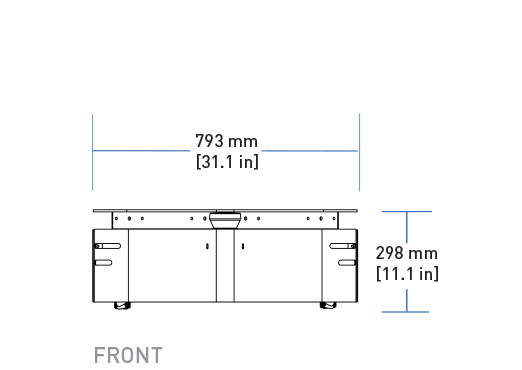
\includegraphics[width=\textwidth]{rb_front}
%        \caption{Front}
%        %\label{fig:gull}
%    \end{subfigure}
%    ~
%    \begin{subfigure}[t]{0.34\textwidth}
%        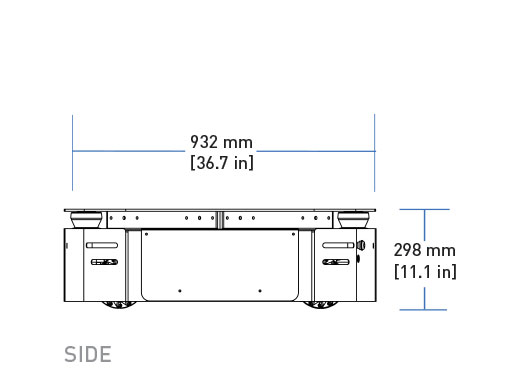
\includegraphics[width=\textwidth]{rb_side}
%        \caption{Side}
%        %\label{fig:gull}
%    \end{subfigure}
%     %add desired spacing between images, e. g. ~, \quad, \qquad, \hfill etc. 
%      %(or a blank line to force the subfigure onto a new line)
%    \begin{subfigure}[t]{0.34\textwidth}
%        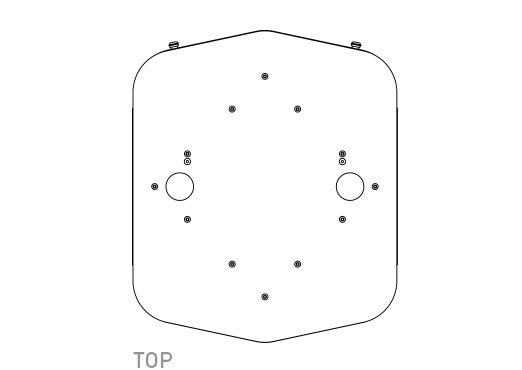
\includegraphics[width=\textwidth]{rb_top}
%        \caption{Top}
%        %\label{fig:tiger}
%    \end{subfigure}
%     ~%add desired spacing between images, e. g. ~, \quad, \qquad, \hfill etc. 
%    %(or a blank line to force the subfigure onto a new line)
%    \begin{subfigure}[t]{0.34\textwidth}
%        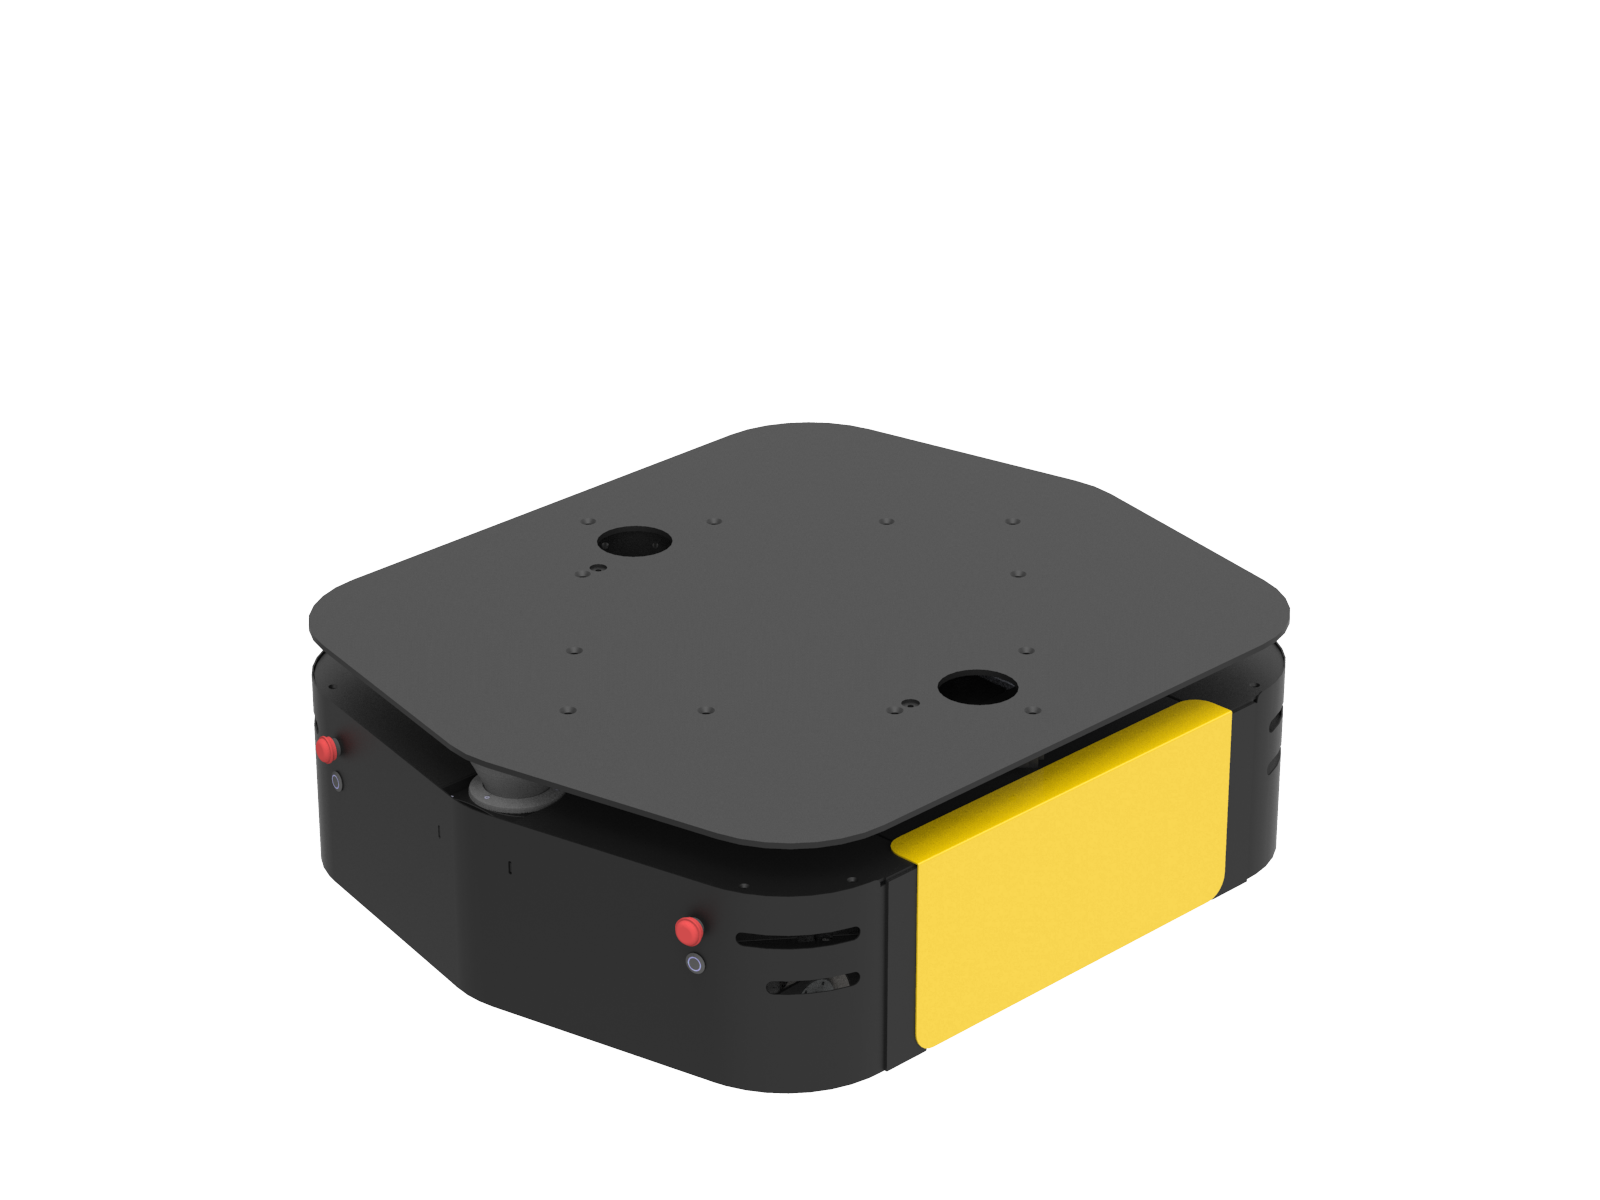
\includegraphics[width=\textwidth]{ridgeback}
%        \caption{Render}
%        %\label{fig:mouse}
%    \end{subfigure}
%    \caption{The Ridgeback mobile platform}\label{fig:ridgeback}
%\end{figure*}
\begin{figure}[h]
\begin{floatrow}
    \ffigbox{
        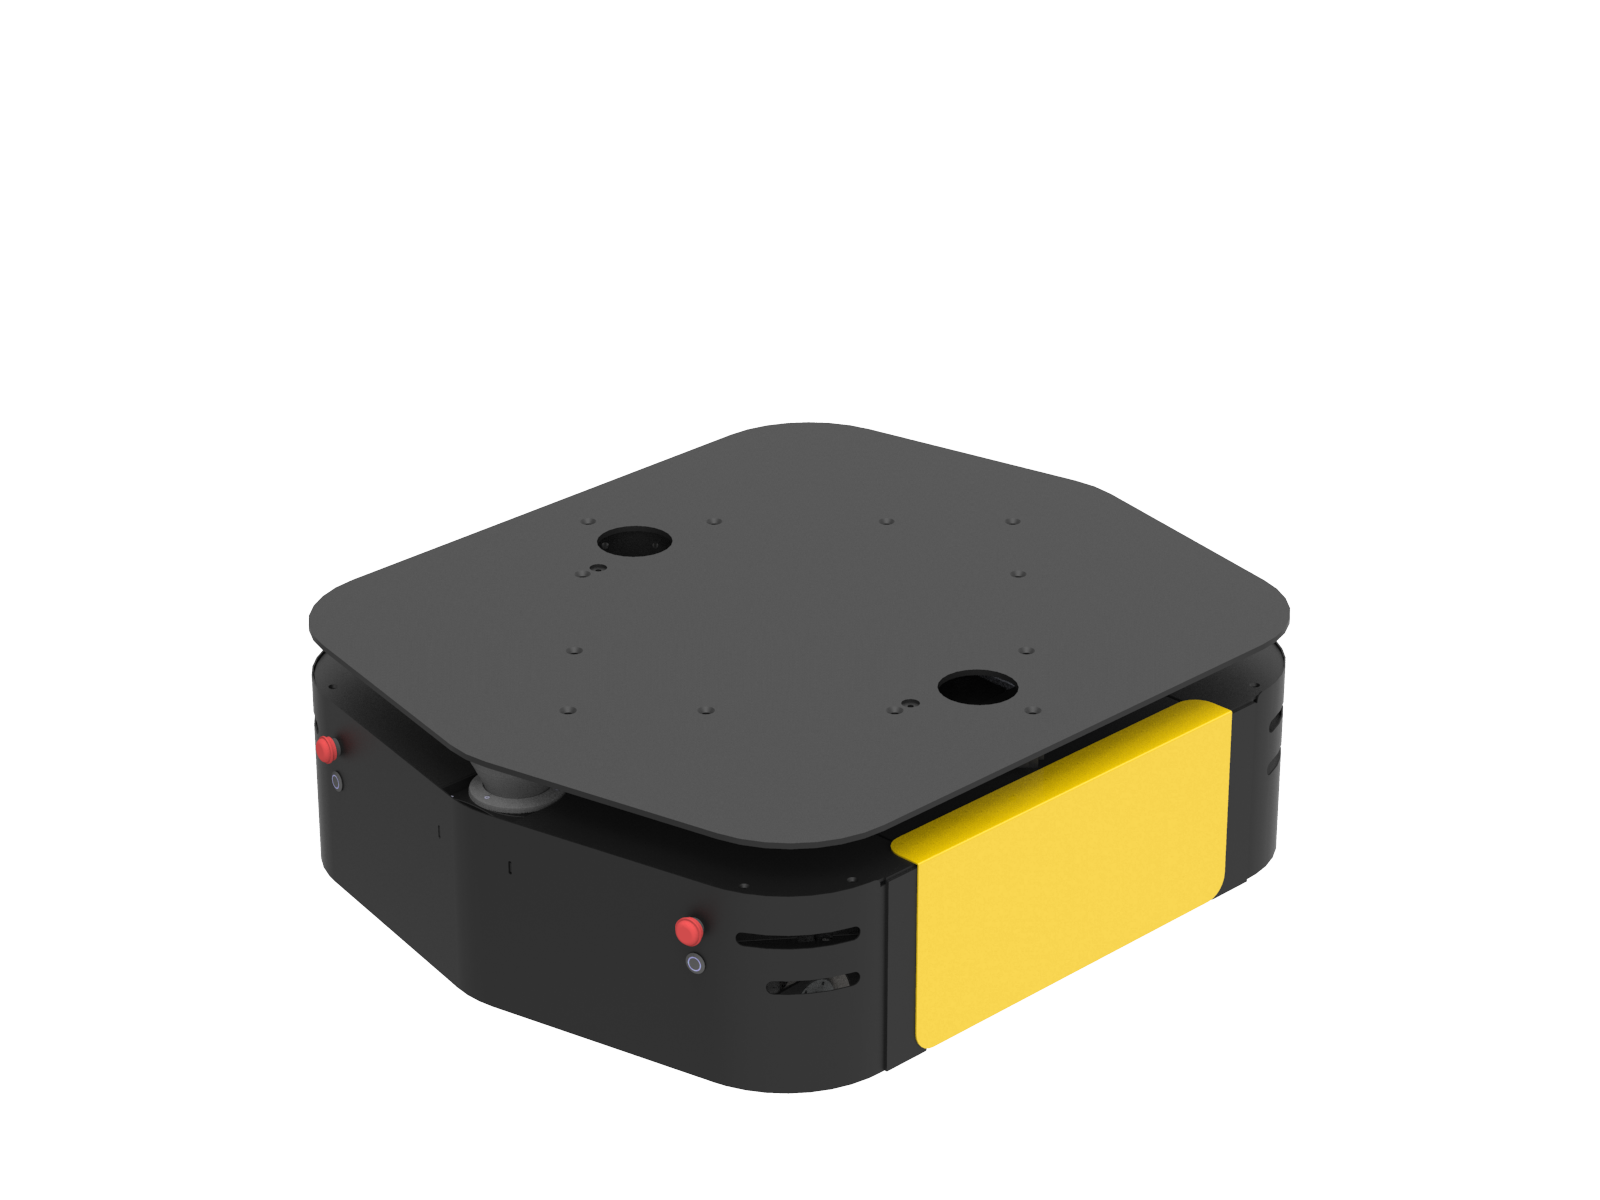
\includegraphics[width=0.49\textwidth]{ridgeback}
        }{
    \caption{The Ridgeback mobile base}\label{fig:ridgeback}
    }
    \capbtabbox{
\begin{tabular}{@{}lll@{}}
\toprule
\textbf{{ Weight}}&  135 kg& \\ \midrule
\textbf{{Payload}}&  100 kg&  \\ \midrule
\textbf{{Dimensions}}&  {\footnotesize Width: 793 mm}&  \\
&  {\footnotesize Length: 960 mm}&   \\
&  {\footnotesize Height: 296 mm}& \\ \midrule
\textbf{{Max Speed}}& 1.1 m/s& \\ \midrule
\textbf{Power}& average 800 W& \\ \bottomrule
\end{tabular}
}{
\caption{Ridgeback specifications}
\label{tab:ridgeback_specs}
}
\end{floatrow}
\end{figure}
It is primarily designed for warehousing applications as it is highly flexible in a controlled flat environment.
The built in wheel odometry provides accurate local position estimates, with pose drift accumulating very slowly.
For improved localization and obstacle avoidance, the navigation stack ROS package provides SLAM capability using the on-board LIDAR and IMU.

In a controlled laboratory setting, this platform enables a high degree of flexibility in research.
The high load bearing capability enables the platform to carry manipulators (such as the UR10) and large sensor arrays.
Other modifications to the structure are also possible as there is a large amount of space available on the platform. 

\newpage
\section{UR10} 
The UR10 is Universal Robotics largest collaborative industrial manipulator.
It is a full 6DOF robotic arm capable of mimicking human arm movements.
During operation it can handle weights up to 10 kg, making it viable for a wide range of tasks.
The provided drivers enable performing collaborative tasks alongside human operators, allowing for easy positioning of the arm through compliant movement and preventing use of excessive force on impact.
\begin{figure}[h]
\begin{floatrow}
    \ffigbox{
        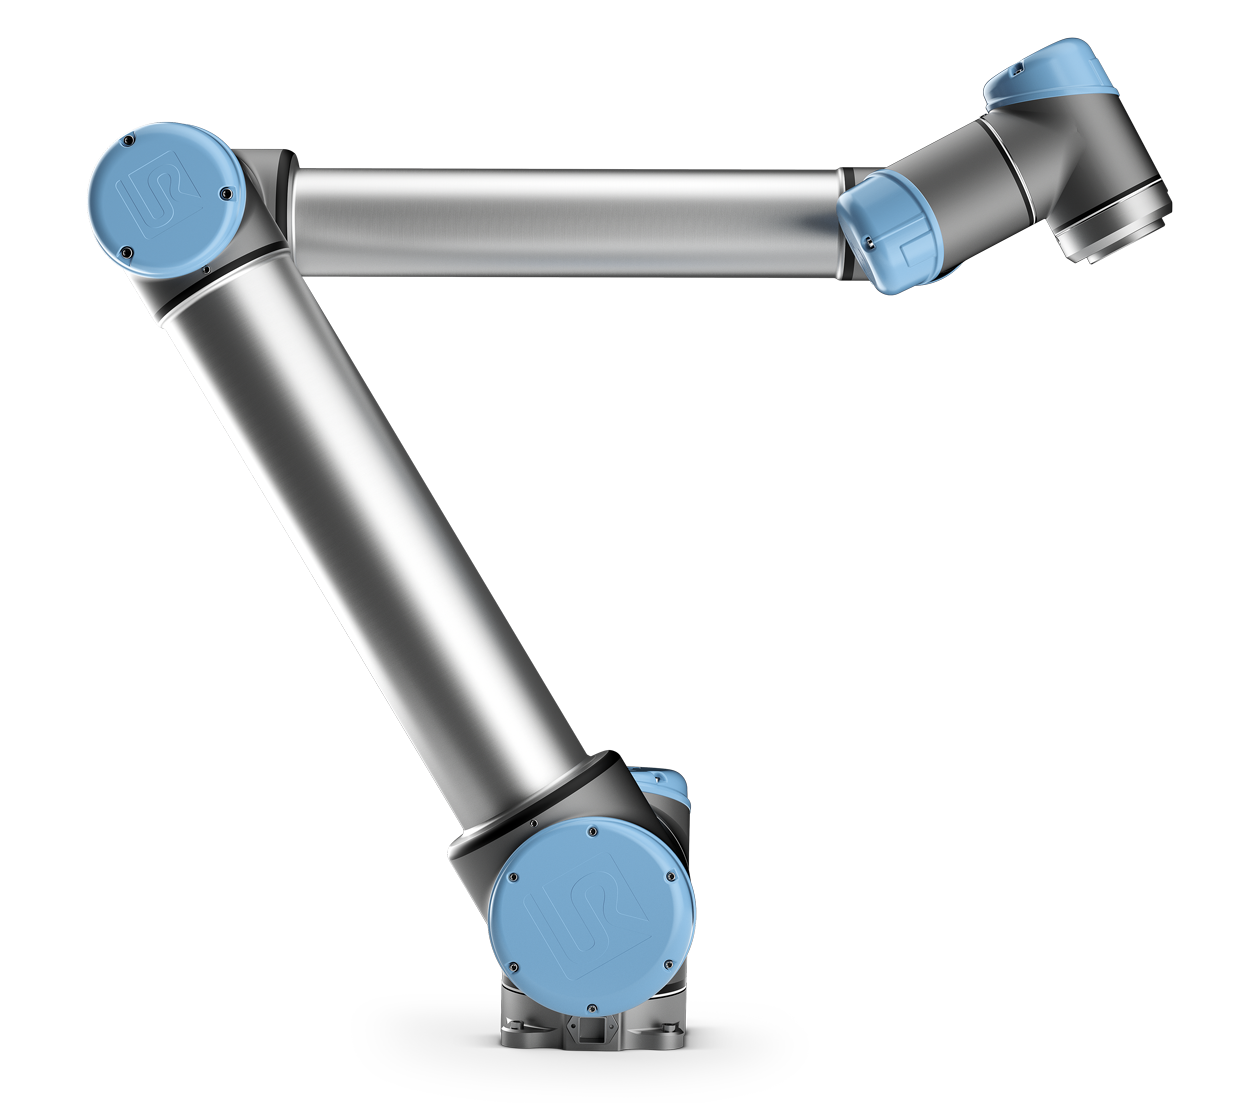
\includegraphics[width=0.34\textwidth]{ur10_right}
        }{
    \caption{The UR10 manipulator}\label{fig:ur10}
    }
    \capbtabbox{
\begin{tabular}{@{}lll@{}}
\toprule
\textbf{{ Weight}}&  28.9 kg& \\ \midrule
\textbf{{Payload}}&  10 kg&  \\ \midrule
\textbf{{Speed}}&  {\footnotesize Large joints: Max 120$^{\circ}$/s}&  \\
&  {\footnotesize Wrist joints: Max 180$^{\circ}$/s}&   \\
&  {\footnotesize Tool: approx 1 m/s}& \\ \midrule
\textbf{{\small Repeatability}}& $\pm0.01$ mm& \\ \midrule
\textbf{Power}& average 350 W& \\ \bottomrule
\end{tabular}
}{
\caption{UR10 specifications}
\label{tab:ur10 specs}
}
\end{floatrow}
\end{figure}

The data in table \Cref{tab:ur10 specs} clearly shows that the UR10 manipulator is meant for tasks involving high precision and light payloads. 
The repeatability value of $0.01$ mm shows that the UR10 can reach the same pose multiple times with a high degree of accuracy, which is important in industrial applications.
Additionally, it's light weight and high end-effector modularity make it ideal for research purposes.

\chapter{State estimation}\label{chapter:State estimation}
State estimation is an often encountered challenge when working with autonomous systems.
Most autonomy schemes require accurate information on the current state of the system in order properly modify the system behaviour.
This type of system can be generalized as a non-linear system described by a difference equation and observation model with additive noise \footnote{we leave out separate expressions for input variables as they can be integrated within the functions $f$ and $h$}
\begin{subequations}\label{eq:state_space_nl}
\begin{gather}
x_k = f\left(x_{k-1}\right) + w_{k-1} , \ x \in \mathbb{R}^n \\
z_k = h\left(x_k\right) + v_k, \ z \in \mathbb{R}^k
\end{gather}
\end{subequations}
Finding the state estimate $\hat{x}_k$ given the measurements $z_0 \dots z_k$ subject to measurement noise $v$ and past states $x_0 \dots x_{k-1}$ subject to process noise $w$ is the state estimation problem.
Various algorithms have been developed using different mathematical frameworks to find the best estimate according to some optimality criterion (\cite{thrun2005probabilistic}).  
\begin{figure}[h]
\centering
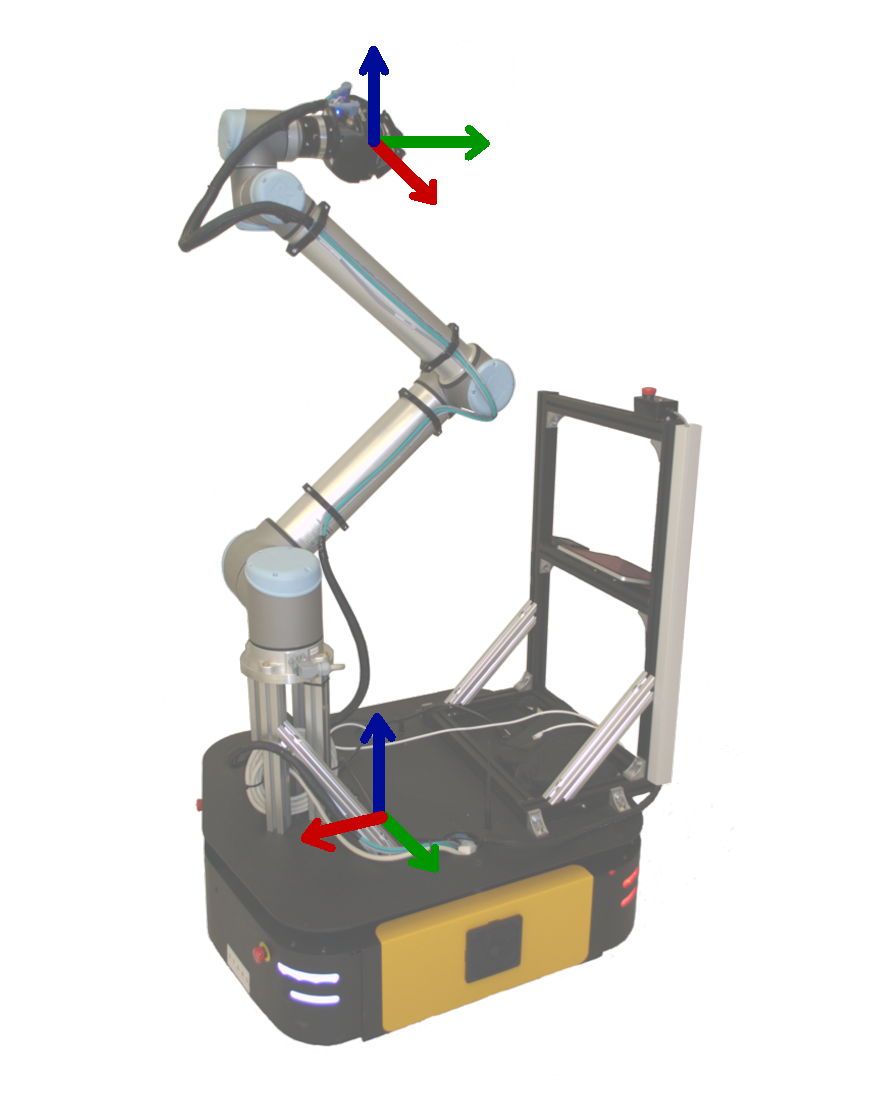
\includegraphics[scale=0.4]{Thingtr}
\caption{The Thing mobile manipulator and the frames subject to estimation}
\label{figure:thing states}
\end{figure}

The problem of state estimation for a mobile manipulator is twofold: it is necessary to estimate the state of the end-effector in the local workspace while also placing it in the global context of a map or starting position.
The local state of the end-effector is successfully estimated using a deterministic kinematic model.
Joint position values are used to provide a state estimate, ignoring various dynamic and environment effects.
Estimating the base state (\textit{localization}) is a more complex problem; the dynamic and environment effects on base movement significantly affect the steady-state.
Consequently, in addition to kinematic models we have to rely on movement estimates from sensor data which is inherently noisy.
The imperfect model and sensor data are fused in a single estimate using a probabilistic framework.

In this chapter, we first define our state of interest (as seen in \Cref{figure:thing states}) in \Cref{section:State}. 
Section \Cref{section:Kinematics} contains details on the derivation of the kinematic model used in end-effector state estimation assuming sufficient knowledge of the base pose. 
The probabilistic framework used for estimating the base state is described in \Cref{section:Localization}, where wheel and LIDAR odometry are fused to provide an accurate estimate.
%The focus of this chapter is estimating the pose of the end-effector and mobile base, but the methods are extendable to any frame on the platform.

\section{State}\label{section:State}
Control and task algorithms frequently require information on the pose of the mobile manipulator frames in Cartesian space. 
A frame pose represents complete information about a frames position and orientation in a given reference frame.
The pose is often represented by a \textit{homogenous transformation matrix}
\begin{align}
T_{k-1}^k =
\begin{bmatrix}
R & p\\
0 & 1\\
\end{bmatrix}\,.
\label{eq:transform}
\end{align}
The rotation matrix $R \in \mathbb{R}^{3x3}$ represents the orientation of the frame $k$ relative to the frame $k-1 $, while translation is represented by the vector $p \in \mathbb{R}^3$.
Estimating the matrix $T$ for the end-effector is a 9-dimensional problem which can be further reduced. 
It is possible to fully define it the vector $r$ consisting of the translation vector $p$ and a \textit{quaternion} $q$
\begin{align} 
r_{EE}\left(T_{0}^{EE}\right) = 
\begin{bmatrix}
x& y& z& q_w& q_x& q_y& q_z
\end{bmatrix}^T\, .
\label{eq:pose}
\end{align}
The number of dimensions can also be reduced for the base, as it moves on a 2D plane and thus only rotates alongside one axis and has a constant $z$ coordinate
\begin{align}\label{eq:pose base}
r_{B}\left(T_{0}^{B}\right) = 
\begin{bmatrix}
\hat{x}& \hat{y}& \hat{\theta}
\end{bmatrix}^T\, .
\end{align}
The estimated state consists of end-effector and base poses comes in the form of a 10-dimensional \textit{task vector} $s$
\begin{align}\label{eq:task_vector}
s = 
\begin{bmatrix}
r_{EE}& r_B
\end{bmatrix}^T
\end{align}
Using this representation, the state estimation problem has been reduced from 24 down to 10 dimensions.
Reducing the dimensionality of the problem makes it computationally less expensive, which is vital for real-time operation.
Considering that the global state estimate in this work is derived exclusively from base odometry data, it is possible to infer the base pose knowing the end-effector pose.
However, to maintain generality the formulation in \eqref{eq:pose} and \eqref{eq:pose base} is kept.

\section{Kinematic model}\label{section:Kinematics}
Disregarding the various dynamic and environment effects, the Thing can be modelled as manipulator.
The Ridgeback platform is system with holonomic constraints and it's global position and the orientation can be viewed as a chain of two prismatic and a rotational joint. 
These three joints make up the base upon which we add the kinematic model of the UR10 manipulator.
This results in a system kinematically indistinguishable from a redundant manipulator.

The UR10 joint position measurements are reasonably accurate and thus this model can be used to produce a valid local end-effector state estimate.
Assuming valid estimates for the base position and orientation, this model will accurately represent the global state of the mobile manipulator.
\subsection{Forward kinematics}\label{subsection:FK}
Forward kinematics are defined as a set of equations that express the pose of a certain frame on a kinematic chain as a function of configuration-space values
\begin{align}\label{eq:config_matrix}
q = 
\begin{bmatrix}
q_0& q_1& q_2& q_3& q_4& q_5& \hat{x}& \hat{y}& \hat{\theta}
\end{bmatrix}^T \quad .
\end{align}
The first six elements $q_i$ represent UR10 joint angles, while the last three values represent the base pose estimate.
The equations are commonly derived using the transforms defined in \eqref{eq:transform}.
The transform between two frames can be defined as a function of only four parameters using the Denavit-Hartenberg notation \citep{uicker1964iterative}.
\begin{align}
T_{k-1}^k(d, \ \theta, \ a, \ \alpha)
=
\begin{bmatrix}
\cos\theta_{k}& -\cos\alpha_{k}\sin\theta_{k} & \sin\alpha_{k}\sin\theta_{k} & a_k\cos\theta_{k}\\
\sin\theta_{k}& \cos\alpha_{k}\cos\theta_{k} & -\sin\alpha_{k}\cos\theta_{k} & a_k\sin\theta_{k}\\
0 & \sin\alpha_{k} & \cos\alpha_{k} & d_{k}\\
0 & 0 & 0 & 1\\
\end{bmatrix} \quad .
\label{eq:homogenous}
\end{align}
The parameters $a, \alpha$ are usually constant and represent the structure, while $d, \theta$ represent the prismatic and rotational joint values and biases.
Using the DH parameters as defined in \Cref{DH}, we derive all the transforms \eqref{eq:homogenous} from global frame to the end effector frame.
Multiplying these transforms gives us the transform from the global frame to any frame of the mobile manipulator
\begin{equation}
T_{0}^{EE} = \prod_{k=1}^{N_{EE}} T_{k-1}^{k} \quad .
\label{FK}
\end{equation}
The forward kinematics model is subject to various joint angle and link length biases, as it is possible the given DH parameters do not exactly correspond to the physical manipulator.
However, the estimate provided has a significantly lower error than that of base localization and thus can be disregarded in the current analysis.

It is also interesting to note that the forward kinematics equations are non-injective surjective functions: 
every $q$ corresponds to a single pose $T$, even though a given $T$ might correspond to multiple or infinite values of $q$.
The analytic formulation of the transform from the global frame to the end-effector can be found in the appendix.

\subsection{Differential forward kinematics}
Equations defined in \Cref{subsection:FK} provide an estimate of the mobile manipulator state \eqref{eq:task_vector} using the configuration vector $q$. 
However, algorithms used in motion planning and trajectory optimization require an estimate on how configuration change affects the state.
This information is contained within the manipulator Jacobian $J$.
We define the Jacobian $J$ as the derivative of the function $f\left(x\right) \ : \mathbb{R}^n \rightarrow \mathbb{R}^k $ with respect to the vector $x$.
\begin{align}\label{eq:jacobian}
J =
\begin{bmatrix}
    \dfrac{\partial {f_1}}{\partial x_{1}}      & \dfrac{\partial {f}_{1}}{\partial x_{2}}  & \dots & \dfrac{\partial {f}_{1}}{\partial x_{n}}  \\
    \dfrac{\partial{f_2}}{\partial x_{1}}      & \dfrac{\partial {f}_{2}}{\partial x_{2}}  & \dots & \dfrac{\partial {f}_{2}}{\partial x_{n}} \\
    \vdots \\
    \dfrac{\partial {f_k}}{\partial x_{1}}      & \dfrac{\partial {f}_{k}}{\partial x_{2}}  & \dots & \dfrac{\partial {f}_{k}}{\partial x_{n}}
\end{bmatrix}\, .
\end{align}
Now $\dot{f}$ can be calculated by multiplying the matrix with $\dot{x}$
\begin{align} \label{eq:jacobian_identity}
\dot{f} = J \dot{x}\, .
\end{align}
For a sufficiently small $\Delta$, \eqref{eq:jacobian_identity} can be extended to produce a first order approximation $\hat{f}_k$ 
\begin{align} \label{eq:jacobian_estimate}
\hat{f}_k = f_{k-1} + J\left(x_{k} - x_{k-1}\right)\, .
\end{align}
This framework can be employed in various state estimation and motion planning algorithms.
\newpage
\subsubsection{End-effector Jacobian}
For motion planning applications, an estimate on how configuration change affects the end-effector pose $\Delta r_{EE}$ is vital.
The end-effector Jacobian is defined as the derivative of the end-effector pose \eqref{eq:pose} with respect to the configuration vector $q$.
While it can be derived analytically, it is often advantageous to derive it using the geometry of the chain.
Here the Jacobian takes the form 
\begin{equation}
J =
\begin{bmatrix}
J_{v} \\ 
J_{\omega}
\end{bmatrix}\, ,
\label{jacob1}
\end{equation}
where the matrix $J_v$ is the position Jacobian and $J_{\omega}$ matrix is the orientation Jacobian.
In this case, the components representing orientation change are equal to the rotation axes of the joint $q_j$
\begin{align}
J_{\omega_j} = \dfrac{\partial o}{\partial q_j} = z_{j}\, .
\end{align}
The components representing position difference for rotational joints are
\begin{equation}
J_{v_j} = \dfrac{\partial p}{ \partial q_{j}} = z_j \times (w - p_j)\, .
\end{equation}
For prismatic joints the orientation component is $J_{\omega_j} = 0$, while the translational component lies on the $z$ axis
\begin{equation}
J_{v_j} = \dfrac{\partial p}{ \partial q_j} = z_j\, .
\end{equation}
As seen in \Cref{algorithm:jacobian calc}, the geometric derivation is suitable for software implementation as it does not require symbolic calculations and relies only on matrix operations.
\begin{algorithm}[h]
 \KwData{Kinematic chain transforms $T_{i}$ and joint type flags $rev_i$} 
 \KwResult{End-effector Jacobian matrix $J$}
 $T=I$\;
 \For{$i = 1, 2, ..., N$}{
 $T = TT_{i}$\tcc*[r]{get next transform}
 $R_i = R(T)$\;
 $O_{i} = O(T)$\;
 \eIf(\tcc*[h]{element corresponding to the base joint}){$i = 1$}{
 	$z_i = (rev_i)\mathbf{1}$\;
 	$v_i = (rev_i)z_i \times w + (1-rev_i)z_i$\;
 }(\tcc*[h]{all subsequent joints}){
  	$z_i = (rev_i)R_{i-1}\begin{bmatrix}0& 0& 1\end{bmatrix}^T$\;
 	$v_i = (rev_i)z_i \times (r - O_{i-1}) + (1-rev_i)z_i$\;
 }
 }
 $J = \begin{bmatrix}v &z \end{bmatrix}^T$ \tcc*[r]{compose the Jacobian}
 \caption{Geometric Jacobian calculation}
 \label{algorithm:jacobian calc}
\end{algorithm}
The \textit{twist} vector $w$ is defined as the composition of translational and rotational velocities.
For a sufficiently small pose difference $\Delta r$, the vectors are approximately equal
\begin{align}\label{eq:pose_diff}
w  = 
\begin{bmatrix} 
v \\ \omega 
\end{bmatrix} 
\approx 
\begin{bmatrix}
\Delta p \\
\Delta o
\end{bmatrix}
= 
\Delta r \, .
\end{align}
Calculating the position difference is straightforward and comes down to subtracting the goal and current positions
\begin{align}
\Delta p = p - p_{goal}\, .
\end{align}
The orientation difference is calculated as follows \citep{sciavicco2012modelling}
\begin{subequations}\label{eq:pose difference}
\begin{gather}
\Delta o = 0.5 L^{-1} \left( n_c\times n_d + s_c\times s_d + a_c\times a_d \right)\, , \\
L = - 0.5 \left(\left[n_c\right]_{\times}\left[n_d\right]_{\times} + \left[s_c\right]_{\times}\left[s_d\right]_{\times} 
+ \left[a_c\right]_{\times}\left[a_d\right]_{\times} \right)\, .
\end{gather}
\end{subequations}
Plainly stated, this is the equivalent of angular velocity defined by two different orientations.
\section{Localization}\label{section:Localization}
When using the kinematic model in \Cref{section:Kinematics} sufficiently accurate base pose estimates $\hat{x},\hat{y},\hat{\theta}$ are assumed.
In reality, obtaining accurate pose estimates is non-trivial and often requires fusing sensor data while taking in to account the probabilistic nature of measurements.

Localization of the Thing mobile manipulator employs a motion model of the omni-directional drive on the Ridgeback and data provided by the LIDAR.
The wheel and LIDAR odometry provide Cartesian velocity estimates with covariance data.
This data is fused using an extended Kalman filter and the resulting estimate is more accurate (in theory) than simply integrating wheel odometry data.
\subsection{Wheel odometry}
In classical mechanics a system may be defined as \textit{holonomic} if all constraints of the system are holonomic. For a constraint to be holonomic it must be expressible as a function:
\begin{align}
f(x_1,\ x_2,\ x_3,\ \ldots,\ x_N,\ t)=0
\end{align} 
i.e. a holonomic constraint depends only on the coordinates $x_j$ and time $t$. It does not depend on the velocities or any higher order derivative with respect to time $t$.
Decoupled translational and angular velocities make the estimation process less prone to error, as angular velocities are usually much more difficult to estimate.
Having wheel encoder velocity readings $w_0,w_1,w_2,w_3$, a base twist estimate $\hat{\xi}$ can be calculated
\begin{align}
%\begin{bmatrix}
%\dot{\hat{x}} \\
%\dot{\hat{y}} \\
%\dot{\hat{\theta}}
%\end{bmatrix}
\hat{\xi}
= 
\frac{R}{4}
\begin{bmatrix}
1 &1 &1 &1 \\
-1 &1 &-1 &1 \\
-\frac{1}{k} &-\frac{1}{k} &\frac{1}{k} &\frac{1}{k}
\end{bmatrix}
\begin{bmatrix}
w_0 \\
w_1 \\
w_2 \\ 
w_3
\end{bmatrix} \quad .
\label{eq:base vel estimate}
\end{align}
Integrating the velocities from \eqref{eq:base vel estimate} makes it possible to localize the base relative to the starting position.
Odometry estimates are assumed to have a normal distribution, accounting for measurement noise and kinematic nature of the model that ignores dynamic effects.
\begin{equation}\label{eq:wheel_sigma}
\xi \sim \mathcal{N}(\mu_\xi,\,\Sigma)\,.
\end{equation}
The covariance matrix $\Sigma$ in \eqref{eq:wheel_sigma} is set to a constant value empirically found to sufficiently represent estimate uncertainty
\begin{align}
\Sigma 
=
diag\left(0.001,0.001,0.001,100000,100000,0.03\right)\,.
%\begin{bmatrix}
%0.001& 0& 0& 0& 0& 0 \\
%0& 0.001& 0& 0& 0& 0 \\
%0& 0& 0.001& 0& 0& 0 \\ 
%0& 0& 0& 1000000& 0& 0 \\
%0& 0& 0& 0& 1000000& 0 \\
%0& 0& 0& 0& 0& 0.03 
%\end{bmatrix}
\end{align}
\subsection{LIDAR odometry}\label{subsection:lidar_odometry}
A velocity estimate can also be obtained using 
The Hokuyo LIDAR presents itself as a rich source of information on the environment which can be used to estimate base velocity.
Various algorithms exist that implement LIDAR odometry, they are mostly based on Iterative Closest Point matching (ICP) \citep{besl1992method}.
In this work we use the a range flow-based approach available in the form of the \verb|rf2o_laser_odometry| ROS package.

While this work does not cover the details of this algorithm, the formulation is relatively straightforward.
Given a base twist $\mathbf{\xi}$, for every point sensed by the LIDAR a geometric residual $\rho\left(\mathbf{\xi}\right)$ is defined 
\begin{equation}
\begin{split}
\rho\left(\mathbf{\xi}\right) &= R_t + \left(x\sin\theta - y\cos\theta - R_\alpha k_\alpha\right)\omega + \left(\cos\theta + \frac{R_\alpha k_\alpha \sin\alpha}{r}\right)v_x \\
 &+ \left(\sin\theta + \frac{R_\alpha k_\alpha \cos\alpha}{r}\right)v_y\, .
 \end{split}
\end{equation}
To obtain an accurate estimate, the sensor motion is computed by minimizing all geometric residuals within the cost function $F$:
\begin{align}
F\left(\rho\right) &= \frac{k^2}{2}\ln{\left(1 + \left(\frac{\rho}{k}\right)^2\right)}\, , \\
\hat{\xi} &= \min\limits_{\xi} \sum\limits_{i=1}^{N} F \left(\rho_i \left( \mathbf{\xi} \right) \right)\, .
\end{align}
Details on parameters and minimization procedure can be found in \citep{jaimez2016planar}.

\subsection{Extended Kalman filter}
The wheel and LIDAR odometry data is fused using an Extended Kalman Filter \footnote{EKF in rest of text} \citep{fujii2013extended}.
A process and observation model is used to represent the movement of the Thing mobile manipulator:
\begin{subequations}\label{state_space_nl2}
\begin{gather}
x_k = f\left(x_{k-1}\right) + w_{k-1} , \ x \in \mathbb{R}^n\, , \\
z_k = h\left(x_k\right) + v_k, \ z \in \mathbb{R}^k\, .
\end{gather}
\end{subequations}
Without going in to detail on the derivation of the EKF algorithm, it can be described as having two steps.\:
the model forecast step uses the motion model and last estimated state $\hat{x}_k^+$ to produce an \textit{a priori} estimate of the next state $\hat{x}_k^-$ and covariance $P_k^-$
\begin{subequations}\label{eq:nl_forcast}
\begin{gather}
\hat{x}_k^- = f\left(\hat{x}_{k-1}^+\right) \\
P_k^- = J_f\left(\hat{x}_{k-1}^+\right)P_{k-1}^+J_f^T\left(\hat{x}_{k-1}^+\right) + Q_{k-1}
\end{gather}
\end{subequations}
The correction step makes use of local sensor odometry to calculate the \textit{Kalman gain} $K_k$ and produce \textit{a posteriori} estimates $\hat{x}_k^+$ and $P_k^+$ 
\begin{subequations}\label{eq:nl_correction}
\begin{gather}
\hat{x}_k^+ \approx \hat{x}_k^- + K_k\left(z_k - h\left(\hat{x}_k^-\right)\right) \\
P_k^+ = \left(I - K_kJ_h\left(\hat{x}_k^-\right)\right)P_k^- \\
K_k = P_k^-J_h^T\left(\hat{x}_k^-\right)\left(J_h\left(\hat{x}_k^-\right)P_k^-J_h^T\left(\hat{x}_k^-\right) + R_k\right)^{-1} 
\end{gather}
\end{subequations}
The $J_f$ and $J_h$ matrices in \eqref{eq:nl_forcast} \eqref{eq:nl_correction} represent the process and measurement model Jacobians, while the process and measurement noise covariance is represented by the $Q$ and $R$ matrices.
Estimates provided by \eqref{eq:nl_forcast} \eqref{eq:nl_correction} are first-order estimates, higher order estimators of this type exist but are computationally infeasible for real-time applications.

It is also important to note that the EKF assumes white Gaussian noise and thus can only be successfully applied when the actual process and measurement noise have a near-Gaussian distribution.


\chapter{Motion planning}\label{chapter:motion planning}
As mentioned in \Cref{chapter:State estimation}, the primary motion planning objective consists of reaching the desired pose with the end-effector and mobile base.
However, moving the mobile manipulator safely and efficiently in the workspace is more involved and significantly constrains the primary objective. 
For instance, it is important to maintain distance from obstacles both with the platform and the manipulator.
Additionally, various other performance metrics exist which may need to be maximized or maintained above a certain value.
These objectives and constraints can be formalized in a way that fits the motion planning problem.

In \Cref{section:inverse kinematics} the \textit{inverse kinematics} problem is considered for mobile manipulator.
This involves finding an configuration $q$ that corresponds to a given end-effector pose $r$.
Section \ref{section:redundancy resolution} explores the problem of utilizing the extra degrees of freedom of the system to optimize movement, also referred to as \textit{redundancy resolution}.
The remaining sections explore two different approaches to redundancy resolution: \textit{task-priority} and s\textit{equential convex optimization}. 
The classic task-priority algorithm is computationally efficient extension to the optimization approach for inverse kinematics, but also highlights the drawbacks of a purely linear optimization algorithm.
A more contemporary approach of sequential convex optimization provides a more general and powerful optimization infrastructure that is highly modular, at the cost of computational efficiency.
\section{Inverse kinematics}\label{section:inverse kinematics}
Regulating kinematic tasks that are configuration dependent reduces to the problem
\begin{align}
f\left(q\right) = 0 \, . %% TODO check this
\end{align}
where $q \in \mathbb{R}^{n} $  is the configuration vector. 
The classical approach to inverse kinematics would have us find the inverse of the function $f$
\begin{align}
q = f^{-1}\left(0\right)\, . \label{eq:inverse}
\end{align}
However, this inverse can only exist in non-redundant configurations, otherwise the number of solutions is infinite.
Even in cases where the configuration is non-redundant , the inverse function is still occasionally impossible to derive.
In order to solve this problem, an optimization approach which avoids dealing with complicated analytical expressions is employed.
\subsection{Differential inverse kinematics}
In an inverse differential kinematics scheme used for redundant kinematic chains, $f\left(q\right)$ is regulated to the target value using
\begin{align}
\label{diffik_1}
\frac{\partial}{\partial q}f = -\lambda_{f}f\left(q\right), \lambda_{f} > 0 \, .
\end{align}
The solution to \eqref{diffik_1} is often rank-deficient, so a least squares formulation is employed
\begin{align}
\label{diffik_2}
\min\limits_{\dot{q}} & \frac{1}{2}\left\Vert\frac{\partial f}{\partial q} \dot{q} + \lambda_{f}f\left(q\right)\right\Vert^2, \lambda_{f} > 0 \, .
\end{align}
Letting $J = \frac{\partial f}{\partial q}$ and $a = -\lambda_{f}f\left(q\right)$, the solution to \eqref{diffik_2} that minimizes the $L_{2}$ norm is given by finding the pseudoinverse of the $A$ matrix
\begin{align}
\label{diffik_4}
\dot{q} = J^{\dagger}a  \, .
\end{align}
\subsection{The Jacobian pseudoinverse and numerical filtering}
In \eqref{diffik_1}-\eqref{rresolution_2}, the pseudoinverse operation denoted by $\dagger$ is defined as 
\begin{align}
J^{\dagger} = J^T\left(JJ^T\right)^{-1}\, .
\end{align}
While more numerically stable than the classic inverse operator in \eqref{eq:inverse}, this method is also subject to \textit{kinematic singularities} in the manipulator.
These are configurations where the linear system requires a large configuration change in order to accomplish a given task space change.
The components of the task Jacobian $\frac{\partial f}{\partial q}$ then approach 0, resulting in loss of rank.
Implementing the pseudo-inverse in a numerically stable way is very important for robustness and non-trivial.
\subsubsection{Damped psudoinverse}
We often use the more numerically stable \textit{damped pseudoinverse} \citep{chan1988general}
\begin{align}
J^{\#} = J^T\left(JJ^T + \lambda I\right)^{-1} ,  \lambda \in \mathbb{R}\, .
\end{align}
There are also various contemporary approaches to implementing the pseudoinverse \citep{chiaverini1994review}. 
In this work we use the \textit{selectively damped pseudoinverse} \citep{buss2005selectively}, alongside with \textit{singular value filtering} described in \citep{colome2015closed}.
\subsubsection{Selectively damped pseudoinverse}
The matrix pseudoinverse operation can be performed using an SVD decomposition of the Jacobian
\begin{align}
& \ \ \ \ \ J = \sum\limits_{i}{\sigma_{i}u_iv_i^T}\, , \\
J^T&\left(JJ^T\right)^{-1} = \sum\limits_{i}{\frac{1}{\sigma_{i}}v_iu_i^T}\, .
\end{align}
The pseudoinverse would in this case have the form 
\begin{align}
J^T\left(JJ^T + \lambda I\right)^{-1} = \sum\limits_{i}{\frac{\sigma_{i}}{\sigma_{i}^2 + \lambda}v_iu_i^T}\, ,
\end{align}
this \textit{selectively damped pseudoinverse} \citep{buss2005selectively} equates to choosing a specific value $\lambda_i$ for each singular value $\sigma_i$
\begin{align}\label{eq:sdp}
J^{\#} = \sum\limits_{i}{\frac{\sigma_{i}}{\sigma_{i}^2 + \lambda_i}v_iu_i^T}\, .
\end{align}
\subsubsection{Singular value filtering}
The singular values of a Jacobian determine it's stability with respect to inversion.
Lower singular values indicate that the matrix is closer to being singular.
A proposed approach to solving this problem prior to using a specific inversion technique is \textit{singular value filtering} \citep{colome2012redundant}. 
This technique sets the lowest singular value of a given jacobian matrix $J$ to $\sigma_0$
\begin{align}\label{eq:svf}
h_{v,\sigma_0}\left(\sigma\right) = \frac{\sigma^3 + v\sigma^2 + 2\sigma + 2\sigma_0}{\sigma^2 + v\sigma + 2}\,.
\end{align}
In \eqref{eq:svf} the shape factor $v$ determines the difference between modified and original singular values $h_{v,\sigma_0}(\sigma)-\sigma$, a higher $v$ results in lower differences. 
This results in a new Jacobian matrix
\begin{align} \label{eq:svf jacobian}
\hat{J}= \sum\limits_{i}{h_{v,\sigma_0}(\sigma_i)u_iv_i^T}\, .
\end{align}
Authors report that combining this filtering method with any of the above pseudoinverse approaches results in higher stability.
\section{Redundancy resolution}\label{section:redundancy resolution}
Given that the valid set of solutions to \eqref{diffik_2} is in an affine subspace $\mathcal{F} \in \mathbb{R}^n$, the minimization scheme for solving a lower priority set of tasks would be
\begin{align}
\label{diffik_3}
\min\limits_{\dot{q} \in \mathcal{F}} & \frac{1}{2}\left\Vert\frac{\partial g}{\partial q} \dot{q} + \lambda_{g}f\left(q\right)\right\Vert^2 , \lambda_{g} > 0\, .
\end{align}
The process of defining additional constraints for a redundant system, thus reducing the affine subspace $\mathcal{F}$ is called \textit{redundancy resolution}.
The general solution to \eqref{diffik_3}, which minimizes the $L_2$ norm of the primary task while making redundant DOFs available to other inputs $z$ has the form
\begin{align}
\label{rresolution_0}
\dot{q} = J^{\#}a + \left(I - J^{\#}J\right)z ,  z \in \mathbb{R}^n\, .
\end{align}
The operator $\left(I - J^{\#}J\right)$ is an orthogonal projector, thus the effect of the control $z$ will not affect the outcome in a way that cancels out the first term. 
\section{Task-prioity kinematics}\label{section:task priority}
In \citep{nakamura1987task,nakamura1990advanced}, \textit{null-space optimization} is utilized to achieve execution of a secondary task $B$ given a primary task $A$
\begin{subequations}
\begin{gather}
\label{rresolution_1}
\dot{q}  = A^{\dagger}a + \left(I - A^{\dagger}A\right)\tilde{B}^{\dagger}\left(b - BA^{\dagger}a\right) + 
\left(I - A^{\dagger}A\right) \left(I - \tilde{B}^{\dagger}\tilde{B}\right)z\, ,\\
\tilde{B}  = B\left(I - A^{\dagger}A\right)\, .
\end{gather}
\end{subequations}
This \textbf{task-priority} approach to inverse kinematics can be extended to any number of tasks \citep{slotine1991general}.
The main weakness of task-priority lies in the fact that lower-priority tasks will often become infeasible, causing the occurrence of an \textit{algorithmic singularity} \citep{baillieul1985kinematic}.
In \citep{chiaverini1997singularity}, a modified approach is introduced , which guarantees robustness 
\begin{align}
\label{rresolution_2}
\dot{q} = A^{\dagger}a + \left(I - A^{\dagger}A\right)B^{\dagger}b + 
\left(I - \left(A \atop B\right)^{\dagger}\left(A \atop B\right)\right)z\, .
\end{align}
Here the trade-off is lower accuracy and slower convergence because the expression is only an approximation of \eqref{rresolution_1}.
\subsection{Motion planning scheme}
The motion planning scheme implemented using the task priority formulation is focused on simplicity and robustness rather than optimal movement.
The primary task is reaching a goal pose with the end effector, which is vital for most mobile manipulator applications. 
The secondary task handles mobile base trajectory following.
As mentioned in \Cref{section:task priority}, this framework can be extended to any number of tasks, but the increasing numerical instability results in diminishing returns.
\begin{align}
\label{rresolution_3}
\Delta q \approx J_{EE}^{\dagger}\Delta r_{EE} + \left(I - J_{EE}^{\dagger}J_{EE}\right)J_{B}^{\dagger}\Delta r_{B}\, .
\end{align}

\subsection{Drawbacks}\label{subsec:tp drawbacks}
The main drawback to task-priority kinematics in \eqref{rresolution_1} and \eqref{rresolution_2} is that they cannot natively handle nonlinear inequality constraints \citep{moe2016set} and equality constraints. 
Having the ability to define this type of constraint in motion planning is important for more complex systems such as mobile manipulators.

There are currently no open-source implementations for task-priority schemes , as the parameters and structure of the 
scheme vary greatly depending on the tasks and kinematic chain structure.
A more general definition of the problem as a non-linear constrained optimization problem would allow us to utilize the vast array of open-source solvers, implementations and solution schemes developed for a wider range of problems.

\section{Sequential convex optimization}\label{section:sqp}
Performing tasks with a kinematic chain can also be formulated as a bounded non-linear optimization problem $P$. 
The non-linear objective function $f$ is minimized subject to non-linear inequality and equality constraints $g , h$, while keeping the parameter vector $x$ within bounds. 
\begin{align}
\label{optik_1}
\begin{array}{rl}
\min\limits_{x} & f(x) \\
\mbox{s.t.} & x \in \left[x_{min}, x_{max}\right] \\
  & g(x) \le C_{g} \\
  & h(x) = C_{h}
\end{array}
\end{align}
We can solve this problem iteratively, by repeatedly constructing and minimizing a convex approximation of the problem $\tilde{P}$ until constraints are satisfied. With $\tilde{f}$ being the quadratic approximation of the objective function $f$,
\begin{align}
\label{optik_2}
\tilde{f}\left(x\right) = f\left(x^k\right) + \nabla f\left(x^k\right)\left(x - x^k\right) + \frac{1}{2}\left(x - x^k\right)^T Hf\left(x^k\right)\left(x - x^k\right)\, .
\end{align}
 and $\tilde{g}, \tilde{h}$ being local affine approximations of constraint functions
 \begin{eqnarray}
 \begin{split}
 \label{optik_3}
\tilde{g}\left(x\right) = g\left(x^k\right) + \nabla g\left(x^k\right)\left(x - x^k\right)\, , \\
\tilde{h}\left(x\right) = h\left(x^k\right) + \nabla h\left(x^k\right)\left(x - x^k\right)\, . 
\end{split}
\end{eqnarray}
Using quadratic programming (QP) techniques, we solve $\tilde{P}$
\begin{align}
\label{optik_4}
 \begin{array}{rl}
\min\limits_{x} & \mathcal{L}\left(x,\mu\right)\\
\mbox{s.t.} & x \in \left[x_{min}, x_{max}\right]\, .
\end{array}
\end{align}
Where $\mathcal{L}\left(x,\mu\right)$ represents the problem Lagrangian
\begin{align}
\label{optik_5}
\mathcal{L}(x,\mu) = \tilde{f}\left(x\right) + \mu\sum\limits_{i = 1}^{i_{max}}{\tilde{g}_{i}\left(x\right)}
+ \mu\sum\limits_{j = 1}^{j_{max}}{\tilde{h}_{j}\left(x\right)}\, .
\end{align}
The Lagrange multiplier $\mu > 0 \in \mathbb{R}$ is a large positive value that regulates the priority of constraints over the objective function. Setting a sufficiently large value for $\mu$ turns the problem into a constraint satisfaction problem
\begin{align}
\label{optik_6}
\mathcal{L}(x,\mu) \approx \sum\limits_{i = 1}^{i_{max}}{\tilde{g}_{i}\left(x\right)}
+ \sum\limits_{j = 1}^{j_{max}}{\tilde{h}_{j}\left(x\right)}\, ,
\end{align}
ignoring main objective function minimization in lieu of satisfying constraints.
\subsection{Modeling objective and constraint functions}
The objective function $f\left(x\right)$ can include various terms relating to kinematic and dynamic behaviour of the kinematic chain.
An important thing to keep in mind is that these constraints
\subsubsection{Minimizing state change}
In kinematic planning $f\left(x\right)$ is often employed to keep the chain in a configuration close to the seed configuration $x_{seed}$
\begin{align}
\label{optik_7}
f\left(x\right) = \left(x - x_{seed}\right)W\left(x - x_{seed}\right)^{T}\, .
\end{align}
This results in more predictable solutions to the problem, often avoiding non-modelled dynamic constraints resulting from large changes in configuration.

\subsubsection{Pose control}
We regulate the execution of a pose goal $r$ using equality constraint functions of the type
\begin{align}
\label{eq:optik_8_aux}
\Delta r = 0\, .
\end{align}
Convexifying \eqref{eq:optik_8_aux} results in the familiar linear equation
\begin{align}
\label{eq:optik_8}
h\left(x\right) = \left\vert J\left(x - x_{k}\right) - \Delta r \right\vert = 0\, .
\end{align}
In the case of a Cartesian task-space, the error between target pose and current pose in \eqref{eq:optik_8} can be represented in the form of a 6D vector
\begin{align}
\Delta r = \log\left(T_{target}^{-1}\left(a\right) T_{current}\left(x\right)\right)\, .
\end{align}
The $\log$ operator here is the matrix $\log$ operator.
This vector can also be obtained using identities \eqref{eq:pose difference}.

\subsubsection{Obstacle avoidance}
Obstacle avoidance can be handled as an inequality constraint in the NL optimization problem.
The simplest way of implementing this is using the constraint function
\begin{align}
g\left(x\right) = \left\vert p_{base} - p_{obstacle} \right\vert \leq Rq, .
\end{align}
This can in turn be extended to any number of obstacles.
Collision checking libraries are often used to find a set of closest points for which to optimize.
\subsubsection{Manipulability maximization}
Having a metric $M$ that describes the distance from singularity of the system Jacobian, we could use the scheme in \eqref{optik_1} to optimize task execution.
The manipulability metric of a kinematic chain has a couple of different definitions, the one used here is
\begin{align}
M = \sqrt{\det{\left(JJ^T\right)}}\, .
\end{align}
Here $J$ is the kinematic chains Jacobian with respect to the Cartesian (although not necessarily) task-space.
Through matrix manipulation it is possible to obtain a closed-form expression for the manipulability Jacobian
\begin{align}
\frac{\partial M}{\partial x} = \frac{1}{2\sqrt{\det{\left(JJ^T\right)}}} Tr\left(\left(JJ^T\right)^{-1}\frac{\partial \left(JJ^T\right)}{\partial x}\right)\, .
\end{align}
It might be possible to get this expression in symbolic form, but can be inefficient for real-time applications.
Even though maximizing the manipulability measures increases the product of singular values, it does not mean that the smallest singular value will be sufficiently large. 
Another metric which minimizes size difference between singular values is the \textit{condition number} $\kappa$
\begin{align}\label{eq:condition number}
\kappa = \frac{\sigma}{\sigma_0}\, .
\end{align}
This value will ideally be close to $1$, which means all the singular values are roughly the same magnitude.
However this does not maximize the magnitude of singular values itself.
The objective function to maximize a combination of these two metrics
\begin{align}
\label{mnptik_1}
f\left(x\right) = \sqrt{\frac{\kappa}{M}}\, .
\end{align}
In the context of the mobile manipulator following both an end effector and base trajectory, this means that the optimization will utilize the mobile base orientation $\theta$ to maximize manipulability while ensuring that all the singular values are roughly the same magnitude.
\subsection{Motion planning scheme}
The full motion planning scheme can now be presented as an non-linear optimization problem. 
The parameter vector is in the case the configuration vector of the mobile manipulator as defined in \eqref{eq:config_matrix}
\begin{align}
\begin{array}{rl}
\label{mnptik_2}
\min\limits_{q} &  \sqrt{\frac{\kappa}{M}}\\
\mbox{s.t.} & \Delta r_{EE} = 0, \\ 
& \left(q_{x} - x_{goal}\right)^2 + \left(q_{y} - y_{goal}\right)^2 \le R^2 , \\
& q_{arm} \in \left[q_{min}, q_{max}\right] , \\
& q_{\theta} \in \left[-\theta , +\theta \right]\, .
\end{array}
\end{align}
The objective function is the modified manipulability metric from \eqref{mnptik_1}, minimizing this function drives the manipulator away from singular configuration.
The end-effector pose trajectory is introduced as a convex constraint function, alongside with the base position and orientation tolerances used for optimization.
Additionally, we limit the search space to within the joint limits $[q_{min}, q_{max}]$.
%\begin{figure}[H]
%    \centering
%        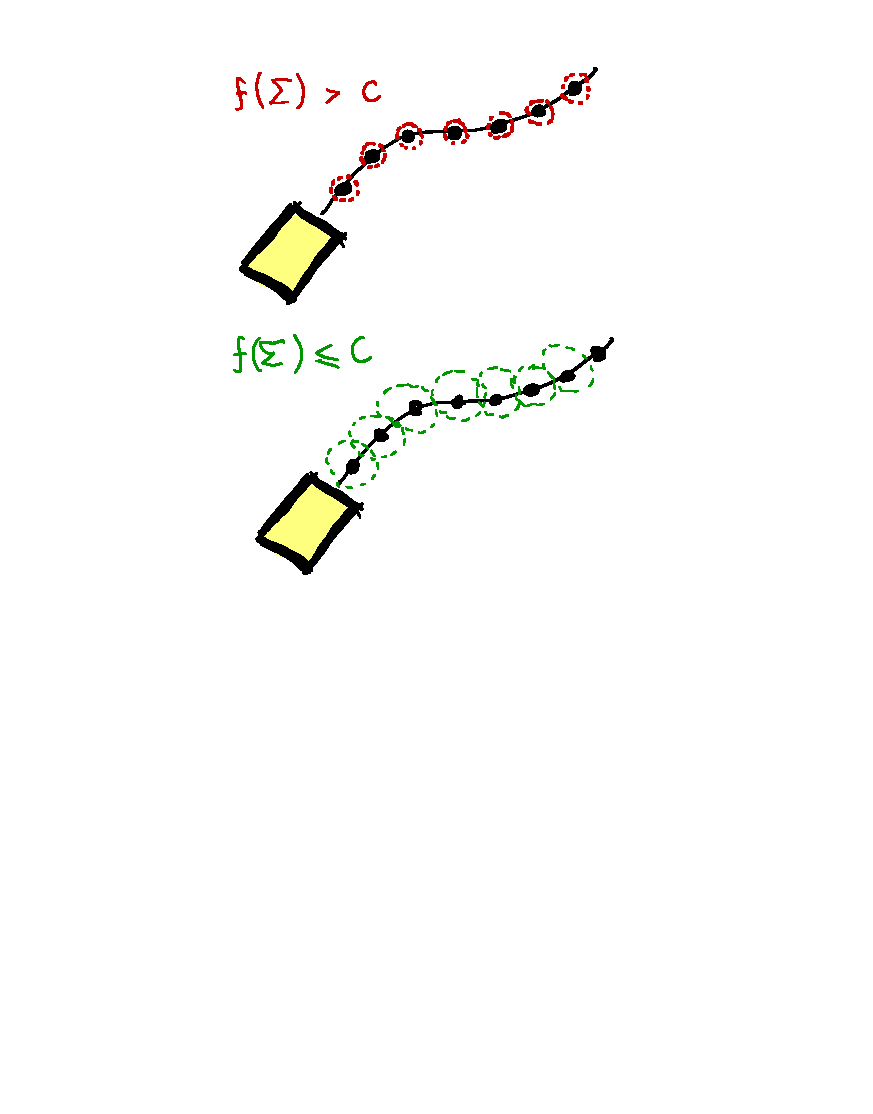
\includegraphics[clip, trim=0cm 8cm 0cm 1cm, width = 0.75\textwidth]{Thing.pdf}
%    \caption{Relaxing the Ridgeback pose constraints depending on the localization covariance, lower covariance gives more space to optimize for manipulability}
%    \label{fig:somthing}
%\end{figure}
\subsection{The SQP algorithm}
Sequential convex optimization optimization can be tackled using sequential quadratic programming (SQP) \citep{schulman2013finding, xu2010two}, a powerful algorithm which repeatedly constructs and minimizes a convex approximation of the problem $\tilde{P}$ until constraints are satisfied.
\paragraph*{Initialize}
The cost and constraint functions can be picked at runtime or compile time.
An advantage of picking the functions at runtime lies in having the ability to parametrized generic versions of commonly used constraints such as collision avoidance or field of view maintenance.
\paragraph*{Convexify}
For each point in the desired trajectory and the penalty value $\mu$, we form convex cost and constraint functions at the operating point.
The cost function is convexified to a second-order approximation while the constraints are linearized at the current configuration.
\paragraph*{Minimize}
The convexified problems are minimized, where the parameter values being considered are subject to the trust region $\delta$.
This prevents the minimization process from taking large steps when the changes in the convex cost and constraint models do not reflect the changes in the non-linear models to a sufficient degree.
\paragraph*{Trust Region}
At each iteration of the innermost for loop, a trust region $\delta$ for the QP problem is updated depending on how well the change proposed by the minimization algorithm translates to the change in non-linear models of the cost and constraint functions.
If the change is deemed sufficient, the step size for the next iteration is increased by modifying the parameter search area of the optimization algorithm.
\paragraph*{Check constraints} 
Once the convexify loop converges (the changes in $q$ become sufficiently small) or reaches a maximum number of iterations, the result is checked against constraints.
If the constraints are satisfied, the algorithm concludes.
Otherwise, the penalty $\mu$ is increased (usually by a degree of magnitude) and the algorithm is repeated.

\begin{algorithm}[h]
 \KwData{$q_{init}\,$}
 \KwResult{Configuration $q$ satisfying $f,g,h$}
 $f,g,h \leftarrow$ Initialize()\tcc*[r]{Initialize problem}
 \For{PenaltyIteration = 1,2,\, \dots}{
  \For{ConvexifyIteration = 1,2,\, \dots}{
  $\tilde{f}, \tilde{g}, \tilde{h} \gets$ Convexify($f,g,h$)\tcc*[r]{convexify problem}
   \For{TrustRegionIteration = 1,2,\, \dots }{
   $\begin{array}{rl} \min\limits_{q} & G(\tilde{f}, \tilde{g}, \tilde{h}) \\
    \mbox{s.t.} & q \in \left[q - \delta, q + \delta \right] \end{array}$\tcc*[r]{minimize}
   \If{TrueImprove / ModelImprove $\ge$ c}{
   $\delta \gets \tau^+ \delta$\tcc*[r]{expand trust region and proceed}
   \textbf{break}\;
   }
   $\delta \gets \tau^- \delta$\tcc*[r]{shrink trust region and repeat}
 }
   \If{Converged()}{
   \textbf{break}\;
   }
 }
  \eIf(\tcc*[h]{Check nonlinear constraints}){$SatisfiesConstraints$}{
 \textbf{return} $q$\;
 }{
 $\mu = k*\mu$\;
 }
 }
 \caption{The SQP algorithm}
 \label{algorithm:sqp}
\end{algorithm}










\chapter{Software architecture}
With the theoretical framework for state estimation and motion planning established in \Cref{chapter:State estimation} and \Cref{chapter:motion planning}, this chapter describes the software implementation of these concepts.
Developing code that is intuitively structured is key in a research context, where it is often maintained and expanded by multiple parties.
Maintaining a heavily tested core code-base which allows modular drop-in components for high level functions can be considered a good development strategy for such cases.
Such a structure expedites testing and data gathering procedures, as it enables quick start-up, user safety and damage prevention.

In \Cref{section:overview} development considerations are explained in more detail and a high-level overview of the software architecture is presented.
Next, in \Cref{section:code state estimation} and \Cref{section:code motion planning} state estimation and motion planning pipelines are detailed.%, focusing on the modularity aspect.
Lastly, \Cref{section:control} describes the control pipeline that relays user commands to the API and internal control loops. %%Due to closed-source control code being used in the robots internally, we omit the details of the algorithms themselves in lieu of explaining interfacing strategies with the low-level APIs.

\section{Overview}\label{section:overview}
Developing software for a complex system such as the Thing mobile manipulator is a time-consuming process, as each change requires extensive testing before it can be applied safely.
Aside from following strict version control methodologies using tools such as \textit{git}, the developer needs to have an idea of what interaction a given change can have with the rest of the architecture. 
It is often inefficient to test every change on the real robot.
Structuring the code in a way that decouples most of the heavily tested core functionalities from specific user tasks is of great importance since it helps the developer maintain an idea of what certain changes can affect.

The testing procedure on the real robot suffers from a high set-up cost, which can be reduced by having start-up procedures stored in the form of ROS\footnote{Robot Operating System - www.ros.org} launch files.
Having a simulation that reasonably models the robots behaviour also expedites testing, as some concepts remain largely unaffected by dynamic effects occurring in reality.
Furthermore, platform-agnostic code is maintained, meaning that the software does not differentiate between the simulated and real systems, drastically reducing implementation time.
\subsection{Architecture}
The network-based nature of ROS systems allows a distributed software architecture.
This enables keeping real-time dependent functionalities on the robot while running high level algorithms on a separate machine.
Specifically, the control algorithms implemented in the \verb|ros_control| interface with the local UR10 and Ridgeback drivers and are ran on the robot's local machine which acts as a server.
Task-specific programs are ran on a separate client machine which connects to the Thing's ROS core via WiFi or ethernet.
\begin{figure}
\includestandalone[width=\textwidth]{slike/software_tikz}
\caption{Overview of the software architecture. White rounded rectangles represent ROS packages, while cross-hatched rectangles represent individual libraries/headers/executables. The dashed rectangles represent the server and client machines.}
\label{fig:overview}
\end{figure} 

\subsubsection{Client}
\Cref{fig:overview} shows how the \verb|thing_control| package forms a robust core of the code-base.
It acts as a central node which processes trajectories and commands sent by the user, which includes:
\begin{itemize}
  \item Receiving and processing data streams from the server
  \item Sending joint angle or position commands to the server
  \item Interacting with motion planning libraries
  \item Monitoring status and implementing security procedures
\end{itemize}
Receiving and sending data is done through the ROS topic interface; subscribers fetch structured data from network locations called topics, which are populated using data publishers.

At compile time, the user can choose a motion planner developed specifically for the Thing mobile manipulator.
These planners inherit from a core part of the codebase, the \verb|thing_kinematics| library.
This library contains the common mathematical framework for the motion planners as well as various useful kinematics functions:
\begin{itemize}
  \item Forward kinematics and Jacobian functions
  \item Pose error calculations
  \item Angle representation conversions
  \item Various matrix operations
\end{itemize}
Keeping this part of code in library form allows for easy transfer of these useful functionalities to other packages.
The motion planners (also referred to as \textit{solvers}) represent different approaches to the problem of solving a given Cartesian trajectory or task.
Both the methods presented in \Cref{section:task priority}, \Cref{section:sqp} are implemented as motion planning libraries.

\subsubsection{Server}
The server maintains the control and estimation pipelines on the robot and takes care of publishing the current state and status to the network.

Direct communication with the base and manipulator is achieved through their respective APIs, but in order to connect these libraries to our networked software structure the \verb|ros_control| package is used. 
It provides a valuable set of tools that abstract the notion of a robot interface and enable quick and easy integration of APIs into ROS-based system architectures.

The transforms representing all of the chains located in the robots URDF\footnote{\textit{Unified Robot Description Format} - Standard file format used for semantic robot descriptions.} file resulting from state estimation are published through the \verb|robot_state_publisher| package. The package publishes the transforms in the form of standardized \verb|\tf| ROS messages.
The package is launched on the robot's local machine since the standardized structure of the control pipeline relies on the transforms published by this package.

\section{State estimation}\label{section:code state estimation}
The EKF algorithm described in \Cref{section:Localization} is available in the \verb|robot_localization| package \citep{MooreStouchKeneralizedEkf2014}.
This package fuses odometry estimates provided by various sources, ideally resulting in a higher-accuracy estimate.
The estimates need to be published to a ROS topic in the form of a \verb|nav_msgs/odometry| message.
Each state estimation node in \verb|robot_localization| begins estimating the vehicle’s state as soon as it receives a single measurement. If there is a holiday in the sensor data (i.e., a long period in which no data is received), the filter will continue to estimate the robot’s state via an internal motion model.

\section{Motion planning}\label{section:code motion planning}
Two motion planning algorithm have been developed, one implementing the \textit{task-priority} (\Cref{section:task priority}) scheme and the other implementing the scheme in \eqref{mnptik_2} via the SQP (\Cref{section:sqp}) algorithm.

Unifying the implementations is a common linear algebra framework, the Eigen3\footnote{http://eigen.tuxfamily.org/index.php?title=Main\_ Page} library.
The Eigen3 library is a powerful linear algebra toolbox capable of handling a vast array of dense and sparse matrix calculations.
It is also templated and heavily optimized for reducing redundant value copying and memory management, making it the basis of many algorithm implementations across a range of fields.

\subsection{Task-priority}
Unlike the SQP implementations, task-priority is implemented using only the Eigen3 and C++ standard libraries.
It relies on \textit{singular value filtering} \eqref{eq:svf} and the \textit{selectively damped least squares} \eqref{eq:sdp} formulation to maintain numeric stability in the pseudoinverse operation.
These functions have been developed from scratch in highly abstracted template form for the purposes of this work.

\subsection{Sequential convex optimization}
Implementation of the sequential convex optimization algorithm is done using Google Ceres\footnote{http://ceres-solver.org/} solver for the underlying convex optimization subprogram.
The objective and convexified constraint functions are implemented as classes in order to be compatible with the solver.
Ceres is configured to run using the Levenberg-Marquardt trust-region strategy with the Broyden–Fletcher–Goldfarb–Shanno algorithm being used to perform line search.

\section{Control}\label{section:control}
The low level control loops of the Thing mobile manipulator rely on the proprietary APIs of both the UR10 and Ridgeback.
Thus, the main challenge of control architecture implementation lies in interfacing with the control inputs and outputs rather than parametrization of a control loop.
The \verb|ros_control| package functions as an integration tool for robot APIs into the networked structure of ROS-based systems.
\begin{figure}
\centering
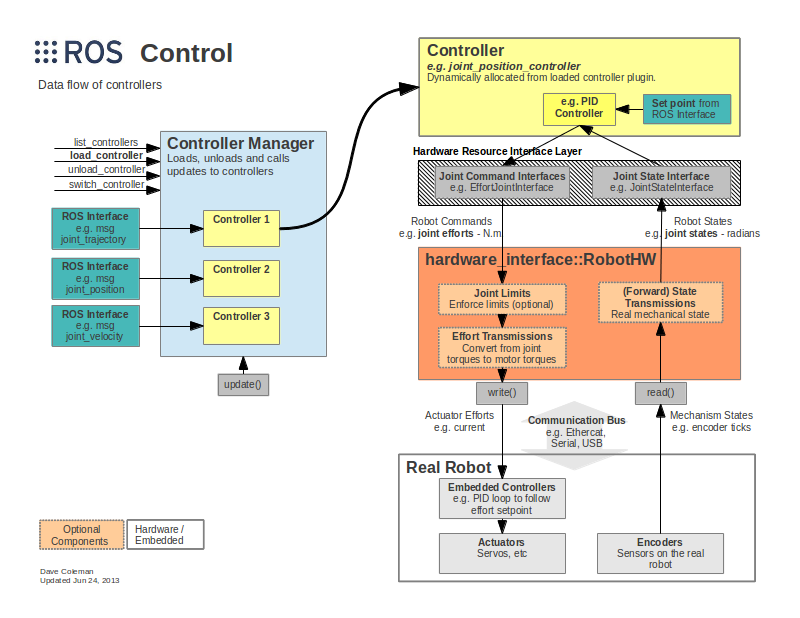
\includegraphics[width=0.9\textwidth]{ros_control}
\caption{Scheme of ros\_ control functionalities}
\label{fig:ros control}
\end{figure}
The \verb|hardware_interface| (\Cref{fig:ros control}) class is used to wrap the read and write methods of the respective APIs in to function handles. 
These handles can then be used by a selection of controllers within the package to either forward commands or implement a control loop.
A ros controller has many types and is configured using a YAML\footnote{YAML Ain't Markup Language - http://yaml.org} file. 
Depending on the interface, this controller will forward commands or actually control the signal using tunable PID parameters.
Additionally, we use joint trajectory controllers which can handle and interpolate multiple timed trajectory points.



\chapter{Experimental results}
This chapter covers the results of the presented state estimation and motion planning approaches.
Since motion planning was considered on a purely kinematic level, it can be extensively tested in both simulation and on the real robot.
State estimation testing proved more difficult as dynamic effects such as slip are not easily simulated.
For this reason state estimation was only explored in data sets collected from the real robot.
\begin{figure*}[h]
    \centering
    \begin{subfigure}[t]{0.45\textwidth}
        \includegraphics[trim={35cm 0cm 0cm 0cm},clip,width=\textwidth]{lidar_test1}
        \caption{Tests in the VICON laboratory}
        \label{figure:VICONtest}
    \end{subfigure}
    \begin{subfigure}[t]{0.45\textwidth}
        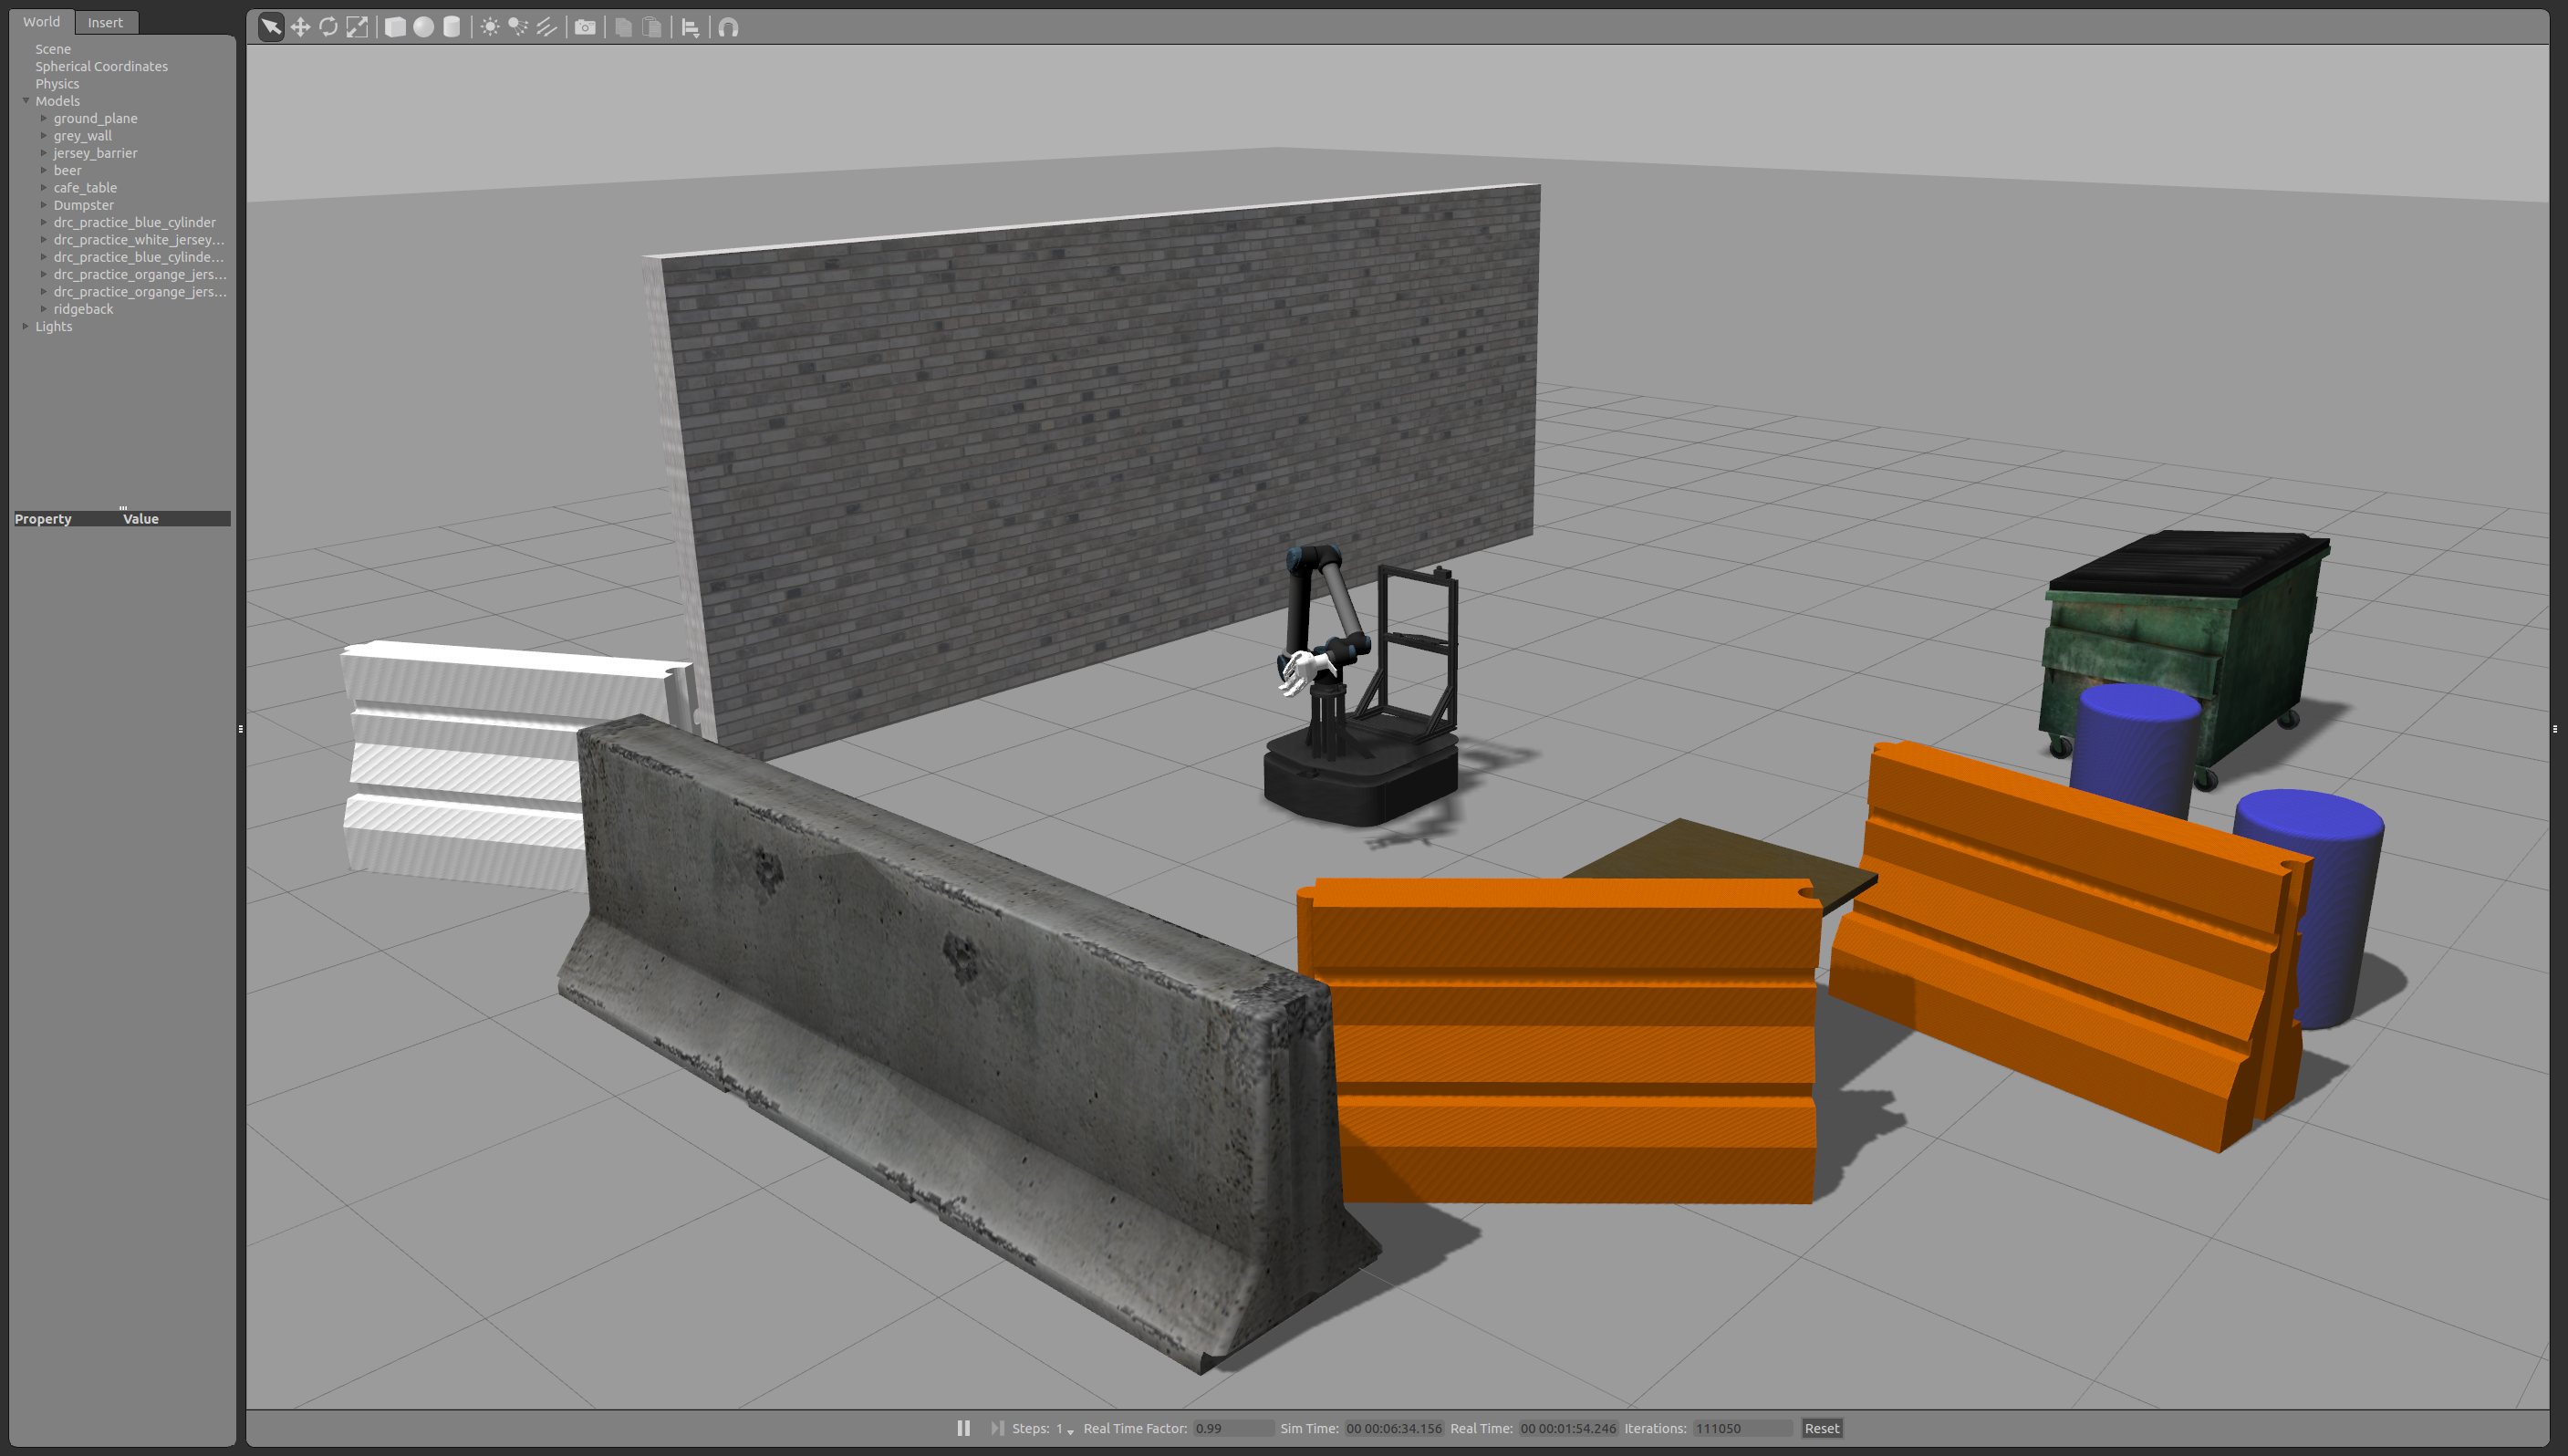
\includegraphics[trim={25cm 2.5cm 10cm 8cm},clip,width=\textwidth]{gazebo_screenshot1}
        \caption{Simulation testing setup}
        \label{figure:simulationtest}
    \end{subfigure}
    \caption{Example of some real and simulated test setups.}\label{fig:resultsphotos}
\end{figure*}
Localization tests were performed in the autonomous robotics laboratory at the University of Toronto Institute for Aerospace Studies (UTIAS).

%The developed software architecture was used for many different applications ranging from Kinect guided servoing to grasp testing.
%However, for the sake of remaining concise only 
Two cases of real robot tests are presented.
The first test focuses on localization, recording the Thing movement under arbitrary user inputs.
The second test consists of performing a set of Cartesian trajectories where the UR10 maintains a straight line while the Ridgeback moves in a sinusoidal fashion.

The Thing mobile manipulator is simulated using the open-source Gazebo simulator.
The main advantage of this simulator is that it is fully integrated within the ROS ecosystem.
Furthermore, the \verb|ros_control| controllers used on the actual robot are also used in the Gazebo simulation, making interfacing identical to the real robots.
Other sensors such as LIDAR can also be simulated with a configurable amount and characteristic of noise.

\section{Localization}
\Cref{fig:ekf_localization} shows the results of base localization on a dataset consisting of manual Ridgeback movement inputs.
Two variants are compared: the first variant  uses an EKF to achieve fusion of both the wheel and LIDAR odometry, the second variant integrates wheel odometry alone using the EKF only to account for measurement noise.
Ground truth was established using the VICON motion capture system, which provides sub-millimetre level accuracy.
VICON\footnote{https://www.vicon.com/} is a commercial motion capture system often used for the purpose of setting ground-truth values for state estimation tests. 
\begin{figure}[h]
\centering
% This file was created by matlab2tikz.
%
%The latest updates can be retrieved from
%  http://www.mathworks.com/matlabcentral/fileexchange/22022-matlab2tikz-matlab2tikz
%where you can also make suggestions and rate matlab2tikz.
%
\definecolor{mycolor1}{RGB}{ 38, 166, 91}%
\definecolor{mycolor2}{rgb}{0.85000,0.32500,0.09800}%
\definecolor{mycolor3}{RGB}{75, 119, 190}%
%
\begin{tikzpicture}

\begin{axis}[%
width=4.682in,
height=3.6in,
at={(0.785in,0.486in)},
scale only axis,
xmin=-0.5,
xmax=1,
xlabel style={font=\color{white!15!black}},
xlabel={x [m]},
ymin=-0.2,
ymax=1.4,
ylabel style={font=\color{white!15!black}},
ylabel={y [m]},
axis background/.style={fill=white},
%title style={font=\bfseries},
%title={EKF odometry},
axis x line*=bottom,
axis y line*=left,
xmajorgrids,
ymajorgrids,
zmajorgrids,
legend style={at={(0.156,0.779)}, anchor=south west, legend cell align=left, align=left, draw=white!15!black}
]
\addplot [color=mycolor1,line width=1pt]
  table[row sep=crcr]{%
6.28612846153842e-05	2.51965475542154e-05\\
9.77225408177462e-05	-4.01509786358833e-05\\
7.62616093439306e-05	0.000178726628546844\\
4.89661012158527e-05	0.000150750214168827\\
5.47246500886486e-05	0.000255191013130276\\
0.000104783497418263	0.000142188469222759\\
4.19614936356394e-05	0.000118277191405725\\
0.000162329007018028	0.000130311228559624\\
-3.10309197674163e-05	0.000242354947985898\\
0.000185622277808641	5.24663669910774e-05\\
2.81565392624208e-05	4.14027649921628e-05\\
-5.74593650044114e-05	4.24448394022031e-05\\
0.000144371103512564	5.89668849284991e-05\\
7.49571222413564e-05	2.08701473315559e-05\\
-4.72816011319044e-05	6.19806260526989e-05\\
0.000181988585342019	0.000103724692286838\\
0.000261095932502974	0.000205889236927922\\
0.000224283039116584	3.22314725013928e-05\\
6.67830391812563e-05	0.000188861252775091\\
-1.11410436451076e-05	9.8063689583136e-05\\
4.43446249952101e-05	0.000173698551394874\\
0.000151461057912715	1.57223867234962e-05\\
0.000142278028875446	5.76500301022187e-06\\
6.41867484418163e-06	4.56375516730417e-05\\
-2.6571682340687e-06	0.000124330662335012\\
0.000119134311348884	-6.38456661988807e-06\\
4.66601860236518e-05	8.84011674792268e-05\\
0.000231719014463221	-2.30754518951853e-05\\
6.65146661682839e-05	9.17372675138112e-05\\
0.000134330992549003	0.000104930983901644\\
0.000382238938425219	0.000306891615147326\\
0.000326967238680267	0.000318339466775744\\
0.000183388045270405	-2.87879080084902e-05\\
5.11818577334511e-05	0.000182742227525068\\
-8.36664870218079e-05	-2.37427709747218e-05\\
0.000205209872296878	8.66704182442418e-05\\
8.04156316759758e-05	0.000168942249172202\\
9.44069841287143e-05	-3.10635113244667e-05\\
0.000220786733376263	5.80449024394636e-05\\
0.000124030199634945	0.00011300711365296\\
0.00017132949968101	1.5434922280011e-06\\
0.000148671201525542	1.42399322252407e-05\\
0.000112275595636216	0.000152815832092201\\
0.000219006178388298	0.000334346698493776\\
0.00014265948688872	0.000127364052676798\\
0.000221768792342064	6.75067216399372e-05\\
4.01303536616271e-05	-8.34901528188603e-05\\
0.000259976569730348	0.000268255120615415\\
0.00021409894653298	4.81556634950447e-05\\
7.44519193913856e-05	-4.46168998019386e-05\\
3.92459505209192e-05	1.70492931452909e-05\\
0.0002661073566739	0.000148951107085293\\
5.67945216248117e-05	6.4491215300333e-05\\
3.09826222526927e-06	2.93349529227743e-05\\
0.000289728430289668	0.0001763313082455\\
0.000243114697029402	0.000395805360883461\\
8.5416146125783e-05	1.16630821021813e-06\\
0.000258814208288105	0.000168569948764727\\
0.000201431214361725	-5.20678231839822e-05\\
0.000100855307859832	0.000203797129412445\\
0.00017097473094458	2.01616696676732e-06\\
0.000290552198555553	0.000125288183253733\\
0.000277693047563546	0.000147905668627699\\
7.94981380952131e-05	0.00028708544150205\\
3.92327491470987e-05	0.000211183852324021\\
0.000291049824429783	7.38167974749931e-05\\
0.00109654124687748	-4.93013868643616e-05\\
0.0028660817437496	-0.000450469199983969\\
0.00714765543668146	-0.000666093254271277\\
0.0128116852730542	-0.0012495525158881\\
0.018447610864353	-0.00173587459017455\\
0.0215103988082662	-0.00193883318969383\\
0.0243886881786806	-0.00201261076049843\\
0.0309046261856262	-0.00293531001783399\\
0.0439019670059303	-0.00463928200667788\\
0.0493055712800541	-0.00509473904217238\\
0.0545511478563844	-0.00555474185610454\\
0.0592906074463817	-0.00548063919813373\\
0.0652461426101595	-0.00650205738428725\\
0.0746681023916896	-0.00727582762807115\\
0.0798863859000749	-0.00762279626649828\\
0.0898239396196476	-0.00902578000469702\\
0.0998993162370925	-0.00976308063195513\\
0.105342295247501	-0.0104104890560966\\
0.110527342507382	-0.010888990520354\\
0.131413636661927	-0.0128943089740079\\
0.138602734121672	-0.0136133475007029\\
0.147371925939373	-0.0148915994555338\\
0.163990256367886	-0.0166907805032064\\
0.1785072158231	-0.0178054257668784\\
0.185865128419791	-0.0182707603328307\\
0.193277502870887	-0.0193694114311594\\
0.207853444279779	-0.0210236428110017\\
0.222610314465006	-0.0223997407193949\\
0.229889568458062	-0.0238343127918324\\
0.239550974364359	-0.0240518740869544\\
0.267957941195967	-0.0276395128367998\\
0.27586049590226	-0.0282516994079154\\
0.283151956721414	-0.0290681639273232\\
0.297519205341832	-0.029928943875495\\
0.312832253540154	-0.0311612088270239\\
0.32103933687439	-0.0319173728600923\\
0.328693927573642	-0.0326960262450458\\
0.356356339077932	-0.0354861676591697\\
0.36020379298985	-0.0353404745629102\\
0.360162218620425	-0.0350927649959414\\
0.359240938286625	-0.0350152329292208\\
0.358460635527793	-0.0349008360095523\\
0.358112211121691	-0.034644715908509\\
0.357291788732297	-0.0349220991591322\\
0.352207838088347	-0.0342737368346668\\
0.33866589131342	-0.032586947064796\\
0.334435300452298	-0.0320559708667695\\
0.320877521661443	-0.0310089745152508\\
0.317583560038716	-0.0304811937542549\\
0.314275344007809	-0.03074943039832\\
0.311107024260542	-0.0297976220802226\\
0.307461897951356	-0.0295897798820561\\
0.298834574841521	-0.0288914148057989\\
0.295089517818131	-0.0281766620032286\\
0.291121358656109	-0.0279271158743403\\
0.279558569534313	-0.0264942292772195\\
0.276311341491443	-0.0262351450781735\\
0.26932155982021	-0.025821885498458\\
0.265620394528363	-0.0260296162609331\\
0.262195222216112	-0.0260399540571\\
0.253549089256167	-0.0255310621543474\\
0.248978688040166	-0.0258274022503611\\
0.24513023689414	-0.0250788872342128\\
0.241433809968211	-0.024133512155674\\
0.238698868964991	-0.0236696535001846\\
0.227895000481366	-0.0242525325962365\\
0.225195862310723	-0.0236003909046234\\
0.22637950338847	-0.0233671157051121\\
0.229077867295791	-0.0224954008282634\\
0.231943944475836	-0.0231676798448991\\
0.236324184839091	-0.0237314395796132\\
0.246690837095513	-0.0232244652079742\\
0.262048043659934	-0.0223356464207201\\
0.271301131123779	-0.022369245767995\\
0.2808919474571	-0.0222727945603568\\
0.297833229831412	-0.0224890164830636\\
0.313130648247603	-0.0230117188701593\\
0.32137902332886	-0.0237865270945227\\
0.329830909730791	-0.0249795658017836\\
0.345872263597224	-0.0266158989637058\\
0.361507961772114	-0.0299681026760141\\
0.36946095242451	-0.0327796677923437\\
0.377587663003732	-0.0354875505367323\\
0.393797896540926	-0.0402154516007968\\
0.406935153235934	-0.0449893519634026\\
0.410238298345305	-0.0449570398539046\\
0.40894470246925	-0.0440762247676562\\
0.407126949216951	-0.0431884667064523\\
0.405726931837354	-0.0436401493665594\\
0.405648540746113	-0.0430022632449594\\
0.401941474796102	-0.0414930351491914\\
0.392718277100795	-0.0395884066657712\\
0.384890596796872	-0.0380881501856113\\
0.381399408212141	-0.0361711680517003\\
0.377450826221075	-0.0347018499647272\\
0.367941583233143	-0.0324685663696388\\
0.352469610245219	-0.029543472554611\\
0.347075632549718	-0.0294527935420321\\
0.341013510038627	-0.0288372577087528\\
0.327972180272092	-0.0276152838628177\\
0.316821053495755	-0.0265702707342032\\
0.310032701296529	-0.025700078513333\\
0.303834130356767	-0.0256107452961515\\
0.297446144943135	-0.0250389112475715\\
0.291713905049783	-0.024974309070454\\
0.279565072590215	-0.0246595304191865\\
0.273709127950952	-0.0247580700960197\\
0.267203905257143	-0.0251931483264937\\
0.254271353075818	-0.0259386010769646\\
0.246859691243217	-0.0266919727070054\\
0.240808742577596	-0.0277062249323859\\
0.236466423098962	-0.0281944557156626\\
0.229938689987002	-0.0296395612056711\\
0.22361288131531	-0.0304270145925235\\
0.218172840477181	-0.0316256876050436\\
0.206506394025418	-0.0338384987830647\\
0.200835736950277	-0.0350608924653358\\
0.195169462599472	-0.0365117532473909\\
0.186792382354045	-0.038597583023121\\
0.187703425812109	-0.0379724139278065\\
0.188679983855162	-0.0367769529366585\\
0.189840149287617	-0.0361374939021684\\
0.193900123973449	-0.0368446681294739\\
0.210018637310082	-0.0352460320390588\\
0.219857084123977	-0.0332009128044669\\
0.23125986974507	-0.0310327276385177\\
0.265045725003034	-0.0231639484095168\\
0.275271395154172	-0.020015203333321\\
0.286770242090854	-0.0171560559261165\\
0.298071082343279	-0.0155909216032843\\
0.319456960123189	-0.0104137755773667\\
0.340457965234237	-0.00637518302732999\\
0.352116187803144	-0.00415237290182999\\
0.363077615886327	-0.00167934742893039\\
0.384615488624157	0.00291597376550863\\
0.406072441799826	0.00742843364762424\\
0.417477903560681	0.00956632047031451\\
0.428608089639532	0.0114030551637584\\
0.439326701666296	0.0141632696796062\\
0.44968512246443	0.0161802196041737\\
0.462239226250103	0.0186071972435935\\
0.471706195147192	0.0202666192225452\\
0.482588144788082	0.0226068671179561\\
0.493757878500598	0.0248383283056608\\
0.536476194225572	0.0336449299069055\\
0.547398506574837	0.03573342605077\\
0.558816118638957	0.0381115726436542\\
0.57005936454958	0.0401014676782034\\
0.58016814110501	0.0426950869239881\\
0.599648351283727	0.0466631942568587\\
0.605600122065452	0.047573026972397\\
0.608399687109754	0.0481131121783425\\
0.608928213522907	0.0488031995320393\\
0.60757436763463	0.04840225450788\\
0.60367486176951	0.0473999614973968\\
0.59685136143639	0.0456180849302568\\
0.589270185933453	0.04401795183525\\
0.582386227898013	0.0424577686920418\\
0.567695788384921	0.0398719247574827\\
0.5594586508613	0.0385499406565191\\
0.550570494561758	0.036775138066565\\
0.534216000928696	0.033262240799959\\
0.518431824563679	0.0301055218641736\\
0.508500490234295	0.0284370160566602\\
0.497180601989359	0.0264897930418665\\
0.473063667859536	0.0214339209623675\\
0.452193185077296	0.016964629862161\\
0.440935172694454	0.0152752915424393\\
0.427279580208734	0.0121574268813027\\
0.407738447882077	0.00799450799212892\\
0.386202038157625	0.0022441404867888\\
0.375119321961986	-0.00162243065568789\\
0.364601827476025	-0.00600965549602994\\
0.344607618898676	-0.013961899886629\\
0.31247624898362	-0.0249739620087866\\
0.301869902487713	-0.0304988658797771\\
0.261869663051136	-0.0478502631773903\\
0.251111877461805	-0.0528539753870355\\
0.240861121727573	-0.0591498222491548\\
0.208795250233301	-0.0771424515886309\\
0.205046251924917	-0.0787427683394001\\
0.203029288370556	-0.0803711310296449\\
0.201744913628055	-0.0812423529269169\\
0.201732988976083	-0.0815073845319842\\
0.20254438374038	-0.0815163533688026\\
0.206757629342819	-0.0793349176747538\\
0.214638257467618	-0.0751344331904739\\
0.233453614910614	-0.0657630005716207\\
0.252365251857677	-0.0579497369453807\\
0.266100100346191	-0.0513929255375459\\
0.279441438892766	-0.0431386400143316\\
0.292285259533821	-0.034883610603373\\
0.303361930907021	-0.0268104521055046\\
0.327570289707603	-0.012761669490324\\
0.340705802806785	-0.00552900780706243\\
0.353366541770234	0.00218343383246282\\
0.377240226625216	0.0160117818501072\\
0.402116098333506	0.0313270819578191\\
0.415012298844453	0.0381769701523994\\
0.427812686264559	0.0458449177157612\\
0.451601615646894	0.0605007622732265\\
0.474241270700103	0.0780156589614603\\
0.48634427639943	0.0877896375682028\\
0.498297646930422	0.0991226750207532\\
0.520253088325356	0.120462445345808\\
0.538026045702565	0.146648638254801\\
0.546679104556991	0.160366114374255\\
0.553793420888135	0.176082833982487\\
0.558896883378101	0.19437644205407\\
0.561719824884966	0.210807647861799\\
0.5613404057467	0.242659708179781\\
0.556975664223858	0.259145087182495\\
0.534481449714663	0.294080894166124\\
0.515216802415398	0.31872500592624\\
0.504243060249819	0.332867320792247\\
0.493363224044649	0.345718737229108\\
0.47112983821364	0.371358096614544\\
0.445692664045159	0.393226859769715\\
0.430196532841266	0.40519852434241\\
0.414926710123225	0.41550738158004\\
0.398949092484096	0.425050993037819\\
0.382947864493969	0.432246302899374\\
0.347350221983722	0.443933998236706\\
0.328447176297426	0.449329491908315\\
0.308919455818869	0.449887999333952\\
0.289182534513868	0.450094304854\\
0.271526973101733	0.449050011023202\\
0.237253379943222	0.440558404383752\\
0.222197908678727	0.432701171070578\\
0.209358593051554	0.423175118923385\\
0.197292819252611	0.412829022255704\\
0.185024096724126	0.402045782739784\\
0.172903762450214	0.390677880981997\\
0.156332379654119	0.37615694998703\\
0.143427039321521	0.365451326062312\\
0.128581893979577	0.353755781713909\\
0.113236586746203	0.3396210760672\\
0.092194370851399	0.316410918330267\\
0.08246617831848	0.302967174077119\\
0.0732899790504377	0.289967159661492\\
0.0625982360922262	0.262773241903605\\
0.0578691847010801	0.239602589792886\\
0.0570460615326268	0.226362201758653\\
0.0557461385945047	0.213368868527498\\
0.0547557201283617	0.201296554279208\\
0.0541826914491287	0.189466175304412\\
0.0555218694432463	0.164871034835694\\
0.0583685066584095	0.152337439572136\\
0.061760500743243	0.138656484276776\\
0.0661100701608938	0.125300898775631\\
0.0837545077325915	0.0899233878360403\\
0.0905418117374267	0.0779254985138805\\
0.0990027515275739	0.0670303229920266\\
0.135465842265411	0.0220960232980478\\
0.14564758921688	0.00998428622958096\\
0.15623621535537	-0.00167920349321957\\
0.178355809522777	-0.0210007125916101\\
0.201688283235066	-0.0399826588605275\\
0.214994124302581	-0.0502198647159798\\
0.228661815801369	-0.0602431525665456\\
0.242858351602362	-0.0689919980488917\\
0.285788443371086	-0.0907192041316134\\
0.301049084195734	-0.0981703783109016\\
0.317109453273701	-0.104620042988576\\
0.350434338556555	-0.110069194434453\\
0.384617076469293	-0.110134234782541\\
0.402835287696119	-0.10714583474708\\
0.421729364712543	-0.103633465678308\\
0.456971500651055	-0.0939392369232507\\
0.509376728297224	-0.0790874541215075\\
0.526252158263983	-0.0733957198028448\\
0.556423823139245	-0.0603906553207223\\
0.58290220742624	-0.0415540654393802\\
0.596172865018205	-0.0307376641879164\\
0.60880670294225	-0.019017129910826\\
0.633858128852045	0.00289549733864977\\
0.64820251167613	0.0138817194925842\\
0.664340819228773	0.0277156337744768\\
0.675607314622549	0.035638429843983\\
0.68093531483628	0.0407031324251546\\
0.681340288971894	0.0500351739916962\\
0.67385748537082	0.0690195998095713\\
0.676693857634549	0.0783432193465287\\
0.680655541027124	0.0887040923352886\\
0.689159415829528	0.10839129836273\\
0.699036705007335	0.126466100797437\\
0.703806833000244	0.136376173655932\\
0.708446607181879	0.145973098658979\\
0.71758479742707	0.169685143079779\\
0.729583172209113	0.199130705828507\\
0.736234826815132	0.216053147500418\\
0.742268998132153	0.231681247407795\\
0.748051062973183	0.24832280211672\\
0.757395963806358	0.29585932708008\\
0.755539393611962	0.313434512629075\\
0.739545315585099	0.365733828984034\\
0.724467181853898	0.398427639952821\\
0.715336652951402	0.414444688344442\\
0.705475243412554	0.428933257282315\\
0.683286841371614	0.453956397872347\\
0.656177326864914	0.475405904644563\\
0.639954982420856	0.485262196881063\\
0.624126738177618	0.493979245628493\\
0.593677645932786	0.511227480142502\\
0.563863955527843	0.529942184904435\\
0.548533471525985	0.53989361683683\\
0.532555139509129	0.549638403913495\\
0.516681257535581	0.559178497918375\\
0.50226900030574	0.568940086797693\\
0.456850094680992	0.59695006698559\\
0.439177184170091	0.606174980053272\\
0.403916662389391	0.615192159565907\\
0.36815407036772	0.614464568505232\\
0.350682910985651	0.609891011700076\\
0.334738589989116	0.603287243152323\\
0.318773324040274	0.596380154666604\\
0.304082665449876	0.591259586688075\\
0.275356365867807	0.571777653479648\\
0.262015562584946	0.559848811336779\\
0.248850163581698	0.547218526184512\\
0.221102185640807	0.51712758442835\\
0.203222005920541	0.494695171439548\\
0.192285252874094	0.48009788301931\\
0.18321887682852	0.462199471463191\\
0.168929079428955	0.426740915122156\\
0.157056934160513	0.387769710082362\\
0.151532498513112	0.366802297682438\\
0.14607057182678	0.344319378649408\\
0.135291447658248	0.303928787659297\\
0.120461688675172	0.244003963274651\\
0.115024670550702	0.223737087444704\\
0.103498280590888	0.184319162212474\\
0.0915581537735694	0.146023275891418\\
0.0839419695314668	0.120872776827456\\
0.0785155555511597	0.105433212462887\\
0.0670573247488072	0.0679190703794076\\
0.0604424161773288	0.0348024012820389\\
0.0594835412510319	0.0200176714095271\\
0.0609905809778125	0.00635666543518013\\
0.0937571065139277	-0.035831455061472\\
0.108209981775033	-0.0460982849589981\\
0.123299160331522	-0.0561288890874564\\
0.157029780699598	-0.0719686085870865\\
0.194632031409641	-0.080701335546497\\
0.215973751933634	-0.0830599354811917\\
0.236032014103148	-0.0850561346924013\\
0.273466371516483	-0.0913705135254235\\
0.32953163789238	-0.101192208666506\\
0.349096364335847	-0.102885929242368\\
0.384942597589393	-0.108326096226094\\
0.420727481979765	-0.114005829174487\\
0.43984489675921	-0.118000901280031\\
0.458447410403415	-0.121366432108583\\
0.493047183004798	-0.126229393768772\\
0.545682457801335	-0.126219886155825\\
0.56382330831093	-0.124091243489717\\
0.598165522428741	-0.118140181039471\\
0.63185724356535	-0.105351316185889\\
0.649021001196347	-0.0958938394822101\\
0.663300941629587	-0.0852000506036881\\
0.678986429126395	-0.0642885261892824\\
0.685077790359855	-0.0389017968744044\\
0.688141698754004	-0.0240544695512933\\
0.69206631157834	-0.00918446634039101\\
0.696319622577628	0.00602067191501135\\
0.699764477957931	0.020588726958475\\
0.707176832561674	0.0505820222102212\\
0.711748861390417	0.0663164531114992\\
0.716094448772355	0.0817840086845452\\
0.725057226280493	0.109703448045825\\
0.733460107675357	0.139088891366235\\
0.736931864100973	0.155445230837888\\
0.740366919721991	0.17305518513513\\
0.748187888072442	0.205720667839059\\
0.757095100410827	0.238273426279905\\
0.762068967107072	0.255923028345193\\
0.766935836940054	0.273069672256073\\
0.776515166770155	0.305018802123397\\
0.787540188506515	0.336950868169015\\
0.79329149249912	0.353604225907223\\
0.799746426082103	0.370639043588076\\
0.804393168929195	0.387546463444441\\
0.808744337246589	0.40272234538322\\
0.818972115636513	0.434616531669944\\
0.83005097538382	0.468341202106197\\
0.841179575822202	0.499859733460238\\
0.853263129145776	0.531204122939196\\
0.859739429316205	0.547658713698133\\
0.866507930807621	0.563911995897395\\
0.878712365532215	0.593926451302149\\
0.889273945254113	0.626249060558344\\
0.894070540644891	0.642788367101886\\
0.899379204733247	0.660057490391776\\
0.891890822972882	0.731171453209521\\
0.882882014447169	0.749241617335719\\
0.873343747662604	0.766734584028801\\
0.863843443666778	0.784281529581533\\
0.854953040815281	0.79928644963528\\
0.836476375887513	0.831291767601515\\
0.827176702620739	0.84864764955487\\
0.817861030536733	0.866530661215824\\
0.800537626448714	0.900138510871834\\
0.783003536505373	0.932794051997179\\
0.773848500764036	0.950411354283741\\
0.764749350034612	0.967855249367207\\
0.729820531498434	1.03357407087732\\
0.720608026756842	1.05110318626157\\
0.711325984264934	1.06816534454777\\
0.70211735689565	1.08539659017289\\
0.676082160366833	1.13520255295336\\
0.668057519439708	1.15045744706749\\
0.659065756820485	1.16742383866162\\
0.641897319511678	1.2002266743653\\
0.625108074727974	1.23282008512337\\
0.616185705213215	1.24905104688901\\
0.609381407921154	1.2621021191838\\
0.605234315256755	1.27046086521171\\
0.604838323587375	1.27313128445863\\
0.605317236814657	1.27381385655186\\
0.605181450559572	1.27199220138264\\
0.604982540418936	1.27081806548229\\
0.605450379268485	1.27078227935926\\
0.605125923992745	1.27081380451842\\
0.605189456543017	1.26843714373721\\
0.604361635490643	1.2649042710951\\
0.601804551357506	1.25617295669274\\
0.598709918780368	1.24588029066024\\
0.59706120656712	1.23965919871265\\
0.59492787139856	1.23223872377962\\
0.5928334901129	1.22535785149654\\
0.585696161910123	1.20320616505038\\
0.583395631365979	1.19540917528686\\
0.581122691696816	1.18760893331961\\
0.578830015867391	1.17881500115355\\
0.575672984290804	1.16806746202327\\
0.56911509557275	1.14683510269779\\
0.56492147912936	1.13379366152206\\
0.561366762425497	1.12080624483059\\
0.553884774677183	1.09625625506817\\
0.547124071418035	1.07231487737956\\
0.543237625420905	1.05866128060988\\
0.539772232761728	1.04470989383328\\
0.536379744363877	1.03115274967145\\
0.533722967821789	1.01972157308084\\
0.525578319965435	0.981512524246738\\
0.522577768914539	0.967440233401381\\
0.518716213589979	0.929360789314369\\
0.517793571956692	0.914841763940563\\
0.516816810538853	0.902055210478377\\
0.515854118630272	0.888639965043342\\
0.514240028114871	0.862400835586866\\
0.511601954680845	0.835946012052424\\
0.50993392378703	0.82195540307504\\
0.507631371083212	0.808753356916082\\
0.505690150922295	0.795568967699313\\
0.503786619891275	0.783483267497861\\
0.498928562404068	0.757862693450959\\
0.495889742774792	0.744474138457505\\
0.492630635102356	0.730667886731142\\
0.485662023362783	0.705147602947678\\
0.48133578454624	0.690723573240801\\
0.473066781597308	0.665578687882607\\
0.469109517771838	0.654215786436894\\
0.464108922554813	0.641350695680243\\
0.459457305438312	0.630258070733884\\
0.448671082805414	0.607550712966106\\
0.442603951970896	0.596755326381554\\
0.436962713014918	0.587822535495739\\
0.428220710269769	0.578311218286561\\
0.425185428750027	0.574642482751494\\
0.422550173950022	0.57100560481944\\
0.419401341037301	0.568114470189307\\
0.415465712568755	0.564183248770721\\
0.411798932926124	0.559558233231147\\
0.402812049764766	0.542131404639191\\
0.400694329593614	0.53595956664981\\
0.400481254474305	0.532242865648462\\
0.401155849342361	0.530549983590573\\
0.402075940578615	0.529278888366043\\
0.40614830431543	0.528562502794009\\
0.407683462676965	0.527817499759717\\
0.409293816697149	0.527049716492681\\
0.415532405527693	0.52267526774414\\
0.433961989162458	0.517797399153544\\
0.464269436731159	0.522201189846225\\
0.520952118815609	0.539280400351201\\
0.533844711678061	0.544468734896472\\
0.544721673813888	0.550185980331947\\
0.556433034135928	0.563782472948827\\
0.563906279649229	0.590877589736914\\
0.56415305420153	0.601233464184468\\
0.564219821058095	0.620956633531273\\
0.5596835018705	0.644199741018544\\
0.554393310173065	0.656098996945924\\
0.546716799440354	0.666959803073887\\
0.531237545388558	0.688552953949212\\
0.513643547628969	0.706045496860537\\
0.502495484520611	0.713110781191887\\
0.489511504932351	0.718571155848731\\
0.43649371264111	0.729769708828797\\
0.422700604467714	0.730982972110195\\
0.409098809570474	0.733242403455476\\
0.394388286624475	0.734813451887431\\
0.381786499441922	0.735825014014498\\
0.35578733414955	0.737620112854436\\
0.341568036510429	0.737818000934942\\
0.32754845282808	0.737911862457832\\
0.301625382438595	0.737339419665682\\
0.259674400020074	0.735280003934151\\
0.245259267680657	0.733866024490798\\
0.188265375031551	0.724545970035058\\
0.172653730644891	0.721563403255129\\
0.157199244261477	0.718258895094629\\
0.128051558673005	0.712830725385933\\
0.114889578929251	0.710120640257625\\
0.100034293870594	0.707024100399014\\
0.0845933916129405	0.703097409932887\\
0.0687522617325256	0.699327590046349\\
0.0391652453745106	0.691670436691776\\
0.00825983511302837	0.683985419041257\\
-0.00552946483634788	0.680361330652638\\
-0.0213234328681754	0.676226195692358\\
-0.0369060161743291	0.672325768121802\\
-0.0507000067637324	0.668311439891372\\
-0.0662620284729349	0.66428493017971\\
-0.0800203109109617	0.659827856249162\\
-0.0954867610298954	0.655628604142909\\
-0.110727217332444	0.650786808402458\\
-0.139837207028407	0.641654844270877\\
-0.168598664019576	0.632164779317156\\
-0.183954157577794	0.627385587482969\\
-0.199020538716856	0.622200998843638\\
-0.256558551424748	0.603597385977375\\
-0.271747261314123	0.598691212118681\\
-0.287230456045608	0.5939972248601\\
-0.344878689921999	0.575023318153748\\
-0.360384623991989	0.569843756333745\\
-0.375207742754786	0.56541126801335\\
-0.402399199378869	0.555994152620247\\
-0.428483476394759	0.547630859655561\\
-0.440781201658335	0.543365951518403\\
-0.448186840816224	0.540232354410894\\
-0.451222051017898	0.539680948282534\\
-0.450798969810301	0.539793407934621\\
-0.45007559594859	0.540191724719203\\
-0.44947789250386	0.539995839677654\\
-0.448800683662256	0.540046627323954\\
-0.435694447138457	0.545836443840785\\
-0.413723567287576	0.554657631716801\\
-0.401461066036831	0.56002150784318\\
-0.389666125552482	0.564340142937613\\
-0.347298609454773	0.577753522943437\\
-0.335839267983358	0.581797238414146\\
-0.323805775396563	0.585251444697385\\
-0.278646625403388	0.596669175322448\\
-0.267512517361622	0.599680917048543\\
-0.256221530333625	0.603270960682459\\
-0.235885950090206	0.611020520453392\\
-0.204427578566732	0.621356965056162\\
-0.19332965310773	0.624670621842476\\
-0.172659093844248	0.63206951961549\\
-0.153152268267175	0.64045743998454\\
-0.142650903441352	0.644846047688486\\
-0.132652532308634	0.649541526222449\\
-0.113556725833616	0.659019287877015\\
-0.0943197746951488	0.668929933326587\\
-0.0848626012386164	0.674558615662379\\
-0.0783059991580794	0.678830745555852\\
-0.0772828909124928	0.677458683954466\\
-0.0802918897429675	0.675345621244211\\
-0.0799054805377853	0.6770073547276\\
-0.0792526327632425	0.677584882763582\\
-0.078350176521319	0.677494924282652\\
-0.0783332447165719	0.677402621311627\\
-0.0783795385726993	0.677433203206849\\
-0.0783601843288821	0.677541071658168\\
-0.0788375089050447	0.677305808802063\\
-0.0787048953700905	0.677323083029225\\
-0.0788241859845144	0.677157628596025\\
-0.0786362700732006	0.677253664193303\\
-0.078608381731392	0.677186195762411\\
-0.078710820661994	0.677134132052638\\
-0.0787955951107194	0.677109228069834\\
-0.0784846003252062	0.677407331725955\\
-0.0786739472454718	0.677181616576669\\
-0.0787490997334515	0.677107655047036\\
-0.0787557868206546	0.677057657786571\\
-0.0786614435446224	0.677113253935402\\
-0.0784819211086613	0.677240033531485\\
-0.0788048031386305	0.67708398258824\\
-0.0789820753806595	0.676951917186423\\
-0.0787405821101106	0.677087272192247\\
-0.0787022612156907	0.677135942401276\\
-0.0786845916104833	0.677266634883926\\
-0.079170136091374	0.676890956241635\\
-0.0785302046625269	0.677259052028825\\
-0.0785373829514164	0.677164276219582\\
-0.0786431834098641	0.67727578500625\\
-0.0787238249125267	0.677102878099133\\
-0.0786081873678274	0.677200014218428\\
-0.0787106969756212	0.67705397947044\\
-0.0785569612896544	0.677270692295153\\
-0.0783640884649641	0.677374314164766\\
-0.0785807006031921	0.677195295607327\\
-0.0787236866260353	0.677113666124526\\
-0.0785861440280686	0.677188009502713\\
-0.0786939386419647	0.677253572695628\\
-0.0785486608054548	0.677220275023\\
-0.0786499274507412	0.67719102868193\\
-0.0785045650311178	0.677291492023546\\
-0.0786812306811794	0.677215027166863\\
-0.0786648436855314	0.677186200900966\\
-0.0786343672189499	0.677230698721271\\
-0.0786262607409965	0.677150687270351\\
-0.078783158353247	0.677129996927948\\
-0.0786489535654821	0.677177762451846\\
-0.078522328132935	0.677264235957855\\
-0.078575761535286	0.677227861470696\\
-0.0786485907818766	0.677258323431234\\
-0.0785970121889962	0.677286861187465\\
-0.078528696052535	0.677216605300852\\
-0.078755727639519	0.677099956846069\\
-0.0786046592099085	0.677245274934877\\
-0.0786447666532124	0.677219765915076\\
-0.0787136484593966	0.67712320790816\\
-0.0786388158971671	0.677243893615388\\
-0.0786515964360549	0.677182719063889\\
-0.0786436505755041	0.677245930550969\\
-0.0785683773492861	0.677325474978808\\
-0.0787667361288674	0.677043030584916\\
-0.0785112127692652	0.677251174040911\\
-0.0786325611056556	0.677162788101771\\
-0.0786428830946528	0.677164351504709\\
-0.0786097565495508	0.677255353920587\\
-0.0787783357625814	0.677095357707459\\
-0.0786473824361791	0.677142188314823\\
-0.0786123205790217	0.677303953426069\\
-0.0786591228129657	0.67722638519854\\
-0.0787457582192395	0.677198786571409\\
-0.0784861048775446	0.677212290864446\\
-0.078788882513134	0.677082122002274\\
-0.0784738854137895	0.677204533525007\\
-0.0786876609984467	0.677166289129769\\
-0.0787187936608539	0.67714090984218\\
-0.0787128566762811	0.677139832661356\\
-0.07864950722354	0.677110887895389\\
-0.0786513563235656	0.677206863090919\\
-0.0785559549312498	0.677284549675446\\
-0.0786945889819485	0.67708292748404\\
-0.0785430175285081	0.677142715535717\\
-0.0785679169449301	0.677236914667118\\
-0.0787288454191961	0.677031019619416\\
-0.0787021397183507	0.677123585474011\\
-0.0786850566630561	0.677190820677587\\
-0.0786844127975463	0.677117880535361\\
-0.0786856762026537	0.677214769689881\\
-0.0785668743838701	0.677283437977744\\
-0.0787467980966695	0.677126770451706\\
-0.078567548046631	0.677137059363791\\
-0.0787141281719764	0.677106844113876\\
-0.0786966913239829	0.677187499484106\\
-0.0786731728978836	0.677190570542624\\
-0.0786675554461671	0.677182890460174\\
-0.0788062377510047	0.677052252841143\\
-0.0787657927614054	0.677013729272621\\
-0.0786825993543552	0.677091597216503\\
-0.0786566669325291	0.677220770087902\\
-0.0786080732139157	0.67719537576986\\
-0.0786844857765491	0.67716819887227\\
-0.0786044425086921	0.677236507996768\\
-0.0786390040971007	0.677181071497661\\
-0.0785910370588299	0.677198201031986\\
-0.078549660964186	0.677262685431293\\
-0.0786464965422206	0.677155598062325\\
-0.0775449393944228	0.678529369922512\\
-0.0770036492085343	0.679016106887541\\
-0.0761575835431063	0.679608378373867\\
-0.0739990278212206	0.681660141926624\\
-0.0690271559556185	0.686261501974052\\
-0.0674758256960488	0.688164797733945\\
-0.0657642576985088	0.689228641083201\\
-0.0592916942689659	0.693511952449284\\
-0.0577023250308681	0.696038252638847\\
-0.0564203954383609	0.697538426621606\\
-0.0533295508606033	0.700518187389037\\
-0.0509076998017385	0.703209994376875\\
-0.0497936455559488	0.70415056427301\\
-0.0481865767620657	0.705638474122917\\
-0.0460162353817735	0.708415651764177\\
-0.0435176760466434	0.711236627637593\\
-0.0416690950757122	0.713619414806339\\
-0.0392760868023567	0.715605278328745\\
-0.0364150102300163	0.719495377225788\\
-0.0332681038515151	0.722281027429667\\
-0.0320103486515255	0.723740348476099\\
-0.0306573297347716	0.724919900060841\\
-0.0270351594020694	0.728654999483883\\
-0.0230659571702347	0.731921313983841\\
-0.0220002489424598	0.733485362259679\\
-0.0205458377580501	0.734811298832593\\
-0.0136818591574796	0.739808077804034\\
-0.0118646385700985	0.741246774326853\\
-0.00992250832335897	0.74258655049768\\
-0.00601357558364422	0.745600562914853\\
-0.003114499664982	0.747349619985272\\
-0.00114893068526344	0.74808618272186\\
0.00138941726551847	0.749233986031728\\
0.00557745728468079	0.751632771745045\\
0.0092553168933621	0.753517419694981\\
0.0109888697131701	0.754120001287876\\
0.0130199814814959	0.755042329734844\\
0.0219054375016017	0.757915327068524\\
0.0235019218796005	0.758716020462121\\
0.0256151872751024	0.759501402929326\\
0.0280848533108297	0.760185772037149\\
0.030622574789051	0.760223929677311\\
0.0347951782110734	0.761617769617541\\
0.0372457180542789	0.762021785382714\\
0.0392431868525912	0.762244240584311\\
0.0476745491408256	0.762713279559107\\
0.0505552477667817	0.763286901928353\\
0.052098065408685	0.763464397024439\\
0.0568281097516399	0.763781592982424\\
0.0600046264523035	0.763059889087037\\
0.0639529035322745	0.762611429625348\\
0.0665459642933213	0.762696606613467\\
0.0685606688472219	0.762107839146627\\
0.0704335167347627	0.761736964954989\\
0.0741912796969738	0.762227301723463\\
0.076466960403067	0.762019900579365\\
0.0789483554508019	0.761773750011466\\
0.0876317059569748	0.758510463434382\\
0.0899020128077555	0.757805036524545\\
0.0919766503608547	0.756983818041608\\
0.0958333939425292	0.755996388783254\\
0.0978982950424596	0.755227687502043\\
0.0995647710728263	0.754890171049502\\
0.102131001954116	0.75488485542745\\
0.104367140692997	0.754596367648356\\
0.108621476220038	0.754148684283947\\
0.112121893008786	0.752265843873661\\
0.114011755957449	0.751373741342665\\
0.115954935234572	0.750353324774553\\
0.117969888932946	0.749620072483441\\
0.120159491464271	0.748945568175953\\
0.124346863050892	0.748236488032053\\
0.128044523007529	0.747715509183268\\
0.133376448962278	0.745981008670193\\
0.141909053075932	0.74305658844788\\
0.159662104006863	0.738039700297308\\
0.166139019914449	0.736082200864083\\
0.173621757136601	0.734018325462176\\
0.181017194667042	0.73122030205782\\
0.188201051584689	0.728628389768385\\
0.194762278075845	0.726816505043092\\
0.201394705964218	0.724942503487914\\
0.209109999427735	0.722672621695959\\
0.217016151070367	0.720291287247658\\
0.224761094470368	0.718068205534788\\
0.257648157922535	0.707852802721751\\
0.266320584292342	0.704871452466026\\
0.274998191835402	0.702412698141792\\
0.291772515179447	0.697799278972853\\
0.318294338032827	0.689539586190498\\
0.327283693677887	0.686705204799739\\
0.361870390744567	0.676133191536951\\
0.371163264280958	0.673478844326317\\
0.3805097875336	0.670633002811178\\
0.397316470127537	0.665242972296452\\
0.424191176760506	0.657186821587068\\
0.435415037372594	0.653983603970201\\
0.450577937439036	0.649332580999381\\
0.476927251612921	0.641185672208375\\
0.486039885883033	0.638351967771727\\
0.52002267824772	0.627863365048898\\
0.529818700915868	0.624960813926484\\
0.537884823269122	0.622207919553972\\
0.549049521208684	0.619199148506665\\
0.550854419260787	0.61877237969606\\
0.550337506548057	0.61853230526727\\
0.550006456184568	0.618685688272454\\
0.54931001721113	0.619168988618417\\
0.549638195344179	0.618942447895414\\
0.547844768394351	0.619835751178622\\
0.543869433597908	0.620983413475204\\
0.533807585592973	0.623800866888476\\
0.519301565748624	0.628657935260967\\
0.511838549125693	0.631029353645412\\
0.504456918439394	0.632877871203889\\
0.478997037504617	0.641031513610702\\
0.472587555461974	0.643448869881813\\
0.466223517546308	0.645182610412016\\
0.440299292605638	0.653000550670008\\
0.433154213285445	0.65508461872618\\
0.426223221550314	0.657793939462205\\
0.413068055134452	0.661135868966206\\
0.3999815407228	0.664850477214777\\
0.392915126133157	0.666947458408476\\
0.385729285765659	0.669082492347967\\
0.353259061053248	0.678349637839412\\
0.346379151109557	0.67935544801573\\
0.339305571525104	0.680564622114444\\
0.332564732711783	0.681872376271906\\
0.319683623389994	0.684328131366895\\
0.31337590319549	0.685688870248821\\
0.30703628471892	0.687210820627064\\
0.294508969855398	0.689005831889276\\
0.282383530263529	0.690691587324274\\
0.276294185409296	0.69173705474304\\
0.270202327250344	0.692234082709886\\
0.260353056330585	0.693064894253796\\
0.253677393502831	0.694501440673817\\
0.251044966543965	0.694884927171708\\
0.249359126086418	0.694542130472651\\
0.249107116822834	0.694464763672169\\
0.250426773691116	0.693916760062886\\
0.250476373188103	0.694135262661333\\
0.250406272172866	0.694287817306403\\
0.25106510976845	0.694384530070969\\
0.259659739373051	0.694737619075135\\
0.265956071180723	0.695258061941332\\
0.272509536454893	0.695839287379285\\
0.281710033475134	0.695485598234686\\
0.316513979369939	0.696181962802878\\
0.330712362447974	0.697436562412833\\
0.345205181695	0.697964094952778\\
0.372234944944367	0.69988763543697\\
0.39883550453165	0.700813552567926\\
0.412927170037668	0.701193598280162\\
0.426983506843309	0.702146311066915\\
0.467097212642049	0.704018162895137\\
0.495792781175047	0.705644785196386\\
0.509693775837952	0.706050597746221\\
0.53487352198664	0.707859699256149\\
0.53481814046363	0.707619787099615\\
0.534418020454942	0.70772943505003\\
0.532319536409328	0.707703417282771\\
0.532372474470259	0.707870787959002\\
0.53237395339608	0.707873027927466\\
0.532463532487247	0.707802951703923\\
0.532348913978842	0.707568729277022\\
0.531455816030187	0.707764031914481\\
0.528044926225905	0.707992386048546\\
0.522997641327157	0.707904543436752\\
0.503306436263143	0.707584527636792\\
0.495139805351532	0.707699820058249\\
0.486902791627214	0.707266547991447\\
0.466351804172441	0.706207968284615\\
0.459686379836258	0.705868096561597\\
0.452453741635753	0.705561378172597\\
0.445072466293288	0.705567854644328\\
0.417924528281768	0.704126788312938\\
0.410802469072457	0.703105732873545\\
0.403451772681428	0.702102661905469\\
0.392940639659723	0.700447060627912\\
0.395923164154724	0.701373383869435\\
0.396699739819728	0.701785167951327\\
0.397750753827768	0.701944553720015\\
0.397771228813291	0.702037911537714\\
0.397910964875977	0.702068012574066\\
0.397732333979983	0.702289148522006\\
0.397742859845092	0.702305453900967\\
0.397553219453267	0.702011017727508\\
0.397390326641392	0.702077360963287\\
0.397610973883458	0.7022355531623\\
0.397629491750719	0.7022323408561\\
0.39759400485576	0.702222928518264\\
0.397766593900471	0.702196895477916\\
0.397503565144966	0.702201962037146\\
0.397650679325334	0.702092865929615\\
0.397563880609665	0.702073842673924\\
0.397687219768296	0.70222545295058\\
0.397506392723852	0.702195548498858\\
0.397533943042172	0.702322556744023\\
0.397590398752967	0.702167947460471\\
0.397762221732969	0.702184363252614\\
0.397661496716651	0.702246771789175\\
0.397622576116425	0.702030502037484\\
0.397519047287283	0.701999855009459\\
0.397587115835077	0.702067246686752\\
0.397790165118985	0.702358909831754\\
0.397724522317353	0.702232482169777\\
0.397596407102984	0.702035632614071\\
0.397664388030772	0.702078414412348\\
0.397580848445054	0.702081226813864\\
0.397586499510816	0.701988152261876\\
0.397665658666943	0.702125908480197\\
0.397725163363262	0.702189664442779\\
0.397710005443338	0.702258543876365\\
0.397825073656266	0.702166065252384\\
0.397702506373434	0.70233851983219\\
0.397625210644695	0.702229781671633\\
0.397580065531265	0.702145540360984\\
0.397734631667765	0.702341857096923\\
0.397719700183551	0.702151576074245\\
0.39776167914564	0.702209208186774\\
0.397680744093007	0.702115124415335\\
0.397726646441204	0.702192734651514\\
0.397683954742944	0.702197338205804\\
0.397745188539222	0.702233203723887\\
0.397774296956651	0.702220937544207\\
0.397579161556322	0.702144945760835\\
0.397743837134382	0.702048782982528\\
0.397811490767267	0.702253855341211\\
0.397640322995027	0.7020410550433\\
0.397614539602401	0.702134466638883\\
0.397732349986167	0.702174391148966\\
0.397653949660763	0.702017541488606\\
0.397649671391662	0.702175584223114\\
0.397657779590348	0.702225246939136\\
0.397570638156421	0.702106562398968\\
0.397598201339867	0.702000023612764\\
0.397648254993198	0.702246008974649\\
0.397654516576693	0.702251316306808\\
0.397686534464045	0.702211803374891\\
0.397638822509804	0.702182405729645\\
0.397556117538969	0.702129474648993\\
0.397737807292378	0.702202663355009\\
0.397736102478096	0.702179381048616\\
0.397609875333636	0.70205096627274\\
0.39777436651158	0.702126275630367\\
0.397595581944134	0.702051966556512\\
0.397703216551076	0.702154770256994\\
0.397598249530468	0.702163548768373\\
0.397741407860683	0.702128873128105\\
0.397701973345639	0.702252418781801\\
0.397692985347504	0.702181210523797\\
0.397818924578979	0.702247089852343\\
0.397539950538776	0.702119767443229\\
0.397756851593594	0.702335955537987\\
0.397610545873791	0.70208116797768\\
0.397621854722469	0.702238232943112\\
0.397652914627079	0.70214527007078\\
0.397699053213536	0.70225331943633\\
0.397610840036854	0.702157580809494\\
0.397375093641224	0.702139132929607\\
0.397691053995096	0.702067290064495\\
0.39757570999237	0.701946985248708\\
0.397582778911206	0.702064483488149\\
0.397560152101257	0.702021650916691\\
0.397900113137702	0.702165679359853\\
0.397613172296524	0.702089691154929\\
0.397558537764743	0.702073930625736\\
0.39769742173911	0.702115572658143\\
0.397481338266077	0.702050226781497\\
0.397662004046609	0.702270261203301\\
0.397627149870188	0.702138191605926\\
0.397675800882488	0.702159737237438\\
0.397662016233087	0.7021650775187\\
0.397633143544027	0.702294992951994\\
0.39764535310136	0.702226453372658\\
0.397908170415214	0.702317671029309\\
0.39761327774598	0.702091520002169\\
0.397599429763552	0.702126651731429\\
0.397811530669824	0.70226524269449\\
0.397718951216844	0.702228442392342\\
0.397820893926114	0.702203764777966\\
0.397507485570986	0.702180889362092\\
0.397462605253661	0.702264426690004\\
0.397612333546197	0.702310443632997\\
0.397746331922877	0.702148855717995\\
0.397661612595645	0.702291265660892\\
0.397515022894687	0.702176153310686\\
0.397533494454082	0.702057330412192\\
0.397555666262428	0.702144676208571\\
0.39771443701024	0.702232591671841\\
0.39756021099738	0.702013563529028\\
0.397633130284045	0.702234343979369\\
0.397782001398531	0.702314891041064\\
0.39769058402365	0.702163126110777\\
0.39768122887389	0.702214128303689\\
0.397574832562546	0.702175332623648\\
0.397616576064504	0.702072484764614\\
0.397603848857042	0.702198246767339\\
0.397574113525582	0.70198122641957\\
0.397658364680331	0.702133992302978\\
0.397645498057553	0.702266265325424\\
0.39748195523714	0.702079963797561\\
0.39761786380122	0.702086622279188\\
0.397579561977658	0.702098727668937\\
0.397548919680498	0.702025117643949\\
0.397797535118009	0.702261592313786\\
0.397621779111356	0.702333684085813\\
0.397774912706378	0.702369573538991\\
0.397710232557829	0.70224106712212\\
0.39768587969331	0.702131803924151\\
0.397704565136443	0.702301417148509\\
0.397731981673153	0.702293260074471\\
0.397783869878815	0.702268239464816\\
0.397573264061483	0.702147582785909\\
0.397695982731908	0.702199279452197\\
0.397607427962167	0.70204080783139\\
0.397659772198098	0.702213512153198\\
0.397664580778973	0.702113014899774\\
0.397646811062471	0.702121652274172\\
0.397734142670089	0.702240611200434\\
0.397794767553114	0.702302076337318\\
0.397632964776583	0.702134562498\\
0.39761220227299	0.702049369473634\\
0.397788607040001	0.702212205762347\\
0.397708250082627	0.702300103728756\\
0.397619068510202	0.702177594715101\\
0.397648403258459	0.702149979840725\\
0.397725118146261	0.702208792997477\\
0.397648940574504	0.701959030119666\\
0.397790249099251	0.702068066996904\\
0.397723471576436	0.70227999827975\\
0.397678592009479	0.702065152603031\\
0.397750939889774	0.702194748633244\\
0.397687795096654	0.702214158900267\\
0.397593840829015	0.701996178082351\\
0.397719536869263	0.702175599111478\\
0.397751364193465	0.702184200225126\\
0.39758917845354	0.702151673707734\\
0.397760210577623	0.702163065178682\\
0.397601709436479	0.702157866890046\\
0.397796070117285	0.702242824616742\\
0.397625174737559	0.702003331970209\\
0.397563142863447	0.702033555147393\\
0.397527075730226	0.701973626278773\\
0.397791123122858	0.702345459584677\\
0.3977455505245	0.702142674568237\\
0.397678932189217	0.702147428597017\\
0.397785175203966	0.702210424736376\\
0.397650329849238	0.702096396401033\\
0.397804602225434	0.702202748432885\\
0.39763592085368	0.702048786949669\\
0.397571014372288	0.702020998324158\\
0.397748360250106	0.70220844436716\\
0.397812163040453	0.702244382663713\\
0.397685703750787	0.702095160230923\\
0.397721575802559	0.702244290031171\\
0.397755427398367	0.702184238868475\\
0.397770481454675	0.702236968452528\\
0.397640883502471	0.70226363638372\\
0.397802106570235	0.702355325064613\\
0.397783351481499	0.702142056152298\\
0.397743141653728	0.702265098625289\\
0.397454459698506	0.70202652353751\\
0.397727829393852	0.702269995639428\\
0.397838635961151	0.7022905767878\\
0.3976230131899	0.701999071471699\\
0.397603550153338	0.701977650291994\\
0.397605619271558	0.702082988883004\\
0.397642204062214	0.702130821763299\\
0.397849435119325	0.702217923346027\\
0.397639511135857	0.702194582636843\\
0.397590316504752	0.701961582778695\\
0.397611209863492	0.702064599315444\\
0.397702400743226	0.702066330342043\\
0.397789311678481	0.702019638881938\\
0.39765367861595	0.702006546570004\\
0.397695473494176	0.702166078096273\\
0.397563092279191	0.702024901135893\\
0.397711487454003	0.702033134689908\\
0.397706068344705	0.702171899954069\\
0.397630269712479	0.702211341380913\\
0.397815838212554	0.702370701097763\\
0.397571194702882	0.702023459773895\\
0.397662604741953	0.702142925320532\\
0.397600244956032	0.701949984554157\\
0.397722899681614	0.702095054939877\\
0.397601107746181	0.702024544801802\\
0.397644903315071	0.702115422372217\\
0.397589116539559	0.702022052161204\\
0.39764599220609	0.702084995035707\\
0.397615391147801	0.702123769090909\\
0.397777659537474	0.702080517301878\\
0.397792039610391	0.70222972289612\\
0.397595175043036	0.702067048946387\\
0.397695683629048	0.702111732545017\\
0.397616718096786	0.702031669086046\\
0.397648325238321	0.70212488663242\\
0.397811821939061	0.702070403811761\\
0.397724845097444	0.702250131620544\\
0.397715404082434	0.701922040515153\\
0.397750955664643	0.702189369493201\\
0.397709696504835	0.702079244842072\\
0.397873551483743	0.702278599003899\\
0.397622496086926	0.702090295841245\\
0.397700975996436	0.70199408527655\\
0.397612361433922	0.702206207885768\\
0.397618328011604	0.70198664583804\\
0.397708444421156	0.701961025331341\\
0.397651399872811	0.702089201269069\\
0.397578124477179	0.702230446415194\\
0.397799831626419	0.702283195149228\\
0.39769704465085	0.702109488922575\\
0.397671458345442	0.702003734163323\\
0.397625512754297	0.702118167570354\\
0.397629459724832	0.702269973407003\\
0.397800418848131	0.702149214977565\\
0.397784464039236	0.702271330517106\\
0.397817956461724	0.702365214398315\\
0.397639037198411	0.702071577959321\\
0.397688603800431	0.702045217878354\\
0.397739220268024	0.702117445969346\\
0.397711379444693	0.702168519992468\\
0.397641666163491	0.702050926184201\\
0.397622450176664	0.702210475987925\\
0.397728671987751	0.702171028163738\\
0.397626185204104	0.701985474728572\\
0.397660990460976	0.70214205088172\\
0.397579998530477	0.702037778894555\\
0.397648588444637	0.702185994693472\\
0.397901773534991	0.702396149019478\\
0.397674085886404	0.702019477040129\\
0.39765277110541	0.701989244999596\\
0.397681389489548	0.702003043946912\\
0.397718941577538	0.702033762107818\\
0.397740682696842	0.702156811586131\\
0.39778488409085	0.702180373273356\\
0.397739337571118	0.702108179998577\\
0.397821245586108	0.702256600111928\\
0.397640426109494	0.702199568605226\\
0.397632477032679	0.702050037543248\\
0.397656746738318	0.702068241458941\\
0.397638634400737	0.702159890498416\\
0.397735826961882	0.702124711328027\\
0.397723181554881	0.701991511831024\\
0.397740039645567	0.702199190220616\\
0.397579832779547	0.702099853818366\\
0.3976445791839	0.702059372788433\\
0.397612630310726	0.702066205013605\\
0.39768030553233	0.701998682127227\\
0.397594416943032	0.7019747409406\\
0.397784590397116	0.70224578501977\\
0.397666569265197	0.702231949487769\\
0.397673798985741	0.702188493789105\\
0.397638252375021	0.70208571265939\\
0.397914059584895	0.702332647704995\\
0.39770301903915	0.70198267533249\\
0.397722284330994	0.702069461337457\\
0.39769428976254	0.701988964363374\\
0.397738138466898	0.702149675172014\\
0.39772542376207	0.702106531733481\\
0.397703146466623	0.702171035594815\\
0.39770231805484	0.702148183887069\\
0.397673407676137	0.702144600153397\\
0.397598774538445	0.702071903975949\\
0.397786383394708	0.702108596498004\\
0.397746104949001	0.702212330316296\\
0.397752801468368	0.702228008420098\\
0.397724482313037	0.702288682598706\\
0.397806585105858	0.702008079258862\\
0.397753574051864	0.702149796734008\\
0.397787358874239	0.702147531936483\\
0.397671936650372	0.702179256327979\\
0.3977437773476	0.70227995345153\\
0.397766327541348	0.702128129405414\\
0.397765915102395	0.702251518852678\\
0.39775602599232	0.70215895237778\\
0.397690026704696	0.702168538926447\\
0.397692356246196	0.702027583742376\\
0.397763962264293	0.702135340594173\\
0.39767117362996	0.702241145374513\\
0.397650314221247	0.702080125974225\\
0.39767299365727	0.702279408892238\\
0.397762706085256	0.70224184710999\\
0.397829444240739	0.70208280352029\\
0.397750744906256	0.702173435070325\\
0.397595263312746	0.701973728403813\\
0.397735887181001	0.702219658018855\\
0.397659317642775	0.702156051383351\\
0.397794484335982	0.702245705540261\\
0.39769500185391	0.702050068203339\\
0.39763311193348	0.702195420981706\\
0.39773838740482	0.702177093764879\\
0.397768416936392	0.702086079990789\\
0.397785784280487	0.702147967478424\\
0.397720096552753	0.702055675535963\\
0.397697000178704	0.702152221184246\\
0.397590729228633	0.702102732898579\\
0.397580895650392	0.702024070549582\\
0.397570072202228	0.702085078055165\\
0.39765433744059	0.702051450672013\\
0.397633551523761	0.702136395572489\\
0.397638649998963	0.701986383145345\\
0.397674108640628	0.702122851972342\\
0.397723650859221	0.702110998208994\\
0.39763857088134	0.702094781446487\\
0.397613279039914	0.701991723727335\\
0.397771596813606	0.702177097767427\\
0.397726435199167	0.702086048384564\\
0.397597244646644	0.702035622928215\\
0.397673756163656	0.702264755968732\\
0.397847040891509	0.70218000266106\\
0.39777881212082	0.702217328292086\\
0.397719082365476	0.702215622820432\\
0.397730904937252	0.702238671595312\\
0.397718177430092	0.702111532552276\\
0.3977105251696	0.702091455976049\\
0.397642373774231	0.702265675539179\\
0.397634988263692	0.702184952752052\\
0.397603006013929	0.702115441549993\\
0.397606439099442	0.702051578287121\\
0.397719801459158	0.702058419145943\\
0.397681340787086	0.702201091785091\\
0.397661410622578	0.702006190509824\\
0.397682850885577	0.702149500666092\\
0.397690123196511	0.702153770372285\\
0.397686435071197	0.702093956790377\\
0.397754171581214	0.702020455736026\\
0.397603031498227	0.702074842576573\\
0.397833374465444	0.702243527007734\\
0.397720934954358	0.702103573768139\\
0.397587644026823	0.702183556399988\\
0.397679766164019	0.701987951646106\\
0.397639232773217	0.701914954475928\\
0.397747844642901	0.702113758355269\\
0.397752135879462	0.701957377428361\\
0.397608619262932	0.702112665867411\\
0.397685610330318	0.702044265524171\\
0.397787850207492	0.702049400042888\\
0.397695588472344	0.702028185913182\\
0.397646044083953	0.702169882651235\\
0.397637496638992	0.702065076234701\\
0.397929963504827	0.70209331192137\\
0.397664363041321	0.702152355447356\\
0.397826404383733	0.702356605595213\\
0.397659403410375	0.702173101367488\\
0.397705026820804	0.7020447346552\\
0.397898296534732	0.702140679675107\\
0.397697762615231	0.702142881599974\\
0.397720334292165	0.702162450542857\\
0.397651930356625	0.702191691639145\\
0.397622075123599	0.702093124816308\\
0.397599468343201	0.702007493107458\\
0.397846136258228	0.702157075385546\\
0.397604184944337	0.702062530452154\\
0.397555308517555	0.702033259719385\\
0.397753932247203	0.702202320376605\\
0.397766767302817	0.702180337785534\\
0.397746144888658	0.702233778314129\\
0.397643444236917	0.702075065674067\\
0.397744829272261	0.702130230978227\\
0.397647915711974	0.702164355271614\\
0.397621170833755	0.702156655001806\\
0.397648021347594	0.701989526509697\\
0.397561220037293	0.702031589379166\\
0.397686663935046	0.701875175482843\\
0.397821857007644	0.702092819687368\\
0.397740961337065	0.702257557612793\\
0.39777105124975	0.702069594715475\\
0.397834073425613	0.70203997895388\\
0.397691477781092	0.702103725021279\\
0.397702376353357	0.702038962706382\\
0.397798992635921	0.702122597228768\\
0.397705904823373	0.702122677199596\\
0.397771247472044	0.702166897111124\\
0.39789822580697	0.702238127856794\\
0.397570322363796	0.701980519736635\\
0.397727261795125	0.70212689465145\\
0.397581344509068	0.702021029279987\\
0.39763717657093	0.701993850551036\\
0.397658477528769	0.702110773538157\\
0.397587879396192	0.702024907385035\\
0.397677949238176	0.702088354460404\\
0.397597416295477	0.702152443636641\\
0.39786414329257	0.702172687907009\\
0.397604680183576	0.701902160848464\\
0.39770775555109	0.702102254716482\\
0.397603676696865	0.701979544633318\\
0.397725373159157	0.702078927000547\\
0.397650234973569	0.70210297528844\\
0.397701885287556	0.702102068902033\\
0.397716569662406	0.702121710528141\\
0.397769397047336	0.702091157607184\\
0.397810834121797	0.702271816111104\\
0.397778485794295	0.70214580591621\\
0.397771236038489	0.702143275008755\\
0.397798269846985	0.702063568028591\\
0.39769062459201	0.701950419779801\\
0.397707849647587	0.702306991827556\\
0.397637308005461	0.702047462486541\\
0.397642002282179	0.702097115396653\\
0.397645888347734	0.702105652234774\\
0.397592580538346	0.701985052019995\\
0.397705141651862	0.70197492772917\\
0.397625791419293	0.702029323154365\\
0.397610984468112	0.702022136430986\\
0.397632917491546	0.702065130611352\\
0.397559197247704	0.702051416214346\\
0.397627791293607	0.70206957021518\\
0.397645859088077	0.702190051782862\\
0.39758119166375	0.702025540484967\\
0.397620647999639	0.701974394010491\\
0.397753228635618	0.70217770311494\\
0.397666172575569	0.70212119793602\\
0.397646337815181	0.702075325077219\\
0.397735051463424	0.702038947049516\\
0.397670758092876	0.702150187037893\\
0.397631130075906	0.702104836395416\\
0.397591550006671	0.702036901179589\\
0.397843439090761	0.702181432286188\\
0.397799623269236	0.702252049758947\\
0.39761356009043	0.702093266654671\\
0.39772930570169	0.702066811874827\\
0.397782846417576	0.702118871057633\\
0.397696358297626	0.702136955639903\\
0.397669349897981	0.701982668092749\\
0.39762833964149	0.701955669682792\\
0.397674350177851	0.702221799405544\\
0.397625138401296	0.702006507714434\\
0.397822874478541	0.702156606979616\\
0.39769038669954	0.702140589794851\\
0.397768212579734	0.70214896166171\\
0.397837741255877	0.702162011455145\\
0.397761377763988	0.702192809952379\\
0.397634290775396	0.70216496779049\\
0.397684914169008	0.702112098322358\\
0.397649588706369	0.702103875723756\\
0.397761758840374	0.702148132519613\\
0.397627911289094	0.702161399548051\\
0.397608508716674	0.701987877307948\\
0.397709478826046	0.702189750618647\\
0.397683342033661	0.702124994583047\\
0.397872346241218	0.702125236805773\\
0.397555581420658	0.701968124562207\\
0.397737235815193	0.702097841913265\\
0.397745857177622	0.702173626211681\\
0.397739654277083	0.702222614817696\\
0.397750303536682	0.702263480765485\\
0.397808245044403	0.70228281653658\\
0.397730290744385	0.702093489240025\\
0.397596304871519	0.701970298138956\\
0.39765160207719	0.702144111718337\\
0.397759717281006	0.702111476178021\\
0.397650401124903	0.702140551456051\\
0.397707343394359	0.702009999585995\\
0.397754976908944	0.702306993414341\\
0.397703925158523	0.702035512364217\\
0.397662501808583	0.702105141044173\\
0.397732150124393	0.702119904985441\\
};
\addlegendentry{GT}

\addplot [color=mycolor2,mark size=1pt, mark=*, mark options={solid, mycolor2}]
  table[row sep=crcr]{%
0	0\\
0	0\\
0	0\\
0	0\\
0	0\\
0	0\\
0	0\\
0	0\\
0	0\\
0	0\\
0	0\\
0	0\\
0	0\\
0	0\\
0	0\\
0	0\\
0	0\\
0	0\\
0	0\\
0	0\\
0	0\\
0	0\\
0	0\\
0	0\\
0	0\\
0	0\\
0	0\\
0	0\\
0	0\\
0	0\\
0	0\\
0	0\\
0	0\\
0	0\\
0	0\\
0	0\\
0	0\\
0	0\\
0	0\\
0	0\\
0	0\\
0	0\\
0	0\\
0	0\\
0	0\\
0	0\\
0	0\\
0	0\\
0	0\\
0	0\\
0	0\\
0	0\\
0	0\\
0	0\\
0	0\\
0	0\\
0	0\\
0	0\\
0	0\\
0	0\\
0.000191648286020977	6.41483568991012e-05\\
0.000929920633954874	4.44869532786694e-05\\
0.00139221401044547	1.16045948498672e-05\\
0.00367460606217476	-0.000269985086524794\\
0.00531579033896365	-0.000414912244315063\\
0.00732239605482164	-0.000618776964870271\\
0.0121702180695533	-0.00116567614460235\\
0.0147170448933204	-0.00143906040282463\\
0.0198173185388595	-0.00200727048806738\\
0.0250538231958228	-0.00258615637655522\\
0.0291140379432754	-0.00303303613023855\\
0.03477376841512	-0.00366848747974258\\
0.0386770983397101	-0.00406808001660423\\
0.0475270233515624	-0.00502078073907667\\
0.052136065991537	-0.00551802193912373\\
0.0567376523791057	-0.00599400101139511\\
0.0613431734163977	-0.00647790873742444\\
0.0706331891889788	-0.00745650500737438\\
0.0846318486492649	-0.00893373470423385\\
0.0893521478231115	-0.00943288598080266\\
0.0939294417220695	-0.00992339346725033\\
0.10350667542716	-0.0109760125751265\\
0.110886784780563	-0.0117822838292397\\
0.112944329854846	-0.0119564508622291\\
0.122511145794162	-0.012970000817338\\
0.13433011538056	-0.0142534264939113\\
0.140896278318649	-0.0149743705791313\\
0.15081130348936	-0.0160584434059259\\
0.154834497446739	-0.0164479893110703\\
0.175899865111617	-0.0186495688694577\\
0.182622781285464	-0.0194473228551626\\
0.196299308021389	-0.0209639781395501\\
0.206558818538535	-0.022070207793807\\
0.209935340702969	-0.022406620623225\\
0.223637005170409	-0.0239258515543186\\
0.230560348594683	-0.0247085980842716\\
0.237240282105683	-0.0254585987151593\\
0.251043731552812	-0.0269234878680209\\
0.2646971289231	-0.0284354339680005\\
0.278376230817954	-0.0298906822104018\\
0.285093553827074	-0.0306045842240259\\
0.291917711882471	-0.0312758547778323\\
0.305713869077591	-0.0327196437517385\\
0.319455583009914	-0.0341917422928053\\
0.326299393828676	-0.0349134177833281\\
0.336720049919081	-0.0360146699420985\\
0.343451784842262	-0.0367528363169642\\
0.353596670086543	-0.0378253425967457\\
0.360995712706519	-0.0389220688988068\\
0.359080791065651	-0.0385495848069791\\
0.35973985839488	-0.0386471046997844\\
0.358493199698754	-0.0384625877375045\\
0.357563092714952	-0.0383291331117941\\
0.355942508513995	-0.0381169591471779\\
0.351059685045707	-0.0375884897002667\\
0.344118879286204	-0.0368355784207298\\
0.344155468073605	-0.0368191695890982\\
0.337499347184469	-0.0360842980321215\\
0.334167955655977	-0.0357219351987338\\
0.327517964416476	-0.0349947619192691\\
0.320853260514702	-0.0342760521421309\\
0.315542601559364	-0.0337042456924059\\
0.310717653591855	-0.0332088041591549\\
0.303929598671147	-0.032538361127818\\
0.30409033870482	-0.0325145055527205\\
0.297224211330307	-0.0317581657317031\\
0.290405611136134	-0.0310025173759157\\
0.287031362790199	-0.030618603932508\\
0.280177591816738	-0.0298634493205257\\
0.276637093412955	-0.0294756034205697\\
0.273274987419933	-0.0290933918915451\\
0.263183904392319	-0.0284618845777118\\
0.258950856935825	-0.0280596620130634\\
0.255525118187983	-0.0279681209731752\\
0.248766548587785	-0.0275664892642154\\
0.245505482921505	-0.0275859505081331\\
0.238982273527911	-0.0274748502125679\\
0.235710012153225	-0.0275047362150611\\
0.232360042373076	-0.0274589744976521\\
0.228457768524381	-0.0284871826762165\\
0.229374673021549	-0.0280352453535801\\
0.229224273809373	-0.0278519353424517\\
0.233796720683331	-0.0278332445534442\\
0.23875051677182	-0.0278052030862414\\
0.247305297943971	-0.0278087542689215\\
0.253089732816971	-0.0278490691531122\\
0.26779312024949	-0.0281393656686004\\
0.275178905119467	-0.0285368115222572\\
0.290371833281068	-0.0294104682296619\\
0.297666497952882	-0.0302145375275773\\
0.305068331494516	-0.0313031134752647\\
0.319956461174644	-0.0335320509123043\\
0.327231304470014	-0.0350182122623683\\
0.334738976808368	-0.0362405262723551\\
0.349517149370597	-0.0394879609821615\\
0.363942803194129	-0.0432330079868042\\
0.378381359335946	-0.0472614253982818\\
0.385401650091472	-0.0490279670470493\\
0.399650243042209	-0.0529722295189906\\
0.404755033010268	-0.0542778497530752\\
0.40966847117305	-0.055079040936534\\
0.411170813287917	-0.0552259255190017\\
0.410323884708282	-0.0544308139253551\\
0.410351243662316	-0.0540446191974778\\
0.404843631013471	-0.0520088769342654\\
0.401330905766216	-0.0509412111328765\\
0.398478044986309	-0.049229807157668\\
0.391549027511984	-0.0471200321596234\\
0.384646057378546	-0.045162202721188\\
0.380740648933198	-0.0441240058617892\\
0.370226381457196	-0.0416443278600025\\
0.359017916905745	-0.0393964543328704\\
0.358954377045537	-0.039579730907625\\
0.347747789732738	-0.0376564561997944\\
0.342241886763657	-0.0369252515234882\\
0.33652564516511	-0.036086774267557\\
0.319509340547518	-0.034030294339225\\
0.308246154272756	-0.0330306697948279\\
0.302867903949988	-0.0328535711719407\\
0.297344903835739	-0.0326171503376573\\
0.286005633214804	-0.0323635652236148\\
0.280193953137311	-0.0323218883039618\\
0.26911307684461	-0.0324292493824319\\
0.263467309722695	-0.0325145051917041\\
0.257736800876277	-0.0328758313026874\\
0.252235973781312	-0.0332723188196761\\
0.235156810642575	-0.0347883318523318\\
0.223933732268174	-0.0361954707571563\\
0.218622647392294	-0.0370124207241187\\
0.21311191853214	-0.0378789851621439\\
0.205543080312764	-0.0393041375461167\\
0.192976603408365	-0.0419093948301484\\
0.193701398270333	-0.0420906890197975\\
0.194219477391355	-0.0421181166788938\\
0.193349296815003	-0.0424240052621951\\
0.194160134930571	-0.0413878175038997\\
0.199414645220596	-0.0417700803269754\\
0.206133176641189	-0.0417678044604804\\
0.226237456539592	-0.0392913463582765\\
0.245236568684941	-0.0365044547044111\\
0.255211678131357	-0.0348724462545529\\
0.265622083918183	-0.0332306733960358\\
0.285780444440512	-0.0300477935169491\\
0.30576605516973	-0.0267255610911402\\
0.305501527643383	-0.0269809434342032\\
0.325643524906729	-0.0236599938071474\\
0.346454763328381	-0.0200386853803568\\
0.350701638348115	-0.0194651980880378\\
0.365853604211998	-0.016811121881383\\
0.385905249299671	-0.013284979738325\\
0.395816017228599	-0.0116122976843093\\
0.426114659769818	-0.00634125304994435\\
0.43607518073192	-0.00472785737404313\\
0.446287005188523	-0.00299339586908324\\
0.466407380086782	0.000490309514238084\\
0.486605987764984	0.00381398601179628\\
0.496443898849901	0.00549228836520799\\
0.506401608073979	0.00722503722517249\\
0.526594734503786	0.010694340999511\\
0.536615878268521	0.0123944489372138\\
0.55668297010877	0.0160214704129636\\
0.566828116224891	0.0178836305832646\\
0.581821772075316	0.0204812022891259\\
0.602410753681639	0.0241266486484748\\
0.602789267023018	0.0240272264251172\\
0.612496962332438	0.0263579001953542\\
0.614750336010591	0.0267427278837583\\
0.617372561862716	0.0272827982959492\\
0.618220009176574	0.0274173382051065\\
0.607734973521579	0.0256342385309279\\
0.601741643500103	0.0247022149172668\\
0.590694771629595	0.0230870091667641\\
0.583318724551313	0.0218644437548571\\
0.569064125895427	0.0195277221807183\\
0.561848410694426	0.0183703362365771\\
0.554502225490913	0.0170928003397756\\
0.539617404047585	0.0145667191836943\\
0.522876580315559	0.0117070216217003\\
0.514016373271471	0.010181802617679\\
0.502918836234883	0.00848729757275667\\
0.482341691080787	0.00523878738950909\\
0.472420135894608	0.00358700579829933\\
0.452110983912836	3.66902344711012e-05\\
0.441918550669299	-0.00226588767101015\\
0.421659102441048	-0.00703010159868826\\
0.411303880392058	-0.00940561344089252\\
0.401688108966387	-0.0128251112348109\\
0.382060919866201	-0.0192006979052337\\
0.372660485123106	-0.0227173388047207\\
0.35331439952267	-0.029687063035785\\
0.343761933035741	-0.0333631219357946\\
0.314791810612987	-0.0444696118373755\\
0.305332110863921	-0.0484649283227954\\
0.295610320894943	-0.052381566784056\\
0.276750365467953	-0.0608180572627403\\
0.258127115290879	-0.0695865669516355\\
0.249113338493589	-0.0746435459548096\\
0.240229791479502	-0.0795448005536467\\
0.232793216918242	-0.0838554710230374\\
0.221557597585749	-0.0906889915192829\\
0.215626542987687	-0.0946223626988594\\
0.21429320710008	-0.0955786131904904\\
0.212592652754876	-0.096567751578084\\
0.212553128800254	-0.0969082622037627\\
0.21842462930539	-0.0942941467227317\\
0.231016828040836	-0.089318413173668\\
0.249120389556094	-0.0820178037713194\\
0.259827900335947	-0.0779631591118677\\
0.282244437613004	-0.0674751634082356\\
0.305476632726314	-0.0559088832031188\\
0.317060707498293	-0.050132194829768\\
0.328952012795431	-0.0438711246274548\\
0.352207291594671	-0.0321231073487607\\
0.375425777040377	-0.0200662709004272\\
0.386859430705809	-0.0142032909194343\\
0.398351200221994	-0.00836428713985859\\
0.421566967506759	0.00382405851172968\\
0.433045359768526	0.00976724075461877\\
0.455538675553947	0.0241654513723969\\
0.477478249890074	0.0398985941826437\\
0.488614628396294	0.0480808303807294\\
0.499506786641695	0.0562070440698476\\
0.521557355096354	0.0738244352957895\\
0.532899167881157	0.0828740383022087\\
0.540428122753061	0.0951573005074823\\
0.558248507483806	0.117965305692137\\
0.566316881556811	0.130427521497101\\
0.578801972822813	0.1602816939962\\
0.582486824542093	0.190275317857658\\
0.583558489443558	0.205324048872515\\
0.577668188900977	0.217166949260232\\
0.559125115660787	0.257189886974592\\
0.549374531785493	0.268761115419646\\
0.540356683026957	0.280823239413377\\
0.521687533136429	0.305584013651291\\
0.500468258302581	0.329288051336314\\
0.489056937457896	0.340613640425954\\
0.463980100017344	0.361771997124458\\
0.450785961958275	0.372195999832436\\
0.436904684962118	0.381881702709755\\
0.405331735349802	0.397193892386367\\
0.381228196601171	0.409609842160229\\
0.372535976104964	0.410364953342336\\
0.338310215929333	0.418138035013711\\
0.311768424966297	0.42261139936742\\
0.311941344527907	0.420001975988336\\
0.253302355031567	0.414979536884212\\
0.227182710648912	0.400639972036712\\
0.21623231749471	0.391131156824715\\
0.210886615232984	0.386688951440658\\
0.192104228223591	0.373779198370403\\
0.1698442799439	0.356396057894246\\
0.146997547234971	0.338615133239115\\
0.125273924144761	0.31919378333722\\
0.114738980297524	0.309081871170657\\
0.103961895721447	0.298646214205758\\
0.0906179693877611	0.28184814563765\\
0.0831675591861502	0.264154960456164\\
0.0760791641022483	0.239914040502094\\
0.0729800841200036	0.228355719355112\\
0.0717359430329688	0.216709355656818\\
0.0693657011457718	0.1934883447364\\
0.0695366744142166	0.170166534037112\\
0.0710915024582491	0.158524810009028\\
0.0753431050604727	0.134730816664746\\
0.0778943669505259	0.122529321934086\\
0.0869165701436354	0.0986631365625664\\
0.0918513248928422	0.0870630653059441\\
0.0991885203454935	0.0684987389736662\\
0.106596865031517	0.0590989700907946\\
0.120026383401043	0.0429789791804409\\
0.136688896102243	0.0206570896687643\\
0.145018182093463	0.00954391891354282\\
0.158121330381106	-0.0075034730171373\\
0.166089583979269	-0.0183671726692658\\
0.191014142146237	-0.0441398422402289\\
0.21197449236281	-0.0638536040819259\\
0.234848966213355	-0.0823260440416471\\
0.260580624838414	-0.0990845722523383\\
0.267569279736344	-0.102667113749708\\
0.287754721426906	-0.114593804634386\\
0.301248317922348	-0.122405053942266\\
0.330486951840443	-0.133701255575922\\
0.346203828030731	-0.136168816737789\\
0.362065734747096	-0.139439085924578\\
0.394230351842515	-0.142177011206754\\
0.410266299298855	-0.143213382394732\\
0.459939962777696	-0.138017349055641\\
0.459692673978958	-0.137337784619426\\
0.493032424846258	-0.13163150343613\\
0.524391864674224	-0.123177180134582\\
0.540205800256513	-0.118485796210863\\
0.560978408269168	-0.108988393408263\\
0.580732538290602	-0.097659168375039\\
0.605470939274884	-0.0802469460589546\\
0.629464673842871	-0.061885290884518\\
0.635151518811731	-0.0576886953904473\\
0.64706509891583	-0.0487006457146308\\
0.661442420375295	-0.0378535800800475\\
0.68680842023485	-0.0182380744801885\\
0.694152902248745	-0.0125765579305682\\
0.701652736406585	-0.00652832648012658\\
0.709854163934896	0.00257436803302348\\
0.707450191949453	0.00322414145205953\\
0.706557671273509	0.00509696888945779\\
0.703429320948902	0.0103747529851076\\
0.70125571253394	0.0140516000638944\\
0.702019542991073	0.0249660720789009\\
0.707555137489614	0.0401240148575829\\
0.711483075787652	0.0488199388924276\\
0.719153028801002	0.0661427387707555\\
0.72689814079226	0.0836946220785498\\
0.730710881637168	0.0926997954909802\\
0.734756609913223	0.101476939317257\\
0.745437960705457	0.126546114929191\\
0.75699979843432	0.154701975916876\\
0.757369524890394	0.154945249464055\\
0.76874795380139	0.183396837406782\\
0.774311243768509	0.197412006437209\\
0.7854973649214	0.226517563464087\\
0.793896359181391	0.249043087763558\\
0.783302493465686	0.251632467490661\\
0.777183674396002	0.308693423399471\\
0.771660221799842	0.32433494299793\\
0.758219100616137	0.354028287831826\\
0.747028167594362	0.376380327128128\\
0.742083647415014	0.381251863170443\\
0.712394667945465	0.419303264820042\\
0.701620482479488	0.43198305263664\\
0.672338287775692	0.449158111491657\\
0.658718362476349	0.45837731573047\\
0.645032249363664	0.467871389676931\\
0.617295647750181	0.487074350152735\\
0.589625079308901	0.506315072774961\\
0.568152374669637	0.520847389369571\\
0.554795282443168	0.530420861081396\\
0.533988845638402	0.54470418916827\\
0.53436981363852	0.544603630698291\\
0.506296683684053	0.563528926947736\\
0.474510979814838	0.5737671463643\\
0.441642440635343	0.576531174497641\\
0.425548940732301	0.574745359534528\\
0.408946093173148	0.573513490296349\\
0.37868341205853	0.565052447476216\\
0.348919593885878	0.554441703681236\\
0.334062450215481	0.548991445425127\\
0.322340209104402	0.538462152912721\\
0.284972839947108	0.508534050715113\\
0.273418980507629	0.497546651416039\\
0.262338588127359	0.485868780622345\\
0.250958884994654	0.4738415367133\\
0.218764165700333	0.43602114779772\\
0.213314807128429	0.41680948734009\\
0.20108127649074	0.381383519085774\\
0.201824562090134	0.381281508219895\\
0.18997189741182	0.344348545940201\\
0.178603714011569	0.306750130188219\\
0.173039579004049	0.287785748674466\\
0.162213636502371	0.25083247096761\\
0.156958763428624	0.2328011476217\\
0.15184042997885	0.214138660021453\\
0.140778377880643	0.177538957370341\\
0.129060011577587	0.141074887587829\\
0.121882555056465	0.123095869944175\\
0.114242446771068	0.105959650860334\\
0.106702411083548	0.0888366085442036\\
0.0903958578014912	0.0395902308375658\\
0.0840091940815989	0.0114367842324198\\
0.0839180502546946	0.000275308701734683\\
0.0895880296254505	-0.0225281606833061\\
0.0938934879447823	-0.0342847938283591\\
0.11737960245027	-0.0537888712834809\\
0.13333999725826	-0.070547840992421\\
0.140222669929851	-0.0744644525348777\\
0.166157312266944	-0.0918564768741112\\
0.183390764230214	-0.0972703379592559\\
0.218187602740117	-0.106814215665876\\
0.236391920217307	-0.111479813854645\\
0.262447939777938	-0.117378446864991\\
0.270875715678011	-0.119145160728195\\
0.324410678289741	-0.130642063826578\\
0.323801113901126	-0.129197200677395\\
0.376097793783449	-0.138055564858913\\
0.410015387994783	-0.144599402007498\\
0.426907144785992	-0.147924362852962\\
0.452975755800112	-0.153623038526368\\
0.477081666903381	-0.156982814480761\\
0.509702991926298	-0.160933122382572\\
0.517318984196692	-0.161824452734791\\
0.541294527456715	-0.163261080868652\\
0.572922685339694	-0.162751760904691\\
0.588370038536405	-0.161500620237643\\
0.619389825198288	-0.154229275502147\\
0.635576895955488	-0.14974747062669\\
0.666895493379164	-0.132788449105553\\
0.677037070502633	-0.124092700667403\\
0.692169484382035	-0.106386896743072\\
0.69434132172878	-0.0933554730693694\\
0.697957725630562	-0.0798224914296517\\
0.706087740269811	-0.0525365001959326\\
0.713790048891595	-0.0244917392284052\\
0.719937566260028	-0.0030324949724722\\
0.725633552352545	0.0182101571302158\\
0.730039116102307	0.0319466792120299\\
0.738908778957081	0.0596995187847034\\
0.743413186351216	0.0732001942745615\\
0.752698849534348	0.100513334590122\\
0.761454484267509	0.129630389485531\\
0.766025348517058	0.144799200263873\\
0.77528891508226	0.175604358119689\\
0.779936522219317	0.191384577404195\\
0.787783140977349	0.214358666364072\\
0.795521041004425	0.237139844276821\\
0.806515896642556	0.267695872370142\\
0.81221295252376	0.282705487884702\\
0.818035019998526	0.297759591917267\\
0.82988151511173	0.327979280397533\\
0.840815978816851	0.358039860813485\\
0.846114140028497	0.373115881061668\\
0.85150287974627	0.388433479840926\\
0.857202619867855	0.403601742898942\\
0.874297679463759	0.448774196927322\\
0.880444787713868	0.463523722804495\\
0.89275382330294	0.493192521591059\\
0.898922592669547	0.508042710160371\\
0.911219491934832	0.537821373035656\\
0.921880140310656	0.567971375450385\\
0.930579219416316	0.590722519599263\\
0.934631777555758	0.605941279719269\\
0.936438298035559	0.613660898563394\\
0.94010263806657	0.644609809461556\\
0.93949014433116	0.661311476442123\\
0.934168215341543	0.695656589170019\\
0.923174546926243	0.729073305184622\\
0.917030786968893	0.745890149791968\\
0.90928529942508	0.761983689421594\\
0.894978500416568	0.794139198728727\\
0.880483855472991	0.826872197219125\\
0.880705126113418	0.826698418240125\\
0.866274680144886	0.859275850482284\\
0.851957004957589	0.89172522130155\\
0.844891979930922	0.907785540475442\\
0.837560294235401	0.924031073997954\\
0.823272252702459	0.956364157793819\\
0.808880897814214	0.988398989797379\\
0.801955521172045	1.00433161880256\\
0.79477710829876	1.02028501909558\\
0.780447741356955	1.05209007208487\\
0.773415673678209	1.06789041458406\\
0.759267734928823	1.0995911418413\\
0.745144664314751	1.1312295290223\\
0.737895134270761	1.14712123410761\\
0.731044380647042	1.16286737390324\\
0.716960312305513	1.19457306898759\\
0.702917891407013	1.22630290031054\\
0.698168698259399	1.23751803482496\\
0.686676988105911	1.26275177160043\\
0.688048592189978	1.26099053415996\\
0.677444329744625	1.28691968057989\\
0.676618422001373	1.28907273355748\\
0.677349617849372	1.28739986915853\\
0.677373148061404	1.28652638421921\\
0.677193623209332	1.2858599947145\\
0.676287060876745	1.28397185979286\\
0.674298081944821	1.27846751490312\\
0.671669671760877	1.27139888241709\\
0.670111660228808	1.26729641077785\\
0.666330308113556	1.25673806615613\\
0.664312934015894	1.25077335782237\\
0.659364786544671	1.23722322465397\\
0.656882113695751	1.23085583671185\\
0.654388441128654	1.22420003600596\\
0.649397175793977	1.21051056839706\\
0.643265153980147	1.19337529272708\\
0.639625583645326	1.1831937491416\\
0.63605843001564	1.17291773044429\\
0.628181153989427	1.15110966792293\\
0.620399752395694	1.12807049837046\\
0.61673752131497	1.1165934306715\\
0.613221996598669	1.10534928332964\\
0.609592759617892	1.0935968176652\\
0.598646461344691	1.05755602161175\\
0.593133404721788	1.03894036382084\\
0.588457362780297	1.02132818597204\\
0.58229117135983	0.997058331475247\\
0.582641882419479	0.99750631729818\\
0.57496326541785	0.966336534542738\\
0.571528738519013	0.947983552944765\\
0.569271977926139	0.935731794879616\\
0.567501278773698	0.922955205930715\\
0.563071342779609	0.898377968794632\\
0.558271455516598	0.873804994410407\\
0.555531379064683	0.861280336627901\\
0.55229734866795	0.849042509400114\\
0.546330718342138	0.824467547703771\\
0.54240734466524	0.812488154558666\\
0.535343865484209	0.788182838698572\\
0.532241723195354	0.775758892330236\\
0.525975362609491	0.757982288619047\\
0.523319568098816	0.752218081374812\\
0.511226779552124	0.715989626585603\\
0.510527506983967	0.716384067771406\\
0.496669372177972	0.680893278976192\\
0.486435873193034	0.657969115512446\\
0.48094056183176	0.646648253281198\\
0.475489963368568	0.635153004940463\\
0.466722276029225	0.618759657506589\\
0.456924365686675	0.603625816945454\\
0.451938051722734	0.596623167204487\\
0.443264004272009	0.585054475035777\\
0.436107884778292	0.575869121072548\\
0.43289266218565	0.571762171877533\\
0.42606886841767	0.563208001838686\\
0.42231474133953	0.559142415430048\\
0.415792250818866	0.549863564073163\\
0.414684429889662	0.543480305592303\\
0.414385861309892	0.537224254846936\\
0.415001679311616	0.536413266247076\\
0.415417547971125	0.532634208363743\\
0.417562449930704	0.529333120065186\\
0.420425968457871	0.526289147979365\\
0.421760692739689	0.525013679017051\\
0.425550994652219	0.522698188859786\\
0.44760640021519	0.519272563127751\\
0.450163627199467	0.520194760047508\\
0.488154055028432	0.521901516659099\\
0.51523737631872	0.526676008642123\\
0.539854743644629	0.533156825441274\\
0.551378082864271	0.537044779894392\\
0.563394526034868	0.541007551895499\\
0.575457277805848	0.554155863266011\\
0.58590006028825	0.568049523631152\\
0.587191271203763	0.577943904093373\\
0.59042522964425	0.591561106422368\\
0.592205514245551	0.605912824498025\\
0.593777781259025	0.625222828430537\\
0.594276256556632	0.63518648048829\\
0.586604301565149	0.65856324252011\\
0.580741803876921	0.670050888166521\\
0.574808962396083	0.680766927774176\\
0.559864291134714	0.699640440413342\\
0.539957005228613	0.713649039171386\\
0.52901889249511	0.719153302130094\\
0.517881782273057	0.724784444113419\\
0.506249888032058	0.728723208341801\\
0.494305979284423	0.732487041946876\\
0.47021694491169	0.738898477559037\\
0.445174941020728	0.744318844330535\\
0.421152174995192	0.748206491053289\\
0.396381831170021	0.751374888179318\\
0.384017600862409	0.752595963633342\\
0.359112243705477	0.754522066408314\\
0.34639510880273	0.755211856706978\\
0.321613772978719	0.75595195807048\\
0.309323648756183	0.756524118150606\\
0.284207027291671	0.756825622109724\\
0.271031946704519	0.75717515759737\\
0.257568207367504	0.757472126726674\\
0.229952696042583	0.75691238675889\\
0.202064790033638	0.756074208619818\\
0.187894785165508	0.754864835992105\\
0.174206491254246	0.754795294293401\\
0.146273729774614	0.753114826551678\\
0.132454853173639	0.751739022201754\\
0.11151710973981	0.749241240693332\\
0.097383017437874	0.747086939107614\\
0.0763874726294141	0.744208468173875\\
0.0483480705398031	0.739965081844938\\
0.0203057600332577	0.735368055752655\\
0.0204662977343138	0.735688186374665\\
-0.00751169495719002	0.730832398891142\\
-0.0358469464871929	0.72550660470656\\
-0.0354489779197242	0.725758133942364\\
-0.0910389092859384	0.714171620243895\\
-0.104952091772696	0.710972255458039\\
-0.132313830248052	0.704642164996413\\
-0.146129163766719	0.70162901070822\\
-0.159808109548703	0.69835999885157\\
-0.187240906348798	0.691820946866514\\
-0.200923145091272	0.688561670683852\\
-0.228317157097198	0.681910076780924\\
-0.255822498925865	0.675357066901012\\
-0.28323291090269	0.668723914700503\\
-0.297003247630933	0.665345155143263\\
-0.310620678871192	0.661986291697821\\
-0.338067936753023	0.655380497713218\\
-0.350969395801968	0.652173858135829\\
-0.363991021578304	0.648921985574436\\
-0.389783125552166	0.642370152518975\\
-0.411238504734129	0.636610511807043\\
-0.421551367314392	0.633903490174531\\
-0.423751964239557	0.632588624605803\\
-0.427474561219801	0.631711551248032\\
-0.427450548562895	0.631785698396394\\
-0.42705865360678	0.631875041968534\\
-0.426748235020273	0.63197664031611\\
-0.41988474729374	0.633088896458893\\
-0.395364893600068	0.639979697447511\\
-0.385196009662886	0.643001317380927\\
-0.364829978431604	0.648798820675633\\
-0.344572526665788	0.654585544643428\\
-0.333535243715455	0.657680918800605\\
-0.324415649899391	0.65929653523465\\
-0.308031977696087	0.663192147624166\\
-0.30360850273823	0.664177438344584\\
-0.26205581028999	0.674858705256019\\
-0.251346920184924	0.677410535802637\\
-0.231398263642023	0.682702675874582\\
-0.221584886048851	0.686044727721805\\
-0.20181694578398	0.692154363814939\\
-0.202458068050067	0.692389465798075\\
-0.182780159357453	0.698467442957005\\
-0.173126941456637	0.701708110124968\\
-0.153854288998285	0.708171915378544\\
-0.134933828114186	0.714909680481152\\
-0.125225731267553	0.718370930616375\\
-0.10652949634428	0.725664971142022\\
-0.0974397659384261	0.729604094918532\\
-0.0792142616163834	0.737569731272989\\
-0.0610351217805791	0.7458884195908\\
-0.0595040157709334	0.747632847045212\\
-0.0563277959772787	0.749747664033331\\
-0.0552162286142892	0.750584058955424\\
-0.0549932119631627	0.7507140921131\\
-0.0549281778753455	0.750188306354431\\
-0.0547281598919411	0.749911527392958\\
-0.0544994879756216	0.749872654411907\\
-0.0543921803800326	0.749745177343448\\
-0.0543025007437074	0.749644376237354\\
-0.0542204876598229	0.749635377309249\\
-0.0542481326755494	0.749649830805947\\
-0.0541673998702469	0.749690382058713\\
-0.0541473877275473	0.749667002286643\\
-0.0542046753287736	0.749617121674707\\
-0.0541605627380013	0.74961826173613\\
-0.0541448721037678	0.749613009289716\\
-0.0541472485179207	0.749597764308942\\
-0.0541450830922713	0.749588018356993\\
-0.0541328653735329	0.749589591301656\\
-0.0541654690602327	0.749568369489564\\
-0.0541700156923027	0.749557992799044\\
-0.0541680328557317	0.749552883134695\\
-0.0541278174597004	0.749574699481114\\
-0.0541222511185558	0.749574544831011\\
-0.0541240136635364	0.749569146515518\\
-0.0542030497159105	0.749517560742917\\
-0.0541236127118391	0.7495655818223\\
-0.0541343370845272	0.749553568048147\\
-0.0541789020014479	0.749524479475408\\
-0.0541560411906317	0.74953715506588\\
-0.0541522747170353	0.74953758588862\\
-0.0541257356852016	0.749553571661621\\
-0.0541299728101366	0.749548587136653\\
-0.0541305597757367	0.749546101700326\\
-0.0541247010934079	0.749548858051961\\
-0.0541277682675439	0.749545130518969\\
-0.0541465314850786	0.749532882748922\\
-0.0541460517706986	0.749531564176079\\
-0.0541390696009106	0.74953529293937\\
-0.0541584206095531	0.749520706765858\\
-0.0541355776981787	0.749534910483486\\
-0.0541511956233323	0.749523112764484\\
-0.0541454431317367	0.749526288957851\\
-0.0541694801146569	0.749510597500637\\
-0.0541568389258415	0.749518157505278\\
-0.0541810858728034	0.74950232884845\\
-0.0541566788341337	0.749517219138262\\
-0.0541960127477178	0.749491541344427\\
-0.0541417952903372	0.74952598675204\\
-0.0541579021243116	0.749514341278723\\
-0.0541544117852678	0.749516029894268\\
-0.0541526505323217	0.749516664583317\\
-0.0541479059259545	0.749519501368169\\
-0.054156877194027	0.749513644754226\\
-0.0541576236793482	0.749512737625852\\
-0.0541569562681464	0.749512776394543\\
-0.0541835335792569	0.749495426157745\\
-0.0541488501566453	0.749517550381804\\
-0.0541461671297033	0.749518984126742\\
-0.0541451805198759	0.749519348013484\\
-0.054152548078836	0.749514538312909\\
-0.0541516898327406	0.749514846068896\\
-0.0541728552615948	0.749501028807199\\
-0.0541443819153268	0.749519288777303\\
-0.0541422935979106	0.749520450600279\\
-0.0541400566042223	0.749521811225215\\
-0.0541392516350201	0.749522249688803\\
-0.0541445602617888	0.749518784101718\\
-0.0541694206592254	0.749502554686974\\
-0.0541437281294298	0.749519038497576\\
-0.0541494517193201	0.749515302011626\\
-0.0541737371539561	0.749499447938541\\
-0.0541480255756429	0.74951603929696\\
-0.0541444105193468	0.74951833292768\\
-0.0541493998231602	0.749514927277993\\
-0.0541631150726482	0.749505973657233\\
-0.0541849409949995	0.749491725206465\\
-0.0541478270255808	0.749515743076885\\
-0.0541479996125544	0.749515523606702\\
-0.0541459340288491	0.74951683590166\\
-0.0541492043701286	0.749514700949749\\
-0.0541594802714798	0.749507992611224\\
-0.0541523849410687	0.74951251884976\\
-0.0541474656761715	0.749515680582077\\
-0.054147042067952	0.749515914034769\\
-0.0541461341091683	0.749516484962958\\
-0.0541466311033685	0.749516125381887\\
-0.0541492954304278	0.749514386049538\\
-0.0541467912414293	0.749515987649705\\
-0.0541458775296996	0.749516552418262\\
-0.0541480699479972	0.749515121158527\\
-0.0541511055150618	0.749513101896634\\
-0.0541507540646456	0.749513307346017\\
-0.0541498600185053	0.749513879082136\\
-0.054148279981316	0.749514891430874\\
-0.0541478119290967	0.749515186840451\\
-0.0541481814284487	0.749514929205023\\
-0.0541514658680809	0.749512785049298\\
-0.0541480145319266	0.749515022620588\\
-0.0541490428610168	0.749514343392575\\
-0.0541493876583726	0.749514105549136\\
-0.054148861553429	0.749514442248309\\
-0.054147749122012	0.749515157529707\\
-0.0541478511697119	0.749515080549943\\
-0.0541475684388892	0.749515257791846\\
-0.0541488882360729	0.749514396198696\\
-0.0541486556933306	0.749514541400969\\
-0.0541487969064008	0.749514441329684\\
-0.0541487952695443	0.749514435120464\\
-0.0541483535015205	0.749514719817472\\
-0.0541473664899805	0.749515358199527\\
-0.0541470979793648	0.749515530330634\\
-0.0541480837212748	0.749514886816246\\
-0.0541483527933413	0.749514706042825\\
-0.0541509705769574	0.749512988057675\\
-0.0541495130035229	0.749513937184792\\
-0.0541519181656783	0.749512367041088\\
-0.0541493153695143	0.749514060665664\\
-0.0537117053518742	0.749802370740831\\
-0.0533633910139183	0.750040909350054\\
-0.0530286614895934	0.750268273180201\\
-0.0523052622784594	0.750822078193437\\
-0.0514984180196248	0.751517486894082\\
-0.0505900221189715	0.752327677504419\\
-0.0484322772166263	0.754106621475195\\
-0.045574467472283	0.756346815555693\\
-0.0424978393526311	0.758752262320376\\
-0.041055272751507	0.759713590387017\\
-0.0395337456701727	0.760777106375126\\
-0.0376351077051356	0.76317627422404\\
-0.0339113753131821	0.766576790532746\\
-0.0324276827170441	0.767824058392029\\
-0.0308785616056235	0.769185672755674\\
-0.0262162865282445	0.772639970067874\\
-0.0238664161271694	0.774235521531035\\
-0.0239841837483492	0.774536782874022\\
-0.0203067912909883	0.777740112749866\\
-0.0173952824475285	0.780328545499502\\
-0.016608808421503	0.780864878557658\\
-0.0141931569485341	0.782717834996993\\
-0.0110609765119836	0.785195504069759\\
-0.00782682509110647	0.78760922104917\\
-0.00612130672358133	0.788762262698083\\
-0.00447986584814739	0.79002560624084\\
-0.00141563004962066	0.792445825849583\\
0.00184330915706946	0.794890367004138\\
0.0019676682823568	0.794736079647948\\
0.00536452371040504	0.796946184636442\\
0.00877870124838773	0.799065938467004\\
0.0122504325545347	0.801217330406681\\
0.0140030285135205	0.802315672210588\\
0.0158678961200265	0.803386175662219\\
0.0193589291318563	0.805227709822589\\
0.0229233944388324	0.806934357788722\\
0.0256463882764514	0.808240975029289\\
0.0267410242160507	0.808569600505505\\
0.0305272665242346	0.810185013614064\\
0.032516829166196	0.810923352415471\\
0.0344997217999978	0.811669579249624\\
0.0383523892867674	0.813051393815341\\
0.0401374276865441	0.813652372951237\\
0.0459744502215929	0.81536475182275\\
0.0478781498030281	0.815828943519297\\
0.0519279190836518	0.816735821968626\\
0.0538189030037581	0.817124487183719\\
0.0557717028753236	0.817511626629969\\
0.0596837979199825	0.818032688892489\\
0.0637733478743217	0.818591884048813\\
0.0637349486806743	0.818516241746706\\
0.067718711071596	0.818814459888903\\
0.0697618464894358	0.818971370549688\\
0.0738366719795323	0.819097368337023\\
0.0758831453258993	0.819104945634299\\
0.0799104586570812	0.819054217749082\\
0.0819851364994295	0.818936566057846\\
0.0879476638538797	0.818432589424033\\
0.0908944146723459	0.818054707399824\\
0.0909559187774829	0.818115952906946\\
0.0959940336467918	0.817387516804665\\
0.0999191074105239	0.816716865114435\\
0.101874514586079	0.816310275092621\\
0.103781782936589	0.815924558494598\\
0.107594431299017	0.81505748563094\\
0.109613678181315	0.814595025194134\\
0.111549846440795	0.814033723862573\\
0.11516591358364	0.813198902015821\\
0.117845677323902	0.812559877942332\\
0.118898229876386	0.812238733664709\\
0.12079726630157	0.811691378325911\\
0.125512146367865	0.810167422984713\\
0.130052354578159	0.808586147336273\\
0.132106843702745	0.808032293375997\\
0.135979445904379	0.806654726572209\\
0.139746197065283	0.805230641189433\\
0.141465137257235	0.804417302453461\\
0.145130638676026	0.802851404796927\\
0.146968456569494	0.80199359584754\\
0.148831374832282	0.801484592938174\\
0.153052599721365	0.799920156018666\\
0.156304408903805	0.798861682318077\\
0.166385067555124	0.795348079271356\\
0.173175145644259	0.792874129645374\\
0.186413487343551	0.787754633812548\\
0.199822333144919	0.782510640068183\\
0.206642715048458	0.779818876075029\\
0.219856609383844	0.77450411996251\\
0.223129897271952	0.773284858324624\\
0.233074327857633	0.769372613240434\\
0.246414538439263	0.764143523742755\\
0.253135637547568	0.761473803407249\\
0.26751552935097	0.755851543520052\\
0.282524995996837	0.74991928578052\\
0.290173936744304	0.7468827117257\\
0.297783028164277	0.743936372838667\\
0.312900552314402	0.737813596165118\\
0.328093163040338	0.731665061960845\\
0.335770522175559	0.72862666276112\\
0.343576239874652	0.725526564975067\\
0.359218018065831	0.719317541901621\\
0.374880164652446	0.713096112642702\\
0.382715129627295	0.709963737644718\\
0.390650701444147	0.706797955137649\\
0.406255124540169	0.700521602393886\\
0.410161283093869	0.698996167455904\\
0.421923524042562	0.694356356651234\\
0.437589548531005	0.68809276200133\\
0.4532215296427	0.681851136980245\\
0.46889960763991	0.675635583997215\\
0.476708952539116	0.672517591774221\\
0.488570381899655	0.667800196357062\\
0.496418815631106	0.664736011422574\\
0.508155317497944	0.660074615266151\\
0.524015852508391	0.65378130819469\\
0.531782681616309	0.650830244937152\\
0.535598873012124	0.64924340898161\\
0.559512524299902	0.639394057957721\\
0.564697724231052	0.637182122170665\\
0.572441805569669	0.633870514880463\\
0.570067524717304	0.636574909984998\\
0.570209159536607	0.636433822796415\\
0.570572649373684	0.636431859666513\\
0.570624036916377	0.636441537068628\\
0.570408173597027	0.636568110184898\\
0.568080219122314	0.637453005793779\\
0.558925981288981	0.641103121990487\\
0.554129282999618	0.643073672067799\\
0.542222425485441	0.647853019452202\\
0.530351597998306	0.652600831856936\\
0.530672560714824	0.652368441851691\\
0.51887003999933	0.657082999018982\\
0.513040279152082	0.659467459768347\\
0.495125367550042	0.666707664455025\\
0.485887899079042	0.670412596849929\\
0.477325292544212	0.673875516299827\\
0.471543492503705	0.676243398788964\\
0.459713581263492	0.68098279524141\\
0.459991978061894	0.680878807517763\\
0.44830283038944	0.685568367087741\\
0.436914854649613	0.690308876227628\\
0.431024390349974	0.692475387896918\\
0.421999350773937	0.696110285306131\\
0.413102196587144	0.6991274159503\\
0.407308778458387	0.701007090141389\\
0.395408978210201	0.704908418060066\\
0.389660582133236	0.706707801566793\\
0.383759101309973	0.708497347710282\\
0.36584598644551	0.714044681377487\\
0.354371707054155	0.717231910654955\\
0.348717170216047	0.718751008609254\\
0.342920519077851	0.720356273891226\\
0.33164894797226	0.723265055390271\\
0.320579681144297	0.725872482878054\\
0.32078635317979	0.725805730231872\\
0.309976663849154	0.728270431918615\\
0.302777097638572	0.729821765262377\\
0.296702047235363	0.731016272829018\\
0.290517500142751	0.732256001114949\\
0.287698543325348	0.732832700006475\\
0.2844305607331	0.733295902722296\\
0.282670709823768	0.733283218741313\\
0.282237408485386	0.733149396463932\\
0.282119105247517	0.733106547535878\\
0.282151367101453	0.733112210951728\\
0.282097593650615	0.733064574352342\\
0.286346683434672	0.732108877646182\\
0.291307624577359	0.731381470762809\\
0.295917595815916	0.731076024186288\\
0.308913524084388	0.730079445636457\\
0.31868978832345	0.729325560806805\\
0.340113004654443	0.727490629628411\\
0.351619782773861	0.726622909977981\\
0.382278758063437	0.724857520643875\\
0.401108871963462	0.723952773501053\\
0.413299446401305	0.72335308172593\\
0.438388261691204	0.722314884189965\\
0.450754377118402	0.721720086030731\\
0.475732881104969	0.720378365442314\\
0.500807354887942	0.718825563780722\\
0.513649386608698	0.718265952728533\\
0.525971860668957	0.717062191369391\\
0.550128263634535	0.714906778625752\\
0.552421323239233	0.714634338102757\\
0.556196093490226	0.714752938371295\\
0.560711798727354	0.714778016050214\\
0.563031448282807	0.714688596810556\\
0.562083660395294	0.715048438069244\\
0.562223355653668	0.715169170423253\\
0.561995948452074	0.715347089224106\\
0.561880934831114	0.715386735827845\\
0.561953103847414	0.715468325577754\\
0.562024068310541	0.715472897032877\\
0.559187303591942	0.715696042056608\\
0.556153957331964	0.716166354341257\\
0.549689254112595	0.716785120637996\\
0.541520044826295	0.717949623937722\\
0.537103113538902	0.718591966043031\\
0.524321194817936	0.719485637428665\\
0.511789829416624	0.720512352042034\\
0.499076917982784	0.720902627007452\\
0.499462009103226	0.720674095961275\\
0.486890495287299	0.720870466566128\\
0.480610085370441	0.720916472641095\\
0.4678221163695	0.720943486288547\\
0.455199728934756	0.720792469317331\\
0.448732326220915	0.720739870444496\\
0.436034013684677	0.720225080350862\\
0.42966272670498	0.719842483502305\\
0.427653521697668	0.719576655445978\\
0.427176902015019	0.719484722868618\\
0.426311869103144	0.720027326291624\\
0.426360968144001	0.720300915431907\\
0.426980040535189	0.720986024525733\\
0.427483888761279	0.721236444773346\\
0.42774671583149	0.721259083000869\\
0.427668112900637	0.721368422653268\\
0.427630881284209	0.721381742802066\\
0.427651665153685	0.721422148378124\\
0.427652334797375	0.721446984557838\\
0.427625899182499	0.721452677080802\\
0.427695414779928	0.721473100758467\\
0.427688514901661	0.721479354213485\\
0.427692813131537	0.721486313722982\\
0.427687081521891	0.721489971313493\\
0.427704376438718	0.721491755659062\\
0.427706676595099	0.721494010210851\\
0.427705982136094	0.721495632855044\\
0.427699665990493	0.72149639314877\\
0.427687926312207	0.721497253391559\\
0.42768825019302	0.721498172688767\\
0.427684277061381	0.72149859317113\\
0.42768644830175	0.721499297840841\\
0.427699191796388	0.721499505220448\\
0.427699009712407	0.72150011073241\\
0.427694285541224	0.721500347846513\\
0.427696605627011	0.721500865333562\\
0.427685823511832	0.721501137246941\\
0.427682827163509	0.7215013169486\\
0.427684647949934	0.721501709182214\\
0.42768510190761	0.721502058331562\\
0.427681318311837	0.721502170292252\\
0.427696810402425	0.721502423590026\\
0.427689986544066	0.72150259147785\\
0.42767894185816	0.721502558667407\\
0.427701807832082	0.721503389330013\\
0.427698213908187	0.721503454649649\\
0.427698575350322	0.721503648417988\\
0.427711450930963	0.721503859263976\\
0.42770405772153	0.721503914844201\\
0.427700986779241	0.721503954366384\\
0.427701897672026	0.72150411427067\\
0.427694694157854	0.721504133415566\\
0.427694219069254	0.721504250011687\\
0.427692425090394	0.721504283708455\\
0.427693224269452	0.721504398530678\\
0.427698473250395	0.721504484497549\\
0.427696644893748	0.721504508451638\\
0.427697668428493	0.72150461258097\\
0.427697641400452	0.721504694819993\\
0.427692910705052	0.721504692328365\\
0.427700892103687	0.721504823055254\\
0.42769345129741	0.721504798624777\\
0.427692246492064	0.721504838736413\\
0.42769084954753	0.721504845518858\\
0.427691428901331	0.721504902626844\\
0.427695018636716	0.721504961424699\\
0.427693816457876	0.721504966964597\\
0.427694644186955	0.721505021406839\\
0.427691540271444	0.721505009257415\\
0.427690694697492	0.721505015110261\\
0.427691305008058	0.721505056874627\\
0.427691500404036	0.721505090117068\\
0.427690758558802	0.721505093257309\\
0.427691303800935	0.721505126839651\\
0.427693881886135	0.721505169067511\\
0.427701707217632	0.721505297243307\\
0.427696103771594	0.72150524897621\\
0.427694706100478	0.721505246087035\\
0.427691572893471	0.721505204534413\\
0.427691895934555	0.721505225472367\\
0.427691422216561	0.721505226000269\\
0.427691864400621	0.721505246666685\\
0.427692018715723	0.72150526190273\\
0.427691548791854	0.721505260675937\\
0.42769318202283	0.721505287427655\\
0.427693599202114	0.721505304684283\\
0.427696650094429	0.721505354656794\\
0.427691637321201	0.721505287438338\\
0.427691966781637	0.721505300927758\\
0.427692087099174	0.721505310555431\\
0.427691723939013	0.721505308505468\\
0.427692987348541	0.721505329199656\\
0.427694630204404	0.721505365274065\\
0.427694009022637	0.721505358424801\\
0.427694227195026	0.721505367154857\\
0.427693095048297	0.721505353469853\\
0.427696265402849	0.721505405399117\\
0.427693018584621	0.721505357590303\\
0.427693153315035	0.721505364680027\\
0.427693064774446	0.721505365132071\\
0.427693952676131	0.721505379675581\\
0.427694224913592	0.72150538722909\\
0.427694243902215	0.721505390468255\\
0.42769391445192	0.721505386564412\\
0.427693165178904	0.721505376695618\\
0.427692953968983	0.72150537450914\\
0.427693108240088	0.721505379099822\\
0.427693154756671	0.721505381814086\\
0.427693163301327	0.721505383724205\\
0.427693842715421	0.721505394852763\\
0.427693581781671	0.721505391477196\\
0.427693727021842	0.721505395304154\\
0.427693142317034	0.721505387096683\\
0.427692984053391	0.721505385201334\\
0.427693101390643	0.721505388247843\\
0.427693140549597	0.721505389952637\\
0.427693002204077	0.721505388228074\\
0.427693106721169	0.721505390812565\\
0.427693592845408	0.721505398775105\\
0.42769360708748	0.721505399833758\\
0.427693021708116	0.721505390665809\\
0.427693115100734	0.721505392872924\\
0.427693022667562	0.721505391717966\\
0.427693504701787	0.721505400461557\\
0.427693475668092	0.721505400525347\\
0.427694143974653	0.721505411471968\\
0.427693757827871	0.721505405622901\\
0.427693605505459	0.721505403369133\\
0.427693671948003	0.721505404845868\\
0.42769336539946	0.721505400192155\\
0.427693282004792	0.721505399013256\\
0.42769334065218	0.721505400275331\\
0.427693359086908	0.721505400862279\\
0.427693286761989	0.721505399822878\\
0.427693531243477	0.721505403827397\\
0.427693591341068	0.721505405045862\\
0.427693597536929	0.721505405368695\\
0.427693293805797	0.721505400506377\\
0.427693341059162	0.721505401461948\\
0.42769329261098	0.721505400764723\\
0.427693340868664	0.721505401711147\\
0.427693327942431	0.721505401647064\\
0.427693326745857	0.72150540176124\\
0.427693663776584	0.721505407281682\\
0.427693479666419	0.721505404386978\\
0.427693248489681	0.721505400661767\\
0.427693283838282	0.721505401339654\\
0.427693298814036	0.721505401678525\\
0.427693259810842	0.721505401087289\\
0.427693294325546	0.721505401729403\\
0.427693438493466	0.721505404090822\\
0.427693445926234	0.721505404285169\\
0.427693397463818	0.721505403528357\\
0.427693431546429	0.721505404146243\\
0.427693392915317	0.721505403545077\\
0.427693426681452	0.721505404149329\\
0.427693304347444	0.721505402193986\\
0.42769327322871	0.721505401708939\\
0.427693297454561	0.721505402145483\\
0.427693308014687	0.721505402356044\\
0.427693407226453	0.721505403981097\\
0.427693407597253	0.721505404021284\\
0.427693406722141	0.721505404037761\\
0.427693374106535	0.721505403519184\\
0.42769331372184	0.721505402555313\\
0.427693322262585	0.721505402719049\\
0.427693302991685	0.721505402415542\\
0.427693310192116	0.721505402553051\\
0.427693315455662	0.721505402657773\\
0.427693385034599	0.721505403797451\\
0.427693360447359	0.721505403404142\\
0.427693378378985	0.721505403713044\\
0.427693312310403	0.721505402645237\\
0.427693295761705	0.721505402381489\\
0.427693301404292	0.721505402485706\\
0.427693306092792	0.72150540257365\\
0.427693293069855	0.721505402366021\\
0.427693381615764	0.721505403816371\\
0.427693383481652	0.721505403860275\\
0.427693327576477	0.721505402953044\\
0.427693313882643	0.721505402732954\\
0.427693323876046	0.721505402903403\\
0.427693315320262	0.721505402766844\\
0.427693326237682	0.721505402951472\\
0.427693318673858	0.721505402830657\\
0.427693354354311	0.721505403415091\\
0.42769340291543	0.721505404217773\\
0.427693398260502	0.721505404146148\\
0.427693460496217	0.721505405165547\\
0.427693354256853	0.721505403431534\\
0.42769335108226	0.721505403381345\\
0.427693359743949	0.721505403526363\\
0.427693362740549	0.72150540357844\\
0.427693355688526	0.721505403464455\\
0.427693380744555	0.721505403874864\\
0.427693387291041	0.72150540398455\\
0.427693379228421	0.72150540385379\\
0.427693361840046	0.721505403571084\\
0.427693363935962	0.721505403607411\\
0.427693359683386	0.721505403539166\\
0.427693357151389	0.721505403498969\\
0.427693353685133	0.721505403443034\\
0.427693372547219	0.721505403751988\\
0.427693398238891	0.721505404174856\\
0.427693395495558	0.721505404131224\\
0.427693388030415	0.721505404009596\\
0.427693439464508	0.721505404852068\\
0.427693376140405	0.721505403816883\\
0.427693373648951	0.721505403776559\\
0.427693377352213	0.721505403838023\\
0.427693392134282	0.721505404080148\\
0.427693392537026	0.721505404087508\\
0.427693387309782	0.721505404002276\\
0.427693377320208	0.721505403839277\\
0.427693378124758	0.721505403853048\\
0.427693378275853	0.72150540385606\\
0.427693374980581	0.721505403802358\\
0.427693385583376	0.721505403976028\\
0.42769338809169	0.721505404017553\\
0.427693384572646	0.721505403960145\\
0.427693397275284	0.72150540416876\\
0.4276934279314	0.721505404670896\\
0.427693381469974	0.721505403910409\\
0.427693382728415	0.72150540393129\\
0.427693383189635	0.721505403939108\\
0.427693380938988	0.721505403902377\\
0.427693388409289	0.721505404024738\\
0.42769339010513	0.721505404052732\\
0.42769338760358	0.721505404011872\\
0.42769338938097	0.721505404041171\\
0.427693380721849	0.721505403899436\\
0.427693382198036	0.721505403923775\\
0.42769340071142	0.721505404227018\\
0.427693385885178	0.721505403984451\\
0.427693392327736	0.721505404089978\\
0.427693382819659	0.721505403934368\\
0.427693398853303	0.721505404196993\\
0.427693382971122	0.72150540393701\\
0.427693380134412	0.721505403890603\\
0.427693393782679	0.721505404114156\\
0.427693383770307	0.721505403950327\\
0.427693388406358	0.721505404026264\\
0.427693384528045	0.721505403962813\\
0.427693386746328	0.721505403999245\\
0.427693384824715	0.721505403967803\\
0.427693384137364	0.721505403956574\\
0.427693387666612	0.721505404014381\\
0.427693404163498	0.721505404284595\\
0.427693424800566	0.721505404622622\\
0.427693388285234	0.72150540402463\\
0.427693392046636	0.721505404086241\\
0.427693389050302	0.721505404037205\\
0.427693394971565	0.721505404134193\\
0.427693414746429	0.721505404458098\\
0.42769339039064	0.721505404059227\\
0.42769339575663	0.721505404147178\\
0.427693400800141	0.721505404229789\\
0.427693417381143	0.721505404501379\\
0.427693428921223	0.721505404690402\\
0.427693458493668	0.721505405174788\\
0.427693476604052	0.721505405471429\\
0.427693519091328	0.721505406167356\\
0.427693397163809	0.721505404170331\\
0.427693401346654	0.721505404238845\\
0.427693409263707	0.721505404368524\\
0.427693394322466	0.721505404123828\\
0.427693396298729	0.721505404156199\\
0.427693404579425	0.721505404291834\\
0.42769341088349	0.721505404395092\\
0.427693395084524	0.721505404136332\\
0.427693393398983	0.721505404108729\\
0.427693397947249	0.721505404183228\\
0.427693394958019	0.72150540413428\\
0.427693392545778	0.721505404094773\\
0.427693396212643	0.721505404154835\\
0.427693399717638	0.721505404212246\\
0.427693393556547	0.721505404111341\\
0.427693394898096	0.721505404133315\\
0.427693398796943	0.721505404197177\\
0.427693404972501	0.72150540429833\\
0.427693394981837	0.721505404134697\\
0.427693397108314	0.721505404169528\\
0.427693402010527	0.721505404249825\\
0.427693394109645	0.72150540412042\\
0.427693395204881	0.72150540413836\\
0.427693399840588	0.721505404214291\\
0.427693394637467	0.721505404129071\\
0.427693397516642	0.721505404176231\\
0.42769340037792	0.721505404223098\\
0.427693394723395	0.721505404130484\\
0.427693393290224	0.72150540410701\\
0.427693394692269	0.721505404129975\\
0.427693398908646	0.721505404199038\\
0.427693403831965	0.72150540427968\\
0.427693410260106	0.721505404384971\\
0.427693415385651	0.721505404468926\\
0.427693395774987	0.721505404147718\\
0.427693397183844	0.721505404170798\\
0.427693398351619	0.721505404189926\\
0.427693396408623	0.721505404158102\\
0.427693396221339	0.721505404155035\\
0.427693397741912	0.721505404179942\\
0.427693396184746	0.721505404154437\\
0.427693403694693	0.72150540427745\\
0.427693403245145	0.721505404270088\\
0.427693402946877	0.721505404265203\\
0.427693403329052	0.721505404271463\\
0.427693403043762	0.72150540426679\\
0.427693404120843	0.721505404284432\\
0.427693402551745	0.721505404258732\\
0.427693402426294	0.721505404256677\\
0.427693402212599	0.721505404253177\\
0.427693403058265	0.721505404267029\\
0.427693404370253	0.721505404288519\\
0.427693405567449	0.721505404308129\\
0.427693402435419	0.721505404256828\\
0.427693403324966	0.721505404271399\\
0.427693402047447	0.721505404250474\\
0.427693401783207	0.721505404246146\\
0.42769340249131	0.721505404257744\\
0.427693403535521	0.721505404274848\\
0.427693401644001	0.721505404243866\\
0.427693401878893	0.721505404247714\\
0.427693402877987	0.721505404264079\\
0.427693403642901	0.721505404276608\\
0.427693401901937	0.721505404248092\\
0.427693402499463	0.721505404257879\\
0.42769340308724	0.721505404267507\\
0.427693401497304	0.721505404241464\\
0.427693401993093	0.721505404249585\\
0.427693401299224	0.72150540423822\\
0.42769340126432	0.721505404237648\\
0.427693401189387	0.721505404236421\\
0.427693401319234	0.721505404238548\\
0.427693401921143	0.721505404248407\\
0.427693401358944	0.721505404239198\\
0.427693401229281	0.721505404237075\\
0.427693401266229	0.72150540423768\\
0.427693401265628	0.72150540423767\\
0.427693401468119	0.721505404240987\\
0.427693401942385	0.721505404248755\\
0.427693401219464	0.721505404236914\\
0.427693401115215	0.721505404235206\\
0.427693401283082	0.721505404237956\\
0.427693401098511	0.721505404234933\\
0.427693401262739	0.721505404237623\\
0.427693401150311	0.721505404235781\\
0.427693401406714	0.721505404239981\\
0.427693401817773	0.721505404246714\\
0.427693401195273	0.721505404236518\\
0.427693401105764	0.721505404235052\\
0.427693401091862	0.721505404234824\\
0.427693401087582	0.721505404234754\\
0.427693401151726	0.721505404235804\\
0.427693401345606	0.72150540423898\\
0.427693401157471	0.721505404235898\\
0.427693401134716	0.721505404235526\\
0.427693401077734	0.721505404234592\\
0.427693401059049	0.721505404234286\\
0.427693401052928	0.721505404234186\\
0.427693401102654	0.721505404235\\
0.427693401056199	0.721505404234239\\
0.42769340103063	0.721505404233821\\
0.427693401108123	0.72150540423509\\
0.427693401061515	0.721505404234327\\
0.427693401073249	0.721505404234519\\
0.427693401076723	0.721505404234576\\
0.427693401066645	0.72150540423441\\
0.42769340106297	0.72150540423435\\
0.427693401164038	0.721505404236006\\
0.427693401199798	0.721505404236592\\
0.42769340115836	0.721505404235913\\
0.42769340113909	0.721505404235597\\
0.427693401160551	0.721505404235949\\
0.42769340113899	0.721505404235596\\
0.427693401139282	0.721505404235601\\
0.427693401131122	0.721505404235467\\
0.427693401155406	0.721505404235865\\
0.427693401159695	0.721505404235935\\
0.427693401205028	0.721505404236678\\
0.42769340114712	0.721505404235729\\
0.427693401148678	0.721505404235754\\
0.42769340118764	0.721505404236393\\
0.42769340116513	0.721505404236024\\
0.427693401139544	0.721505404235605\\
0.4276934011326	0.721505404235491\\
0.427693401134917	0.721505404235529\\
0.427693401130331	0.721505404235454\\
0.427693401130838	0.721505404235462\\
0.427693401147492	0.721505404235735\\
0.427693401162041	0.721505404235973\\
0.427693401153242	0.721505404235829\\
0.427693401154944	0.721505404235857\\
0.427693401140523	0.721505404235621\\
0.42769340113643	0.721505404235554\\
0.427693401143446	0.721505404235669\\
0.42769340113683	0.72150540423556\\
0.427693401132974	0.721505404235497\\
0.427693401134765	0.721505404235526\\
0.427693401145881	0.721505404235708\\
0.427693401142078	0.721505404235646\\
};
\addlegendentry{W+L}

\addplot [color=mycolor3,mark size=1pt, mark=*, mark options={solid, mycolor3}]
  table[row sep=crcr]{%
0	0\\
-4.71918524567278e-12	7.79042271470555e-13\\
-1.34964136624304e-11	2.22797792001307e-12\\
1.40702415060255e-12	-2.32281011317953e-13\\
2.30913794864728e-12	-3.81196922431368e-13\\
-8.7297138150553e-13	1.44104718446642e-13\\
-8.48344442913566e-12	1.40044357687192e-12\\
-1.21844944008241e-11	2.01141918774647e-12\\
-1.91947146685396e-11	3.16867296357084e-12\\
-2.25072315291875e-11	3.71550051165563e-12\\
-2.8649459241073e-11	4.72946572978658e-12\\
-3.15170212602557e-11	5.20284940065836e-12\\
-3.68557406353934e-11	6.08416604307481e-12\\
-2.63880450928719e-11	4.35615889732086e-12\\
-2.51501973942705e-11	4.15181159132121e-12\\
-2.71364096828413e-11	4.47969835053221e-12\\
-3.18465703166592e-11	5.25725778818546e-12\\
-3.41431875456586e-11	5.63638542715396e-12\\
-3.84657059705494e-11	6.34994872408189e-12\\
-5.92933174392683e-11	9.78817577986297e-12\\
-1.57177786732253e-11	2.59471095909619e-12\\
-1.6232921144285e-11	2.67975194195793e-12\\
-2.0001062772989e-11	3.30178136574351e-12\\
-2.21675331408782e-11	3.65942517048675e-12\\
-2.63046367779863e-11	4.34238211716313e-12\\
-4.3184617493156e-11	7.12894053551869e-12\\
-9.06105326485935e-12	1.49580919647266e-12\\
-9.79049227085609e-12	1.61622564927121e-12\\
-1.32746405019279e-11	2.19139126262781e-12\\
-1.52347134825993e-11	2.51496521031006e-12\\
-1.89577894753468e-11	3.12956572103709e-12\\
-2.0711643695674e-11	3.41909605674144e-12\\
-2.39775055407779e-11	3.95821858089111e-12\\
-2.55323961179856e-11	4.21489958024122e-12\\
-2.83975729516602e-11	4.68787943312267e-12\\
-2.97212715739732e-11	4.90639259329832e-12\\
-2.68567939618571e-11	4.43353003034599e-12\\
-2.61696897180741e-11	4.32010836726774e-12\\
-2.76867843184006e-11	4.57054931846918e-12\\
-2.87856406590796e-11	4.75194240374335e-12\\
-2.63906111375073e-11	4.35656826374527e-12\\
-2.58234783155659e-11	4.26294670714602e-12\\
-2.72250720346379e-11	4.4943279537109e-12\\
-2.82060139689377e-11	4.65626143890271e-12\\
-3.01964230750293e-11	4.98483813992239e-12\\
-4.19876800062882e-11	6.93133666527662e-12\\
-2.78375020782195e-11	4.59543131777775e-12\\
-2.82613370866742e-11	4.66538990760594e-12\\
-2.97849193379214e-11	4.91689350477274e-12\\
-3.05946815076525e-11	5.05057252869256e-12\\
-3.2170829151446e-11	5.31076059600286e-12\\
-3.2918754445157e-11	5.43423173114961e-12\\
-3.42917960752895e-11	5.66089337185694e-12\\
-3.49426668703314e-11	5.76834122244161e-12\\
-3.61467237290177e-11	5.96710378996596e-12\\
-3.40645816618288e-11	5.62337786601736e-12\\
-3.39302648346452e-11	5.60121396520489e-12\\
-4.12589264240841e-11	6.81103601423796e-12\\
-3.21875727959775e-11	5.3135365953789e-12\\
-3.01714498804789e-11	4.98071391272583e-12\\
-3.01000953934508e-11	4.96893512162791e-12\\
-3.05671008751687e-11	5.04603447056388e-12\\
-3.16388863566215e-11	5.22295145885414e-12\\
-3.21646842124215e-11	5.30975585091745e-12\\
-3.31625484181263e-11	5.47449158056838e-12\\
-3.18170721345423e-11	5.25238030758651e-12\\
-3.18712567344619e-11	5.26132316829603e-12\\
-3.22459803207807e-11	5.32318617200159e-12\\
0.000236906932933177	0.00010746148110496\\
0.000637970519558384	6.32460755692382e-05\\
0.002471573758916	-0.000263941341979418\\
0.00380280085186365	-0.000481198262817827\\
0.00738243930357785	-0.00106126916839138\\
0.00964057240721084	-0.0014410303721782\\
0.0146276273991103	-0.00229871834463954\\
0.0171722927267238	-0.00272625633031074\\
0.02231996517799	-0.00363243039971927\\
0.0249527802019882	-0.00409225109152953\\
0.0312765740452068	-0.00519250371814143\\
0.0348254446403669	-0.00580229383212453\\
0.0426952333891586	-0.00717837125018669\\
0.0470550604132389	-0.00793274991747907\\
0.0560344020245119	-0.0094602691556488\\
0.0606086846905271	-0.0102378040880612\\
0.0697905153667333	-0.0118335279147621\\
0.0743804604377445	-0.0126115537785251\\
0.0835472653631219	-0.0141914615919462\\
0.088135336631856	-0.0149790415227215\\
0.0974111817263013	-0.0165864712041422\\
0.102132923496144	-0.0173991615106904\\
0.111595676767983	-0.0190059283642769\\
0.116331097502655	-0.0198291256303083\\
0.125850279580643	-0.0214762323383108\\
0.131854725583726	-0.0225249523575929\\
0.145272782458259	-0.0248559032804311\\
0.152428037124442	-0.0260716964209147\\
0.166145297958992	-0.028414035448091\\
0.176342247804025	-0.030212050148568\\
0.186428788070394	-0.0319557314304238\\
0.19321487168664	-0.0331655251006351\\
0.206836882019509	-0.0355191311368895\\
0.213631282377709	-0.0366892753234829\\
0.227129896906535	-0.0390891238970699\\
0.233913562824844	-0.040272164162403\\
0.247595540952659	-0.0426526941390179\\
0.254360097974652	-0.0438454091518392\\
0.267949870797102	-0.0462092773344187\\
0.274753227081255	-0.047383864966122\\
0.288300485579612	-0.0496725705391755\\
0.29854955370598	-0.0514279063085077\\
0.308817328933417	-0.0532018239723779\\
0.315624592643207	-0.0543762446896382\\
0.329200201655979	-0.05670822605682\\
0.335941087290999	-0.0578723675795323\\
0.348172705318968	-0.0599762781072043\\
0.350529283311683	-0.0603974614165287\\
0.352506800626898	-0.0608116752510385\\
0.352780825147662	-0.0608918643980677\\
0.352784092176706	-0.0609826644009176\\
0.352016222785122	-0.0608293534320219\\
0.349610144884978	-0.0603805010190081\\
0.347440175776265	-0.0600049161870613\\
0.341179621276121	-0.0589223632596258\\
0.337877532280811	-0.0583320340631983\\
0.33117351559669	-0.0571545718630869\\
0.327823726392077	-0.0565721956696784\\
0.321239845509992	-0.0554412808025411\\
0.317911995354032	-0.0548689097062441\\
0.311280863109	-0.0537447084779355\\
0.306293849379321	-0.0529021960909562\\
0.301415836352409	-0.0520587671513504\\
0.298037919860405	-0.0514654960890891\\
0.291270002779695	-0.0502825532809909\\
0.287873862989852	-0.0497060858183962\\
0.281129830229441	-0.0485178818648054\\
0.27775478061006	-0.047924437918911\\
0.270991338892951	-0.0467395661786777\\
0.267563047022318	-0.0462139321310231\\
0.260782913135326	-0.0451167093531598\\
0.257071511745808	-0.0445378692905642\\
0.250042474194733	-0.043593457912783\\
0.246595072762334	-0.0431799083950184\\
0.240004949057635	-0.042433537990456\\
0.236734118865228	-0.0421493966606854\\
0.230236800487162	-0.041645323090515\\
0.226951152245989	-0.0414061209164872\\
0.223760472346357	-0.0415508093286224\\
0.223527148930706	-0.0415356303556545\\
0.223621774959344	-0.0414533800665859\\
0.22578662771755	-0.0415914330505776\\
0.232099530027911	-0.0420469272557735\\
0.235617468824624	-0.042328255941481\\
0.248006516408271	-0.0430982583394778\\
0.255106585041246	-0.0436648877166612\\
0.269790922801608	-0.0450834000072635\\
0.277287683894353	-0.0459354485957714\\
0.292151753588544	-0.0480492452814738\\
0.29954727011911	-0.0493263842168191\\
0.314288109267351	-0.0523966307223606\\
0.321558494116869	-0.0540863297928917\\
0.336107594544365	-0.057860802453461\\
0.34325990471149	-0.059895802859905\\
0.35750070214446	-0.0642669396144029\\
0.364603611073093	-0.0666021790382373\\
0.378721987231117	-0.0713480530892445\\
0.385644559844955	-0.0735481181951276\\
0.398055280793183	-0.077991878265372\\
0.399871900962613	-0.0787556758876774\\
0.400845736783606	-0.0783142362335152\\
0.400882555930044	-0.078029808865895\\
0.401058895727527	-0.0776249010686189\\
0.399232705342312	-0.0769026065324446\\
0.393726258057043	-0.0743312778011333\\
0.390436370343805	-0.0731262573050191\\
0.383530242390382	-0.0710333098766237\\
0.379856455897185	-0.0697690625713526\\
0.372198412116552	-0.0672394812123967\\
0.367419606095008	-0.0657818945361325\\
0.35690203375225	-0.0627624762491986\\
0.351329844376187	-0.061336079621604\\
0.340298479716449	-0.0585963926378626\\
0.334815532789518	-0.0573927302696796\\
0.323815198637215	-0.0551563282028315\\
0.318264805572122	-0.054128720884466\\
0.307167562818885	-0.0522628439353676\\
0.298712240181806	-0.0510472863448082\\
0.290508973078183	-0.0501484608984914\\
0.284882833217881	-0.0495725587225473\\
0.273568675032238	-0.0487487481487641\\
0.26801217408356	-0.0484183229544851\\
0.25670358952662	-0.0479364644415906\\
0.251043139881475	-0.047903588818873\\
0.239828366448489	-0.0480308768615575\\
0.234180951982387	-0.0481767073509956\\
0.222860950795163	-0.0487814718506143\\
0.217231951700034	-0.0491673797572412\\
0.2064010177868	-0.0502083109589522\\
0.198563236841071	-0.0511610066760372\\
0.191081976752851	-0.0521691460159202\\
0.188575650946287	-0.0528416301608657\\
0.187273797363911	-0.0531097441371801\\
0.187247316661072	-0.0530510208747859\\
0.187523704197067	-0.0525480949514222\\
0.190308515926621	-0.0530237640829998\\
0.201922942616097	-0.0533678328118879\\
0.209050021268663	-0.0530547965647046\\
0.227396470223578	-0.0518886437532241\\
0.23735941784075	-0.0509780762861029\\
0.257734747113441	-0.0490111141706136\\
0.267893168854338	-0.0480263510717658\\
0.288130177919283	-0.0459208648651293\\
0.298265468231771	-0.0448861189170113\\
0.318563835849559	-0.0428165068788902\\
0.328676279035431	-0.0417542304450016\\
0.348859107721078	-0.0394740533623173\\
0.364138892767716	-0.0377013184920151\\
0.379134648435643	-0.0360374703831294\\
0.389303210241798	-0.0349056373283925\\
0.409614649949124	-0.0327531097893873\\
0.419745010677559	-0.0316666783672036\\
0.439973586622023	-0.0295096371864742\\
0.450108296030554	-0.0284017573306972\\
0.470431622811726	-0.0262459949356819\\
0.480596232811572	-0.0252064638701381\\
0.500867292238049	-0.0230284647643278\\
0.511009185048284	-0.0219518775922442\\
0.531349711283934	-0.019784568557415\\
0.5414804796405	-0.0187089441958782\\
0.561670509988777	-0.0163538263615859\\
0.576912707050621	-0.0146565034582681\\
0.590562765855402	-0.0131953425355225\\
0.598712901953753	-0.0123771731151222\\
0.608079047129231	-0.0107065266423729\\
0.610851702525337	-0.0103088210343755\\
0.613041332240892	-0.0100714199620114\\
0.613216227465705	-0.0100595221419868\\
0.609498321827232	-0.0104080925132732\\
0.604976672780519	-0.010845746800383\\
0.594313397144039	-0.0117584117228108\\
0.587621136071225	-0.0124113163013403\\
0.573338149037116	-0.0138297945368032\\
0.562224145103263	-0.0148845416787973\\
0.551104793175356	-0.0160683611633397\\
0.543629484285241	-0.0168794217450491\\
0.527596683354602	-0.0185592144539812\\
0.518737954415754	-0.0195145199602484\\
0.498697052103796	-0.0214469167724241\\
0.488403078989934	-0.0224157810264624\\
0.46773894350502	-0.0243835678840857\\
0.452210204118207	-0.0259730281952294\\
0.436872394282019	-0.0279870666279372\\
0.426643158062215	-0.0296991887858982\\
0.406390808724719	-0.0336743559558597\\
0.396363929847077	-0.035944816225391\\
0.376426042442889	-0.040960206541739\\
0.366515155746468	-0.0435799797025008\\
0.34666036371995	-0.0491337647742253\\
0.336793413906429	-0.0519994418635582\\
0.317100069050753	-0.0579739652095874\\
0.307358225014521	-0.0611320018772775\\
0.287779383893138	-0.0677030476071311\\
0.278065292499181	-0.0711856102241157\\
0.258895455528116	-0.0782829291672555\\
0.249380190507727	-0.0822343309318658\\
0.230566146830905	-0.0905062057171484\\
0.222635155248108	-0.0942719286151709\\
0.212441933469926	-0.09954939424102\\
0.208205008471209	-0.101743862375394\\
0.203878259523296	-0.104225553761068\\
0.203316966099488	-0.104674324182769\\
0.205655345313442	-0.104160321891801\\
0.208969743749242	-0.102913582790464\\
0.222456050929724	-0.0984843795754605\\
0.229848793257916	-0.0957893236151242\\
0.250017675192649	-0.0894112591089696\\
0.261779913237547	-0.0847612664571407\\
0.28562924402443	-0.0745887419850528\\
0.297688284223543	-0.0694630601644508\\
0.321731930814213	-0.0589903157747039\\
0.333700441358085	-0.053807652122217\\
0.357659860666375	-0.0432790130760608\\
0.369515795432735	-0.0379586706963558\\
0.393384895486205	-0.0272719633631607\\
0.40537874821881	-0.0218523027585295\\
0.429215509940293	-0.0110934160959019\\
0.441247815459188	-0.00544519910036843\\
0.464385300533795	0.00845848387892915\\
0.481580721366118	0.019476360174765\\
0.498571997981622	0.030847264192135\\
0.510074343290976	0.0388207865840908\\
0.532141102322591	0.0563192889972912\\
0.542069725782442	0.0667742925102957\\
0.560620345304038	0.0889088960686836\\
0.569485803008608	0.100792633032072\\
0.582891384200621	0.130069625477473\\
0.586511672028492	0.146681125551889\\
0.58683098568029	0.175730233035855\\
0.584786721289794	0.189068147471538\\
0.574450105997373	0.215590224763299\\
0.567506285137318	0.229115548602449\\
0.551347839059656	0.254814244584885\\
0.542998295252932	0.267595128999771\\
0.525349983979011	0.293532771879028\\
0.515251250134039	0.305987337686736\\
0.49335339934384	0.329886257661354\\
0.481103203860275	0.340912486336953\\
0.455624264759051	0.36242781943992\\
0.440787852600133	0.371341641349653\\
0.409085060631663	0.387457859476034\\
0.392934365234082	0.395047945428577\\
0.359383048135158	0.405624972633988\\
0.341887625189993	0.408067895519272\\
0.307759163937346	0.410192646876824\\
0.283487407067487	0.407640237508813\\
0.263658495252489	0.397161555835637\\
0.250720422518078	0.39014048730311\\
0.225916550569425	0.37484063112327\\
0.213774150669569	0.366911036611133\\
0.189518196037579	0.350732159662164\\
0.177370051787823	0.342592097064493\\
0.154280344000149	0.325342703021277\\
0.143006166894162	0.315936426908452\\
0.121380784593009	0.296206135013407\\
0.11153685283653	0.28555097707919\\
0.0961320143898119	0.263180520093923\\
0.0916022536941193	0.251424702541642\\
0.0835506418880296	0.228103193714876\\
0.0813376839223116	0.21648978568699\\
0.0778351224709073	0.193349953281857\\
0.0765488837315442	0.181909622622185\\
0.0766804495670591	0.158463943301405\\
0.0780032704646839	0.146467192599719\\
0.0820816359046393	0.122296404059956\\
0.0853647451870824	0.110136717821499\\
0.0934036843841807	0.0861844649489113\\
0.098454171014867	0.0746124899064886\\
0.110886973238043	0.0516747523572955\\
0.11830418268328	0.0401801571225471\\
0.133732752551366	0.017151139095534\\
0.145432141100126	-0.000315560625822242\\
0.156896792885792	-0.0177232243058171\\
0.166170631184531	-0.0286381715275525\\
0.185589245474729	-0.0497603839074125\\
0.195428681053361	-0.0602201339906303\\
0.21658236456097	-0.0804401144580641\\
0.23290306326589	-0.0954158558343762\\
0.251923166901507	-0.108773924579516\\
0.271325990052439	-0.122024767983017\\
0.290891476456504	-0.134839545667764\\
0.305365538349548	-0.140935485530876\\
0.335627431472369	-0.150270462890748\\
0.351239344179532	-0.153824591919511\\
0.383036542772901	-0.158919460174455\\
0.399655685062519	-0.158684180050155\\
0.433096399253839	-0.155864959918068\\
0.449909592030915	-0.154028402139417\\
0.483558121337633	-0.150238309830584\\
0.499660980237831	-0.147314750745524\\
0.530223926396584	-0.138977317019305\\
0.544730442491241	-0.133618949437652\\
0.572141894743632	-0.12046522535139\\
0.584965610066414	-0.112653628810488\\
0.610155762799465	-0.096141392883795\\
0.622633343938408	-0.0877690704190009\\
0.647520341040064	-0.0711987022230882\\
0.657406614174356	-0.0646648860263556\\
0.674666596796141	-0.0531977209253771\\
0.682442267246068	-0.0478610881956768\\
0.696832505753309	-0.0374249692185449\\
0.701922770054321	-0.0328773417584803\\
0.704398356580443	-0.0276010744310202\\
0.703926557486373	-0.0255462728353979\\
0.701490549770659	-0.0207386356108829\\
0.699560715572678	-0.0171918287955311\\
0.700765088761391	-0.00593342048000017\\
0.703899295424166	0.00161469307866063\\
0.711891914255202	0.0179599956707794\\
0.716269380471332	0.0264566929691965\\
0.725263072328233	0.0434929176229328\\
0.729677900249986	0.0520572856984519\\
0.738964928424419	0.0707677084856305\\
0.744684685461404	0.0823689027961648\\
0.757343439159709	0.109044633224863\\
0.764018581328867	0.122728480514072\\
0.777024963417863	0.15065323469358\\
0.783409973493338	0.164442932754986\\
0.79381329662967	0.193799598625155\\
0.795102335262495	0.210048297422363\\
0.790885055397349	0.243314336308156\\
0.787188462337226	0.259805248545051\\
0.778234241295193	0.292338288686073\\
0.772236820429137	0.30753105882468\\
0.758741059750433	0.33689633446892\\
0.751196080576512	0.35084163514926\\
0.733361551758769	0.377249287764206\\
0.711129621944057	0.401280303261084\\
0.684797826851518	0.422229346570848\\
0.671499249200702	0.432614569634022\\
0.644708091957081	0.453271697985639\\
0.631353814115001	0.463642308029796\\
0.604811463304611	0.484435606641957\\
0.591565133497813	0.49486055458347\\
0.564764641161194	0.515589174512775\\
0.551410678892626	0.525899406684496\\
0.524610420367178	0.546448270835266\\
0.509175934367787	0.555466091223645\\
0.476706030761988	0.564565077245289\\
0.460249118960556	0.566134607930449\\
0.427975487073315	0.564357448010266\\
0.412484965355409	0.561509062637408\\
0.381955401368642	0.553473658996609\\
0.36669750880434	0.549138379032195\\
0.338856393973559	0.53376501267076\\
0.325776791653524	0.524636698640971\\
0.300443021996283	0.504881756194213\\
0.288103878858369	0.494547012867625\\
0.264550836675015	0.472331489638908\\
0.253218029001028	0.460499984378203\\
0.232641804767748	0.433568784328393\\
0.223906877315373	0.41764613612282\\
0.209066451163819	0.383508463281933\\
0.201984950164137	0.365502309336952\\
0.188271084991798	0.328538262115984\\
0.181510767705057	0.310047327826179\\
0.168010895733108	0.272910417249669\\
0.161566655164048	0.254950164366224\\
0.14861592211897	0.218982107434969\\
0.142004416211724	0.201005312377566\\
0.128308737429871	0.165189894061072\\
0.121094013725241	0.147257819713676\\
0.105837036697928	0.112375005581576\\
0.0980784618150759	0.0952166347924664\\
0.0833620799874534	0.0612921604124251\\
0.0755304004221572	0.0386285204597651\\
0.0709562561402563	0.0188777157052859\\
0.0695104173952367	7.90683869372017e-05\\
0.0736730583099099	-0.0164451539517549\\
0.0806768267496199	-0.0278134807668328\\
0.101149355384894	-0.0497749019623409\\
0.112558931832853	-0.060843864657443\\
0.137129701432573	-0.0806759835378114\\
0.150808984547568	-0.0884394888806607\\
0.185250548633999	-0.101669194479872\\
0.202846501140005	-0.107103662531212\\
0.238009118779432	-0.117427616459452\\
0.255356971279327	-0.122557248407009\\
0.28985000205596	-0.13255268872513\\
0.306800030568775	-0.136683079529266\\
0.340618456906003	-0.14449229841318\\
0.357516996227108	-0.148421364050128\\
0.390846147146818	-0.157184366306003\\
0.407517569344758	-0.161786273115083\\
0.440468081114132	-0.170657128873777\\
0.456746498881526	-0.17461465918178\\
0.489091495673935	-0.181245120952591\\
0.504897690277637	-0.184256254775431\\
0.536465647681123	-0.186759076604414\\
0.552263433600432	-0.186893856759439\\
0.583640807538802	-0.185511764569717\\
0.599374304872937	-0.182062244685494\\
0.631398939269725	-0.171320700079057\\
0.645317698828942	-0.164403810237309\\
0.664477428650657	-0.148914574626738\\
0.671510859414258	-0.139676034053574\\
0.681569125386608	-0.115505557614141\\
0.686279347077584	-0.102209624421112\\
0.695635071585517	-0.0751251722946405\\
0.700259691687188	-0.061362755647464\\
0.709654050180787	-0.0334408373629332\\
0.714737344110879	-0.0197375427059168\\
0.72532901400773	0.00727016825759194\\
0.730750076223513	0.0206948116499942\\
0.741699880942513	0.0476111243043041\\
0.74722337187297	0.0609367542935781\\
0.757741702422614	0.0896872997925926\\
0.763023701258178	0.104669333237422\\
0.774181366052033	0.135034905908198\\
0.779903880201974	0.150225722252099\\
0.791747757800066	0.180385889421969\\
0.797845795741765	0.195390130981488\\
0.810396263252692	0.225320345001306\\
0.816818714131484	0.240298463613566\\
0.830110950165241	0.269905015824747\\
0.840357382955038	0.29201476790802\\
0.849190195030449	0.314076150043085\\
0.855304208314565	0.328908305466057\\
0.867968725366993	0.358518221355579\\
0.874458637341947	0.373193066773458\\
0.887634740027507	0.402301000561606\\
0.894480012093345	0.416881821407485\\
0.908410909500799	0.445810462398551\\
0.915523988746495	0.460286252438575\\
0.929695363247639	0.489156840506383\\
0.94053474850921	0.510959188415702\\
0.948953902630226	0.533176724341655\\
0.954959733534097	0.548070773093288\\
0.966926620972236	0.577823275735335\\
0.969388884918097	0.593032722663997\\
0.968833956473338	0.626361326498763\\
0.965949972310527	0.644097345633177\\
0.956632860624334	0.678574153531751\\
0.950863224535739	0.69537162116288\\
0.938781996245791	0.728440481296097\\
0.932646333738661	0.744907341449954\\
0.920207376196844	0.778267238845618\\
0.91400165125644	0.794898727721852\\
0.901635230233129	0.828128608635103\\
0.895475180820694	0.844709370820925\\
0.883134660808293	0.877818709635464\\
0.876969840895913	0.894387580088296\\
0.864565756976612	0.927315586424103\\
0.858362077234801	0.943764339785666\\
0.845880099083505	0.976581214309761\\
0.839636170415891	0.992890147792774\\
0.827267120798234	1.02535368601191\\
0.821131204163261	1.04158615733985\\
0.808891308591326	1.07405887032749\\
0.802755394742058	1.09025783090068\\
0.790500312864596	1.12270506053888\\
0.784392792899646	1.13899049080456\\
0.772105195944174	1.17155159682304\\
0.7659765386214	1.18781362769013\\
0.757084480484407	1.21244363638293\\
0.754546111949286	1.22017332009574\\
0.752962232537253	1.22594017556001\\
0.75222647682557	1.22763901185888\\
0.751951713817246	1.22899138030182\\
0.751888641292868	1.22907907693869\\
0.751702824009917	1.22835010849557\\
0.751464407210533	1.22746170272077\\
0.750067341442136	1.22464075976887\\
0.748806532771649	1.22166272784461\\
0.745891692531691	1.21490485370268\\
0.744128443742272	1.21090330315259\\
0.739806083460849	1.20075907924058\\
0.737212507134436	1.19470470767203\\
0.731626570154859	1.18174083006471\\
0.727354231910711	1.17172082801952\\
0.72302671570879	1.16187223027394\\
0.720144695334463	1.15516269898397\\
0.713701252758687	1.13994445801427\\
0.709684003076851	1.1303240638056\\
0.700980103414049	1.10986720841328\\
0.696427890210479	1.09892246394462\\
0.687407050944509	1.07653372780567\\
0.683005385602276	1.06523856951919\\
0.674145012968591	1.04244457610189\\
0.669775507783363	1.03087959365804\\
0.661385389311671	1.0073530439105\\
0.657309975962618	0.995550939059133\\
0.649327849351088	0.971891475068356\\
0.645460249850356	0.959971011453043\\
0.637853675385539	0.936185079304685\\
0.634109998859305	0.923928576920838\\
0.62790562816678	0.899515785112237\\
0.625233904091667	0.887208637263901\\
0.61998447606098	0.862581639480905\\
0.617433266214378	0.850444385008357\\
0.611955760114263	0.825854780465512\\
0.608943885411067	0.81357877931232\\
0.602667829097166	0.788979358664596\\
0.599240868050023	0.776874901738607\\
0.591798817077937	0.752941182332489\\
0.587829755336497	0.741003741927562\\
0.579538456716822	0.717140614180434\\
0.575205562363155	0.705268151266261\\
0.566062859447619	0.681751407945537\\
0.558777371230024	0.664229097561593\\
0.551012421823776	0.647202167137537\\
0.545644105745468	0.635804273654388\\
0.53440500143454	0.613412959971332\\
0.528547043328855	0.602274133922092\\
0.516281655628616	0.58045224864237\\
0.509555247369895	0.569840238756299\\
0.496714266801638	0.5528149215733\\
0.491966977596803	0.547417742885646\\
0.483980757609671	0.538555567504356\\
0.480267196466214	0.534472951819907\\
0.472825739278528	0.526799690332627\\
0.467128941755389	0.520760647734833\\
0.461790873472571	0.513794889444038\\
0.458936692238072	0.508757571498867\\
0.45495042002362	0.499845166428438\\
0.454282558943771	0.497007875375681\\
0.454272755513199	0.49213887809527\\
0.455219729442788	0.490663930664739\\
0.457822364193414	0.488210101558103\\
0.459157063021673	0.48679576541384\\
0.46624109833019	0.48212719831049\\
0.475868001977112	0.479750843406933\\
0.500438435143376	0.478735876432206\\
0.514506546680404	0.479747085722173\\
0.54300535923481	0.482692434865708\\
0.556780991811438	0.484669417449688\\
0.581763998957207	0.490084387048526\\
0.593660998724904	0.493214510917527\\
0.617436744033255	0.500137925880887\\
0.62007837454338	0.50792245590705\\
0.626010993583557	0.514315522765647\\
0.635250898697504	0.529207796005601\\
0.638127161385343	0.537943687593253\\
0.642178264167679	0.556517725208304\\
0.643537338996188	0.566087246517181\\
0.643296072652204	0.586616491114645\\
0.640760939171457	0.598036757678413\\
0.632494612120317	0.620894082825723\\
0.62736877674368	0.632067787709322\\
0.614593459177503	0.652814977841875\\
0.606521576940728	0.661628547523499\\
0.586011667253572	0.675141918066456\\
0.569454991747856	0.683399674451371\\
0.551982506560722	0.689870329849108\\
0.540114110002559	0.693690299004407\\
0.516160225311785	0.7003120192832\\
0.504003876967274	0.703280796140084\\
0.479533488164659	0.708454374189126\\
0.467265055831807	0.710737518427337\\
0.442554997498042	0.714559048780298\\
0.430170203198495	0.716116687507369\\
0.405382111367157	0.718780324213229\\
0.392975919069694	0.719825157653448\\
0.368043194534037	0.721766126590114\\
0.349086306967031	0.722610619058269\\
0.329446060341769	0.723490753378125\\
0.315969182432191	0.723819603867786\\
0.288526535762188	0.723965527247193\\
0.274663286622294	0.723808968782159\\
0.246818165646321	0.723528252048431\\
0.232862224268096	0.72321723616909\\
0.2048698582864	0.722159406672553\\
0.190820772929563	0.721131458793033\\
0.162690995385218	0.718447630546202\\
0.148614512605196	0.716944116573137\\
0.120455998376501	0.713637683606561\\
0.106355239426772	0.71195328379462\\
0.0781639617838871	0.708331184569707\\
0.0641420852630459	0.706390195772428\\
0.0360614607510878	0.702388606348149\\
0.0220708028104517	0.700309295367621\\
-0.0058684978931438	0.695709999629801\\
-0.0197513227193615	0.69314512696037\\
-0.0475548265520247	0.687981361433449\\
-0.061394096520898	0.685358185256785\\
-0.08914347970579	0.680056608051227\\
-0.103006061743018	0.677310216551192\\
-0.130656346036912	0.671800095212978\\
-0.144487606749039	0.669058401247407\\
-0.172198694066325	0.663581016966617\\
-0.1860464866821	0.660823118726623\\
-0.213856824487204	0.65539611738872\\
-0.227681422444614	0.652634973915144\\
-0.255322874867329	0.647065065370369\\
-0.26916679881146	0.644318150133011\\
-0.295988767052271	0.638864464853078\\
-0.309178279887978	0.636150942183287\\
-0.335255274316467	0.630734405358413\\
-0.347311453831025	0.628210265433024\\
-0.364635402251852	0.623973810355972\\
-0.36792077740594	0.6229030270052\\
-0.370908930993156	0.622273319756991\\
-0.371166182882668	0.622280293084252\\
-0.371195484617901	0.622362651683609\\
-0.367075502325583	0.62285484761935\\
-0.352603520958658	0.626651491303463\\
-0.34280507085721	0.629142381109877\\
-0.322414018583153	0.634184266046027\\
-0.312159418601881	0.636666151826759\\
-0.291484187752006	0.64133728982189\\
-0.281033016675281	0.64350181863699\\
-0.260016692388601	0.647510998423446\\
-0.249452989469293	0.649515279899332\\
-0.228459477984013	0.653600494539407\\
-0.217992089930561	0.655782845018337\\
-0.197357617526401	0.660223351192843\\
-0.18719192550821	0.662368319959644\\
-0.166931208432827	0.667122387764261\\
-0.156915130877697	0.669610953239039\\
-0.137012699848591	0.674496687160341\\
-0.127053997935234	0.677035716237157\\
-0.10741054233461	0.682283399882062\\
-0.0977242416530321	0.685035904676597\\
-0.0785483203758546	0.690807149654202\\
-0.068993145603802	0.693835208948407\\
-0.0499830154955813	0.700242302651776\\
-0.0405830506592634	0.703619923332819\\
-0.021956757890991	0.710727858212434\\
-0.0126824029157973	0.714473286131026\\
0.000507181876555032	0.720830166805927\\
0.00311291183796278	0.722512986955973\\
0.00454111586769322	0.723545151537367\\
0.00482722627121721	0.723721294413148\\
0.00499020779017263	0.723553402065454\\
0.00505395445914919	0.723517710180222\\
0.00523408308560291	0.723650215983698\\
0.00528003287835367	0.723670117020515\\
0.00535992542910142	0.723637656506513\\
0.00539298909837403	0.723650706400407\\
0.00541970960033648	0.72368058544699\\
0.00542402648720737	0.723675258797104\\
0.00542645609842245	0.723647779579795\\
0.00542963902423516	0.723645026459841\\
0.00543206529698441	0.723635972581292\\
0.00541829422494906	0.723623120869273\\
0.00544121731485624	0.723628362080025\\
0.005442324408237	0.723625378125898\\
0.00544328981962282	0.72361943738026\\
0.00544356494084834	0.723616659992936\\
0.00544397595914164	0.723611536794478\\
0.0054441460766166	0.723609177306278\\
0.00544444659856209	0.72360482370668\\
0.00544456883909858	0.723602804253757\\
0.00544476901663458	0.723599050699042\\
0.00544486806137162	0.723597318759458\\
0.00544502032179194	0.723594088673743\\
0.0054450848725323	0.723592589118427\\
0.00544519722332672	0.723589803926423\\
0.00544524121519158	0.723588508574463\\
0.00544530394195397	0.72358609389592\\
0.00544533724897732	0.723584978034254\\
0.0054453754183364	0.723582893547704\\
0.0054453898339013	0.723581925794093\\
0.00544540564202375	0.723580124596044\\
0.00543854826285774	0.723575205472708\\
0.00544860689183317	0.723579634182476\\
0.00544885681504693	0.723579062140448\\
0.00544885219621458	0.723577723068881\\
0.00544877438191292	0.723577057159855\\
0.00544860747825139	0.723575808989693\\
0.00544851739868674	0.723575222901923\\
0.00544835182202125	0.723574137222503\\
0.00544827358215667	0.723573633431522\\
0.00544811856648628	0.723572693146795\\
0.00544804351308882	0.723572255565139\\
0.00544789825571136	0.723571440477484\\
0.00544783072569378	0.723571062815398\\
0.00544769180188867	0.723570353993164\\
0.00544762638932926	0.723570025024423\\
0.00544750122973264	0.723569412782776\\
0.00544744448912357	0.723569129984542\\
0.00544731943968826	0.723568593218402\\
0.00544726483882581	0.723568346713662\\
0.00544715320078494	0.723567883251554\\
0.0054471048155209	0.723567670672549\\
0.00544699243502764	0.723567262432689\\
0.00544694291138392	0.723567074909618\\
0.00544685152427615	0.723566727623514\\
0.00544679965021315	0.723566560856162\\
0.00544671164579739	0.723566256722979\\
0.00544666878967075	0.723566114593392\\
0.00544658215647009	0.723565846673087\\
0.00544417244288047	0.72356431271921\\
0.00544756837431984	0.723566147371585\\
0.00544762167041361	0.723566093067279\\
0.00544755362371922	0.723565893022782\\
0.00544749420767385	0.723565783664195\\
0.00544737774714366	0.723565577172493\\
0.00544732291733514	0.723565481020607\\
0.00544721598112888	0.723565299557656\\
0.00544716573990656	0.723565215069757\\
0.005447071674109	0.723565057899625\\
0.00544702607533709	0.723564983865794\\
0.00544693849613738	0.723564844757286\\
0.00544689714196492	0.723564779850966\\
0.00544681911225148	0.723564658698004\\
0.00544678204530154	0.723564602023886\\
0.00544671116994949	0.723564495654012\\
0.00544667900697561	0.723564446789498\\
0.00544661456094402	0.723564353277092\\
0.00544658320450679	0.723564309061018\\
0.0054469297063271	0.723564467832506\\
0.00544704338753167	0.72356451352596\\
0.00544704099646003	0.723564471406372\\
0.00544701124145874	0.723564434859346\\
0.00544693870745398	0.723564356708748\\
0.00544690540539693	0.723564320700645\\
0.00544683964347448	0.723564251528558\\
0.00544592473725598	0.723563693253699\\
0.00544746043787316	0.723564581154511\\
0.00544785959353017	0.72356480668694\\
0.00544797698609785	0.723564854373297\\
0.00544794443837619	0.723564824739365\\
0.00544785209120222	0.723564750756514\\
0.00544780343553755	0.723564712981644\\
0.00544771273636645	0.723564642662191\\
0.00544766896124095	0.72356460903254\\
0.00544758894781021	0.72356454737325\\
0.00544776594941337	0.723564646172094\\
0.00544779260499632	0.723564649955443\\
0.00544776381299493	0.723564627234714\\
0.00544788166064969	0.72356468697366\\
0.00544791228317852	0.723564700386779\\
0.0054478688541445	0.723564665636429\\
0.00544783409860963	0.723564640826764\\
0.00544776501945056	0.723564592069501\\
0.00544773183664328	0.723564568778971\\
0.00544766946471999	0.7235645250896\\
0.00544763979972161	0.723564504389606\\
0.00544758557655986	0.723564466476617\\
0.00544755993057236	0.723564448598746\\
0.00544751191983185	0.723564415176168\\
0.00544713502779881	0.723564188685316\\
0.00544761348118594	0.723564469179571\\
0.00544760683625888	0.723564463292956\\
0.00544757014166183	0.723564437875688\\
0.00544754929491492	0.723564423810768\\
0.00609633379642387	0.723916617035563\\
0.00645623519249859	0.724138583833654\\
0.00736244935165745	0.724759362635035\\
0.00791833365281318	0.725155682383091\\
0.00932034948679293	0.726280730675606\\
0.0104381962877039	0.727113374281422\\
0.0131473964203046	0.729028762064456\\
0.0147257929199758	0.730140479629337\\
0.0179587278053588	0.732463089899541\\
0.0194853823561636	0.733446136558449\\
0.0224148451140798	0.735978424232804\\
0.0239860814871322	0.737266220132086\\
0.0271092303776738	0.739778696400953\\
0.0286479843762206	0.741035573515804\\
0.0318141666138093	0.743607254440488\\
0.0332981016030784	0.744845345458512\\
0.0363709177624883	0.747039736324723\\
0.0378243338561697	0.748238504167749\\
0.0407547152459188	0.750685998695758\\
0.0422365224340822	0.751927048859591\\
0.045318186100795	0.754379419298636\\
0.0469528238736081	0.755596855564596\\
0.0502290223555996	0.757995509752102\\
0.0518161790299917	0.759188522203708\\
0.0551398776608503	0.761525151154516\\
0.0567759734660073	0.762645766614896\\
0.0599924749822963	0.764954300056035\\
0.0624618440744943	0.766730976589621\\
0.0650626321388449	0.768415380666754\\
0.0667889156803332	0.769473826407956\\
0.0701935586858357	0.771521583033006\\
0.0719189595942211	0.77252979715339\\
0.0754941792548902	0.774602485666351\\
0.0772892634463163	0.775532941133299\\
0.080857688831462	0.77731444622149\\
0.0835656427148586	0.778565705299959\\
0.0865293682257443	0.779777424773852\\
0.08840330391372	0.780520487084745\\
0.0920871962987018	0.781943381257367\\
0.0940624829047159	0.782639677704469\\
0.0979457719588051	0.783958102474468\\
0.0998290975656165	0.784559296169132\\
0.103705486835009	0.785597119791509\\
0.105668612485894	0.786078134010746\\
0.109603578309366	0.786897337872643\\
0.11255609119879	0.787413935885324\\
0.115558505478913	0.787932652986321\\
0.117482197228182	0.78816626389646\\
0.12141705082349	0.788604068975177\\
0.123450429183674	0.788816721802657\\
0.127466856419017	0.7890137803098\\
0.129452172401746	0.789074019211309\\
0.133507267115226	0.789180956902373\\
0.135542660877685	0.789153627576939\\
0.139506948564675	0.788981858183346\\
0.141508593282092	0.788885347351867\\
0.145546344207861	0.788523430849364\\
0.147492907705722	0.788280661131212\\
0.15140195794475	0.787703152433669\\
0.153414513194148	0.787360144808642\\
0.15743358504235	0.78655835889061\\
0.159395007392506	0.786133433062131\\
0.163252705041039	0.785237968532376\\
0.165151662784018	0.784759102114249\\
0.168944029318414	0.783760226141802\\
0.170900082609595	0.783210484019779\\
0.174706995839601	0.781864925602393\\
0.177345574380971	0.781099964184907\\
0.180219614070309	0.780159611377742\\
0.18207518159869	0.779449105665618\\
0.185633524967993	0.778258842551491\\
0.187506883231391	0.777603745319049\\
0.191198375614383	0.776203422311095\\
0.193139388311122	0.775492241471109\\
0.196955207825046	0.77395236128698\\
0.198841640761685	0.773148610524305\\
0.202403999137193	0.771445928406545\\
0.20420984518017	0.770652209059701\\
0.207875036016399	0.769006383998646\\
0.209753593550711	0.768233008355605\\
0.214037449919712	0.766584820175548\\
0.216787909475226	0.765531274434938\\
0.225836854512234	0.762471376435601\\
0.232172371639567	0.75988449422458\\
0.245373424194205	0.754207807008641\\
0.251958421562394	0.751309795592838\\
0.265143257902194	0.745502475756988\\
0.271668960410472	0.742574377795223\\
0.284765853638719	0.736752611264126\\
0.291315134193354	0.733843442735865\\
0.30444620059186	0.728031234292132\\
0.311058829730919	0.725073409805301\\
0.325339898321977	0.718804298833296\\
0.332684589782609	0.715562562498614\\
0.347589715627269	0.708959931822988\\
0.3550091425955	0.705644865140288\\
0.369892533994148	0.698997340279004\\
0.377360331689176	0.695638187882986\\
0.392505885915623	0.688895389310089\\
0.400182182958548	0.685474838784251\\
0.415538975545095	0.678611790743644\\
0.423280655866486	0.67516218593197\\
0.438705647463665	0.668271723779181\\
0.450348546198467	0.663127861237348\\
0.461820843594883	0.657974289243766\\
0.469499202497527	0.654525798986177\\
0.484966655130384	0.647671919383182\\
0.492659554136659	0.644218509363908\\
0.508050904190598	0.637392006450368\\
0.515771557028111	0.633946163110571\\
0.531186325565248	0.627078315770705\\
0.542797229647096	0.621934880980183\\
0.554314290338802	0.616804516951914\\
0.562025227485531	0.613371842319625\\
0.577449646877522	0.606531930756279\\
0.58515134047054	0.603092243070418\\
0.600192676460634	0.596344079541733\\
0.605468203497214	0.593757505197642\\
0.612486854786683	0.590881826440189\\
0.61385040971151	0.59035241905613\\
0.614373695446337	0.590094113861201\\
0.614354926902445	0.590071856091034\\
0.614304442854572	0.590123946981418\\
0.614286267409222	0.590152650767879\\
0.611332470168889	0.591487618866199\\
0.608651207517936	0.59264530868526\\
0.60082930675679	0.596143523559934\\
0.5954411470602	0.598543671816064\\
0.58393145364446	0.603759841001902\\
0.578111455803203	0.606382775631625\\
0.566505852967483	0.611470950996735\\
0.560727487317038	0.614074502474029\\
0.549171933845896	0.619315611858907\\
0.543374945552192	0.621908484171471\\
0.531827415495217	0.627067847568646\\
0.526045258342613	0.629664726095325\\
0.514403818601311	0.634876951871133\\
0.508590144109384	0.637472102449356\\
0.496986933418651	0.642652463610039\\
0.491310063180724	0.645220078069441\\
0.479966343501784	0.650362002789915\\
0.47420053046472	0.652885801789681\\
0.462774191629342	0.657826122244288\\
0.457008352456469	0.66018685486513\\
0.445293959583195	0.664722885315234\\
0.439456454488891	0.666919884002576\\
0.427821658868654	0.67130698486531\\
0.421989577511924	0.673423258418916\\
0.410300436001172	0.677512427661531\\
0.404545569449192	0.679420231545526\\
0.393311323706768	0.683046421821495\\
0.387788817267458	0.68479650995921\\
0.376698959714147	0.688136913803057\\
0.371206477840842	0.689705289381234\\
0.360437561091963	0.692723634110864\\
0.355159094922368	0.69413646969942\\
0.345930171202647	0.696467070268877\\
0.341979779968423	0.697407139092731\\
0.335466790290336	0.698978434572815\\
0.33334116117656	0.699372020739112\\
0.330013050342713	0.699849816913711\\
0.329504183412127	0.699784569696853\\
0.329270362763173	0.699662043998509\\
0.329294012876759	0.699633321651774\\
0.329278862425788	0.699639961093042\\
0.329260601696701	0.69967823964089\\
0.333198291478136	0.698898139359436\\
0.336925198698129	0.698238444331147\\
0.347336153096478	0.696304782968842\\
0.354745707240255	0.695309763945359\\
0.374067079474124	0.693207275685117\\
0.38528513401013	0.691819229075158\\
0.409675717534492	0.689789277763147\\
0.422128179339586	0.688785101339968\\
0.447151407782748	0.686879484172107\\
0.459640390647778	0.685967862190064\\
0.484624530589314	0.684080158589432\\
0.497080569740544	0.683176335314533\\
0.5220206228562	0.681286599470536\\
0.534453564672239	0.680145591585173\\
0.559433914503342	0.677771147969263\\
0.571809088110504	0.67653310713547\\
0.593677413320584	0.67423764281234\\
0.603060761298047	0.673204691107948\\
0.606641811764937	0.673518512504996\\
0.607921366207055	0.673613648882622\\
0.608734453315297	0.673667891865778\\
0.608781298140443	0.673718728123499\\
0.60865063934686	0.673819263680961\\
0.608545741043614	0.673868733802536\\
0.608462704969378	0.673927083112834\\
0.60847406301497	0.673954274461262\\
0.606960079007862	0.674206016851258\\
0.604955393722878	0.674428975328577\\
0.598841192129216	0.675352898063087\\
0.595349856063614	0.675771496046342\\
0.587311463904137	0.677288684040328\\
0.581972364980555	0.678016173525095\\
0.569696732891922	0.679351279828074\\
0.563453965431748	0.68005896448881\\
0.5508841449187	0.681039566932684\\
0.54467460108304	0.68146736282264\\
0.532089887741827	0.682215936048301\\
0.525783028739092	0.68260250307677\\
0.513076571244766	0.683170097869923\\
0.506713999714335	0.683391428693191\\
0.494120628212453	0.683712596501484\\
0.487777799565427	0.683783432274456\\
0.477457408938924	0.683577240719881\\
0.474335112430134	0.683491252638594\\
0.473097008293369	0.683378369738352\\
0.473190945421663	0.68368946195174\\
0.47337665266288	0.684058694948376\\
0.473793413433641	0.684383478092514\\
0.474313985870172	0.684506822860299\\
0.474385306717711	0.684507991507042\\
0.474385718650857	0.684537129255673\\
0.474386017747756	0.684542656337949\\
0.474398256986213	0.684562024563852\\
0.474400415466867	0.684567000714734\\
0.474403412195442	0.684573407396583\\
0.474405488149991	0.684576664058506\\
0.474409357995628	0.684582339816138\\
0.474411002029185	0.684584677253573\\
0.47441419278273	0.684588962500664\\
0.474414803242881	0.684590051231975\\
0.474415410413913	0.684591365186468\\
0.474415616448426	0.684591862881425\\
0.474415971820341	0.684592727903588\\
0.474416142880326	0.684593116869055\\
0.474416448126073	0.684593828056112\\
0.47441659456998	0.684594154931999\\
0.474416876861028	0.684594758633263\\
0.474421322551181	0.684595013035542\\
0.474415233093157	0.684595565210412\\
0.474419192374988	0.684595782439599\\
0.474413538793673	0.684596258291309\\
0.474413539981878	0.684596464105588\\
0.474413819068416	0.684596843922604\\
0.474413995091824	0.684597019713764\\
0.474414337278341	0.684597345667494\\
0.474414499592891	0.684597496674237\\
0.474414804348334	0.684597776668362\\
0.474414944665533	0.684597906366561\\
0.474415217738612	0.684598147025096\\
0.474415344300169	0.684598258496772\\
0.474415582447277	0.684598465189459\\
0.474415696741993	0.68459856099123\\
0.474415050595839	0.684598743460942\\
0.474414845609544	0.684598827338283\\
0.47441493007598	0.684598980474819\\
0.474415031342327	0.68459905106244\\
0.474415242842677	0.684599181794972\\
0.474415346804916	0.68459924234742\\
0.474415544880973	0.684599354654007\\
0.47441563589899	0.684599406658364\\
0.474415810520715	0.684599503108266\\
0.474415892183967	0.684599547786414\\
0.474416044668043	0.684599630611712\\
0.474416116236135	0.684599668978434\\
0.474416252641862	0.684599740130018\\
0.474416316796239	0.68459977308607\\
0.474416437937662	0.684599834199659\\
0.474416493713893	0.684599862497348\\
0.474416603207825	0.684599914985738\\
0.474416653636868	0.684599939298254\\
0.474416314158778	0.684599986796631\\
0.4744162089771	0.684600008517534\\
0.474416241309623	0.684600047515727\\
0.474416286504523	0.684600065401453\\
0.474416387225343	0.684600098500298\\
0.474416435388832	0.684600113823453\\
0.474416527246629	0.684600142223874\\
0.474416569532997	0.684600155378567\\
0.47441665048704	0.684600179764867\\
0.474416688779878	0.684600191058839\\
0.474416760887675	0.684600211999601\\
0.474416795804805	0.684600221697769\\
0.474416858993314	0.684600239677178\\
0.474416890015061	0.684600248003436\\
0.474416946972083	0.684600263439049\\
0.474416973395633	0.684600270588611\\
0.474417023831619	0.684600283840514\\
0.4744170478241	0.68460028997674\\
0.474417093107457	0.684600301353125\\
0.474417114304868	0.684600306620832\\
0.47441715563679	0.684600316384446\\
0.47441773110325	0.684600317783129\\
0.474416951107244	0.684600330747573\\
0.474416947006287	0.684600334743976\\
0.474416978977569	0.684600341937579\\
0.474416999017408	0.684600345240023\\
0.474417039352759	0.684600351349148\\
0.474417058812694	0.684600354175784\\
0.474417094513294	0.684600359416518\\
0.474417112152656	0.68460036184061\\
0.47441700473147	0.684600367118158\\
0.474416971612582	0.684600369470721\\
0.4744169833332	0.684600373422543\\
0.474416998815285	0.68460037519635\\
0.474417031860574	0.68460037846135\\
0.474417047888603	0.684600379970241\\
0.474417078259721	0.684600382764597\\
0.474417395363454	0.684600382356372\\
0.474416875070328	0.684600387826419\\
0.474417121709695	0.684600387620952\\
0.47441672080316	0.684600392059507\\
0.47441672587778	0.684600393044262\\
0.474416758352276	0.684600394740774\\
0.474416776449001	0.68460039550921\\
0.474416811970964	0.684600396924122\\
0.474416828862728	0.684600397577399\\
0.474416784579005	0.684600399213151\\
0.474416980324044	0.68460039875649\\
0.4744166947759	0.684600401551968\\
0.474416700976919	0.68460040206894\\
0.474416729127077	0.684600402934517\\
0.4744167444684	0.684600403322615\\
0.474416773942408	0.684600404036505\\
0.474416787675734	0.684600404366682\\
0.474416813877418	0.684600404975443\\
0.474416825959736	0.68460040525763\\
0.474416848770363	0.68460040577888\\
0.474416859423539	0.684600406019897\\
0.474416879213042	0.684600406466467\\
0.474416888638523	0.684600406672114\\
0.474416906063538	0.684600407053605\\
0.474416914160824	0.684600407230138\\
0.474416929485063	0.684600407555912\\
0.474416936670506	0.684600407706385\\
0.474416950205402	0.68460040798433\\
0.474416956502099	0.684600408112913\\
0.474416968326419	0.68460040835051\\
0.474416973866906	0.684600408460262\\
0.474416984182543	0.684600408663443\\
0.47441695710555	0.684600408936615\\
0.474416951694292	0.684600409191378\\
0.474416955458524	0.684600409274192\\
0.474416964784577	0.684600409414536\\
0.474416969401124	0.684600409477852\\
0.474416978457628	0.684600409592649\\
0.474416982676495	0.684600409645689\\
0.474416990668513	0.684600409743147\\
0.474416994382637	0.684600409788214\\
0.474417001301897	0.68460040987157\\
0.474417004608276	0.684600409909654\\
0.474417010804374	0.684600409979911\\
0.474417013633577	0.684600410012664\\
0.474417019145161	0.684600410071989\\
0.474417021625692	0.68460041009984\\
0.474417026482595	0.684600410150114\\
0.474417028743655	0.684600410173338\\
0.474417032956242	0.684600410216272\\
0.474417034960881	0.684600410235875\\
0.474417038775327	0.684600410271702\\
0.47441704055303	0.684600410288235\\
0.474417029624016	0.684600410398773\\
0.474417026298229	0.684600410440242\\
0.474417027449418	0.684600410475994\\
0.474417065277093	0.684600410283101\\
0.474417015543704	0.684600410598711\\
0.47441701590429	0.684600410613498\\
0.47441701904374	0.684600410627043\\
0.474417020807275	0.68460041063157\\
0.474417024348142	0.684600410638468\\
0.474417026008485	0.68460041064155\\
0.474417029132467	0.684600410647011\\
0.474417030600634	0.684600410649425\\
0.474417033359694	0.684600410653695\\
0.474417034627253	0.68460041065573\\
0.474417037058948	0.684600410659056\\
0.474417038215715	0.684600410660429\\
0.47441704037345	0.684600410662904\\
0.474417041385374	0.684600410663982\\
0.474417043286182	0.684600410665843\\
0.474417044178348	0.684600410666641\\
0.474417045842556	0.684600410668062\\
0.474417046654471	0.684600410668494\\
0.474417048128642	0.684600410669467\\
0.474417048834936	0.684600410669787\\
0.474417050159032	0.684600410670301\\
0.474417050798806	0.684600410670393\\
0.474417051982847	0.684600410670574\\
0.474417052522733	0.684600410670705\\
0.474417053588609	0.684600410670589\\
0.474417067566139	0.684600410594802\\
0.474417048701578	0.684600410705796\\
0.474417044203303	0.684600410733396\\
0.474417043011125	0.684600410744422\\
0.474417055025636	0.684600410678947\\
0.474417035315324	0.684600410793373\\
0.474417034138975	0.684600410801703\\
0.474417034800565	0.68460041080118\\
0.474417045458514	0.684600410742799\\
0.474417032343402	0.684600410819206\\
0.47441703267763	0.6846004108186\\
0.474417034019327	0.684600410813422\\
0.474417034726326	0.684600410810543\\
0.474417036098108	0.684600410804864\\
0.474417036751688	0.684600410802133\\
0.474417037960712	0.684600410797082\\
0.474417043254281	0.684600410768157\\
0.474417032353593	0.684600410830877\\
0.474417032532654	0.684600410830564\\
0.474417033551175	0.684600410826127\\
0.474417034125789	0.684600410823495\\
0.47441703524264	0.684600410818326\\
0.474417035762524	0.684600410815917\\
0.474417036739409	0.684600410811379\\
0.474417035267809	0.684600410820084\\
0.474417033412571	0.684600410831319\\
0.474417033140137	0.684600410833226\\
0.474417033729979	0.684600410830613\\
0.474417034167231	0.684600410828481\\
0.474417035020761	0.684600410824288\\
0.474417035439788	0.684600410822214\\
0.474417036205451	0.68460041081843\\
0.474417036569232	0.684600410816626\\
0.474417035887505	0.684600410820899\\
0.474417035730793	0.684600410821985\\
0.474417036151314	0.684600410820004\\
0.474417036441572	0.684600410818551\\
0.474417037027772	0.684600410815586\\
0.474417037310543	0.684600410814149\\
0.474417037833865	0.684600410811492\\
0.474417038075174	0.684600410810267\\
0.474417038536351	0.684600410807918\\
0.474417038750126	0.68460041080683\\
0.474417039145161	0.684600410804818\\
0.474417039338309	0.68460041080383\\
0.474417039688705	0.684600410802041\\
0.474417039850264	0.684600410801216\\
0.474417040159236	0.684600410799634\\
0.474417040302078	0.684600410798903\\
0.474417040573022	0.684600410797513\\
0.474417040699251	0.684600410796865\\
0.474417040936251	0.684600410795647\\
0.474417041047056	0.684600410795077\\
0.474417041255522	0.684600410794004\\
0.474417041352547	0.684600410793504\\
0.474417041536298	0.684600410792555\\
0.474417041620525	0.684600410792121\\
0.474417041782414	0.684600410791283\\
0.474417041860209	0.68460041079088\\
0.474417042002748	0.684600410790141\\
0.474417042069675	0.684600410789794\\
0.474417041727296	0.68460041079177\\
0.474417041168751	0.684600410794931\\
0.474417041017186	0.684600410795828\\
0.474417041068487	0.684600410795561\\
0.474417041210997	0.6846004107948\\
0.474417041282895	0.684600410794414\\
0.474417041423508	0.684600410793658\\
0.474417042509151	0.684600410787576\\
0.474417041133775	0.68460041079533\\
0.474417041156812	0.684600410795214\\
0.474417041263798	0.684600410794638\\
0.474417042199221	0.684600410789396\\
0.474417041029325	0.684600410795988\\
0.474417041051443	0.684600410795873\\
0.474417041152907	0.684600410795322\\
0.47441704120865	0.684600410795017\\
0.474417041316013	0.68460041079443\\
0.474417041366654	0.684600410794152\\
0.474417041461502	0.684600410793633\\
0.474417041506197	0.684600410793388\\
0.474417041589455	0.684600410792932\\
0.474417041628566	0.684600410792718\\
0.474417041701585	0.684600410792318\\
0.474417042291556	0.684600410789009\\
0.474417041540179	0.684600410793238\\
0.474417041549227	0.684600410793191\\
0.474417041605894	0.68460041079288\\
0.474417041636754	0.68460041079271\\
0.474417041697616	0.684600410792374\\
0.474417041727033	0.684600410792212\\
0.474417041631001	0.684600410792757\\
0.474417041604092	0.684600410792911\\
0.474417041494514	0.684600410793531\\
0.474417041470174	0.68460041079367\\
0.474417041502815	0.68460041079349\\
0.47441704152891	0.684600410793345\\
0.474417041581424	0.684600410793054\\
0.474417041606627	0.684600410792914\\
0.474417041653916	0.684600410792651\\
0.474417041675876	0.684600410792529\\
0.474417041716992	0.684600410792301\\
0.474417041736834	0.684600410792191\\
0.474417041772894	0.684600410791991\\
0.474417041789723	0.684600410791897\\
0.474417041821492	0.68460041079172\\
0.474417041836799	0.684600410791635\\
0.474417041864369	0.684600410791482\\
0.474417041877724	0.684600410791408\\
0.474417041902312	0.684600410791271\\
0.474417041913865	0.684600410791207\\
0.474417041865322	0.68460041079148\\
0.474417041851177	0.684600410791561\\
0.474417041861296	0.684600410791505\\
0.474417041871633	0.684600410791447\\
0.474417041892272	0.684600410791332\\
0.474417041902071	0.684600410791277\\
0.474417041921046	0.684600410791172\\
0.474417041929804	0.684600410791123\\
0.474417041946187	0.684600410791032\\
0.474417041954022	0.684600410790988\\
0.474417041968561	0.684600410790907\\
0.474417041975531	0.684600410790868\\
0.474417041988397	0.684600410790796\\
0.474417041994425	0.684600410790762\\
0.474417042005629	0.6846004107907\\
0.474417042011152	0.684600410790669\\
0.474417042021191	0.684600410790613\\
0.47441704202592	0.684600410790587\\
0.47441704203477	0.684600410790537\\
0.474417042039032	0.684600410790514\\
0.474417042046923	0.68460041079047\\
0.474417042050614	0.684600410790449\\
0.47441704205768	0.68460041079041\\
0.47441704206092	0.684600410790392\\
0.474417042067092	0.684600410790357\\
0.474417042070177	0.68460041079034\\
0.474417042075725	0.684600410790309\\
0.474417042078349	0.684600410790294\\
0.474417042083328	0.684600410790266\\
0.474417042085625	0.684600410790254\\
0.474417042090041	0.684600410790229\\
0.474417042092198	0.684600410790217\\
0.474417042096158	0.684600410790195\\
0.474417042097972	0.684600410790185\\
0.474417042242758	0.684600410789371\\
0.474417042084337	0.684600410790261\\
0.474417042112594	0.684600410790103\\
0.474417042029442	0.68460041079057\\
0.474417042028958	0.684600410790573\\
0.474417042033439	0.684600410790547\\
0.474417042036278	0.684600410790531\\
0.474417042041875	0.6846004107905\\
0.47441704204453	0.684600410790485\\
0.474417042049482	0.684600410790457\\
0.474417042051886	0.684600410790444\\
0.47441704205627	0.684600410790419\\
0.474417042058325	0.684600410790407\\
0.474417042062134	0.684600410790386\\
0.474417042064009	0.684600410790376\\
0.474417042067376	0.684600410790357\\
0.474417042069015	0.684600410790348\\
0.474417042072014	0.684600410790331\\
0.474417042073394	0.684600410790323\\
0.474417042076085	0.684600410790308\\
0.474417042077329	0.684600410790301\\
0.474417042079657	0.684600410790288\\
0.474417042080753	0.684600410790282\\
0.474417042082858	0.68460041079027\\
0.474417042098223	0.684600410790184\\
0.47441704206364	0.684600410790378\\
0.47441704206355	0.684600410790378\\
0.474417042065484	0.684600410790367\\
0.474417042066666	0.684600410790361\\
0.474417042069015	0.684600410790348\\
0.47441704208795	0.684600410790241\\
0.474417042063937	0.684600410790376\\
0.474417042064246	0.684600410790374\\
0.474417042066096	0.684600410790364\\
0.474417042082401	0.684600410790272\\
0.47441704206195	0.684600410790387\\
0.47441704206233	0.684600410790385\\
0.47441704206408	0.684600410790376\\
0.474417042065018	0.68460041079037\\
0.474417042066886	0.68460041079036\\
0.474417042067749	0.684600410790354\\
0.474417042069394	0.684600410790345\\
0.474417042070158	0.684600410790341\\
0.474417042071587	0.684600410790333\\
0.474417042068536	0.68460041079035\\
0.474417042064576	0.684600410790372\\
0.474417042063878	0.684600410790376\\
0.4744170420647	0.684600410790371\\
0.474417042074357	0.684600410790317\\
0.47441704205951	0.684600410790401\\
0.474417042058782	0.684600410790405\\
0.474417042059636	0.6846004107904\\
0.474417042060338	0.684600410790396\\
0.474417042061761	0.684600410790388\\
0.474417042062449	0.684600410790384\\
0.474417042061301	0.684600410790391\\
0.474417042061066	0.684600410790392\\
0.47441704205964	0.6846004107904\\
0.474417042063373	0.684600410790379\\
0.4744170420542	0.684600410790431\\
0.474417042054493	0.684600410790429\\
0.474417042055683	0.684600410790422\\
0.474417042056322	0.684600410790419\\
0.474417042057557	0.684600410790412\\
0.47441704205813	0.684600410790409\\
};
\addlegendentry{W}

\end{axis}
\end{tikzpicture}%
\caption{Localization using a fusion of wheel and LIDAR odometry (W+L) to the wheel odometry alone (W). The ground truth (GT) is established using the VICON motion capture system.}
\label{fig:ekf_localization}
\end{figure}

The expected result would show that fusing two odometry sources provides a better motion estimate than using wheel odometry alone. 
However, this might not always be the case as the LIDAR odometry algorithm from \Cref{subsection:lidar_odometry} relies heavily on the number of data points.
Additionally, the LIDAR odometry algorithm provides a covariance matrix that is associated with the coarse-to-fine scheme of the solver and not the uncertainty of the pose estimate itself.
This is seen in \Cref{fig:mse_localization}, where the mean squared error (MSE) of the base pose estimates is shown.
The position MSE of the fused odometry is a slight improvement over the wheel odometry alone, however this depends on the orientation of the vehicle and the number of obstacles the LIDAR is facing.
Looking at the orientation MSE, it is visible that the fused estimate actually becomes worse than the alternative, which should never happen with an EKF if proper covariances are provided.

In absolute terms , both methods have an increasing MSE that is reasonably low. 
After 120 seconds of fast erratic movement, the position MSE of $0.05$ [m]$^2$ equates to about $20$ [cm] of error.
It is the authors opinion that this shows advantages of an holonomic omni-drive over the standard wheeled drives, as a high degree of robustness is shown both in angle and position estimates.
A global position estimate source such as a GPS could periodically improve the base position estimate, compensating for the odometry error.
\begin{figure}[h]
\centering
% This file was created by matlab2tikz.
%
%The latest updates can be retrieved from
%  http://www.mathworks.com/matlabcentral/fileexchange/22022-matlab2tikz-matlab2tikz
%where you can also make suggestions and rate matlab2tikz.
%
\definecolor{mycolor1}{rgb}{0.00000,0.44700,0.74100}%
\definecolor{mycolor2}{rgb}{0.85000,0.32500,0.09800}%
%
\begin{tikzpicture}

\begin{axis}[%
width=4.602in,
height=1.441in,
at={(0.772in,2.626in)},
scale only axis,
xmin=0,
xmax=140,
xlabel style={font=\color{white!15!black}},
xlabel={Time [s]},
ymin=0,
ymax=0.08,
ylabel style={font=\color{white!15!black}},
ylabel={$\text{MSE [m}^\text{2}\text{]}$},
axis background/.style={fill=white},
axis x line*=bottom,
axis y line*=left,
xmajorgrids,
ymajorgrids,
legend style={at={(0,0.7)}, anchor=south west, legend cell align=left, align=left, draw=white!15!black}
]
\addplot [color=mycolor2,line width=1pt]
  table[row sep=crcr]{%
0.880292569	0\\
0.925039025	2.29320355607409e-09\\
0.97003997	5.24940106048114e-09\\
1.015459067	1.33768109982228e-08\\
1.055102435	1.57261100266239e-08\\
1.139706111	2.44579651071502e-08\\
1.185107715	2.54207046791452e-08\\
1.229851125	2.4211899213622e-08\\
1.274983788	2.63363240574615e-08\\
1.315063298	2.96725755312013e-08\\
1.410030565	3.03576459087385e-08\\
1.495163256	2.80367570540297e-08\\
1.539835915	2.62726328974573e-08\\
1.579880368	2.61331669081822e-08\\
1.659858058	2.47945646625932e-08\\
1.705168011	2.36247261093987e-08\\
1.750730014	2.4816133807951e-08\\
1.795086744	2.95797632548626e-08\\
1.835439564	3.07251309496056e-08\\
1.920053134	3.11953017582284e-08\\
1.965250218	3.0173649772987e-08\\
2.010246347	3.02629217161533e-08\\
2.095449454	2.99553010114649e-08\\
2.225137806	2.95520081676702e-08\\
2.28534057	2.84548872613419e-08\\
2.440085239	2.79552829105091e-08\\
2.485304225	2.74470778705456e-08\\
2.530276356	2.68236800670066e-08\\
2.575055668	2.77685937937985e-08\\
2.615045039	2.72709715695512e-08\\
2.70025995	2.73285314202679e-08\\
2.744750057	3.39835482351399e-08\\
2.790024843	3.9264276812174e-08\\
2.875014925	3.91229721646278e-08\\
2.960355077	3.90341530822633e-08\\
3.005239167	3.81599766139818e-08\\
3.050067572	3.84697840862183e-08\\
3.220439394	3.83786886464023e-08\\
3.26501416	3.76478920243941e-08\\
3.309955492	3.80095945321385e-08\\
3.355014616	3.77692165717853e-08\\
3.39495221	3.75689061731524e-08\\
3.479740316	3.72139525838425e-08\\
3.525016116	3.71854192958801e-08\\
3.570035033	3.99091082218814e-08\\
3.659784246	3.98365913282233e-08\\
3.739967153	4.01323777834405e-08\\
3.785276526	3.94750584734255e-08\\
3.8301417	4.1517376189175e-08\\
3.87516445	4.1140957605023e-08\\
3.914955379	5.51830260663343e-08\\
3.999958029	2.00289276615388e-07\\
4.045100567	5.78910068570887e-07\\
4.090115683	1.19367852377985e-06\\
4.179829972	3.39729090609564e-06\\
4.259864804	8.01256924251077e-06\\
4.305574084	1.43237705791593e-05\\
4.350185646	2.2567133192637e-05\\
4.435192064	3.52179769989341e-05\\
4.480152481	5.1524170650802e-05\\
4.520401486	7.25404173222685e-05\\
4.564763136	9.70153461102228e-05\\
4.610053612	0.000126325468807052\\
4.694970565	0.000170873252089254\\
4.78553726	0.000233618704582669\\
4.825291097	0.000304284118474386\\
4.870417603	0.000383842808584265\\
4.955372286	0.000482353890039346\\
5.040464186	0.000598859726050385\\
5.129832798	0.000729850585410567\\
5.215016835	0.0008695742727026\\
5.299870589	0.00101852916470922\\
5.345184418	0.00117617094201169\\
5.390284911	0.00134026450284873\\
5.475221978	0.00153150931273236\\
5.606020061	0.00174624926560971\\
5.64989931	0.00196649732225539\\
5.695361362	0.00219008386190742\\
5.735064825	0.00241561322164766\\
5.785076687	0.00264492816818492\\
5.86487852	0.00288383701407905\\
5.910056585	0.00312645984196207\\
5.995081609	0.0033797056426659\\
6.079796272	0.00364377482233264\\
6.125463248	0.00391083583707205\\
6.170361773	0.00418113556654543\\
6.340536362	0.00447733242799431\\
6.385039581	0.00476907948424639\\
6.429848861	0.00504954673549329\\
6.514861543	0.00531612312230479\\
6.600075999	0.00557679087107444\\
6.645025816	0.00582991465861387\\
6.690523516	0.0060615604077956\\
6.775631297	0.00624488085996586\\
6.860392003	0.00638007325522606\\
6.905139445	0.00648899818222358\\
6.960175165	0.00656582363451084\\
7.119940912	0.00656331279168169\\
7.164907006	0.00654422754027635\\
7.210342268	0.00651094127950438\\
7.295066191	0.00645905303173253\\
7.38025188	0.00639736579136837\\
7.425365578	0.00633531511520782\\
7.470237745	0.00627557643156924\\
7.640647094	0.00624209411563764\\
7.68501826	0.00621793189403359\\
7.729987389	0.00619862755047512\\
7.815426745	0.00618830057455651\\
7.899880481	0.00618627351332682\\
7.945137886	0.00619014750313385\\
7.990088644	0.00619770847951266\\
8.075021235	0.00620819663768908\\
8.204984749	0.00621609609727562\\
8.249838519	0.00622337404660988\\
8.420396544	0.00623155204568003\\
8.465334683	0.00623950669899157\\
8.510490143	0.00624549932780891\\
8.555062387	0.00625045574698908\\
8.595530026	0.00624919627313872\\
8.685248152	0.00623752361558295\\
8.725195071	0.00622116160175747\\
8.770667278	0.00619600714956255\\
8.899863101	0.00615224513868723\\
8.9403451	0.00610534835085082\\
9.030256843	0.00605675641930655\\
9.075228723	0.00601113188567161\\
9.115385309	0.00597024865128561\\
9.20024749	0.00594489192088782\\
9.245557328	0.00593284870454507\\
9.290361221	0.00593531380815657\\
9.334801808	0.00595125158341289\\
9.375347343	0.00598312884144137\\
9.505111615	0.0060765492779843\\
9.550163799	0.00619177908958656\\
9.640317244	0.00634086308188241\\
9.719987029	0.00651809181820545\\
9.765098995	0.00669838083436272\\
9.810403778	0.00687630230345971\\
9.895469989	0.00702602227675914\\
9.980469304	0.0071401292101723\\
10.025250496	0.00722829133904195\\
10.069821722	0.00729225327071986\\
10.160297051	0.00731612026962756\\
10.240240147	0.00731139059316894\\
10.285087497	0.00729413398488135\\
10.330266461	0.0072663391911966\\
10.415197499	0.00722343354117728\\
10.500097855	0.00717525964491634\\
10.545258623	0.00712892081565194\\
10.589831796	0.00708715114075566\\
10.680217335	0.00706272196188389\\
10.760276341	0.00706178202331147\\
10.805177178	0.00707205317797101\\
10.850243419	0.00708827289356887\\
10.895312961	0.00710998706223001\\
11.019929538	0.00715403711437227\\
11.06526038	0.0072074455426807\\
11.110385295	0.00726381397529394\\
11.195299208	0.00732341464223027\\
11.280754343	0.00738931709606919\\
11.325083262	0.00745908752401635\\
11.370007498	0.00753205619732416\\
11.454820296	0.00760855185931341\\
11.550538349	0.0076801268611778\\
11.58526771	0.00774917712844148\\
11.630110414	0.00781706688733705\\
11.719969377	0.00787530140890931\\
11.800261931	0.00791937019709046\\
11.845244049	0.00795460013247519\\
11.889908693	0.00798009007787736\\
11.935058097	0.00799466147978763\\
11.975250933	0.00799741752772096\\
12.060111527	0.00798174044754574\\
12.105340426	0.00795152328937333\\
12.150609346	0.00791325654749928\\
12.240284216	0.00786884936302017\\
12.295485092	0.00782783574354495\\
12.335535064	0.00779298645473176\\
12.365853559	0.00776467766600275\\
12.410363557	0.00774854255679\\
12.455146315	0.00774810652652549\\
12.495124753	0.00776387069345793\\
12.580202625	0.00782388486436531\\
12.625164994	0.00791016800763201\\
12.670374783	0.0080252015148787\\
12.755033478	0.00819914027126774\\
12.839958561	0.00841809789304763\\
12.885366348	0.00865978116361856\\
12.930280793	0.0089272641669425\\
13.015229416	0.00923589991006092\\
13.100412337	0.00955650845500574\\
13.144974284	0.00987789462207018\\
13.190146412	0.0101952080015306\\
13.320369079	0.0105061681332114\\
13.359919118	0.0108090434258254\\
13.405243308	0.0111114777778644\\
13.45052721	0.0114108777585187\\
13.53542126	0.0117065874853755\\
13.620461613	0.0119976491097611\\
13.665240848	0.0122739160565573\\
13.710251655	0.0125257764985699\\
13.795124155	0.0127359695133332\\
13.880250305	0.0128967577941475\\
13.925247189	0.013025569054521\\
13.970606101	0.0131250843735895\\
14.015400721	0.0131918613995354\\
14.055459423	0.0132359593388564\\
14.105117734	0.0132534483078923\\
14.140140198	0.0132525045087002\\
14.185431811	0.0132326265969095\\
14.230150638	0.0131974379073859\\
14.400165931	0.0131369520073783\\
14.444945373	0.0130792174472824\\
14.490087967	0.0130287525718196\\
14.535285117	0.0129903480500478\\
14.575202576	0.0129674936379674\\
14.66024949	0.0129866361701745\\
14.70527047	0.0130281601259011\\
14.750675957	0.0130894501428823\\
14.835412722	0.0131865842830949\\
14.920720161	0.0133171892260879\\
14.965380447	0.0134627894753666\\
15.010175168	0.0136156091794278\\
15.05556083	0.0137748287353751\\
15.095260362	0.0139389091939101\\
15.18007265	0.0141157682654887\\
15.225263176	0.0142980901556411\\
15.270611282	0.0144842143900679\\
15.355626865	0.0146792248634601\\
15.44012865	0.0148856159823563\\
15.485105578	0.0150941983925022\\
15.530246193	0.0153027101886544\\
15.621006208	0.0155062531498711\\
15.699907179	0.0157010077390156\\
15.744877548	0.0158847847900073\\
15.800585338	0.0160537260694612\\
15.875084575	0.0161918029741892\\
15.960045096	0.0162910898025425\\
16.005560227	0.0163632556126182\\
16.050037577	0.0164151405673898\\
16.135002906	0.0164201401019645\\
16.26507282	0.0163704468293719\\
16.310399612	0.0163106432141696\\
16.480029447	0.0162632834479937\\
16.525145956	0.0162328748626363\\
16.570336989	0.0162250615551154\\
16.740284191	0.0163386202608738\\
16.785060231	0.0164838854009675\\
16.830023278	0.0166632296291328\\
16.915030811	0.0168993261158931\\
16.960343587	0.0171678994505769\\
16.999972197	0.0174628920338438\\
17.045199795	0.0177811368730427\\
17.0905255	0.0181123299137377\\
17.17998283	0.0184670700719731\\
17.260231185	0.0188325941047929\\
17.30548891	0.0191954130318619\\
17.350350121	0.019553970194812\\
17.395180811	0.0199091203987091\\
17.43536485	0.0202600627096301\\
17.520256785	0.0205934994306732\\
17.565321575	0.0209003517672698\\
17.610301556	0.0211943620726873\\
17.695253136	0.0214532934858474\\
17.780434606	0.0216811775854263\\
17.825724088	0.0218904163549422\\
17.870195829	0.0220924205439555\\
17.955104762	0.0222889783564904\\
18.040362498	0.0224889555811598\\
18.085239364	0.0226929393411391\\
18.130218075	0.0229010805173361\\
18.215016545	0.0231328449911732\\
18.299942684	0.0233949295605759\\
18.345385244	0.0236764905922497\\
18.390455605	0.0239696226998605\\
18.435092752	0.0242755704281992\\
18.475555373	0.0245920198045429\\
18.560460079	0.0249254549086672\\
18.61520024	0.0252636319988671\\
18.734841251	0.0255784339315703\\
18.821511938	0.0258763070774862\\
18.865153101	0.0261766901165588\\
18.910441134	0.0264782915517061\\
18.995676754	0.0267887298035859\\
19.080072527	0.0271094936265344\\
19.125420576	0.0274358149745223\\
19.170093191	0.0277726957615412\\
19.215209971	0.0281034076334554\\
19.255003677	0.0284258479089398\\
19.340299683	0.0287397582870774\\
19.385125227	0.0290556033123635\\
19.430148032	0.0293552687914214\\
19.475014234	0.029645193368731\\
19.51558514	0.0299286245010146\\
19.600262984	0.0301908429587181\\
19.64533635	0.0304470399834907\\
19.690213097	0.0306938693066863\\
19.735508421	0.0309318336656774\\
19.780632366	0.0311653901197759\\
19.825310779	0.0313847782216212\\
19.885367773	0.0316009362471915\\
19.930285935	0.0318099081721199\\
19.980389537	0.0320163124210698\\
20.035393511	0.0322240270682682\\
20.120240264	0.0324406359673479\\
20.165296292	0.0326622357937936\\
20.210567711	0.0328932548076812\\
20.29548179	0.0331323328566173\\
20.380560581	0.033389828550444\\
20.425507819	0.0336536262757331\\
20.470187243	0.0339266673684168\\
20.515502384	0.034211022327031\\
20.555037051	0.03450457453541\\
20.640156005	0.0348202889732425\\
20.685013851	0.0351472806571943\\
20.730420216	0.0354806521146721\\
20.776280647	0.0358192387981476\\
20.900252055	0.036172245243758\\
20.945656923	0.0365242733089947\\
20.990133081	0.0368791638127775\\
21.160379985	0.037241542452359\\
21.205119912	0.0376060100504959\\
21.250307302	0.0379678604299869\\
21.335087267	0.0383363590489397\\
21.420064093	0.0386871666133144\\
21.465693747	0.039033093107406\\
21.510545593	0.0393733639261088\\
21.554953907	0.0397098115446923\\
21.6806315	0.0400294562287102\\
21.725289623	0.040342835651849\\
21.770282769	0.0406444097606561\\
21.855128365	0.0409173468841749\\
21.940247391	0.0411456439461087\\
21.985475197	0.0413513490727345\\
22.030636012	0.041505357515348\\
22.115550463	0.0415949581075395\\
22.245189581	0.0416152778164631\\
22.290249173	0.0416186427161913\\
22.375126859	0.0416087500059129\\
22.460454311	0.0415809811540153\\
22.505276769	0.0415456357457462\\
22.550330423	0.0415033460488298\\
22.640249515	0.0414536033577853\\
22.695461268	0.041404437545941\\
22.79017241	0.0413695677372185\\
22.855673018	0.0413489158324306\\
22.895737823	0.0413326183607904\\
23.025283863	0.04136894489551\\
23.240442297	0.0414889595293974\\
23.285535734	0.0416121633701107\\
23.33023744	0.0417402227915294\\
23.415681246	0.0418686825835314\\
23.500581154	0.0420074766349203\\
23.545124381	0.0421452862698889\\
23.59013477	0.0422872629091813\\
23.67529305	0.0424343361862663\\
23.760181648	0.0425867826061818\\
23.805365619	0.0427446140432646\\
23.850450506	0.0429116803277751\\
23.895622575	0.0430898401996568\\
24.020776284	0.0432983053394818\\
24.065211118	0.0435160186066052\\
24.195283568	0.0437397832373686\\
24.280222018	0.0439513256836176\\
24.325126855	0.044163645131586\\
24.37031619	0.0443706581123658\\
24.455418497	0.0445735563857787\\
24.540270723	0.0447601686408086\\
24.585437768	0.0449362765846291\\
24.630390434	0.0451041797195682\\
24.715188368	0.0452612057197186\\
24.800460524	0.0454147640967259\\
24.845393983	0.0455709591316507\\
24.890266089	0.0457321567803401\\
24.935524238	0.0458990690283015\\
24.975271414	0.0460729967394617\\
25.105393416	0.0463017085465039\\
25.15033546	0.0465568124174733\\
25.235808692	0.0468575937378544\\
25.320789308	0.0472014628091469\\
25.365379481	0.0475565262788094\\
25.410045539	0.0479328796470092\\
25.455655987	0.0483275221958975\\
25.495459481	0.0487402554396118\\
25.58010071	0.0491783180975793\\
25.625191087	0.0496308553153822\\
25.670937654	0.0500985531268151\\
25.770627439	0.0505773733883788\\
25.840208106	0.0510579520480007\\
25.885374874	0.0515310953585551\\
25.930182578	0.0519818452587471\\
26.015477151	0.0523941187734621\\
26.100792724	0.0527533267479649\\
26.145213019	0.0530886448699999\\
26.19041542	0.0533989095916709\\
26.275187257	0.0536625277770266\\
26.405528645	0.0538661081887814\\
26.450386881	0.0540581915155225\\
26.535465639	0.0542325385712746\\
26.620652113	0.0544153781426529\\
26.67550295	0.0546060510025908\\
26.710623604	0.0548069974682821\\
26.795357747	0.055045293980576\\
26.880558058	0.0553270712844193\\
26.925442198	0.0556399825405248\\
26.970438573	0.0559727468307142\\
27.140533704	0.0563569129535123\\
27.185953905	0.056741092418658\\
27.23020035	0.0571211641449649\\
27.320548353	0.0574941564439121\\
27.400163681	0.0578435771377798\\
27.445207797	0.0581805859228963\\
27.49049895	0.0584944415801905\\
27.575513663	0.0587700296321531\\
27.705517262	0.0589639870978631\\
27.750192167	0.0591337115229386\\
27.835756238	0.0592685743476705\\
27.920580876	0.0593786178481483\\
27.965148579	0.0594802504490848\\
28.010426841	0.0595766695050811\\
28.095461006	0.0596701678042953\\
28.225493358	0.0597677771049294\\
28.270505708	0.0598690239355398\\
28.355799135	0.0599817574602165\\
28.44095539	0.060103728261702\\
28.485541035	0.060228303766015\\
28.530546002	0.060355979562349\\
28.61519789	0.0604977058741169\\
28.700367388	0.0606558752752689\\
28.745455967	0.0608155522312168\\
28.791198741	0.0609803224755802\\
28.835242064	0.0611483798037547\\
28.875768941	0.0613172670297022\\
28.96046598	0.0614891432337584\\
29.00556811	0.0616658199143698\\
29.050614935	0.0618452719591873\\
29.135449308	0.0620324380685494\\
29.220271201	0.0622254027092579\\
29.265464607	0.062424581454991\\
29.310757502	0.062620368042864\\
29.395514968	0.0628176232183964\\
29.480421862	0.0630148697906399\\
29.525699398	0.063210764354928\\
29.570271249	0.0634058821650464\\
29.655641376	0.0635898539346018\\
29.740477861	0.0637756954432921\\
29.785427082	0.063959510400659\\
29.830684516	0.0641356855059374\\
29.875946644	0.064305541855316\\
29.915367977	0.0644726377770242\\
30.000289389	0.0646328014454224\\
30.090354533	0.0647898588048952\\
30.175625516	0.0649471874224484\\
30.260622587	0.065112022756281\\
30.305497914	0.0652745016611084\\
30.350638559	0.0654421583360819\\
30.435596344	0.065621776074529\\
30.52044376	0.0658125940995662\\
30.56543897	0.0660053306776237\\
30.611039231	0.0662094940757725\\
30.780810578	0.0664186099295813\\
30.825748089	0.0666255076018082\\
30.870423736	0.0668333226924291\\
30.915461138	0.0670371905065164\\
30.955450561	0.0672405085853439\\
31.040473671	0.0674440603702411\\
31.085502369	0.0676483363692395\\
31.130938673	0.0678349887834684\\
31.215475277	0.068007476465251\\
31.300578139	0.0681474657868722\\
31.345425524	0.0682621209190634\\
31.39088315	0.0683525759977207\\
31.560648942	0.0683483159912359\\
31.605782934	0.0683222414567941\\
31.65066872	0.0682763370830487\\
31.696007309	0.0682114562196873\\
31.825539891	0.0681031487860945\\
31.865797341	0.0679849008483049\\
31.910346637	0.0678577458465285\\
31.9958738	0.0677198138795132\\
32.08072067	0.0675808696300984\\
32.125425061	0.0674455680306813\\
32.17049175	0.0673151937268994\\
32.225815075	0.0671908304003354\\
32.285556223	0.067073360055832\\
32.32103379	0.0669589038852455\\
32.385460291	0.0668513804869015\\
32.430422489	0.0667498054104646\\
32.51555545	0.066662413785215\\
32.600726443	0.066590917661345\\
32.645441219	0.0665290258787963\\
32.690700693	0.0664753381635021\\
32.775436119	0.0664366903454535\\
32.860502828	0.0664117501624616\\
32.905346546	0.0663958409441981\\
32.950777167	0.0663844254167633\\
32.995683913	0.0663802828416842\\
33.120761258	0.0663919144627734\\
33.165514179	0.0664119126620729\\
33.210543497	0.0664383880399279\\
33.255526957	0.0664705237126752\\
33.300417892	0.0665081891752403\\
33.38078461	0.0665479068508687\\
33.425615222	0.0665888680847956\\
33.470229503	0.0666299399410242\\
33.555526598	0.0666726010040018\\
33.640664944	0.0667174220442539\\
33.685483471	0.0667628105344632\\
33.730910138	0.0668056366599149\\
33.7756143	0.066848632457371\\
33.815741787	0.0668943984381857\\
33.94546392	0.0669387695887203\\
33.990416471	0.0669823727178915\\
34.116097096	0.067024768007701\\
34.160509307	0.0670660727197661\\
34.205570138	0.0671069895928223\\
34.251133724	0.0671477071274535\\
34.335908646	0.0671741237835994\\
34.420643084	0.0671843406810319\\
34.465652378	0.0671867972015778\\
34.510466063	0.067180511273734\\
34.555518416	0.0671675490254594\\
34.595636959	0.0671482217966202\\
34.680475414	0.0671179756641452\\
34.725158797	0.0670802805153985\\
34.77070746	0.0670338429877543\\
34.855483138	0.0669719216568275\\
34.905355435	0.0669017439833501\\
34.990532797	0.0668165384302775\\
35.030735033	0.0667257742560039\\
35.075535061	0.0666290914614736\\
35.115820459	0.0665277563437761\\
35.200941614	0.0664173323988269\\
35.245217092	0.0663050111820415\\
35.290360873	0.0661928723620337\\
35.380525855	0.0660872594601436\\
35.420778117	0.0659865844950841\\
35.460627417	0.0658907755331435\\
35.505762744	0.0658028068865144\\
35.550549459	0.06572206951979\\
35.595496998	0.0656460277330006\\
35.720650879	0.0655883211233528\\
35.765812515	0.0655356995203437\\
35.810507507	0.0654877091318494\\
35.855562725	0.0654439543949077\\
35.895523535	0.0654029394825377\\
35.980657678	0.0653674364002457\\
36.025655329	0.0653341453540029\\
36.071044188	0.0653036684672074\\
36.155711405	0.0652766172399936\\
36.240370976	0.0652472629953807\\
36.330569712	0.0652073987785219\\
36.500878198	0.0651609601062833\\
36.54553787	0.0651179223183866\\
36.590609647	0.0650798154676361\\
36.67557017	0.0650503289074012\\
36.805949007	0.0650332055879249\\
36.850562281	0.0650182800985592\\
36.935683969	0.0650144957368588\\
37.020918629	0.0650199384341757\\
37.065524487	0.0650263179132335\\
37.110663888	0.0650350971493853\\
37.195556171	0.0650486686050736\\
37.280686	0.0650691416583387\\
37.325667822	0.0650928018484747\\
37.371486216	0.0651184886145015\\
37.540832106	0.0651484391446057\\
37.585574532	0.0651799564275022\\
37.630610852	0.0652132456349255\\
37.675854278	0.0652474588157248\\
37.715556753	0.0652824987157304\\
37.800624111	0.0653211756446589\\
37.845680944	0.0653614213181417\\
37.891026023	0.0654049246105143\\
37.97563715	0.0654506566169489\\
38.106105979	0.0655004511879919\\
38.150425186	0.0655509162333696\\
38.320691037	0.0656035942466652\\
38.365546798	0.0656534599593769\\
38.410561803	0.0657054271060457\\
38.495500695	0.0657573368656477\\
38.535921289	0.0658118376354044\\
38.580574531	0.0658635156965639\\
38.62587405	0.0659161341652065\\
38.670850558	0.0659681823710724\\
38.755770792	0.066019686016162\\
38.845880746	0.0660685974331252\\
38.885600858	0.0661192989225171\\
38.930618679	0.0661694041364433\\
38.975865792	0.0662193428883646\\
39.015408493	0.0662695106903567\\
39.061047582	0.0663159324371315\\
39.100460502	0.0663619107776341\\
39.145312213	0.0664069121688985\\
39.1907953	0.0664466696845835\\
39.275808626	0.0664706529761155\\
39.360730989	0.0664715568034969\\
39.405752643	0.0664592762041711\\
39.45071909	0.0664355128902999\\
39.621127853	0.0663605579650236\\
39.665398596	0.0662755719537203\\
39.710622835	0.0661830643754832\\
39.880657665	0.0660849998987608\\
39.925784193	0.06599154118298\\
39.970855658	0.0659054471087379\\
40.05590442	0.0658393788338002\\
40.140893462	0.065800959753522\\
40.185560731	0.0657796717327893\\
40.230524248	0.0657729897066089\\
40.31562627	0.0657870447625441\\
40.355945814	0.0658096001301588\\
40.400655933	0.0658410427468565\\
40.445542799	0.0658836066722959\\
40.490621757	0.0659372728219707\\
40.576033555	0.0659974500068846\\
40.661032715	0.066054869409181\\
40.705791776	0.0661099461785817\\
40.750523569	0.0661633063831823\\
40.920232611	0.0662153171979171\\
40.965751826	0.0662664994885994\\
41.010728359	0.0663177270874339\\
41.180651611	0.0663292987471559\\
41.22595722	0.0663318296954787\\
41.270613512	0.0663255624548528\\
41.355544862	0.0663028239612542\\
41.485836967	0.0662591855926343\\
41.530751414	0.0662092136310581\\
41.615475399	0.0661481007379285\\
41.700701893	0.0660774606338534\\
41.745883897	0.0660024367594082\\
41.790568596	0.0659234706510443\\
41.875624831	0.0658377247154616\\
41.961244053	0.065746535016996\\
42.005507676	0.0656531981108317\\
42.050641848	0.0655586041583159\\
42.135422134	0.0654645412205851\\
42.22046347	0.0653714873913393\\
42.310478396	0.0652783094201898\\
42.355513826	0.0651852366033547\\
42.445788727	0.0650924116695497\\
42.480884833	0.0649998995276072\\
42.525721124	0.0649076627709684\\
42.570535206	0.0648156972501782\\
42.655483917	0.0647241033448213\\
42.785835693	0.0646327761723349\\
42.830940986	0.0645417746681054\\
43.000546467	0.0644510218849724\\
43.045915711	0.0643605581839351\\
43.09071028	0.06427039531722\\
43.175879803	0.0641805213226131\\
43.260591181	0.0640908339641557\\
43.305718958	0.0640014844159152\\
43.350424299	0.0639124301014747\\
43.435461419	0.06382365756579\\
43.520808419	0.0637351358444762\\
43.56576929	0.063646843769329\\
43.610557207	0.0635588741464387\\
43.695896293	0.0634712116445481\\
43.780893811	0.0633837690458768\\
43.825477842	0.0632965742948582\\
43.870884923	0.0632096205636924\\
43.960567262	0.0631230467478142\\
44.040765107	0.0630366067739264\\
44.085807779	0.0629504467443362\\
44.130995806	0.0628645305776497\\
44.300640506	0.0627789169233441\\
44.390677656	0.0626935254599402\\
44.440772373	0.0626084338893127\\
44.490702914	0.062523537765251\\
44.54072388	0.0624388589869143\\
44.595605756	0.0623544881986671\\
44.666143483	0.0622703963975653\\
44.725930836	0.0621865265171381\\
44.775865082	0.0621028955608021\\
44.825474006	0.0620195135878294\\
44.890486279	0.061936393069325\\
44.925537562	0.0618534853596965\\
44.95579305	0.0617708531328552\\
45.001248045	0.0616884678481944\\
45.080477387	0.0616063076853444\\
45.125775293	0.0615244033866196\\
45.170968561	0.0614427609559123\\
45.345868991	0.0613613393365968\\
45.400869969	0.0612801283596596\\
45.446179806	0.0611991646297174\\
45.601186941	0.0611184363558122\\
45.645895068	0.0610379326519282\\
45.690508711	0.0609576734986662\\
45.745609675	0.0608776874130183\\
45.860857604	0.0607978903587627\\
45.905605504	0.0607183344058225\\
45.961093496	0.0606390329362573\\
46.015740799	0.0605599304211608\\
46.050940946	0.0604810695084078\\
46.11051649	0.0604024216779356\\
46.215697421	0.0603239784966649\\
46.280930404	0.0602458317537329\\
46.395507839	0.0601678489620036\\
46.440700286	0.06009011597465\\
46.491311267	0.0600126052020966\\
46.555550618	0.059935294723104\\
46.610781609	0.0598582492380273\\
46.68627381	0.059781404145033\\
46.700782394	0.0597047414976943\\
46.735851025	0.0596283156642525\\
46.775882761	0.0595521180080486\\
46.81592871	0.0594761151676493\\
46.876171258	0.0594003747456631\\
46.945841616	0.0593248010701992\\
46.990619032	0.0592494629756219\\
47.075621702	0.0591743439089418\\
47.115941226	0.0590994358749354\\
47.160579202	0.0590247392075474\\
47.205850547	0.0589502326685944\\
47.25092149	0.0588759118530254\\
47.295562662	0.0588018491475047\\
47.38656982	0.0587279708528543\\
47.42097881	0.0586542808955327\\
47.466266577	0.0585808484738624\\
47.510454132	0.0585075993779335\\
47.68054207	0.0584345389680303\\
47.725662117	0.0583616956117848\\
47.771204277	0.0582890342278026\\
47.855843669	0.0582165516289053\\
47.940741323	0.0581443122138191\\
47.986017342	0.0580722574230362\\
48.030825006	0.0580004172071689\\
48.116738019	0.0579288481929937\\
48.246093051	0.0578577529006236\\
48.290952779	0.0577869644613309\\
48.460593537	0.0577174883862263\\
48.506126658	0.0576486537451879\\
48.55074622	0.0575804307468818\\
48.635645042	0.05751317826525\\
48.675961493	0.0574465277266795\\
48.730756512	0.0573807708633465\\
48.810642936	0.0573161999391449\\
48.895592198	0.0572528422731641\\
48.980510811	0.0571907681582163\\
49.025819799	0.0571293719912286\\
49.071507271	0.0570687488079612\\
49.241030363	0.0570101734833408\\
49.286128463	0.0569521920931996\\
49.330924731	0.0568947430478256\\
49.415921144	0.056837811436572\\
49.54561671	0.0567808633317757\\
49.591105921	0.0567240046826226\\
49.635750372	0.056667357906807\\
49.761814358	0.0566105271591807\\
49.806098785	0.0565535348727531\\
49.850748773	0.0564967072399204\\
49.935664042	0.0564399218147955\\
50.02103226	0.0563833671222163\\
50.065494745	0.0563272479262118\\
50.110983093	0.056271206442451\\
50.195648154	0.0562153611902744\\
50.280598552	0.0561596503781261\\
50.325935633	0.0561037046474527\\
50.370963373	0.0560476713304323\\
50.455750774	0.0559915199251345\\
50.540902734	0.0559354079814193\\
50.585804474	0.0558793133649046\\
50.630867504	0.0558234213943501\\
50.715479714	0.0557671840902928\\
50.800796205	0.0557106131861921\\
50.845842604	0.0556542345884331\\
50.890892294	0.0555978418143292\\
51.06107487	0.0555411908587885\\
51.105771898	0.0554845035858613\\
51.150609812	0.0554277776529343\\
51.235780223	0.0553707556491679\\
51.32090825	0.0553138489086129\\
51.365875235	0.0552570159563783\\
51.411177357	0.0552000549799679\\
51.495702116	0.0551427839535109\\
51.590823676	0.0550854581220464\\
51.626249574	0.0550281530567655\\
51.670899091	0.0549708552122467\\
51.840941615	0.0549128900308675\\
51.885834124	0.0548550397122432\\
51.931072518	0.0547971622701866\\
51.975963839	0.0547392076765126\\
52.015578076	0.0546812835997339\\
52.100554096	0.0546230563932826\\
52.146207942	0.0545647820305137\\
52.190690173	0.0545065261751744\\
52.361128481	0.0544480196281594\\
52.405700615	0.0543893424993356\\
52.450824703	0.054330796530584\\
52.535529392	0.0542721333737681\\
52.595991589	0.0542135264521513\\
52.66573495	0.0541549044470179\\
52.710983772	0.0540961015049035\\
52.755909379	0.0540374505218065\\
52.795954049	0.0539789503360476\\
52.881066256	0.0539204631474708\\
52.926175744	0.0538621081387232\\
52.971127989	0.0538040009945944\\
53.140761963	0.0537494479803006\\
53.185946528	0.0536962084542308\\
53.230900665	0.0536443653582716\\
53.316053028	0.053595271531348\\
53.361156143	0.0535476708142501\\
53.400863508	0.0535018216639914\\
53.445911991	0.0534575246448622\\
53.490819352	0.0534150436409472\\
53.575764774	0.0533757954587323\\
53.661113998	0.053341566591672\\
53.705599907	0.0533100453180678\\
53.750740324	0.0532814240777463\\
53.796353221	0.0532558104303413\\
53.835784127	0.0532326232503583\\
53.920633308	0.0532152523883486\\
53.966039897	0.0532005257901704\\
54.011037843	0.0531877898372056\\
54.055666613	0.0531747614375935\\
54.146406907	0.0531621349012851\\
54.181041244	0.053149699583372\\
54.225688371	0.0531385841600668\\
54.270782339	0.0531277090162514\\
54.315980236	0.053117743709122\\
54.355925945	0.0531083622821114\\
54.396356308	0.05309997034542\\
54.440624996	0.0530921417779333\\
54.485722773	0.0530849451686205\\
54.531188737	0.0530784375504261\\
54.700642768	0.0530729907377949\\
54.745996078	0.0530668976557171\\
54.790522812	0.053061116426077\\
54.875831241	0.0530554853559748\\
55.006007792	0.0530495916899842\\
55.050944373	0.0530436703773939\\
55.220611968	0.0530330082485049\\
55.266051637	0.0530195620643159\\
55.310921767	0.0530004817394768\\
55.395882905	0.0529739788170023\\
55.525907087	0.0529367473489394\\
55.580949889	0.0528954980564599\\
55.65593937	0.0528471455662373\\
55.786090755	0.0527895342023444\\
55.830944011	0.0527300042231461\\
56.001260697	0.0526686427674416\\
56.045929679	0.0526085771173705\\
56.090707219	0.0525502791950156\\
56.175846886	0.0524959679348633\\
56.225854145	0.0524437919692448\\
56.286238321	0.052393570174205\\
56.316199936	0.0523444583327937\\
56.436094673	0.0523001096983921\\
56.52082763	0.0522598049936625\\
56.566066635	0.0522215816143106\\
56.610707303	0.0521841822025586\\
56.695621428	0.0521475258220023\\
56.781200706	0.052110564317706\\
56.825821597	0.0520734133927691\\
56.871521343	0.0520362400017693\\
57.040989571	0.051998964110796\\
57.086157661	0.0519616808787172\\
57.131122508	0.0519241133121349\\
57.301014347	0.0518860018967486\\
57.346008301	0.0518476089466997\\
57.390715238	0.0518087709011339\\
57.475808984	0.0517692962700258\\
57.561035045	0.0517281318991685\\
57.605860679	0.0516863269341162\\
57.650992516	0.0516430874505205\\
57.866156552	0.0515928156971088\\
57.910756153	0.0515414685726907\\
57.95626731	0.0514890991966058\\
57.995793555	0.0514358590039644\\
58.081115529	0.0513806494527309\\
58.125851054	0.0513246258592633\\
58.171345121	0.0512681067606028\\
58.255943377	0.0512116780133961\\
58.341049744	0.0511580323057547\\
58.386564617	0.0511071334948021\\
58.430682298	0.0510598782599646\\
58.515920381	0.0510216532416432\\
58.601020409	0.0509943251972933\\
58.64607941	0.050973565821004\\
58.691098399	0.0509594885176872\\
58.780880164	0.050958627808638\\
58.860630997	0.0509702714067835\\
58.95092367	0.0509984008611443\\
58.995645351	0.0510348603900832\\
59.035817987	0.051078768712485\\
59.121417033	0.0511210159248122\\
59.165988787	0.0511617064642142\\
59.211106131	0.051198262686135\\
59.256234387	0.0512300385827569\\
59.380616955	0.0512407236055841\\
59.426092476	0.0512435979224812\\
59.471616588	0.0512391887385004\\
59.555984158	0.0512223950557431\\
59.64120032	0.0511950417337585\\
59.686346995	0.0511618214214501\\
59.730748544	0.0511235128442849\\
59.856586056	0.0510732998937724\\
59.945722326	0.0510181229009416\\
59.991099095	0.0509618879516294\\
60.160982338	0.0509069312809081\\
60.206579053	0.0508528093819643\\
60.250889131	0.0507995569219815\\
60.420996921	0.050749802039272\\
60.465901225	0.0507014024493614\\
60.511043196	0.050654433432048\\
60.601115439	0.0506105077628612\\
60.636364703	0.0505670447291162\\
60.680646749	0.050523558090235\\
60.726620215	0.0504796449634014\\
60.771146168	0.0504346782298504\\
60.941433196	0.0503858955717198\\
60.986134457	0.0503358924510694\\
61.030795016	0.0502848873999326\\
61.15624971	0.0502318263440306\\
61.200716483	0.0501783775772666\\
61.246012261	0.0501246057292021\\
61.29108144	0.0500706112276399\\
61.46115009	0.0500165592131639\\
61.50618011	0.0499628703488746\\
61.551085637	0.0499096669114592\\
61.676581203	0.0498573249087803\\
61.765819154	0.0498048389756389\\
61.811418968	0.0497523966442186\\
61.896003934	0.0496999917599865\\
61.935972284	0.0496476949341007\\
61.980753928	0.0495955005309825\\
62.026272738	0.0495434205237898\\
62.071423213	0.0494914520394263\\
62.196206387	0.0494396195419236\\
62.241244525	0.049387905684635\\
62.285958429	0.0493362824749992\\
62.341073938	0.0492847688478758\\
62.41605809	0.0492333678376471\\
62.456046465	0.0491820669406374\\
62.500992931	0.0491308921541336\\
62.546013235	0.0490798214509039\\
62.591016822	0.0490288663070936\\
62.63582875	0.0489780050708892\\
62.761343908	0.0489272654242873\\
62.806058631	0.048876627112813\\
62.851096515	0.0488260996106198\\
62.936088236	0.0487756673833663\\
63.020999792	0.0487253462466676\\
63.066110495	0.0486751426895605\\
63.111479943	0.0486250529699396\\
63.155825414	0.0485750616013541\\
63.195923201	0.0485251514017282\\
63.281414318	0.0484753555143913\\
63.326104916	0.0484256802949547\\
63.371231856	0.048376103436715\\
63.496308288	0.0483266359111908\\
63.540936684	0.0482772755969929\\
63.58626605	0.0482280083741107\\
63.631148571	0.0481788377495582\\
63.801076907	0.0481297691639053\\
63.846527448	0.0480807987592021\\
63.891149642	0.048031931377551\\
63.976108863	0.0479831749366977\\
64.016308056	0.0479345262803451\\
64.061721608	0.047885961439609\\
64.106238578	0.0478375060764786\\
64.151057421	0.0477891462913373\\
64.23593247	0.0477408956583772\\
64.276068967	0.047692739009031\\
64.321062921	0.0476446846925796\\
64.366163881	0.0475967244517013\\
64.411404066	0.0475488620687323\\
64.455999331	0.0475011135812277\\
64.581049541	0.0474534571887303\\
64.626516064	0.0474058869076369\\
64.671239139	0.0473584336954874\\
64.761607438	0.0473110756157786\\
64.840798263	0.0472638056867414\\
64.886126958	0.0472166438844691\\
64.931277915	0.0471695726662659\\
65.101018926	0.0471225953303199\\
65.145980509	0.0470757241892585\\
65.191087876	0.0470289513206129\\
65.316035541	0.0469822610225763\\
65.361270532	0.0469356653075191\\
65.405793527	0.0468891641558656\\
65.451188939	0.0468427616648756\\
65.496129035	0.0467964606330752\\
65.540764062	0.0467502396924634\\
65.620992398	0.0467041135216501\\
65.717093631	0.0466580935251197\\
65.881336434	0.0466121537614101\\
65.925827932	0.0465663207545116\\
65.97117197	0.046520569954213\\
66.05593791	0.0464749172162384\\
66.141115925	0.0464293492684271\\
66.186188446	0.0463838706450927\\
66.231362094	0.0463384868870523\\
66.401003443	0.0462931841650803\\
66.446078847	0.0462479941969764\\
66.491047984	0.0462028734207814\\
66.535925395	0.0461578617266917\\
66.575794078	0.0461129333729725\\
66.616231772	0.0460680966113153\\
66.661283204	0.0460233424834279\\
66.705787236	0.0459786866866391\\
66.751473763	0.0459341348184526\\
66.836368876	0.0458896555224078\\
66.875967795	0.0458452762732204\\
66.921225446	0.0458009802642636\\
66.966356309	0.0457567752648942\\
67.010913649	0.045712632223513\\
67.095985177	0.0456685966201012\\
67.181109145	0.0456246520621756\\
67.226014365	0.0455807846049328\\
67.271493195	0.0455370191724211\\
67.355844121	0.0454933210194879\\
67.396339108	0.0454497161332899\\
67.441029202	0.0454061934643787\\
67.486047685	0.0453627571030876\\
67.531201257	0.0453194029399778\\
67.701220129	0.0452761358529475\\
67.745813543	0.0452329348105382\\
67.790914039	0.0451898443262745\\
67.916296556	0.0451468377159813\\
67.960989951	0.0451038975868885\\
68.006307409	0.0450610482178721\\
68.051584997	0.0450182775141972\\
68.136171276	0.0449756094778675\\
68.221370807	0.0449330241047387\\
68.26621176	0.04489051116563\\
68.310991643	0.0448480791727152\\
68.436465887	0.0448057292415509\\
68.481385209	0.0447634744135428\\
68.525875859	0.0447213049561661\\
68.571356236	0.0446792126368698\\
68.656040542	0.0446371892937142\\
68.696021397	0.0445952644079251\\
68.741318708	0.0445534080249284\\
68.786601481	0.0445116208423638\\
68.830937525	0.0444699251766966\\
68.876355814	0.0444283084858043\\
68.916292957	0.0443867794919165\\
68.956393219	0.0443453317938778\\
69.001290851	0.0443039597691167\\
69.046047737	0.0442626769723913\\
69.090934723	0.0442214627751415\\
69.176179928	0.0441803233765909\\
69.26144603	0.0441392790347219\\
69.306314341	0.0440983050952819\\
69.351296343	0.0440574111822307\\
69.436001873	0.0440165997979916\\
69.476236027	0.0439758432779736\\
69.521432741	0.0439351717704221\\
69.567108419	0.0438945676162836\\
69.611382008	0.0438540490332772\\
69.656012367	0.0438136128082691\\
69.701131132	0.0437732460346638\\
69.736425855	0.0437329545286532\\
69.780917086	0.0436927373035107\\
69.826137209	0.043652612537517\\
69.87174466	0.0436125547599256\\
70.041372665	0.0435725834648218\\
70.086625183	0.04353267829835\\
70.130945922	0.0434928517480309\\
70.216315679	0.0434531008910193\\
70.256290751	0.0434134155694574\\
70.301075659	0.0433737992142258\\
70.346257874	0.0433342724291915\\
70.391116364	0.0432948240762501\\
70.520989661	0.0432554338425642\\
70.560985796	0.0432161187032929\\
70.60626383	0.0431768865417216\\
70.651497425	0.0431377270652605\\
70.73633783	0.043098634295394\\
70.776829389	0.0430596277821013\\
70.821374878	0.0430206821198233\\
70.866178309	0.0429818050672585\\
70.911018095	0.0429430105776186\\
71.036329499	0.0429042794975744\\
71.080909591	0.0428656231589039\\
71.126499229	0.0428270516238857\\
71.171372501	0.0427885381282629\\
71.341594189	0.0427500938848182\\
71.386339557	0.0427117309319311\\
71.430916682	0.0426734290030831\\
71.51613379	0.0426352067671603\\
71.555985075	0.0425970412775513\\
71.601064561	0.0425589641405294\\
71.645892134	0.042520959476063\\
71.691190081	0.0424830288891067\\
71.861362411	0.0424451402286604\\
71.906672963	0.0424073308343153\\
71.950941148	0.0423695943063317\\
72.07624864	0.0423319188941422\\
72.165851462	0.0422943239240276\\
72.211251916	0.042256785525125\\
72.256309368	0.0422193304464883\\
72.311484066	0.0421819483319692\\
72.336226283	0.0421446180849124\\
72.381299989	0.0421073511557194\\
72.426213706	0.0420701642597254\\
72.471380798	0.0420330378292965\\
72.596348277	0.0419959791671989\\
72.641907803	0.0419589851557296\\
72.686058546	0.0419220643982319\\
72.731301631	0.0418851986390892\\
72.816007742	0.0418484081275025\\
72.856400788	0.0418116820785675\\
72.900960667	0.041775046496467\\
72.946248597	0.0417384537285761\\
72.991290626	0.0417019203206278\\
73.081034923	0.0416654746250428\\
73.161264595	0.0416290964054905\\
73.20631055	0.0415927798647158\\
73.251135801	0.0415565249943935\\
73.335853876	0.0415203211030885\\
73.421334981	0.0414841942967179\\
73.46617131	0.041448143069402\\
73.51140133	0.0414121517220682\\
73.681340175	0.0413762198573403\\
73.726514764	0.0413403492472437\\
73.771698618	0.0413045504641517\\
73.94127663	0.0412688078322223\\
73.986467837	0.0412331409563627\\
74.031176135	0.0411975294293341\\
74.156198216	0.0411619768140455\\
74.201290448	0.0411264901490768\\
74.246279574	0.0410910512458106\\
74.291066324	0.0410557002313907\\
74.376286312	0.0410204029555967\\
74.416229101	0.0409851782470328\\
74.461517144	0.0409500044085334\\
74.506151079	0.0409149017202412\\
74.551354288	0.0408798556531172\\
74.681460729	0.0408448776759784\\
74.72102626	0.0408099562630006\\
74.766398547	0.0407750967326858\\
74.81173617	0.0407402915400987\\
74.981057054	0.0407055417816041\\
75.041271485	0.0406708690717224\\
75.071555901	0.0406362504674541\\
75.126229742	0.0406016995459023\\
75.206287366	0.0405672043953666\\
75.286022154	0.0405327629866789\\
75.3465806	0.0404983803540216\\
75.431483894	0.0404640695365638\\
75.511479999	0.0404298077450796\\
75.566140487	0.0403956116868493\\
75.591071927	0.040361460035604\\
75.651686604	0.0403273873804837\\
75.681234267	0.0402933732490837\\
75.746331242	0.0402594157827997\\
75.816175776	0.0402255244809423\\
75.956094853	0.040191688236395\\
76.006200106	0.0401579093665894\\
76.071475372	0.0401241881640563\\
76.131801911	0.0400905121250041\\
76.235970616	0.0400569055379034\\
76.301519705	0.0400233619815084\\
76.366673059	0.0399898749431997\\
76.401147931	0.0399564404683417\\
76.471221324	0.0399230588779822\\
76.531340307	0.0398897315976657\\
76.596236161	0.0398564569000783\\
76.671569548	0.0398232584487428\\
76.736228938	0.0397901154138068\\
76.801222332	0.0397570243078874\\
76.881403082	0.0397239897426409\\
76.946205073	0.0396910193422881\\
77.006251098	0.0396581011326564\\
77.116869737	0.0396252351411385\\
77.181487982	0.0395924368095485\\
77.246339781	0.0395596875492776\\
77.281441733	0.0395270018393263\\
77.371369884	0.0394943634803199\\
77.436420548	0.0394617609771055\\
77.55605405	0.039429237998153\\
77.621437518	0.0393967724693686\\
77.686469827	0.0393643602358575\\
77.731431141	0.0393320001483019\\
77.796344764	0.0392996898379503\\
77.861561795	0.0392674313218071\\
77.981247606	0.0392352321604916\\
78.046535236	0.0392030785214945\\
78.10159352	0.0391709903082211\\
78.166560429	0.0391389616512386\\
78.221268353	0.039106985267611\\
78.286320372	0.039075060768075\\
78.336617824	0.0390431863406852\\
78.40166569	0.0390113706254439\\
78.461144599	0.0389796008301498\\
78.5261242	0.0389478957970614\\
78.611106397	0.0389162421023921\\
78.651825546	0.038884642950743\\
78.711029882	0.0388530956173691\\
78.77156638	0.0388216062789772\\
78.836399157	0.0387901513246984\\
78.901520656	0.0387587553749023\\
78.981424112	0.0387274129675286\\
79.046422738	0.0386961280397064\\
79.111265764	0.0386648736167414\\
79.176337203	0.0386336931427201\\
79.201336395	0.0386025608543756\\
79.26646594	0.0385714844195859\\
79.331688267	0.0385404523057727\\
79.386350161	0.0385094738070548\\
79.456561521	0.0384785457988822\\
79.501640985	0.0384476698991369\\
79.536759718	0.038416846755586\\
79.581612769	0.0383860807381112\\
79.626383521	0.0383553551676717\\
79.691537162	0.0383246790948366\\
79.756707327	0.0382940528949671\\
79.78660302	0.0382634767443672\\
79.795988576	0.0382329559698354\\
79.851786497	0.0382024835866939\\
79.916438568	0.0381720598136371\\
79.981677629	0.0381416907972946\\
80.011368796	0.0381113649950438\\
80.066407665	0.0380810927414995\\
80.131856447	0.0380508662993018\\
80.211447098	0.0380206928682691\\
80.291210677	0.0379905718371431\\
80.356249405	0.0379605045147944\\
80.451470034	0.0379304794654318\\
80.516620865	0.0379005047154725\\
80.576425768	0.0378705850607576\\
80.646207633	0.0378407068500792\\
80.686303206	0.0378108741780217\\
80.751287748	0.0377810919028208\\
80.816686528	0.0377513590992493\\
80.87650793	0.0377216885902283\\
80.941415873	0.0376920516983751\\
81.006882418	0.0376624686834619\\
81.09619334	0.037632924311725\\
81.16109134	0.0376034388390444\\
81.226548952	0.0375739995938167\\
81.27212975	0.0375446034864607\\
81.311512274	0.0375152563479689\\
81.356603788	0.037485953877402\\
81.401535198	0.0374567048150248\\
81.436478866	0.0374275010571274\\
81.491385999	0.0373983510958185\\
81.556422596	0.0373692510562708\\
81.622690954	0.0373401964885437\\
81.651559382	0.0373111856479803\\
81.661380446	0.0372822197985141\\
81.711262692	0.0372533049244569\\
81.776563854	0.0372244304902901\\
81.841787362	0.0371956003543037\\
81.921595075	0.0371668210132252\\
81.986833675	0.0371380921870777\\
82.051553699	0.0371093959695811\\
82.261747326	0.0370807506118568\\
82.306578991	0.0370521587729077\\
82.351781279	0.0370236018188952\\
82.416180966	0.0369950847545997\\
82.481285926	0.0369666152321278\\
82.56675927	0.0369381939409928\\
82.6114163	0.0369098165998871\\
82.696209363	0.0368814888903166\\
82.781107141	0.0368532071645503\\
82.826628105	0.0368249682249795\\
82.871613139	0.0367967768959322\\
83.042007276	0.0367686339010331\\
83.08667762	0.0367405372739097\\
83.131220586	0.0367124795114346\\
83.301586351	0.0366844635566088\\
83.346240064	0.0366564987842786\\
83.391701022	0.0366285727413672\\
83.561505901	0.0366006902715267\\
83.606462664	0.0365728537486358\\
83.651245641	0.0365450601217513\\
83.776829949	0.0365173156946533\\
83.821404597	0.0364895989094614\\
83.86627886	0.0364619352039986\\
83.911526619	0.0364343187728815\\
84.081582308	0.036406747285953\\
84.126767489	0.0363792231600367\\
84.171714489	0.0363517309693113\\
84.256372133	0.0363242863705112\\
84.296465546	0.0362968866842379\\
84.341965263	0.0362695282770784\\
84.386623171	0.0362422076507583\\
84.431751186	0.0362149345980111\\
84.601326525	0.0361877020858469\\
84.646356898	0.03616051555954\\
84.691707778	0.0361333568907889\\
84.817129489	0.0361062510150834\\
84.861732414	0.0360791736121852\\
84.906649809	0.0360521515015024\\
84.951555419	0.0360251730623728\\
85.076993548	0.035998224611931\\
85.121157692	0.0359713271219134\\
85.166544153	0.0359444696354572\\
85.211797612	0.0359176559887785\\
85.256391199	0.0358908881231991\\
85.312116549	0.0358641652224563\\
85.366279513	0.035837467675689\\
85.426516334	0.0358108252973531\\
85.471519142	0.0357842271144579\\
85.641492754	0.0357576556551343\\
85.686386806	0.0357311251382658\\
85.731723562	0.035704634767512\\
85.856326587	0.0356781945384491\\
85.9016728	0.0356517885847505\\
85.947059424	0.0356254265713423\\
85.991663964	0.0355991064188489\\
86.076506617	0.0355728303160174\\
86.116298401	0.0355465971582137\\
86.161724523	0.0355204030305438\\
86.206240073	0.0354942362489745\\
86.251267319	0.0354681082412948\\
86.376703198	0.0354420242715605\\
86.421514549	0.0354159780740554\\
86.466548207	0.0353899761569665\\
86.511615976	0.0353640152368831\\
86.636190218	0.0353380869324209\\
86.68167516	0.0353122022619586\\
86.726335976	0.0352863526292502\\
86.771464551	0.0352605343861403\\
86.901367535	0.0352347777554862\\
86.941785956	0.0352090486949167\\
86.986575641	0.035183368335289\\
87.031789765	0.0351577250902319\\
87.116638317	0.0351321162024383\\
87.201386192	0.0351065517258875\\
87.246688702	0.035081019890088\\
87.291277745	0.0350555283355562\\
87.376503803	0.0350300625769142\\
87.416728876	0.035004654804314\\
87.461457584	0.0349792747348821\\
87.506567812	0.0349539411224921\\
87.551547129	0.0349286371802005\\
87.676758488	0.0349033739121028\\
87.721380484	0.0348781462508675\\
87.766822113	0.0348529551811331\\
87.811755142	0.0348278003715254\\
87.896986066	0.0348026761349079\\
87.951528537	0.0347775945672735\\
87.982123439	0.0347525508879835\\
88.026242949	0.0347275457206839\\
88.071433612	0.0347025859773484\\
88.15634126	0.0346776523760456\\
88.196637851	0.0346527665690518\\
88.241367736	0.0346279161739615\\
88.286721609	0.0346031023383022\\
88.331626506	0.0345783312750458\\
88.386354015	0.0345535922925625\\
88.426291531	0.0345288919998454\\
88.501735287	0.0345042292224087\\
88.551998681	0.034479600790966\\
88.591312213	0.0344550125254565\\
88.726243201	0.0344304570834516\\
88.806277705	0.0344059337071655\\
88.851870988	0.0343814541751506\\
88.976672201	0.0343570105247682\\
89.021313386	0.0343325912515992\\
89.067047824	0.0343082134558392\\
89.111567145	0.0342838737795356\\
89.156625531	0.0342595670763357\\
89.246374052	0.0342352957989315\\
89.281826901	0.0342110632571567\\
89.32649487	0.0341868700151634\\
89.371557548	0.0341626971022942\\
89.456455579	0.0341385595777661\\
89.541322819	0.0341144701236097\\
89.586456204	0.0340904116324944\\
89.631714312	0.034066384540626\\
89.756393053	0.03404239587519\\
89.801702964	0.0340184478549256\\
89.846392026	0.0339945373903546\\
89.891594535	0.0339706522653411\\
89.976340965	0.0339468102339699\\
90.026654515	0.0339229900738415\\
90.106288664	0.0338992108355856\\
90.151823111	0.0338754625832093\\
90.19634133	0.0338517454861831\\
90.236843452	0.0338280653104626\\
90.32148339	0.033804425842199\\
90.366467231	0.0337808199666286\\
90.411582488	0.033757250095657\\
90.456448189	0.033733708269589\\
90.581545644	0.0337102059745799\\
90.62644191	0.0336867434189898\\
90.671684985	0.0336633047386577\\
90.716588161	0.0336399028733039\\
90.796286211	0.0336165266375835\\
90.841450442	0.0335932022392924\\
90.886978269	0.0335698999655567\\
91.021845877	0.0335466287798194\\
91.056401592	0.0335233900060336\\
91.101548372	0.0335001830772469\\
91.146533949	0.0334770064908703\\
91.191200213	0.0334538718119437\\
91.326635949	0.03343077956729\\
91.361308668	0.0334077132160839\\
91.406939425	0.0333846761987015\\
91.451550833	0.0333616760696719\\
91.71679765	0.0333387100588909\\
91.837033546	0.0333157666362947\\
91.881252876	0.0332928657086226\\
91.926394493	0.033269997335802\\
91.971896616	0.0332471582201691\\
92.151548015	0.0332243598430838\\
92.211577251	0.0332015931019919\\
92.316431423	0.0331788565221168\\
92.356818197	0.0331561441442792\\
92.401909782	0.0331333673681403\\
92.446274221	0.0331103933368778\\
92.4916187	0.0330873750333825\\
92.661510698	0.0330641103894214\\
92.707066383	0.0330409280592231\\
92.751298643	0.0330178771461924\\
92.836456131	0.032995541856834\\
92.876679939	0.0329736663588353\\
92.966251733	0.0329537611740742\\
93.011274677	0.0329348316266562\\
93.13678553	0.0329220887353997\\
93.18130991	0.0329119966685669\\
93.226830015	0.0329072278866374\\
93.271716886	0.0329072383642419\\
93.316424038	0.0329130378860163\\
93.441705461	0.0329366727205867\\
93.531668418	0.0329695777089974\\
93.701520163	0.0330177292766448\\
93.746358048	0.0330695380567028\\
93.791841448	0.0331256479536063\\
93.881623865	0.0331881454083714\\
93.916669481	0.0332535364177829\\
93.961476513	0.0333226004360757\\
94.007050071	0.0333926018348911\\
94.051467258	0.0334649207111876\\
94.136598578	0.0335378225068299\\
94.221371076	0.0336098407102844\\
94.266367893	0.0336811451112073\\
94.311464133	0.0337516106204946\\
94.481489795	0.0338255015039998\\
94.526985184	0.0339012992992684\\
94.572090777	0.0339764667901378\\
94.65674904	0.0340531593119096\\
94.742133939	0.0341283024221736\\
94.786366518	0.0342024305757785\\
94.831516988	0.0342760358415513\\
94.95649239	0.0343531859074343\\
95.00134813	0.0344296018261358\\
95.046428913	0.0345100123715154\\
95.091723376	0.0345939638850852\\
95.21639806	0.034662770102457\\
95.261832328	0.0347258596454911\\
95.306964684	0.0347793095749084\\
95.351296348	0.034827397759267\\
95.521570011	0.034860652947189\\
95.566273879	0.0348925767108441\\
95.611716815	0.0349206964978646\\
95.656352451	0.0349438857397743\\
95.711628448	0.0349574331926222\\
95.821444969	0.0349534076285163\\
95.91632253	0.0349404256513041\\
95.961864522	0.0349244257210081\\
96.016251974	0.034906476326193\\
96.101510831	0.0348861754658235\\
96.136395316	0.034865465114561\\
96.21646196	0.034843091647272\\
96.256725898	0.0348206510644039\\
96.301389745	0.0347980068451636\\
96.346542204	0.0347750779725282\\
96.391490328	0.034751980283411\\
96.436137567	0.0347289345852981\\
96.47700033	0.0347062966283684\\
96.516625062	0.0346845136070675\\
96.562132741	0.0346642933670817\\
96.606811928	0.0346467384195832\\
96.6515613	0.0346327613688384\\
96.821476043	0.0346483700882609\\
96.866479178	0.0346747919105318\\
96.912095459	0.0347140704402471\\
96.956483195	0.0347658721551373\\
97.041847842	0.0348381009327866\\
97.081589448	0.0349184499636301\\
97.126430454	0.0350042391795175\\
97.171430183	0.0350937788917758\\
97.29670135	0.0351831434234961\\
97.341659713	0.0352734287901913\\
97.38636243	0.0353627157241326\\
97.43194248	0.0354532884374091\\
97.556535558	0.0355490406682065\\
97.601632298	0.0356470349476286\\
97.64693042	0.0357469040011429\\
97.691695189	0.0358481338054519\\
97.776934218	0.0359500722085775\\
97.90654323	0.0360510353437497\\
97.951834735	0.0361509290598704\\
98.121435837	0.0362425493754814\\
98.166874639	0.0363313975351175\\
98.211744387	0.0364179198764625\\
98.381574532	0.0364819888704094\\
98.426527445	0.036542169815549\\
98.471402121	0.0365987138366516\\
98.601551131	0.0366550058307152\\
98.64140908	0.0367125029584511\\
98.686686006	0.0367771832232536\\
98.732149396	0.0368505287628725\\
98.776353684	0.0369354107430034\\
98.901684797	0.0370523014356922\\
98.946630041	0.0371779490117645\\
98.991529121	0.037313802855263\\
99.076491957	0.0374688935096836\\
99.116556371	0.0376321644977123\\
99.171593051	0.0378046289469616\\
99.236594132	0.0379837457045864\\
99.291490407	0.038163020174484\\
99.421359143	0.0383449765691439\\
99.466568821	0.0385187371827291\\
99.51147757	0.0386860049318208\\
99.636417945	0.0388271823900099\\
99.681461632	0.038955153417034\\
99.726492976	0.039069145310269\\
99.771647841	0.0391693078111692\\
99.866832171	0.0392429443271996\\
99.9169038	0.0393036971260601\\
99.97190989	0.0393488528462725\\
100.031648421	0.0393760341099914\\
100.076426743	0.0393906871846943\\
100.201698482	0.0393800889448839\\
100.246505041	0.039363894977046\\
100.291534065	0.0393440019417304\\
100.336629513	0.0393225169899867\\
100.461659703	0.0393067593722693\\
100.506555929	0.0392961552838423\\
100.596602232	0.0392960520993223\\
100.696590684	0.0393079009250536\\
100.752351415	0.0393266476901649\\
100.856440557	0.0393609572934103\\
100.941701624	0.039408185555569\\
100.981775897	0.0394612907770823\\
101.026556767	0.0395188186995098\\
101.071982408	0.0395800861234933\\
101.161711541	0.0396441953050941\\
101.196592472	0.0397087663606591\\
101.241627095	0.0397733525892985\\
101.286834754	0.0398381533578917\\
101.331671678	0.0399025161999207\\
101.376366333	0.0399671637506119\\
101.456682668	0.0400330484945554\\
101.591548736	0.0400989247356142\\
101.716748356	0.0401649929198316\\
101.761765341	0.0402312131098601\\
101.806700452	0.0402976172458352\\
101.852181641	0.0403642174315892\\
101.936747543	0.0404305459444383\\
101.976722837	0.0404963549111449\\
102.022015132	0.0405635002214948\\
102.066567786	0.0406298494876574\\
102.111467838	0.0406963753243059\\
102.281414556	0.0407620605538954\\
102.32636684	0.0408278282140203\\
102.372251318	0.0408926647520869\\
102.542111469	0.0409539730098119\\
102.586720151	0.0410158961202548\\
102.631693129	0.0410754007591452\\
102.721740727	0.0411286622429959\\
102.77211775	0.0411745816904729\\
102.846476041	0.0412090457786099\\
102.892102495	0.0412350539597244\\
103.026557044	0.0412357609641196\\
103.081558202	0.0412294325721237\\
103.146450566	0.0412182971892056\\
103.211841466	0.041205941717001\\
103.272259999	0.0411961557811515\\
103.336896479	0.0411928735000528\\
103.376759032	0.0411953777408674\\
103.431534562	0.0412072163408324\\
103.481566837	0.0412299948650208\\
103.50687665	0.0412575163278412\\
103.592181418	0.0413039979361833\\
103.626883628	0.0413588576427518\\
103.672107773	0.0414246836058552\\
103.716437044	0.0414980344626179\\
103.841709963	0.0415884304044887\\
103.886626385	0.0416793808879414\\
103.931651165	0.0417705453266704\\
104.101636193	0.0418576791153452\\
104.14657411	0.0419468509180458\\
104.192007139	0.042031085165064\\
104.361839431	0.0421229238527371\\
104.40706952	0.0422156331403209\\
104.466902675	0.0423121325971364\\
104.576936342	0.0424121698645297\\
104.666625437	0.0425151304955593\\
104.711522052	0.0426223109321026\\
104.836611151	0.042735954311716\\
104.881463251	0.0428486115726863\\
104.927098858	0.0429580585664741\\
104.97157729	0.0430613306716654\\
105.096580881	0.0431498044659142\\
105.161940114	0.0432305593728934\\
105.21196342	0.0433047745894703\\
105.356620933	0.0433637398006279\\
105.446730336	0.0434165045982695\\
105.492034287	0.0434660648477092\\
105.536399134	0.0435138643323936\\
105.61680802	0.043557047438201\\
105.661836745	0.0435990428677857\\
105.707165243	0.043634924157924\\
105.751743342	0.0436632059562837\\
105.846687414	0.043669403898892\\
105.896831927	0.0436663492912713\\
105.946899056	0.0436545629120081\\
106.001769211	0.0436365074574002\\
106.096938409	0.0436126543623207\\
106.136587209	0.0435876528794378\\
106.181685836	0.0435619793230241\\
106.227484612	0.0435360208657336\\
106.271886903	0.0435097460405018\\
106.356914761	0.0434834420069988\\
106.442023969	0.0434570230702646\\
106.486421025	0.043430637741496\\
106.531752263	0.0434042787232114\\
106.577283412	0.0433780028150893\\
106.656819756	0.043352317366182\\
106.711935244	0.0433278567263784\\
106.746756612	0.0433046131195718\\
106.791719017	0.0432837370437845\\
106.881779986	0.0432721429352249\\
106.91667231	0.0432659304645496\\
106.961841094	0.0432663605501194\\
107.006884004	0.0432750654866442\\
107.051799191	0.0432919186055714\\
107.221842908	0.0433214776970707\\
107.266592117	0.0433502970655257\\
107.31217568	0.0433743594672108\\
107.436548802	0.0433903757010022\\
107.481700532	0.0434050151057831\\
107.526846241	0.0434190965583782\\
107.571829665	0.0434337494018299\\
107.697279931	0.0434464816419843\\
107.742108649	0.0434594245757583\\
107.831923227	0.0434698371202662\\
107.921510714	0.0434747019713349\\
108.001526779	0.0434722464500778\\
108.047201327	0.0434657887111458\\
108.091734295	0.0434557395712543\\
108.216682046	0.0434387281662973\\
108.261922103	0.04342008350986\\
108.306813257	0.0433999146516176\\
108.351570516	0.0433783740694602\\
108.52179919	0.0433545341009174\\
108.567170787	0.0433308929312773\\
108.737086938	0.0433094366666349\\
108.826752454	0.0432887042215662\\
108.871545055	0.0432679771195575\\
108.956768087	0.0432469815367415\\
108.997328005	0.0432259701905691\\
109.041686545	0.0432050508664974\\
109.086614344	0.0431841749837991\\
109.132303419	0.0431633349916052\\
109.256695826	0.0431424802939391\\
109.301970964	0.0431216386281036\\
109.346703341	0.0431008515429792\\
109.391551534	0.0430801097437853\\
109.47674051	0.043059372545544\\
109.516948814	0.0430386594602773\\
109.561978332	0.0430179911050919\\
109.606495818	0.0429973416850865\\
109.651887771	0.0429767231737087\\
109.821457566	0.0429561137467142\\
109.866803223	0.0429355460638372\\
109.911825388	0.0429149877173953\\
110.036613087	0.0428944490031823\\
110.082222358	0.0428739582972884\\
110.126825711	0.0428534695702686\\
110.171889686	0.0428330132889094\\
110.296973242	0.0428125691314016\\
110.34179547	0.0427921644202821\\
110.386801255	0.0427717849713014\\
110.432351085	0.0427514235899094\\
110.472004841	0.0427311023638405\\
110.521611113	0.0427107983480491\\
110.602112844	0.04269051105859\\
110.646888913	0.0426702324258189\\
110.691533062	0.042649994890613\\
110.817069714	0.0426297911176628\\
110.861961437	0.0426095976001565\\
110.906791969	0.0425894293788745\\
110.952044265	0.0425692890453133\\
111.076590518	0.0425491679710086\\
111.121651213	0.0425290672461099\\
111.167256405	0.0425089792224054\\
111.211582324	0.0424889359736661\\
111.336996489	0.0424689061626712\\
111.381914003	0.0424489008731772\\
111.426807135	0.0424289019691451\\
111.471728086	0.042408958540362\\
111.597170474	0.0423890330460874\\
111.641607854	0.042369113052255\\
111.687041706	0.042349215802042\\
111.856882511	0.0423293624108262\\
111.902160045	0.0423095238587369\\
111.947164036	0.0422897321271367\\
111.99167922	0.0422699608500653\\
112.116705272	0.0422501851812262\\
112.161782598	0.0422304408256103\\
112.206884194	0.0422107270030027\\
112.296949269	0.0421910236766515\\
112.377166107	0.0421713356271154\\
112.437447034	0.0421516948416701\\
112.511935243	0.0421320718859945\\
112.63700576	0.0421124607011846\\
112.681791073	0.0420928919819524\\
112.737145368	0.0420733309807183\\
112.896810086	0.0420538114951472\\
112.941776603	0.0420342838132561\\
112.986992157	0.0420148023722221\\
113.032034973	0.0419953372041525\\
113.077339005	0.0419759043607526\\
113.201969432	0.0419564869349817\\
113.246976882	0.0419370767048787\\
113.291752972	0.0419177083954871\\
113.416725272	0.041898325897305\\
113.461709717	0.0418790049645367\\
113.50687856	0.0418597023426282\\
113.552012304	0.0418404282636967\\
113.676873496	0.0418211665650707\\
113.722085234	0.0418019280853172\\
113.766791498	0.0417827149064402\\
113.811868822	0.0417635131624058\\
113.852206077	0.0417443339371206\\
113.981852067	0.0417251657739748\\
114.026874574	0.0417060363263232\\
114.157021762	0.0416869335684822\\
114.196798041	0.0416678582532785\\
114.242271657	0.0416487988438021\\
114.287023254	0.0416297585040971\\
114.331860281	0.0416107505754424\\
114.457357049	0.0415917574385157\\
114.502065839	0.0415727975329819\\
114.546630699	0.041553853204041\\
114.591944895	0.0415349173389843\\
114.632055492	0.0415160132282676\\
114.761994759	0.041497149178786\\
114.807116616	0.0414783849039186\\
114.851994121	0.041460327554974\\
115.022320754	0.0414476602795951\\
115.066699568	0.0414367871967417\\
115.111715893	0.0414306232234257\\
115.282156527	0.0414421498039929\\
115.326837871	0.0414593428692894\\
115.542364995	0.0415115230316537\\
115.587042904	0.0415708579885082\\
115.63183536	0.0416385310143292\\
115.757426466	0.0417249190734072\\
115.801864774	0.0418195331514916\\
115.846926857	0.0419216789606725\\
115.892236017	0.0420294263164239\\
116.036971097	0.0421459547042228\\
116.15178635	0.0422601715831927\\
116.237136699	0.0423707224424154\\
116.321878432	0.0424826225576414\\
116.36664677	0.0425935171109478\\
116.411784317	0.0427063253506491\\
116.496969443	0.0428195665989765\\
116.582186616	0.0429297356478752\\
116.62753983	0.0430361360220358\\
116.671877857	0.0431389776716362\\
116.842477307	0.0432245025646369\\
116.886817321	0.0433049498297923\\
116.932153606	0.0433799568035201\\
117.056851086	0.0434424627711393\\
117.101785179	0.0434994340310483\\
117.147038108	0.0435530079479989\\
117.192057882	0.043602230747576\\
117.362382283	0.0436402782750779\\
117.407044926	0.0436771143727087\\
117.451723285	0.0437108928680298\\
117.577415459	0.0437442501469499\\
117.622263848	0.0437770852585141\\
117.666994262	0.0438104303149389\\
117.712325362	0.0438443538420329\\
117.80188106	0.0438799068604292\\
117.836805369	0.0439161669282262\\
117.881914328	0.0439530943350558\\
117.927105584	0.0439904828015526\\
117.972232806	0.0440279173993954\\
118.05701037	0.0440655219292152\\
118.097029861	0.0441023755383544\\
118.14217733	0.0441411766789955\\
118.186975927	0.0441779589532538\\
118.232005584	0.0442133378596474\\
118.357219952	0.044238780607393\\
118.402038963	0.0442567109306238\\
118.447200499	0.0442669747015866\\
118.492128191	0.044271157197201\\
118.662675872	0.0442540580058996\\
118.706852194	0.0442344490069145\\
118.751678434	0.0442132991948584\\
118.921817291	0.0441969053172538\\
118.966893618	0.044184581671384\\
119.137175222	0.0441977963438577\\
119.181851074	0.0442202002587379\\
119.227091282	0.044252301673774\\
119.271729473	0.0442917604395319\\
119.356894188	0.0443421137074132\\
119.397217717	0.0443945226502369\\
119.442251007	0.0444470596142957\\
119.486858289	0.0445002523521004\\
119.532135695	0.0445498341897719\\
119.617245352	0.0445957816833177\\
119.656960041	0.0446401960419036\\
119.701884283	0.0446832700336791\\
119.747217719	0.0447251130618712\\
119.791670051	0.0447659943521099\\
119.962349835	0.0448032672214528\\
120.007002438	0.0448394629354272\\
120.05203513	0.0448754033318174\\
120.221812503	0.0449083155199439\\
120.267058233	0.0449407045651345\\
120.311813467	0.0449726262105868\\
120.436987145	0.0450030851060677\\
120.482202248	0.0450330878895247\\
120.527298799	0.0450625547818637\\
120.571760128	0.0450913993492874\\
120.697251295	0.0451194056028154\\
120.742085035	0.045147243619143\\
120.786980491	0.0451748083075527\\
120.832467453	0.0452018240793097\\
120.957275491	0.0452289359724014\\
121.00213628	0.0452558679746804\\
121.047365567	0.0452847108609077\\
121.091714997	0.0453122260092585\\
121.262230787	0.0453404790826069\\
121.307383449	0.0453690277277309\\
121.352316336	0.0453979801493381\\
121.436973299	0.0454278355018334\\
121.477029396	0.0454582241893037\\
121.522175279	0.045489383032892\\
121.567525897	0.0455223050770176\\
121.612063982	0.0455550311770409\\
121.697076106	0.0455872995831838\\
121.737194667	0.0456192330836696\\
121.782073818	0.0456507333628043\\
121.827082706	0.0456825379803815\\
121.872369234	0.0457162716560461\\
121.997155503	0.0457517656072029\\
122.086967232	0.0457899289165051\\
122.132323307	0.0458306806803849\\
122.25679948	0.0458830092435673\\
122.347438708	0.0459485901360865\\
122.392199456	0.0460233023549293\\
122.517370522	0.0461274264912978\\
122.567255113	0.0462429672416321\\
122.607481645	0.046368187577637\\
122.652803981	0.0465034291782244\\
122.737138392	0.0466544697004718\\
122.777125118	0.0468118475511289\\
122.821982174	0.0469750224825842\\
122.887447907	0.0471441051238993\\
122.946864625	0.0473180015412583\\
122.977032558	0.047493717980978\\
123.126920863	0.0476691947183595\\
123.172143155	0.0478428499658883\\
123.298048131	0.047998084650126\\
123.341955667	0.0481437574828379\\
123.388008327	0.0482730013790737\\
123.432027083	0.0483876520737816\\
123.567570397	0.0484467177691013\\
123.602669183	0.0484931609371957\\
123.647056633	0.0485263597175995\\
123.692352173	0.0485457625053272\\
123.782118418	0.0485448534064129\\
123.817117123	0.0485373746883167\\
123.862006082	0.0485234100338479\\
123.907188717	0.04850440575824\\
123.952310924	0.0484818603072976\\
124.122470238	0.0484570324207275\\
124.167311707	0.0484334093967543\\
124.216969289	0.0484109860711808\\
124.257012197	0.0483900525757998\\
124.337499658	0.0483688397874245\\
124.381900125	0.0483460086528587\\
124.426887701	0.0483222125237865\\
124.472562558	0.0482974818013273\\
124.641973696	0.0482799054535332\\
124.687404038	0.048264581162357\\
124.731770172	0.0482531512106824\\
124.857338833	0.0482434413099281\\
124.947259144	0.0482328760193418\\
124.99227838	0.0482214596692367\\
125.117237823	0.0482084371023667\\
125.162343053	0.048194620134974\\
125.20744807	0.0481798164217959\\
125.251711551	0.0481638398233417\\
125.342225702	0.0481452519825943\\
125.477624957	0.0481303080626234\\
125.512056665	0.0481184417225945\\
125.602325722	0.0481181259917674\\
125.682037996	0.0481280350517437\\
125.727188048	0.0481432614176146\\
125.782061183	0.0481621458269791\\
125.942574363	0.0481808094523252\\
125.987274118	0.0481985907284036\\
126.042390116	0.0482139274115997\\
126.077516005	0.0482300471248883\\
126.117036613	0.0482473834984069\\
126.157545676	0.0482676137884524\\
126.201870531	0.0482924626913038\\
126.247149921	0.0483229272480593\\
126.29744	0.0483607263511998\\
126.35744599	0.0484067636713533\\
126.417152543	0.0484619781749945\\
126.461960551	0.0485245688610561\\
126.507578745	0.048594767978583\\
126.552140896	0.0486741428088092\\
126.677531205	0.0487832336890882\\
126.722151211	0.0489031899032896\\
126.812264548	0.0490401014675475\\
126.982065071	0.049190430027554\\
127.027090746	0.0493414061090725\\
127.07202777	0.0494915067197421\\
127.16232607	0.0496400016513816\\
127.197183748	0.0497884705887266\\
127.242723245	0.0499366323034896\\
127.287117078	0.0500824283794552\\
127.332085135	0.0502276387240467\\
127.502150653	0.0503698942713817\\
127.54701545	0.0505062444415688\\
127.592454095	0.0506382072442376\\
127.637265329	0.0507618355485299\\
127.716954736	0.0508700706924464\\
127.762445421	0.0509691641372386\\
127.806914541	0.0510594872343533\\
127.852057356	0.0511413205514552\\
127.977779897	0.0512010019518385\\
128.022382221	0.0512531868586085\\
128.067380711	0.0512988344347361\\
128.112198907	0.051337825789809\\
128.282284321	0.0513549764492673\\
128.327295175	0.0513671714952114\\
128.37236475	0.0513747879876353\\
128.416953927	0.0513784072554491\\
128.462272782	0.0513781753871744\\
128.497153406	0.051376142669118\\
128.542296211	0.0513713493001166\\
128.587050602	0.0513684140427709\\
128.632150522	0.0513676519786097\\
128.757326904	0.051377195880094\\
128.802083662	0.0513920596706712\\
128.847282196	0.0514120726694197\\
128.892198623	0.0514373597894407\\
128.932350583	0.0514675326195817\\
129.017177516	0.0515076190471051\\
129.062511839	0.0515543661832071\\
129.107244566	0.0516086021265201\\
129.151920802	0.0516693394894595\\
129.277511255	0.0517516365073208\\
129.367098355	0.0518511387708906\\
129.41228825	0.0519588062848708\\
129.497247157	0.0520774326616377\\
129.582058035	0.0521910666194828\\
129.627278273	0.0522968356432856\\
129.671905275	0.052394564229384\\
129.717033668	0.0524831192147267\\
129.797485599	0.0525565408103633\\
129.842326897	0.0526223593219168\\
129.886869828	0.052680713035986\\
129.931964165	0.0527316575623531\\
130.102272022	0.0527583233561218\\
130.147226921	0.0527793838202439\\
130.192283244	0.0527952130861672\\
130.362441496	0.0527965629504969\\
130.406994121	0.0527953197045445\\
130.452165737	0.0527929964244611\\
130.577374568	0.052793212323128\\
130.621803276	0.052796489139485\\
130.667415435	0.0528035444935602\\
130.712349415	0.0528146717149801\\
130.837245322	0.0528389398959011\\
130.882228633	0.0528685182482166\\
130.927459885	0.0529036300541935\\
130.972142355	0.0529446239139479\\
131.097433523	0.0530036816144626\\
131.187359849	0.0530772115940366\\
131.232454415	0.0531585944156063\\
131.317439994	0.0532509638944227\\
131.356930497	0.0533452506656052\\
131.402441772	0.0534403171803472\\
131.447155889	0.0535353891412451\\
131.491987833	0.0536304417392242\\
131.532764222	0.0537244367949927\\
131.622046859	0.0538133308039802\\
131.662615349	0.0538959839063997\\
131.706926027	0.0539727381497661\\
131.752288654	0.0540379279984157\\
131.887411934	0.0540700882396651\\
131.96754325	0.0540842160998088\\
132.012285003	0.0540904647553249\\
132.057183157	0.0540900431214918\\
132.102605397	0.0540843696058931\\
132.137455475	0.0540752871461844\\
132.182779475	0.0540636158270527\\
132.226980446	0.0540511375617814\\
132.272239885	0.0540391324572899\\
132.406996334	0.0540328595718852\\
};
\addlegendentry{W+L}

\addplot [color=mycolor1,line width=1pt]
  table[row sep=crcr]{%
0.880292569	0\\
0.925039025	2.29320355607409e-09\\
0.97003997	5.24940106048114e-09\\
1.015459067	1.33768109982228e-08\\
1.055102435	1.57261100266239e-08\\
1.139706111	2.44579651071502e-08\\
1.185107715	2.54207046791452e-08\\
1.229851125	2.4211899213622e-08\\
1.274983788	2.63363240574615e-08\\
1.315063298	2.96725755312013e-08\\
1.410030565	3.03576459087385e-08\\
1.495163256	2.80367570540297e-08\\
1.539835915	2.62726328974573e-08\\
1.579880368	2.61331669081822e-08\\
1.659858058	2.47945646625932e-08\\
1.705168011	2.36247261093987e-08\\
1.750730014	2.4816133807951e-08\\
1.795086744	2.95797632548626e-08\\
1.835439564	3.07251309496056e-08\\
1.920053134	3.11953017582284e-08\\
1.965250218	3.0173649772987e-08\\
2.010246347	3.02629217161533e-08\\
2.095449454	2.99553010114649e-08\\
2.225137806	2.95520081676702e-08\\
2.28534057	2.84548872613419e-08\\
2.440085239	2.79552829105091e-08\\
2.485304225	2.74470778705456e-08\\
2.530276356	2.68236800670066e-08\\
2.575055668	2.77685937937985e-08\\
2.615045039	2.72709715695512e-08\\
2.70025995	2.73285314202679e-08\\
2.744750057	3.39835482351399e-08\\
2.790024843	3.9264276812174e-08\\
2.875014925	3.91229721646278e-08\\
2.960355077	3.90341530822633e-08\\
3.005239167	3.81599766139818e-08\\
3.050067572	3.84697840862183e-08\\
3.220439394	3.83786886464023e-08\\
3.26501416	3.76478920243941e-08\\
3.309955492	3.80095945321385e-08\\
3.355014616	3.77692165717853e-08\\
3.39495221	3.75689061731524e-08\\
3.479740316	3.72139525838425e-08\\
3.525016116	3.71854192958801e-08\\
3.570035033	3.99091082218814e-08\\
3.659784246	3.97951859803462e-08\\
3.739967153	3.94656281596555e-08\\
3.785276526	3.92344202659506e-08\\
3.8301417	3.93187818721929e-08\\
3.87516445	4.0709557702579e-08\\
3.914955379	6.4540574851996e-08\\
3.999958029	2.79770154173354e-07\\
4.045100567	6.6689191703667e-07\\
4.090115683	1.50647032373465e-06\\
4.179829972	4.29322078304955e-06\\
4.259864804	9.66378388529672e-06\\
4.305574084	1.69079780050073e-05\\
4.350185646	2.63020538133106e-05\\
4.435192064	4.10224396155676e-05\\
4.480152481	5.92475271222841e-05\\
4.520401486	8.1471532684146e-05\\
4.564763136	0.000108777208845169\\
4.610053612	0.000142066157741741\\
4.694970565	0.000189661817006777\\
4.78553726	0.000256469904664946\\
4.825291097	0.00033118788248003\\
4.870417603	0.000414755525491248\\
4.955372286	0.000517623831632036\\
5.040464186	0.00063882428810703\\
5.129832798	0.000773668453074631\\
5.215016835	0.000916931400103536\\
5.299870589	0.00107349118134574\\
5.345184418	0.00123855041110586\\
5.390284911	0.00141441164699735\\
5.475221978	0.00161227752660456\\
5.606020061	0.00183723869341365\\
5.64989931	0.00206415575612599\\
5.695361362	0.00229456741499558\\
5.735064825	0.00252712246761526\\
5.785076687	0.00276324300433314\\
5.86487852	0.00300961392603123\\
5.910056585	0.0032596583629602\\
5.995081609	0.00352110912222692\\
6.079796272	0.00379384803444919\\
6.125463248	0.00406939962270425\\
6.170361773	0.00434837938857378\\
6.340536362	0.00465661838865078\\
6.385039581	0.00496180512052419\\
6.429848861	0.00525578523002376\\
6.514861543	0.00552796990708082\\
6.600075999	0.00578724607181301\\
6.645025816	0.00603308741693593\\
6.690523516	0.00625789128043553\\
6.775631297	0.00643053374979091\\
6.860392003	0.00655434663776685\\
6.905139445	0.00665433192229182\\
6.960175165	0.0067254033011455\\
7.119940912	0.00671798509884226\\
7.164907006	0.00669488184737033\\
7.210342268	0.00665926111359331\\
7.295066191	0.00660710898101538\\
7.38025188	0.0065479753119102\\
7.425365578	0.00648973462784508\\
7.470237745	0.00643491376034294\\
7.640647094	0.00641110821148428\\
7.68501826	0.00639684578329566\\
7.729987389	0.00638765315960039\\
7.815426745	0.00638705358732789\\
7.899880481	0.00639574380246979\\
7.945137886	0.00640976664256633\\
7.990088644	0.00642836738593109\\
8.075021235	0.00645040954519497\\
8.204984749	0.00646814274798198\\
8.249838519	0.00648484452060976\\
8.420396544	0.00650381355681395\\
8.465334683	0.0065226441122559\\
8.510490143	0.00653825582149899\\
8.555062387	0.00654862921626374\\
8.595530026	0.00655264732020957\\
8.685248152	0.006541957246995\\
8.725195071	0.00652539136413452\\
8.770667278	0.00650260941433088\\
8.899863101	0.00645915816618547\\
8.9403451	0.00641249817473301\\
9.030256843	0.00636403663263893\\
9.075228723	0.00631835423937575\\
9.115385309	0.00627737938240237\\
9.20024749	0.00625286123248642\\
9.245557328	0.00624071271557406\\
9.290361221	0.0062427141819087\\
9.334801808	0.00626062742787768\\
9.375347343	0.00629362064406268\\
9.505111615	0.0063884995950569\\
9.550163799	0.0065053715327092\\
9.640317244	0.0066633148127893\\
9.719987029	0.00684865945101533\\
9.765098995	0.00702838423644072\\
9.810403778	0.00719439835019483\\
9.895469989	0.00733423229993239\\
9.980469304	0.00743923212604824\\
10.025250496	0.00752097962972988\\
10.069821722	0.00757929069670472\\
10.160297051	0.00760034202955931\\
10.240240147	0.00759502349983917\\
10.285087497	0.00757773143169385\\
10.330266461	0.0075503736967605\\
10.415197499	0.00751094344329814\\
10.500097855	0.0074682228599117\\
10.545258623	0.00742796025942935\\
10.589831796	0.00739325104734036\\
10.680217335	0.00737794759075948\\
10.760276341	0.00738759146134847\\
10.805177178	0.00740924306691794\\
10.850243419	0.00743745625479893\\
10.895312961	0.00747171291799602\\
11.019929538	0.00753022836317742\\
11.06526038	0.00759860766078637\\
11.110385295	0.00767083243468222\\
11.195299208	0.00774715657355052\\
11.280754343	0.00783047132812575\\
11.325083262	0.00791827463594527\\
11.370007498	0.00800981055916808\\
11.454820296	0.0081051331877895\\
11.550538349	0.00819930747065617\\
11.58526771	0.00829295836058038\\
11.630110414	0.00838518227254461\\
11.719969377	0.00845891724630381\\
11.800261931	0.00851480409335802\\
11.845244049	0.00856028407887836\\
11.889908693	0.0085961202970435\\
11.935058097	0.00861906260993085\\
11.975250933	0.00862855331804462\\
12.060111527	0.00861130019268881\\
12.105340426	0.00858365201617494\\
12.150609346	0.0085476476200276\\
12.240284216	0.00850281379500627\\
12.295485092	0.00846016405214384\\
12.335535064	0.00842272724470236\\
12.365853559	0.0083911694261568\\
12.410363557	0.00837084426855763\\
12.455146315	0.00836511274948692\\
12.495124753	0.00837482366559954\\
12.580202625	0.00842605778160314\\
12.625164994	0.00850268693374027\\
12.670374783	0.00860760039537775\\
12.755033478	0.00876960275052207\\
12.839958561	0.00897557646599425\\
12.885366348	0.00920433293603435\\
12.930280793	0.00945592874052199\\
13.015229416	0.00975048181050924\\
13.100412337	0.0100568353811121\\
13.144974284	0.0103639220642702\\
13.190146412	0.0106679085036301\\
13.320369079	0.010966994521013\\
13.359919118	0.0112619666524771\\
13.405243308	0.0115556874840716\\
13.45052721	0.0118508830521292\\
13.53542126	0.0121474459926794\\
13.620461613	0.0124267618381719\\
13.665240848	0.0126835709206066\\
13.710251655	0.0129192276897595\\
13.795124155	0.0131125598808865\\
13.880250305	0.0132575266504468\\
13.925247189	0.0133731934559078\\
13.970606101	0.0134600867725483\\
14.015400721	0.0135207913910302\\
14.055459423	0.0135590376012581\\
14.105117734	0.0135731299715804\\
14.140140198	0.0135706971744487\\
14.185431811	0.013550962048514\\
14.230150638	0.0135174155735923\\
14.400165931	0.0134676218582673\\
14.444945373	0.0134232340880763\\
14.490087967	0.01338887782812\\
14.535285117	0.0133691906767147\\
14.575202576	0.0133674349644022\\
14.66024949	0.013413743603921\\
14.70527047	0.013484227887377\\
14.750675957	0.0135765043830004\\
14.835412722	0.0137065186916215\\
14.920720161	0.0138742898928019\\
14.965380447	0.0140556290790639\\
15.010175168	0.0142445674457841\\
15.05556083	0.0144401583465072\\
15.095260362	0.0146407500287187\\
15.18007265	0.0148550264862841\\
15.225263176	0.0150750667825592\\
15.270611282	0.0152992659275785\\
15.355626865	0.0155336549221481\\
15.44012865	0.0157799882346897\\
15.485105578	0.0160281554294997\\
15.530246193	0.0162749293389436\\
15.621006208	0.0165210457686558\\
15.699907179	0.016748907490613\\
15.744877548	0.0169632463310363\\
15.800585338	0.0171585463182223\\
15.875084575	0.0173193569449453\\
15.960045096	0.0174307923785321\\
16.005560227	0.0175138020689713\\
16.050037577	0.0175698329475121\\
16.135002906	0.0175804420616552\\
16.26507282	0.0175308095604977\\
16.310399612	0.0174695833602865\\
16.480029447	0.0174155320238376\\
16.525145956	0.0173773165565153\\
16.570336989	0.0173602008101965\\
16.740284191	0.0174596433825532\\
16.785060231	0.0175904489543964\\
16.830023278	0.0177520629857888\\
16.915030811	0.0179723332614356\\
16.960343587	0.0182243789194918\\
16.999972197	0.0185035201613605\\
17.045199795	0.018805682189824\\
17.0905255	0.0191208225483953\\
17.17998283	0.0194566084592657\\
17.260231185	0.0198072899087386\\
17.30548891	0.0201518140912037\\
17.350350121	0.0204873548261655\\
17.395180811	0.0208178870143249\\
17.43536485	0.0211435442012018\\
17.520256785	0.0214520831893335\\
17.565321575	0.021740588635021\\
17.610301556	0.0220058012205086\\
17.695253136	0.0222305627324309\\
17.780434606	0.0224233314232096\\
17.825724088	0.0226060695840492\\
17.870195829	0.0227802923257741\\
17.955104762	0.0229488974736727\\
18.040362498	0.0231198710215927\\
18.085239364	0.0232955055576689\\
18.130218075	0.0234760830624338\\
18.215016545	0.0236845420386208\\
18.299942684	0.0239179705801018\\
18.345385244	0.0241630374318062\\
18.390455605	0.024420431971091\\
18.435092752	0.0246886403238601\\
18.475555373	0.0249676711803968\\
18.560460079	0.0252677255111473\\
18.61520024	0.0255695648537645\\
18.734841251	0.0258522313167959\\
18.821511938	0.0261308548263675\\
18.865153101	0.0264073062276022\\
18.910441134	0.0266860154975902\\
18.995676754	0.0269760710274681\\
19.080072527	0.0272824538341766\\
19.125420576	0.0275935835319349\\
19.170093191	0.027906403744383\\
19.215209971	0.0282210433138811\\
19.255003677	0.028533915795695\\
19.340299683	0.0288417554444236\\
19.385125227	0.0291457787421468\\
19.430148032	0.0294404518270237\\
19.475014234	0.0297276882926475\\
19.51558514	0.0300085764398969\\
19.600262984	0.0302760768586553\\
19.64533635	0.0305350721208556\\
19.690213097	0.0307856627992895\\
19.735508421	0.0310283212459557\\
19.780632366	0.0312629630585218\\
19.825310779	0.0314889901164127\\
19.885367773	0.0317077519564783\\
19.930285935	0.0319235272122547\\
19.980389537	0.0321399018057216\\
20.035393511	0.0323586865905292\\
20.120240264	0.0325863024532412\\
20.165296292	0.0328184571678883\\
20.210567711	0.033058267723156\\
20.29548179	0.0333088990636344\\
20.380560581	0.0335781824258273\\
20.425507819	0.0338550003695968\\
20.470187243	0.0341412849759694\\
20.515502384	0.0344396927971779\\
20.555037051	0.0347457197622406\\
20.640156005	0.0350731979908031\\
20.685013851	0.0354100983509301\\
20.730420216	0.035752981371658\\
20.776280647	0.0360997530732152\\
20.900252055	0.0364572211553169\\
20.945656923	0.0368169153084782\\
20.990133081	0.0371778072127351\\
21.160379985	0.037543516884802\\
21.205119912	0.037906517226422\\
21.250307302	0.0382664238264082\\
21.335087267	0.0386198726427399\\
21.420064093	0.0389663009567244\\
21.465693747	0.0393071173542199\\
21.510545593	0.0396417267941421\\
21.554953907	0.0399687893603006\\
21.6806315	0.0402773515980719\\
21.725289623	0.0405770028593942\\
21.770282769	0.0408625376930304\\
21.855128365	0.0411058731952938\\
21.940247391	0.0413006658629123\\
21.985475197	0.041464496893703\\
22.030636012	0.0415933455252238\\
22.115550463	0.0416581508467992\\
22.245189581	0.0416619781092877\\
22.290249173	0.0416541569994614\\
22.375126859	0.0416274692508771\\
22.460454311	0.041584835716506\\
22.505276769	0.0415355674328049\\
22.550330423	0.0414809367902398\\
22.640249515	0.0414209940965752\\
22.695461268	0.0413623284024643\\
22.79017241	0.0413153386489926\\
22.855673018	0.0412802131165916\\
22.895737823	0.0412533778208177\\
23.025283863	0.041266355036286\\
23.240442297	0.0413553408753463\\
23.285535734	0.0414489048151696\\
23.33023744	0.0415444261414469\\
23.415681246	0.041643584276241\\
23.500581154	0.0417481068483315\\
23.545124381	0.0418554206695079\\
23.59013477	0.0419678330450822\\
23.67529305	0.0420877384405975\\
23.760181648	0.042215780817719\\
23.805365619	0.0423498382844771\\
23.850450506	0.0424939605604946\\
23.895622575	0.0426493240334358\\
24.020776284	0.0428431389187467\\
24.065211118	0.0430410355349037\\
24.195283568	0.0432412260563403\\
24.280222018	0.0434411218282762\\
24.325126855	0.0436383727517213\\
24.37031619	0.0438332910406209\\
24.455418497	0.0440212888280938\\
24.540270723	0.0441962806855026\\
24.585437768	0.044362003557086\\
24.630390434	0.0445205146572931\\
24.715188368	0.0446695211295554\\
24.800460524	0.0448186077785852\\
24.845393983	0.0449714939132073\\
24.890266089	0.0451290526050305\\
24.935524238	0.045293732032255\\
24.975271414	0.0454682272623263\\
25.105393416	0.0457045235770011\\
25.15033546	0.0459674978500913\\
25.235808692	0.0462798149102493\\
25.320789308	0.046634934793543\\
25.365379481	0.0470077772589731\\
25.410045539	0.0473971927772098\\
25.455655987	0.0478046688233085\\
25.495459481	0.0482298703572555\\
25.58010071	0.0486828617786332\\
25.625191087	0.0491482596296061\\
25.670937654	0.049622212936245\\
25.770627439	0.0501045109906732\\
25.840208106	0.0505848442442947\\
25.885374874	0.051060050025574\\
25.930182578	0.0515198098320125\\
26.015477151	0.0519415786776306\\
26.100792724	0.0523143663034511\\
26.145213019	0.0526601193833916\\
26.19041542	0.0529772050012347\\
26.275187257	0.0532495744013905\\
26.405528645	0.0534684165524666\\
26.450386881	0.0536750272282583\\
26.535465639	0.0538691356083505\\
26.620652113	0.0540661677896044\\
26.67550295	0.0542712660965085\\
26.710623604	0.0544859419876399\\
26.795357747	0.054733295837974\\
26.880558058	0.0550239766267635\\
26.925442198	0.0553382724052355\\
26.970438573	0.0556737929131632\\
27.140533704	0.056053656351233\\
27.185953905	0.0564317069002883\\
27.23020035	0.0568067922394256\\
27.320548353	0.0571728874731264\\
27.400163681	0.0575099421330096\\
27.445207797	0.0578289778571864\\
27.49049895	0.0581298261521971\\
27.575513663	0.0583837137800853\\
27.705517262	0.0585551774043918\\
27.750192167	0.0587013743253887\\
27.835756238	0.0588103692371615\\
27.920580876	0.0588912056354988\\
27.965148579	0.0589609575124995\\
28.010426841	0.0590229766819678\\
28.095461006	0.0590767732815735\\
28.225493358	0.059128092180457\\
28.270505708	0.0591809105801377\\
28.355799135	0.0592403219817111\\
28.44095539	0.0593044025647737\\
28.485541035	0.0593694286508819\\
28.530546002	0.0594367764964727\\
28.61519789	0.0595156875754\\
28.700367388	0.0596074450230579\\
28.745455967	0.0597042132085065\\
28.791198741	0.0598057097437371\\
28.835242064	0.0599101124016026\\
28.875768941	0.0600166571504969\\
28.96046598	0.0601287139527815\\
29.00556811	0.060243407864866\\
29.050614935	0.0603612747284128\\
29.135449308	0.0604867373300068\\
29.220271201	0.0606185488873703\\
29.265464607	0.0607535856820237\\
29.310757502	0.0608906121117598\\
29.395514968	0.0610310873238133\\
29.480421862	0.0611734908344928\\
29.525699398	0.0613164447321638\\
29.570271249	0.0614594987762924\\
29.655641376	0.0615987361195095\\
29.740477861	0.0617290813048692\\
29.785427082	0.0618546882910256\\
29.830684516	0.0619745069817211\\
29.875946644	0.0620893597305369\\
29.915367977	0.0621984137097089\\
30.000289389	0.0622966766175618\\
30.090354533	0.0623872836108801\\
30.175625516	0.062473830385973\\
30.260622587	0.0625587154169282\\
30.305497914	0.0626437405109243\\
30.350638559	0.0627300638310223\\
30.435596344	0.062822082984883\\
30.52044376	0.0629188569082096\\
30.56543897	0.0630195786996426\\
30.611039231	0.0631242312880759\\
30.780810578	0.0632301527742544\\
30.825748089	0.0633351702245094\\
30.870423736	0.0634414573501161\\
30.915461138	0.0635522772434713\\
30.955450561	0.0636678481468737\\
31.040473671	0.0637834011110046\\
31.085502369	0.0638869768777761\\
31.130938673	0.0639750882785041\\
31.215475277	0.0640332001323162\\
31.300578139	0.0640594820091396\\
31.345425524	0.0640669354432685\\
31.39088315	0.0640556241243246\\
31.560648942	0.0639871068992241\\
31.605782934	0.0639065390794894\\
31.65066872	0.0638156825880519\\
31.696007309	0.0637161105437016\\
31.825539891	0.0636010264785726\\
31.865797341	0.0634847168320609\\
31.910346637	0.0633692845005918\\
31.9958738	0.0632621987558921\\
32.08072067	0.0631725487382391\\
32.125425061	0.0630957438219834\\
32.17049175	0.0630316875853879\\
32.225815075	0.0629793918648674\\
32.285556223	0.0629358474758256\\
32.32103379	0.0628974065422866\\
32.385460291	0.0628674726091007\\
32.430422489	0.0628447279625611\\
32.51555545	0.062839680642212\\
32.600726443	0.0628556953092714\\
32.645441219	0.0628812939675411\\
32.690700693	0.0629162329802559\\
32.775436119	0.0629679673530058\\
32.860502828	0.063036265933162\\
32.905346546	0.0631126966260487\\
32.950777167	0.0631964060940768\\
32.995683913	0.0632882562881944\\
33.120761258	0.0634017521126906\\
33.165514179	0.0635232193887873\\
33.210543497	0.06365278835068\\
33.255526957	0.0637891741441704\\
33.300417892	0.0639297561519394\\
33.38078461	0.0640753010165905\\
33.425615222	0.0642213829521226\\
33.470229503	0.0643676456301327\\
33.555526598	0.0645148756120028\\
33.640664944	0.0646633295937976\\
33.685483471	0.0648105379434883\\
33.730910138	0.0649560595251288\\
33.7756143	0.0650999251607746\\
33.815741787	0.0652430228384736\\
33.94546392	0.0653821896197748\\
33.990416471	0.0655180344266857\\
34.116097096	0.0656479593255567\\
34.160509307	0.0657739681855179\\
34.205570138	0.0658963197014642\\
34.251133724	0.0660102923020823\\
34.335908646	0.0661023300433025\\
34.420643084	0.0661712384579982\\
34.465652378	0.0662287316959097\\
34.510466063	0.0662759495200293\\
34.555518416	0.0663132298302574\\
34.595636959	0.0663414939066645\\
34.680475414	0.0663518605753108\\
34.725158797	0.0663535849200599\\
34.77070746	0.0663458627362597\\
34.855483138	0.0663184900541194\\
34.905355435	0.0662802657094279\\
34.990532797	0.0662245985126556\\
35.030735033	0.0661622172068104\\
35.075535061	0.0660934685096805\\
35.115820459	0.0660206411651304\\
35.200941614	0.0659417006328093\\
35.245217092	0.0658617954235383\\
35.290360873	0.0657840592386926\\
35.380525855	0.0657192279407002\\
35.420778117	0.0656616224535523\\
35.460627417	0.0656108568220449\\
35.505762744	0.0655676715453292\\
35.550549459	0.0655324150191929\\
35.595496998	0.0655046143320627\\
35.720650879	0.0654912307290199\\
35.765812515	0.0654819230768274\\
35.810507507	0.0654750947028586\\
35.855562725	0.0654694046442502\\
35.895523535	0.0654636579155007\\
35.980657678	0.0654548388153988\\
36.025655329	0.0654450540240788\\
36.071044188	0.0654344157068287\\
36.155711405	0.06541834910387\\
36.240370976	0.0653869562718408\\
36.330569712	0.0653325569894897\\
36.500878198	0.0652497030050574\\
36.54553787	0.0651653829391118\\
36.590609647	0.0650815290150038\\
36.67557017	0.0650003983859326\\
36.805949007	0.06492616807873\\
36.850562281	0.0648551553902044\\
36.935683969	0.064792274333644\\
37.020918629	0.06473726423698\\
37.065524487	0.0646859843681572\\
37.110663888	0.064637928603841\\
37.195556171	0.0645972055441999\\
37.280686	0.0645650390253997\\
37.325667822	0.0645365941623182\\
37.371486216	0.0645108612071782\\
37.540832106	0.0644915533749024\\
37.585574532	0.0644741800596224\\
37.630610852	0.0644592178283144\\
37.675854278	0.0644457973515458\\
37.715556753	0.064433963247356\\
37.800624111	0.064426409637225\\
37.845680944	0.0644206984524143\\
37.891026023	0.0644170800691459\\
37.97563715	0.0644174157875137\\
38.106105979	0.0644219990052389\\
38.150425186	0.0644277242275493\\
38.320691037	0.0644356167248997\\
38.365546798	0.0644434129114339\\
38.410561803	0.0644512204142298\\
38.495500695	0.0644592782672517\\
38.535921289	0.0644680367697426\\
38.580574531	0.06447728906572\\
38.62587405	0.0644865714575575\\
38.670850558	0.0644954822796644\\
38.755770792	0.0645038102178831\\
38.845880746	0.0645119523896293\\
38.885600858	0.0645198634187628\\
38.930618679	0.0645271999932077\\
38.975865792	0.0645338786444123\\
39.015408493	0.0645396501322433\\
39.061047582	0.0645464813503595\\
39.100460502	0.0645535723383003\\
39.145312213	0.0645587542496815\\
39.1907953	0.0645571270135607\\
39.275808626	0.0645353939293747\\
39.360730989	0.0644943094661757\\
39.405752643	0.0644432060665798\\
39.45071909	0.0643815596079432\\
39.621127853	0.0642851734860238\\
39.665398596	0.0641833745596202\\
39.710622835	0.0640783561002389\\
39.880657665	0.0639850186246077\\
39.925784193	0.0639013413644978\\
39.970855658	0.0638294681414852\\
40.05590442	0.0637860706977246\\
40.140893462	0.0637784601406556\\
40.185560731	0.0637915825379417\\
40.230524248	0.0638226047062769\\
40.31562627	0.0638780506985732\\
40.355945814	0.063943571729649\\
40.400655933	0.0640202181606417\\
40.445542799	0.0641086705042057\\
40.490621757	0.0642091072735899\\
40.576033555	0.0643177719702869\\
40.661032715	0.0644237325303926\\
40.705791776	0.0645271492701455\\
40.750523569	0.0646286155708327\\
40.920232611	0.0647293756976184\\
40.965751826	0.0648276472994251\\
41.010728359	0.0649187207638326\\
41.180651611	0.0649643732184777\\
41.22595722	0.0649990363270488\\
41.270613512	0.0650227359936147\\
41.355544862	0.0650275614321034\\
41.485836967	0.0650066202369012\\
41.530751414	0.0649775757702354\\
41.615475399	0.0649342825674918\\
41.700701893	0.0648787528308403\\
41.745883897	0.0648173614870771\\
41.790568596	0.0647507306917612\\
41.875624831	0.0646749626584453\\
41.961244053	0.0645914531279756\\
42.005507676	0.0645047799438427\\
42.050641848	0.0644162115496865\\
42.135422134	0.064327711726088\\
42.22046347	0.0642404663063503\\
42.310478396	0.0641532822507089\\
42.355513826	0.0640661526621639\\
42.445788727	0.0639790471535525\\
42.480884833	0.063892213963705\\
42.525721124	0.0638056624288691\\
42.570535206	0.0637193686099672\\
42.655483917	0.0636334889926789\\
42.785835693	0.0635478377613554\\
42.830940986	0.0634624943245479\\
43.000546467	0.0633773570731744\\
43.045915711	0.0632924787258072\\
43.09071028	0.0632078932312454\\
43.175879803	0.0631235928407198\\
43.260591181	0.0630394488743507\\
43.305718958	0.06295562780989\\
43.350424299	0.0628720883311323\\
43.435461419	0.0627888090088525\\
43.520808419	0.0627057549648328\\
43.56576929	0.0626228979352866\\
43.610557207	0.0625403900744626\\
43.695896293	0.0624581889477696\\
43.780893811	0.0623761637412401\\
43.825477842	0.0622943739317834\\
43.870884923	0.0622128194793913\\
43.960567262	0.0621316645046226\\
44.040765107	0.0620505601637347\\
44.085807779	0.0619697073303604\\
44.130995806	0.0618891199753609\\
44.300640506	0.0618088059646649\\
44.390677656	0.0617286962725927\\
44.440772373	0.0616488620790748\\
44.490702914	0.0615692133313036\\
44.54072388	0.0614897451362477\\
44.595605756	0.0614105814172983\\
44.666143483	0.0613316959727058\\
44.725930836	0.0612530042031745\\
44.775865082	0.0611745710217646\\
44.825474006	0.0610963334718678\\
44.890486279	0.0610183558452942\\
44.925537562	0.0609405646239902\\
44.95579305	0.0608630537386733\\
45.001248045	0.0607857684047626\\
45.080477387	0.0607086999215117\\
45.125775293	0.0606318599951132\\
45.170968561	0.0605552878151948\\
45.345868991	0.0604789019982181\\
45.400869969	0.0604027016803928\\
45.446179806	0.0603267397797653\\
45.601186941	0.0602510167335657\\
45.645895068	0.0601754991408318\\
45.690508711	0.0601001870557266\\
45.745609675	0.0600251589535535\\
45.860857604	0.0599503012381249\\
45.905605504	0.0598756719581762\\
45.961093496	0.0598012814007742\\
46.015740799	0.0597270797103881\\
46.050940946	0.0596530984213013\\
46.11051649	0.0595793246130505\\
46.215697421	0.059505739200817\\
46.280930404	0.0594324310004316\\
46.395507839	0.0593592561368881\\
46.440700286	0.0592863264294297\\
46.491311267	0.0592136076538059\\
46.555550618	0.0591410830735271\\
46.610781609	0.0590688166526878\\
46.68627381	0.0589967199191281\\
46.700782394	0.0589248105797042\\
46.735851025	0.0588531212011329\\
46.775882761	0.0587816583748075\\
46.81592871	0.0587103311609179\\
46.876171258	0.0586392889457962\\
46.945841616	0.0585683610600763\\
46.990619032	0.0584976889224421\\
47.075621702	0.058427224763432\\
47.115941226	0.0583569570971494\\
47.160579202	0.0582868721046294\\
47.205850547	0.0582169789054563\\
47.25092149	0.0581472532827146\\
47.295562662	0.0580777675730936\\
47.38656982	0.0580084346870707\\
47.42097881	0.0579392962816041\\
47.466266577	0.0578704009731393\\
47.510454132	0.0578016855925101\\
47.68054207	0.0577331531115509\\
47.725662117	0.0576648140607087\\
47.771204277	0.0575966593959627\\
47.855843669	0.057528660081807\\
47.940741323	0.0574609008597534\\
47.986017342	0.0573932834935168\\
48.030825006	0.0573258898448868\\
48.116738019	0.0572588136280791\\
48.246093051	0.057192439838892\\
48.290952779	0.0571264920180271\\
48.460593537	0.0570621703895979\\
48.506126658	0.0569985586788278\\
48.55074622	0.0569356937587462\\
48.635645042	0.0568741717261744\\
48.675961493	0.0568133548486395\\
48.730756512	0.0567534932763259\\
48.810642936	0.0566949138496215\\
48.895592198	0.0566377715846481\\
48.980510811	0.0565820721716275\\
49.025819799	0.0565272102489916\\
49.071507271	0.0564732571239359\\
49.241030363	0.0564215838046623\\
49.286128463	0.0563705570756345\\
49.330924731	0.056320078481055\\
49.415921144	0.0562702461653209\\
49.54561671	0.0562205607904538\\
49.591105921	0.0561710355276038\\
49.635750372	0.0561217066211292\\
49.761814358	0.056071984333026\\
49.806098785	0.0560223329113134\\
49.850748773	0.0559729962968342\\
49.935664042	0.0559239049886789\\
50.02103226	0.0558753466752424\\
50.065494745	0.0558272389620159\\
50.110983093	0.0557793663347022\\
50.195648154	0.0557321317347528\\
50.280598552	0.0556854394692639\\
50.325935633	0.055638815346683\\
50.370963373	0.0555921052353197\\
50.455750774	0.0555457175003825\\
50.540902734	0.0554996591622461\\
50.585804474	0.0554539801960286\\
50.630867504	0.0554086743319789\\
50.715479714	0.0553634402596939\\
50.800796205	0.0553182060012589\\
50.845842604	0.0552734249620601\\
50.890892294	0.0552289724383156\\
51.06107487	0.0551849850823994\\
51.105771898	0.055141208813259\\
51.150609812	0.0550976045737192\\
51.235780223	0.0550541283947122\\
51.32090825	0.0550112218759991\\
51.365875235	0.0549685070136251\\
51.411177357	0.0549257556165914\\
51.495702116	0.054883037827517\\
51.590823676	0.0548407626137327\\
51.626249574	0.0547985877454142\\
51.670899091	0.0547565725902911\\
51.840941615	0.0547144399747586\\
51.885834124	0.0546726394255718\\
51.931072518	0.0546309801924014\\
51.975963839	0.0545893175666559\\
52.015578076	0.0545475154332227\\
52.100554096	0.0545057838011659\\
52.146207942	0.0544640467752506\\
52.190690173	0.0544224506871043\\
52.361128481	0.0543808572728588\\
52.405700615	0.0543391226848237\\
52.450824703	0.0542977362465055\\
52.535529392	0.0542562280880933\\
52.595991589	0.0542146872544304\\
52.66573495	0.0541730270869657\\
52.710983772	0.0541313147342798\\
52.755909379	0.0540896616584725\\
52.795954049	0.0540480851010145\\
52.881066256	0.0540071387662447\\
52.926175744	0.0539669686056179\\
52.971127989	0.053927911957093\\
53.140761963	0.0538951070788977\\
53.185946528	0.0538648124398449\\
53.230900665	0.0538373165599128\\
53.316053028	0.0538153053074394\\
53.361156143	0.05379610125552\\
53.400863508	0.0537795228351543\\
53.445911991	0.0537657347792335\\
53.490819352	0.0537550103947976\\
53.575764774	0.0537507169424045\\
53.661113998	0.0537538393728155\\
53.705599907	0.0537610075455315\\
53.750740324	0.0537723491931884\\
53.796353221	0.0537880805210023\\
53.835784127	0.0538074365067882\\
53.920633308	0.0538354954487417\\
53.966039897	0.0538674228420589\\
54.011037843	0.0539019116212575\\
54.055666613	0.0539365497177105\\
54.146406907	0.0539715489879931\\
54.181041244	0.0540068358766134\\
54.225688371	0.0540432162700062\\
54.270782339	0.0540806437225875\\
54.315980236	0.0541193245428473\\
54.355925945	0.0541590803397647\\
54.396356308	0.0541999260785853\\
54.440624996	0.0542416177834589\\
54.485722773	0.0542841263166585\\
54.531188737	0.05432766046872\\
54.700642768	0.0543720784278703\\
54.745996078	0.0544167457987352\\
54.790522812	0.0544618369561616\\
54.875831241	0.0545076872291938\\
55.006007792	0.0545527079464479\\
55.050944373	0.0545979771071904\\
55.220611968	0.054627968530626\\
55.266051637	0.0546518403459174\\
55.310921767	0.0546696632306017\\
55.395882905	0.0546769945292728\\
55.525907087	0.0546673700670159\\
55.580949889	0.0546501550156101\\
55.65593937	0.0546230167296914\\
55.786090755	0.0545783017910262\\
55.830944011	0.0545288025442401\\
56.001260697	0.0544676846003758\\
56.045929679	0.0544051124613802\\
56.090707219	0.0543418218829743\\
56.175846886	0.0542785279293352\\
56.225854145	0.0542156987056489\\
56.286238321	0.05415346978624\\
56.316199936	0.0540916876790134\\
56.436094673	0.0540317777097171\\
56.52082763	0.0539737960887191\\
56.566066635	0.0539167262942521\\
56.610707303	0.053860216409903\\
56.695621428	0.0538042542001843\\
56.781200706	0.0537480476984974\\
56.825821597	0.0536917978827253\\
56.871521343	0.0536355547603037\\
57.040989571	0.0535792770403422\\
57.086157661	0.0535231218138919\\
57.131122508	0.0534670955783716\\
57.301014347	0.0534107441305942\\
57.346008301	0.0533543740187875\\
57.390715238	0.0532979458607007\\
57.475808984	0.0532409534722059\\
57.561035045	0.0531833134034582\\
57.605860679	0.0531252840494796\\
57.650992516	0.0530667650918043\\
57.866156552	0.0530060877880385\\
57.910756153	0.0529453360442812\\
57.95626731	0.0528846192715376\\
57.995793555	0.0528240861380884\\
58.081115529	0.0527643428529561\\
58.125851054	0.0527054226341502\\
58.171345121	0.0526478793746662\\
58.255943377	0.0525949111252675\\
58.341049744	0.0525494491455748\\
58.386564617	0.0525096767281515\\
58.430682298	0.0524765650360983\\
58.515920381	0.0524579806058027\\
58.601020409	0.0524550367210182\\
58.64607941	0.0524609203711529\\
58.691098399	0.0524756266464071\\
58.780880164	0.052508212539685\\
58.860630997	0.0525571552853093\\
58.95092367	0.0526237146472783\\
58.995645351	0.0526993042336125\\
59.035817987	0.0527816976926265\\
59.121417033	0.0528652562500251\\
59.165988787	0.0529444633723513\\
59.211106131	0.0530190475844821\\
59.256234387	0.0530868219770594\\
59.380616955	0.0531300240051597\\
59.426092476	0.0531639659062361\\
59.471616588	0.0531888489737294\\
59.555984158	0.0531980577195338\\
59.64120032	0.0531922162608142\\
59.686346995	0.0531789122858029\\
59.730748544	0.0531587595036355\\
59.856586056	0.0531205405659268\\
59.945722326	0.0530729089045052\\
59.991099095	0.0530220164058323\\
60.160982338	0.0529667870129989\\
60.206579053	0.0529114605024579\\
60.250889131	0.0528561955984076\\
60.420996921	0.0528018381113131\\
60.465901225	0.052748237548175\\
60.511043196	0.0526953803460675\\
60.601115439	0.052643216489331\\
60.636364703	0.0525912558002538\\
60.680646749	0.0525394555647729\\
60.726620215	0.0524874903607355\\
60.771146168	0.0524351203967579\\
60.941433196	0.0523812505777257\\
60.986134457	0.0523271731989515\\
61.030795016	0.0522729719953709\\
61.15624971	0.0522189348079541\\
61.200716483	0.0521652290332109\\
61.246012261	0.0521119884526228\\
61.29108144	0.0520593716270875\\
61.46115009	0.0520095963451882\\
61.50618011	0.0519608422813133\\
61.551085637	0.051913258475367\\
61.676581203	0.0518674837207404\\
61.765819154	0.051821345467119\\
61.811418968	0.0517752074831837\\
61.896003934	0.0517289966224302\\
61.935972284	0.0516828914137623\\
61.980753928	0.0516368638748087\\
62.026272738	0.05159098982411\\
62.071423213	0.0515452143260082\\
62.196206387	0.0514995410601429\\
62.241244525	0.0514540016194942\\
62.285958429	0.0514085367329277\\
62.341073938	0.0513631656973655\\
62.41605809	0.0513178971467519\\
62.456046465	0.0512726922859401\\
62.500992931	0.0512276309974605\\
62.546013235	0.0511826289080293\\
62.591016822	0.051137736165029\\
62.63582875	0.0510929325751651\\
62.761343908	0.0510482531269512\\
62.806058631	0.0510036765765722\\
62.851096515	0.0509591692079216\\
62.936088236	0.0509147277653073\\
63.020999792	0.0508704043621273\\
63.066110495	0.0508261599531546\\
63.111479943	0.0507820241423383\\
63.155825414	0.0507379763541518\\
63.195923201	0.0506940152115494\\
63.281414318	0.050650145509065\\
63.326104916	0.0506063708824214\\
63.371231856	0.0505626807375564\\
63.496308288	0.050519097170356\\
63.540936684	0.0504755948811829\\
63.58626605	0.050432183688171\\
63.631148571	0.0503888594226733\\
63.801076907	0.0503456352323933\\
63.846527448	0.0503024723799119\\
63.891149642	0.0502594378096066\\
63.976108863	0.0502164955661015\\
64.016308056	0.0501736422657876\\
64.061721608	0.050130870904184\\
64.106238578	0.0500881722978793\\
64.151057421	0.050045560829856\\
64.23593247	0.0500030424108351\\
64.276068967	0.0499606118545061\\
64.321062921	0.0499182768987052\\
64.366163881	0.0498760225509281\\
64.411404066	0.0498338493410706\\
64.455999331	0.0497917890431571\\
64.581049541	0.0497497780454219\\
64.626516064	0.0497078620363602\\
64.671239139	0.0496660406741488\\
64.761607438	0.0496243187184133\\
64.840798263	0.0495826663160177\\
64.886126958	0.0495410974568323\\
64.931277915	0.0494996297895139\\
65.101018926	0.0494582504466755\\
65.145980509	0.0494169589899206\\
65.191087876	0.0493757369661409\\
65.316035541	0.0493346143284916\\
65.361270532	0.0492935749861032\\
65.405793527	0.049252610028652\\
65.451188939	0.0492117336125172\\
65.496129035	0.0491709490994147\\
65.540764062	0.0491302239240523\\
65.620992398	0.0490895794077296\\
65.717093631	0.049049026103349\\
65.881336434	0.0490085345727366\\
65.925827932	0.0489681477094757\\
65.97117197	0.0489278342640546\\
66.05593791	0.0488876205267936\\
66.141115925	0.0488474607089094\\
66.186188446	0.0488074001044236\\
66.231362094	0.0487674148194741\\
66.401003443	0.0487274952728823\\
66.446078847	0.0486876900889554\\
66.491047984	0.0486479493109768\\
66.535925395	0.0486082882456114\\
66.575794078	0.0485687195700639\\
66.616231772	0.0485292161031135\\
66.661283204	0.0484897941572021\\
66.705787236	0.0484504564123247\\
66.751473763	0.0484112343030127\\
66.836368876	0.0483720314663965\\
66.875967795	0.0483329143461661\\
66.921225446	0.0482938848345535\\
66.966356309	0.0482549325473238\\
67.010913649	0.0482160153270116\\
67.095985177	0.0481772150898098\\
67.181109145	0.0481384991625518\\
67.226014365	0.0480998409944301\\
67.271493195	0.0480612884601106\\
67.355844121	0.048022803058035\\
67.396339108	0.0479843869248889\\
67.441029202	0.0479460405699814\\
67.486047685	0.0479077724394949\\
67.531201257	0.0478695963521009\\
67.701220129	0.0478314869062486\\
67.745813543	0.04779341816307\\
67.790914039	0.0477554508228693\\
67.916296556	0.0477175633479803\\
67.960989951	0.0476797285553383\\
68.006307409	0.0476419792658606\\
68.051584997	0.0476042849894858\\
68.136171276	0.0475667126956847\\
68.221370807	0.0475292285948334\\
68.26621176	0.04749179760112\\
68.310991643	0.047454403008054\\
68.436465887	0.047417107797446\\
68.481385209	0.0473798979721748\\
68.525875859	0.0473427464787765\\
68.571356236	0.047305671417825\\
68.656040542	0.0472686507716641\\
68.696021397	0.0472317063896078\\
68.741318708	0.0471948418892166\\
68.786601481	0.0471580321812248\\
68.830937525	0.0471212941693717\\
68.876355814	0.04708463308018\\
68.916292957	0.0470480559638396\\
68.956393219	0.0470115332074911\\
69.001290851	0.0469750940550056\\
69.046047737	0.0469387099080217\\
69.090934723	0.046902395982987\\
69.176179928	0.0468661656481659\\
69.26144603	0.0468300136993775\\
69.306314341	0.0467939099677189\\
69.351296343	0.0467578823453755\\
69.436001873	0.0467219216919325\\
69.476236027	0.0466860117275472\\
69.521432741	0.0466502043259164\\
69.567108419	0.046614444229619\\
69.611382008	0.0465787506903727\\
69.656012367	0.0465431189532481\\
69.701131132	0.0465075671278989\\
69.736425855	0.0464720776734845\\
69.780917086	0.0464366450754816\\
69.826137209	0.0464013016513355\\
69.87174466	0.0463660104782697\\
70.041372665	0.046330785647743\\
70.086625183	0.0462956345026601\\
70.130945922	0.0462605399152506\\
70.216315679	0.0462255149535771\\
70.256290751	0.0461905528963688\\
70.301075659	0.0461556526231979\\
70.346257874	0.046120828103906\\
70.391116364	0.0460860645995945\\
70.520989661	0.0460513533553105\\
70.560985796	0.0460167273331611\\
70.60626383	0.0459821690333347\\
70.651497425	0.0459476683553005\\
70.73633783	0.0459132254596824\\
70.776829389	0.0458788365798914\\
70.821374878	0.0458444996190337\\
70.866178309	0.0458102555239614\\
70.911018095	0.0457760631413284\\
71.036329499	0.0457419345825566\\
71.080909591	0.0457078807912414\\
71.126499229	0.0456738855000363\\
71.171372501	0.0456399496556983\\
71.341594189	0.0456060725413648\\
71.386339557	0.0455722800589128\\
71.430916682	0.0455385249083897\\
71.51613379	0.0455048558283266\\
71.555985075	0.0454712266563802\\
71.601064561	0.0454376646481815\\
71.645892134	0.0454041765211035\\
71.691190081	0.0453707503085421\\
71.861362411	0.0453373777242095\\
71.906672963	0.0453040557069231\\
71.950941148	0.0452708053401292\\
72.07624864	0.0452376053030365\\
72.165851462	0.0452044766024109\\
72.211251916	0.0451713944027078\\
72.256309368	0.045138384860225\\
72.311484066	0.0451054430223495\\
72.336226283	0.045072550698014\\
72.381299989	0.0450397118416491\\
72.426213706	0.0450069389714864\\
72.471380798	0.0449742331782549\\
72.596348277	0.0449415766016346\\
72.641907803	0.0449089816208489\\
72.686058546	0.0448764675180908\\
72.731301631	0.0448439961079351\\
72.816007742	0.0448115680330604\\
72.856400788	0.044779215194149\\
72.900960667	0.0447469436571191\\
72.946248597	0.0447147103511349\\
72.991290626	0.0446825204807609\\
73.081034923	0.0446503959392025\\
73.161264595	0.0446183303624826\\
73.20631055	0.0445863311387892\\
73.251135801	0.0445543880877962\\
73.335853876	0.0445224790884317\\
73.421334981	0.0444906565136336\\
73.46617131	0.0444588785997442\\
73.51140133	0.0444271632363525\\
73.681340175	0.0443954913094584\\
73.726514764	0.0443638592654444\\
73.771698618	0.0443323026775651\\
73.94127663	0.0443008097153343\\
73.986467837	0.0442693805820425\\
74.031176135	0.0442379862938813\\
74.156198216	0.0442066603798048\\
74.201290448	0.0441754046716577\\
74.246279574	0.0441441907082234\\
74.291066324	0.0441130389176504\\
74.376286312	0.0440819389977058\\
74.416229101	0.0440508872330141\\
74.461517144	0.0440198846268371\\
74.506151079	0.043988948823989\\
74.551354288	0.0439580689025769\\
74.681460729	0.0439272439091297\\
74.72102626	0.043896470265168\\
74.766398547	0.0438657585862922\\
74.81173617	0.0438350738036859\\
74.981057054	0.0438044533674726\\
75.041271485	0.0437739018840267\\
75.071555901	0.0437433931967648\\
75.126229742	0.0437129429101659\\
75.206287366	0.0436825491758112\\
75.286022154	0.0436521805419035\\
75.3465806	0.0436218925426037\\
75.431483894	0.0435916318160341\\
75.511479999	0.0435614408988121\\
75.566140487	0.0435312995826818\\
75.591071927	0.0435012037197083\\
75.651686604	0.0434711809535608\\
75.681234267	0.04344119128933\\
75.746331242	0.0434112840040688\\
75.816175776	0.0433814098514128\\
75.956094853	0.043351572570648\\
76.006200106	0.0433218057612923\\
76.071475372	0.043292112676134\\
76.131801911	0.0432624436329288\\
76.235970616	0.0432328264341472\\
76.301519705	0.0432032555058943\\
76.366673059	0.0431737515887622\\
76.401147931	0.0431443104645564\\
76.471221324	0.0431148859179716\\
76.531340307	0.043085524334383\\
76.596236161	0.0430562162388452\\
76.671569548	0.0430269601054965\\
76.736228938	0.0429977451007147\\
76.801222332	0.0429685789650686\\
76.881403082	0.0429394709897981\\
76.946205073	0.0429104133016847\\
77.006251098	0.0428814210501145\\
77.116869737	0.0428524602173009\\
77.181487982	0.0428235484452491\\
77.246339781	0.0427946937998866\\
77.281441733	0.0427658914716302\\
77.371369884	0.0427371405553887\\
77.436420548	0.0427084200098465\\
77.55605405	0.042679750045981\\
77.621437518	0.0426511294567661\\
77.686469827	0.0426225546247009\\
77.731431141	0.0425940255357963\\
77.796344764	0.0425655516947169\\
77.861561795	0.0425371218547013\\
77.981247606	0.0425087407928634\\
78.046535236	0.0424804082296831\\
78.10159352	0.0424521443065762\\
78.166560429	0.0424239173395684\\
78.221268353	0.0423957361142043\\
78.286320372	0.0423676122823944\\
78.336617824	0.0423395195315608\\
78.40166569	0.0423114652906083\\
78.461144599	0.0422834724360878\\
78.5261242	0.0422555410470513\\
78.611106397	0.042227644392056\\
78.651825546	0.0421997995601315\\
78.711029882	0.0421719867209031\\
78.77156638	0.042144230523142\\
78.836399157	0.042116515931824\\
78.901520656	0.0420888629421669\\
78.981424112	0.0420612517578222\\
79.046422738	0.0420336835047084\\
79.111265764	0.042006142773544\\
79.176337203	0.041978649438698\\
79.201336395	0.0419512060903037\\
79.26646594	0.0419238059760872\\
79.331688267	0.0418964580397416\\
79.386350161	0.0418691539277866\\
79.456561521	0.0418419032898272\\
79.501640985	0.0418146962022525\\
79.536759718	0.0417875379149535\\
79.581612769	0.0417604291670704\\
79.626383521	0.0417333425044248\\
79.691537162	0.0417063142605643\\
79.756707327	0.0416793310038655\\
79.78660302	0.0416524009184458\\
79.795988576	0.0416254822098786\\
79.851786497	0.0415986261231046\\
79.916438568	0.0415718095096521\\
79.981677629	0.0415450551978846\\
80.011368796	0.0415183429678564\\
80.066407665	0.0414916597740565\\
80.131856447	0.0414650300323701\\
80.211447098	0.0414384381368373\\
80.291210677	0.0414118995135055\\
80.356249405	0.0413853931478298\\
80.451470034	0.0413589288063178\\
80.516620865	0.041332528458012\\
80.576425768	0.0413061616302268\\
80.646207633	0.0412798501728655\\
80.686303206	0.0412535666477343\\
80.751287748	0.0412273047355068\\
80.816686528	0.0412011031441137\\
80.87650793	0.0411749497708785\\
80.941415873	0.0411488388983585\\
81.006882418	0.0411227758390861\\
81.09619334	0.0410967438521619\\
81.16109134	0.0410707524213386\\
81.226548952	0.0410448225313904\\
81.27212975	0.0410189191424422\\
81.311512274	0.0409930467006427\\
81.356603788	0.0409672184967198\\
81.401535198	0.0409414337422048\\
81.436478866	0.0409157010458615\\
81.491385999	0.0408900202544803\\
81.556422596	0.0408643761823849\\
81.622690954	0.0408387794796993\\
81.651559382	0.0408132101970151\\
81.661380446	0.0407876912303965\\
81.711262692	0.0407622012157372\\
81.776563854	0.0407367577407289\\
81.841787362	0.0407113476109652\\
81.921595075	0.0406859882427155\\
81.986833675	0.0406606650509896\\
82.051553699	0.0406353754421356\\
82.261747326	0.0406101253504975\\
82.306578991	0.0405849288531915\\
82.351781279	0.0405597797575751\\
82.416180966	0.0405346415595616\\
82.481285926	0.0405095552065097\\
82.56675927	0.0404845165243802\\
82.6114163	0.0404595178630747\\
82.696209363	0.0404345510607445\\
82.781107141	0.0404096234184441\\
82.826628105	0.0403847573579033\\
82.871613139	0.0403599256453714\\
83.042007276	0.0403351322721406\\
83.08667762	0.0403103729386733\\
83.131220586	0.0402856384663456\\
83.301586351	0.0402609587771493\\
83.346240064	0.0402363061443541\\
83.391701022	0.0402117003021458\\
83.561505901	0.0401871326408359\\
83.606462664	0.0401625997277647\\
83.651245641	0.0401380911801667\\
83.776829949	0.0401136448867464\\
83.821404597	0.0400892196507235\\
83.86627886	0.0400648369750962\\
83.911526619	0.0400405158055257\\
84.081582308	0.0400162063607123\\
84.126767489	0.039991934886328\\
84.171714489	0.039967702040463\\
84.256372133	0.0399434950277652\\
84.296465546	0.0399193558588486\\
84.341965263	0.0398952394202388\\
84.386623171	0.0398711478304452\\
84.431751186	0.0398471041501395\\
84.601326525	0.0398231147586084\\
84.646356898	0.0397991561261423\\
84.691707778	0.0397751992881522\\
84.817129489	0.039751318129758\\
84.861732414	0.0397274683211506\\
84.906649809	0.039703663462582\\
84.951555419	0.0396798802871123\\
85.076993548	0.0396561162801195\\
85.121157692	0.0396324148844268\\
85.166544153	0.039608748723282\\
85.211797612	0.0395851300498093\\
85.256391199	0.0395615444992144\\
85.312116549	0.0395379920260808\\
85.366279513	0.0395144553510358\\
85.426516334	0.0394909789012167\\
85.471519142	0.0394675427290862\\
85.641492754	0.0394441296523546\\
85.686386806	0.0394207493662145\\
85.731723562	0.0393974115258577\\
85.856326587	0.0393741110482233\\
85.9016728	0.039350837474448\\
85.947059424	0.0393276143497258\\
85.991663964	0.0393044296472225\\
86.076506617	0.039281264976367\\
86.116298401	0.0392581497710123\\
86.161724523	0.0392350427953268\\
86.206240073	0.0392119697277767\\
86.251267319	0.0391889539698166\\
86.376703198	0.0391659559810429\\
86.421514549	0.0391429829942624\\
86.466548207	0.0391200675119612\\
86.511615976	0.0390971808882828\\
86.636190218	0.039074322942134\\
86.68167516	0.0390515114205171\\
86.726335976	0.039028729519089\\
86.771464551	0.0390059714083061\\
86.901367535	0.0389832704244801\\
86.941785956	0.0389605946368138\\
86.986575641	0.0389379638807568\\
87.031789765	0.0389153584390199\\
87.116638317	0.0388927928427234\\
87.201386192	0.0388702640340117\\
87.246688702	0.0388477625061488\\
87.291277745	0.0388253095245203\\
87.376503803	0.0388028586260756\\
87.416728876	0.0387804546035983\\
87.461457584	0.0387580856583132\\
87.506567812	0.0387357545888059\\
87.551547129	0.0387134489987445\\
87.676758488	0.0386911879266372\\
87.721380484	0.0386689537861608\\
87.766822113	0.0386467525518935\\
87.811755142	0.0386245758821785\\
87.896986066	0.0386024400790885\\
87.951528537	0.0385803324641683\\
87.982123439	0.0385582586107469\\
88.026242949	0.0385362087756509\\
88.071433612	0.0385141971616309\\
88.15634126	0.0384922413702365\\
88.196637851	0.0384703087020452\\
88.241367736	0.0384484116061826\\
88.286721609	0.0384265472168398\\
88.331626506	0.0384047134401051\\
88.386354015	0.038382897571345\\
88.426291531	0.0383611276362553\\
88.501735287	0.0383393913150329\\
88.551998681	0.0383176875357131\\
88.591312213	0.0382960239862161\\
88.726243201	0.0382743853744905\\
88.806277705	0.0382527849804301\\
88.851870988	0.0382312129415271\\
88.976672201	0.0382096643877229\\
89.021313386	0.0381881456272332\\
89.067047824	0.0381666652741891\\
89.111567145	0.0381452158050797\\
89.156625531	0.0381237846040454\\
89.246374052	0.0381024004855696\\
89.281826901	0.0380810494820111\\
89.32649487	0.0380597299551048\\
89.371557548	0.0380384212023625\\
89.456455579	0.0380171539238728\\
89.541322819	0.037995929360377\\
89.586456204	0.0379747200506896\\
89.631714312	0.037953538919406\\
89.756393053	0.0379324004758653\\
89.801702964	0.0379112855615786\\
89.846392026	0.0378902045907512\\
89.891594535	0.0378691671760386\\
89.976340965	0.0378481515566236\\
90.026654515	0.0378271530891691\\
90.106288664	0.0378062000401021\\
90.151823111	0.037785268710438\\
90.19634133	0.0377643603786163\\
90.236843452	0.037743493711944\\
90.32148339	0.0377226706908071\\
90.366467231	0.0377018681939176\\
90.411582488	0.0376810995388152\\
90.456448189	0.0376603505828084\\
90.581545644	0.0376396485992441\\
90.62644191	0.0376189670507473\\
90.671684985	0.0375983171174631\\
90.716588161	0.0375776957233642\\
90.796286211	0.0375570815969297\\
90.841450442	0.0375365242844135\\
90.886978269	0.037515983776651\\
91.021845877	0.0374954769985045\\
91.056401592	0.0374750038215827\\
91.101548372	0.0374545616210498\\
91.146533949	0.0374341432536225\\
91.191200213	0.0374137506049014\\
91.326635949	0.0373933947984243\\
91.361308668	0.0373730733962493\\
91.406939425	0.0373527661140787\\
91.451550833	0.0373325028305635\\
91.71679765	0.0373122530028955\\
91.837033546	0.0372920465966866\\
91.881252876	0.0372718567583878\\
91.926394493	0.0372517053446207\\
91.971896616	0.0372315754786617\\
92.151548015	0.0372114843752236\\
92.211577251	0.0371914204002535\\
92.316431423	0.0371713723889132\\
92.356818197	0.0371512163417036\\
92.401909782	0.0371306833713057\\
92.446274221	0.0371096709872901\\
92.4916187	0.0370881719231216\\
92.661510698	0.0370650525056563\\
92.707066383	0.0370415343752257\\
92.751298643	0.0370176550442078\\
92.836456131	0.0369932212110591\\
92.876679939	0.0369687133285479\\
92.966251733	0.0369447928759586\\
93.011274677	0.0369219924226874\\
93.13678553	0.0369055900261012\\
93.18130991	0.0368926223217803\\
93.226830015	0.0368844272380644\\
93.271716886	0.0368820894527875\\
93.316424038	0.0368863233845068\\
93.441705461	0.0369093790203207\\
93.531668418	0.0369443429662625\\
93.701520163	0.0370011528631399\\
93.746358048	0.0370640859117194\\
93.791841448	0.0371331806472513\\
93.881623865	0.0372134447949457\\
93.916669481	0.0372982078279575\\
93.961476513	0.0373888672364443\\
94.007050071	0.0374844119934613\\
94.051467258	0.037582987437893\\
94.136598578	0.0376868864419319\\
94.221371076	0.0377937556701942\\
94.266367893	0.0379017487537395\\
94.311464133	0.0380112026089963\\
94.481489795	0.038130500241948\\
94.526985184	0.0382502162094166\\
94.572090777	0.0383680175292073\\
94.65674904	0.0384794291506308\\
94.742133939	0.0385835133201135\\
94.786366518	0.0386840826133637\\
94.831516988	0.0387818420565303\\
94.95649239	0.0388760029382674\\
95.00134813	0.0389706058285861\\
95.046428913	0.0390654168355213\\
95.091723376	0.0391585422653027\\
95.21639806	0.0392327305798618\\
95.261832328	0.0392958497822859\\
95.306964684	0.0393482641051546\\
95.351296348	0.039391291650415\\
95.521570011	0.0394096798973471\\
95.566273879	0.0394254467494817\\
95.611716815	0.0394355452992963\\
95.656352451	0.0394379235798061\\
95.711628448	0.0394311057986506\\
95.821444969	0.0394116711658819\\
95.91632253	0.0393866080500903\\
95.961864522	0.0393608614982031\\
96.016251974	0.0393347847217379\\
96.101510831	0.0393082846813279\\
96.136395316	0.039281774996214\\
96.21646196	0.0392554572164186\\
96.256725898	0.0392291317411638\\
96.301389745	0.0392026818668915\\
96.346542204	0.0391762070330842\\
96.391490328	0.0391500688329646\\
96.436137567	0.0391245932077047\\
96.47700033	0.039099844607232\\
96.516625062	0.0390761007201053\\
96.562132741	0.0390540356225222\\
96.606811928	0.0390347468052629\\
96.6515613	0.0390191615844699\\
96.821476043	0.0390275741023774\\
96.866479178	0.0390459911700113\\
96.912095459	0.0390756025190847\\
96.956483195	0.03911609424141\\
97.041847842	0.0391728925547941\\
97.081589448	0.0392355622240234\\
97.126430454	0.0393025515840603\\
97.171430183	0.0393718381013622\\
97.29670135	0.0394394175229754\\
97.341659713	0.0395064835427021\\
97.38636243	0.0395737669688874\\
97.43194248	0.0396422617522455\\
97.556535558	0.0397167291716219\\
97.601632298	0.0397935681847956\\
97.64693042	0.0398720779235965\\
97.691695189	0.0399519116035835\\
97.776934218	0.0400322314556343\\
97.90654323	0.0401112899829018\\
97.951834735	0.0401896175582676\\
98.121435837	0.0402521969794321\\
98.166874639	0.0403099562829097\\
98.211744387	0.0403637738280121\\
98.381574532	0.0404134763107051\\
98.426527445	0.0404637382668388\\
98.471402121	0.0405148659502872\\
98.601551131	0.0405770195432709\\
98.64140908	0.0406470972110729\\
98.686686006	0.0407291697709431\\
98.732149396	0.0408254092817805\\
98.776353684	0.0409366825953239\\
98.901684797	0.0410916020837925\\
98.946630041	0.0412609068152428\\
98.991529121	0.0414439328079941\\
99.076491957	0.0416538678113909\\
99.116556371	0.0418757607990074\\
99.171593051	0.0421106161486574\\
99.236594132	0.0423534601624541\\
99.291490407	0.0425996379635193\\
99.421359143	0.0428406600101436\\
99.466568821	0.0430707143815907\\
99.51147757	0.0432896649266549\\
99.636417945	0.0434757634613684\\
99.681461632	0.0436474945660461\\
99.726492976	0.0438032253368386\\
99.771647841	0.0439433653018179\\
99.866832171	0.0440538623757618\\
99.9169038	0.0441489034478306\\
99.97190989	0.0442258911429633\\
100.031648421	0.0442836126431436\\
100.076426743	0.0443284301390863\\
100.201698482	0.0443431939812678\\
100.246505041	0.0443506688108247\\
100.291534065	0.0443530944006683\\
100.336629513	0.0443525998182744\\
100.461659703	0.044355228079064\\
100.506555929	0.0443623204017731\\
100.596602232	0.0443804067441629\\
100.696590684	0.0444109998900076\\
100.752351415	0.0444491579688054\\
100.856440557	0.044502907402825\\
100.941701624	0.0445713740238817\\
100.981775897	0.0446458493493244\\
101.026556767	0.0447247362128551\\
101.071982408	0.0448065951882921\\
101.161711541	0.0448900701171735\\
101.196592472	0.0449732290997003\\
101.241627095	0.045055957928284\\
101.286834754	0.0451383048636225\\
101.331671678	0.0452197993927416\\
101.376366333	0.045301063694378\\
101.456682668	0.045382264875846\\
101.591548736	0.0454629939129167\\
101.716748356	0.0455436328668939\\
101.761765341	0.0456243616306937\\
101.806700452	0.0457051406739047\\
101.852181641	0.0457863146716526\\
101.936747543	0.0458674355724477\\
101.976722837	0.0459489649678352\\
102.022015132	0.0460305813238306\\
102.066567786	0.0461119231502851\\
102.111467838	0.0461936205073042\\
102.281414556	0.0462777065394097\\
102.32636684	0.046362170328827\\
102.372251318	0.0464467313841134\\
102.542111469	0.0465306286195859\\
102.586720151	0.0466146118914801\\
102.631693129	0.0466988637446821\\
102.721740727	0.0467786014118586\\
102.77211775	0.0468499174723821\\
102.846476041	0.0469063376952116\\
102.892102495	0.0469541985292578\\
103.026557044	0.0469790432698348\\
103.081558202	0.0469944936981122\\
103.146450566	0.0470028792159775\\
103.211841466	0.0470092678844603\\
103.272259999	0.0470174643227699\\
103.336896479	0.0470310940942761\\
103.376759032	0.0470496288724769\\
103.431534562	0.0470766042554474\\
103.481566837	0.0471130617450513\\
103.50687665	0.0471546847497808\\
103.592181418	0.0472131444307784\\
103.626883628	0.0472774801356298\\
103.672107773	0.0473479821988345\\
103.716437044	0.0474238386186179\\
103.841709963	0.0475088848752834\\
103.886626385	0.0475938403480494\\
103.931651165	0.047676839617083\\
104.101636193	0.0477495124972819\\
104.14657411	0.0478201775757845\\
104.192007139	0.0478894795321768\\
104.361839431	0.0479572077674284\\
104.40706952	0.0480258561243126\\
104.466902675	0.0480953672877732\\
104.576936342	0.0481661780876896\\
104.666625437	0.0482388679454596\\
104.711522052	0.0483137496036257\\
104.836611151	0.0483920644979706\\
104.881463251	0.0484675886419112\\
104.927098858	0.0485384862497087\\
104.97157729	0.0486039986914409\\
105.096580881	0.048654527469496\\
105.161940114	0.0486974516133628\\
105.21196342	0.0487350426336496\\
105.356620933	0.0487580971580406\\
105.446730336	0.0487751750311504\\
105.492034287	0.0487901436348114\\
105.536399134	0.048802370866923\\
105.61680802	0.0488067435174984\\
105.661836745	0.0488071627350598\\
105.707165243	0.0488037766560972\\
105.751743342	0.0487966624910384\\
105.846687414	0.0487797660230997\\
105.896831927	0.0487562345837123\\
105.946899056	0.0487284519089611\\
106.001769211	0.0486989070666295\\
106.096938409	0.0486689403010782\\
106.136587209	0.0486393780791907\\
106.181685836	0.0486105407079804\\
106.227484612	0.0485821697418692\\
106.271886903	0.0485540686789199\\
106.356914761	0.0485265348658341\\
106.442023969	0.0484996892242256\\
106.486421025	0.0484731697290082\\
106.531752263	0.0484467698021814\\
106.577283412	0.0484201519264425\\
106.656819756	0.0483923482080787\\
106.711935244	0.0483637458534483\\
106.746756612	0.0483349408513151\\
106.791719017	0.0483064252417425\\
106.881779986	0.0482823120040319\\
106.91667231	0.0482619406578562\\
106.961841094	0.0482479122296849\\
107.006884004	0.0482414425171939\\
107.051799191	0.0482419015435861\\
107.221842908	0.0482603177068737\\
107.266592117	0.0482793810364917\\
107.31217568	0.0482975026239772\\
107.436548802	0.0483160395104637\\
107.481700532	0.0483370074152856\\
107.526846241	0.0483609245763616\\
107.571829665	0.048387551847986\\
107.697279931	0.0484199542704652\\
107.742108649	0.0484542936209184\\
107.831923227	0.0484881037693372\\
107.921510714	0.0485170140733612\\
108.001526779	0.0485378663756729\\
108.047201327	0.0485538795683529\\
108.091734295	0.0485653452718181\\
108.216682046	0.0485671014457573\\
108.261922103	0.0485659974539618\\
108.306813257	0.0485618408573829\\
108.351570516	0.0485545724332652\\
108.52179919	0.048538181577691\\
108.567170787	0.0485200595060282\\
108.737086938	0.048496630443683\\
108.826752454	0.0484726223400055\\
108.871545055	0.048448634865607\\
108.956768087	0.0484245979883466\\
108.997328005	0.048400616950145\\
109.041686545	0.0483767387218234\\
109.086614344	0.0483529294147731\\
109.132303419	0.0483291506504054\\
109.256695826	0.0483053624699231\\
109.301970964	0.0482816143576422\\
109.346703341	0.0482579016961694\\
109.391551534	0.0482342344926159\\
109.47674051	0.0482105945182348\\
109.516948814	0.0481869823594156\\
109.561978332	0.0481633944076619\\
109.606495818	0.0481398269712671\\
109.651887771	0.0481162952225876\\
109.821457566	0.048092798001083\\
109.866803223	0.0480693240285231\\
109.911825388	0.048045880041951\\
110.036613087	0.0480224656164337\\
110.082222358	0.0479990795545633\\
110.126825711	0.0479757170914343\\
110.171889686	0.0479523813204795\\
110.296973242	0.0479290763413818\\
110.34179547	0.0479057977007974\\
110.386801255	0.0478825527657487\\
110.432351085	0.0478593312747989\\
110.472004841	0.0478361382059953\\
110.521611113	0.0478129707629535\\
110.602112844	0.0477898343999058\\
110.646888913	0.0477667202860095\\
110.691533062	0.0477436418078408\\
110.817069714	0.0477205754311244\\
110.861961437	0.0476975420051656\\
110.906791969	0.0476745465401753\\
110.952044265	0.0476515617059664\\
111.076590518	0.0476286148250633\\
111.121651213	0.0476056916057542\\
111.167256405	0.0475827949107644\\
111.211582324	0.0475599251388539\\
111.336996489	0.0475370864460867\\
111.381914003	0.0475142676540008\\
111.426807135	0.0474914758285328\\
111.471728086	0.0474687163758904\\
111.597170474	0.0474459820405696\\
111.641607854	0.0474232770252418\\
111.687041706	0.0474005987172325\\
111.856882511	0.0473779369644667\\
111.902160045	0.0473553112502423\\
111.947164036	0.0473327232292398\\
111.99167922	0.0473101606441158\\
112.116705272	0.0472876127244389\\
112.161782598	0.0472650880916231\\
112.206884194	0.0472425987847664\\
112.296949269	0.0472201379345253\\
112.377166107	0.0471976905003625\\
112.437447034	0.0471752806564935\\
112.511935243	0.0471528987202458\\
112.63700576	0.0471305378878267\\
112.681791073	0.0471082149879268\\
112.737145368	0.047085908181736\\
112.896810086	0.0470636265198911\\
112.941776603	0.04704136939076\\
112.986992157	0.0470191343249189\\
113.032034973	0.0469969298394703\\
113.077339005	0.0469747571656266\\
113.201969432	0.0469525992389098\\
113.246976882	0.0469304560929076\\
113.291752972	0.0469083481872213\\
113.416725272	0.0468862404502368\\
113.461709717	0.0468641930177639\\
113.50687856	0.0468421641193936\\
113.552012304	0.0468201634318892\\
113.676873496	0.0467981871716321\\
113.722085234	0.0467762379456104\\
113.766791498	0.0467543186212497\\
113.811868822	0.0467324229798203\\
113.852206077	0.0467105515098248\\
113.981852067	0.0466886885428499\\
114.026874574	0.0466668620122252\\
114.157021762	0.0466450694447992\\
114.196798041	0.0466233025529194\\
114.242271657	0.0466015501473849\\
114.287023254	0.0465798410949975\\
114.331860281	0.0465581525783112\\
114.457357049	0.0465364859550117\\
114.502065839	0.0465148480829172\\
114.546630699	0.0464932298742439\\
114.591944895	0.0464716257388162\\
114.632055492	0.0464500511343445\\
114.761994759	0.0464286387486111\\
114.807116616	0.0464075552464295\\
114.851994121	0.0463869411437109\\
115.022320754	0.0463700192941801\\
115.066699568	0.0463552772533529\\
115.111715893	0.0463433614853269\\
115.282156527	0.0463465656067421\\
115.326837871	0.0463553511933647\\
115.542364995	0.0463945304657748\\
115.587042904	0.046440390634634\\
115.63183536	0.0464922759413866\\
115.757426466	0.0465584191145983\\
115.801864774	0.0466300356078998\\
115.846926857	0.0467066689982551\\
115.892236017	0.0467867367337812\\
116.036971097	0.0468693573509261\\
116.15178635	0.0469467886742762\\
116.237136699	0.0470204677598183\\
116.321878432	0.047092784416587\\
116.36664677	0.047161867186993\\
116.411784317	0.0472279859914796\\
116.496969443	0.0472909016424664\\
116.582186616	0.0473513822625119\\
116.62753983	0.0474102335738862\\
116.671877857	0.0474662975158577\\
116.842477307	0.0475084494454799\\
116.886817321	0.0475465567537647\\
116.932153606	0.0475806302372305\\
117.056851086	0.0476046799198286\\
117.101785179	0.0476255878994148\\
117.147038108	0.0476437725075247\\
117.192057882	0.0476592695821648\\
117.362382283	0.0476668252577764\\
117.407044926	0.047672928685906\\
117.451723285	0.0476779972774427\\
117.577415459	0.0476822280480137\\
117.622263848	0.0476866988540817\\
117.666994262	0.0476914032783459\\
117.712325362	0.0476963945593254\\
117.80188106	0.0477019028181365\\
117.836805369	0.0477076458507831\\
117.881914328	0.0477137499980723\\
117.927105584	0.0477202543470013\\
117.972232806	0.047726959295331\\
118.05701037	0.0477336789353866\\
118.097029861	0.0477404205638153\\
118.14217733	0.0477478369284913\\
118.186975927	0.0477552814045808\\
118.232005584	0.0477604014681604\\
118.357219952	0.0477529775805612\\
118.402038963	0.0477411505623817\\
118.447200499	0.0477253515959002\\
118.492128191	0.0477055491410819\\
118.662675872	0.0476791661642929\\
118.706852194	0.0476540788639966\\
118.751678434	0.0476314815621814\\
118.921817291	0.047628384046476\\
118.966893618	0.0476329115566147\\
119.137175222	0.0476741738962542\\
119.181851074	0.0477273079342871\\
119.227091282	0.0477925503639064\\
119.271729473	0.0478677418757099\\
119.356894188	0.0479554837963114\\
119.397217717	0.0480459963148939\\
119.442251007	0.0481372781087938\\
119.486858289	0.0482273370885387\\
119.532135695	0.0483151500362359\\
119.617245352	0.048399378657233\\
119.656960041	0.0484820398828751\\
119.701884283	0.0485632182901214\\
119.747217719	0.0486431405780119\\
119.791670051	0.0487220847678904\\
119.962349835	0.0487975742664843\\
120.007002438	0.0488718781650208\\
120.05203513	0.0489454360112953\\
120.221812503	0.0490166119490589\\
120.267058233	0.0490872278782816\\
120.311813467	0.0491572754027199\\
120.436987145	0.0492259361754141\\
120.482202248	0.0492941776090557\\
120.527298799	0.0493617808265263\\
120.571760128	0.0494288685251975\\
120.697251295	0.0494949189374663\\
120.742085035	0.0495606490292724\\
120.786980491	0.0496259564898705\\
120.832467453	0.0496911017169171\\
120.957275491	0.0497555118477121\\
121.00213628	0.0498196158291214\\
121.047365567	0.0498837004045715\\
121.091714997	0.04994758399292\\
121.262230787	0.0500116563305859\\
121.307383449	0.050075576282357\\
121.352316336	0.0501391590097043\\
121.436973299	0.0502034334718606\\
121.477029396	0.0502680414280707\\
121.522175279	0.0503321276901437\\
121.567525897	0.05039367932123\\
121.612063982	0.0504516698458519\\
121.697076106	0.0505017339260992\\
121.737194667	0.0505468291461142\\
121.782073818	0.0505862234460426\\
121.827082706	0.0506205453775175\\
121.872369234	0.0506507682138949\\
121.997155503	0.0506726216028052\\
122.086967232	0.0506873622001828\\
122.132323307	0.0506993506432939\\
122.25679948	0.05071192055667\\
122.347438708	0.0507312519072543\\
122.392199456	0.0507559735714858\\
122.517370522	0.0508022744100002\\
122.567255113	0.0508585359907797\\
122.607481645	0.0509224841015997\\
122.652803981	0.0509952802648564\\
122.737138392	0.0510831898395032\\
122.777125118	0.0511774374167582\\
122.821982174	0.0512774355251382\\
122.887447907	0.0513851881232768\\
122.946864625	0.051499286596406\\
122.977032558	0.0516158658632863\\
123.126920863	0.0517380227375218\\
123.172143155	0.0518594323319792\\
123.298048131	0.0519597753168458\\
123.341955667	0.0520476909765335\\
123.388008327	0.0521232667788256\\
123.432027083	0.0521865493576001\\
123.567570397	0.0522077554347046\\
123.602669183	0.0522190521764328\\
123.647056633	0.0522200889300996\\
123.692352173	0.0522125061018968\\
123.782118418	0.0521927232239535\\
123.817117123	0.0521701478427502\\
123.862006082	0.0521453830844907\\
123.907188717	0.052119952286724\\
123.952310924	0.0520954716554877\\
124.122470238	0.052083409266999\\
124.167311707	0.0520755422383202\\
124.216969289	0.0520717426842362\\
124.257012197	0.0520699497073719\\
124.337499658	0.0520661640701143\\
124.381900125	0.0520591545751952\\
124.426887701	0.0520487031207475\\
124.472562558	0.0520345197498263\\
124.641973696	0.0520121683265425\\
124.687404038	0.051990058781977\\
124.731770172	0.0519678867231996\\
124.857338833	0.0519438463086305\\
124.947259144	0.0519184643218476\\
124.99227838	0.0518927563097524\\
125.117237823	0.051866495093948\\
125.162343053	0.0518398381597405\\
125.20744807	0.05181275789622\\
125.251711551	0.0517854869784944\\
125.342225702	0.051760371324725\\
125.477624957	0.0517502610288778\\
125.512056665	0.0517468360367707\\
125.602325722	0.0517648212537302\\
125.682037996	0.0518001450932519\\
125.727188048	0.051842418036152\\
125.782061183	0.0518911100047589\\
125.942574363	0.0519322175742182\\
125.987274118	0.0519674908962821\\
126.042390116	0.0519963993451021\\
126.077516005	0.0520220403346796\\
126.117036613	0.0520449137106066\\
126.157545676	0.0520662916797794\\
126.201870531	0.0520870681443358\\
126.247149921	0.052108447456412\\
126.29744	0.052131290620766\\
126.35744599	0.0521559690789994\\
126.417152543	0.052182779483092\\
126.461960551	0.0522120780801148\\
126.507578745	0.0522444321693118\\
126.552140896	0.0522808590399614\\
126.677531205	0.0523344399610558\\
126.722151211	0.0523945378141935\\
126.812264548	0.0524651193711273\\
126.982065071	0.0525429056536267\\
127.027090746	0.0526210703668065\\
127.07202777	0.0526990182392424\\
127.16232607	0.0527766483333825\\
127.197183748	0.0528546053267376\\
127.242723245	0.0529326726664405\\
127.287117078	0.0530103355849465\\
127.332085135	0.0530879175933013\\
127.502150653	0.0531659829228486\\
127.54701545	0.0532405003262188\\
127.592454095	0.0533092785066289\\
127.637265329	0.0533721942105412\\
127.716954736	0.0534240776023439\\
127.762445421	0.0534694312908349\\
127.806914541	0.0535083619469628\\
127.852057356	0.0535411624328559\\
127.977779897	0.0535584930702046\\
128.022382221	0.0535708038685427\\
128.067380711	0.0535786350070118\\
128.112198907	0.0535821371755489\\
128.282284321	0.0535719229095483\\
128.327295175	0.0535588023537151\\
128.37236475	0.0535430372942028\\
128.416953927	0.0535251570593757\\
128.462272782	0.0535062169592057\\
128.497153406	0.0534870551894752\\
128.542296211	0.0534681470779453\\
128.587050602	0.053449888789345\\
128.632150522	0.0534329589230221\\
128.757326904	0.0534240128747526\\
128.802083662	0.0534190990962427\\
128.847282196	0.0534185825597662\\
128.892198623	0.053422472968258\\
128.932350583	0.0534305113694101\\
129.017177516	0.0534476973383222\\
129.062511839	0.0534701609793718\\
129.107244566	0.053498609337328\\
129.151920802	0.0535334363928731\\
129.277511255	0.0535883739939926\\
129.367098355	0.0536585944659002\\
129.41228825	0.0537343572804959\\
129.497247157	0.0538169139645693\\
129.582058035	0.0538973319723023\\
129.627278273	0.0539716076834796\\
129.671905275	0.0540378957607171\\
129.717033668	0.0540968292833917\\
129.797485599	0.0541432292566837\\
129.842326897	0.0541835607714382\\
129.886869828	0.0542179560504435\\
129.931964165	0.0542463977108273\\
130.102272022	0.0542561376394629\\
130.147226921	0.0542618155872631\\
130.192283244	0.05426351755022\\
130.362441496	0.0542504403597289\\
130.406994121	0.0542338850526402\\
130.452165737	0.0542147294208269\\
130.577374568	0.0541924209653737\\
130.621803276	0.0541704742374448\\
130.667415435	0.0541495016100444\\
130.712349415	0.0541299508825725\\
130.837245322	0.0541160138606941\\
130.882228633	0.0541046558932349\\
130.927459885	0.0540961827672338\\
130.972142355	0.0540908881964855\\
131.097433523	0.0540962557973334\\
131.187359849	0.0541108987259103\\
131.232454415	0.0541306540227281\\
131.317439994	0.0541580810541623\\
131.356930497	0.0541876122803887\\
131.402441772	0.0542180774111659\\
131.447155889	0.0542481453753074\\
131.491987833	0.0542764650552067\\
131.532764222	0.0543034325714738\\
131.622046859	0.0543263157675071\\
131.662615349	0.0543461377625227\\
131.706926027	0.0543610224791978\\
131.752288654	0.0543688130845603\\
131.887411934	0.0543573171231619\\
131.96754325	0.0543390253452538\\
132.012285003	0.0543185462558564\\
132.057183157	0.0542973385103415\\
132.102605397	0.0542768616353617\\
132.137455475	0.0542579772328409\\
132.182779475	0.0542426701887231\\
132.226980446	0.0542325008582401\\
132.272239885	0.0542281449650792\\
132.406996334	0.0542372447346867\\
};
\addlegendentry{W}

\end{axis}

\begin{axis}[%
width=4.602in,
height=1.441in,
at={(0.772in,0.543in)},
scale only axis,
xmin=0,
xmax=140,
xlabel style={font=\color{white!15!black}},
xlabel={Time [s]},
ymin=0,
ymax=0.04,
ylabel style={font=\color{white!15!black}},
ylabel={$\text{MSE} [\theta^2]$},
axis background/.style={fill=white},
axis x line*=bottom,
axis y line*=left,
xmajorgrids,
ymajorgrids
]
\addplot [color=mycolor2, forget plot,line width=1pt]
  table[row sep=crcr]{%
0.880292569	1.63873112509718e-09\\
0.925039025	1.00883534814244e-08\\
0.97003997	1.29125506344729e-08\\
1.015459067	1.9468899077684e-08\\
1.055102435	1.55752581088607e-08\\
1.139706111	1.3146922849355e-08\\
1.185107715	1.31446283765017e-08\\
1.229851125	1.30610773886228e-08\\
1.274983788	1.26763705257201e-08\\
1.315063298	1.67403433707651e-08\\
1.410030565	1.66437884027512e-08\\
1.495163256	2.17922329323668e-08\\
1.539835915	2.01233681889203e-08\\
1.579880368	2.11827024009992e-08\\
1.659858058	2.13241436214127e-08\\
1.705168011	2.77544048549997e-08\\
1.750730014	2.92327967060971e-08\\
1.795086744	3.61871451055613e-08\\
1.835439564	3.77905003685109e-08\\
1.920053134	3.67858613945824e-08\\
1.965250218	3.5082359365821e-08\\
2.010246347	3.38480096920372e-08\\
2.095449454	3.61663877460021e-08\\
2.225137806	3.5058464350599e-08\\
2.28534057	3.40766947336073e-08\\
2.440085239	3.28064602215187e-08\\
2.485304225	3.4211587098489e-08\\
2.530276356	3.300266214813e-08\\
2.575055668	3.3371899551859e-08\\
2.615045039	3.24362855838153e-08\\
2.70025995	3.16394428749001e-08\\
2.744750057	3.13690632441177e-08\\
2.790024843	3.07392803483438e-08\\
2.875014925	3.1005565009143e-08\\
2.960355077	3.02159710509709e-08\\
3.005239167	2.93767359702113e-08\\
3.050067572	2.98532315588944e-08\\
3.220439394	2.94312293189307e-08\\
3.26501416	2.89874470663362e-08\\
3.309955492	2.85574703187909e-08\\
3.355014616	2.80557357393041e-08\\
3.39495221	2.7741090317906e-08\\
3.479740316	2.81773045726575e-08\\
3.525016116	2.85326936851726e-08\\
3.570035033	2.79168696817338e-08\\
3.659784246	2.82733113723794e-08\\
3.739967153	2.95530314797201e-08\\
3.785276526	2.89453856398162e-08\\
3.8301417	2.839133751984e-08\\
3.87516445	2.83865716813633e-08\\
3.914955379	2.96497152533103e-08\\
3.999958029	2.93102414854434e-08\\
4.045100567	2.90186516511461e-08\\
4.090115683	3.0926768181422e-08\\
4.179829972	3.04409944409298e-08\\
4.259864804	3.01729895084819e-08\\
4.305574084	2.96551541660597e-08\\
4.350185646	2.9150472019069e-08\\
4.435192064	3.03307631418681e-08\\
4.480152481	3.13986715126173e-08\\
4.520401486	3.08905191798451e-08\\
4.564763136	3.23669376744031e-08\\
4.610053612	3.6052373928096e-08\\
4.694970565	3.77561636705414e-08\\
4.78553726	4.01364055545686e-08\\
4.825291097	4.08976701667024e-08\\
4.870417603	4.04091256302166e-08\\
4.955372286	4.14014979258818e-08\\
5.040464186	5.5994912291541e-08\\
5.129832798	7.41389953706946e-08\\
5.215016835	7.6076816986976e-08\\
5.299870589	8.75022699345035e-08\\
5.345184418	8.92742596353136e-08\\
5.390284911	1.0096191562982e-07\\
5.475221978	1.22997282285555e-07\\
5.606020061	1.32820174371365e-07\\
5.64989931	1.41767492198478e-07\\
5.695361362	1.46468879345726e-07\\
5.735064825	1.5774549568281e-07\\
5.785076687	1.61629504478563e-07\\
5.86487852	1.61418345628762e-07\\
5.910056585	1.73505688112041e-07\\
5.995081609	1.77270636370568e-07\\
6.079796272	1.84632521261584e-07\\
6.125463248	1.84924897670536e-07\\
6.170361773	1.89179713559563e-07\\
6.340536362	1.96477319854944e-07\\
6.385039581	1.96455759317581e-07\\
6.429848861	1.95250975491822e-07\\
6.514861543	1.93093625368162e-07\\
6.600075999	1.91881552658665e-07\\
6.645025816	1.94778847044476e-07\\
6.690523516	1.93156059664385e-07\\
6.775631297	2.04881679421644e-07\\
6.860392003	2.11690397984872e-07\\
6.905139445	2.24225738698782e-07\\
6.960175165	2.32417594032154e-07\\
7.119940912	2.31009322642086e-07\\
7.164907006	2.34206519823194e-07\\
7.210342268	2.36637898646978e-07\\
7.295066191	2.51940926688333e-07\\
7.38025188	2.92196453658793e-07\\
7.425365578	2.9129244098688e-07\\
7.470237745	2.9293074563244e-07\\
7.640647094	3.01971605208279e-07\\
7.68501826	2.99429335036913e-07\\
7.729987389	3.22498659667707e-07\\
7.815426745	3.29584413507195e-07\\
7.899880481	3.29464206060953e-07\\
7.945137886	3.26540340439828e-07\\
7.990088644	3.33110424371989e-07\\
8.075021235	1.14959647780017e-06\\
8.204984749	9.43684314368857e-06\\
8.249838519	2.09254449859392e-05\\
8.420396544	6.91363300961785e-05\\
8.465334683	0.0001360565646719\\
8.510490143	0.000219424339381317\\
8.555062387	0.000316451324294104\\
8.595530026	0.000421543449995921\\
8.685248152	0.000534153463876848\\
8.725195071	0.000651162905027182\\
8.770667278	0.000757681212312955\\
8.899863101	0.000836545097540888\\
8.9403451	0.000896545868463282\\
9.030256843	0.000942371425328226\\
9.075228723	0.000948422137423558\\
9.115385309	0.00094780066462673\\
9.20024749	0.00095243246927412\\
9.245557328	0.000971233305123088\\
9.290361221	0.00103128735680394\\
9.334801808	0.00115802394745957\\
9.375347343	0.00133477607784818\\
9.505111615	0.00177226390608264\\
9.550163799	0.00231185095345862\\
9.640317244	0.00302575683286179\\
9.719987029	0.00382798653227994\\
9.765098995	0.00463223038189091\\
9.810403778	0.0054550899474626\\
9.895469989	0.00621136062099884\\
9.980469304	0.00687445109238782\\
10.025250496	0.00744136271783659\\
10.069821722	0.00794703815382276\\
10.160297051	0.00823387190237077\\
10.240240147	0.00840760548247029\\
10.285087497	0.00848493386512291\\
10.330266461	0.00848696250732823\\
10.415197499	0.00843324606946105\\
10.500097855	0.00838662871958776\\
10.545258623	0.00837033121012209\\
10.589831796	0.00839244151981233\\
10.680217335	0.00851192476460255\\
10.760276341	0.00873075227110629\\
10.805177178	0.00899771083375807\\
10.850243419	0.00932400705570754\\
10.895312961	0.0097004638734855\\
11.019929538	0.0101985481717012\\
11.06526038	0.0107338349297109\\
11.110385295	0.0112922455908165\\
11.195299208	0.011892515430238\\
11.280754343	0.0124892902022689\\
11.325083262	0.0130781813477448\\
11.370007498	0.0136588625325039\\
11.454820296	0.0142254162486034\\
11.550538349	0.0147877009673374\\
11.58526771	0.0153443125778341\\
11.630110414	0.015893714266835\\
11.719969377	0.0164228348968826\\
11.800261931	0.0169191360644866\\
11.845244049	0.0174118155337558\\
11.889908693	0.0178547578497441\\
11.935058097	0.0182579546750084\\
11.975250933	0.0186190355112878\\
12.060111527	0.0189426175462862\\
12.105340426	0.0191684154275404\\
12.150609346	0.0193606925566835\\
12.240284216	0.019463029534529\\
12.295485092	0.0195288328571545\\
12.335535064	0.0195684229274694\\
12.365853559	0.019590815394542\\
12.410363557	0.0195870657190453\\
12.455146315	0.0195615832427872\\
12.495124753	0.0195168331158755\\
12.580202625	0.0194441909453073\\
12.625164994	0.0193594508003432\\
12.670374783	0.0192654463595167\\
12.755033478	0.0191628630277648\\
12.839958561	0.0190607203995937\\
12.885366348	0.018960594536526\\
12.930280793	0.0188619769341135\\
13.015229416	0.0187653065741661\\
13.100412337	0.0186697811532231\\
13.144974284	0.0185748423091934\\
13.190146412	0.0184808147602887\\
13.320369079	0.0183881390151049\\
13.359919118	0.0182962919367321\\
13.405243308	0.0182052362667221\\
13.45052721	0.0181151087643098\\
13.53542126	0.0180258922887256\\
13.620461613	0.017937427882417\\
13.665240848	0.0178498589493636\\
13.710251655	0.0177632331590975\\
13.795124155	0.0176775980806567\\
13.880250305	0.0175927660407018\\
13.925247189	0.0175088638844179\\
13.970606101	0.0174259578138158\\
14.015400721	0.0173437481070048\\
14.055459423	0.0172625027283071\\
14.105117734	0.0171820088094993\\
14.140140198	0.017102242128442\\
14.185431811	0.0170231706460272\\
14.230150638	0.0169450873542657\\
14.400165931	0.0168676128374513\\
14.444945373	0.0167908879238765\\
14.490087967	0.0167149628321856\\
14.535285117	0.0166397912367423\\
14.575202576	0.0165653376550952\\
14.66024949	0.0164908808382852\\
14.70527047	0.0164170966033585\\
14.750675957	0.0163430289243245\\
14.835412722	0.0162688422582748\\
14.920720161	0.0161958346894784\\
14.965380447	0.0161239854784357\\
15.010175168	0.0160548162011253\\
15.05556083	0.0159888895909807\\
15.095260362	0.015926036581182\\
15.18007265	0.0158709312609296\\
15.225263176	0.0158223738025101\\
15.270611282	0.0157821964173481\\
15.355626865	0.0157593559390076\\
15.44012865	0.0157553623069115\\
15.485105578	0.0157627546540666\\
15.530246193	0.0157866774928546\\
15.621006208	0.0158519251191889\\
15.699907179	0.0159557392758002\\
15.744877548	0.0160758920020487\\
15.800585338	0.0162130172392081\\
15.875084575	0.0163697486104685\\
15.960045096	0.0165448346336409\\
16.005560227	0.0167182725957834\\
16.050037577	0.0168980000460988\\
16.135002906	0.017075746642444\\
16.26507282	0.0172266860683113\\
16.310399612	0.0173592630866543\\
16.480029447	0.0174300052142679\\
16.525145956	0.0174793387780176\\
16.570336989	0.0175125163505293\\
16.740284191	0.0174880429390884\\
16.785060231	0.0174517798276236\\
16.830023278	0.017407244878337\\
16.915030811	0.0173489741863669\\
16.960343587	0.0172865241524036\\
16.999972197	0.0172220371141669\\
17.045199795	0.0171565043150089\\
17.0905255	0.0170899538667158\\
17.17998283	0.0170229355579265\\
17.260231185	0.0169573073778896\\
17.30548891	0.0168927510219651\\
17.350350121	0.0168290648382826\\
17.395180811	0.0167658533088417\\
17.43536485	0.0167029956090251\\
17.520256785	0.0166404305608983\\
17.565321575	0.0165783855779817\\
17.610301556	0.0165168867986932\\
17.695253136	0.0164558792135428\\
17.780434606	0.016395207537304\\
17.825724088	0.0163350849581982\\
17.870195829	0.016275166280394\\
17.955104762	0.0162159648317319\\
18.040362498	0.0161570157396414\\
18.085239364	0.0160984430984191\\
18.130218075	0.0160402894385418\\
18.215016545	0.0159826958854557\\
18.299942684	0.0159252812030941\\
18.345385244	0.0158683983201201\\
18.390455605	0.0158121403243536\\
18.435092752	0.0157563554540946\\
18.475555373	0.0157009091005096\\
18.560460079	0.0156458099796968\\
18.61520024	0.0155911852009008\\
18.734841251	0.0155372053013578\\
18.821511938	0.0154835580082058\\
18.865153101	0.0154304499376915\\
18.910441134	0.0153777828870411\\
18.995676754	0.0153255965742235\\
19.080072527	0.0152737160092867\\
19.125420576	0.0152224328785273\\
19.170093191	0.0151715898863032\\
19.215209971	0.0151211207543676\\
19.255003677	0.0150710775003008\\
19.340299683	0.0150212737104004\\
19.385125227	0.014971900128848\\
19.430148032	0.0149228096431256\\
19.475014234	0.0148739531982111\\
19.51558514	0.0148255678095951\\
19.600262984	0.0147775897083586\\
19.64533635	0.0147300258464305\\
19.690213097	0.0146830458680414\\
19.735508421	0.0146364260854244\\
19.780632366	0.0145898851123059\\
19.825310779	0.0145432133151643\\
19.885367773	0.0144967172490021\\
19.930285935	0.0144505464923029\\
19.980389537	0.0144048984798863\\
20.035393511	0.0143597658101004\\
20.120240264	0.0143148724831488\\
20.165296292	0.0142703121788608\\
20.210567711	0.014225969166196\\
20.29548179	0.0141815845275662\\
20.380560581	0.0141377639917129\\
20.425507819	0.0140942495905827\\
20.470187243	0.0140510843209326\\
20.515502384	0.0140080973638394\\
20.555037051	0.0139653381358042\\
20.640156005	0.0139227526008031\\
20.685013851	0.0138803905882182\\
20.730420216	0.0138382933585415\\
20.776280647	0.0137963706929122\\
20.900252055	0.013754670807767\\
20.945656923	0.0137131378519782\\
20.990133081	0.0136718706365214\\
21.160379985	0.0136308107638257\\
21.205119912	0.0135900538596958\\
21.250307302	0.013549651706654\\
21.335087267	0.0135094056547081\\
21.420064093	0.0134694093243807\\
21.465693747	0.0134296258665374\\
21.510545593	0.0133901312480119\\
21.554953907	0.0133509141162181\\
21.6806315	0.0133118136867381\\
21.725289623	0.0132728834401753\\
21.770282769	0.0132342414040316\\
21.855128365	0.0131956888763384\\
21.940247391	0.013157308041232\\
21.985475197	0.0131192053142305\\
22.030636012	0.0130813082131571\\
22.115550463	0.0130435633980924\\
22.245189581	0.0130061853140537\\
22.290249173	0.0129688776796267\\
22.375126859	0.0129317787572789\\
22.460454311	0.0128948990984706\\
22.505276769	0.012858217763481\\
22.550330423	0.0128217174788672\\
22.640249515	0.0127862019456822\\
22.695461268	0.0127505539125432\\
22.79017241	0.0127148662638999\\
22.855673018	0.0126795572407048\\
22.895737823	0.0126447478869039\\
23.025283863	0.0126101142315437\\
23.240442297	0.0125758797692834\\
23.285535734	0.0125419911378006\\
23.33023744	0.0125083625796689\\
23.415681246	0.0124749628234134\\
23.500581154	0.0124414611352309\\
23.545124381	0.01240811909006\\
23.59013477	0.0123749644356575\\
23.67529305	0.0123419872851317\\
23.760181648	0.0123091188481378\\
23.805365619	0.0122764718902596\\
23.850450506	0.0122440902849907\\
23.895622575	0.0122118785793948\\
24.020776284	0.0121801374837975\\
24.065211118	0.0121483794196095\\
24.195283568	0.0121171130257365\\
24.280222018	0.0120862316808569\\
24.325126855	0.0120553513198514\\
24.37031619	0.0120243465067154\\
24.455418497	0.0119937342385919\\
24.540270723	0.0119631541637222\\
24.585437768	0.0119328216086073\\
24.630390434	0.0119025863159017\\
24.715188368	0.0118726675211296\\
24.800460524	0.0118429737444788\\
24.845393983	0.0118134453706933\\
24.890266089	0.0117840924145444\\
24.935524238	0.011754901889054\\
24.975271414	0.0117257275823414\\
25.105393416	0.0116963192057394\\
25.15033546	0.0116669842225826\\
25.235808692	0.0116369078529599\\
25.320789308	0.0116071989325664\\
25.365379481	0.0115777074441156\\
25.410045539	0.0115486268807724\\
25.455655987	0.0115200684782618\\
25.495459481	0.0114923068927688\\
25.58010071	0.0114680299002398\\
25.625191087	0.0114481929020381\\
25.670937654	0.0114309659031509\\
25.770627439	0.0114330244616953\\
25.840208106	0.0114475889283318\\
25.885374874	0.0114806374598809\\
25.930182578	0.0115359382569524\\
26.015477151	0.011629678175579\\
26.100792724	0.011772352313392\\
26.145213019	0.0119393629557814\\
26.19041542	0.0121367667917408\\
26.275187257	0.0124130516158302\\
26.405528645	0.0127796587057417\\
26.450386881	0.0131730504390542\\
26.535465639	0.013594886872935\\
26.620652113	0.0140366485598997\\
26.67550295	0.0144624686740533\\
26.710623604	0.0148744671424178\\
26.795357747	0.0152526902991564\\
26.880558058	0.0155837185501028\\
26.925442198	0.0158967293649216\\
26.970438573	0.0161851520304557\\
27.140533704	0.0164050518685914\\
27.185953905	0.0166089127626941\\
27.23020035	0.0167963590854839\\
27.320548353	0.0169604723740985\\
27.400163681	0.0171115195343215\\
27.445207797	0.0172546087499827\\
27.49049895	0.0173856818395426\\
27.575513663	0.0175097755373303\\
27.705517262	0.017631232226198\\
27.750192167	0.017748958793631\\
27.835756238	0.0178565837021462\\
27.920580876	0.0179505456058572\\
27.965148579	0.0180347875863715\\
28.010426841	0.0181141184509807\\
28.095461006	0.0181788976081339\\
28.225493358	0.0182293409421564\\
28.270505708	0.0182786716959411\\
28.355799135	0.018323629237014\\
28.44095539	0.0183643434240634\\
28.485541035	0.0184038075638545\\
28.530546002	0.0184432752805309\\
28.61519789	0.0184805876573635\\
28.700367388	0.0185166577862044\\
28.745455967	0.0185574889669112\\
28.791198741	0.0186025784905162\\
28.835242064	0.0186526718534304\\
28.875768941	0.0187080611477189\\
28.96046598	0.0187758084672301\\
29.00556811	0.0188478048452202\\
29.050614935	0.0189248430358017\\
29.135449308	0.0190126879121535\\
29.220271201	0.0191070588701329\\
29.265464607	0.0192028962067675\\
29.310757502	0.0192944786316646\\
29.395514968	0.0193742200796564\\
29.480421862	0.0194381717822066\\
29.525699398	0.0194915447443476\\
29.570271249	0.0195330189217761\\
29.655641376	0.0195618319598895\\
29.740477861	0.0195762859958831\\
29.785427082	0.0195848550892205\\
29.830684516	0.0195871318749831\\
29.875946644	0.0195829505236464\\
29.915367977	0.0195748332360917\\
30.000289389	0.0195574837932466\\
30.090354533	0.0195318201499149\\
30.175625516	0.019500400930632\\
30.260622587	0.0194641970769916\\
30.305497914	0.0194266073419759\\
30.350638559	0.019388115577818\\
30.435596344	0.0193492618418896\\
30.52044376	0.0193106080951993\\
30.56543897	0.0192721897663202\\
30.611039231	0.0192340856537385\\
30.780810578	0.0191956392411367\\
30.825748089	0.0191576122712389\\
30.870423736	0.0191200267158287\\
30.915461138	0.0190827581361036\\
30.955450561	0.0190455773591556\\
31.040473671	0.0190087140842495\\
31.085502369	0.0189721430674775\\
31.130938673	0.0189357077175092\\
31.215475277	0.0188995107761418\\
31.300578139	0.0188635385560117\\
31.345425524	0.0188276581582003\\
31.39088315	0.0187918867712539\\
31.560648942	0.0187567740187511\\
31.605782934	0.0187217310555483\\
31.65066872	0.0186869430337522\\
31.696007309	0.0186523514967197\\
31.825539891	0.0186181072620363\\
31.865797341	0.0185840644600183\\
31.910346637	0.0185502814200036\\
31.9958738	0.0185166976245813\\
32.08072067	0.0184833308067244\\
32.125425061	0.0184503217843466\\
32.17049175	0.0184171845492688\\
32.225815075	0.0183839782487551\\
32.285556223	0.0183517920862009\\
32.32103379	0.0183198119713156\\
32.385460291	0.0182871623824588\\
32.430422489	0.0182529462555421\\
32.51555545	0.018217645726875\\
32.600726443	0.0181810336600366\\
32.645441219	0.0181443245192852\\
32.690700693	0.018107477984391\\
32.775436119	0.0180708894129329\\
32.860502828	0.0180362545418559\\
32.905346546	0.0180027943719773\\
32.950777167	0.0179716717238973\\
32.995683913	0.0179416396786005\\
33.120761258	0.0179126070453327\\
33.165514179	0.0178843379938983\\
33.210543497	0.0178550680305311\\
33.255526957	0.0178249869798377\\
33.300417892	0.0177938916212844\\
33.38078461	0.0177596022642666\\
33.425615222	0.0177247926416676\\
33.470229503	0.0176898844799957\\
33.555526598	0.0176602052916037\\
33.640664944	0.017644531624154\\
33.685483471	0.0176369819227265\\
33.730910138	0.0176574332761735\\
33.7756143	0.0176966171338298\\
33.815741787	0.0177509504568231\\
33.94546392	0.0178944477504089\\
33.990416471	0.0180646099411353\\
34.116097096	0.018320068698554\\
34.160509307	0.0185995169075015\\
34.205570138	0.0189045231948527\\
34.251133724	0.0192370548090029\\
34.335908646	0.0195927324262612\\
34.420643084	0.0199534805674402\\
34.465652378	0.0203126322245588\\
34.510466063	0.0206484635978521\\
34.555518416	0.0209554387466156\\
34.595636959	0.0212527153584933\\
34.680475414	0.0214792376154684\\
34.725158797	0.0216840292964507\\
34.77070746	0.0218533418615458\\
34.855483138	0.0219707316364324\\
34.905355435	0.0220523118874016\\
34.990532797	0.0220845087614103\\
35.030735033	0.0220901410352391\\
35.075535061	0.0220733815674745\\
35.115820459	0.0220472957216112\\
35.200941614	0.0220059407679725\\
35.245217092	0.0219662604145131\\
35.290360873	0.0219337035793427\\
35.380525855	0.0219271429928983\\
35.420778117	0.0219357061166731\\
35.460627417	0.0219600734777009\\
35.505762744	0.0219989184905181\\
35.550549459	0.0220635009414717\\
35.595496998	0.0221503258040589\\
35.720650879	0.0222960147157064\\
35.765812515	0.0224612345191009\\
35.810507507	0.0226444964516267\\
35.855562725	0.0228418678101638\\
35.895523535	0.0230522342942428\\
35.980657678	0.0232788780888039\\
36.025655329	0.0235121813876131\\
36.071044188	0.0237509516369955\\
36.155711405	0.0239886268387013\\
36.240370976	0.0242276547170741\\
36.330569712	0.0244651466595335\\
36.500878198	0.0247000507091865\\
36.54553787	0.0249332171011483\\
36.590609647	0.0251656573486405\\
36.67557017	0.0253987657373401\\
36.805949007	0.025631046721866\\
36.850562281	0.0258556862510846\\
36.935683969	0.0260840426504491\\
37.020918629	0.0263083269376966\\
37.065524487	0.0265195203604082\\
37.110663888	0.0267164217753044\\
37.195556171	0.0268875482403201\\
37.280686	0.0270294734218656\\
37.325667822	0.0271505234758853\\
37.371486216	0.0272559316402754\\
37.540832106	0.0272918721645872\\
37.585574532	0.027314363782099\\
37.630610852	0.0273248103425834\\
37.675854278	0.0273233675167479\\
37.715556753	0.0273091732468743\\
37.800624111	0.0272794660770461\\
37.845680944	0.0272437524253111\\
37.891026023	0.0272028059529344\\
37.97563715	0.0271563836888389\\
38.106105979	0.0271102818245834\\
38.150425186	0.0270658106838804\\
38.320691037	0.0270263120163945\\
38.365546798	0.0269875802488218\\
38.410561803	0.0269490039356666\\
38.495500695	0.0269103701573184\\
38.535921289	0.0268714896854779\\
38.580574531	0.0268326629744999\\
38.62587405	0.0267941834061371\\
38.670850558	0.0267557303670198\\
38.755770792	0.0267175202960356\\
38.845880746	0.0266793147087315\\
38.885600858	0.0266413553262793\\
38.930618679	0.0266035316133138\\
38.975865792	0.0265658699474259\\
39.015408493	0.0265281904510359\\
39.061047582	0.0264907568423885\\
39.100460502	0.0264534084727076\\
39.145312213	0.0264161194892538\\
39.1907953	0.0263788275048536\\
39.275808626	0.0263417708591535\\
39.360730989	0.0263046037152011\\
39.405752643	0.0262676402699997\\
39.45071909	0.0262307263491224\\
39.621127853	0.0261934564477099\\
39.665398596	0.0261562975508838\\
39.710622835	0.0261193653223018\\
39.880657665	0.0260823704791841\\
39.925784193	0.0260456397332718\\
39.970855658	0.0260090798080018\\
40.05590442	0.0259707565610051\\
40.140893462	0.0259302981118163\\
40.185560731	0.025889647044801\\
40.230524248	0.0258475960779169\\
40.31562627	0.0258053040817499\\
40.355945814	0.0257639387834144\\
40.400655933	0.0257245902331043\\
40.445542799	0.0256867295251416\\
40.490621757	0.0256511000350831\\
40.576033555	0.025622967111536\\
40.661032715	0.0256038539650558\\
40.705791776	0.0255909060422819\\
40.750523569	0.0255854674744564\\
40.920232611	0.0256099015316571\\
40.965751826	0.0256434136921708\\
41.010728359	0.0256851474602614\\
41.180651611	0.0257296657028376\\
41.22595722	0.0257708133187173\\
41.270613512	0.0258094350162779\\
41.355544862	0.0258249292407688\\
41.485836967	0.0258153606112673\\
41.530751414	0.0258017440230122\\
41.615475399	0.0257781067844369\\
41.700701893	0.0257460332643273\\
41.745883897	0.0257107617842143\\
41.790568596	0.0256732696121992\\
41.875624831	0.0256331786065538\\
41.961244053	0.0255928285212408\\
42.005507676	0.0255534919769639\\
42.050641848	0.0255159679842086\\
42.135422134	0.0254817327982474\\
42.22046347	0.0254496284544757\\
42.310478396	0.0254179882134565\\
42.355513826	0.0253863178833521\\
42.445788727	0.0253544828987306\\
42.480884833	0.0253226634815316\\
42.525721124	0.0252908922326804\\
42.570535206	0.025259417590115\\
42.655483917	0.0252280725829183\\
42.785835693	0.0251967894283965\\
42.830940986	0.0251655767175605\\
43.000546467	0.0251344806016054\\
43.045915711	0.0251034108961285\\
43.09071028	0.0250725242092251\\
43.175879803	0.025041680859804\\
43.260591181	0.0250109156780545\\
43.305718958	0.0249802778655689\\
43.350424299	0.0249497068688957\\
43.435461419	0.0249192478022586\\
43.520808419	0.0248888533019814\\
43.56576929	0.0248585665217099\\
43.610557207	0.0248283877297655\\
43.695896293	0.0247983124941207\\
43.780893811	0.0247683282035839\\
43.825477842	0.0247384172590309\\
43.870884923	0.0247086256724803\\
43.960567262	0.0246790276677907\\
44.040765107	0.0246494174494099\\
44.085807779	0.024619899724143\\
44.130995806	0.0245904900004972\\
44.300640506	0.0245611042753754\\
44.390677656	0.0245318343770005\\
44.440772373	0.0245026345508511\\
44.490702914	0.0244735309746693\\
44.54072388	0.0244444936887866\\
44.595605756	0.0244155124079384\\
44.666143483	0.0243866917573955\\
44.725930836	0.0243579281327145\\
44.775865082	0.0243292948805643\\
44.825474006	0.0243007404519772\\
44.890486279	0.0242722620002373\\
44.925537562	0.0242438367674077\\
44.95579305	0.0242155259312164\\
45.001248045	0.0241873147363724\\
45.080477387	0.0241591626341888\\
45.125775293	0.0241310587460195\\
45.170968561	0.0241030488214135\\
45.345868991	0.024075163534081\\
45.400869969	0.0240473422807795\\
45.446179806	0.0240196072101566\\
45.601186941	0.0239919703517945\\
45.645895068	0.0239644135140386\\
45.690508711	0.0239369001630729\\
45.745609675	0.0239094459185184\\
45.860857604	0.0238820945804794\\
45.905605504	0.0238548352803284\\
45.961093496	0.023827643738874\\
46.015740799	0.023800539908141\\
46.050940946	0.0237735325980101\\
46.11051649	0.0237466063770345\\
46.215697421	0.0237197131296449\\
46.280930404	0.023692921951416\\
46.395507839	0.0236662489672146\\
46.440700286	0.0236396147275403\\
46.491311267	0.023613073883801\\
46.555550618	0.0235866028827449\\
46.610781609	0.0235601477112973\\
46.68627381	0.0235337898330786\\
46.700782394	0.0235075859339932\\
46.735851025	0.0234813727737748\\
46.775882761	0.0234552745444946\\
46.81592871	0.0234292022734996\\
46.876171258	0.0234032239751191\\
46.945841616	0.0233773440978298\\
46.990619032	0.0233514849886818\\
47.075621702	0.0233257356977661\\
47.115941226	0.0233000613256758\\
47.160579202	0.0232744259293513\\
47.205850547	0.0232489053219953\\
47.25092149	0.0232234459015838\\
47.295562662	0.0231980064547469\\
47.38656982	0.0231726488371371\\
47.42097881	0.0231473853938866\\
47.466266577	0.0231221767068044\\
47.510454132	0.0230970398712566\\
47.68054207	0.0230720087734652\\
47.725662117	0.0230470582731315\\
47.771204277	0.0230221694458075\\
47.855843669	0.0229973275483763\\
47.940741323	0.0229725592152134\\
47.986017342	0.0229478487105122\\
48.030825006	0.0229232045231397\\
48.116738019	0.0228986015952872\\
48.246093051	0.0228741305568379\\
48.290952779	0.0228496961697974\\
48.460593537	0.0228253739204505\\
48.506126658	0.02280108553688\\
48.55074622	0.0227768684058947\\
48.635645042	0.0227524509358556\\
48.675961493	0.022728052298093\\
48.730756512	0.0227026273722802\\
48.810642936	0.0226753114023104\\
48.895592198	0.0226457724278823\\
48.980510811	0.0226154713636853\\
49.025819799	0.022585013865932\\
49.071507271	0.0225545460890121\\
49.241030363	0.0225241496574455\\
49.286128463	0.0224938972826891\\
49.330924731	0.0224636991092304\\
49.415921144	0.0224343240818505\\
49.54561671	0.0224072912748854\\
49.591105921	0.0223828316796053\\
49.635750372	0.0223613136262952\\
49.761814358	0.0223540924084851\\
49.806098785	0.0223535556165167\\
49.850748773	0.0223638212798458\\
49.935664042	0.0223996102206748\\
50.02103226	0.022463158353448\\
50.065494745	0.0225488001577694\\
50.110983093	0.0226538651944412\\
50.195648154	0.0227920736012179\\
50.280598552	0.0229527287079182\\
50.325935633	0.0231409454646969\\
50.370963373	0.0233364294022173\\
50.455750774	0.0235556951374018\\
50.540902734	0.023782730444235\\
50.585804474	0.0240256100702183\\
50.630867504	0.0242740238060282\\
50.715479714	0.0245327986205586\\
50.800796205	0.0248007153138407\\
50.845842604	0.0250702085016763\\
50.890892294	0.0253502553392185\\
51.06107487	0.0256358999389084\\
51.105771898	0.0259223174241189\\
51.150609812	0.0262081920227702\\
51.235780223	0.0264937217249154\\
51.32090825	0.0267781685443132\\
51.365875235	0.0270613636993234\\
51.411177357	0.0273447776630317\\
51.495702116	0.0276276990952402\\
51.590823676	0.0279076534556797\\
51.626249574	0.028187043721267\\
51.670899091	0.0284669953856478\\
51.840941615	0.0287211600529666\\
51.885834124	0.0289723329495307\\
51.931072518	0.0292178645176641\\
51.975963839	0.0294574453053883\\
52.015578076	0.0296954746752927\\
52.100554096	0.0299128255528969\\
52.146207942	0.0301214509120469\\
52.190690173	0.0303253242702412\\
52.361128481	0.0304551149332058\\
52.405700615	0.0305694787780392\\
52.450824703	0.0306743907190182\\
52.535529392	0.0307568369293609\\
52.595991589	0.0308272310022992\\
52.66573495	0.0308826973812844\\
52.710983772	0.0309284787616615\\
52.755909379	0.030963314884847\\
52.795954049	0.0309894567924521\\
52.881066256	0.031002172886043\\
52.926175744	0.0310083866548715\\
52.971127989	0.0310071941098439\\
53.140761963	0.0309885776434281\\
53.185946528	0.03096788856424\\
53.230900665	0.0309455752065548\\
53.316053028	0.0309222005006926\\
53.361156143	0.0308988298140345\\
53.400863508	0.0308758108558482\\
53.445911991	0.0308519019649025\\
53.490819352	0.0308267448014035\\
53.575764774	0.0307981801857239\\
53.661113998	0.0307674469282721\\
53.705599907	0.0307360576010391\\
53.750740324	0.0307045877751066\\
53.796353221	0.0306732010839269\\
53.835784127	0.0306419932694851\\
53.920633308	0.0306108945553435\\
53.966039897	0.0305799251750572\\
54.011037843	0.0305489920787126\\
54.055666613	0.0305181615327932\\
54.146406907	0.0304872142312891\\
54.181041244	0.0304560699320541\\
54.225688371	0.0304249632033515\\
54.270782339	0.0303940076783192\\
54.315980236	0.0303632221867288\\
54.355925945	0.0303326108366718\\
54.396356308	0.0303021172397963\\
54.440624996	0.0302717203684045\\
54.485722773	0.0302414421293078\\
54.531188737	0.0302112327948848\\
54.700642768	0.0301811550562542\\
54.745996078	0.0301511095983181\\
54.790522812	0.0301211946526784\\
54.875831241	0.0300913372391218\\
55.006007792	0.0300615921315655\\
55.050944373	0.030031901711833\\
55.220611968	0.030002416057504\\
55.266051637	0.0299731115130017\\
55.310921767	0.0299442841749315\\
55.395882905	0.0299155618201728\\
55.525907087	0.029887035709442\\
55.580949889	0.0298584553805878\\
55.65593937	0.0298299484147546\\
55.786090755	0.0298016821985933\\
55.830944011	0.0297734000389358\\
56.001260697	0.0297452664818848\\
56.045929679	0.0297169309178966\\
56.090707219	0.0296888455197566\\
56.175846886	0.0296605660327496\\
56.225854145	0.0296323184266626\\
56.286238321	0.0296041936983422\\
56.316199936	0.0295762517710109\\
56.436094673	0.0295479016259414\\
56.52082763	0.029518797599691\\
56.566066635	0.0294887442016078\\
56.610707303	0.0294586143756997\\
56.695621428	0.0294262580592598\\
56.781200706	0.0293927743707249\\
56.825821597	0.0293588965348714\\
56.871521343	0.0293248370012866\\
57.040989571	0.029290980379016\\
57.086157661	0.0292577537330651\\
57.131122508	0.0292255891989316\\
57.301014347	0.0291976096002244\\
57.346008301	0.0291714670653527\\
57.390715238	0.0291471604998472\\
57.475808984	0.0291257285139601\\
57.561035045	0.029107016952821\\
57.605860679	0.0290891991602303\\
57.650992516	0.0290721349548902\\
57.866156552	0.0290581812008379\\
57.910756153	0.029045664626531\\
57.95626731	0.0290338066196261\\
57.995793555	0.0290233639371353\\
58.081115529	0.0290133090832215\\
58.125851054	0.0290018859314407\\
58.171345121	0.02898878363413\\
58.255943377	0.0289729827772651\\
58.341049744	0.0289523888402983\\
58.386564617	0.0289308123711986\\
58.430682298	0.0289076224607517\\
58.515920381	0.0288809325637693\\
58.601020409	0.028851751579384\\
58.64607941	0.0288217122680723\\
58.691098399	0.0287907313641145\\
58.780880164	0.028758163198553\\
58.860630997	0.0287260933585652\\
58.95092367	0.0286971091390258\\
58.995645351	0.0286708847448625\\
59.035817987	0.0286471532086266\\
59.121417033	0.0286270484712285\\
59.165988787	0.0286087464614921\\
59.211106131	0.0285909045292614\\
59.256234387	0.0285730022594671\\
59.380616955	0.0285546450256134\\
59.426092476	0.0285364665845642\\
59.471616588	0.0285184198522375\\
59.555984158	0.02850067360026\\
59.64120032	0.0284826909113771\\
59.686346995	0.0284645750160079\\
59.730748544	0.0284461861732798\\
59.856586056	0.0284253828353328\\
59.945722326	0.0284014123131104\\
59.991099095	0.0283762252511084\\
60.160982338	0.0283466185528933\\
60.206579053	0.0283167386276742\\
60.250889131	0.0282863659317781\\
60.420996921	0.028255094512523\\
60.465901225	0.0282240255874603\\
60.511043196	0.0281934057011557\\
60.601115439	0.0281640366930237\\
60.636364703	0.02813530143283\\
60.680646749	0.0281073572755219\\
60.726620215	0.0280801777017399\\
60.771146168	0.0280532641336847\\
60.941433196	0.028025769229221\\
60.986134457	0.0279983531799482\\
61.030795016	0.0279707072431176\\
61.15624971	0.0279417357165458\\
61.200716483	0.0279122032898993\\
61.246012261	0.0278823054056913\\
61.29108144	0.0278521058644863\\
61.46115009	0.027822250635047\\
61.50618011	0.0277929946451434\\
61.551085637	0.0277645496348985\\
61.676581203	0.0277384015135737\\
61.765819154	0.0277132244502843\\
61.811418968	0.0276876674374343\\
61.896003934	0.0276617862772208\\
61.935972284	0.0276359213883213\\
61.980753928	0.0276101626225953\\
62.026272738	0.0275845197053542\\
62.071423213	0.0275588916391987\\
62.196206387	0.0275332561236107\\
62.241244525	0.0275077063051477\\
62.285958429	0.0274821850099305\\
62.341073938	0.027456743712704\\
62.41605809	0.0274313285181451\\
62.456046465	0.0274059507839777\\
62.500992931	0.0273806703785486\\
62.546013235	0.0273554014048347\\
62.591016822	0.0273302037708826\\
62.63582875	0.0273050432043653\\
62.761343908	0.0272799916641379\\
62.806058631	0.0272549094149171\\
62.851096515	0.0272299370567331\\
62.936088236	0.0272049903246303\\
63.020999792	0.0271800957174514\\
63.066110495	0.0271553057445509\\
63.111479943	0.0271305513824049\\
63.155825414	0.0271058369953142\\
63.195923201	0.027081151033282\\
63.281414318	0.0270565056029095\\
63.326104916	0.0270319387413038\\
63.371231856	0.0270074166870768\\
63.496308288	0.0269829619762188\\
63.540936684	0.0269585862996476\\
63.58626605	0.0269342348308123\\
63.631148571	0.0269099270153377\\
63.801076907	0.0268856508280508\\
63.846527448	0.0268614265426203\\
63.891149642	0.0268372710155553\\
63.976108863	0.0268131429969729\\
64.016308056	0.0267891094974555\\
64.061721608	0.0267650912259721\\
64.106238578	0.0267411195731142\\
64.151057421	0.0267171546208319\\
64.23593247	0.0266932625221489\\
64.276068967	0.0266694563327073\\
64.321062921	0.0266456858569289\\
64.366163881	0.0266219644800567\\
64.411404066	0.026598253185394\\
64.455999331	0.0265746318594529\\
64.581049541	0.0265510486007723\\
64.626516064	0.0265275293102065\\
64.671239139	0.0265040323186807\\
64.761607438	0.0264806456600765\\
64.840798263	0.02645726149602\\
64.886126958	0.0264339093339565\\
64.931277915	0.0264106048011523\\
65.101018926	0.0263873721113427\\
65.145980509	0.0263642183183739\\
65.191087876	0.0263410922010762\\
65.316035541	0.0263179911615657\\
65.361270532	0.0262949400258652\\
65.405793527	0.0262718939627269\\
65.451188939	0.0262489747402786\\
65.496129035	0.0262260939255212\\
65.540764062	0.0262031753981329\\
65.620992398	0.0261803145960201\\
65.717093631	0.0261575741469915\\
65.881336434	0.0261348643602006\\
65.925827932	0.0261121709937641\\
65.97117197	0.0260894915564904\\
66.05593791	0.0260668614457326\\
66.141115925	0.0260443065107177\\
66.186188446	0.0260218010674945\\
66.231362094	0.0259993006168432\\
66.401003443	0.0259769324698336\\
66.446078847	0.0259545875336007\\
66.491047984	0.0259322231081606\\
66.535925395	0.0259099710856733\\
66.575794078	0.0258877317395628\\
66.616231772	0.0258655495976879\\
66.661283204	0.0258433753597547\\
66.705787236	0.0258212969943393\\
66.751473763	0.0257992698151002\\
66.836368876	0.0257772866377446\\
66.875967795	0.0257553345015619\\
66.921225446	0.0257334248669294\\
66.966356309	0.0257115743528397\\
67.010913649	0.0256897336503909\\
67.095985177	0.0256679685965958\\
67.181109145	0.0256462388914602\\
67.226014365	0.0256245591546412\\
67.271493195	0.0256029285778451\\
67.355844121	0.0255813531066667\\
67.396339108	0.0255598007018504\\
67.441029202	0.0255382671821641\\
67.486047685	0.0255168092070827\\
67.531201257	0.025495386990144\\
67.701220129	0.025473954708035\\
67.745813543	0.0254526253955757\\
67.790914039	0.0254312879330612\\
67.916296556	0.0254100272230296\\
67.960989951	0.0253887533585077\\
68.006307409	0.0253675567212699\\
68.051584997	0.0253464050946265\\
68.136171276	0.0253253237366626\\
68.221370807	0.0253042462546604\\
68.26621176	0.0252832424027821\\
68.310991643	0.0252622063577839\\
68.436465887	0.0252412921631838\\
68.481385209	0.0252204117557589\\
68.525875859	0.0251995702940355\\
68.571356236	0.0251787737184464\\
68.656040542	0.0251579723366788\\
68.696021397	0.0251372235858971\\
68.741318708	0.0251165305661532\\
68.786601481	0.0250958290977399\\
68.830937525	0.0250752053912451\\
68.876355814	0.0250545999069929\\
68.916292957	0.0250340102954604\\
68.956393219	0.0250134916247154\\
69.001290851	0.0249930100370588\\
69.046047737	0.0249725933013106\\
69.090934723	0.0249522354272157\\
69.176179928	0.0249318620144135\\
69.26144603	0.0249115639761408\\
69.306314341	0.0248912779689513\\
69.351296343	0.0248710517085481\\
69.436001873	0.0248508689749493\\
69.476236027	0.0248307408454203\\
69.521432741	0.0248106427390968\\
69.567108419	0.024790527816071\\
69.611382008	0.0247704406870813\\
69.656012367	0.0247504535296792\\
69.701131132	0.0247304654993848\\
69.736425855	0.0247105013559692\\
69.780917086	0.024690584573677\\
69.826137209	0.024670728206761\\
69.87174466	0.0246508669712145\\
70.041372665	0.0246310912044325\\
70.086625183	0.0246113447408854\\
70.130945922	0.0245916453956304\\
70.216315679	0.0245720140057928\\
70.256290751	0.0245523577086439\\
70.301075659	0.0245327521686965\\
70.346257874	0.0245131895780984\\
70.391116364	0.024493688776476\\
70.520989661	0.0244741793633335\\
70.560985796	0.0244547552736435\\
70.60626383	0.0244353836389853\\
70.651497425	0.0244160237850748\\
70.73633783	0.024396715683168\\
70.776829389	0.0243774319558993\\
70.821374878	0.0243581744637046\\
70.866178309	0.0243389154451204\\
70.911018095	0.0243197027441983\\
71.036329499	0.0243005309031007\\
71.080909591	0.0242813971069704\\
71.126499229	0.0242623367564687\\
71.171372501	0.0242432750365345\\
71.341594189	0.0242242451941274\\
71.386339557	0.0242052626673003\\
71.430916682	0.0241862743953669\\
71.51613379	0.0241673892711149\\
71.555985075	0.0241484696574289\\
71.601064561	0.0241296423062662\\
71.645892134	0.0241108286281738\\
71.691190081	0.0240920657316124\\
71.861362411	0.0240732883459143\\
71.906672963	0.024054563495457\\
71.950941148	0.0240358775331389\\
72.07624864	0.0240171982324726\\
72.165851462	0.0239986041241937\\
72.211251916	0.023980043131868\\
72.256309368	0.0239615300137065\\
72.311484066	0.0239430446640494\\
72.336226283	0.0239245326047483\\
72.381299989	0.0239060625038312\\
72.426213706	0.023887645980608\\
72.471380798	0.0238692829628776\\
72.596348277	0.02385091282988\\
72.641907803	0.0238325855685851\\
72.686058546	0.0238142884722555\\
72.731301631	0.0237960562118676\\
72.816007742	0.0237778422734663\\
72.856400788	0.0237596453273251\\
72.900960667	0.0237415337061101\\
72.946248597	0.0237233923063116\\
72.991290626	0.0237052858633705\\
73.081034923	0.0236872644709154\\
73.161264595	0.0236692738143269\\
73.20631055	0.0236512918736047\\
73.251135801	0.0236333643061247\\
73.335853876	0.0236154735647294\\
73.421334981	0.0235976134430271\\
73.46617131	0.0235797796553684\\
73.51140133	0.0235619633620099\\
73.681340175	0.023544210491745\\
73.726514764	0.0235264795130336\\
73.771698618	0.023508798403529\\
73.94127663	0.0234910736993937\\
73.986467837	0.0234734354400669\\
74.031176135	0.023455833801076\\
74.156198216	0.0234382315986934\\
74.201290448	0.0234206807925381\\
74.246279574	0.0234031291885975\\
74.291066324	0.0233856366295334\\
74.376286312	0.0233681779330823\\
74.416229101	0.0233507614535788\\
74.461517144	0.0233333784891957\\
74.506151079	0.0233160222475955\\
74.551354288	0.0232986970592296\\
74.681460729	0.0232813866775545\\
74.72102626	0.0232641268566622\\
74.766398547	0.0232468940305738\\
74.81173617	0.0232297036526291\\
74.981057054	0.0232124734082007\\
75.041271485	0.0231953169094264\\
75.071555901	0.02317817827889\\
75.126229742	0.023161100280263\\
75.206287366	0.0231440466580587\\
75.286022154	0.0231270400278592\\
75.3465806	0.0231100250921411\\
75.431483894	0.0230930298353277\\
75.511479999	0.0230760751349035\\
75.566140487	0.023059170702164\\
75.591071927	0.0230422841419012\\
75.651686604	0.0230254204857459\\
75.681234267	0.0230085631167539\\
75.746331242	0.0229917327859035\\
75.816175776	0.0229749736117272\\
75.956094853	0.0229582657577659\\
76.006200106	0.0229415910806661\\
76.071475372	0.0229249005975443\\
76.131801911	0.0229082147443973\\
76.235970616	0.0228915876852259\\
76.301519705	0.0228749800588288\\
76.366673059	0.0228584229348793\\
76.401147931	0.0228419088684382\\
76.471221324	0.0228254255949718\\
76.531340307	0.0228088901434133\\
76.596236161	0.0227924503712021\\
76.671569548	0.0227760174456246\\
76.736228938	0.0227596208472259\\
76.801222332	0.0227432375160718\\
76.881403082	0.0227269309351819\\
76.946205073	0.0227106123507832\\
77.006251098	0.0226943312312447\\
77.116869737	0.0226780309195825\\
77.181487982	0.022661818514103\\
77.246339781	0.0226456039886785\\
77.281441733	0.0226294465867293\\
77.371369884	0.0226133062378364\\
77.436420548	0.0225971827060268\\
77.55605405	0.0225810962699045\\
77.621437518	0.022565023526718\\
77.686469827	0.0225490193696395\\
77.731431141	0.0225329983805051\\
77.796344764	0.0225170275758875\\
77.861561795	0.0225010607248553\\
77.981247606	0.0224851226216767\\
78.046535236	0.0224692243628857\\
78.10159352	0.0224533466926731\\
78.166560429	0.0224374825848806\\
78.221268353	0.0224216528315811\\
78.286320372	0.0224058780157327\\
78.336617824	0.0223901350619248\\
78.40166569	0.022374411723353\\
78.461144599	0.0223587193755269\\
78.5261242	0.0223430223097697\\
78.611106397	0.0223273719071719\\
78.651825546	0.0223117304613428\\
78.711029882	0.022296164892373\\
78.77156638	0.0222805911543864\\
78.836399157	0.0222650145191347\\
78.901520656	0.0222494815406677\\
78.981424112	0.0222339849276474\\
79.046422738	0.022218488665897\\
79.111265764	0.0222029851342845\\
79.176337203	0.0221876015238622\\
79.201336395	0.022172183796746\\
79.26646594	0.0221568404699889\\
79.331688267	0.0221414463907771\\
79.386350161	0.0221261372563513\\
79.456561521	0.0221108408322014\\
79.501640985	0.0220956037948341\\
79.536759718	0.0220804011564695\\
79.581612769	0.0220651939659569\\
79.626383521	0.0220499567834376\\
79.691537162	0.0220347736240677\\
79.756707327	0.0220196158819817\\
79.78660302	0.022004474092762\\
79.795988576	0.0219893821693016\\
79.851786497	0.0219742736121542\\
79.916438568	0.0219592389904633\\
79.981677629	0.0219442204960517\\
80.011368796	0.0219292200516529\\
80.066407665	0.0219142822947134\\
80.131856447	0.0218993194964094\\
80.211447098	0.0218843843042805\\
80.291210677	0.0218694837362932\\
80.356249405	0.0218546141952957\\
80.451470034	0.0218398015718776\\
80.516620865	0.0218249900578392\\
80.576425768	0.0218101789274567\\
80.646207633	0.0217954053359013\\
80.686303206	0.0217806360184429\\
80.751287748	0.0217659195455779\\
80.816686528	0.0217511789959211\\
80.87650793	0.0217365118663233\\
80.941415873	0.0217218388044233\\
81.006882418	0.0217072144290127\\
81.09619334	0.0216925965009179\\
81.16109134	0.0216780574104486\\
81.226548952	0.0216635022875197\\
81.27212975	0.0216489254948443\\
81.311512274	0.0216344037179026\\
81.356603788	0.0216198504003477\\
81.401535198	0.0216053719161382\\
81.436478866	0.0215909306687502\\
81.491385999	0.0215764978399925\\
81.556422596	0.0215621099941879\\
81.622690954	0.0215477429351251\\
81.651559382	0.0215333701673474\\
81.661380446	0.0215190379204954\\
81.711262692	0.0215047276814562\\
81.776563854	0.0214904407556627\\
81.841787362	0.021476209399754\\
81.921595075	0.0214619762987262\\
81.986833675	0.0214477824751472\\
82.051553699	0.0214335504615116\\
82.261747326	0.0214193644300257\\
82.306578991	0.0214052284869747\\
82.351781279	0.0213910858388011\\
82.416180966	0.0213769705731374\\
82.481285926	0.0213628371024776\\
82.56675927	0.0213487598015365\\
82.6114163	0.0213347101897966\\
82.696209363	0.0213206732039608\\
82.781107141	0.0213066883009594\\
82.826628105	0.0212927229694443\\
82.871613139	0.0212788053456839\\
83.042007276	0.02126491135785\\
83.08667762	0.0212510315936426\\
83.131220586	0.02123717991614\\
83.301586351	0.0212233378851647\\
83.346240064	0.0212095143895655\\
83.391701022	0.021195699883196\\
83.561505901	0.0211818955132222\\
83.606462664	0.0211681274257832\\
83.651245641	0.0211543991186354\\
83.776829949	0.0211406838530014\\
83.821404597	0.0211269568375565\\
83.86627886	0.0211132572548788\\
83.911526619	0.0210995957343619\\
84.081582308	0.0210859739253775\\
84.126767489	0.0210723343072469\\
84.171714489	0.0210587486756836\\
84.256372133	0.0210452032390222\\
84.296465546	0.02103168128409\\
84.341965263	0.0210181407826011\\
84.386623171	0.0210046269581287\\
84.431751186	0.0209911354634582\\
84.601326525	0.0209776535325177\\
84.646356898	0.0209642125688543\\
84.691707778	0.0209507781188939\\
84.817129489	0.0209373654477193\\
84.861732414	0.0209239413528539\\
84.906649809	0.0209105726457296\\
84.951555419	0.0208972649291051\\
85.076993548	0.0208839481689493\\
85.121157692	0.0208706789463515\\
85.166544153	0.0208573917463683\\
85.211797612	0.0208441326963489\\
85.256391199	0.0208308854964355\\
85.312116549	0.0208176768805467\\
85.366279513	0.0208044605458394\\
85.426516334	0.0207912819448076\\
85.471519142	0.0207781354123792\\
85.641492754	0.0207649794879982\\
85.686386806	0.0207518623689568\\
85.731723562	0.0207387136450384\\
85.856326587	0.0207256158149605\\
85.9016728	0.0207125270145309\\
85.947059424	0.0206995053363162\\
85.991663964	0.0206865132735714\\
86.076506617	0.0206735463547482\\
86.116298401	0.0206605755558012\\
86.161724523	0.0206476532739905\\
86.206240073	0.0206347186119224\\
86.251267319	0.0206217922375352\\
86.376703198	0.0206089003648848\\
86.421514549	0.0205960149266288\\
86.466548207	0.020583114195301\\
86.511615976	0.020570237515319\\
86.636190218	0.0205574317678038\\
86.68167516	0.0205446605102341\\
86.726335976	0.0205318750919585\\
86.771464551	0.0205191286308306\\
86.901367535	0.020506408062079\\
86.941785956	0.020493706361626\\
86.986575641	0.0204810006542283\\
87.031789765	0.0204683285995042\\
87.116638317	0.0204556675389127\\
87.201386192	0.0204430247677234\\
87.246688702	0.0204303951889921\\
87.291277745	0.0204177985960296\\
87.376503803	0.0204051926501213\\
87.416728876	0.0203926397970196\\
87.461457584	0.0203801142724636\\
87.506567812	0.0203675768101501\\
87.551547129	0.0203550517332149\\
87.676758488	0.0203425740344456\\
87.721380484	0.020330135974418\\
87.766822113	0.0203177102847695\\
87.811755142	0.0203052969468103\\
87.896986066	0.0202928708227723\\
87.951528537	0.0202804320132544\\
87.982123439	0.0202680889857842\\
88.026242949	0.020255746913632\\
88.071433612	0.0202434157414087\\
88.15634126	0.0202310895963655\\
88.196637851	0.020218789140041\\
88.241367736	0.0202065078077077\\
88.286721609	0.0201942518986379\\
88.331626506	0.0201819970123533\\
88.386354015	0.0201697982423347\\
88.426291531	0.0201575896055975\\
88.501735287	0.0201454074172828\\
88.551998681	0.0201332251226\\
88.591312213	0.0201210692042384\\
88.726243201	0.020108919719399\\
88.806277705	0.0200968040894828\\
88.851870988	0.0200846852118435\\
88.976672201	0.0200725991211479\\
89.021313386	0.020060548095942\\
89.067047824	0.0200484856679628\\
89.111567145	0.0200364576893766\\
89.156625531	0.0200244593732918\\
89.246374052	0.0200124580244458\\
89.281826901	0.0200004836444648\\
89.32649487	0.0199885217357112\\
89.371557548	0.0199765558566729\\
89.456455579	0.0199646492924266\\
89.541322819	0.0199527350486838\\
89.586456204	0.019940855397542\\
89.631714312	0.0199289311264982\\
89.756393053	0.0199171002924746\\
89.801702964	0.0199052824092822\\
89.846392026	0.0198934610587231\\
89.891594535	0.0198816684061215\\
89.976340965	0.0198698862361495\\
90.026654515	0.0198580853927637\\
90.106288664	0.0198463167667978\\
90.151823111	0.0198345676813895\\
90.19634133	0.0198228451670208\\
90.236843452	0.0198111199872734\\
90.32148339	0.0197994296072817\\
90.366467231	0.0197877322530228\\
90.411582488	0.0197760851080503\\
90.456448189	0.0197644688038394\\
90.581545644	0.0197528635231633\\
90.62644191	0.0197412566365416\\
90.671684985	0.019729645615675\\
90.716588161	0.0197180692215422\\
90.796286211	0.0197065384191353\\
90.841450442	0.0196950155578337\\
90.886978269	0.0196834621076903\\
91.021845877	0.0196719713761986\\
91.056401592	0.019660464958936\\
91.101548372	0.0196489729387721\\
91.146533949	0.0196374936241179\\
91.191200213	0.019626029742504\\
91.326635949	0.0196146086728518\\
91.361308668	0.0196032087632968\\
91.406939425	0.0195918431708715\\
91.451550833	0.0195804914165274\\
91.71679765	0.0195691408680144\\
91.837033546	0.0195577663916083\\
91.881252876	0.0195464544954042\\
91.926394493	0.019535127190288\\
91.971896616	0.0195238586668974\\
92.151548015	0.0195125723696108\\
92.211577251	0.0195013219587493\\
92.316431423	0.0194900950210568\\
92.356818197	0.0194788503803311\\
92.401909782	0.0194676258224877\\
92.446274221	0.0194564189572664\\
92.4916187	0.0194452077591701\\
92.661510698	0.0194340557474807\\
92.707066383	0.0194228912741873\\
92.751298643	0.0194117157861931\\
92.836456131	0.0194006287284324\\
92.876679939	0.0193895188900423\\
92.966251733	0.0193784319659243\\
93.011274677	0.0193673411300869\\
93.13678553	0.0193562456832193\\
93.18130991	0.0193451625679183\\
93.226830015	0.0193339597976657\\
93.271716886	0.0193227462473766\\
93.316424038	0.0193115587443044\\
93.441705461	0.0193004678755031\\
93.531668418	0.0192893040908871\\
93.701520163	0.0192783940082737\\
93.746358048	0.0192674082946225\\
93.791841448	0.0192563671680329\\
93.881623865	0.0192453405172413\\
93.916669481	0.0192343852009845\\
93.961476513	0.0192234852742327\\
94.007050071	0.0192126097696832\\
94.051467258	0.0192018966115266\\
94.136598578	0.019191378261849\\
94.221371076	0.0191805225323886\\
94.266367893	0.0191696178225326\\
94.311464133	0.0191587287431935\\
94.481489795	0.0191475132429167\\
94.526985184	0.0191363834762856\\
94.572090777	0.019125466359412\\
94.65674904	0.0191147310679283\\
94.742133939	0.0191042148857017\\
94.786366518	0.0190938643107618\\
94.831516988	0.0190829522676421\\
94.95649239	0.0190709927958559\\
95.00134813	0.0190578432075219\\
95.046428913	0.0190446701948351\\
95.091723376	0.0190314931422443\\
95.21639806	0.0190210789921361\\
95.261832328	0.0190129663472253\\
95.306964684	0.0190082364989687\\
95.351296348	0.019005968458453\\
95.521570011	0.0190256232087263\\
95.566273879	0.0190530743172538\\
95.611716815	0.0190879377590569\\
95.656352451	0.0191300588379638\\
95.711628448	0.0191830782323313\\
95.821444969	0.0192529244841463\\
95.91632253	0.0193280500814218\\
95.961864522	0.0194017533403606\\
96.016251974	0.0194758240573331\\
96.101510831	0.019544644841659\\
96.136395316	0.0196056450126658\\
96.21646196	0.0196556283749159\\
96.256725898	0.0196911846787194\\
96.301389745	0.019716250993089\\
96.346542204	0.019730629953016\\
96.391490328	0.0197394417183707\\
96.436137567	0.0197400996539066\\
96.47700033	0.0197347201536045\\
96.516625062	0.0197265318085166\\
96.562132741	0.0197148841734649\\
96.606811928	0.0197014795068371\\
96.6515613	0.0196892786233983\\
96.821476043	0.0197037542478237\\
96.866479178	0.0197322051762829\\
96.912095459	0.0197723002612783\\
96.956483195	0.0198249747315544\\
97.041847842	0.0199034620069688\\
97.081589448	0.0199936440324509\\
97.126430454	0.0200993084677762\\
97.171430183	0.0202207212267959\\
97.29670135	0.0203892144402948\\
97.341659713	0.0205685060163802\\
97.38636243	0.0207656441424405\\
97.43194248	0.0209742742990884\\
97.556535558	0.0212017559249441\\
97.601632298	0.0214315904329639\\
97.64693042	0.0216635290842168\\
97.691695189	0.0218956882394916\\
97.776934218	0.0221262390672353\\
97.90654323	0.0223551766369616\\
97.951834735	0.0225845759823965\\
98.121435837	0.0228123417829224\\
98.166874639	0.0230401119133459\\
98.211744387	0.0232675038732752\\
98.381574532	0.0234972779405303\\
98.426527445	0.023726300705159\\
98.471402121	0.0239551955623211\\
98.601551131	0.0241876326020875\\
98.64140908	0.0244170044460931\\
98.686686006	0.0246474239924106\\
98.732149396	0.0248757095793163\\
98.776353684	0.0251047863514554\\
98.901684797	0.0253197593108479\\
98.946630041	0.0255246969586574\\
98.991529121	0.0257182263160043\\
99.076491957	0.0258938734649615\\
99.116556371	0.0260558941988063\\
99.171593051	0.0262075024902587\\
99.236594132	0.0263384240900803\\
99.291490407	0.0264514278378341\\
99.421359143	0.0265322698173692\\
99.466568821	0.0266024587531017\\
99.51147757	0.0266610508587531\\
99.636417945	0.0266959436314254\\
99.681461632	0.0267233174449674\\
99.726492976	0.0267435518676502\\
99.771647841	0.0267570947999361\\
99.866832171	0.026761515239719\\
99.9169038	0.0267619073470851\\
99.97190989	0.0267592244900518\\
100.031648421	0.0267539787143331\\
100.076426743	0.0267471933386845\\
100.201698482	0.0267388538562109\\
100.246505041	0.0267304876861128\\
100.291534065	0.0267220378280332\\
100.336629513	0.0267135579763638\\
100.461659703	0.0267052217890654\\
100.506555929	0.0266970370616305\\
100.596602232	0.0266895839612611\\
100.696590684	0.0266833223517001\\
100.752351415	0.0266770790113045\\
100.856440557	0.0266705575886621\\
100.941701624	0.0266650574243844\\
100.981775897	0.0266598171086729\\
101.026556767	0.0266549878104811\\
101.071982408	0.0266511823518336\\
101.161711541	0.0266484596096718\\
101.196592472	0.0266456450177403\\
101.241627095	0.026642780430888\\
101.286834754	0.0266398805800668\\
101.331671678	0.0266362146583288\\
101.376366333	0.0266316668561701\\
101.456682668	0.0266243929607185\\
101.591548736	0.0266119572793243\\
101.716748356	0.0265953005403084\\
101.761765341	0.02657808799918\\
101.806700452	0.0265610487306219\\
101.852181641	0.0265448363289287\\
101.936747543	0.0265316483915058\\
101.976722837	0.0265198826451577\\
102.022015132	0.0265128693135692\\
102.066567786	0.0265089895345263\\
102.111467838	0.026508810942187\\
102.281414556	0.0265295621058668\\
102.32636684	0.0265551870555525\\
102.372251318	0.0265841520760669\\
102.542111469	0.0266311178389111\\
102.586720151	0.0266845336561187\\
102.631693129	0.026739263851552\\
102.721740727	0.0267940413645204\\
102.77211775	0.0268449364695512\\
102.846476041	0.0268894712458044\\
102.892102495	0.0269287909276322\\
103.026557044	0.0269554221914449\\
103.081558202	0.0269740052249815\\
103.146450566	0.0269851531489986\\
103.211841466	0.0269912464632579\\
103.272259999	0.026991284986779\\
103.336896479	0.0269818438313132\\
103.376759032	0.0269702303018415\\
103.431534562	0.0269544609844358\\
103.481566837	0.0269377205838087\\
103.50687665	0.0269206194964945\\
103.592181418	0.0269087571807885\\
103.626883628	0.0268998914744185\\
103.672107773	0.0269010025193241\\
103.716437044	0.0269138310564087\\
103.841709963	0.026962599717302\\
103.886626385	0.0270220512736971\\
103.931651165	0.0270956291987761\\
104.101636193	0.0272014743228258\\
104.14657411	0.0273160522363517\\
104.192007139	0.0274252483166008\\
104.361839431	0.0275269731313973\\
104.40706952	0.0276201673808822\\
104.466902675	0.0277050490997536\\
104.576936342	0.0277703028659584\\
104.666625437	0.027817137303249\\
104.711522052	0.0278542008977869\\
104.836611151	0.0278691848763257\\
104.881463251	0.0278777355319787\\
104.927098858	0.0278810708613819\\
104.97157729	0.0278787705822311\\
105.096580881	0.0278676485814167\\
105.161940114	0.0278519362508766\\
105.21196342	0.0278351333408899\\
105.356620933	0.0278186043341026\\
105.446730336	0.0278042473634042\\
105.492034287	0.0277929831789423\\
105.536399134	0.0277841936185462\\
105.61680802	0.0277832426140712\\
105.661836745	0.0277860657110099\\
105.707165243	0.0277942906621976\\
105.751743342	0.027807199663137\\
105.846687414	0.0278339507632081\\
105.896831927	0.0278633788133091\\
105.946899056	0.0278967114771372\\
106.001769211	0.0279341305463404\\
106.096938409	0.0279747123935906\\
106.136587209	0.0280157216419325\\
106.181685836	0.0280521228165375\\
106.227484612	0.0280836366674777\\
106.271886903	0.0281121922381531\\
106.356914761	0.028127380893758\\
106.442023969	0.0281335164274085\\
106.486421025	0.0281361636061633\\
106.531752263	0.0281333037604647\\
106.577283412	0.0281269061897166\\
106.656819756	0.0281157379952506\\
106.711935244	0.028102439446533\\
106.746756612	0.0280874616645017\\
106.791719017	0.0280710884486841\\
106.881779986	0.0280537839319443\\
106.91667231	0.0280366965443548\\
106.961841094	0.0280204017542491\\
107.006884004	0.0280052980555867\\
107.051799191	0.0279913184356474\\
107.221842908	0.0279848142487916\\
107.266592117	0.0279794956654381\\
107.31217568	0.0279753186928728\\
107.436548802	0.0279727184241362\\
107.481700532	0.0279698552672931\\
107.526846241	0.0279664951044928\\
107.571829665	0.0279626052035875\\
107.697279931	0.0279570951886974\\
107.742108649	0.0279516203667433\\
107.831923227	0.0279465299293906\\
107.921510714	0.0279418398613274\\
108.001526779	0.0279374036250313\\
108.047201327	0.0279330134967693\\
108.091734295	0.0279282937963741\\
108.216682046	0.0279230650993268\\
108.261922103	0.0279182118691593\\
108.306813257	0.0279135137961387\\
108.351570516	0.0279087133904819\\
108.52179919	0.0279036651481758\\
108.567170787	0.0278986070557591\\
108.737086938	0.027893589543127\\
108.826752454	0.0278877878909043\\
108.871545055	0.0278819878713314\\
108.956768087	0.0278764024054073\\
108.997328005	0.027870941567366\\
109.041686545	0.0278656328957592\\
109.086614344	0.0278602645617143\\
109.132303419	0.0278548543973991\\
109.256695826	0.0278493689602107\\
109.301970964	0.0278439491040227\\
109.346703341	0.0278385366689587\\
109.391551534	0.0278331265540425\\
109.47674051	0.0278277254260587\\
109.516948814	0.0278223312217418\\
109.561978332	0.0278169313968335\\
109.606495818	0.0278115465233297\\
109.651887771	0.0278061349739934\\
109.821457566	0.0278007798319318\\
109.866803223	0.0277954239882025\\
109.911825388	0.0277900746139129\\
110.036613087	0.0277846949539902\\
110.082222358	0.0277793473611736\\
110.126825711	0.0277740121172449\\
110.171889686	0.0277686817495568\\
110.296973242	0.0277633419916263\\
110.34179547	0.0277580088590725\\
110.386801255	0.0277526658865503\\
110.432351085	0.027747334843294\\
110.472004841	0.0277420013916394\\
110.521611113	0.027736683768695\\
110.602112844	0.0277313812966034\\
110.646888913	0.0277261186130206\\
110.691533062	0.0277208501457989\\
110.817069714	0.0277155492043094\\
110.861961437	0.0277102664770801\\
110.906791969	0.027704981871112\\
110.952044265	0.0276996779044018\\
111.076590518	0.0276944182361361\\
111.121651213	0.0276891470741088\\
111.167256405	0.0276839418438456\\
111.211582324	0.0276786759675586\\
111.336996489	0.0276734812818124\\
111.381914003	0.0276682397978957\\
111.426807135	0.0276630444554851\\
111.471728086	0.0276578396757007\\
111.597170474	0.0276526221465705\\
111.641607854	0.0276474528030445\\
111.687041706	0.027642292491631\\
111.856882511	0.0276370751056769\\
111.902160045	0.0276319081661706\\
111.947164036	0.0276267345244697\\
111.99167922	0.0276215797693078\\
112.116705272	0.0276164387568248\\
112.161782598	0.0276113255609134\\
112.206884194	0.0276061687002935\\
112.296949269	0.0276010527194295\\
112.377166107	0.0275959349434654\\
112.437447034	0.0275907989549076\\
112.511935243	0.0275856669026598\\
112.63700576	0.0275805899581201\\
112.681791073	0.0275754751912159\\
112.737145368	0.0275703617815101\\
112.896810086	0.0275652584589944\\
112.941776603	0.0275601846513972\\
112.986992157	0.0275551017857117\\
113.032034973	0.0275500050028315\\
113.077339005	0.0275449155684031\\
113.201969432	0.0275398361826033\\
113.246976882	0.0275347123385511\\
113.291752972	0.0275296501201894\\
113.416725272	0.0275245089356654\\
113.461709717	0.0275194619439323\\
113.50687856	0.0275144233068016\\
113.552012304	0.0275093797656051\\
113.676873496	0.027504315344754\\
113.722085234	0.0274992485415089\\
113.766791498	0.0274942179801208\\
113.811868822	0.0274892384455639\\
113.852206077	0.02748426549473\\
113.981852067	0.0274792541403409\\
114.026874574	0.0274742557374969\\
114.157021762	0.0274692672344069\\
114.196798041	0.0274642912812296\\
114.242271657	0.0274592799928673\\
114.287023254	0.0274542979770016\\
114.331860281	0.027449334964547\\
114.457357049	0.0274443611668334\\
114.502065839	0.0274394075963463\\
114.546630699	0.0274344348752622\\
114.591944895	0.0274294654001924\\
114.632055492	0.0274245229099772\\
114.761994759	0.0274195774860592\\
114.807116616	0.0274147193572056\\
114.851994121	0.0274100019032472\\
115.022320754	0.0274056060084319\\
115.066699568	0.0274012976861947\\
115.111715893	0.0273969460528031\\
115.282156527	0.0273925654260376\\
115.326837871	0.0273881873757861\\
115.542364995	0.0273834177994146\\
115.587042904	0.0273787335989364\\
115.63183536	0.0273739366791315\\
115.757426466	0.0273692058511654\\
115.801864774	0.0273644389943373\\
115.846926857	0.0273599297832873\\
115.892236017	0.0273555375799108\\
116.036971097	0.0273512102332428\\
116.15178635	0.0273470040522208\\
116.237136699	0.0273430165236221\\
116.321878432	0.0273389961895257\\
116.36664677	0.0273347975362024\\
116.411784317	0.0273304903231334\\
116.496969443	0.027326263445512\\
116.582186616	0.0273210579646154\\
116.62753983	0.0273146836162601\\
116.671877857	0.0273079274621244\\
116.842477307	0.0272960301320406\\
116.886817321	0.0272832435996589\\
116.932153606	0.0272690672354766\\
117.056851086	0.0272537561237426\\
117.101785179	0.0272383758310386\\
117.147038108	0.0272229761350901\\
117.192057882	0.0272075965774792\\
117.362382283	0.027192269688175\\
117.407044926	0.027177116982256\\
117.451723285	0.0271620074991736\\
117.577415459	0.0271500225325451\\
117.622263848	0.0271401765340497\\
117.666994262	0.0271329996016998\\
117.712325362	0.027128278956199\\
117.80188106	0.0271356646083367\\
117.836805369	0.02715011196812\\
117.881914328	0.0271772474962288\\
117.927105584	0.0272158504979315\\
117.972232806	0.0272668203347242\\
118.05701037	0.0273411477468696\\
118.097029861	0.027426669507486\\
118.14217733	0.027529517209926\\
118.186975927	0.0276444421073061\\
118.232005584	0.0277705820051081\\
118.357219952	0.0279291478294896\\
118.402038963	0.0280969273166411\\
118.447200499	0.0282748964710661\\
118.492128191	0.0284583642593305\\
118.662675872	0.0286590315575285\\
118.706852194	0.0288616706472452\\
118.751678434	0.0290637630793083\\
118.921817291	0.0292622894902604\\
118.966893618	0.0294559322620452\\
119.137175222	0.0296257826985579\\
119.181851074	0.0297882454569317\\
119.227091282	0.0299374537476298\\
119.271729473	0.030079848749261\\
119.356894188	0.0301944284772938\\
119.397217717	0.0303037973045087\\
119.442251007	0.0303999864903642\\
119.486858289	0.0304845467165439\\
119.532135695	0.0305611942314928\\
119.617245352	0.0306189120932393\\
119.656960041	0.0306689639113665\\
119.701884283	0.0307120262182035\\
119.747217719	0.0307460086549231\\
119.791670051	0.0307732489372093\\
119.962349835	0.0307788843610569\\
120.007002438	0.0307811100623258\\
120.05203513	0.0307806763456987\\
120.221812503	0.0307744174435771\\
120.267058233	0.0307675129152017\\
120.311813467	0.0307602407397387\\
120.436987145	0.0307529596154654\\
120.482202248	0.0307457729889055\\
120.527298799	0.030738560971857\\
120.571760128	0.0307312843760841\\
120.697251295	0.0307212930792653\\
120.742085035	0.0307106236887954\\
120.786980491	0.0306983968474078\\
120.832467453	0.0306856750952786\\
120.957275491	0.0306696715382122\\
121.00213628	0.0306529605813732\\
121.047365567	0.0306362953113426\\
121.091714997	0.0306200139140452\\
121.262230787	0.0306099381632741\\
121.307383449	0.0306024029897504\\
121.352316336	0.0305985878146311\\
121.436973299	0.0306025637547381\\
121.477029396	0.0306114839225972\\
121.522175279	0.0306254755535226\\
121.567525897	0.030644869276438\\
121.612063982	0.0306718112419355\\
121.697076106	0.0307056851051719\\
121.737194667	0.0307469620324148\\
121.782073818	0.0307908904431872\\
121.827082706	0.0308391713951809\\
121.872369234	0.0308891011481915\\
121.997155503	0.030944009015118\\
122.086967232	0.0309982475624525\\
122.132323307	0.0310524375710485\\
122.25679948	0.0311057653124099\\
122.347438708	0.0311587127519037\\
122.392199456	0.031211408379538\\
122.517370522	0.0312637304428821\\
122.567255113	0.031318299906159\\
122.607481645	0.0313719123706894\\
122.652803981	0.0314257743354788\\
122.737138392	0.0314785220126465\\
122.777125118	0.0315304345386475\\
122.821982174	0.0315814341663659\\
122.887447907	0.0316318000806009\\
122.946864625	0.0316820712252712\\
122.977032558	0.0317327482399853\\
123.126920863	0.0317841981566464\\
123.172143155	0.0318355048075109\\
123.298048131	0.0318834285671664\\
123.341955667	0.0319293267304423\\
123.388008327	0.0319726776677372\\
123.432027083	0.0320151773308936\\
123.567570397	0.0320441232062378\\
123.602669183	0.0320678275500366\\
123.647056633	0.0320848184690121\\
123.692352173	0.0320975190348837\\
123.782118418	0.0320989233438151\\
123.817117123	0.032097956481064\\
123.862006082	0.0320916550552383\\
123.907188717	0.0320815529413009\\
123.952310924	0.0320681287739396\\
124.122470238	0.0320524467244582\\
124.167311707	0.0320405336998221\\
124.216969289	0.0320366520277129\\
124.257012197	0.0320377704983589\\
124.337499658	0.0320587400406438\\
124.381900125	0.0320952867363994\\
124.426887701	0.0321436236208843\\
124.472562558	0.0322100151803795\\
124.641973696	0.0323295944413268\\
124.687404038	0.0324619364670681\\
124.731770172	0.0326047382423629\\
124.857338833	0.0327775081577675\\
124.947259144	0.0329667427443326\\
124.99227838	0.0331621846469897\\
125.117237823	0.0333685863670671\\
125.162343053	0.0335815589606872\\
125.20744807	0.0337931602243161\\
125.251711551	0.034003801837549\\
125.342225702	0.0342138246797247\\
125.477624957	0.0344333317403233\\
125.512056665	0.034653328844731\\
125.602325722	0.034872515694106\\
125.682037996	0.0350827801574991\\
125.727188048	0.0352845923761513\\
125.782061183	0.0354726984371723\\
125.942574363	0.0356317926996942\\
125.987274118	0.0357860646483286\\
126.042390116	0.0359247450027601\\
126.077516005	0.0360514442129204\\
126.117036613	0.0361723080557275\\
126.157545676	0.0362801576813467\\
126.201870531	0.0363798969093873\\
126.247149921	0.036467887477504\\
126.29744	0.036545121878497\\
126.35744599	0.0366083545328805\\
126.417152543	0.0366597021253386\\
126.461960551	0.0367029579782689\\
126.507578745	0.0367380762347827\\
126.552140896	0.0367672826671051\\
126.677531205	0.036782087487834\\
126.722151211	0.0367927501347546\\
126.812264548	0.0368019542417043\\
126.982065071	0.0368195665444927\\
127.027090746	0.0368421526047373\\
127.07202777	0.0368724714939644\\
127.16232607	0.0369161776815123\\
127.197183748	0.0369647009019231\\
127.242723245	0.0370199355577677\\
127.287117078	0.0370891654127354\\
127.332085135	0.0371668076872429\\
127.502150653	0.0372813530156471\\
127.54701545	0.0374028559690624\\
127.592454095	0.0375328175892633\\
127.637265329	0.0376660897532688\\
127.716954736	0.0378032336835433\\
127.762445421	0.0379363169059742\\
127.806914541	0.0380679311608983\\
127.852057356	0.0381942728904579\\
127.977779897	0.0382996073004726\\
128.022382221	0.03839622149637\\
128.067380711	0.0384797288126644\\
128.112198907	0.0385520291989917\\
128.282284321	0.0385921937375023\\
128.327295175	0.0386242327379546\\
128.37236475	0.0386495036871131\\
128.416953927	0.038668285459454\\
128.462272782	0.0386823264153114\\
128.497153406	0.038692838228293\\
128.542296211	0.0386996472391121\\
128.587050602	0.0387030066578802\\
128.632150522	0.0387035028802808\\
128.757326904	0.0387000311926628\\
128.802083662	0.0386954855391809\\
128.847282196	0.0386904809045798\\
128.892198623	0.0386855839401571\\
128.932350583	0.0386807259243721\\
129.017177516	0.038676544640315\\
129.062511839	0.0386724924151366\\
129.107244566	0.0386682864272143\\
129.151920802	0.0386640309615455\\
129.277511255	0.0386598000181671\\
129.367098355	0.0386555352589755\\
129.41228825	0.0386511895254827\\
129.497247157	0.0386470585793841\\
129.582058035	0.0386425704245701\\
129.627278273	0.0386378162903957\\
129.671905275	0.038633064452997\\
129.717033668	0.0386284203906671\\
129.797485599	0.0386238482837899\\
129.842326897	0.0386192531009103\\
129.886869828	0.0386145657343079\\
129.931964165	0.0386099202566681\\
130.102272022	0.0386054574387145\\
130.147226921	0.0386010147676598\\
130.192283244	0.0385965702226975\\
130.362441496	0.0385923947475987\\
130.406994121	0.0385883548832751\\
130.452165737	0.0385845635271237\\
130.577374568	0.0385817640390052\\
130.621803276	0.0385798478897164\\
130.667415435	0.0385780861988494\\
130.712349415	0.0385762270621198\\
130.837245322	0.0385739942411136\\
130.882228633	0.0385718533626652\\
130.927459885	0.0385697159316916\\
130.972142355	0.0385675694765257\\
131.097433523	0.0385653784394021\\
131.187359849	0.0385632869985176\\
131.232454415	0.0385611797705783\\
131.317439994	0.0385593386432358\\
131.356930497	0.0385575147246882\\
131.402441772	0.0385555837139757\\
131.447155889	0.0385537095722921\\
131.491987833	0.0385519160646885\\
131.532764222	0.0385504026778042\\
131.622046859	0.0385488973113503\\
131.662615349	0.0385472805154224\\
131.706926027	0.0385455078544209\\
131.752288654	0.0385433220475355\\
131.887411934	0.0385412321937108\\
131.96754325	0.0385391565067006\\
132.012285003	0.0385370246583349\\
132.057183157	0.0385349928222182\\
132.102605397	0.0385329158846689\\
132.137455475	0.038530817307628\\
132.182779475	0.0385291611924629\\
132.226980446	0.0385274660570472\\
132.272239885	0.0385257525257715\\
132.406996334	0.0385234662947075\\
};
\addplot [color=mycolor1, forget plot,line width=1pt]
  table[row sep=crcr]{%
0.880292569	0.00191805548692384\\
0.925039025	0.00192225012063619\\
0.97003997	0.00192365079925258\\
1.015459067	0.00192570382185422\\
1.055102435	0.00192347990526394\\
1.139706111	0.00192152288139104\\
1.185107715	0.00192195564875148\\
1.229851125	0.00192224849689021\\
1.274983788	0.00192234250483473\\
1.315063298	0.00191954408207946\\
1.410030565	0.00192008411138812\\
1.495163256	0.00192166848102842\\
1.539835915	0.00192118423313017\\
1.579880368	0.00192187873057045\\
1.659858058	0.00192227973040186\\
1.705168011	0.0019198743795002\\
1.750730014	0.0019207458342283\\
1.795086744	0.00192231845694588\\
1.835439564	0.00192310013571853\\
1.920053134	0.00192325366667407\\
1.965250218	0.00192296999904962\\
2.010246347	0.00192294001950482\\
2.095449454	0.00192370069792757\\
2.225137806	0.00192367502285456\\
2.28534057	0.00192366782366109\\
2.440085239	0.00192342478573999\\
2.485304225	0.00192395934809702\\
2.530276356	0.00192368137014453\\
2.575055668	0.00192399755956408\\
2.615045039	0.00192389395964642\\
2.70025995	0.00192383980183777\\
2.744750057	0.00192396362781084\\
2.790024843	0.00192395035993337\\
2.875014925	0.00192418734388646\\
2.960355077	0.00192405612391016\\
3.005239167	0.00192379554365238\\
3.050067572	0.0019240586784309\\
3.220439394	0.00192407849356209\\
3.26501416	0.00192358642675849\\
3.309955492	0.00192359737801171\\
3.355014616	0.00192356670505351\\
3.39495221	0.00192360527992267\\
3.479740316	0.00192383371681927\\
3.525016116	0.00192320653194977\\
3.570035033	0.00192295761557192\\
3.659784246	0.00192315665742904\\
3.739967153	0.00192330010903804\\
3.785276526	0.00192279591103213\\
3.8301417	0.00192211967998796\\
3.87516445	0.00192189768856206\\
3.914955379	0.00192137570684795\\
3.999958029	0.0019209767471952\\
4.045100567	0.00192093420611706\\
4.090115683	0.00192014138279869\\
4.179829972	0.00191977209916822\\
4.259864804	0.00191972177208616\\
4.305574084	0.00191941830953347\\
4.350185646	0.00191924425030854\\
4.435192064	0.00191950164566982\\
4.480152481	0.00191966425712024\\
4.520401486	0.00191946804126382\\
4.564763136	0.00191964373330484\\
4.610053612	0.00192005342505757\\
4.694970565	0.00192034409583726\\
4.78553726	0.0019195010239691\\
4.825291097	0.00191886999581143\\
4.870417603	0.00191877106261112\\
4.955372286	0.00191807375990406\\
5.040464186	0.00191644639878297\\
5.129832798	0.00191463292449559\\
5.215016835	0.00191364973148731\\
5.299870589	0.00191208898403712\\
5.345184418	0.00191115331239209\\
5.390284911	0.00190958336117028\\
5.475221978	0.00190784956561313\\
5.606020061	0.00190664334149745\\
5.64989931	0.00190545813551529\\
5.695361362	0.00190440666228125\\
5.735064825	0.00190304172796412\\
5.785076687	0.00190206310831119\\
5.86487852	0.00190142089988972\\
5.910056585	0.00190000557639187\\
5.995081609	0.00189892201743654\\
6.079796272	0.00189781869701488\\
6.125463248	0.0018972040732813\\
6.170361773	0.00189631901711898\\
6.340536362	0.00189518654636092\\
6.385039581	0.00189443955734582\\
6.429848861	0.00189393620061891\\
6.514861543	0.00189375008434592\\
6.600075999	0.00189366728224899\\
6.645025816	0.00189394070847631\\
6.690523516	0.00189351853834472\\
6.775631297	0.00189300953201301\\
6.860392003	0.00189248466669656\\
6.905139445	0.00189161430471117\\
6.960175165	0.00189085220762702\\
7.119940912	0.00189069346279137\\
7.164907006	0.00189026854112047\\
7.210342268	0.00188987295880102\\
7.295066191	0.00188880010819164\\
7.38025188	0.00188721162659091\\
7.425365578	0.00188697767322606\\
7.470237745	0.00188656185255011\\
7.640647094	0.00188584982443061\\
7.68501826	0.00188627424353498\\
7.729987389	0.00188792697847108\\
7.815426745	0.00188902341908487\\
7.899880481	0.00188976166292338\\
7.945137886	0.00189066632009138\\
7.990088644	0.00189448120795217\\
8.075021235	0.00190724850684157\\
8.204984749	0.00194312652559842\\
8.249838519	0.00199335800949681\\
8.420396544	0.00212603040357566\\
8.465334683	0.00228216837657557\\
8.510490143	0.00245670677068293\\
8.555062387	0.00263935105730891\\
8.595530026	0.00282508112806595\\
8.685248152	0.00301663448944941\\
8.725195071	0.00320755484565388\\
8.770667278	0.003393892180723\\
8.899863101	0.00352989131319373\\
8.9403451	0.00364142906083464\\
9.030256843	0.0036982175948813\\
9.075228723	0.00372107098196423\\
9.115385309	0.00371858337487808\\
9.20024749	0.00368955573947488\\
9.245557328	0.00366887419123529\\
9.290361221	0.0036733199913517\\
9.334801808	0.0037177015517895\\
9.375347343	0.00380915091016996\\
9.505111615	0.00413704761430832\\
9.550163799	0.00455807876962835\\
9.640317244	0.00514184477547456\\
9.719987029	0.00580806575600979\\
9.765098995	0.00647233461963631\\
9.810403778	0.00712159863842388\\
9.895469989	0.00771863793758679\\
9.980469304	0.00822566500475796\\
10.025250496	0.00865796325888761\\
10.069821722	0.00899983256922457\\
10.160297051	0.00917258058315307\\
10.240240147	0.00921136986057742\\
10.285087497	0.00919552615522465\\
10.330266461	0.0091451859896662\\
10.415197499	0.00908983336865981\\
10.500097855	0.00909675978590165\\
10.545258623	0.00915469879444106\\
10.589831796	0.00927372395456006\\
10.680217335	0.00953368347698534\\
10.760276341	0.00992829503281928\\
10.805177178	0.0103902619516934\\
10.850243419	0.0109229500635887\\
10.895312961	0.0115193844407348\\
11.019929538	0.0122601190430744\\
11.06526038	0.0130474622608647\\
11.110385295	0.0138593843918297\\
11.195299208	0.014712337024369\\
11.280754343	0.0155648779486719\\
11.325083262	0.0164087594991734\\
11.370007498	0.0172414995177521\\
11.454820296	0.0180570554019814\\
11.550538349	0.0188700255617239\\
11.58526771	0.0196783878530651\\
11.630110414	0.0204766211708309\\
11.719969377	0.0212453758071878\\
11.800261931	0.0219778328232621\\
11.845244049	0.02266778367904\\
11.889908693	0.0233026977246606\\
11.935058097	0.0238711469163401\\
11.975250933	0.0243826574187599\\
12.060111527	0.02478415727128\\
12.105340426	0.0251280010445738\\
12.150609346	0.0254142019267107\\
12.240284216	0.0256058429875804\\
12.295485092	0.0257434533202308\\
12.335535064	0.0258448382945654\\
12.365853559	0.0259209732100428\\
12.410363557	0.0259632639665614\\
12.455146315	0.0259737754698832\\
12.495124753	0.0259596051641455\\
12.580202625	0.0258996022242563\\
12.625164994	0.0258204570479517\\
12.670374783	0.0257241084403222\\
12.755033478	0.0256039115664961\\
12.839958561	0.0254739843997263\\
12.885366348	0.0253428124428222\\
12.930280793	0.0252122008257073\\
13.015229416	0.0250819489799686\\
13.100412337	0.0249529288560734\\
13.144974284	0.0248256174589188\\
13.190146412	0.0246997424191311\\
13.320369079	0.0245747364717304\\
13.359919118	0.0244511740126134\\
13.405243308	0.0243289990087944\\
13.45052721	0.0242080621835652\\
13.53542126	0.0240883182553803\\
13.620461613	0.0239699110843243\\
13.665240848	0.0238527044585862\\
13.710251655	0.0237364883985867\\
13.795124155	0.0236213152892546\\
13.880250305	0.0235072433932349\\
13.925247189	0.02339427342034\\
13.970606101	0.023282283136639\\
14.015400721	0.0231714065027144\\
14.055459423	0.0230614561456344\\
14.105117734	0.0229526213234383\\
14.140140198	0.0228448580226835\\
14.185431811	0.0227381965567222\\
14.230150638	0.0226323598322319\\
14.400165931	0.0225276558926333\\
14.444945373	0.0224239212394815\\
14.490087967	0.0223210640240398\\
14.535285117	0.0222191561041446\\
14.575202576	0.0221182084803826\\
14.66024949	0.0220187661300747\\
14.70527047	0.0219203817873715\\
14.750675957	0.0218240460842765\\
14.835412722	0.0217326348395811\\
14.920720161	0.0216480697481565\\
14.965380447	0.021568780256156\\
15.010175168	0.0214965504448285\\
15.05556083	0.0214326168415095\\
15.095260362	0.0213752008100604\\
15.18007265	0.0213337868547086\\
15.225263176	0.0213031053521204\\
15.270611282	0.0212859463968122\\
15.355626865	0.0212951332978531\\
15.44012865	0.0213348709721152\\
15.485105578	0.0213930437888871\\
15.530246193	0.0214729056195436\\
15.621006208	0.0216029206077016\\
15.699907179	0.0217798153389646\\
15.744877548	0.0219812645991187\\
15.800585338	0.0222080193779717\\
15.875084575	0.0224570192178916\\
15.960045096	0.0227215753813135\\
16.005560227	0.0229931532423422\\
16.050037577	0.0232630610852747\\
16.135002906	0.0235196805239658\\
16.26507282	0.0237467210369968\\
16.310399612	0.0239560305598839\\
16.480029447	0.0240774250463145\\
16.525145956	0.0241736727169429\\
16.570336989	0.0242448387691091\\
16.740284191	0.0242385839911654\\
16.785060231	0.0242152794663262\\
16.830023278	0.0241777083789232\\
16.915030811	0.0241185843933935\\
16.960343587	0.0240502349654793\\
16.999972197	0.0239772182538306\\
17.045199795	0.0239004274585558\\
17.0905255	0.0238198941273765\\
17.17998283	0.0237332995993296\\
17.260231185	0.0236437120626769\\
17.30548891	0.0235539525739636\\
17.350350121	0.0234644682000773\\
17.395180811	0.0233758745619687\\
17.43536485	0.0232882312912555\\
17.520256785	0.0232017221725242\\
17.565321575	0.0231159251312876\\
17.610301556	0.0230307712417494\\
17.695253136	0.0229463895731014\\
17.780434606	0.0228629365729084\\
17.825724088	0.0227800375835095\\
17.870195829	0.0226979697374282\\
17.955104762	0.0226161152484809\\
18.040362498	0.0225351190230658\\
18.085239364	0.0224548281733851\\
18.130218075	0.0223751557836693\\
18.215016545	0.0222959223237591\\
18.299942684	0.0222176621513493\\
18.345385244	0.0221397734585978\\
18.390455605	0.0220622255236212\\
18.435092752	0.0219852479342368\\
18.475555373	0.0219089807280535\\
18.560460079	0.0218331783126141\\
18.61520024	0.0217578330615542\\
18.734841251	0.0216827385066543\\
18.821511938	0.021608234132709\\
18.865153101	0.0215340209473474\\
18.910441134	0.0214602996156404\\
18.995676754	0.0213870800558045\\
19.080072527	0.0213143535338707\\
19.125420576	0.0212418797194511\\
19.170093191	0.0211698443074741\\
19.215209971	0.0210983145812741\\
19.255003677	0.021027257735403\\
19.340299683	0.0209567979671564\\
19.385125227	0.0208867023377011\\
19.430148032	0.0208171672601766\\
19.475014234	0.0207481971649928\\
19.51558514	0.0206795591850864\\
19.600262984	0.0206113006127157\\
19.64533635	0.0205434250639258\\
19.690213097	0.0204758003617454\\
19.735508421	0.0204085798116868\\
19.780632366	0.0203419753467688\\
19.825310779	0.0202762427663063\\
19.885367773	0.0202110927721485\\
19.930285935	0.0201463893095385\\
19.980389537	0.0200818783108483\\
20.035393511	0.0200175933831158\\
20.120240264	0.0199537900393703\\
20.165296292	0.0198903569538269\\
20.210567711	0.0198273878472433\\
20.29548179	0.0197651121495908\\
20.380560581	0.0197029746683518\\
20.425507819	0.0196412452533062\\
20.470187243	0.0195798667274819\\
20.515502384	0.0195189690247835\\
20.555037051	0.0194585128059165\\
20.640156005	0.0193984756331108\\
20.685013851	0.0193388563585327\\
20.730420216	0.019279606741586\\
20.776280647	0.0192208311477161\\
20.900252055	0.019162473315986\\
20.945656923	0.019104583639733\\
20.990133081	0.0190470403195115\\
21.160379985	0.018989934805343\\
21.205119912	0.0189331270274812\\
21.250307302	0.0188765765661165\\
21.335087267	0.0188204779710263\\
21.420064093	0.0187647210354959\\
21.465693747	0.0187093475796318\\
21.510545593	0.0186542682584145\\
21.554953907	0.0185994864758165\\
21.6806315	0.0185451910186979\\
21.725289623	0.0184913424610133\\
21.770282769	0.0184378065392364\\
21.855128365	0.0183847604574329\\
21.940247391	0.018332059934136\\
21.985475197	0.0182795905672244\\
22.030636012	0.0182274854110741\\
22.115550463	0.0181757921927096\\
22.245189581	0.0181242223721369\\
22.290249173	0.0180731714226825\\
22.375126859	0.0180224612109421\\
22.460454311	0.0179720451756147\\
22.505276769	0.0179219363386933\\
22.550330423	0.0178721587326744\\
22.640249515	0.0178219808532911\\
22.695461268	0.0177723834736519\\
22.79017241	0.0177233834678271\\
22.855673018	0.017674402706995\\
22.895737823	0.0176254146394219\\
23.025283863	0.0175767479290592\\
23.240442297	0.0175279433782488\\
23.285535734	0.0174792989549471\\
23.33023744	0.0174308839439624\\
23.415681246	0.017382730941008\\
23.500581154	0.0173351149011979\\
23.545124381	0.0172877878503088\\
23.59013477	0.0172407338062123\\
23.67529305	0.0171939518602566\\
23.760181648	0.0171474723073337\\
23.805365619	0.0171012079804635\\
23.850450506	0.0170551190130374\\
23.895622575	0.0170092897525743\\
24.020776284	0.0169634985178596\\
24.065211118	0.0169181079538246\\
24.195283568	0.0168727025045417\\
24.280222018	0.0168274126727991\\
24.325126855	0.016782480894495\\
24.37031619	0.0167378736146266\\
24.455418497	0.0166933885867084\\
24.540270723	0.0166492391108894\\
24.585437768	0.0166052381018824\\
24.630390434	0.016561514252163\\
24.715188368	0.0165178969708074\\
24.800460524	0.0164745194330457\\
24.845393983	0.0164313695534299\\
24.890266089	0.0163884392020509\\
24.935524238	0.0163457243046926\\
24.975271414	0.0163032906689866\\
25.105393416	0.0162612902617896\\
25.15033546	0.0162196808459705\\
25.235808692	0.0161793466115696\\
25.320789308	0.0161391025381093\\
25.365379481	0.01609870968525\\
25.410045539	0.0160578600134033\\
25.455655987	0.0160166747016624\\
25.495459481	0.0159753211113195\\
25.58010071	0.0159338779099364\\
25.625191087	0.0158935734847116\\
25.670937654	0.0158558999614896\\
25.770627439	0.0158302204481346\\
25.840208106	0.0158207775800364\\
25.885374874	0.0158254810309848\\
25.930182578	0.0158460155261893\\
26.015477151	0.0159043634894444\\
26.100792724	0.0160095235253864\\
26.145213019	0.016142248009586\\
26.19041542	0.0163052466191989\\
26.275187257	0.0165302363933457\\
26.405528645	0.0168465703083236\\
26.450386881	0.0171873859052112\\
26.535465639	0.0175522549667373\\
26.620652113	0.017917080665983\\
26.67550295	0.018266649554025\\
26.710623604	0.0186057698878789\\
26.795357747	0.0189095047035645\\
26.880558058	0.0191761055466658\\
26.925442198	0.0194204939913646\\
26.970438573	0.0196443269947331\\
27.140533704	0.0198037622031414\\
27.185953905	0.0199496054883222\\
27.23020035	0.0200807153158346\\
27.320548353	0.0201921719739087\\
27.400163681	0.0202923795988082\\
27.445207797	0.0203856273360713\\
27.49049895	0.0204715248343474\\
27.575513663	0.0205470021163796\\
27.705517262	0.0206189118095796\\
27.750192167	0.0206898970231925\\
27.835756238	0.0207506871408308\\
27.920580876	0.0207971038583618\\
27.965148579	0.0208361875899461\\
28.010426841	0.0208691988398003\\
28.095461006	0.0208897319951558\\
28.225493358	0.0208991848864329\\
28.270505708	0.0209063002612201\\
28.355799135	0.0209112891948632\\
28.44095539	0.0209136824265808\\
28.485541035	0.020915022787442\\
28.530546002	0.0209160640578023\\
28.61519789	0.0209161577653088\\
28.700367388	0.0209171239955267\\
28.745455967	0.0209199883339935\\
28.791198741	0.0209266674236349\\
28.835242064	0.0209378310759133\\
28.875768941	0.0209533204633067\\
28.96046598	0.0209773164766039\\
29.00556811	0.0210070562000786\\
29.050614935	0.0210423639033675\\
29.135449308	0.0210885769920206\\
29.220271201	0.0211380089929868\\
29.265464607	0.0211840351798674\\
29.310757502	0.0212259020259078\\
29.395514968	0.0212571790535375\\
29.480421862	0.0212748387512242\\
29.525699398	0.0212852960167977\\
29.570271249	0.0212896530336922\\
29.655641376	0.0212820679271399\\
29.740477861	0.0212646580295954\\
29.785427082	0.0212424553904469\\
29.830684516	0.0212164933530437\\
29.875946644	0.0211866227563149\\
29.915367977	0.0211537921702927\\
30.000289389	0.0211153066107143\\
30.090354533	0.0210725406673985\\
30.175625516	0.0210275487469785\\
30.260622587	0.0209813875696194\\
30.305497914	0.0209352828435902\\
30.350638559	0.0208893960614181\\
30.435596344	0.0208437786233954\\
30.52044376	0.0207983687633224\\
30.56543897	0.0207531411114365\\
30.611039231	0.0207080923855823\\
30.780810578	0.0206633328915002\\
30.825748089	0.0206187176432772\\
30.870423736	0.020574254063095\\
30.915461138	0.0205299636662096\\
30.955450561	0.0204858749215766\\
31.040473671	0.0204419609889147\\
31.085502369	0.0203982224264535\\
31.130938673	0.0203546733913524\\
31.215475277	0.0203113228839014\\
31.300578139	0.0202681594348858\\
31.345425524	0.020225175570273\\
31.39088315	0.02018237285753\\
31.560648942	0.0201397192460003\\
31.605782934	0.020097247753373\\
31.65066872	0.0200549500949504\\
31.696007309	0.0200128277627146\\
31.825539891	0.0199708771134664\\
31.865797341	0.0199291005474707\\
31.910346637	0.019887496010805\\
31.9958738	0.0198460640277983\\
32.08072067	0.019804804039384\\
32.125425061	0.0197637172550445\\
32.17049175	0.0197227986898089\\
32.225815075	0.0196820534583792\\
32.285556223	0.0196414830644233\\
32.32103379	0.0196010807836617\\
32.385460291	0.0195608345426455\\
32.430422489	0.0195208962005451\\
32.51555545	0.0194819419302767\\
32.600726443	0.0194444142592127\\
32.645441219	0.0194084876576393\\
32.690700693	0.0193743742094221\\
32.775436119	0.0193451592370201\\
32.860502828	0.0193227972237577\\
32.905346546	0.0193051084636905\\
32.950777167	0.0192908117971089\\
32.995683913	0.0192780341010573\\
33.120761258	0.0192658785362885\\
33.165514179	0.0192538491217357\\
33.210543497	0.0192419220876397\\
33.255526957	0.0192279722838084\\
33.300417892	0.0192096904558069\\
33.38078461	0.0191833943969694\\
33.425615222	0.019152928548851\\
33.470229503	0.0191183180750833\\
33.555526598	0.0190807017172228\\
33.640664944	0.0190502202459622\\
33.685483471	0.0190286079533738\\
33.730910138	0.0190189094242245\\
33.7756143	0.0190254676361536\\
33.815741787	0.0190496116046498\\
33.94546392	0.0191480591549292\\
33.990416471	0.019273611631322\\
34.116097096	0.0194775611111662\\
34.160509307	0.0197073469833052\\
34.205570138	0.0199587527416122\\
34.251133724	0.0202274221569875\\
34.335908646	0.0205202295530386\\
34.420643084	0.0208161067393492\\
34.465652378	0.0210982725671395\\
34.510466063	0.0213638710236802\\
34.555518416	0.0216091222711937\\
34.595636959	0.0218341290939017\\
34.680475414	0.0220066766193653\\
34.725158797	0.0221492602640651\\
34.77070746	0.0222628775126705\\
34.855483138	0.0223248744613436\\
34.905355435	0.022357149738364\\
34.990532797	0.0223479501229631\\
35.030735033	0.0223244702418894\\
35.075535061	0.0222896871227552\\
35.115820459	0.0222490032910102\\
35.200941614	0.0222127668901141\\
35.245217092	0.022188137347445\\
35.290360873	0.0221807149697166\\
35.380525855	0.0222203122729307\\
35.420778117	0.0222845420005567\\
35.460627417	0.0223705259013327\\
35.505762744	0.0224826931007557\\
35.550549459	0.0226229578376977\\
35.595496998	0.0227908449777365\\
35.720650879	0.0230364562737347\\
35.765812515	0.0233070708870281\\
35.810507507	0.023595513465534\\
35.855562725	0.0239037401777229\\
35.895523535	0.0242257177663021\\
35.980657678	0.0245688218082384\\
36.025655329	0.0249185470280194\\
36.071044188	0.0252754954749546\\
36.155711405	0.0256289505532546\\
36.240370976	0.0259843714152627\\
36.330569712	0.026341811050423\\
36.500878198	0.0266920682076435\\
36.54553787	0.0270397115096327\\
36.590609647	0.0273862745598259\\
36.67557017	0.0277338272591511\\
36.805949007	0.0280809722166283\\
36.850562281	0.0284259422180442\\
36.935683969	0.0287651604743429\\
37.020918629	0.0290939145821785\\
37.065524487	0.0294125851915755\\
37.110663888	0.0297164496484058\\
37.195556171	0.0299861651844717\\
37.280686	0.0302156270271519\\
37.325667822	0.0304202469079956\\
37.371486216	0.0305974977695971\\
37.540832106	0.0306871393677432\\
37.585574532	0.0307571550041983\\
37.630610852	0.0308091022265601\\
37.675854278	0.0308432354045278\\
37.715556753	0.0308632885152\\
37.800624111	0.0308579166235904\\
37.845680944	0.0308410542446661\\
37.891026023	0.0308142732290704\\
37.97563715	0.0307735627324258\\
38.106105979	0.030722515293571\\
38.150425186	0.0306702983392218\\
38.320691037	0.0306172526429399\\
38.365546798	0.0305644309724205\\
38.410561803	0.0305117984301552\\
38.495500695	0.0304593319761767\\
38.535921289	0.0304070209486308\\
38.580574531	0.0303548834490212\\
38.62587405	0.0303029371730355\\
38.670850558	0.0302511647575796\\
38.755770792	0.0301995762254293\\
38.845880746	0.0301481552388803\\
38.885600858	0.0300969175647884\\
38.930618679	0.0300458543272501\\
38.975865792	0.0299949674223673\\
39.015408493	0.0299442422494467\\
39.061047582	0.0298936960125612\\
39.100460502	0.0298433156134869\\
39.145312213	0.0297930995906415\\
39.1907953	0.0297430505739453\\
39.275808626	0.0296931785947787\\
39.360730989	0.029643466477432\\
39.405752643	0.0295939217388577\\
39.45071909	0.0295445346647928\\
39.621127853	0.0294953012415961\\
39.665398596	0.0294462329521902\\
39.710622835	0.0293973306087871\\
39.880657665	0.0293485852401183\\
39.925784193	0.0293000005572593\\
39.970855658	0.0292515734489883\\
40.05590442	0.0292034491525271\\
40.140893462	0.0291566950705737\\
40.185560731	0.0291111015621029\\
40.230524248	0.029067752898739\\
40.31562627	0.0290298667785391\\
40.355945814	0.0289959711694606\\
40.400655933	0.0289672692357645\\
40.445542799	0.0289440679968218\\
40.490621757	0.0289263478104371\\
40.576033555	0.028922161934953\\
40.661032715	0.0289336684448693\\
40.705791776	0.0289559180002849\\
40.750523569	0.0289888764532459\\
40.920232611	0.029067293895688\\
40.965751826	0.0291578882547582\\
41.010728359	0.0292573015282554\\
41.180651611	0.0293608394577057\\
41.22595722	0.0294558018112762\\
41.270613512	0.0295369323517132\\
41.355544862	0.0295954887409275\\
41.485836967	0.0296225480148796\\
41.530751414	0.0296401155816699\\
41.615475399	0.029640757066194\\
41.700701893	0.0296267869680381\\
41.745883897	0.0296062835720718\\
41.790568596	0.0295801342949702\\
41.875624831	0.0295452238412985\\
41.961244053	0.0295039282524527\\
42.005507676	0.0294602554380212\\
42.050641848	0.0294149376220003\\
42.135422134	0.0293687585757126\\
42.22046347	0.0293226714409482\\
42.310478396	0.0292767532486749\\
42.355513826	0.0292309718260583\\
42.445788727	0.0291853161416606\\
42.480884833	0.0291397984773818\\
42.525721124	0.0290944225781715\\
42.570535206	0.0290491949658897\\
42.655483917	0.029004109835415\\
42.785835693	0.0289591633682552\\
42.830940986	0.0289143551464645\\
43.000546467	0.0288696862485942\\
43.045915711	0.0288251520531792\\
43.09071028	0.0287807592902023\\
43.175879803	0.0287365005888049\\
43.260591181	0.028692377031028\\
43.305718958	0.0286483905603432\\
43.350424299	0.0286045374855151\\
43.435461419	0.0285608195001968\\
43.520808419	0.0285172336337297\\
43.56576929	0.0284737813593632\\
43.610557207	0.028430462244014\\
43.695896293	0.0283872754193051\\
43.780893811	0.0283442196608357\\
43.825477842	0.0283012935038713\\
43.870884923	0.0282584986898535\\
43.960567262	0.0282158389627595\\
44.040765107	0.0281733022597886\\
44.085807779	0.0281308938693162\\
44.130995806	0.0280886140453575\\
44.300640506	0.0280464578303788\\
44.390677656	0.0280044294465511\\
44.440772373	0.027962525989729\\
44.490702914	0.0279207482652818\\
44.54072388	0.0278790942088407\\
44.595605756	0.0278375628086537\\
44.666143483	0.0277961587626559\\
44.725930836	0.0277548762796678\\
44.775865082	0.0277137186578171\\
44.825474006	0.0276726826597793\\
44.890486279	0.0276317676169867\\
44.925537562	0.0275909718429951\\
44.95579305	0.0275502979912595\\
45.001248045	0.0275097448133779\\
45.080477387	0.027469309643359\\
45.125775293	0.0274289914598263\\
45.170968561	0.0273887920940604\\
45.345868991	0.0273487126694176\\
45.400869969	0.0273087495073454\\
45.446179806	0.0272689032874289\\
45.601186941	0.0272291741641551\\
45.645895068	0.0271895606774133\\
45.690508711	0.0271500604149689\\
45.745609675	0.0271106737563245\\
45.860857604	0.0270714024507254\\
45.905605504	0.0270322454812904\\
45.961093496	0.0269932011069241\\
46.015740799	0.0269542698961788\\
46.050940946	0.0269154518556418\\
46.11051649	0.0268767457028443\\
46.215697421	0.0268381484476196\\
46.280930404	0.0267996632341099\\
46.395507839	0.0267612905279564\\
46.440700286	0.0267230255836141\\
46.491311267	0.0266848708914628\\
46.555550618	0.0266468247409918\\
46.610781609	0.0266088839083583\\
46.68627381	0.0265710521253028\\
46.700782394	0.0265333320681285\\
46.735851025	0.0264957145400105\\
46.775882761	0.0264582056983591\\
46.81592871	0.0264208004787348\\
46.876171258	0.0263835019599353\\
46.945841616	0.0263463099757201\\
46.990619032	0.0263092200671247\\
47.075621702	0.0262722363851876\\
47.115941226	0.0262353567257719\\
47.160579202	0.0261985788167853\\
47.205850547	0.0261619061513943\\
47.25092149	0.0261253355278573\\
47.295562662	0.026088864459803\\
47.38656982	0.0260524956612711\\
47.42097881	0.0260162293594465\\
47.466266577	0.0259800631482384\\
47.510454132	0.0259439974908208\\
47.68054207	0.0259080337378627\\
47.725662117	0.0258721702074056\\
47.771204277	0.0258364054921027\\
47.855843669	0.0258007384302657\\
47.940741323	0.0257651700213994\\
47.986017342	0.0257296990595682\\
48.030825006	0.0256943255942832\\
48.116738019	0.0256590487592853\\
48.246093051	0.0256238723645241\\
48.290952779	0.0255887909766837\\
48.460593537	0.0255538069802473\\
48.506126658	0.025518915578113\\
48.55074622	0.0254841173726393\\
48.635645042	0.0254494104006821\\
48.675961493	0.0254147861987537\\
48.730756512	0.025380310718221\\
48.810642936	0.0253464338521977\\
48.895592198	0.0253139915470507\\
48.980510811	0.0252843161625003\\
49.025819799	0.0252561414492745\\
49.071507271	0.025228707104304\\
49.241030363	0.0252010292430137\\
49.286128463	0.0251732374900639\\
49.330924731	0.0251446459055727\\
49.415921144	0.0251135305864041\\
49.54561671	0.0250800398869082\\
49.591105921	0.025046470074225\\
49.635750372	0.0250132658973066\\
49.761814358	0.0249855156362483\\
49.806098785	0.0249627687844773\\
49.850748773	0.0249468270422591\\
49.935664042	0.0249500707992195\\
50.02103226	0.0249780009597832\\
50.065494745	0.0250207349731051\\
50.110983093	0.0250789180188756\\
50.195648154	0.0251662519643474\\
50.280598552	0.0252803416110859\\
50.325935633	0.0254078866301738\\
50.370963373	0.0255470357197465\\
50.455750774	0.0257033363669752\\
50.540902734	0.0258754323187495\\
50.585804474	0.0260555322275643\\
50.630867504	0.0262422128076158\\
50.715479714	0.0264393751033361\\
50.800796205	0.026644920520815\\
50.845842604	0.0268535972991664\\
50.890892294	0.0270644771560207\\
51.06107487	0.0272856284460973\\
51.105771898	0.02750773099221\\
51.150609812	0.0277292191906487\\
51.235780223	0.0279505296020604\\
51.32090825	0.0281709295589216\\
51.365875235	0.0283904424090139\\
51.411177357	0.0286098339745488\\
51.495702116	0.028829919582309\\
51.590823676	0.0290465401516506\\
51.626249574	0.0292610046272099\\
51.670899091	0.0294729471979145\\
51.840941615	0.029669169786156\\
51.885834124	0.0298602653350016\\
51.931072518	0.0300475664492938\\
51.975963839	0.030229201969909\\
52.015578076	0.0304055971745458\\
52.100554096	0.0305641591791751\\
52.146207942	0.030711156777822\\
52.190690173	0.0308461951029861\\
52.361128481	0.0309298290645859\\
52.405700615	0.030999749967746\\
52.450824703	0.0310575196837308\\
52.535529392	0.0310966320642328\\
52.595991589	0.031126643315469\\
52.66573495	0.0311446323787598\\
52.710983772	0.031154297364411\\
52.755909379	0.0311567930006751\\
52.795954049	0.0311537825452148\\
52.881066256	0.0311403469160566\\
52.926175744	0.0311217232420531\\
52.971127989	0.0310983967129204\\
53.140761963	0.0310648504598309\\
53.185946528	0.0310301875974951\\
53.230900665	0.0309948955425427\\
53.316053028	0.0309591361760621\\
53.361156143	0.0309234670513581\\
53.400863508	0.0308879132058013\\
53.445911991	0.0308520945571085\\
53.490819352	0.0308158017572287\\
53.575764774	0.0307784299626859\\
53.661113998	0.0307405978066699\\
53.705599907	0.0307027353998411\\
53.750740324	0.0306649386864768\\
53.796353221	0.0306272359841871\\
53.835784127	0.0305896409001326\\
53.920633308	0.0305521412956172\\
53.966039897	0.0305147371462141\\
54.011037843	0.0304774242360742\\
54.055666613	0.0304402051378607\\
54.146406907	0.0304030537296439\\
54.181041244	0.0303659615933489\\
54.225688371	0.0303289558676464\\
54.270782339	0.0302920497303611\\
54.315980236	0.0302552465727623\\
54.355925945	0.0302185455415214\\
54.396356308	0.0301819389078986\\
54.440624996	0.0301454221921612\\
54.485722773	0.0301089998594645\\
54.531188737	0.0300726667627081\\
54.700642768	0.0300364321136086\\
54.745996078	0.0300002786271589\\
54.790522812	0.0299642203416697\\
54.875831241	0.0299282499243091\\
55.006007792	0.0298923732967303\\
55.050944373	0.0298565826528786\\
55.220611968	0.0298209088459585\\
55.266051637	0.0297853332159621\\
55.310921767	0.029749853582331\\
55.395882905	0.029714480052977\\
55.525907087	0.0296792218596469\\
55.580949889	0.0296440178319048\\
55.65593937	0.0296089008163924\\
55.786090755	0.0295738919986036\\
55.830944011	0.029538948983023\\
56.001260697	0.0295041049044047\\
56.045929679	0.0294692955257068\\
56.090707219	0.0294345995707192\\
56.175846886	0.0293999409851406\\
56.225854145	0.0293653582868947\\
56.286238321	0.0293308630022379\\
56.316199936	0.0292964596653011\\
56.436094673	0.0292620737460704\\
56.52082763	0.0292276717178071\\
56.566066635	0.0291933312918033\\
56.610707303	0.0291591378180735\\
56.695621428	0.0291254527201144\\
56.781200706	0.0290931660911966\\
56.825821597	0.0290619973415924\\
56.871521343	0.0290319077752548\\
57.040989571	0.0290076759553928\\
57.086157661	0.0289857966177668\\
57.131122508	0.028966264097221\\
57.301014347	0.0289570584029083\\
57.346008301	0.0289512345720036\\
57.390715238	0.0289485101208755\\
57.475808984	0.028951093962396\\
57.561035045	0.0289577575281174\\
57.605860679	0.0289660555157058\\
57.650992516	0.0289753812595323\\
57.866156552	0.0289915335715354\\
57.910756153	0.029009131997741\\
57.95626731	0.029027909059184\\
57.995793555	0.0290479364964509\\
58.081115529	0.0290687463621127\\
58.125851054	0.0290878020921515\\
58.171345121	0.0291042864609007\\
58.255943377	0.0291150737007644\\
58.341049744	0.0291186876296127\\
58.386564617	0.0291190900100773\\
58.430682298	0.0291160583072754\\
58.515920381	0.0291067207417588\\
58.601020409	0.0290917526025117\\
58.64607941	0.0290740682597251\\
58.691098399	0.0290539241940673\\
58.780880164	0.0290275444645759\\
58.860630997	0.0289968746789575\\
58.95092367	0.0289641833484223\\
58.995645351	0.0289315154119408\\
59.035817987	0.0288994500123525\\
59.121417033	0.0288687345612083\\
59.165988787	0.028838680704563\\
59.211106131	0.0288088646712414\\
59.256234387	0.028778893691927\\
59.380616955	0.0287489734665223\\
59.426092476	0.0287191205700394\\
59.471616588	0.0286894080890668\\
59.555984158	0.0286598248252807\\
59.64120032	0.0286301526458036\\
59.686346995	0.0286004434971046\\
59.730748544	0.0285706655785107\\
59.856586056	0.0285400337202644\\
59.945722326	0.0285086153061793\\
59.991099095	0.0284770141571741\\
60.160982338	0.0284460086314452\\
60.206579053	0.028415493300453\\
60.250889131	0.0283856114368151\\
60.420996921	0.0283601226593301\\
60.465901225	0.0283364408888346\\
60.511043196	0.0283146278758872\\
60.601115439	0.0282960168708497\\
60.636364703	0.0282786890825053\\
60.680646749	0.0282634140022558\\
60.726620215	0.0282492200077981\\
60.771146168	0.028235476553418\\
60.941433196	0.0282199998604116\\
60.986134457	0.0282040858475876\\
61.030795016	0.0281878072417516\\
61.15624971	0.0281681983213795\\
61.200716483	0.028146937433764\\
61.246012261	0.0281240610842739\\
61.29108144	0.0280996118587998\\
61.46115009	0.0280708541629\\
61.50618011	0.0280414047527695\\
61.551085637	0.0280114660752518\\
61.676581203	0.0279810852430862\\
61.765819154	0.0279508066479308\\
61.811418968	0.0279205659411135\\
61.896003934	0.0278903815752124\\
61.935972284	0.0278602623815692\\
61.980753928	0.0278302082256501\\
62.026272738	0.0278002192842432\\
62.071423213	0.0277702946333996\\
62.196206387	0.0277404341018332\\
62.241244525	0.0277106377582981\\
62.285958429	0.0276809053156638\\
62.341073938	0.0276512366683035\\
62.41605809	0.0276216314898689\\
62.456046465	0.0275920896527473\\
62.500992931	0.0275626109739745\\
62.546013235	0.0275331951814004\\
62.591016822	0.0275038420956909\\
62.63582875	0.0274745515409319\\
62.761343908	0.0274453234114273\\
62.806058631	0.0274161573884161\\
62.851096515	0.0273870532076307\\
62.936088236	0.0273580107397028\\
63.020999792	0.0273290298025\\
63.066110495	0.0273001103053153\\
63.111479943	0.0272712518766177\\
63.155825414	0.0272424543656105\\
63.195923201	0.0272137176073354\\
63.281414318	0.0271850414359133\\
63.326104916	0.0271564256038711\\
63.371231856	0.0271278699518267\\
63.496308288	0.0270993743008889\\
63.540936684	0.0270709385468434\\
63.58626605	0.0270425623132573\\
63.631148571	0.0270142454967432\\
63.801076907	0.0269859879279968\\
63.846527448	0.0269577894120075\\
63.891149642	0.0269296497600256\\
63.976108863	0.0269015688073894\\
64.016308056	0.0268735463907996\\
64.061721608	0.0268455822455235\\
64.106238578	0.0268176762413656\\
64.151057421	0.0267898283710855\\
64.23593247	0.0267620381508999\\
64.276068967	0.0267343054716415\\
64.321062921	0.0267066302104085\\
64.366163881	0.0266790121886611\\
64.411404066	0.0266514513644946\\
64.455999331	0.026623947288314\\
64.581049541	0.0265964999358478\\
64.626516064	0.026569109101724\\
64.671239139	0.0265417746725856\\
64.761607438	0.0265144964677332\\
64.840798263	0.0264872741983475\\
64.886126958	0.0264601078068005\\
64.931277915	0.0264329970848517\\
65.101018926	0.0264059418167971\\
65.145980509	0.0263789419339172\\
65.191087876	0.0263519971581197\\
65.316035541	0.0263251073748395\\
65.361270532	0.0262982724087442\\
65.405793527	0.0262714922649789\\
65.451188939	0.0262447664883211\\
65.496129035	0.0262180950057268\\
65.540764062	0.0261914779207005\\
65.620992398	0.0261649147383303\\
65.717093631	0.0261384052310836\\
65.881336434	0.0261119493580749\\
65.925827932	0.0260855470182187\\
65.97117197	0.0260591981838462\\
66.05593791	0.0260329025002408\\
66.141115925	0.0260066596867432\\
66.186188446	0.0259804697181031\\
66.231362094	0.0259543326511978\\
66.401003443	0.0259282479515317\\
66.446078847	0.0259022155777731\\
66.491047984	0.025876235640573\\
66.535925395	0.0258503075565093\\
66.575794078	0.0258244314028705\\
66.616231772	0.0257986069762007\\
66.661283204	0.0257728342780452\\
66.705787236	0.0257471128897297\\
66.751473763	0.0257214428004005\\
66.836368876	0.0256958238469408\\
66.875967795	0.0256702558631484\\
66.921225446	0.0256447387102079\\
66.966356309	0.0256192722538589\\
67.010913649	0.0255938563304294\\
67.095985177	0.0255684907788261\\
67.181109145	0.0255431754446802\\
67.226014365	0.0255179102001962\\
67.271493195	0.0254926949016385\\
67.355844121	0.0254675294308633\\
67.396339108	0.0254424135357504\\
67.441029202	0.0254173471260664\\
67.486047685	0.0253923300870454\\
67.531201257	0.0253673622287122\\
67.701220129	0.0253424434945473\\
67.745813543	0.0253175736219626\\
67.790914039	0.0252927525146054\\
67.916296556	0.0252679799919678\\
67.960989951	0.0252432560803127\\
68.006307409	0.0252185803714621\\
68.051584997	0.02519395285369\\
68.136171276	0.0251693734253307\\
68.221370807	0.0251448418854331\\
68.26621176	0.0251203581300046\\
68.310991643	0.0250959221892598\\
68.436465887	0.0250715335873535\\
68.481385209	0.0250471923200031\\
68.525875859	0.0250228982672869\\
68.571356236	0.024998651308853\\
68.656040542	0.0249744512938341\\
68.696021397	0.0249502980595283\\
68.741318708	0.024926191493677\\
68.786601481	0.0249021315907499\\
68.830937525	0.0248781179649476\\
68.876355814	0.0248541506549591\\
68.916292957	0.0248302296082628\\
68.956393219	0.0248063544118529\\
69.001290851	0.0247825250916861\\
69.046047737	0.0247587414798424\\
69.090934723	0.024735003514037\\
69.176179928	0.0247113110465039\\
69.26144603	0.0246876638615702\\
69.306314341	0.0246640619184996\\
69.351296343	0.0246405050303362\\
69.436001873	0.0246169931000512\\
69.476236027	0.0245935260274549\\
69.521432741	0.024570103633828\\
69.567108419	0.0245467259251044\\
69.611382008	0.0245233927311751\\
69.656012367	0.0245001036656314\\
69.701131132	0.0244768588467301\\
69.736425855	0.0244536581665979\\
69.780917086	0.0244305013744695\\
69.826137209	0.0244073883258826\\
69.87174466	0.0243843191648833\\
70.041372665	0.0243612933697731\\
70.086625183	0.0243383110302415\\
70.130945922	0.0243153720008896\\
70.216315679	0.024292476223988\\
70.256290751	0.0242696235564384\\
70.301075659	0.0242468137903149\\
70.346257874	0.0242240468439859\\
70.391116364	0.0242013226055587\\
70.520989661	0.0241786410396116\\
70.560985796	0.0241560018772959\\
70.60626383	0.0241334051223336\\
70.651497425	0.0241108505406573\\
70.73633783	0.0240883381085318\\
70.776829389	0.0240658676509099\\
70.821374878	0.02404343906969\\
70.866178309	0.0240210523556467\\
70.911018095	0.0239987072424726\\
71.036329499	0.0239764036448924\\
71.080909591	0.0239541414581023\\
71.126499229	0.023931920573495\\
71.171372501	0.0239097408741268\\
71.341594189	0.0238876022580277\\
71.386339557	0.0238655045746456\\
71.430916682	0.0238434479140942\\
71.51613379	0.0238214318274632\\
71.555985075	0.0237994565291636\\
71.601064561	0.0237775215490732\\
71.645892134	0.0237556269778785\\
71.691190081	0.0237337726753874\\
71.861362411	0.0237119587126222\\
71.906672963	0.023690184709598\\
71.950941148	0.0236684506407252\\
72.07624864	0.0236467565723362\\
72.165851462	0.0236251020334965\\
72.211251916	0.0236034871189474\\
72.256309368	0.0235819117293277\\
72.311484066	0.0235603757391677\\
72.336226283	0.0235388792699479\\
72.381299989	0.0235174219299178\\
72.426213706	0.0234960035655192\\
72.471380798	0.0234746241296742\\
72.596348277	0.0234532837278532\\
72.641907803	0.0234319820313376\\
72.686058546	0.0234107190130065\\
72.731301631	0.0233894944323598\\
72.816007742	0.0233683083377871\\
72.856400788	0.0233471606647467\\
72.900960667	0.0233260511285117\\
72.946248597	0.0233049799033662\\
72.991290626	0.0232839466967532\\
73.081034923	0.0232629512552798\\
73.161264595	0.0232419936423506\\
73.20631055	0.0232210737872145\\
73.251135801	0.0232001915268253\\
73.335853876	0.0231793467934625\\
73.421334981	0.0231585394820763\\
73.46617131	0.0231377694915735\\
73.51140133	0.0231170367410436\\
73.681340175	0.0230963411144589\\
73.726514764	0.0230756824938743\\
73.771698618	0.0230550608385254\\
73.94127663	0.0230344761584556\\
73.986467837	0.0230139280097259\\
74.031176135	0.022993416493948\\
74.156198216	0.0229729415403568\\
74.201290448	0.0229525029807524\\
74.246279574	0.0229321008466372\\
74.291066324	0.0229117348634276\\
74.376286312	0.0228914050199254\\
74.416229101	0.0228711112253735\\
74.461517144	0.0228508533844049\\
74.506151079	0.0228306313930561\\
74.551354288	0.0228104451615399\\
74.681460729	0.0227902945983323\\
74.72102626	0.0227701796072841\\
74.766398547	0.0227501000877417\\
74.81173617	0.0227300559749129\\
74.981057054	0.0227100473225079\\
75.041271485	0.0226900736703298\\
75.071555901	0.022670135146826\\
75.126229742	0.0226502316131402\\
75.206287366	0.0226303629910425\\
75.286022154	0.0226105292317683\\
75.3465806	0.0225907301885101\\
75.431483894	0.022570965821686\\
75.511479999	0.0225512359737386\\
75.566140487	0.0225315405736455\\
75.591071927	0.0225118795461932\\
75.651686604	0.0224922528105743\\
75.681234267	0.0224726603540538\\
75.746331242	0.0224531020142103\\
75.816175776	0.0224335775789751\\
75.956094853	0.0224140871218258\\
76.006200106	0.0223946305204944\\
76.071475372	0.0223752076131749\\
76.131801911	0.0223558184682502\\
76.235970616	0.0223364627871111\\
76.301519705	0.0223171406127287\\
76.366673059	0.0222978518147165\\
76.401147931	0.022278596355519\\
76.471221324	0.0222593741309547\\
76.531340307	0.022240185299653\\
76.596236161	0.0222210292439957\\
76.671569548	0.0222019061711046\\
76.736228938	0.0221828159710348\\
76.801222332	0.0221637586039589\\
76.881403082	0.0221447339777443\\
76.946205073	0.0221257419367666\\
77.006251098	0.0221067824327846\\
77.116869737	0.0220878555911681\\
77.181487982	0.0220689609407841\\
77.246339781	0.0220500986119262\\
77.281441733	0.0220312684752861\\
77.371369884	0.0220124704647006\\
77.436420548	0.0219937045158071\\
77.55605405	0.0219749705258831\\
77.621437518	0.0219562684426403\\
77.686469827	0.0219375981982166\\
77.731431141	0.0219189596540031\\
77.796344764	0.0219003527289794\\
77.861561795	0.0218817773935536\\
77.981247606	0.0218632335369927\\
78.046535236	0.0218447210627721\\
78.10159352	0.0218262399197045\\
78.166560429	0.0218077900570982\\
78.221268353	0.02178937133589\\
78.286320372	0.0217709836927163\\
78.336617824	0.0217526270698236\\
78.40166569	0.0217343013609223\\
78.461144599	0.021716006512633\\
78.5261242	0.0216977424403116\\
78.611106397	0.0216795090447576\\
78.651825546	0.0216613062800959\\
78.711029882	0.0216431341500163\\
78.77156638	0.0216249923783061\\
78.836399157	0.0216068810519554\\
78.901520656	0.0215887999866049\\
78.981424112	0.021570749150633\\
79.046422738	0.0215527285221655\\
79.111265764	0.0215347381985156\\
79.176337203	0.0215167777245712\\
79.201336395	0.0214988471194866\\
79.26646594	0.0214809463840952\\
79.331688267	0.0214630755892667\\
79.386350161	0.0214452343024381\\
79.456561521	0.0214274226472912\\
79.501640985	0.0214096406268191\\
79.536759718	0.0213918881464839\\
79.581612769	0.0213741649654686\\
79.626383521	0.021356471291941\\
79.691537162	0.0213388067402004\\
79.756707327	0.0213211713851864\\
79.78660302	0.0213035651868643\\
79.795988576	0.021285987987911\\
79.851786497	0.0212684399171537\\
79.916438568	0.0212509206129397\\
79.981677629	0.0212334301435682\\
80.011368796	0.0212159684470173\\
80.066407665	0.0211985355122336\\
80.131856447	0.0211811311646293\\
80.211447098	0.0211637553628407\\
80.291210677	0.0211464080261655\\
80.356249405	0.0211290891006752\\
80.451470034	0.0211117986063983\\
80.516620865	0.0210945363088113\\
80.576425768	0.0210773022279939\\
80.646207633	0.0210600962671056\\
80.686303206	0.0210429184110821\\
80.751287748	0.0210257685233271\\
80.816686528	0.0210086466969064\\
80.87650793	0.0209915526056898\\
80.941415873	0.0209744863379767\\
81.006882418	0.0209574477640731\\
81.09619334	0.0209404368627738\\
81.16109134	0.0209234536862839\\
81.226548952	0.0209064978896437\\
81.27212975	0.020889569704353\\
81.311512274	0.0208726687686255\\
81.356603788	0.0208557955181353\\
81.401535198	0.0208389491752727\\
81.436478866	0.0208221300073463\\
81.491385999	0.0208053379882432\\
81.556422596	0.0207885730128269\\
81.622690954	0.0207718350323145\\
81.651559382	0.0207551240366401\\
81.661380446	0.0207384398586578\\
81.711262692	0.0207217824840135\\
81.776563854	0.0207051518462201\\
81.841787362	0.0206885479235017\\
81.921595075	0.0206719705614078\\
81.986833675	0.0206554197656338\\
82.051553699	0.0206388956012352\\
82.261747326	0.0206223977228835\\
82.306578991	0.0206059261619864\\
82.351781279	0.0205894809365847\\
82.416180966	0.020573061922331\\
82.481285926	0.020556669345068\\
82.56675927	0.0205403026260027\\
82.6114163	0.0205239619271532\\
82.696209363	0.0205076472488432\\
82.781107141	0.0204913584106834\\
82.826628105	0.0204750954285104\\
82.871613139	0.0204588582830158\\
83.042007276	0.020442646876185\\
83.08667762	0.0204264611138426\\
83.131220586	0.0204103009821247\\
83.301586351	0.0203941663658752\\
83.346240064	0.0203780572338585\\
83.391701022	0.0203619735294319\\
83.561505901	0.0203459152169554\\
83.606462664	0.0203298821875971\\
83.651245641	0.0203138744258496\\
83.776829949	0.0202978918375218\\
83.821404597	0.0202819344370238\\
83.86627886	0.0202660020829774\\
83.911526619	0.0202500947046003\\
84.081582308	0.0202342122941039\\
84.126767489	0.0202183548157199\\
84.171714489	0.0202025221228987\\
84.256372133	0.0201867142621987\\
84.296465546	0.0201709311314117\\
84.341965263	0.0201551726019865\\
84.386623171	0.020139438668135\\
84.431751186	0.020123729279153\\
84.601326525	0.0201080443985079\\
84.646356898	0.0200923839293691\\
84.691707778	0.02007674784183\\
84.817129489	0.0200611360702013\\
84.861732414	0.0200455487021981\\
84.906649809	0.0200299853921552\\
84.951555419	0.0200144463216353\\
85.076993548	0.0199989312481065\\
85.121157692	0.0199834402897455\\
85.166544153	0.0199679732362907\\
85.211797612	0.0199525301015518\\
85.256391199	0.0199371108427808\\
85.312116549	0.0199217153975668\\
85.366279513	0.0199063437352861\\
85.426516334	0.0198909957449835\\
85.471519142	0.0198756714120161\\
85.641492754	0.0198603706976966\\
85.686386806	0.0198450934895479\\
85.731723562	0.0198298400123952\\
85.856326587	0.019814609763073\\
85.9016728	0.0197994029447958\\
85.947059424	0.0197842193708031\\
85.991663964	0.0197690590984705\\
86.076506617	0.0197539220665618\\
86.116298401	0.019738808126998\\
86.161724523	0.0197237173953158\\
86.206240073	0.0197086496206278\\
86.251267319	0.0196936048583614\\
86.376703198	0.0196785830414664\\
86.421514549	0.0196635841274195\\
86.466548207	0.0196486082197997\\
86.511615976	0.0196336550742783\\
86.636190218	0.0196187245523598\\
86.68167516	0.0196038167747167\\
86.726335976	0.0195889315713958\\
86.771464551	0.0195740689692351\\
86.901367535	0.0195592289229473\\
86.941785956	0.019544411360142\\
86.986575641	0.019529616197391\\
87.031789765	0.0195148434274\\
87.116638317	0.0195000929795779\\
87.201386192	0.0194853648130367\\
87.246688702	0.0194706588786706\\
87.291277745	0.0194559751328811\\
87.376503803	0.0194413135387747\\
87.416728876	0.0194266740178084\\
87.461457584	0.0194120565578221\\
87.506567812	0.0193974610303941\\
87.551547129	0.0193828874459427\\
87.676758488	0.0193683357504155\\
87.721380484	0.0193538059849697\\
87.766822113	0.019339297966023\\
87.811755142	0.019324811651704\\
87.896986066	0.0193103469773441\\
87.951528537	0.0192959040714549\\
87.982123439	0.0192814827509546\\
88.026242949	0.0192670828780196\\
88.071433612	0.0192527044742081\\
88.15634126	0.0192383474984633\\
88.196637851	0.0192240119240216\\
88.241367736	0.0192096976992958\\
88.286721609	0.0191954047906461\\
88.331626506	0.0191811331145449\\
88.386354015	0.0191668827609659\\
88.426291531	0.0191526534551534\\
88.501735287	0.0191384452794227\\
88.551998681	0.0191242581446074\\
88.591312213	0.0191100920312893\\
88.726243201	0.0190959468877919\\
88.806277705	0.0190818226773387\\
88.851870988	0.0190677193444161\\
88.976672201	0.0190536368356995\\
89.021313386	0.0190395751541284\\
89.067047824	0.0190255341745468\\
89.111567145	0.0190115138918694\\
89.156625531	0.0189975142907097\\
89.246374052	0.0189835352515178\\
89.281826901	0.0189695767784953\\
89.32649487	0.018955638810779\\
89.371557548	0.0189417213341518\\
89.456455579	0.0189278243098276\\
89.541322819	0.0189139476057942\\
89.586456204	0.0189000912600207\\
89.631714312	0.0188862553646232\\
89.756393053	0.0188724396103389\\
89.801702964	0.0188586440317502\\
89.846392026	0.0188448685461014\\
89.891594535	0.0188311131947795\\
89.976340965	0.0188173778925376\\
90.026654515	0.0188036626623669\\
90.106288664	0.0187899673608031\\
90.151823111	0.0187762919900928\\
90.19634133	0.0187626365052333\\
90.236843452	0.0187490008988489\\
90.32148339	0.0187353850666907\\
90.366467231	0.0187217890513029\\
90.411582488	0.018708212706993\\
90.456448189	0.0186946560796655\\
90.581545644	0.0186811190639601\\
90.62644191	0.0186676016118328\\
90.671684985	0.0186541037537891\\
90.716588161	0.0186406253569073\\
90.796286211	0.0186271664773544\\
90.841450442	0.0186137269864885\\
90.886978269	0.0186003069444353\\
91.021845877	0.0185869061669662\\
91.056401592	0.0185735246940235\\
91.101548372	0.0185601624825699\\
91.146533949	0.0185468194990477\\
91.191200213	0.0185334956912876\\
91.326635949	0.0185201909567093\\
91.361308668	0.0185069053144494\\
91.406939425	0.0184936387719594\\
91.451550833	0.0184803912253395\\
91.71679765	0.018467162603462\\
91.837033546	0.0184539530061097\\
91.881252876	0.0184407622054369\\
91.926394493	0.0184275902644075\\
91.971896616	0.0184144371501988\\
92.151548015	0.0184013027530097\\
92.211577251	0.018388187080122\\
92.316431423	0.0183750901099766\\
92.356818197	0.0183620117871385\\
92.401909782	0.0183489521079597\\
92.446274221	0.0183359110393424\\
92.4916187	0.0183228887696903\\
92.661510698	0.0183098846784612\\
92.707066383	0.0182968991105757\\
92.751298643	0.0182839321765467\\
92.836456131	0.0182709832463289\\
92.876679939	0.0182580529250062\\
92.966251733	0.0182451407756127\\
93.011274677	0.0182322472836278\\
93.13678553	0.0182193737047139\\
93.18130991	0.0182065195790799\\
93.226830015	0.0181936841654821\\
93.271716886	0.0181808694708528\\
93.316424038	0.0181680730760687\\
93.441705461	0.0181552979003582\\
93.531668418	0.0181425522679981\\
93.701520163	0.0181298059562648\\
93.746358048	0.0181170800654593\\
93.791841448	0.0181043745006415\\
93.881623865	0.0180916890899102\\
93.916669481	0.0180790178332902\\
93.961476513	0.018066362257095\\
94.007050071	0.0180537239696561\\
94.051467258	0.0180410994774932\\
94.136598578	0.0180284933955698\\
94.221371076	0.0180159081762719\\
94.266367893	0.0180033436503723\\
94.311464133	0.0179907960339742\\
94.481489795	0.0179782896194466\\
94.526985184	0.0179657939672683\\
94.572090777	0.0179533095166845\\
94.65674904	0.017940878438819\\
94.742133939	0.0179285603956807\\
94.786366518	0.0179163261949359\\
94.831516988	0.0179042814258301\\
94.95649239	0.0178931214310126\\
95.00134813	0.0178828913202153\\
95.046428913	0.0178741063068044\\
95.091723376	0.0178678022012012\\
95.21639806	0.0178710468379848\\
95.261832328	0.017879636084148\\
95.306964684	0.0178941668094298\\
95.351296348	0.0179155485841027\\
95.521570011	0.0179677245108141\\
95.566273879	0.0180298791998755\\
95.611716815	0.0181029664411596\\
95.656352451	0.0181865785070602\\
95.711628448	0.0182849222582152\\
95.821444969	0.0184045559663368\\
95.91632253	0.0185314583208732\\
95.961864522	0.0186557609134019\\
96.016251974	0.0187738728410413\\
96.101510831	0.0188793535335075\\
96.136395316	0.0189772377892558\\
96.21646196	0.0190547661679849\\
96.256725898	0.0191197225969433\\
96.301389745	0.0191719634107815\\
96.346542204	0.0192116621181798\\
96.391490328	0.0192404047928388\\
96.436137567	0.0192587712576908\\
96.47700033	0.0192687560192755\\
96.516625062	0.0192711302728907\\
96.562132741	0.0192661042783991\\
96.606811928	0.0192560954040847\\
96.6515613	0.0192433403890959\\
96.821476043	0.0192445160862712\\
96.866479178	0.0192544162327244\\
96.912095459	0.0192741472152877\\
96.956483195	0.019304397178492\\
97.041847842	0.019357318501686\\
97.081589448	0.0194222448160175\\
97.126430454	0.0195005288637223\\
97.171430183	0.019593610476814\\
97.29670135	0.019725865884015\\
97.341659713	0.0198716184717422\\
97.38636243	0.0200288863168745\\
97.43194248	0.0201968387773528\\
97.556535558	0.0203819226848798\\
97.601632298	0.0205696586639949\\
97.64693042	0.0207598793836992\\
97.691695189	0.0209503620869719\\
97.776934218	0.0211393834223587\\
97.90654323	0.0213268904470033\\
97.951834735	0.0215149174179081\\
98.121435837	0.0217031459824448\\
98.166874639	0.0218912648197588\\
98.211744387	0.0220790072055737\\
98.381574532	0.0222669511798676\\
98.426527445	0.0224538367637933\\
98.471402121	0.0226406811306753\\
98.601551131	0.0228277081692772\\
98.64140908	0.0230154246826272\\
98.686686006	0.0232040772625102\\
98.732149396	0.023391455858047\\
98.776353684	0.0235771599688675\\
98.901684797	0.0237495001369293\\
98.946630041	0.0239149192556478\\
98.991529121	0.0240712067445556\\
99.076491957	0.024207123334061\\
99.116556371	0.0243335932786274\\
99.171593051	0.0244451953467644\\
99.236594132	0.0245369333775845\\
99.291490407	0.0246136154074671\\
99.421359143	0.0246601709601618\\
99.466568821	0.0246982028704927\\
99.51147757	0.0247281245851948\\
99.636417945	0.0247385445033381\\
99.681461632	0.024743620344191\\
99.726492976	0.0247437295735375\\
99.771647841	0.0247398309451653\\
99.866832171	0.0247303070048313\\
99.9169038	0.0247187877178687\\
99.97190989	0.0247059045142251\\
100.031648421	0.0246919125757507\\
100.076426743	0.024677338208585\\
100.201698482	0.0246621560691421\\
100.246505041	0.0246469872212042\\
100.291534065	0.0246317739762925\\
100.336629513	0.0246165942905293\\
100.461659703	0.0246014616107325\\
100.506555929	0.0245864000004087\\
100.596602232	0.0245717236897999\\
100.696590684	0.024557432703229\\
100.752351415	0.0245432225272026\\
100.856440557	0.0245290104508048\\
100.941701624	0.0245151019316059\\
100.981775897	0.0245013311874011\\
101.026556767	0.0244877572320636\\
101.071982408	0.0244747282337495\\
101.161711541	0.0244621102893917\\
101.196592472	0.0244493297577282\\
101.241627095	0.0244363876552052\\
101.286834754	0.0244232536212683\\
101.331671678	0.0244098322760513\\
101.376366333	0.0243961785407232\\
101.456682668	0.0243816801168314\\
101.591548736	0.024365880316631\\
101.716748356	0.0243524124213763\\
101.761765341	0.0243411562748563\\
101.806700452	0.0243327190544004\\
101.852181641	0.0243276956902356\\
101.936747543	0.0243318524770059\\
101.976722837	0.0243410853314232\\
102.022015132	0.0243572285242961\\
102.066567786	0.0243809750313474\\
102.111467838	0.0244127498252582\\
102.281414556	0.0244804886482232\\
102.32636684	0.0245574504530558\\
102.372251318	0.0246430293904312\\
102.542111469	0.024751962388072\\
102.586720151	0.0248649153551311\\
102.631693129	0.0249811121082383\\
102.721740727	0.0250974997473535\\
102.77211775	0.0252097565542953\\
102.846476041	0.0253139461771404\\
102.892102495	0.0254126334647927\\
103.026557044	0.0254888829333738\\
103.081558202	0.0255557157028111\\
103.146450566	0.0256103326476824\\
103.211841466	0.0256506661328667\\
103.272259999	0.0256775991187141\\
103.336896479	0.025691182467607\\
103.376759032	0.0256974285114823\\
103.431534562	0.0256950448250564\\
103.481566837	0.0256860265887575\\
103.50687665	0.0256741637087729\\
103.592181418	0.025657850003414\\
103.626883628	0.025642121471662\\
103.672107773	0.0256291140148875\\
103.716437044	0.0256211088788545\\
103.841709963	0.0256354447830725\\
103.886626385	0.0256584892012726\\
103.931651165	0.025691552167241\\
104.101636193	0.0257487978097725\\
104.14657411	0.0258087871459906\\
104.192007139	0.0258695317870635\\
104.361839431	0.0259184705309702\\
104.40706952	0.0259621056162006\\
104.466902675	0.0259986045685188\\
104.576936342	0.0260214007106209\\
104.666625437	0.0260318008924217\\
104.711522052	0.0260361314545743\\
104.836611151	0.0260272357628212\\
104.881463251	0.0260154423435274\\
104.927098858	0.0260012986678215\\
104.97157729	0.0259856863715604\\
105.096580881	0.0259704153967807\\
105.161940114	0.0259577510659006\\
105.21196342	0.0259481275347862\\
105.356620933	0.0259498160418804\\
105.446730336	0.0259600636387611\\
105.492034287	0.0259761092519656\\
105.536399134	0.0259991505568529\\
105.61680802	0.0260358354622161\\
105.661836745	0.0260809893762207\\
105.707165243	0.0261352024257874\\
105.751743342	0.0261974105298487\\
105.846687414	0.0262790062424628\\
105.896831927	0.0263682251884337\\
105.946899056	0.0264638631609299\\
106.001769211	0.0265628914306241\\
106.096938409	0.0266667752908083\\
106.136587209	0.0267683650977831\\
106.181685836	0.0268643733814598\\
106.227484612	0.0269543467564234\\
106.271886903	0.0270364400631932\\
106.356914761	0.0271016714259346\\
106.442023969	0.0271479151799247\\
106.486421025	0.0271850768190279\\
106.531752263	0.0272133492694503\\
106.577283412	0.0272345778080544\\
106.656819756	0.0272458484101155\\
106.711935244	0.0272515283049964\\
106.746756612	0.027253515250108\\
106.791719017	0.027251230484057\\
106.881779986	0.0272419729350214\\
106.91667231	0.0272304540138722\\
106.961841094	0.0272168020138558\\
107.006884004	0.0272015607604122\\
107.051799191	0.0271855283142915\\
107.221842908	0.027169125934064\\
107.266592117	0.0271530049408987\\
107.31217568	0.0271371500729306\\
107.436548802	0.027121728732983\\
107.481700532	0.0271062659049251\\
107.526846241	0.0270907095303732\\
107.571829665	0.0270749626437234\\
107.697279931	0.0270590116241045\\
107.742108649	0.0270430648117774\\
107.831923227	0.0270271627918386\\
107.921510714	0.0270113969523621\\
108.001526779	0.0269957428607704\\
108.047201327	0.0269801112023981\\
108.091734295	0.0269644172873749\\
108.216682046	0.0269486216580227\\
108.261922103	0.0269329329835796\\
108.306813257	0.0269173006145484\\
108.351570516	0.026901660445033\\
108.52179919	0.0268859776504519\\
108.567170787	0.0268703107939308\\
108.737086938	0.0268546713439477\\
108.826752454	0.0268388732402831\\
108.871545055	0.0268230930355783\\
108.956768087	0.0268073766005397\\
108.997328005	0.0267917052194324\\
109.041686545	0.0267760856158799\\
109.086614344	0.026760469934153\\
109.132303419	0.0267448623548771\\
109.256695826	0.0267292554190595\\
109.301970964	0.026713680423351\\
109.346703341	0.0266981244160891\\
109.391551534	0.0266825862269658\\
109.47674051	0.0266670673273062\\
109.516948814	0.0266515672325748\\
109.561978332	0.0266360831036194\\
109.606495818	0.0266206194969005\\
109.651887771	0.026605167122693\\
109.821457566	0.0265897444145156\\
109.866803223	0.0265743386437806\\
109.911825388	0.0265589513738856\\
110.036613087	0.0265435744032067\\
110.082222358	0.0265282215612626\\
110.126825711	0.0265128884417599\\
110.171889686	0.0264975733481558\\
110.296973242	0.0264822730770597\\
110.34179547	0.0264669911611859\\
110.386801255	0.0264517239146056\\
110.432351085	0.0264364761379497\\
110.472004841	0.0264212446228577\\
110.521611113	0.0264060333821091\\
110.602112844	0.0263908422386178\\
110.646888913	0.0263756766577687\\
110.691533062	0.0263605264525329\\
110.817069714	0.0263453856709524\\
110.861961437	0.0263302655445288\\
110.906791969	0.0263151615862357\\
110.952044265	0.0263000699028822\\
111.076590518	0.0262850045601837\\
111.121651213	0.0262699531641165\\
111.167256405	0.0262549329064995\\
111.211582324	0.0262399155916036\\
111.336996489	0.0262249305169716\\
111.381914003	0.0262099513979925\\
111.426807135	0.0261949988886866\\
111.471728086	0.0261800605919347\\
111.597170474	0.0261651357521465\\
111.641607854	0.0261502378993809\\
111.687041706	0.026135358289979\\
111.856882511	0.0261204821918721\\
111.902160045	0.0261056334714873\\
111.947164036	0.0260907994037122\\
111.99167922	0.0260759856559258\\
112.116705272	0.0260611910574264\\
112.161782598	0.0260464187288361\\
112.206884194	0.0260316526924101\\
112.296949269	0.0260169117624516\\
112.377166107	0.0260021864025753\\
112.437447034	0.0259874729340112\\
112.511935243	0.0259727762606918\\
112.63700576	0.02595810776383\\
112.681791073	0.0259434466885609\\
112.737145368	0.0259288017514299\\
112.896810086	0.0259141748647222\\
112.941776603	0.0258995703295462\\
112.986992157	0.0258849795252133\\
113.032034973	0.0258704013534028\\
113.077339005	0.0258558405124181\\
113.201969432	0.0258412975744149\\
113.246976882	0.0258267604516402\\
113.291752972	0.0258122525877959\\
113.416725272	0.0257977428876009\\
113.461709717	0.0257832695580311\\
113.50687856	0.0257688136199489\\
113.552012304	0.0257543720984977\\
113.676873496	0.0257399414331048\\
113.722085234	0.0257255257015537\\
113.766791498	0.0257111334252152\\
113.811868822	0.0256967679114268\\
113.852206077	0.0256824192344712\\
113.981852067	0.0256680773441221\\
114.026874574	0.0256537536506222\\
114.157021762	0.0256394474502889\\
114.196798041	0.0256251593071316\\
114.242271657	0.0256108785639633\\
114.287023254	0.0255966195245765\\
114.331860281	0.0255823798956557\\
114.457357049	0.0255681530310356\\
114.502065839	0.0255539457949978\\
114.546630699	0.0255397494175871\\
114.591944895	0.0255255688455075\\
114.632055492	0.0255114093177797\\
114.761994759	0.0254972700389136\\
114.807116616	0.0254831674414433\\
114.851994121	0.0254690873028939\\
115.022320754	0.0254550684680749\\
115.066699568	0.0254410801478501\\
115.111715893	0.02542710992208\\
115.282156527	0.0254131539254804\\
115.326837871	0.025399212788021\\
115.542364995	0.0253852467351051\\
115.587042904	0.0253712986399064\\
115.63183536	0.0253573384852496\\
115.757426466	0.0253433972795504\\
115.801864774	0.0253294703250475\\
115.846926857	0.0253155577965121\\
115.892236017	0.0253017067024836\\
116.036971097	0.0252878851578636\\
116.15178635	0.0252740951424537\\
116.237136699	0.0252603862051762\\
116.321878432	0.0252466819754099\\
116.36664677	0.0252329496102491\\
116.411784317	0.0252191740317272\\
116.496969443	0.0252053062674275\\
116.582186616	0.0251912167701222\\
116.62753983	0.025177062213832\\
116.671877857	0.0251628239032865\\
116.842477307	0.0251492537264521\\
116.886817321	0.0251364389653298\\
116.932153606	0.0251246201855883\\
117.056851086	0.0251158257936482\\
117.101785179	0.0251078380065472\\
117.147038108	0.0251006387110847\\
117.192057882	0.0250936603255767\\
117.362382283	0.0250853400017526\\
117.407044926	0.0250762918036932\\
117.451723285	0.0250660520913086\\
117.577415459	0.0250525948093578\\
117.622263848	0.0250385444006858\\
117.666994262	0.0250245681168743\\
117.712325362	0.0250116356554363\\
117.80188106	0.025005130199293\\
117.836805369	0.0250028732142123\\
117.881914328	0.025007930332263\\
117.927105584	0.0250216149810579\\
117.972232806	0.0250452249473055\\
118.05701037	0.0250886761008078\\
118.097029861	0.0251415687982974\\
118.14217733	0.025205613849749\\
118.186975927	0.025280088255418\\
118.232005584	0.0253649389051407\\
118.357219952	0.0254763809001904\\
118.402038963	0.025595784068483\\
118.447200499	0.0257221728816853\\
118.492128191	0.0258548965277816\\
118.662675872	0.0260031180120574\\
118.706852194	0.0261528452282409\\
118.751678434	0.0263030819794988\\
118.921817291	0.0264469118892863\\
118.966893618	0.0265876855594491\\
119.137175222	0.0267071662766949\\
119.181851074	0.0268175688093767\\
119.227091282	0.0269189045586748\\
119.271729473	0.0270098456679906\\
119.356894188	0.0270821334880831\\
119.397217717	0.0271467575862741\\
119.442251007	0.027202402723095\\
119.486858289	0.0272496338433782\\
119.532135695	0.0272895656540578\\
119.617245352	0.0273146726325289\\
119.656960041	0.02733398388022\\
119.701884283	0.027347432567448\\
119.747217719	0.0273557525470414\\
119.791670051	0.0273592321044675\\
119.962349835	0.0273500624617497\\
120.007002438	0.0273391284096113\\
120.05203513	0.027327021335918\\
120.221812503	0.0273128133943682\\
120.267058233	0.0272984282197446\\
120.311813467	0.0272839541354046\\
120.436987145	0.0272694900018499\\
120.482202248	0.0272550506781532\\
120.527298799	0.0272405955667708\\
120.571760128	0.0272260692511438\\
120.697251295	0.0272111596286754\\
120.742085035	0.0271962170869053\\
120.786980491	0.027181364967446\\
120.832467453	0.027166840577439\\
120.957275491	0.0271551386395395\\
121.00213628	0.0271455194778937\\
121.047365567	0.0271385803759517\\
121.091714997	0.0271349749617599\\
121.262230787	0.0271485690527488\\
121.307383449	0.0271680415281971\\
121.352316336	0.0271938822336632\\
121.436973299	0.027233189140377\\
121.477029396	0.027279669678641\\
121.522175279	0.0273346049009086\\
121.567525897	0.0273982997642896\\
121.612063982	0.0274699258597539\\
121.697076106	0.0275557848775929\\
121.737194667	0.0276473581986104\\
121.782073818	0.0277447635739101\\
121.827082706	0.0278478341675811\\
121.872369234	0.0279541875430862\\
121.997155503	0.0280647558084647\\
122.086967232	0.0281748418161911\\
122.132323307	0.0282847325786512\\
122.25679948	0.0283931730046553\\
122.347438708	0.0285014785424197\\
122.392199456	0.0286090829692023\\
122.517370522	0.0287163038346052\\
122.567255113	0.0288237841900339\\
122.607481645	0.0289324215308226\\
122.652803981	0.029041287236155\\
122.737138392	0.0291485871708702\\
122.777125118	0.0292547487499809\\
122.821982174	0.029359678764204\\
122.887447907	0.0294637252242045\\
122.946864625	0.0295676985876779\\
122.977032558	0.0296721580543114\\
123.126920863	0.0297784240832386\\
123.172143155	0.0298849955925324\\
123.298048131	0.0299860198739123\\
123.341955667	0.0300835637674709\\
123.388008327	0.0301786876542591\\
123.432027083	0.0302687518079194\\
123.567570397	0.0303389808873996\\
123.602669183	0.0304030928315192\\
123.647056633	0.0304581407576697\\
123.692352173	0.0305043136156211\\
123.782118418	0.0305331485476342\\
123.817117123	0.0305558436482824\\
123.862006082	0.0305710785045149\\
123.907188717	0.0305784520661138\\
123.952310924	0.0305786482744782\\
124.122470238	0.0305627757278465\\
124.167311707	0.030546570480052\\
124.216969289	0.0305327032307443\\
124.257012197	0.0305226438967433\\
124.337499658	0.0305253251716334\\
124.381900125	0.0305374876842665\\
124.426887701	0.0305607500208351\\
124.472562558	0.0305964241888483\\
124.641973696	0.0306766546796672\\
124.687404038	0.0307681305266686\\
124.731770172	0.0308702468805702\\
124.857338833	0.0310004871736958\\
124.947259144	0.0311470213142581\\
124.99227838	0.0313001062295014\\
125.117237823	0.031463777923285\\
125.162343053	0.0316296748426352\\
125.20744807	0.0317976502123389\\
125.251711551	0.0319646831861218\\
125.342225702	0.0321325587777304\\
125.477624957	0.032307146968331\\
125.512056665	0.0324818926823854\\
125.602325722	0.0326557149936245\\
125.682037996	0.0328212239042383\\
125.727188048	0.032978141622987\\
125.782061183	0.0331249601797216\\
125.942574363	0.0332453550867919\\
125.987274118	0.0333576962647983\\
126.042390116	0.0334592826647451\\
126.077516005	0.0335522870271397\\
126.117036613	0.033635645111044\\
126.157545676	0.0337100070561651\\
126.201870531	0.0337743110894572\\
126.247149921	0.033829841385586\\
126.29744	0.0338755328650342\\
126.35744599	0.0339110829779329\\
126.417152543	0.0339362230351825\\
126.461960551	0.0339545517104807\\
126.507578745	0.0339670317358567\\
126.552140896	0.0339747839197247\\
126.677531205	0.0339733007558241\\
126.722151211	0.0339695104999908\\
126.812264548	0.0339642639067501\\
126.982065071	0.0339655347034972\\
127.027090746	0.0339700317544571\\
127.07202777	0.0339791299288363\\
127.16232607	0.0339999382898509\\
127.197183748	0.0340262665922747\\
127.242723245	0.0340605479079\\
127.287117078	0.0341023678208916\\
127.332085135	0.034152004192712\\
127.502150653	0.0342315935171826\\
127.54701545	0.0343178916438199\\
127.592454095	0.0344090906469985\\
127.637265329	0.0345046322291049\\
127.716954736	0.0346029593571556\\
127.762445421	0.0346983814467149\\
127.806914541	0.0347888003388264\\
127.852057356	0.0348743094550602\\
127.977779897	0.0349407765159865\\
128.022382221	0.0349987406032884\\
128.067380711	0.0350475612207206\\
128.112198907	0.0350880171170212\\
128.282284321	0.0351024462943883\\
128.327295175	0.0351110317698783\\
128.37236475	0.03511466641299\\
128.416953927	0.0351139676102605\\
128.462272782	0.0351098849879281\\
128.497153406	0.0351036769733727\\
128.542296211	0.0350949846357682\\
128.587050602	0.0350845821815312\\
128.632150522	0.0350726530354236\\
128.757326904	0.0350586470146275\\
128.802083662	0.0350440934107186\\
128.847282196	0.0350293351866984\\
128.892198623	0.035014628215181\\
128.932350583	0.0349999513196216\\
129.017177516	0.0349856075875869\\
129.062511839	0.0349713285642601\\
129.107244566	0.0349569940778864\\
129.151920802	0.0349426539761409\\
129.277511255	0.0349283175099703\\
129.367098355	0.0349139866955735\\
129.41228825	0.0348996330029521\\
129.497247157	0.0348853466604554\\
129.582058035	0.0348708911083019\\
129.627278273	0.0348564304520208\\
129.671905275	0.0348420049459747\\
129.717033668	0.0348276646687736\\
129.797485599	0.0348133526387491\\
129.842326897	0.034799054992457\\
129.886869828	0.03478470389819\\
129.931964165	0.0347703875253863\\
130.102272022	0.034756173104168\\
130.147226921	0.034741986031927\\
130.192283244	0.0347278089189464\\
130.362441496	0.0347137108219127\\
130.406994121	0.0346996973848944\\
130.452165737	0.0346858184887444\\
130.577374568	0.0346724476890481\\
130.621803276	0.0346595290665784\\
130.667415435	0.0346466965420898\\
130.712349415	0.0346338382611386\\
130.837245322	0.0346208032451594\\
130.882228633	0.0346078270199145\\
130.927459885	0.0345948714781964\\
130.972142355	0.0345819271649519\\
131.097433523	0.0345689743799924\\
131.187359849	0.0345560869151484\\
131.232454415	0.0345431997066073\\
131.317439994	0.0345304478960014\\
131.356930497	0.0345177058629501\\
131.402441772	0.0345049132132037\\
131.447155889	0.0344921614586395\\
131.491987833	0.034479467564339\\
131.532764222	0.0344669033959542\\
131.622046859	0.0344542561572369\\
131.662615349	0.0344415355126699\\
131.706926027	0.0344287278987408\\
131.752288654	0.0344158137473713\\
131.887411934	0.0344029233517873\\
131.96754325	0.0343900596321673\\
132.012285003	0.0343771760840871\\
132.057183157	0.0343643583765991\\
132.102605397	0.0343515310245292\\
132.137455475	0.0343387119831926\\
132.182779475	0.0343259825696261\\
132.226980446	0.0343132848908966\\
132.272239885	0.0343006079759787\\
132.406996334	0.0342877676821733\\
};
\end{axis}
\end{tikzpicture}%
\caption{The mean quared error of the position (\textbf{top}) and orientation (\textbf{bottom}) estimates. }
\label{fig:mse_localization}
\end{figure}

The conclusion drawn is that further tuning of the covariance matrix for the LDIAR odometry is necessary.
Another option would be using an algorithm based on ICP, where a closed-form formulation for covariance is available \citep{censi2007accurate}.
Further improvements to localization could also be obtained by using more sensors. 
The Ridgebacks IMU sensor was not available for this work due to hardware problems.
It stands to reason that it would improve the estimate, especially since the wheel odometry + IMU pairing is ubiquitous in mobile robot state estimation problem 

\section{Dual trajectory}
As a final test, a dataset of the mobile manipulator performing a 2 metre long trajectory was collected.
The goal trajectory involves the Ridgeback following a sinusoidal reference while the arm draws a straight line with constant orientation.
The choice of trajectory was made based on prospective mobile manipulator tasks such as welding or spray painting.
\begin{figure}[h]
\centering
% This file was created by matlab2tikz.
%
%The latest updates can be retrieved from
%  http://www.mathworks.com/matlabcentral/fileexchange/22022-matlab2tikz-matlab2tikz
%where you can also make suggestions and rate matlab2tikz.
%
\definecolor{mycolor1}{rgb}{0.00000,0.44700,0.74100}%
\definecolor{mycolor2}{rgb}{0.85000,0.32500,0.09800}%
%
\begin{tikzpicture}

\begin{axis}[%
width=1.746in,
height=1.441in,
at={(1.013in,2.626in)},
scale only axis,
xmin=0,
xmax=2,
xlabel style={font=\color{white!15!black}},
xlabel={x [m]},
ymin=1,
ymax=2.5,
ylabel style={font=\color{white!15!black}},
ylabel={y [m]},
axis background/.style={fill=white},
axis x line*=bottom,
axis y line*=left,
xmajorgrids,
ymajorgrids
]
\addplot [color=mycolor1, forget plot,line width=0.6pt]
  table[row sep=crcr]{%
0.220768640487996	1.0437672288149\\
0.220683009433632	1.04375560025204\\
0.220754703070175	1.0437638884953\\
0.220860663679075	1.04375633527726\\
0.220794634660499	1.04374616511265\\
0.220813821817609	1.04375420299067\\
0.220744960973257	1.04375648268569\\
0.220741033980939	1.04377716137562\\
0.220813661932218	1.04375747035157\\
0.220817288173125	1.04374409087896\\
0.220817822306088	1.04375045564132\\
0.220872026365309	1.04373501188827\\
0.220781736081972	1.04373718152682\\
0.220711529646051	1.04375117805916\\
0.220781982344244	1.04374314975404\\
0.220782530658182	1.04375084427947\\
0.220603387702104	1.04377635655186\\
0.220559697384726	1.04381227431186\\
0.22062996493792	1.04377156722743\\
0.220615035540644	1.04377012044785\\
0.22071369766248	1.04377018027499\\
0.220686156460016	1.043762090694\\
0.220733156340223	1.04376988862827\\
0.220707504170882	1.04378201674156\\
0.220708202118045	1.04375955315293\\
0.220747800836181	1.04376682050694\\
0.220745963305127	1.04376779280284\\
0.22070438783983	1.04376916746343\\
0.220731693430106	1.04377466380611\\
0.220765169713327	1.04376441609994\\
0.220768426486229	1.04376343263148\\
0.220741989865224	1.04374062695867\\
0.220774579478172	1.04374564716547\\
0.220760111847492	1.04376676450975\\
0.220766552989734	1.04377627885111\\
0.220742646743386	1.04376244385723\\
0.22074509577209	1.04377248445777\\
0.220738668411262	1.04376971228171\\
0.220737294637165	1.04377059463474\\
0.220740064304234	1.04374413326126\\
0.220738075436514	1.04374654521363\\
0.220771779808247	1.04375644132279\\
0.220732311264219	1.04376412661038\\
0.22074934400543	1.04375991329626\\
0.22074485441876	1.04374434323195\\
0.220818237168777	1.04374447903744\\
0.220902852710008	1.04372458393596\\
0.220794523013241	1.04374420900374\\
0.220783742204681	1.04376394694615\\
0.220740933223499	1.04375283242036\\
0.220711342059818	1.04377443416597\\
0.220707255773054	1.04375301144035\\
0.220717352965704	1.04378216723706\\
0.220764554827072	1.04376005482317\\
0.220772653397777	1.04375441697928\\
0.220772979473733	1.04375926605399\\
0.220793707114565	1.04376307217101\\
0.220804226423592	1.04376845385764\\
0.220825669511271	1.04375394152849\\
0.220769345566363	1.04373629456723\\
0.220785345213255	1.04372386397314\\
0.220777859723294	1.04371956187606\\
0.220799320051019	1.04371546014168\\
0.2207580820675	1.04374090436596\\
0.220756787608566	1.04376148915705\\
0.220773813292424	1.04374693096914\\
0.220764876777351	1.04374557279859\\
0.220797877173326	1.04372784201114\\
0.220787943307157	1.04367328989726\\
0.220724254081105	1.04372443778702\\
0.220739894691194	1.04372225180493\\
0.220767791766262	1.04377028449983\\
0.220685233387751	1.04378030361725\\
0.220731360258135	1.04376719394428\\
0.220674706130709	1.04377732972735\\
0.220745845921474	1.04377733269303\\
0.220689783734713	1.04377209664438\\
0.220589126466262	1.04377797839416\\
0.220663156178802	1.0437789710136\\
0.220677519834435	1.04381438901834\\
0.22063652034811	1.04383174108316\\
0.220639013934251	1.04382355687698\\
0.220661447412998	1.04382089803326\\
0.220743237679396	1.04378725631506\\
0.220865857511527	1.04372809562778\\
0.220887152183311	1.04369439077294\\
0.220872014317848	1.04373575474816\\
0.220769919337778	1.04374245222583\\
0.220758540457258	1.04376450800021\\
0.220767171187446	1.0437643980572\\
0.220709248401185	1.04376076270146\\
0.220762792920127	1.04373649661371\\
0.220708172213731	1.04376003208775\\
0.220684240177154	1.04375559856126\\
0.220708031934532	1.04375380019697\\
0.220674264273685	1.0437510530426\\
0.220740094859251	1.04374305344698\\
0.220758854594969	1.04376987869743\\
0.220761237104478	1.04375659346172\\
0.220880808820422	1.04371607204642\\
0.220796233701621	1.04376003868515\\
0.220810509454873	1.04374773218475\\
0.220758997154127	1.04377415433549\\
0.220756855638989	1.04380089626429\\
0.22076546236304	1.04381351497484\\
0.220730179615346	1.04381244408072\\
0.220679843746225	1.04377921859852\\
0.220718633837467	1.04374862771393\\
0.220739921692588	1.04375024363259\\
0.220757345414507	1.04374619940796\\
0.220814560382618	1.04375342335794\\
0.220775671296185	1.04374221317414\\
0.220767302374638	1.04376450527715\\
0.220783442622395	1.0437586364931\\
0.220801933239393	1.04375782847598\\
0.220531383798348	1.04377471246781\\
0.220567882527162	1.0437643132166\\
0.220610584085483	1.04378737525754\\
0.220690813863153	1.04379380394884\\
0.220752655860614	1.0437724952319\\
0.220793979304508	1.04375845223654\\
0.220736483182509	1.04374941620191\\
0.22069852452614	1.04375436567518\\
0.220709952375521	1.04374672022247\\
0.220773041484217	1.04374810943825\\
0.220758082117258	1.04373781395423\\
0.22079889293952	1.04371328438365\\
0.2207666795277	1.04373357011204\\
0.220729519464685	1.04376413881588\\
0.220696476138997	1.04382554401223\\
0.220755415754784	1.04380478849842\\
0.220785583000244	1.04378818871777\\
0.220734956686898	1.04378036565099\\
0.220650902136218	1.04380026986168\\
0.220645499550793	1.04379955456532\\
0.220648129634702	1.04378033998823\\
0.220737198436016	1.0437321403113\\
0.220726449983194	1.043697170171\\
0.22080136913156	1.043692912298\\
0.220728708726292	1.04371005567954\\
0.220818082109639	1.0437210316545\\
0.220743680756889	1.04377597036229\\
0.220710401335681	1.04378234685603\\
0.22075397184064	1.0437747542826\\
0.220712168836973	1.04378155879756\\
0.220715067715251	1.04379015802031\\
0.22075040906077	1.04377217391734\\
0.220866256735986	1.04376413879589\\
0.220850569143285	1.04374435641357\\
0.220814024619979	1.04378381590124\\
0.22077285537473	1.043794476866\\
0.220754619501637	1.04377315836629\\
0.22072847184429	1.04377403792526\\
0.220705351979556	1.04377323589736\\
0.220748451290268	1.0437666077669\\
0.220756853610292	1.04372395710221\\
0.220760951485636	1.04371312628853\\
0.220774984779478	1.04371972751042\\
0.220741440570494	1.04372302631114\\
0.220726375757984	1.043713683675\\
0.220779027577189	1.04371393035181\\
0.220683417691083	1.04376489101387\\
0.22069658797936	1.04378306039556\\
0.220717535151651	1.04383369143455\\
0.22076377257179	1.04382654965402\\
0.220795248702871	1.04380400483423\\
0.220785237156738	1.04381983650845\\
0.220740669996814	1.04381760462394\\
0.220753333926258	1.04381976436452\\
0.220777948644157	1.04375431101085\\
0.220874488908159	1.04373510555444\\
0.220854007616075	1.04376045052938\\
0.220817498494742	1.04376169165882\\
0.220745177453461	1.04378100656181\\
0.220756344352313	1.04375323591695\\
0.220649618371954	1.04373760180297\\
0.220741313748354	1.04372405001255\\
0.220741330919131	1.04371935066024\\
0.220854803979265	1.04369884491895\\
0.220717740870319	1.04373847047686\\
0.220685051518377	1.04374897360831\\
0.220607638974853	1.04380561691162\\
0.220621895350985	1.04381600280763\\
0.220793796934097	1.04377491891288\\
0.220750013368757	1.04378724451699\\
0.220772735954696	1.04379743241735\\
0.220760461267954	1.04379162762974\\
0.220758177139508	1.04377984725014\\
0.22071191034828	1.0437859332816\\
0.220672262176501	1.04380370132837\\
0.2206044072977	1.04381414035022\\
0.220736471161108	1.0437830377478\\
0.220824792245272	1.04372710240784\\
0.220815758039926	1.04374142817898\\
0.220806016478426	1.04373675727078\\
0.220758497870776	1.0437270423107\\
0.220768811430267	1.04375624759515\\
0.220755125724519	1.04376296566381\\
0.22069542634299	1.0437714657576\\
0.220816157652313	1.0437536434323\\
0.220872690545486	1.04373546089142\\
0.220882310180604	1.04374014779069\\
0.220952780077369	1.04373661000646\\
0.220893422832306	1.04375172177065\\
0.220819245385998	1.04373866416156\\
0.220741668801549	1.04376916511957\\
0.220720725482704	1.04375994612963\\
0.220741512211537	1.04377362389145\\
0.22072753530373	1.04377535576915\\
0.220752612888679	1.04377560387633\\
0.220718116621635	1.04377895276735\\
0.220740856434304	1.04375323540297\\
0.220694813659777	1.04374482978363\\
0.220713238771807	1.04374322972859\\
0.220809110216967	1.04374401824918\\
0.22078284738697	1.04374033538266\\
0.220728721370417	1.0437023614767\\
0.220779735058479	1.04368478680848\\
0.220714420015706	1.04369096563308\\
0.220670451698514	1.04370688735274\\
0.220653624481494	1.0437654904118\\
0.220827074436971	1.04373213759308\\
0.220797351439151	1.04373784170837\\
0.220738303615675	1.04376569236977\\
0.220672971286277	1.04378052820275\\
0.220745827301644	1.04380050269791\\
0.220729243473253	1.04381395225459\\
0.220771048208065	1.0437826681938\\
0.220753408498469	1.04378423988661\\
0.220872952941038	1.04378493567637\\
0.220873882138849	1.04377205463944\\
0.220832067367195	1.04374098999776\\
0.220842025872575	1.04375917868861\\
0.220768822863204	1.04374106449249\\
0.220834811185985	1.04373814598651\\
0.220804546552871	1.0437425387261\\
0.220758738729653	1.04373826808432\\
0.220633948932853	1.04377080451331\\
0.22067917287403	1.04377224797855\\
0.220682953758056	1.04378526646492\\
0.220651260984856	1.04379221678326\\
0.220673161617321	1.04381393604665\\
0.220692975107481	1.04380064814384\\
0.220702368453457	1.04379639149055\\
0.220691782907441	1.04381222598949\\
0.220757730984427	1.04375945974602\\
0.220786342173524	1.04375517119893\\
0.220774203324729	1.04375305112939\\
0.220735773730722	1.04377111430021\\
0.220762362339467	1.0437679635351\\
0.220789017036312	1.04377420463326\\
0.220773909927693	1.04372235500607\\
0.220727687083459	1.04372672439864\\
0.220696126539787	1.04372694457279\\
0.220722201616557	1.04373160664649\\
0.220789848247458	1.04373788783932\\
0.220751394311573	1.04374220895119\\
0.220703998768417	1.04375120667516\\
0.220696057480114	1.04374042373075\\
0.220695068449068	1.04376133411086\\
0.220759688090518	1.04376872386924\\
0.220793722812596	1.04379969611674\\
0.220784555730906	1.04379551031542\\
0.220765454097202	1.04383150755625\\
0.220757796755306	1.0438185536221\\
0.220724528127082	1.04368457490368\\
0.22077176544713	1.0437031814098\\
0.220728985354522	1.0437577199594\\
0.220776309758851	1.04374303756563\\
0.220706794173508	1.04378011285736\\
0.220729256057351	1.04375677957066\\
0.220746840885625	1.04379584540674\\
0.220650625794072	1.04377905825607\\
0.220678895949118	1.04379059974883\\
0.220674554602889	1.04379393090757\\
0.220850373884358	1.04377892328293\\
0.220769475693071	1.0438164487845\\
0.220853675362563	1.04379848687402\\
0.220819441571789	1.04371656200616\\
0.220793582849674	1.04372059209065\\
0.220746286531664	1.0437407305709\\
0.220709541667263	1.04375143557124\\
0.220702755272981	1.04381677694379\\
0.220634027465181	1.04382949670655\\
0.220782291292636	1.04379493454624\\
0.22073806577617	1.04377145826527\\
0.22074356069909	1.04373374510328\\
0.220712396966926	1.04368465891646\\
0.220773856374493	1.04373611522633\\
0.220779076482157	1.04373364201962\\
0.220767762496038	1.04373702173083\\
0.220744749711322	1.04377680924492\\
0.220749736293632	1.04379249666127\\
0.220761657942896	1.0438080291733\\
0.220702489387532	1.04380044603245\\
0.220700239854009	1.04380361178848\\
0.220751352160483	1.04377375766141\\
0.220762438543311	1.04377998496979\\
0.22075484875215	1.04379375413333\\
0.220688709769348	1.04378798940629\\
0.220673889911415	1.04381278204313\\
0.220661934834848	1.0437853929901\\
0.220709084227673	1.04378932466846\\
0.220699420291527	1.0437787376943\\
0.220672342933733	1.04376439652354\\
0.220728739557809	1.04374602270052\\
0.22072532039318	1.04378118583359\\
0.220783312185148	1.04372082972859\\
0.220702191990917	1.04372257490528\\
0.220640957382516	1.04371882183141\\
0.220659621327477	1.0437320318792\\
0.220734688917153	1.04377899617724\\
0.220751183363033	1.04375288935692\\
0.220829015879188	1.04374430749069\\
0.220960509867665	1.04372499820512\\
0.220978365184805	1.04371752364427\\
0.221010707920153	1.04374476736522\\
0.220935890547959	1.04376737950998\\
0.22087855367834	1.04380370645814\\
0.220785438126207	1.0438172910756\\
0.220720287505599	1.04380561504617\\
0.220734727960962	1.04378928660667\\
0.220705705609653	1.04377329378356\\
0.220712826065549	1.04376164007926\\
0.220710658292187	1.04377561181867\\
0.220644741750971	1.04378770454096\\
0.220681903590352	1.04376860868374\\
0.220781593165299	1.0437648389992\\
0.220688371065607	1.04377588946552\\
0.220654691380669	1.04377013607935\\
0.220684955060772	1.04377508107684\\
0.220681984230379	1.04377626026446\\
0.220729954247058	1.04375776330583\\
0.220699475919962	1.0437661043117\\
0.220716258662647	1.04377531255555\\
0.22083196446952	1.04370047702965\\
0.220834835617864	1.04369247089071\\
0.220874559498285	1.04368524649557\\
0.220862128956937	1.04368030079298\\
0.220782527755584	1.0437588264987\\
0.220761754544196	1.04381243814286\\
0.220620514566662	1.0438272399053\\
0.220546628780275	1.04381748469683\\
0.220636622767076	1.04377821478723\\
0.220702796941247	1.04374991284357\\
0.220684301187656	1.04374208540809\\
0.220672645142324	1.04377080192231\\
0.220715170025724	1.04374530302277\\
0.220684037254106	1.04377590062604\\
0.220696318226133	1.04379463441319\\
0.220726162794553	1.04378739162473\\
0.220721085925799	1.04374120602097\\
0.220698740928282	1.04374291040959\\
0.220782577535924	1.04376004639659\\
0.220781166726427	1.04376336630476\\
0.220744256974893	1.04375093470787\\
0.220749277860214	1.04374827832052\\
0.22075833594668	1.04375289320636\\
0.220746142937348	1.04376410040762\\
0.220745673777459	1.04375925651936\\
0.220704035017647	1.04374553924791\\
0.220733067608957	1.04374209255671\\
0.220802563187591	1.04374261163167\\
0.22068933394113	1.04376509330059\\
0.220680251178892	1.04376091876719\\
0.220668337896854	1.04375886767838\\
0.220697111215361	1.04375005702768\\
0.220726338109873	1.04375566236091\\
0.220724025938613	1.04374357265436\\
0.220732621026499	1.04376906530157\\
0.220807257048323	1.04378098666171\\
0.220767855294652	1.04377282031122\\
0.220800357136698	1.04379562631326\\
0.220806536414688	1.04378711998027\\
0.220872394031906	1.04377087918077\\
0.22084006423075	1.0437510943211\\
0.220804106444836	1.04377571188141\\
0.220801988547613	1.04375394338554\\
0.220811936589997	1.04374870133887\\
0.220733272492364	1.04378402312105\\
0.22073515633987	1.0437933682659\\
0.22072929089348	1.04375950505935\\
0.220770555076085	1.04378001021259\\
0.220743715885091	1.04376809092522\\
0.220745070690995	1.04376150308104\\
0.220716512758723	1.04374643823368\\
0.220744291093306	1.04373398576355\\
0.220737076629634	1.04374371817536\\
0.220743562400925	1.0437447687465\\
0.220769439704489	1.04378105077059\\
0.22081244830533	1.04380880874533\\
0.220818278132252	1.0437957194747\\
0.220740926306638	1.04378267350965\\
0.220686840946427	1.04373464568073\\
0.220688346502777	1.04374615938218\\
0.220632555363612	1.04373800339117\\
0.22066843886098	1.04373272896855\\
0.220704180669394	1.04374205404745\\
0.220722011259776	1.04378432169118\\
0.220721162599399	1.04377863755769\\
0.220749703436584	1.04377350950848\\
0.220725694218402	1.04378379966409\\
0.220737660954974	1.04378398079543\\
0.220780550130057	1.04376403151815\\
0.220760103631976	1.04378112313499\\
0.220774457957549	1.04376994303758\\
0.2207966618688	1.0437469061325\\
0.220773714834822	1.04376670676411\\
0.220771707006139	1.04376566008312\\
0.220762565447431	1.04375829313858\\
0.220797188558308	1.04375939061825\\
0.220868642167935	1.04373701159832\\
0.220852081663703	1.04375293998348\\
0.220627583626977	1.04370632773141\\
0.220652191831183	1.04370517620354\\
0.220764605326551	1.04371487751899\\
0.220759141287647	1.04374810721709\\
0.220876798641566	1.0437547368759\\
0.220821737745575	1.04375184906877\\
0.220782628998018	1.04375773181345\\
0.220807064146328	1.04375180460402\\
0.220645114948642	1.04378524093062\\
0.220685983823251	1.04377550970173\\
0.220607619839928	1.04383613087506\\
0.220693114704181	1.04383625551869\\
0.220703939426971	1.04381496031308\\
0.220735976926961	1.04380508792735\\
0.22074615296973	1.0437951466012\\
0.220747396146856	1.04378116177399\\
0.220758765833846	1.04380121930821\\
0.220701274025999	1.04379152642625\\
0.220711596087263	1.04380130841447\\
0.220698848179696	1.04381878929811\\
0.220713188803118	1.04381265633265\\
0.220711073489492	1.04381184702659\\
0.220849533961159	1.04375101652799\\
0.220720044042442	1.04374961338817\\
0.220648275995618	1.04376676779409\\
0.220631614244127	1.04375338193496\\
0.220684229821222	1.04375786603343\\
0.220723529582541	1.04375295665208\\
0.220740028676322	1.04375410031538\\
0.220717402819176	1.04374259056267\\
0.220692884958278	1.04375971345194\\
0.22072931109142	1.04375755559773\\
0.220756271490779	1.04374724231034\\
0.220716601973908	1.04373174036696\\
0.220731644363842	1.04374836461925\\
0.220700338312877	1.04375173323776\\
0.22079407471287	1.04375997815574\\
0.220794212324502	1.0437619636275\\
0.220827341823854	1.04374175570409\\
0.220713367429625	1.04376068161352\\
0.220752827333352	1.04374006906346\\
0.220707404445996	1.04375949743009\\
0.220752217939371	1.04375697552607\\
0.220700385583306	1.0437744871182\\
0.220711533567634	1.04378340471404\\
0.220732996261902	1.0437875197098\\
0.220789004587271	1.04379864273086\\
0.220679205784946	1.04380759050577\\
0.220672371503469	1.04381024550944\\
0.220635190000265	1.04381378534066\\
0.220714920957611	1.04377753121587\\
0.220750328721507	1.04376476422377\\
0.220653462082404	1.04376698867833\\
0.220649110669317	1.043746679147\\
0.220706042719708	1.04374508535381\\
0.220809728832965	1.04379196568496\\
0.220837296078816	1.04379043539193\\
0.22082560631275	1.04378883499523\\
0.220779978858019	1.04376721132562\\
0.220755693483666	1.04375960810006\\
0.220676064240713	1.04379356789585\\
0.220747841901901	1.04376790664013\\
0.220629036393814	1.04377194479282\\
0.22057177992342	1.04378064528074\\
0.220562345845295	1.0437739912488\\
0.2206412713171	1.04377495755318\\
0.220678147245413	1.04375079008206\\
0.22064381310783	1.04376294112718\\
0.220723258731143	1.04372736387413\\
0.220768164403336	1.04370408943268\\
0.220726084288444	1.0437444500311\\
0.220791200603007	1.04374638445254\\
0.220836307656092	1.04375873719965\\
0.220875931105644	1.0437291668025\\
0.220981444763457	1.04372647670262\\
0.221033315592103	1.04369887775474\\
0.221055598585562	1.04369737085851\\
0.221106246750895	1.04371665991791\\
0.221155748226967	1.04366672397511\\
0.221162098123818	1.04367523386079\\
0.221241101318051	1.04368455721253\\
0.221181468504999	1.04366212984156\\
0.221223622157333	1.04358819367087\\
0.221332280653552	1.0435694306788\\
0.221417499934115	1.04355016580357\\
0.221411809337693	1.04354790627853\\
0.221527881641923	1.04350809273693\\
0.221842013462772	1.0429485729745\\
0.225018432338338	1.04059632563589\\
0.229642384605013	1.03926293924579\\
0.234543388167822	1.04376845236661\\
0.239243139954553	1.04618139933053\\
0.244910214025121	1.05286947174497\\
0.249502011996479	1.05535461026225\\
0.255052954412373	1.06164923752748\\
0.259975139959674	1.06413831947892\\
0.265587471004683	1.06979383374153\\
0.270494339509972	1.07192704515989\\
0.276044141141756	1.07795790203174\\
0.280706213921513	1.08043953872031\\
0.286465434231417	1.08624916436684\\
0.291441837448161	1.08873129742693\\
0.297005765911676	1.09444680220662\\
0.302178725572382	1.09659175416235\\
0.307700202324795	1.10268110369108\\
0.312590784811586	1.1048533214817\\
0.318060169450071	1.11095059977482\\
0.32328077963409	1.11316998322854\\
0.328743348972193	1.11897918786138\\
0.333401613479372	1.12093727730931\\
0.339094096702024	1.12717287525367\\
0.343707182608497	1.12983572718453\\
0.349379955938007	1.13578481371898\\
0.354277898265207	1.13809696566895\\
0.359854190434384	1.14397038937717\\
0.364628512404647	1.14629185468147\\
0.369861500541921	1.15227133058494\\
0.374945988992954	1.15453530273634\\
0.380426414340841	1.16073719264141\\
0.385709094564493	1.16499247272608\\
0.391244588804115	1.16873465956096\\
0.396249044020454	1.17118289692494\\
0.401652102641052	1.17723426967015\\
0.406396839251019	1.17956981507543\\
0.412064816585442	1.18559167314536\\
0.416844361802994	1.18810272118549\\
0.422479715186707	1.19382342380974\\
0.427243735072221	1.19647499040633\\
0.432914275486073	1.20222237225171\\
0.43742947246842	1.20495733416412\\
0.443275706288589	1.21057896202447\\
0.447995572770477	1.21320073639716\\
0.453564777356368	1.21881036265471\\
0.458457881300934	1.22145050519481\\
0.464209168279987	1.22727454067918\\
0.468625736627261	1.23015348109525\\
0.474497274653998	1.23561100197511\\
0.479154580859303	1.23837525122868\\
0.484785462665625	1.24400260186363\\
0.489383521384252	1.24679051068375\\
0.49514078734607	1.25232858762363\\
0.499857705315248	1.25506449175602\\
0.505593944152974	1.26069439854353\\
0.509927501558907	1.2636439689541\\
0.516059464616176	1.26896941013015\\
0.520664248567781	1.27192252124616\\
0.526514361427548	1.2773392880335\\
0.530964945379039	1.28025256785932\\
0.536752147004231	1.2858259995731\\
0.541169996430017	1.28884413767575\\
0.547270852670762	1.29416111968078\\
0.551681402621101	1.29730319816709\\
0.557496680217509	1.3027438942803\\
0.561815962460566	1.30572945906347\\
0.567791228856546	1.31107609876473\\
0.57214319201759	1.31427633949311\\
0.578270262679459	1.31941159152804\\
0.582520855746336	1.32268338609682\\
0.588711503381502	1.32778407465788\\
0.592945856181903	1.3310315803201\\
0.598982844291433	1.3361567509694\\
0.603260076183818	1.33939796902133\\
0.609470280222595	1.34450165906961\\
0.613412042427289	1.3478777387234\\
0.619725792506269	1.35289157930397\\
0.623890707635717	1.35632638069684\\
0.63008882425236	1.36147831914283\\
0.63411634233192	1.36503272377447\\
0.640453408565542	1.36981319715567\\
0.64445914136382	1.37307271973904\\
0.651044250891384	1.37780189764346\\
0.654926827427574	1.38147757360354\\
0.661190752323395	1.38657630559124\\
0.665323530918801	1.39017379996271\\
0.671791026269115	1.39486665557389\\
0.675641316210559	1.3985323369496\\
0.682085993914799	1.40321608210516\\
0.685950125531745	1.40693099039196\\
0.692483313589503	1.41172958449198\\
0.696323704654584	1.41548751845547\\
0.702773873151575	1.42006301659749\\
0.70651988217145	1.42388249696653\\
0.713291821854538	1.4284297974452\\
0.717053553066015	1.43224672164742\\
0.723309574114775	1.43678478935592\\
0.7272420750535	1.4406191309335\\
0.734137065024653	1.44497614740626\\
0.737739016780842	1.44898854697029\\
0.74454997870884	1.45340788821516\\
0.748012222023849	1.45722196469032\\
0.754816662928009	1.46181044844983\\
0.758350017279724	1.46589542801616\\
0.765336304732651	1.47000915232412\\
0.768885436753579	1.47420175710823\\
0.775688734315532	1.47848482367836\\
0.77919406449973	1.48243891927883\\
0.786108982664748	1.48697973585946\\
0.789689415812581	1.49109427875613\\
0.796455595195736	1.4950692613618\\
0.799990305628775	1.49945825936176\\
0.807012888988365	1.50364071756565\\
0.810431548826778	1.5076982044779\\
0.817412245632475	1.51199926637659\\
0.8210243375631	1.51608031620412\\
0.827806131182713	1.52017608739083\\
0.831352855938358	1.5245069753231\\
0.838439929787313	1.52843605853863\\
0.841553189155044	1.53281005351923\\
0.848739462182242	1.53670708262554\\
0.852074449465942	1.54101285753407\\
0.859121254080055	1.54501299786142\\
0.862650510867888	1.54944168075273\\
0.869495213300608	1.55356207942235\\
0.872699143796942	1.55793523862856\\
0.880095283449419	1.56174143099494\\
0.883378676101587	1.56603261815761\\
0.890563734243459	1.56982795139715\\
0.893770788036371	1.57441571735425\\
0.900814425535212	1.57828406579245\\
0.904323515428371	1.58254783488213\\
0.911487727545599	1.58650746071841\\
0.914621266466941	1.59100981403147\\
0.921821947283786	1.59475307761412\\
0.925097051202443	1.59926763693301\\
0.932285019423243	1.60303115930147\\
0.93557314341949	1.60741034154939\\
0.942721572986042	1.61128374669924\\
0.946020428312476	1.61563414031059\\
0.953196445607988	1.61949470052524\\
0.95666254175619	1.62402147613387\\
0.963856576624079	1.62768194254978\\
0.968878757451746	1.63188197219258\\
0.974119295752645	1.63574843376452\\
0.977635187380498	1.64012331202136\\
0.984790217208489	1.64394589039711\\
0.988349490198267	1.64844818925077\\
0.99539460436325	1.65235878557343\\
0.998731047905158	1.65674729297487\\
1.00580343965325	1.66042820628699\\
1.00924026254161	1.66485096102636\\
1.01650564685652	1.66854675089943\\
1.01965940324822	1.67310366562783\\
1.02690521812442	1.67682180270834\\
1.03035906170547	1.68117748613148\\
1.03772955176526	1.68481109876921\\
1.04050531086231	1.68923768976112\\
1.04772951820191	1.69303326506929\\
1.05310276955133	1.69731311431225\\
1.0583399443856	1.7011093544508\\
1.06168054267186	1.70557836028536\\
1.06915280402613	1.70949626274297\\
1.07254226203702	1.71382546758935\\
1.07990085115357	1.71744784061899\\
1.08341815547272	1.72177804099433\\
1.09048162617328	1.72562422105759\\
1.09354606956947	1.72995329465707\\
1.10081811658724	1.73369145183477\\
1.10601083827684	1.73790602440458\\
1.11134823469784	1.7418280396412\\
1.1144045353392	1.74612455782043\\
1.12197585379977	1.749822231783\\
1.12513655846422	1.75403553505931\\
1.13261678112833	1.75782678065648\\
1.13630818505362	1.76219075800487\\
1.14296875132819	1.76599908470659\\
1.14688899204219	1.77012807910628\\
1.15378000755461	1.77397378849865\\
1.15727470677032	1.77818473498941\\
1.16488946117735	1.78211898127494\\
1.16810615130948	1.78634513741952\\
1.17488504076085	1.79019715346767\\
1.17838269046793	1.79427901827456\\
1.1857762736128	1.79824733446969\\
1.18963498518089	1.8022545645046\\
1.1963609049697	1.80619614182793\\
1.20014350549785	1.81018875527967\\
1.20708950290512	1.81415750664115\\
1.21072237246523	1.81812608673936\\
1.21760527970497	1.82206584353381\\
1.22124354126811	1.82615785378626\\
1.2283124393001	1.8301647348106\\
1.23207948211801	1.83396854097142\\
1.23898586319329	1.83813046645262\\
1.24262777317741	1.84198007698253\\
1.24970024353991	1.84616190522399\\
1.25332375461878	1.85012599164295\\
1.26040967675543	1.85413644078144\\
1.2643490571778	1.85790597706053\\
1.27105026144769	1.86227050926026\\
1.27500733903467	1.86596935707257\\
1.28173672148902	1.8701298630481\\
1.28556689741919	1.87390591795424\\
1.29225546816623	1.87813282744073\\
1.29618177356711	1.88180153188481\\
1.30304409757436	1.88618571136127\\
1.30700984953214	1.88968489044941\\
1.31380290316795	1.89407892463057\\
1.31760010150965	1.8977382090519\\
1.3245782648516	1.90204720116978\\
1.32854978191522	1.90553879973907\\
1.3352043017804	1.9101254134936\\
1.3394460140423	1.913555528414\\
1.34597573851245	1.91792031081599\\
1.34985377500139	1.92130103324021\\
1.35662351002688	1.92586830233607\\
1.36077608302915	1.92930681134692\\
1.36689101624545	1.93370379956934\\
1.37120762498308	1.93698013729312\\
1.377958864307	1.94168944906938\\
1.38191939884834	1.94510122226195\\
1.38867828672781	1.94976336893139\\
1.3928477345226	1.95296479907938\\
1.3992262740934	1.95775784629143\\
1.40361423991911	1.96086961138844\\
1.41007412674467	1.96570602373803\\
1.41434700170789	1.96876589150913\\
1.42084774704062	1.97355090417284\\
1.42527630692799	1.97665862568582\\
1.43151266644634	1.98170633109675\\
1.43593853811206	1.9846558003237\\
1.44219124964727	1.98960423743496\\
1.44659559586093	1.9926762094185\\
1.45287304603027	1.99749967642713\\
1.45727397535256	2.00039246174642\\
1.46339999651141	2.00550428942911\\
1.46790689892624	2.00832162366871\\
1.47428458729679	2.01346490196153\\
1.47854725964543	2.01631694506242\\
1.48496982844855	2.02144728806033\\
1.48932163470927	2.02421208405102\\
1.49544187814414	2.02944888079607\\
1.50018909102871	2.03213231999259\\
1.50638880689653	2.03734431214821\\
1.51086476394738	2.04008322660284\\
1.51712552960158	2.04538713998741\\
1.52260959987044	2.04931461812053\\
1.52758668775654	2.05335843984552\\
1.53235541075662	2.05602365677224\\
1.53837161713906	2.06137747556883\\
1.54296980560781	2.06398335290711\\
1.54906486287279	2.06937200930518\\
1.55365113720443	2.07186869908015\\
1.55950774920503	2.07730169712135\\
1.56443231268011	2.07979656186941\\
1.57022444688519	2.08528046102987\\
1.57506273518627	2.08779317176444\\
1.58104004841575	2.09338619866458\\
1.58582404444565	2.09581712010827\\
1.59164090977889	2.1014215045739\\
1.59660987596046	2.10382063411091\\
1.60236292262634	2.10940927208634\\
1.60801817560167	2.11327088541489\\
1.61308089600081	2.11695564153178\\
1.61798820093961	2.1192253437018\\
1.62344551121805	2.12523575457903\\
1.62846382800563	2.12763486481426\\
1.6344675826039	2.13302781160777\\
1.63928154790275	2.13550424404209\\
1.6450466518166	2.14141283585692\\
1.65022987578964	2.14538390217787\\
1.6550762507062	2.14967494122517\\
1.66017654878838	2.15181254678337\\
1.66621162461959	2.15770496576242\\
1.67112048082751	2.15988516346977\\
1.67669233647025	2.16578986159134\\
1.68157804969872	2.16797369105156\\
1.68726044900916	2.17381561054326\\
1.69245438340825	2.17596429729699\\
1.69781668747211	2.18191424586723\\
1.70296959615208	2.18409677516645\\
1.70883895974752	2.18975965449076\\
1.71395796093386	2.19192965945472\\
1.71905418688841	2.19803640801061\\
1.72416708865485	2.20022256917634\\
1.72964504425629	2.20629921494334\\
1.73464525750366	2.20838912396388\\
1.74008574412216	2.21440870541986\\
1.74532865744295	2.21643542838901\\
1.75077446804912	2.22253305925547\\
1.75610324058263	2.22462090819943\\
1.76137491214483	2.23059488804132\\
1.76645893896778	2.23267058277303\\
1.77178894994416	2.23880498035829\\
1.77701652733097	2.24085290595214\\
1.78205657005549	2.24683895114049\\
1.78432351355361	2.25216949966632\\
1.78545272879153	2.25816168671714\\
1.78588832329435	2.25939788306151\\
1.78600358987918	2.25900333296615\\
1.78585175998618	2.2583637526447\\
1.78564352531583	2.25769919681382\\
1.78560819162106	2.25748972413613\\
1.78557894083031	2.2573826034492\\
1.785570247368	2.25738984135028\\
1.78570717970932	2.2574054314727\\
1.78571310757897	2.25740260057747\\
1.78573254449465	2.25747840318662\\
1.78581661705334	2.25750160420854\\
1.78573915881765	2.25752446070987\\
1.78568114177385	2.2575258358667\\
1.78573328377561	2.25749758523694\\
1.78573289631556	2.25751735987465\\
1.78570874595921	2.25752643885357\\
1.78569373557808	2.25753170713014\\
1.78569405547741	2.25750683972175\\
1.78573814873117	2.25752130774447\\
1.78577479352763	2.25746986908908\\
1.7857754455803	2.25747580561321\\
1.78572264304997	2.25748856395414\\
1.78574465156658	2.25749024952866\\
1.78585091236192	2.25747195906411\\
1.78590062576145	2.25748605489697\\
1.78582166552506	2.25751345713138\\
1.78579760615364	2.25752876088785\\
1.78577600732527	2.25753392002249\\
1.78572004740155	2.25753536810742\\
1.78571168930244	2.25756945105442\\
1.78569294771914	2.25755663904351\\
1.78569544509491	2.2575463553832\\
1.78566361304249	2.25757793884865\\
1.78560187612528	2.25762099057451\\
1.78563140640774	2.257585290629\\
1.78563496835966	2.25756980426388\\
1.78567127351591	2.25758329369626\\
1.78560772608	2.25757039884564\\
1.78564710187352	2.25755213720445\\
1.7856246703854	2.25755179413429\\
1.7856519244867	2.25753458247977\\
1.78565555604692	2.25750031997156\\
1.78564881821401	2.25752070269762\\
1.7856543043035	2.25749630218799\\
1.78567047350465	2.25749883724385\\
1.78565446563379	2.25749695404539\\
1.78573021694954	2.25748769136916\\
1.78577678928496	2.25749252919507\\
1.78573367522402	2.25751714588092\\
1.78566975088682	2.25752088065567\\
1.78572262781489	2.25754692217442\\
1.78571749139129	2.25752754292285\\
1.78575846811951	2.25752922050918\\
1.7856673127987	2.25751343306971\\
1.78566463035491	2.25753773375687\\
1.78560623388929	2.25755081697342\\
1.78562856351275	2.25754307402996\\
1.78554873833209	2.2575068262159\\
1.78560050908089	2.25752414746056\\
1.78562989271111	2.25755913217271\\
1.78564792272656	2.25755012934581\\
1.78566813212535	2.2575441244097\\
1.7857108416553	2.25754635932406\\
1.7856377023008	2.25754638211899\\
1.78567381653495	2.25754080851874\\
1.78562039804924	2.25755358486059\\
1.78564713094467	2.25755459381865\\
1.78565418667562	2.25754393239647\\
1.78566850754082	2.2575425767778\\
1.78575013033912	2.2575300072364\\
1.78573775408124	2.25751089006994\\
1.78578067948529	2.25752597579729\\
1.78573537906225	2.25754611500429\\
1.78575665545003	2.25751130691772\\
1.78574257133627	2.25752763114844\\
1.78579166435935	2.25749997870889\\
1.78572068230003	2.25751546979373\\
1.78576353153014	2.25751580611164\\
1.78573882380917	2.25751049305906\\
1.785703423064	2.25751871669137\\
1.78569535273285	2.25755188896582\\
1.78572574085379	2.25756954834225\\
1.78570051187632	2.25756090802235\\
1.78568862934586	2.25753567828597\\
};
\addplot [color=mycolor2, forget plot,line width=0.6pt]
  table[row sep=crcr]{%
0.219917197162753	1.04391646398838\\
0.220972618066205	1.04298952262024\\
0.219558931383501	1.04399534752569\\
0.219326273282974	1.04407170970279\\
0.219407869475381	1.04407966609745\\
0.22002379333621	1.04378771726343\\
0.220019059355732	1.04397200055506\\
0.219214908882039	1.04449144015326\\
0.219233594681336	1.04455004812115\\
0.220128100280335	1.04451054103101\\
0.219908014419934	1.04389002038481\\
0.219289019044764	1.04447427450006\\
0.219726806290966	1.04402501264986\\
0.219451570314652	1.04407570194512\\
0.22013183007806	1.04330706402198\\
0.219096657854632	1.04397423944949\\
0.2190848255765	1.0439765090083\\
0.2188807538533	1.04402599584862\\
0.219001438794406	1.04403127206825\\
0.219053578324681	1.04400745970188\\
0.219414633781828	1.04382528531492\\
0.220063485004876	1.04374165245007\\
0.220332603995187	1.04454510065245\\
0.219776537351097	1.04428646642794\\
0.21941922705539	1.044116352943\\
0.219479192005435	1.04416450642295\\
0.219263107950212	1.04449098985859\\
0.219605418997944	1.04437591530066\\
0.220055762904756	1.04401537054978\\
0.220051966424417	1.04395681135551\\
0.220210814692734	1.04381929928262\\
0.219619017855301	1.04441925101248\\
0.22052730359226	1.04421735020741\\
0.219658108933679	1.04439299303045\\
0.220049251062271	1.04394124278569\\
0.220600515033449	1.04436955539248\\
0.219370187436676	1.04453526486573\\
0.219624210398434	1.04440956302949\\
0.219595977724191	1.04401975445263\\
0.219392020859661	1.04410929219237\\
0.219336442994003	1.04452650245495\\
0.220166676293005	1.04378475266145\\
0.220310959558459	1.04384721675641\\
0.220197682743544	1.04383059603123\\
0.219641048282012	1.04438573435964\\
0.220223122913188	1.04375604591156\\
0.220093838555821	1.0439040444324\\
0.219074629293351	1.04457576075364\\
0.219567763293156	1.04450007479278\\
0.220187012154093	1.04420789678483\\
0.220129123298498	1.04427706472548\\
0.219787746156552	1.04454322132268\\
0.219578230026667	1.04455231174825\\
0.219796399529259	1.04453910382945\\
0.21969880901657	1.04404603479904\\
0.219615276772138	1.04447457776984\\
0.219507955968743	1.04440960930539\\
0.220335701068817	1.04397507659171\\
0.220257366536433	1.04382984945144\\
0.220584086003067	1.04386919383938\\
0.220612431577979	1.04390647486195\\
0.220515826273882	1.04395668085929\\
0.219997730709256	1.04457937399053\\
0.220380429351449	1.04383092056809\\
0.220309406484938	1.04383789743243\\
0.219861409587546	1.044384903703\\
0.220208343310588	1.04383935493346\\
0.219662008699741	1.04443770931958\\
0.219771920206182	1.04439912952703\\
0.21987265658081	1.04426004509294\\
0.220278448311435	1.04377906035865\\
0.220166415343054	1.04390256843161\\
0.220384385135614	1.04386829293337\\
0.220217293145212	1.04376008057945\\
0.220073539659428	1.04389070035952\\
0.220245155639447	1.04376640815897\\
0.220257904149123	1.04379857318429\\
0.220215220723085	1.04395010401849\\
0.219501267100244	1.04458918825425\\
0.220168350215511	1.04409715535408\\
0.220294523309922	1.0439064783446\\
0.220142953496142	1.0443565175026\\
0.220233100589232	1.04445208659228\\
0.220174577204917	1.04425350749228\\
0.219558172505062	1.04453493059922\\
0.220055766746169	1.04424928945433\\
0.220577775118401	1.04465049556535\\
0.220199614423726	1.04416503105712\\
0.22025884721398	1.04450374947559\\
0.220293126836142	1.04452338444181\\
0.219961812563439	1.04382892541884\\
0.219572884457218	1.04422546377751\\
0.219909477587646	1.04392366664674\\
0.219665913965964	1.04428958454416\\
0.219782139784018	1.04407565081723\\
0.219772016075966	1.04419537421538\\
0.219537960658332	1.04340126761086\\
0.219947779388148	1.04337177129261\\
0.219954186610845	1.04388913936784\\
0.219812267710142	1.04315772105344\\
0.219888811110177	1.04336553560352\\
0.219144072432317	1.0440324245921\\
0.219326601067319	1.04387884574107\\
0.21951561866177	1.04354366272949\\
0.218696390513425	1.04411678833807\\
0.219522165358222	1.04353199540803\\
0.218405155497354	1.0437172470758\\
0.219492282862258	1.04356938225532\\
0.219376769608954	1.04356492441938\\
0.219155096396487	1.04391533875113\\
0.218756355265977	1.0435787799613\\
0.218724201206615	1.04366178407352\\
0.220075571840958	1.04357300455618\\
0.218912265397307	1.04361018949301\\
0.219641343548845	1.0441824275757\\
0.219244286508657	1.04348382001315\\
0.219983019328851	1.04334532460278\\
0.220134911717258	1.04325086842171\\
0.220081636131077	1.04437104655438\\
0.220014049468921	1.0439255333041\\
0.220270297844292	1.04299513709936\\
0.219714316923436	1.04323005935638\\
0.220323968563756	1.04326023483818\\
0.219394862464188	1.04410309501848\\
0.220248532751393	1.04353742668605\\
0.220628083248484	1.04308991382368\\
0.219522592781472	1.04412737331728\\
0.220301245260898	1.04298982629527\\
0.219495398124967	1.04399222555683\\
0.219678174048775	1.04387217284302\\
0.219477388791842	1.04417971560422\\
0.219595142722199	1.04381552983906\\
0.219921032309446	1.04417677679859\\
0.220027605450756	1.04339970525675\\
0.22032924467911	1.04305316373985\\
0.219463661510396	1.04368487642306\\
0.219606624385249	1.04381311947787\\
0.219863659722394	1.04340129464932\\
0.19314544162766	1.06096254406823\\
0.19288272488477	1.06103705489925\\
0.21991417065409	1.04329843216796\\
0.21945673599143	1.04365466350695\\
0.21984017886198	1.04346196601724\\
0.220574921898605	1.04346490960224\\
0.219285409060199	1.04343640205559\\
0.219241365240357	1.04393689149315\\
0.219349330478042	1.04347317611623\\
0.219317285835977	1.04370635682769\\
0.219772498176389	1.04346424773959\\
0.21973325341465	1.04343567548538\\
0.219860916715676	1.04347415048092\\
0.219727375661108	1.04372677413768\\
0.219475362631113	1.04361273331594\\
0.219808487264167	1.04334555287458\\
0.21978961332657	1.04337971892718\\
0.219042583692947	1.04362500219041\\
0.219398534544078	1.04355489670056\\
0.21923344039623	1.04351468088592\\
0.219151045336282	1.04400734961176\\
0.219743472850123	1.04336841860246\\
0.218948099707588	1.04417371480022\\
0.219545567226654	1.04352485894225\\
0.219217965097346	1.04401377803177\\
0.219477136860904	1.04367263387241\\
0.219283433610469	1.04403101842562\\
0.219344643102947	1.04407516762978\\
0.219819828445048	1.04353858378958\\
0.219788832251293	1.0439986521831\\
0.219335918999711	1.04387498483715\\
0.219933155589289	1.04312927325965\\
0.219287684221624	1.04401442614916\\
0.219218348275924	1.0440596196944\\
0.192376560331638	1.061255955841\\
0.219226954616752	1.04382232131826\\
0.219155483865177	1.04389145979391\\
0.219743339719746	1.04354469731841\\
0.21965505091538	1.04418903920936\\
0.219206821079244	1.0437923752196\\
0.219489703355131	1.04364537252975\\
0.219092393660765	1.04403408423996\\
0.220249531298618	1.04351197168398\\
0.219262502241385	1.0440399516352\\
0.219214374715765	1.04408418782925\\
0.219157424170101	1.04408167949152\\
0.219674693398875	1.04351860314604\\
0.219180356337731	1.04404283094224\\
0.218912269505729	1.04410063895866\\
0.220290657128915	1.04356679532969\\
0.219072336755498	1.04401913495256\\
0.219231274623226	1.04407592608534\\
0.219145956696081	1.04407604297234\\
0.219058107317864	1.04417196487737\\
0.219402491855089	1.04355521765131\\
0.219265017267663	1.04405519715411\\
0.21917140908872	1.04413663385173\\
0.21980151349393	1.04342965150852\\
0.219682526527875	1.04377638291396\\
0.218893564143255	1.04364330611138\\
0.218847544390202	1.04366870141589\\
0.218898140114111	1.04367053086301\\
0.219278415600912	1.04373671070799\\
0.219804609419602	1.04320296841621\\
0.219340275525062	1.04331628603827\\
0.219803862562877	1.04314157938796\\
0.219875321530899	1.04315093288871\\
0.219829262276559	1.04316309760071\\
0.219623002344652	1.04333912005107\\
0.219956651599399	1.04340609238077\\
0.220104958790602	1.04306148263236\\
0.21935785613074	1.04392632087856\\
0.219039047428902	1.04360343521301\\
0.220045479353986	1.04376198668691\\
0.219003358524591	1.04405288259448\\
0.219621774031829	1.04329194871441\\
0.21989697626366	1.04338733326327\\
0.219870965511585	1.04346461834647\\
0.219202983272573	1.04407038502177\\
0.219755692174581	1.04339278794014\\
0.219416159826475	1.04398118888122\\
0.219584042783506	1.04338706047728\\
0.219238823109756	1.043576885164\\
0.219215358554269	1.04410936343295\\
0.219797894386551	1.04332743928006\\
0.219276509984287	1.04376277058084\\
0.219816493610081	1.0433827944784\\
0.219316496077068	1.04429304698957\\
0.218408614582537	1.04393933771119\\
0.219438546609669	1.04430469149111\\
0.218731656118808	1.04353983086221\\
0.218292579584997	1.04366366384019\\
0.218541444549231	1.04421675002729\\
0.218506344793292	1.04420974100411\\
0.21850687622965	1.04376523997945\\
0.218927200080323	1.04412818562256\\
0.191516383181491	1.06137988709071\\
0.21808224195173	1.04374478693399\\
0.219521019115575	1.04353611187735\\
0.218426963172166	1.04370899382976\\
0.218688579855029	1.04417626574734\\
0.218269676507304	1.04384826768809\\
0.191989547467352	1.06132915750399\\
0.218980441005427	1.04414214349591\\
0.218637175181475	1.04377432502435\\
0.219204528655013	1.04365998867491\\
0.218562157549267	1.04362179317974\\
0.218917030087889	1.04412612531963\\
0.219263213475457	1.0438149116287\\
0.218411905815199	1.04375780919448\\
0.21860125162927	1.0441851727167\\
0.218637537576538	1.04361658406609\\
0.218449358708061	1.0437135106912\\
0.218894998534018	1.04359670877812\\
0.21837141455991	1.04372764291987\\
0.218663345902526	1.04354500767509\\
0.218568678733785	1.04367298044959\\
0.219390190326408	1.04349829742112\\
0.218479111946092	1.04363399893701\\
0.218690174104339	1.04418353014508\\
0.218716007021848	1.04360324033222\\
0.21857794512314	1.04417658834432\\
0.21914408728157	1.0445520113273\\
0.218740027288022	1.04414110735744\\
0.219561676948494	1.04417847032288\\
0.218923995610798	1.04410070619124\\
0.218787440035958	1.04406475279612\\
0.218162579265108	1.04369107767866\\
0.219126727035117	1.04428982112729\\
0.218883450584319	1.04406181041843\\
0.218830047886137	1.0441668646061\\
0.218510706005984	1.04361930049082\\
0.218745266929424	1.04410734945208\\
0.218636333337412	1.04354032329558\\
0.219231220261985	1.04354748714558\\
0.218226035986199	1.04363562615724\\
0.218770041399155	1.04405705374272\\
0.218830000394411	1.04404187679886\\
0.218510432170955	1.04419509678622\\
0.218320203651389	1.04365880199724\\
0.218354249015723	1.04362959846727\\
0.21861742604895	1.04360884744895\\
0.219946348147593	1.04350445231232\\
0.218889318735322	1.04401390674113\\
0.218862967972487	1.04413184997233\\
0.218338678982839	1.04370727431259\\
0.21926553317446	1.04362172989136\\
0.218688195843968	1.04421412387323\\
0.218940501820952	1.04407740819146\\
0.2185986214658	1.0442113902135\\
0.218412945849241	1.04369691242921\\
0.218448650833759	1.04362909905514\\
0.218422876845931	1.04360632208525\\
0.218284654787835	1.04368319505183\\
0.218655155250503	1.04356725406823\\
0.21877732784796	1.04354494717585\\
0.218777646969771	1.04409385943657\\
0.219600017430254	1.04349757555021\\
0.218661948433138	1.04364990271184\\
0.219458705906171	1.04349651717287\\
0.21867431959961	1.04422349192377\\
0.218986648584088	1.04402686815759\\
0.218772753053279	1.0441912366166\\
0.219573699926568	1.04345542987243\\
0.218894960637632	1.04349343318998\\
0.218438193897971	1.04367047852009\\
0.219433641105607	1.04352791992422\\
0.218889182826039	1.04358068657567\\
0.219563533497848	1.04418251944085\\
0.21964912144901	1.04334815175259\\
0.218449163608689	1.04368207937057\\
0.218960561592923	1.04404093620663\\
0.218538628159029	1.04353132931518\\
0.21884709820637	1.04358345589425\\
0.219858323413285	1.04364198520275\\
0.218964486061335	1.04404799563457\\
0.218848747533277	1.04366046410281\\
0.219581967580809	1.04333095871207\\
0.219534438895325	1.04344576115051\\
0.219303455444373	1.04362285202093\\
0.219385255441675	1.04355346673639\\
0.218719963154468	1.04356449396226\\
0.218811496038824	1.04406933547699\\
0.218776554008291	1.04351084057846\\
0.218658585385019	1.0436881535224\\
0.218585587695141	1.04366484098748\\
0.219577578057985	1.04371673969574\\
0.219479285734103	1.04417612591071\\
0.218649461414492	1.04351288094817\\
0.218620736193822	1.0435301677647\\
0.218754062167393	1.04358517946058\\
0.219520233573347	1.04342809572642\\
0.219139404383864	1.04393118030457\\
0.219557421365639	1.04344771675434\\
0.21904796992608	1.04405990482368\\
0.219574930330602	1.04353723535319\\
0.218682369144904	1.04369908514249\\
0.219565385202439	1.04350979363485\\
0.219534598106288	1.04351729889674\\
0.21903590476629	1.04405350144909\\
0.219269756889768	1.04350437679283\\
0.218582648730138	1.04369473895269\\
0.21946015057161	1.04353163890008\\
0.21825593305167	1.04371753600861\\
0.218613485454233	1.04414300110888\\
0.218254956648353	1.04382101056786\\
0.218696411254376	1.04417918762592\\
0.218693744171221	1.04417452466861\\
0.218488987396094	1.04356489058824\\
0.218484323233275	1.0436376378814\\
0.219090674169514	1.04441836360513\\
0.218501918140351	1.04361253434324\\
0.218401578936326	1.04370847883949\\
0.218886749476359	1.04401777975489\\
0.218631024044726	1.04356211857198\\
0.219361863805721	1.04346744855611\\
0.218567361313832	1.04368350967666\\
0.218661338906709	1.04363347223218\\
0.219299888947059	1.04356290926235\\
0.218667344558093	1.04367970061329\\
0.218708431378235	1.04370004095259\\
0.218939898756385	1.0440295911201\\
0.21909521834491	1.04383745965472\\
0.218499570078672	1.0436732588966\\
0.218568213186984	1.0436322212249\\
0.218855181807123	1.04409352513035\\
0.219070217280023	1.04381970387328\\
0.218912136820621	1.0440760225604\\
0.218765130667298	1.04410479510301\\
0.219256173278544	1.04352514643992\\
0.21860230436542	1.04371049990649\\
0.218627204271926	1.0442129600291\\
0.218742973955647	1.04357630424346\\
0.218767552208687	1.04413024031673\\
0.219499939248431	1.04340409892134\\
0.219437264614539	1.04353256645673\\
0.218947977992049	1.04412185318817\\
0.21980734195372	1.04366433499225\\
0.21841886488431	1.04385575267168\\
0.218551913717293	1.04373497590341\\
0.219441565240751	1.04355130271529\\
0.21934899051896	1.0434248490375\\
0.218710289632388	1.04364431185419\\
0.218621480462084	1.04427051587843\\
0.218536502804874	1.04358295411593\\
0.218926309577607	1.04408034224777\\
0.21899270012696	1.04399503206828\\
0.219516462880526	1.04340917539298\\
0.218619746343993	1.04377243206292\\
0.218193972619613	1.04376409188367\\
0.218497206292059	1.04418188028706\\
0.218745040862865	1.04411810902922\\
0.218433990662176	1.04364938034331\\
0.219419184451559	1.04348312655678\\
0.218457012311697	1.04366156991406\\
0.218564613450247	1.04360863276141\\
0.218593884758813	1.04367603679187\\
0.218591379840219	1.04372771946849\\
0.218783686204902	1.04414003612771\\
0.218989478857457	1.04402632596725\\
0.218714025052216	1.04422003016913\\
0.218487850214232	1.04370972436102\\
0.218608121231409	1.04368899825386\\
0.218704850655241	1.04358898016296\\
0.218717893800986	1.04362682483318\\
0.218666657324248	1.04365300533478\\
0.218560758985674	1.04363133845949\\
0.218853758116549	1.04400945103326\\
0.218639215931651	1.04364308193023\\
0.21869538775351	1.04369715797722\\
0.218818695914339	1.0441037059574\\
0.218719118410491	1.04368870453736\\
0.21859033152465	1.04357869723294\\
0.218693262947095	1.04370350531808\\
0.219279114533902	1.04353519650017\\
0.218551635768368	1.04373152155691\\
0.219361372127726	1.04393662720511\\
0.219072327943	1.04395927182046\\
0.218667076489142	1.0437705682003\\
0.219397173548529	1.04351236851045\\
0.218833509646258	1.04410927965815\\
0.21952062961437	1.04347626442504\\
0.218527008587965	1.04366314061171\\
0.219478660684535	1.04345862770029\\
0.218686655029291	1.04373333314387\\
0.218983714778786	1.04400236737031\\
0.218989015476987	1.04403541541644\\
0.219498737017051	1.04414170727057\\
0.218879564484928	1.0441221189662\\
0.21954897441646	1.04345533748265\\
0.218261577903824	1.04384060358885\\
0.218951993989213	1.04411118879558\\
0.218511848682167	1.04374942916903\\
0.219381344759179	1.043528372141\\
0.218329943072579	1.04364685535583\\
0.218334895464072	1.04374412283284\\
0.218625183133273	1.04362280562427\\
0.218707661898833	1.04373423217491\\
0.218743257375551	1.04414658218964\\
0.218707713689959	1.0436643335173\\
0.218529492881031	1.04361434812117\\
0.218636180017334	1.04372912995389\\
0.2184698917051	1.04374005239682\\
0.219374658108135	1.04384911646217\\
0.218494484027906	1.04358214638991\\
0.219509227941034	1.04421866266831\\
0.218696590653984	1.0436238529291\\
0.219379677988026	1.04357557708381\\
0.218455162804349	1.04364059341484\\
0.218867328389347	1.04407560561002\\
0.218424249542898	1.04362882108943\\
0.219030653660881	1.04365703713374\\
0.218259581222136	1.04362429053049\\
0.218645469561281	1.04416298018996\\
0.218642867062717	1.04419586195401\\
0.219933405708822	1.0436003532277\\
0.218745688773456	1.04366846998364\\
0.218844504193421	1.04408181179759\\
0.218994092476025	1.04397597632743\\
0.21855834225296	1.04421047094971\\
0.218538348938339	1.04420886970082\\
0.219359864582755	1.04355597275902\\
0.218553620521014	1.04357765492987\\
0.218549175042714	1.04360382407704\\
0.218943228683295	1.04407295220723\\
0.21930093851041	1.04360436956446\\
0.218662121089253	1.04369578557616\\
0.21864951631916	1.04364544241929\\
0.218667575469768	1.04366224788517\\
0.218627222355578	1.0436006571393\\
0.219335042565486	1.04386478848211\\
0.219467491042172	1.0437909420165\\
0.218980584992494	1.04402759686303\\
0.219525825256299	1.04346409252418\\
0.218792660544584	1.04375120326376\\
0.21868310270575	1.04375075797152\\
0.219507817400756	1.04349277538778\\
0.219535218991546	1.04341317085154\\
0.219431012627561	1.04388919231369\\
0.218766521111125	1.04411333957256\\
0.218188450668213	1.04380051740443\\
0.219570295694251	1.04347523183885\\
0.218935727611918	1.04360402770433\\
0.218770443271911	1.04360878119019\\
0.218777638563794	1.04367792566161\\
0.218819284483101	1.04368237224582\\
0.219062012774946	1.04408066930818\\
0.219748817677765	1.0433453919734\\
0.219265216596402	1.04357893758241\\
0.219382528898691	1.04389291219335\\
0.219129817417553	1.04352457477765\\
0.219595593509885	1.04339177284044\\
0.219135681280123	1.04358506266243\\
0.219495778189385	1.04339264357292\\
0.219627750601429	1.04342056209599\\
0.219691002844357	1.0433477791868\\
0.219506578367477	1.04356169731005\\
0.219236269797254	1.04395363496796\\
0.219468697694918	1.04349009056378\\
0.21890321760588	1.04406817055104\\
0.21904555337996	1.04406511888835\\
0.219005163115853	1.04399980057249\\
0.219026659073089	1.0440052374501\\
0.218768940636916	1.04365954995896\\
0.219508990700662	1.04344786356488\\
0.219158126783172	1.04405374672639\\
0.219507100618812	1.04350288194656\\
0.219099945007042	1.04401163484671\\
0.219513781538531	1.04350633058086\\
0.21954075105293	1.04347206914306\\
0.219607634359934	1.04334764421988\\
0.218900972084438	1.04407227611678\\
0.219570042275686	1.04339819597979\\
0.219124271229101	1.04417675888346\\
0.219042065275776	1.04404511126358\\
0.219209668316345	1.04367531470131\\
0.21912212200295	1.04373425869915\\
0.218985900395393	1.04382709699392\\
0.21905625770392	1.04399792223688\\
0.219483921421632	1.04346060921266\\
0.219573685233484	1.04353872968156\\
0.21894245986345	1.04407401103834\\
0.219969169466788	1.04348096177875\\
0.219529965539743	1.04346531149611\\
0.218702808142178	1.04367926293798\\
0.219528551828226	1.04343705795377\\
0.2190612380695	1.04405333815781\\
0.219614083523715	1.04343567457097\\
0.219524267239891	1.04408810028334\\
0.219655862919355	1.04434550191006\\
0.220018241128911	1.04387584086918\\
0.219596968522449	1.04436699132258\\
0.220849810941275	1.04388810006666\\
0.220195024273647	1.04382292644844\\
0.22015214919244	1.0440217284034\\
0.21971693583956	1.04429488782335\\
0.219658872525571	1.04443088819654\\
0.219680170331099	1.04443712536865\\
0.220245733116936	1.04445262782769\\
0.220137611616767	1.04379954021726\\
0.21956062588275	1.04437127994568\\
0.220224556939699	1.04373914867257\\
0.220041725186288	1.04379872910144\\
0.220056731357464	1.04385666449605\\
0.220267453755972	1.04374255067513\\
0.220205099880826	1.0436776185588\\
0.219775875666597	1.04449309366285\\
0.219918039257732	1.04417031540212\\
0.219719138455845	1.04427199109389\\
0.219611425882508	1.04444636629639\\
0.219520103140797	1.0443604722276\\
0.219419781555044	1.04442808284743\\
0.219732863212656	1.04403485387527\\
0.219287853146273	1.04449201177871\\
0.219645204215944	1.04401168528625\\
0.219670977191809	1.04434368190942\\
0.219732948584113	1.04440593767615\\
0.219519049510059	1.04415388966002\\
0.2192014973202	1.04452918589753\\
0.219300051034979	1.04444966298031\\
0.220108330054123	1.04385752621841\\
0.219919644482595	1.04386642210389\\
0.219584249828173	1.04434950337038\\
0.220031997837251	1.04399634877119\\
0.21962219882788	1.04455974866005\\
0.220178073909157	1.0439390929865\\
0.220170564956704	1.04392582317088\\
0.220323605109085	1.04406204173973\\
0.220171341493485	1.04406202269442\\
0.220208156197174	1.04391679375533\\
0.219974379265866	1.0441070804316\\
0.220363728756344	1.04387481394559\\
0.22050636114837	1.04393854574062\\
0.219831645804057	1.04428655095243\\
0.219607357763912	1.04450776148212\\
0.220345279294103	1.04364264947706\\
0.220477897311673	1.04343965079525\\
0.220244995491068	1.04368633278606\\
0.219756525616403	1.04438866251224\\
0.219600987923117	1.04433076087102\\
0.22004896202637	1.04379045466775\\
0.220067495683714	1.04374846594084\\
0.219654220313886	1.04430122369765\\
0.219582255780758	1.04439769093212\\
0.220270706045235	1.04372475390829\\
0.220025273073223	1.0439927845934\\
0.22014726833044	1.04382263796474\\
0.220208309236232	1.04382548873456\\
0.219731314919935	1.04430208079766\\
0.219547175084741	1.04451924277063\\
0.219764550299941	1.04432684441722\\
0.220078158432027	1.04393131555614\\
0.219544521361482	1.04437830937385\\
0.219770643368615	1.04432418964668\\
0.220114957790433	1.04374969663085\\
0.220303393921435	1.04372275981183\\
0.220399488653946	1.04374172241787\\
0.219737284857983	1.04436375665649\\
0.220333732404818	1.04382561399936\\
0.220354493637277	1.04381508580189\\
0.220250283913399	1.04385758796524\\
0.220364627765987	1.04382933792954\\
0.219812793910479	1.04438560587641\\
0.220006853545644	1.04388524524896\\
0.220330651054336	1.04374929173471\\
0.219877148407716	1.04434973555598\\
0.220337912222768	1.04379996860412\\
0.219883399555933	1.04436844025664\\
0.219680531712718	1.04437704484618\\
0.220012225240984	1.0438664353653\\
0.219913785922573	1.04441829639847\\
0.220528519680198	1.0435566872439\\
0.220535441619327	1.0435692677301\\
0.220292708951876	1.04379884198855\\
0.220463686348602	1.04383160310519\\
0.220764895964118	1.0435755161724\\
0.220130250543318	1.04400277679368\\
0.219766064965829	1.04438126969328\\
0.220252762239619	1.04376940419791\\
0.22015828898867	1.04400585562552\\
0.219950886682222	1.0442888474395\\
0.219711241780233	1.04454293959856\\
0.220398073373984	1.04372803328144\\
0.219917347093237	1.0444737135383\\
0.2202502297324	1.0438197089579\\
0.219888026711492	1.04430526666784\\
0.220616753839275	1.04441854305845\\
0.220384860260729	1.04384819262812\\
0.220301472875146	1.04396716739984\\
0.220233910813744	1.04380173504162\\
0.219952289692779	1.04435157414991\\
0.21980735100552	1.04434909635946\\
0.220480794142119	1.04372869345842\\
0.220350231510158	1.04381054416801\\
0.219783186364182	1.04440081921065\\
0.219953213338697	1.04430958535921\\
0.220568325634378	1.04377348547553\\
0.22052401884539	1.04374465127509\\
0.219988746864104	1.04434154649714\\
0.220595016246764	1.04369466199823\\
0.22051533658924	1.04352322295474\\
0.219953621390423	1.04405683271228\\
0.22061244178584	1.04340065600749\\
0.221332379226283	1.04330722452221\\
0.219900351487426	1.04433244345644\\
0.219778506214537	1.04439112998182\\
0.219734210453674	1.04447518729878\\
0.220653047118078	1.04339984472464\\
0.220342255525033	1.04377638446152\\
0.220032950199127	1.04411244163754\\
0.21998970965503	1.04407139563076\\
0.220190388025221	1.04392720310797\\
0.219812958006955	1.04434742148595\\
0.220559052463963	1.04376097002905\\
0.219967866245084	1.04439573331301\\
0.220693431912044	1.04338355047799\\
0.220033645069602	1.04411429254492\\
0.2199627720242	1.04447104629623\\
0.220414181560805	1.04387600958512\\
0.220048076932289	1.04408107579796\\
0.219954340005518	1.04416559457491\\
0.220482115912076	1.04369871299624\\
0.220060249693264	1.0440685444196\\
0.220644561212534	1.04347165242769\\
0.220697385596288	1.04343050836413\\
0.21992225063312	1.04406190575762\\
0.220149281082549	1.04411095404541\\
0.220251730546333	1.04391092224464\\
0.219745299746576	1.04442952649325\\
0.219803134193575	1.04441289545879\\
0.22054483394502	1.04373704452965\\
0.21998722226765	1.04438497954042\\
0.220128866734583	1.04424399536968\\
0.220159208527927	1.04422722789586\\
0.220303470444258	1.04416416185943\\
0.220616421427166	1.04367960278768\\
0.220310989523154	1.04441560344381\\
0.220240403899238	1.04439277876378\\
0.220697152301453	1.04365194458604\\
0.220809820413435	1.04373756007409\\
0.220816475030659	1.04377475694365\\
0.220842841129071	1.04372959425912\\
0.220779417563547	1.04380558424405\\
0.220353401414578	1.04425012991715\\
0.220423636402469	1.04419769857098\\
0.221096609702503	1.04334303982519\\
0.219830963505539	1.04401423225927\\
0.219751829338164	1.04398245634413\\
0.220583060235502	1.04544228350555\\
0.223181728110905	1.05385468060049\\
0.224730567706192	1.05790311049359\\
0.224671097676284	1.06089015005337\\
0.230338598556658	1.06640837500822\\
0.233193606151495	1.06901903505752\\
0.236143338667183	1.07021227879949\\
0.236683228726946	1.07262992258169\\
0.239704403343864	1.07391459555764\\
0.217156274109024	1.09758197961899\\
0.248051094747192	1.0814597992614\\
0.251718325381428	1.08262320774748\\
0.256547121651836	1.0865157637608\\
0.264021246360821	1.0931574154962\\
0.267084796793574	1.09497987432382\\
0.26809791532877	1.09652455296803\\
0.274296744054291	1.09929373004307\\
0.279241723210613	1.10436502332976\\
0.285956755765817	1.11046786377639\\
0.291163897820933	1.11229112476065\\
0.293585338872479	1.11426644633072\\
0.301295696239754	1.12062127554042\\
0.308599597753904	1.12643530084635\\
0.316431035899516	1.13085507579062\\
0.318698014568737	1.13227342549528\\
0.329937618047503	1.14347288190379\\
0.342979459221187	1.15395371073714\\
0.353577471604612	1.16125329324217\\
0.358267838308223	1.16497838117705\\
0.365771071290288	1.17070869805814\\
0.370019419204351	1.1748505692463\\
0.372525608770519	1.17681063602021\\
0.375155821952196	1.17906614390577\\
0.387550913429808	1.18860597248251\\
0.389486826545304	1.19046147986827\\
0.371959385499677	1.21643654316843\\
0.401954282557343	1.1992993012659\\
0.405051233127584	1.20109546030001\\
0.409572709798142	1.20590008711572\\
0.412856438951592	1.20792151771144\\
0.417268320806985	1.21094960143526\\
0.419843917412439	1.21172252743362\\
0.421969309216094	1.21374153603217\\
0.434252518588323	1.22370457967443\\
0.43724702066133	1.22488977363977\\
0.442238321760165	1.22897772976775\\
0.444498259432244	1.23088087151139\\
0.447510545758925	1.23280790750738\\
0.452513356061006	1.23611750351123\\
0.455557958422595	1.2383503572769\\
0.457748272947206	1.24055548186964\\
0.460225298424134	1.24199975111537\\
0.462471382787478	1.24405571020747\\
0.465464989651013	1.24558432171488\\
0.470735386316747	1.2499262257255\\
0.472744763930724	1.25171395583929\\
0.474808085899734	1.25421895945682\\
0.480259781146657	1.25722380035713\\
0.485001627072753	1.25952471905921\\
0.491323492412738	1.26600688087224\\
0.496424196731056	1.27014305305994\\
0.499094505902461	1.2722708848042\\
0.501528274907429	1.27320645421493\\
0.505135988042585	1.2754871616063\\
0.507654870581897	1.27667494616586\\
0.512063481958219	1.28101818435046\\
0.516938493602782	1.2845140019567\\
0.519622965943809	1.28654502052096\\
0.522928807733351	1.28775724618649\\
0.525268939058527	1.28980462515441\\
0.532790202570041	1.29561012139556\\
0.530877745736277	1.30534828212266\\
0.538432207566292	1.29887654243181\\
0.546045354410535	1.30526307600555\\
0.548536305801558	1.30698609292105\\
0.552637209112818	1.31102053372691\\
0.555350841880831	1.31246086021121\\
0.56082261380514	1.31557038748716\\
0.563089484992101	1.31735289293424\\
0.565557324408995	1.31960486126093\\
0.567986356939028	1.32119216761125\\
0.569997034141185	1.32383138499739\\
0.572533766737444	1.32528029336535\\
0.57510802337849	1.32756646704001\\
0.57726144807296	1.32960046876676\\
0.579806820381823	1.33159649994092\\
0.582352085180201	1.33341381264555\\
0.584578755913046	1.33471315459582\\
0.590123931386106	1.33820097776\\
0.59356192963449	1.34033756820934\\
0.598953696225649	1.34283321894525\\
0.605721651554122	1.34873822448616\\
0.612562727649063	1.3540151709467\\
0.615091946044251	1.35745001626114\\
0.61971908842977	1.36075801953977\\
0.627834433768611	1.3662308641819\\
0.629805605374118	1.36842681900297\\
0.632312147190641	1.37131144045558\\
0.639363284434146	1.37569081944777\\
0.647674696020386	1.38140695467743\\
0.652081026267659	1.3845837234153\\
0.653327677565969	1.38537704265898\\
0.654809220706674	1.38771123447986\\
0.659289853527391	1.39142156768298\\
0.661245268387524	1.39226256505658\\
0.669164263463925	1.397402188891\\
0.673883669493737	1.40251920642429\\
0.677056783041995	1.40367952793982\\
0.681639049847285	1.40752867854753\\
0.684571918719715	1.40951845549709\\
0.689354042659887	1.4135230573887\\
0.69681742819208	1.4200053575535\\
0.699580164006694	1.42183934656288\\
0.702059002057056	1.42359063239499\\
0.704532294457068	1.42512111713809\\
0.714674835259006	1.43267826426062\\
0.717401894756462	1.43476960767544\\
0.720068836708125	1.43618047388319\\
0.722211440567105	1.43844020215858\\
0.725552697715085	1.44074253074252\\
0.731861847464174	1.4491029051898\\
0.736893224628521	1.44863897683404\\
0.742283115807324	1.45248332675782\\
0.743047276027991	1.45393952007691\\
0.74462510717487	1.4560664472042\\
0.747590126108604	1.4568854709086\\
0.750152920595928	1.45895440972919\\
0.75261974089788	1.46041520949172\\
0.761820003407542	1.4700780584369\\
0.767295074463976	1.47313849984575\\
0.772693065070268	1.47715833630317\\
0.77851485622964	1.48031369931512\\
0.780099572799881	1.48326226886665\\
0.782607344831691	1.48517606087611\\
0.785242073260044	1.48751421953357\\
0.78759613366652	1.48953035576538\\
0.792490936224715	1.49366837715603\\
0.793531633377392	1.49817080463396\\
0.797856076283205	1.49749055844121\\
0.802375368286493	1.49641879924695\\
0.802493996885396	1.50192078246617\\
0.795948595544512	1.51320334991513\\
0.808845476885584	1.50477485486097\\
0.812376420810107	1.50937982304209\\
0.816114758785444	1.51030254221352\\
0.820712122232506	1.51470091405958\\
0.823113906114698	1.51634432283242\\
0.830612316459679	1.521403383184\\
0.835891011076298	1.5255695537823\\
0.838750869882839	1.52756912973498\\
0.843942475163958	1.53126906261464\\
0.845329381503507	1.53331424252357\\
0.850056535187283	1.53732683324845\\
0.852746488261592	1.53938001949046\\
0.860669162300423	1.5449736588024\\
0.863810591663386	1.54754753279255\\
0.868026645021839	1.55054548168769\\
0.870602061412542	1.55302790801646\\
0.872745007686123	1.55540914024649\\
0.879663521367026	1.56032066204571\\
0.882441917038072	1.56241921936991\\
0.88471564443911	1.56454538143652\\
0.887512779356179	1.56621545319869\\
0.892144703634904	1.56999398681847\\
0.896866274956684	1.57429605206401\\
0.899316496261013	1.57636460849873\\
0.901322027487468	1.57838128348874\\
0.903805027715308	1.58078224045371\\
0.906539777761333	1.58277619013458\\
0.911089030172924	1.58681274926069\\
0.916714607281325	1.59092854579128\\
0.918041913844396	1.5928618524153\\
0.920538547116934	1.59492273638965\\
0.923765003190768	1.59725251207907\\
0.935093536928406	1.60692321884778\\
0.937401069501506	1.6088173417699\\
0.940079661474855	1.61028432030235\\
0.946604143213767	1.61791658660729\\
0.948929844447444	1.619132389346\\
0.952909023783473	1.62327925941765\\
0.955469088487505	1.62527781353125\\
0.958396520252223	1.62724874972598\\
0.962870308687946	1.6316679787251\\
0.965191608270342	1.63370076178526\\
0.969870563495969	1.63760547580386\\
0.971992121229426	1.63985095053284\\
0.973731058567795	1.64210306600328\\
0.975944804054921	1.64422790470093\\
0.981201366757217	1.64818322934825\\
0.983301253593925	1.65040398743316\\
0.990482599604571	1.65638693897884\\
0.994779461069836	1.66109753972032\\
0.999240232966323	1.66552457122854\\
1.00175298469221	1.66726829126773\\
1.01330004996421	1.67779663186896\\
1.01713518742149	1.68226342690307\\
1.01800635170274	1.68568829369956\\
1.0200636289134	1.68733515201033\\
1.02946554495067	1.69229305980103\\
1.03426086528409	1.69646427602073\\
1.03961459367156	1.70662010964151\\
1.04297210009054	1.70839091634547\\
1.04547598032923	1.71060949914595\\
1.04774387805043	1.71321065246621\\
1.05618726601143	1.71813569774866\\
1.05823464711618	1.72124707044872\\
1.06146378796311	1.7230911834702\\
1.06238333723949	1.72571653805888\\
1.07084172273639	1.73488887520682\\
1.07967043725148	1.73867841094601\\
1.08193236651374	1.74202172397538\\
1.08443289779324	1.744495805617\\
1.0882084550541	1.74864673064824\\
1.09025833775513	1.7509844871135\\
1.09338746442463	1.75288126592469\\
1.10058794248368	1.76229393871786\\
1.09595519034589	1.76877492012656\\
1.10847435747388	1.76583816764101\\
1.11011159716876	1.76858166791529\\
1.11870102851109	1.7734378916298\\
1.11837333272322	1.77667422261035\\
1.1204797830487	1.77854006664773\\
1.1232472894347	1.78077384498053\\
1.12592808813845	1.78270358390288\\
1.12982840934961	1.78441542048292\\
1.13229143141685	1.78643299048497\\
1.13954956086668	1.79254937117656\\
1.14312373733939	1.79742504532432\\
1.15103358690685	1.80363455523163\\
1.16055930151157	1.81201602334205\\
1.16227998749877	1.81388653446768\\
1.16605704716934	1.8155109719562\\
1.17315783129038	1.81890333388539\\
1.17535447911868	1.82407662136792\\
1.18785713765358	1.8313223998667\\
1.18944417987615	1.83627491814856\\
1.19412674455903	1.8373827165019\\
1.19955806091794	1.84407372194042\\
1.20152878733075	1.8460453320981\\
1.20399225663387	1.84824085295337\\
1.20905184491398	1.85251534484856\\
1.21542294425743	1.85900011323776\\
1.21751909068717	1.86151768321861\\
1.22336826932231	1.86518819917773\\
1.23155171931844	1.87268527855035\\
1.22930390832333	1.88270610728594\\
1.24623182163867	1.88653982529066\\
1.24897251979732	1.88880531735647\\
1.24917678382065	1.8923048981104\\
1.26119569062635	1.89663608405026\\
1.2635264642561	1.89867074577496\\
1.26492534924428	1.90121857776878\\
1.26982714689864	1.90207320807578\\
1.27104413023735	1.90516071959228\\
1.27358707558327	1.9098394117791\\
1.28539700221264	1.91697881380957\\
1.28721731045377	1.91961039840893\\
1.29295811977641	1.9238204063808\\
1.297530668509	1.92746029422915\\
1.29995508387186	1.93254551769206\\
1.30363074367702	1.93414482253205\\
1.30457619007764	1.93790441320162\\
1.30841809870917	1.93840789780356\\
1.31215141291682	1.94031580959659\\
1.31403533854992	1.94232302079211\\
1.31637578642647	1.94477356058734\\
1.31703692567936	1.94735691377791\\
1.32139799374544	1.94873966707201\\
1.32538896022623	1.95324190047635\\
1.33220433473523	1.95937736311788\\
1.33974649262827	1.96475910419807\\
1.34261528777475	1.97069950136537\\
1.34606074264193	1.97225776771527\\
1.35071983760718	1.97829978660281\\
1.35373513639226	1.98037447671869\\
1.35622379292426	1.98251207366386\\
1.36525803599262	1.99072449532124\\
1.36804432667993	1.99317226683687\\
1.37063181314455	1.99536978848571\\
1.37392141866381	1.99695290701156\\
1.37977553609537	2.0035919161549\\
1.38309583208389	2.00523770184267\\
1.38786893429572	2.0092251223404\\
1.39427817929748	2.01578549107578\\
1.39622700644733	2.01744182221122\\
1.40265709430024	2.02275562493027\\
1.4092014057394	2.0291486665182\\
1.41160396584808	2.03116870934284\\
1.41461796579195	2.03326903124252\\
1.41749502773622	2.03541227162763\\
1.41908307424184	2.03672660105576\\
1.42232433891088	2.03950745303858\\
1.42536174734363	2.04175856662907\\
1.4292298250784	2.04486912127202\\
1.43478703950419	2.048370777183\\
1.43970052760054	2.05292755422669\\
1.44445869418422	2.05682391295458\\
1.44755119893057	2.0579623280975\\
1.45517248147943	2.0648587006009\\
1.4573972531701	2.0666922314868\\
1.4596365558654	2.06926279969651\\
1.47436897039	2.08110892550266\\
1.47891293822982	2.08548728735152\\
1.48230113709406	2.08711627194503\\
1.48660473114975	2.09115219205604\\
1.48887252900028	2.09380095871335\\
1.49120633450066	2.09546403680915\\
1.50359492268458	2.10469815605431\\
1.50566368640889	2.10664106921402\\
1.51045354361395	2.11115323446425\\
1.51271599690385	2.11278055798541\\
1.51501896723064	2.11465373954132\\
1.52142781527598	2.12130709271286\\
1.52410249946024	2.12300074354688\\
1.53248832257959	2.13109308982956\\
1.53514628327764	2.13302047924292\\
1.53785620088047	2.13484966922414\\
1.5402774730029	2.1366725766638\\
1.54447839145746	2.14098681244443\\
1.54660642510388	2.14357235020285\\
1.55167849900737	2.14678195542771\\
1.55476241331373	2.14830622623165\\
1.55768741258277	2.15072225918998\\
1.56176096440658	2.15447600552117\\
1.56392289957071	2.15663749941168\\
1.57116930152121	2.16258123997439\\
1.5732029950381	2.16448769723043\\
1.57841689668637	2.1682351238018\\
1.58090113303385	2.17056482649392\\
1.59406362819928	2.18077197681118\\
1.60143801306128	2.18716111352981\\
1.6112210890514	2.19451145974301\\
1.61269678456067	2.19649326956236\\
1.61589084056657	2.19850219525949\\
1.61806182977962	2.20014983776846\\
1.62046386246843	2.20189993296492\\
1.62227549230212	2.2039675070077\\
1.62879711516555	2.21016114943582\\
1.63117271281687	2.2120182818148\\
1.63916742233353	2.21792156497687\\
1.64104103918727	2.21973009226967\\
1.64332816555119	2.22181008595464\\
1.64556002189843	2.22355208259883\\
1.6475334180807	2.22536261243355\\
1.65016320018335	2.22780205929271\\
1.65189360538327	2.22983740705588\\
1.66367925370371	2.23958507575952\\
1.6659488800336	2.24153832896885\\
1.66803937493879	2.24336460675869\\
1.66926036763851	2.24545285580246\\
1.67217095332125	2.24720634834678\\
1.67480322416638	2.24892824542277\\
1.67903662297267	2.25327127562019\\
1.68171921490376	2.25570428844884\\
1.68733986448967	2.25975310596169\\
1.6898848077594	2.26207390447519\\
1.69548634112872	2.26742073776253\\
1.69729353873368	2.26959865617269\\
1.69929964177271	2.27098764893543\\
1.70224559227463	2.273381342329\\
1.70410029270286	2.27528316456776\\
1.71111239813763	2.28038236874213\\
1.71409494574431	2.28315482292127\\
1.7168806970548	2.28532058590367\\
1.71901854070346	2.28744589870999\\
1.72283904499537	2.29067385422444\\
1.72494818748155	2.29232090220556\\
1.7318071102805	2.297673059258\\
1.73585284996534	2.30116110726357\\
1.74251767212395	2.30675893985922\\
1.74526318886188	2.30847552602111\\
1.74746169097578	2.31065719050442\\
1.75383862283125	2.31189744902456\\
1.75694079230211	2.30799544580472\\
1.75869874741308	2.30632582587037\\
1.75937489566812	2.30478536495513\\
1.759585118995	2.30370820245951\\
1.7587519081991	2.30334320866187\\
1.75813927313505	2.30286085482502\\
1.75860767711904	2.30267986625896\\
1.75868824332189	2.30261002185288\\
1.75864693708297	2.30271329876665\\
1.75878343492588	2.30269866437776\\
1.75889571252409	2.30271358399908\\
1.75880589256203	2.3026146807556\\
1.75848941632634	2.30268325003517\\
1.75851879722697	2.30258756780655\\
1.75818631645708	2.30253537588909\\
1.75831594844655	2.30255097908528\\
1.75817477413242	2.3026329688435\\
1.75814445315496	2.30259170131006\\
1.75820746404534	2.30258935715426\\
1.75794324914905	2.30253375865504\\
1.75796308992228	2.30254309421499\\
1.75793620230632	2.30258580193069\\
1.75814821001066	2.30253839728443\\
1.75833486681784	2.30251403553657\\
1.75811829661105	2.30247603740319\\
1.757686440505	2.30251428771475\\
1.75798450257012	2.30247246791048\\
1.75798199407814	2.30254310979267\\
1.7579295606669	2.30253990456135\\
1.75804197677308	2.30255075806321\\
1.75768597258127	2.30255554813926\\
1.75797813983802	2.30246812767336\\
1.75806613782042	2.30255349977733\\
1.75787567266435	2.30244996296179\\
1.75804641658585	2.30259114334001\\
1.75806134259191	2.30233850053573\\
1.75811005618647	2.30233461082983\\
1.75789205983352	2.30233762751118\\
1.75806139018353	2.30212376194113\\
1.75802755670344	2.30256981804509\\
1.75786319217357	2.30254683045497\\
1.7580306564206	2.30257713709364\\
1.75791353478978	2.30255089867906\\
1.75809942752577	2.30238605777105\\
1.75762544591623	2.30248616438031\\
1.75793438709601	2.30245440105922\\
1.757953296979	2.30256735812836\\
1.75774166689666	2.30252231148321\\
1.75776443362587	2.30253456167458\\
1.757762541978	2.30255105440515\\
1.75790963726837	2.30245096425889\\
1.75773499622984	2.30252214143123\\
1.75775685902237	2.30247728185209\\
1.75783883186667	2.3025681881538\\
1.75778097043274	2.30239618495188\\
1.7574562204549	2.30238783909318\\
1.75766976172431	2.30246043810129\\
1.75790573515114	2.30235591380581\\
1.75784776750299	2.3024434856231\\
1.75798537705403	2.30250810255124\\
1.75767281840633	2.30247838801125\\
1.75778890208604	2.30256248161856\\
1.75755861199019	2.30251496223128\\
1.75760171704163	2.30241040869471\\
1.75791306509679	2.30233821730993\\
1.75771191876982	2.3024673446858\\
1.75797250864197	2.30247729294034\\
1.75801247613491	2.30252464304257\\
1.75792642838754	2.30251746250582\\
1.75771854224185	2.3025614188356\\
1.75764289390547	2.30244548304561\\
1.75796407865344	2.30247835217214\\
1.75762108113063	2.30247232532883\\
1.75769624401117	2.30238562379024\\
1.75775387109594	2.3024907485279\\
1.7579045614618	2.30252286403614\\
1.75825570631547	2.30256736774488\\
1.75780288273005	2.30250239363258\\
1.75788347602768	2.30235194720952\\
1.75765797442314	2.30244427796293\\
1.75781240904836	2.30256056725293\\
1.75789112079913	2.30261738951742\\
1.75775888584114	2.30255576787651\\
1.7579597773108	2.30263619784446\\
1.75758538480378	2.30256507453679\\
1.75745072750569	2.30253120997012\\
1.75791111660725	2.30256379305155\\
1.75810653317218	2.30270843024494\\
1.75800586452476	2.30279860139874\\
1.7579850541575	2.30275628989145\\
1.7581474311153	2.30278335373806\\
1.75804385670766	2.30278535232911\\
1.75801268748764	2.30266455704628\\
1.75835034287306	2.30276128972044\\
1.75788411678523	2.30271916887801\\
1.75795744232472	2.30272341988157\\
1.75836532908372	2.30280027523185\\
1.75836074577017	2.30288269837895\\
1.75814489162039	2.30275730525872\\
1.75793958604061	2.30282988366316\\
1.75846536104785	2.30277535332202\\
1.75782659574658	2.30273534228881\\
1.75790282073876	2.30279525162994\\
1.75799150051276	2.30276440600144\\
1.75781531364348	2.3027600047382\\
1.757962714936	2.30273918475499\\
1.75795552726434	2.30275184824987\\
1.75787314182776	2.30272360860492\\
1.75768604151923	2.30277455734028\\
1.7579660853274	2.30274487753774\\
1.7579395639452	2.30279208332144\\
};
\end{axis}

\begin{axis}[%
width=1.746in,
height=1.441in,
at={(3.627in,2.626in)},
scale only axis,
xmin=1,
xmax=2.5,
xlabel style={font=\color{white!15!black}},
xlabel={y [m]},
ymin=1.0345,
ymax=1.036,
ylabel style={font=\color{white!15!black}},
ylabel={z [m]},
axis background/.style={fill=white},
axis x line*=bottom,
axis y line*=left,
xmajorgrids,
ymajorgrids
]
\addplot [color=mycolor1, forget plot,line width=0.6pt]
  table[row sep=crcr]{%
1.0437672288149	1.03527665741392\\
1.04375560025204	1.03525556214466\\
1.0437638884953	1.03528638429712\\
1.04375633527726	1.03527609971241\\
1.04374616511265	1.03529162662179\\
1.04375420299067	1.03527600974684\\
1.04375648268569	1.03528646012981\\
1.04377716137562	1.03529690118011\\
1.04375747035157	1.03525396479903\\
1.04374409087896	1.03531511208005\\
1.04375045564132	1.03533507774637\\
1.04373501188827	1.03524818302329\\
1.04373718152682	1.03524853289337\\
1.04375117805916	1.03524808360088\\
1.04374314975404	1.03523777702605\\
1.04375084427947	1.03529898121817\\
1.04377635655186	1.03528353928502\\
1.04381227431186	1.03523786453725\\
1.04377156722743	1.03526569837589\\
1.04377012044785	1.03522994600164\\
1.04377018027499	1.03529927897437\\
1.043762090694	1.03528096056839\\
1.04376988862827	1.03528638429712\\
1.04378201674156	1.03524066686078\\
1.04375955315293	1.03523552777009\\
1.04376682050694	1.03526618734701\\
1.04376779280284	1.03530222175347\\
1.04376916746343	1.03529957609101\\
1.04377466380611	1.03524124229131\\
1.04376441609994	1.0352742973523\\
1.04376343263148	1.03525336829282\\
1.04374062695867	1.03527133622925\\
1.04374564716547	1.03525336389053\\
1.04376676450975	1.03531491015944\\
1.04377627885111	1.03530684990243\\
1.04376244385723	1.03526612766126\\
1.04377248445777	1.0352945749113\\
1.04376971228171	1.03524338868006\\
1.04377059463474	1.0353169268095\\
1.04374413326126	1.03526581654765\\
1.04374654521363	1.0352731796956\\
1.04375644132279	1.03524312882308\\
1.04376412661038	1.03527348218285\\
1.04375991329626	1.03530486740637\\
1.04374434323195	1.03526058537981\\
1.04374447903744	1.03527094239585\\
1.04372458393596	1.03531499214158\\
1.04374420900374	1.03528906870391\\
1.04376394694615	1.03526145554495\\
1.04375283242036	1.03526057727307\\
1.04377443416597	1.0352533291428\\
1.04375301144035	1.03528371885361\\
1.04378216723706	1.0352792140464\\
1.04376005482317	1.03531800190531\\
1.04375441697928	1.03529174475613\\
1.04375926605399	1.03526630733491\\
1.04376307217101	1.03524585472741\\
1.04376845385764	1.03526117651247\\
1.04375394152849	1.03525857845625\\
1.04373629456723	1.03526105835374\\
1.04372386397314	1.03526627034827\\
1.04371956187606	1.03521733410562\\
1.04371546014168	1.0352325917763\\
1.04374090436596	1.03523525127989\\
1.04376148915705	1.03525314518187\\
1.04374693096914	1.0352664963491\\
1.04374557279859	1.03525342417976\\
1.04372784201114	1.03529430573294\\
1.04367328989726	1.03526592164378\\
1.04372443778702	1.03528427497548\\
1.04372225180493	1.0352608154452\\
1.04377028449983	1.0352965430619\\
1.04378030361725	1.03524779519841\\
1.04376719394428	1.03526615038556\\
1.04377732972735	1.03525316703314\\
1.04377733269303	1.03529411368923\\
1.04377209664438	1.0352709141355\\
1.04377797839416	1.03526317082077\\
1.0437789710136	1.03528660265886\\
1.04381438901834	1.03525131908538\\
1.04383174108316	1.03524313228846\\
1.04382355687698	1.03525069972465\\
1.04382089803326	1.03525855352613\\
1.04378725631506	1.03526588957941\\
1.04372809562778	1.03528904615107\\
1.04369439077294	1.03528643465502\\
1.04373575474816	1.03525136066126\\
1.04374245222583	1.03521767106141\\
1.04376450800021	1.03531235818253\\
1.0437643980572	1.03530165120641\\
1.04376076270146	1.0352660691755\\
1.04373649661371	1.03520959356734\\
1.04376003208775	1.03528638429712\\
1.04375559856126	1.03526621006524\\
1.04375380019697	1.03525061942985\\
1.0437510530426	1.03525854922926\\
1.04374305344698	1.03526323111316\\
1.04376987869743	1.03529935898932\\
1.04375659346172	1.03524785917802\\
1.04371607204642	1.03528401726962\\
1.04376003868515	1.03527666848361\\
1.04374773218475	1.03530487373307\\
1.04377415433549	1.03526886969099\\
1.04380089626429	1.03526354162052\\
1.04381351497484	1.03526664081949\\
1.04381244408072	1.03524597471465\\
1.04377921859852	1.03524050472271\\
1.04374862771393	1.03524532793449\\
1.04375024363259	1.03526612766126\\
1.04374619940796	1.03526889335002\\
1.04375342335794	1.03523855723649\\
1.04374221317414	1.03525804971446\\
1.04376450527715	1.03527618757342\\
1.0437586364931	1.03525539177202\\
1.04375782847598	1.0352609146229\\
1.04377471246781	1.03529688376651\\
1.0437643132166	1.0352300063095\\
1.04378737525754	1.03524003371756\\
1.04379380394884	1.03525056342198\\
1.0437724952319	1.03524882299698\\
1.04375845223654	1.03527147200583\\
1.04374941620191	1.0353073067689\\
1.04375436567518	1.03528373860202\\
1.04374672022247	1.03528858361618\\
1.04374810943825	1.03522533173129\\
1.04373781395423	1.03525416729153\\
1.04371328438365	1.03526317082077\\
1.04373357011204	1.03524549815346\\
1.04376413881588	1.03530174501908\\
1.04382554401223	1.03520498331355\\
1.04380478849842	1.03521225110339\\
1.04378818871777	1.0352786439511\\
1.04378036565099	1.03524362827518\\
1.04380026986168	1.03527366184763\\
1.04379955456532	1.03528165183731\\
1.04378033998823	1.03527154286343\\
1.0437321403113	1.03532792470837\\
1.043697170171	1.03525574061487\\
1.043692912298	1.03531781798849\\
1.04371005567954	1.03528344023527\\
1.0437210316545	1.03526542208399\\
1.04377597036229	1.03530465116461\\
1.04378234685603	1.03524899976806\\
1.0437747542826	1.03525617089532\\
1.04378155879756	1.03529176577832\\
1.04379015802031	1.03524797736799\\
1.04377217391734	1.0352889629459\\
1.04376413879589	1.03530994247383\\
1.04374435641357	1.03525279645349\\
1.04378381590124	1.03528675510362\\
1.043794476866	1.035289340512\\
1.04377315836629	1.03523575080932\\
1.04377403792526	1.03523325376714\\
1.04377323589736	1.03523827654523\\
1.0437666077669	1.03521761075665\\
1.04372395710221	1.03526600950253\\
1.04371312628853	1.03530192463754\\
1.04371972751042	1.03527083646246\\
1.04372302631114	1.03528673546088\\
1.043713683675	1.03524030459164\\
1.04371393035181	1.0352738809723\\
1.04376489101387	1.03527419875038\\
1.04378306039556	1.03529982786021\\
1.04383369143455	1.0353531660123\\
1.04382654965402	1.03528894043148\\
1.04380400483423	1.03527629604604\\
1.04381983650845	1.03528435779689\\
1.04381760462394	1.03530950067201\\
1.04381976436452	1.03526127709362\\
1.04375431101085	1.03530445528973\\
1.04373510555444	1.03530246615596\\
1.04376045052938	1.03524335185569\\
1.04376169165882	1.03527620559108\\
1.04378100656181	1.03526878734357\\
1.04375323591695	1.03528387470849\\
1.04373760180297	1.0352712546059\\
1.04372405001255	1.03522558164864\\
1.04371935066024	1.03527615819818\\
1.04369884491895	1.03523548173832\\
1.04373847047686	1.03523587083575\\
1.04374897360831	1.03524087215471\\
1.04380561691162	1.03520522148256\\
1.04381600280763	1.03526422481492\\
1.04377491891288	1.03526612766126\\
1.04378724451699	1.03524603441951\\
1.04379743241735	1.03524829882155\\
1.04379162762974	1.03528399975384\\
1.04377984725014	1.03524042278161\\
1.0437859332816	1.03524069247166\\
1.04380370132837	1.03528184833779\\
1.04381414035022	1.03528882228488\\
1.0437830377478	1.03530186495715\\
1.04372710240784	1.03530934697955\\
1.04374142817898	1.03529449869056\\
1.04373675727078	1.03528894043148\\
1.0437270423107	1.03526304340957\\
1.04375624759515	1.0352741013786\\
1.04376296566381	1.0352815499224\\
1.0437714657576	1.0352760694138\\
1.0437536434323	1.03530667958753\\
1.04373546089142	1.03526063576196\\
1.04374014779069	1.03530442795205\\
1.04373661000646	1.03529190823883\\
1.04375172177065	1.03530459149731\\
1.04373866416156	1.03527115339767\\
1.04376916511957	1.03521508872167\\
1.04375994612963	1.03521721589138\\
1.04377362389145	1.03525597486659\\
1.04377535576915	1.03531231228543\\
1.04377560387633	1.03531243223006\\
1.04377895276735	1.03526129648738\\
1.04375323540297	1.03528169803958\\
1.04374482978363	1.03526615979121\\
1.04374322972859	1.03524560017092\\
1.04374401824918	1.03524573655654\\
1.04374033538266	1.03523577790108\\
1.0437023614767	1.03525539639967\\
1.04368478680848	1.03527609971241\\
1.04369096563308	1.0353177141267\\
1.04370688735274	1.03525570814272\\
1.0437654904118	1.03530213282605\\
1.04373213759308	1.03527350333031\\
1.04373784170837	1.0352784330044\\
1.04376569236977	1.03528119558893\\
1.04378052820275	1.03529162044895\\
1.04380050269791	1.03527650403743\\
1.04381395225459	1.03528966942197\\
1.0437826681938	1.03527383245434\\
1.04378423988661	1.03528665806685\\
1.04378493567637	1.03527870836823\\
1.04377205463944	1.03525804971446\\
1.04374098999776	1.0352204198002\\
1.04375917868861	1.03522808528843\\
1.04374106449249	1.03522753077601\\
1.04373814598651	1.03523586114044\\
1.0437425387261	1.03531495793526\\
1.04373826808432	1.03522510522919\\
1.04377080451331	1.03527853035668\\
1.04377224797855	1.03527077204533\\
1.04378526646492	1.03527353773471\\
1.04379221678326	1.03528395697657\\
1.04381393604665	1.03524116610437\\
1.04380064814384	1.03524313228846\\
1.04379639149055	1.0352435083063\\
1.04381222598949	1.03531743330513\\
1.04375945974602	1.03527423766283\\
1.04375517119893	1.03524332897213\\
1.04375305112939	1.03526829667546\\
1.04377111430021	1.03528899254016\\
1.0437679635351	1.03529172857208\\
1.04377420463326	1.03526119923676\\
1.04372235500607	1.03527332123731\\
1.04372672439864	1.03527097262428\\
1.04372694457279	1.03524519589453\\
1.04373160664649	1.03527629604604\\
1.04373788783932	1.03523277566459\\
1.04374220895119	1.03529915901717\\
1.04375120667516	1.03522261785112\\
1.04374042373075	1.03531751966507\\
1.04376133411086	1.03525587304765\\
1.04376872386924	1.03527694303421\\
1.04379969611674	1.03527562856333\\
1.04379551031542	1.03525038884006\\
1.04383150755625	1.03528607755531\\
1.0438185536221	1.03527706741612\\
1.04368457490368	1.03527358254097\\
1.0437031814098	1.03523016819658\\
1.0437577199594	1.03527342369996\\
1.04374303756563	1.03528158434926\\
1.04378011285736	1.03524579623563\\
1.04375677957066	1.03526299296679\\
1.04379584540674	1.03525390848498\\
1.04377905825607	1.03529393956051\\
1.04379059974883	1.03531503009713\\
1.04379393090757	1.03525125879628\\
1.04377892328293	1.03526103462403\\
1.0438164487845	1.03527153168538\\
1.04379848687402	1.03530481025916\\
1.04371656200616	1.03526356435767\\
1.04372059209065	1.03532779744533\\
1.0437407305709	1.03529721230361\\
1.04375143557124	1.03530154421464\\
1.04381677694379	1.03525390451302\\
1.04382949670655	1.03526083619258\\
1.04379493454624	1.03525072933731\\
1.04377145826527	1.03527653927352\\
1.04373374510328	1.03531007240285\\
1.04368465891646	1.0352768833478\\
1.04373611522633	1.03527145569325\\
1.04373364201962	1.03526378095823\\
1.04373702173083	1.03526057727307\\
1.04377680924492	1.03526063576196\\
1.04379249666127	1.0352304064054\\
1.0438080291733	1.03528167947258\\
1.04380044603245	1.03526599141067\\
1.04380361178848	1.03524835849458\\
1.04377375766141	1.03526287303727\\
1.04377998496979	1.03526603980935\\
1.04379375413333	1.03527876803206\\
1.04378798940629	1.03527391722984\\
1.04381278204313	1.03530245161585\\
1.0437853929901	1.0352816083991\\
1.04378932466846	1.03530747704916\\
1.0437787376943	1.03525414450233\\
1.04376439652354	1.03528713968585\\
1.04374602270052	1.03527578728402\\
1.04378118583359	1.03527366184763\\
1.04372082972859	1.03527900203093\\
1.04372257490528	1.03525340516521\\
1.04371882183141	1.03530465116461\\
1.0437320318792	1.03525061115948\\
1.04377899617724	1.03529423777106\\
1.04375288935692	1.03524283039504\\
1.04374430749069	1.03529687194831\\
1.04372499820512	1.03527423766283\\
1.04371752364427	1.03523580084811\\
1.04374476736522	1.0352896616857\\
1.04376737950998	1.03530442795205\\
1.04380370645814	1.03530275180941\\
1.0438172910756	1.03521042348387\\
1.04380561504617	1.0352484169804\\
1.04378928660667	1.03526364537852\\
1.04377329378356	1.03526048624375\\
1.04376164007926	1.03522516158458\\
1.04377561181867	1.03527894646543\\
1.04378770454096	1.03530465116461\\
1.04376860868374	1.0352553442734\\
1.0437648389992	1.03527618757342\\
1.04377588946552	1.03530184255012\\
1.04377013607935	1.03524278012513\\
1.04377508107684	1.03522285603417\\
1.04377626026446	1.03525131908538\\
1.04375776330583	1.03524792341208\\
1.0437661043117	1.03524550768449\\
1.04377531255555	1.03530467283579\\
1.04370047702965	1.03523998348538\\
1.04369247089071	1.03528934579252\\
1.04368524649557	1.03523839653941\\
1.04368030079298	1.03526806782649\\
1.0437588264987	1.03529619315025\\
1.04381243814286	1.03531232415791\\
1.0438272399053	1.03522239580088\\
1.04381748469683	1.0352833805813\\
1.04377821478723	1.03525607369576\\
1.04374991284357	1.03527405922982\\
1.04374208540809	1.03524272044285\\
1.04377080192231	1.03527426031776\\
1.04374530302277	1.03524053906696\\
1.04377590062604	1.0352685718889\\
1.04379463441319	1.03526354162052\\
1.04378739162473	1.03524797736799\\
1.04374120602097	1.03524835321955\\
1.04374291040959	1.03524532793449\\
1.04376004639659	1.03528632401713\\
1.04376336630476	1.03526378163472\\
1.04375093470787	1.03528166807559\\
1.04374827832052	1.03524582747099\\
1.04375289320636	1.03527159196829\\
1.04376410040762	1.0352533291428\\
1.04375925651936	1.03528611630833\\
1.04374553924791	1.03527578728402\\
1.04374209255671	1.03530990385409\\
1.04374261163167	1.03530964116506\\
1.04376509330059	1.03531466952638\\
1.04376091876719	1.03532254307031\\
1.04375886767838	1.03525314518187\\
1.04375005702768	1.03526542208399\\
1.04375566236091	1.03526823818957\\
1.04374357265436	1.03525043519064\\
1.04376906530157	1.03526848129925\\
1.04378098666171	1.03529387501595\\
1.04377282031122	1.03534081748994\\
1.04379562631326	1.03527650804911\\
1.04378711998027	1.03527175377517\\
1.04377087918077	1.03522826014921\\
1.0437510943211	1.0352381667197\\
1.04377571188141	1.03525125879628\\
1.04375394338554	1.03525082052685\\
1.04374870133887	1.03529437872744\\
1.04378402312105	1.03526664081949\\
1.0437933682659	1.03528478807772\\
1.04375950505935	1.03527664526332\\
1.04378001021259	1.03527688716318\\
1.04376809092522	1.03527127725988\\
1.04376150308104	1.03523601793994\\
1.04374643823368	1.03522285603417\\
1.04373398576355	1.0352606954509\\
1.04374371817536	1.03525370551332\\
1.0437447687465	1.03521226441534\\
1.04378105077059	1.03527617607035\\
1.04380880874533	1.03524313228846\\
1.0437957194747	1.03523563080898\\
1.04378267350965	1.03524582747099\\
1.04373464568073	1.03523561901983\\
1.04374615938218	1.03524587760424\\
1.04373800339117	1.03523546806204\\
1.04373272896855	1.03530956826666\\
1.04374205404745	1.03530445528973\\
1.04378432169118	1.03529186130555\\
1.04377863755769	1.03524317338566\\
1.04377350950848	1.0352738809723\\
1.04378379966409	1.03524021343789\\
1.04378398079543	1.03527645788581\\
1.04376403151815	1.03528737970423\\
1.04378112313499	1.03527424147511\\
1.04376994303758	1.03530691769802\\
1.0437469061325	1.03527089202049\\
1.04376670676411	1.03523824578395\\
1.04376566008312	1.03524112229738\\
1.04375829313858	1.03523010851123\\
1.04375939061825	1.0352537863477\\
1.04373701159832	1.0352355126252\\
1.04375293998348	1.03528949928652\\
1.04370632773141	1.03525539639967\\
1.04370517620354	1.0352384236467\\
1.04371487751899	1.03525861320887\\
1.04374810721709	1.03525087942598\\
1.0437547368759	1.03525855352613\\
1.04375184906877	1.03528159215078\\
1.04375773181345	1.03525605090127\\
1.04375180460402	1.03527682307109\\
1.04378524093062	1.03530982435098\\
1.04377550970173	1.03528707939913\\
1.04383613087506	1.03531737364396\\
1.04383625551869	1.03533044596885\\
1.04381496031308	1.03528954544383\\
1.04380508792735	1.03531469449663\\
1.0437951466012	1.03528949928652\\
1.04378116177399	1.03526334569028\\
1.04380121930821	1.03530382324363\\
1.04379152642625	1.03527894646543\\
1.04380130841447	1.03523784078691\\
1.04381878929811	1.03527342369996\\
1.04381265633265	1.03528890447208\\
1.04381184702659	1.03528661554954\\
1.04375101652799	1.03523128611004\\
1.04374961338817	1.03529728025742\\
1.04376676779409	1.0352384236467\\
1.04375338193496	1.03524791338837\\
1.04375786603343	1.03528697357112\\
1.04375295665208	1.0352076290907\\
1.04375410031538	1.03524338868006\\
1.04374259056267	1.03526621006524\\
1.04375971345194	1.03523048638119\\
1.04375755559773	1.03522977905555\\
1.04374724231034	1.03521005492023\\
1.04373174036696	1.03528113839497\\
1.04374836461925	1.03525611119353\\
1.04375173323776	1.03525837139373\\
1.04375997815574	1.03526390091478\\
1.0437619636275	1.03525863694202\\
1.04374175570409	1.03525596380135\\
1.04376068161352	1.03528902261945\\
1.04374006906346	1.03528143371035\\
1.04375949743009	1.03528105053397\\
1.04375697552607	1.03531244411475\\
1.0437744871182	1.03528477407674\\
1.04378340471404	1.03527361835384\\
1.0437875197098	1.03528852332999\\
1.04379864273086	1.03525342797863\\
1.04380759050577	1.03522747046814\\
1.04381024550944	1.0352785529734\\
1.04381378534066	1.03525087942598\\
1.04377753121587	1.03527868576552\\
1.04376476422377	1.0352634819317\\
1.04376698867833	1.03524820360134\\
1.043746679147	1.03524048308018\\
1.04374508535381	1.03525286882172\\
1.04379196568496	1.03523502390417\\
1.04379043539193	1.03528141372658\\
1.04378883499523	1.03527121759605\\
1.04376721132562	1.03527103231309\\
1.04375960810006	1.03525061942985\\
1.04379356789585	1.03529480472393\\
1.04376790664013	1.03527404110176\\
1.04377194479282	1.03526125521986\\
1.04378064528074	1.03527089202049\\
1.0437739912488	1.03532255905899\\
1.04377495755318	1.03524785369331\\
1.04375079008206	1.03528898390501\\
1.04376294112718	1.03529420091967\\
1.04372736387413	1.03527382067616\\
1.04370408943268	1.03526075574328\\
1.0437444500311	1.03527116370349\\
1.04374638445254	1.0353193083566\\
1.04375873719965	1.03531213450506\\
1.0437291668025	1.03528360091355\\
1.04372647670262	1.03524504848681\\
1.04369887775474	1.03518364404921\\
1.04369737085851	1.03519243547903\\
1.04371665991791	1.03525415367222\\
1.04366672397511	1.03524801781043\\
1.04367523386079	1.03526698268847\\
1.04368455721253	1.03528559183473\\
1.04366212984156	1.03525193044666\\
1.04358819367087	1.03532016358411\\
1.0435694306788	1.03528733922985\\
1.04355016580357	1.03530991863914\\
1.04354790627853	1.03524275125034\\
1.04350809273693	1.03522390099267\\
1.0429485729745	1.03494136384452\\
1.04059632563589	1.0352459532341\\
1.03926293924579	1.03562381571095\\
1.04376845236661	1.03524056297644\\
1.04618139933053	1.03524144306996\\
1.05286947174497	1.03548108253489\\
1.05535461026225	1.03534187366406\\
1.06164923752748	1.03525235861844\\
1.06413831947892	1.03538331782462\\
1.06979383374153	1.03538243933239\\
1.07192704515989	1.03533042925823\\
1.07795790203174	1.03528427388881\\
1.08043953872031	1.03541465168251\\
1.08624916436684	1.03533305078897\\
1.08873129742693	1.0353580044711\\
1.09444680220662	1.03547496566274\\
1.09659175416235	1.03532286407335\\
1.10268110369108	1.03527234752462\\
1.1048533214817	1.03535463547576\\
1.11095059977482	1.03529691278264\\
1.11316998322854	1.03538591220075\\
1.11897918786138	1.03541393828684\\
1.12093727730931	1.03555190165805\\
1.12717287525367	1.03532457919884\\
1.12983572718453	1.03534039569162\\
1.13578481371898	1.03540900132166\\
1.13809696566895	1.03529078552144\\
1.14397038937717	1.0353553976668\\
1.14629185468147	1.03520475514506\\
1.15227133058494	1.03539998749603\\
1.15453530273634	1.03530527228875\\
1.16073719264141	1.03542581066626\\
1.16499247272608	1.03536687899577\\
1.16873465956096	1.03523673237443\\
1.17118289692494	1.03513038977794\\
1.17723426967015	1.03530556258053\\
1.17956981507543	1.03530262788161\\
1.18559167314536	1.0352881058337\\
1.18810272118549	1.03539911320197\\
1.19382342380974	1.0352991500084\\
1.19647499040633	1.03529867617343\\
1.20222237225171	1.03544714180577\\
1.20495733416412	1.03526275904581\\
1.21057896202447	1.03518109682123\\
1.21320073639716	1.03538781846901\\
1.21881036265471	1.03533323789423\\
1.22145050519481	1.03524994894837\\
1.22727454067918	1.0353045868192\\
1.23015348109525	1.03531736537162\\
1.23561100197511	1.03522496061735\\
1.23837525122868	1.03526122859652\\
1.24400260186363	1.0353192609051\\
1.24679051068375	1.03527676108696\\
1.25232858762363	1.03523128777784\\
1.25506449175602	1.03521419745975\\
1.26069439854353	1.03526433947434\\
1.2636439689541	1.03531198212701\\
1.26896941013015	1.0352565427021\\
1.27192252124616	1.03520126967186\\
1.2773392880335	1.03522547559873\\
1.28025256785932	1.035243951548\\
1.2858259995731	1.03524849206996\\
1.28884413767575	1.0352579045667\\
1.29416111968078	1.0352602138411\\
1.29730319816709	1.03528902371901\\
1.3027438942803	1.03520777688499\\
1.30572945906347	1.03526091623441\\
1.31107609876473	1.03528065168243\\
1.31427633949311	1.03526752112956\\
1.31941159152804	1.03521052072514\\
1.32268338609682	1.03525925223412\\
1.32778407465788	1.03525428642551\\
1.3310315803201	1.03523924711689\\
1.3361567509694	1.03523247414669\\
1.33939796902133	1.03516028331891\\
1.34450165906961	1.03526539152187\\
1.3478777387234	1.03523981011042\\
1.35289157930397	1.03531004173805\\
1.35632638069684	1.03532370444838\\
1.36147831914283	1.03526518341014\\
1.36503272377447	1.03518587685874\\
1.36981319715567	1.03516433490735\\
1.37307271973904	1.03518276945126\\
1.37780189764346	1.03516169229869\\
1.38147757360354	1.03520933083943\\
1.38657630559124	1.03525955520113\\
1.39017379996271	1.03523348422658\\
1.39486665557389	1.0352069673899\\
1.3985323369496	1.03521745431576\\
1.40321608210516	1.03523159139433\\
1.40693099039196	1.03523539797117\\
1.41172958449198	1.03519264417771\\
1.41548751845547	1.03521062350948\\
1.42006301659749	1.03515171565852\\
1.42388249696653	1.03513750228144\\
1.4284297974452	1.03528184835347\\
1.43224672164742	1.03517639143434\\
1.43678478935592	1.03533036394633\\
1.4406191309335	1.03524365939121\\
1.44497614740626	1.03519841274801\\
1.44898854697029	1.03515820693708\\
1.45340788821516	1.03520214351679\\
1.45722196469032	1.03523511026508\\
1.46181044844983	1.03519064064333\\
1.46589542801616	1.03524022965855\\
1.47000915232412	1.03520293852389\\
1.47420175710823	1.03525937390257\\
1.47848482367836	1.03522806673768\\
1.48243891927883	1.03506651998791\\
1.48697973585946	1.03526163063766\\
1.49109427875613	1.03530007989253\\
1.4950692613618	1.03511169161882\\
1.49945825936176	1.03527388145846\\
1.50364071756565	1.03531024166138\\
1.5076982044779	1.03512369653642\\
1.51199926637659	1.03513217606263\\
1.51608031620412	1.03512769639707\\
1.52017608739083	1.03527682343583\\
1.5245069753231	1.03518264562317\\
1.52843605853863	1.03511206429767\\
1.53281005351923	1.035113838824\\
1.53670708262554	1.03523933449186\\
1.54101285753407	1.0353819229438\\
1.54501299786142	1.03519062977941\\
1.54944168075273	1.03513062734465\\
1.55356207942235	1.03502140398938\\
1.55793523862856	1.03528745071589\\
1.56174143099494	1.03522513388429\\
1.56603261815761	1.03521893830292\\
1.56982795139715	1.0351264494694\\
1.57441571735425	1.0351291958288\\
1.57828406579245	1.03545007000105\\
1.58254783488213	1.03511251725143\\
1.58650746071841	1.03524109424013\\
1.59100981403147	1.03521678924\\
1.59475307761412	1.03503871120969\\
1.59926763693301	1.03513432994647\\
1.60303115930147	1.03509881235747\\
1.60741034154939	1.03526907835293\\
1.61128374669924	1.03519674683785\\
1.61563414031059	1.03518895799093\\
1.61949470052524	1.03513528272847\\
1.62402147613387	1.03521889705714\\
1.62768194254978	1.03515919691223\\
1.63188197219258	1.03515125839091\\
1.63574843376452	1.03520990889565\\
1.64012331202136	1.0351798238664\\
1.64394589039711	1.03512093416787\\
1.64844818925077	1.03497576036418\\
1.65235878557343	1.03518673680678\\
1.65674729297487	1.03521632828098\\
1.66042820628699	1.03513945180586\\
1.66485096102636	1.03525194547947\\
1.66854675089943	1.03502105867559\\
1.67310366562783	1.03518937396804\\
1.67682180270834	1.03515152638567\\
1.68117748613148	1.03506567480698\\
1.68481109876921	1.03514982595459\\
1.68923768976112	1.03523741057279\\
1.69303326506929	1.03505896130543\\
1.69731311431225	1.03521024488033\\
1.7011093544508	1.03516470208973\\
1.70557836028536	1.03494668397737\\
1.70949626274297	1.03511929355921\\
1.71382546758935	1.03517321566644\\
1.71744784061899	1.0350781461458\\
1.72177804099433	1.03515450006251\\
1.72562422105759	1.03522194459501\\
1.72995329465707	1.03506384884602\\
1.73369145183477	1.035073287288\\
1.73790602440458	1.03520312319492\\
1.7418280396412	1.0349884623189\\
1.74612455782043	1.03512826104919\\
1.749822231783	1.03522064458273\\
1.75403553505931	1.03518784305255\\
1.75782678065648	1.03512838982282\\
1.76219075800487	1.0349939200591\\
1.76599908470659	1.03516810431931\\
1.77012807910628	1.03509777708832\\
1.77397378849865	1.0351890406412\\
1.77818473498941	1.03508635927358\\
1.78211898127494	1.03503411282824\\
1.78634513741952	1.03515844428263\\
1.79019715346767	1.03520714834557\\
1.79427901827456	1.03513679051664\\
1.79824733446969	1.03509374196899\\
1.8022545645046	1.03508418696522\\
1.80619614182793	1.03520793099884\\
1.81018875527967	1.03522344237508\\
1.81415750664115	1.03514179175124\\
1.81812608673936	1.03504040530995\\
1.82206584353381	1.03533167892845\\
1.82615785378626	1.03482042437925\\
1.8301647348106	1.03516222705755\\
1.83396854097142	1.03519458323182\\
1.83813046645262	1.03503525888991\\
1.84198007698253	1.03514591667746\\
1.84616190522399	1.03519868167666\\
1.85012599164295	1.035094318423\\
1.85413644078144	1.03517774508543\\
1.85790597706053	1.03506657373823\\
1.86227050926026	1.03507097369835\\
1.86596935707257	1.03533646711397\\
1.8701298630481	1.03505545062619\\
1.87390591795424	1.03519873585607\\
1.87813282744073	1.03515393217244\\
1.88180153188481	1.03521372612603\\
1.88618571136127	1.03518615348292\\
1.88968489044941	1.0351725590302\\
1.89407892463057	1.03524620578043\\
1.8977382090519	1.03497028567568\\
1.90204720116978	1.03520281895845\\
1.90553879973907	1.03535458430542\\
1.9101254134936	1.03508062742267\\
1.913555528414	1.0351686614944\\
1.91792031081599	1.03536161429931\\
1.92130103324021	1.03508781214892\\
1.92586830233607	1.03516109709779\\
1.92930681134692	1.03520767534639\\
1.93370379956934	1.03524530710473\\
1.93698013729312	1.03533916684554\\
1.94168944906938	1.03509409009729\\
1.94510122226195	1.03524162666553\\
1.94976336893139	1.03528734916791\\
1.95296479907938	1.03520641083838\\
1.95775784629143	1.03519205503068\\
1.96086961138844	1.03518494335244\\
1.96570602373803	1.03504792208055\\
1.96876589150913	1.035265223626\\
1.97355090417284	1.03514507975292\\
1.97665862568582	1.0353784043848\\
1.98170633109675	1.03522493450845\\
1.9846558003237	1.0355757220793\\
1.98960423743496	1.03516688957378\\
1.9926762094185	1.03515159337456\\
1.99749967642713	1.03519227347722\\
2.00039246174642	1.03520785021908\\
2.00550428942911	1.03513470142281\\
2.00832162366871	1.0353167778689\\
2.01346490196153	1.03529633911626\\
2.01631694506242	1.03519589233689\\
2.02144728806033	1.03522813241367\\
2.02421208405102	1.03526585012094\\
2.02944888079607	1.03511671575722\\
2.03213231999259	1.03535576773154\\
2.03734431214821	1.03523324084008\\
2.04008322660284	1.03508060071046\\
2.04538713998741	1.03543706098382\\
2.04931461812053	1.03552785128478\\
2.05335843984552	1.03523636680813\\
2.05602365677224	1.03534771735927\\
2.06137747556883	1.03544081149144\\
2.06398335290711	1.03529836203402\\
2.06937200930518	1.03537417286368\\
2.07186869908015	1.03540723224069\\
2.07730169712135	1.03519633972048\\
2.07979656186941	1.03533197337561\\
2.08528046102987	1.03540294725935\\
2.08779317176444	1.03508339613123\\
2.09338619866458	1.03553334021884\\
2.09581712010827	1.03534395242135\\
2.1014215045739	1.03537534120737\\
2.10382063411091	1.03542890758905\\
2.10940927208634	1.03543170904322\\
2.11327088541489	1.03535084046318\\
2.11695564153178	1.03529565742391\\
2.1192253437018	1.03553633259917\\
2.12523575457903	1.03540220293821\\
2.12763486481426	1.03518431788077\\
2.13302781160777	1.0356428490515\\
2.13550424404209	1.0351024135331\\
2.14141283585692	1.03549882775288\\
2.14538390217787	1.03554530651279\\
2.14967494122517	1.03516242704129\\
2.15181254678337	1.03549451801746\\
2.15770496576242	1.03539598040944\\
2.15988516346977	1.03536278754039\\
2.16578986159134	1.03534158660538\\
2.16797369105156	1.03538890738832\\
2.17381561054326	1.03551848208379\\
2.17596429729699	1.03539747595788\\
2.18191424586723	1.03521752714763\\
2.18409677516645	1.03538393478551\\
2.18975965449076	1.03549739475395\\
2.19192965945472	1.0352405323093\\
2.19803640801061	1.03540848591166\\
2.20022256917634	1.03538348853312\\
2.20629921494334	1.03530953322325\\
2.20838912396388	1.03538952095088\\
2.21440870541986	1.03541347519579\\
2.21643542838901	1.03551155213755\\
2.22253305925547	1.03541696559643\\
2.22462090819943	1.03543100336191\\
2.23059488804132	1.03532746254912\\
2.23267058277303	1.03520401022132\\
2.23880498035829	1.03532782634287\\
2.24085290595214	1.03547491821792\\
2.24683895114049	1.03556439050926\\
2.25216949966632	1.0350165924491\\
2.25816168671714	1.03532836427933\\
2.25939788306151	1.03536744012536\\
2.25900333296615	1.03533133750559\\
2.2583637526447	1.03532644764831\\
2.25769919681382	1.03532876183782\\
2.25748972413613	1.03525843556996\\
2.2573826034492	1.03521985311433\\
2.25738984135028	1.03514208486179\\
2.2574054314727	1.03515488429528\\
2.25740260057747	1.03515770360595\\
2.25747840318662	1.0352200457918\\
2.25750160420854	1.03523837121099\\
2.25752446070987	1.03521452957691\\
2.2575258358667	1.03520929449735\\
2.25749758523694	1.03521218009155\\
2.25751735987465	1.03521985181978\\
2.25752643885357	1.03521402030068\\
2.25753170713014	1.03525030773388\\
2.25750683972175	1.03521461689278\\
2.25752130774447	1.03528987573886\\
2.25746986908908	1.03524040291723\\
2.25747580561321	1.03522469097829\\
2.25748856395414	1.03526895839789\\
2.25749024952866	1.03524818374869\\
2.25747195906411	1.03528776694484\\
2.25748605489697	1.03520477277919\\
2.25751345713138	1.035240454506\\
2.25752876088785	1.03523551589014\\
2.25753392002249	1.03519907506579\\
2.25753536810742	1.03527110658517\\
2.25756945105442	1.03524529378\\
2.25755663904351	1.0352529421657\\
2.2575463553832	1.0351885599726\\
2.25757793884865	1.03522733542664\\
2.25762099057451	1.03517825794708\\
2.257585290629	1.03515255545663\\
2.25756980426388	1.03520971333379\\
2.25758329369626	1.03524309717933\\
2.25757039884564	1.03519393367501\\
2.25755213720445	1.03526878125027\\
2.25755179413429	1.03522734894158\\
2.25753458247977	1.03524314249125\\
2.25750031997156	1.03530241409216\\
2.25752070269762	1.03527140338791\\
2.25749630218799	1.03528453758863\\
2.25749883724385	1.03525083707174\\
2.25749695404539	1.03524005046\\
2.25748769136916	1.03526113116233\\
2.25749252919507	1.03527418539024\\
2.25751714588092	1.03522517127417\\
2.25752088065567	1.03522271068388\\
2.25754692217442	1.03527960610307\\
2.25752754292285	1.03524306654834\\
2.25752922050918	1.0351987498249\\
2.25751343306971	1.03521211316094\\
2.25753773375687	1.0351960769929\\
2.25755081697342	1.03523227760427\\
2.25754307402996	1.03517632984623\\
2.2575068262159	1.03522221080257\\
2.25752414746056	1.03524078779776\\
2.25755913217271	1.0351908817658\\
2.25755012934581	1.03521448125129\\
2.2575441244097	1.03521487565048\\
2.25754635932406	1.0352098038531\\
2.25754638211899	1.03525323054622\\
2.25754080851874	1.035271568571\\
2.25755358486059	1.03532314305096\\
2.25755459381865	1.03526120419586\\
2.25754393239647	1.03527669421188\\
2.2575425767778	1.03527959718761\\
2.2575300072364	1.03525322334275\\
2.25751089006994	1.03527905817896\\
2.25752597579729	1.03529192336519\\
2.25754611500429	1.0352424828591\\
2.25751130691772	1.03526118175994\\
2.25752763114844	1.03519347843003\\
2.25749997870889	1.03520926740734\\
2.25751546979373	1.03519627847557\\
2.25751580611164	1.03518399534997\\
2.25751049305906	1.0351969462195\\
2.25751871669137	1.03523286345911\\
2.25755188896582	1.03521429944457\\
2.25756954834225	1.03519648946979\\
2.25756090802235	1.03520164169194\\
2.25753567828597	1.03524295143848\\
};
\addplot [color=mycolor2, forget plot,line width=0.6pt]
  table[row sep=crcr]{%
1.04391646398838	1.03525557867081\\
1.04298952262024	1.03527211865485\\
1.04399534752569	1.03528434478666\\
1.04407170970279	1.03528811047547\\
1.04407966609745	1.03528459223278\\
1.04378771726343	1.03529551785625\\
1.04397200055506	1.03529664990114\\
1.04449144015326	1.03525404669429\\
1.04455004812115	1.03528301586005\\
1.04451054103101	1.03531413907086\\
1.04389002038481	1.03533408853127\\
1.04447427450006	1.03524919198023\\
1.04402501264986	1.035240819417\\
1.04407570194512	1.0352384867029\\
1.04330706402198	1.0352920495531\\
1.04397423944949	1.035256111129\\
1.0439765090083	1.0352646310448\\
1.04402599584862	1.0352350822028\\
1.04403127206825	1.03528146072571\\
1.04400745970188	1.03529862266894\\
1.04382528531492	1.03528096830126\\
1.04374165245007	1.03524152251857\\
1.04454510065245	1.03523512472776\\
1.04428646642794	1.03525313491281\\
1.044116352943	1.03527644927797\\
1.04416450642295	1.03529834050462\\
1.04449098985859	1.03529427367448\\
1.04437591530066	1.03524478496815\\
1.04401537054978	1.03526972893188\\
1.04395681135551	1.03527131130683\\
1.04381929928262	1.03526198780528\\
1.04441925101248	1.0352533632129\\
1.04421735020741	1.03527112662102\\
1.04439299303045	1.03527865451583\\
1.04394124278569	1.03529253810403\\
1.04436955539248	1.0352712128957\\
1.04453526486573	1.03526953492778\\
1.04440956302949	1.0352872409141\\
1.04401975445263	1.03526597990634\\
1.04410929219237	1.03526912154612\\
1.04452650245495	1.03527282179321\\
1.04378475266145	1.03526409772462\\
1.04384721675641	1.0352489771202\\
1.04383059603123	1.03526613077499\\
1.04438573435964	1.03527968439541\\
1.04375604591156	1.0352999807681\\
1.0439040444324	1.0352606267408\\
1.04457576075364	1.03531486732427\\
1.04450007479278	1.03529192395122\\
1.04420789678483	1.03526412822903\\
1.04427706472548	1.03526045584807\\
1.04454322132268	1.03525932256164\\
1.04455231174825	1.03525563947338\\
1.04453910382945	1.035283063409\\
1.04404603479904	1.03527929968453\\
1.04447457776984	1.03528643240333\\
1.04440960930539	1.0352846416794\\
1.04397507659171	1.03527084162152\\
1.04382984945144	1.03525976961739\\
1.04386919383938	1.03524788445452\\
1.04390647486195	1.03524772635773\\
1.04395668085929	1.03525818299621\\
1.04457937399053	1.03526107994698\\
1.04383092056809	1.03526004937117\\
1.04383789743243	1.03526104863719\\
1.044384903703	1.03526554397538\\
1.04383935493346	1.03522033481139\\
1.04443770931958	1.03521950416909\\
1.04439912952703	1.03523096913287\\
1.04426004509294	1.03523456735818\\
1.04377906035865	1.03523826587065\\
1.04390256843161	1.03525034146474\\
1.04386829293337	1.03526072756645\\
1.04376008057945	1.03526633686458\\
1.04389070035952	1.03526205492938\\
1.04376640815897	1.03526994992098\\
1.04379857318429	1.03526732246216\\
1.04395010401849	1.03527724615961\\
1.04458918825425	1.03528420629192\\
1.04409715535408	1.03526886944712\\
1.0439064783446	1.03529150970868\\
1.0443565175026	1.03526732440072\\
1.04445208659228	1.03524796163889\\
1.04425350749228	1.03525392037462\\
1.04453493059922	1.03526451964505\\
1.04424928945433	1.03526245970016\\
1.04465049556535	1.03525327737862\\
1.04416503105712	1.03528420065391\\
1.04450374947559	1.03529285413042\\
1.04452338444181	1.03527965366337\\
1.04382892541884	1.03526589901228\\
1.04422546377751	1.03526255750539\\
1.04392366664674	1.03525293988603\\
1.04428958454416	1.03524584637721\\
1.04407565081723	1.03524306318976\\
1.04419537421538	1.03524834690033\\
1.04340126761086	1.03525125372471\\
1.04337177129261	1.03525869413406\\
1.04388913936784	1.03526054169187\\
1.04315772105344	1.0352652439144\\
1.04336553560352	1.0352765587306\\
1.0440324245921	1.03528687899393\\
1.04387884574107	1.03525449249429\\
1.04354366272949	1.035220157867\\
1.04411678833807	1.03523230834753\\
1.04353199540803	1.03530879259598\\
1.0437172470758	1.03530151527101\\
1.04356938225532	1.03528561139884\\
1.04356492441938	1.03526711949323\\
1.04391533875113	1.0352370265024\\
1.0435787799613	1.03521046187075\\
1.04366178407352	1.03528275521881\\
1.04357300455618	1.03525235367366\\
1.04361018949301	1.03525156002443\\
1.0441824275757	1.0352564686801\\
1.04348382001315	1.03525860937966\\
1.04334532460278	1.03526321687291\\
1.04325086842171	1.03529964459788\\
1.04437104655438	1.03528221383963\\
1.0439255333041	1.03525163826838\\
1.04299513709936	1.03527835147232\\
1.04323005935638	1.03527704425132\\
1.04326023483818	1.03530485223191\\
1.04410309501848	1.0352637421005\\
1.04353742668605	1.03525492558863\\
1.04308991382368	1.0352442223428\\
1.04412737331728	1.03524050583782\\
1.04298982629527	1.03524170374642\\
1.04399222555683	1.03524372161156\\
1.04387217284302	1.03524493132102\\
1.04417971560422	1.03524877533254\\
1.04381552983906	1.03526828004155\\
1.04417677679859	1.03524636839599\\
1.04339970525675	1.0352399579565\\
1.04305316373985	1.03524332682833\\
1.04368487642306	1.0352574977283\\
1.04381311947787	1.03527020665604\\
1.04340129464932	1.03526831251422\\
1.06096254406823	1.0352560698384\\
1.06103705489925	1.0352587212351\\
1.04329843216796	1.03526127958813\\
1.04365466350695	1.03526426681391\\
1.04346196601724	1.03527067838906\\
1.04346490960224	1.0352714990093\\
1.04343640205559	1.03527825852014\\
1.04393689149315	1.03528516316619\\
1.04347317611623	1.03528985380398\\
1.04370635682769	1.03529310449773\\
1.04346424773959	1.03529649458052\\
1.04343567548538	1.03529672295125\\
1.04347415048092	1.03529597672286\\
1.04372677413768	1.0352326547557\\
1.04361273331594	1.03523107253019\\
1.04334555287458	1.0352406151017\\
1.04337971892718	1.03525136643562\\
1.04362500219041	1.03526083165886\\
1.04355489670056	1.03527428046245\\
1.04351468088592	1.03529006651079\\
1.04400734961176	1.03529727269109\\
1.04336841860246	1.03530666622233\\
1.04417371480022	1.03529063002183\\
1.04352485894225	1.0352848371973\\
1.04401377803177	1.03528851899935\\
1.04367263387241	1.03523183519493\\
1.04403101842562	1.03524744780195\\
1.04407516762978	1.03525480339213\\
1.04353858378958	1.03525733158306\\
1.0439986521831	1.03526027842919\\
1.04387498483715	1.03526308182665\\
1.04312927325965	1.0352635262612\\
1.04401442614916	1.03524901225722\\
1.0440596196944	1.03529933729333\\
1.061255955841	1.03524106488549\\
1.04382232131826	1.03520636788885\\
1.04389145979391	1.03520352096307\\
1.04354469731841	1.03527789561364\\
1.04418903920936	1.03524915863976\\
1.0437923752196	1.0352737626411\\
1.04364537252975	1.03528163040153\\
1.04403408423996	1.03527633347528\\
1.04351197168398	1.03529860792706\\
1.0440399516352	1.0353041855278\\
1.04408418782925	1.03525831551173\\
1.04408167949152	1.03529289812886\\
1.04351860314604	1.03531763970102\\
1.04404283094224	1.03527685295401\\
1.04410063895866	1.03527041840622\\
1.04356679532969	1.03530474748793\\
1.04401913495256	1.0352662233684\\
1.04407592608534	1.0352537906705\\
1.04407604297234	1.03527259934208\\
1.04417196487737	1.03528659941584\\
1.04355521765131	1.03524801220897\\
1.04405519715411	1.03527456536709\\
1.04413663385173	1.03530229291225\\
1.04342965150852	1.03528403101839\\
1.04377638291396	1.0352604870152\\
1.04364330611138	1.03527087934409\\
1.04366870141589	1.03528688912268\\
1.04367053086301	1.03528925719056\\
1.04373671070799	1.03528569880932\\
1.04320296841621	1.03528051026416\\
1.04331628603827	1.03526602390611\\
1.04314157938796	1.03524408504419\\
1.04315093288871	1.03523442737933\\
1.04316309760071	1.03523344777068\\
1.04333912005107	1.0352377734035\\
1.04340609238077	1.03523773558935\\
1.04306148263236	1.03522300460714\\
1.04392632087856	1.03524171035719\\
1.04360343521301	1.03530065093516\\
1.04376198668691	1.0352833348694\\
1.04405288259448	1.03527271812546\\
1.04329194871441	1.03527861574671\\
1.04338733326327	1.03525646335242\\
1.04346461834647	1.03527340886829\\
1.04407038502177	1.035275548841\\
1.04339278794014	1.03527420831349\\
1.04398118888122	1.03529565465246\\
1.04338706047728	1.03531863394568\\
1.043576885164	1.03534685035541\\
1.04410936343295	1.03534610496335\\
1.04332743928006	1.03530941307221\\
1.04376277058084	1.0352771947602\\
1.0433827944784	1.03527672031647\\
1.04429304698957	1.03527979427189\\
1.04393933771119	1.03528885949773\\
1.04430469149111	1.03526667373441\\
1.04353983086221	1.03530485542417\\
1.04366366384019	1.03529855240991\\
1.04421675002729	1.03526206082928\\
1.04420974100411	1.03526881533103\\
1.04376523997945	1.03527897940253\\
1.04412818562256	1.03527601663151\\
1.06137988709071	1.0352376883384\\
1.04374478693399	1.03523447349559\\
1.04353611187735	1.03527519714899\\
1.04370899382976	1.03523507240741\\
1.04417626574734	1.03523561167854\\
1.04384826768809	1.03523725467635\\
1.06132915750399	1.0352124572229\\
1.04414214349591	1.03521059853179\\
1.04377432502435	1.03526714473749\\
1.04365998867491	1.03524524010072\\
1.04362179317974	1.03526505118193\\
1.04412612531963	1.03528389575716\\
1.0438149116287	1.03524356113785\\
1.04375780919448	1.03523878765412\\
1.0441851727167	1.03524018628651\\
1.04361658406609	1.03524716686393\\
1.0437135106912	1.0352892765777\\
1.04359670877812	1.0352962118804\\
1.04372764291987	1.03530218237632\\
1.04354500767509	1.03530624624336\\
1.04367298044959	1.03530932905242\\
1.04349829742112	1.0353043985239\\
1.04363399893701	1.0352952207791\\
1.04418353014508	1.0352918804217\\
1.04360324033222	1.03528221467751\\
1.04417658834432	1.03527178625434\\
1.0445520113273	1.0352747392063\\
1.04414110735744	1.0352796230352\\
1.04417847032288	1.03528092665325\\
1.04410070619124	1.0352885916295\\
1.04406475279612	1.03530615886103\\
1.04369107767866	1.03527129101426\\
1.04428982112729	1.03529536498115\\
1.04406181041843	1.03529285539126\\
1.0441668646061	1.03530205948585\\
1.04361930049082	1.03521539407909\\
1.04410734945208	1.03521528211387\\
1.04354032329558	1.03524885293055\\
1.04354748714558	1.03527379824446\\
1.04363562615724	1.03530596070741\\
1.04405705374272	1.03531233344291\\
1.04404187679886	1.03531240905191\\
1.04419509678622	1.0352605441973\\
1.04365880199724	1.03527332574806\\
1.04362959846727	1.03528080355964\\
1.04360884744895	1.03527079378931\\
1.04350445231232	1.03526631281426\\
1.04401390674113	1.03525665326075\\
1.04413184997233	1.03524527435882\\
1.04370727431259	1.03524268434258\\
1.04362172989136	1.03527058925372\\
1.04421412387323	1.03527974206735\\
1.04407740819146	1.03528616556313\\
1.0442113902135	1.03530055622958\\
1.04369691242921	1.03528661169329\\
1.04362909905514	1.03527573091421\\
1.04360632208525	1.03527835078412\\
1.04368319505183	1.03528081929131\\
1.04356725406823	1.03528777916959\\
1.04354494717585	1.03529161032976\\
1.04409385943657	1.03528222431123\\
1.04349757555021	1.03527616669313\\
1.04364990271184	1.03528965272919\\
1.04349651717287	1.03527890608448\\
1.04422349192377	1.03528569867162\\
1.04402686815759	1.03528454837176\\
1.0441912366166	1.03528024818856\\
1.04345542987243	1.03527455942728\\
1.04349343318998	1.03525581204003\\
1.04367047852009	1.03521824554029\\
1.04352791992422	1.03522801478669\\
1.04358068657567	1.03522728419306\\
1.04418251944085	1.03523430971538\\
1.04334815175259	1.03524332520935\\
1.04368207937057	1.03523693807722\\
1.04404093620663	1.03526066562247\\
1.04353132931518	1.03527741223743\\
1.04358345589425	1.03527326883967\\
1.04364198520275	1.03527137992569\\
1.04404799563457	1.03527210640513\\
1.04366046410281	1.035274347462\\
1.04333095871207	1.03528358356338\\
1.04344576115051	1.03526618263884\\
1.04362285202093	1.0352408871273\\
1.04355346673639	1.03524204221222\\
1.04356449396226	1.03524303866373\\
1.04406933547699	1.03524165514409\\
1.04351084057846	1.0352589497255\\
1.0436881535224	1.03529979987667\\
1.04366484098748	1.0353108423455\\
1.04371673969574	1.03527839356008\\
1.04417612591071	1.03526776518141\\
1.04351288094817	1.03524974689589\\
1.0435301677647	1.03525477285675\\
1.04358517946058	1.03526784372373\\
1.04342809572642	1.03527778717334\\
1.04393118030457	1.03528720618693\\
1.04344771675434	1.03528966840426\\
1.04405990482368	1.03528798407448\\
1.04353723535319	1.03526711229038\\
1.04369908514249	1.03526214664163\\
1.04350979363485	1.03526944367797\\
1.04351729889674	1.03527322536826\\
1.04405350144909	1.03527093601505\\
1.04350437679283	1.03524588797627\\
1.04369473895269	1.0352726084612\\
1.04353163890008	1.03525321669303\\
1.04371753600861	1.03524610820883\\
1.04414300110888	1.03524726862034\\
1.04382101056786	1.03523002982759\\
1.04417918762592	1.03530505203465\\
1.04417452466861	1.03528502153529\\
1.04356489058824	1.03525958254809\\
1.0436376378814	1.03527658321162\\
1.04441836360513	1.03527620954577\\
1.04361253434324	1.03526606713347\\
1.04370847883949	1.03525325428632\\
1.04401777975489	1.03527029449734\\
1.04356211857198	1.03528398821715\\
1.04346744855611	1.03528096962289\\
1.04368350967666	1.03527994082149\\
1.04363347223218	1.03527987318185\\
1.04356290926235	1.03527919160392\\
1.04367970061329	1.03527738758193\\
1.04370004095259	1.035275985943\\
1.0440295911201	1.03527547450226\\
1.04383745965472	1.03527183863481\\
1.0436732588966	1.03524810299473\\
1.0436322212249	1.03523511236233\\
1.04409352513035	1.03523098494738\\
1.04381970387328	1.03524128567985\\
1.0440760225604	1.03528128544783\\
1.04410479510301	1.03526519615854\\
1.04352514643992	1.03524959524129\\
1.04371049990649	1.035255349726\\
1.0442129600291	1.03526012646393\\
1.04357630424346	1.03525819573393\\
1.04413024031673	1.0352584115801\\
1.04340409892134	1.03526583395693\\
1.04353256645673	1.03530669294655\\
1.04412185318817	1.03530484813299\\
1.04366433499225	1.03526392960799\\
1.04385575267168	1.03524842498952\\
1.04373497590341	1.03525317059926\\
1.04355130271529	1.0352593908401\\
1.0434248490375	1.03526102916485\\
1.04364431185419	1.03526130951846\\
1.04427051587843	1.03526984273534\\
1.04358295411593	1.03529717187661\\
1.04408034224777	1.03530094696771\\
1.04399503206828	1.03528351846929\\
1.04340917539298	1.03527429210371\\
1.04377243206292	1.03526442990283\\
1.04376409188367	1.03532412182642\\
1.04418188028706	1.03532863068551\\
1.04411810902922	1.03531802604538\\
1.04364938034331	1.03530664879271\\
1.04348312655678	1.03530303994682\\
1.04366156991406	1.03529837666207\\
1.04360863276141	1.03529080688162\\
1.04367603679187	1.03526051811484\\
1.04372771946849	1.03526026662004\\
1.04414003612771	1.03525672277906\\
1.04402632596725	1.03525264388523\\
1.04422003016913	1.03525099246291\\
1.04370972436102	1.03525123556994\\
1.04368899825386	1.03527409314844\\
1.04358898016296	1.03528724575758\\
1.04362682483318	1.03530836129331\\
1.04365300533478	1.03528889010188\\
1.04363133845949	1.03527336546437\\
1.04400945103326	1.03527164566534\\
1.04364308193023	1.03527144054902\\
1.04369715797722	1.03526465214786\\
1.0441037059574	1.03525340449128\\
1.04368870453736	1.0352362099299\\
1.04357869723294	1.03524639269059\\
1.04370350531808	1.03526603771618\\
1.04353519650017	1.03524988642975\\
1.04373152155691	1.03527616677846\\
1.04393662720511	1.03527432698439\\
1.04395927182046	1.03529522517107\\
1.0437705682003	1.0353016048462\\
1.04351236851045	1.03529774587893\\
1.04410927965815	1.03526133245029\\
1.04347626442504	1.03525781396726\\
1.04366314061171	1.0352779429293\\
1.04345862770029	1.03527696869841\\
1.04373333314387	1.03527896983227\\
1.04400236737031	1.03526288091031\\
1.04403541541644	1.03525381513674\\
1.04414170727057	1.03527581231398\\
1.0441221189662	1.03530082809364\\
1.04345533748265	1.03529499224584\\
1.04384060358885	1.03525804818634\\
1.04411118879558	1.03525568518537\\
1.04374942916903	1.03528605570469\\
1.043528372141	1.03525886133434\\
1.04364685535583	1.0352756842313\\
1.04374412283284	1.03529682935296\\
1.04362280562427	1.03527504738299\\
1.04373423217491	1.03525576721715\\
1.04414658218964	1.03528320132113\\
1.0436643335173	1.03530502853096\\
1.04361434812117	1.03530748463058\\
1.04372912995389	1.03529607052459\\
1.04374005239682	1.03524883392791\\
1.04384911646217	1.03525642619826\\
1.04358214638991	1.03526260851868\\
1.04421866266831	1.03525101863534\\
1.0436238529291	1.03522823292663\\
1.04357557708381	1.03523142106511\\
1.04364059341484	1.03526351909468\\
1.04407560561002	1.03528765436578\\
1.04362882108943	1.03530083409653\\
1.04365703713374	1.03525065397831\\
1.04362429053049	1.03523483787726\\
1.04416298018996	1.03522274320674\\
1.04419586195401	1.03522914674331\\
1.0436003532277	1.03525035186164\\
1.04366846998364	1.03524459321496\\
1.04408181179759	1.03527446980449\\
1.04397597632743	1.03530455485886\\
1.04421047094971	1.03524114363925\\
1.04420886970082	1.03525471922892\\
1.04355597275902	1.03526479448123\\
1.04357765492987	1.03528874658536\\
1.04360382407704	1.03529749673948\\
1.04407295220723	1.03530823149678\\
1.04360436956446	1.0353110627801\\
1.04369578557616	1.03528205990735\\
1.04364544241929	1.03527541564221\\
1.04366224788517	1.03525740070404\\
1.0436006571393	1.03526300107164\\
1.04386478848211	1.03527401908411\\
1.0437909420165	1.03524871861105\\
1.04402759686303	1.03526628155236\\
1.04346409252418	1.0352715934063\\
1.04375120326376	1.03525136497675\\
1.04375075797152	1.03524095261492\\
1.04349277538778	1.03526672692351\\
1.04341317085154	1.03525700149373\\
1.04388919231369	1.03524862567153\\
1.04411333957256	1.03524735070835\\
1.04380051740443	1.03524734669942\\
1.04347523183885	1.0352487162381\\
1.04360402770433	1.03525192070894\\
1.04360878119019	1.03527917395353\\
1.04367792566161	1.03528445961333\\
1.04368237224582	1.03527098607639\\
1.04408066930818	1.03528161490475\\
1.0433453919734	1.03526247081472\\
1.04357893758241	1.03524590101152\\
1.04389291219335	1.0352548220501\\
1.04352457477765	1.03527679048902\\
1.04339177284044	1.03527870721857\\
1.04358506266243	1.03529892745344\\
1.04339264357292	1.03531059353427\\
1.04342056209599	1.03531151555929\\
1.0433477791868	1.03531465727056\\
1.04356169731005	1.03532411944757\\
1.04395363496796	1.03526255528215\\
1.04349009056378	1.03526189836176\\
1.04406817055104	1.03526556224284\\
1.04406511888835	1.03526681992833\\
1.04399980057249	1.03526694830967\\
1.0440052374501	1.03525361437399\\
1.04365954995896	1.03525408193465\\
1.04344786356488	1.03526895063345\\
1.04405374672639	1.03529831031352\\
1.04350288194656	1.03532629290125\\
1.04401163484671	1.03529507557932\\
1.04350633058086	1.03524505970889\\
1.04347206914306	1.03523180099701\\
1.04334764421988	1.03523813233827\\
1.04407227611678	1.03524423485257\\
1.04339819597979	1.03526589766336\\
1.04417675888346	1.03528757998337\\
1.04404511126358	1.03529166173012\\
1.04367531470131	1.03526981770537\\
1.04373425869915	1.03527134458481\\
1.04382709699392	1.03528118091955\\
1.04399792223688	1.0352801359717\\
1.04346060921266	1.03527679197281\\
1.04353872968156	1.03527688374924\\
1.04407401103834	1.03527519682147\\
1.04348096177875	1.03527099254694\\
1.04346531149611	1.03523837066485\\
1.04367926293798	1.03522369594309\\
1.04343705795377	1.03525786027336\\
1.04405333815781	1.03525821995758\\
1.04343567457097	1.03524727717939\\
1.04408810028334	1.03525494222565\\
1.04434550191006	1.03524320271054\\
1.04387584086918	1.03523853069646\\
1.04436699132258	1.03523588855066\\
1.04388810006666	1.03524163686632\\
1.04382292644844	1.03524581116702\\
1.0440217284034	1.03523962639301\\
1.04429488782335	1.03524382543289\\
1.04443088819654	1.03524162832448\\
1.04443712536865	1.03523422105923\\
1.04445262782769	1.03530392967009\\
1.04379954021726	1.03530863581371\\
1.04437127994568	1.03530434406087\\
1.04373914867257	1.03528323302307\\
1.04379872910144	1.03526377268816\\
1.04385666449605	1.03524443340919\\
1.04374255067513	1.03526600198222\\
1.0436776185588	1.03526769130288\\
1.04449309366285	1.03524149487014\\
1.04417031540212	1.03526016403114\\
1.04427199109389	1.03528616913623\\
1.04444636629639	1.03528727700981\\
1.0443604722276	1.03528298497774\\
1.04442808284743	1.03527444857398\\
1.04403485387527	1.03530235462662\\
1.04449201177871	1.03530402861865\\
1.04401168528625	1.03527524777237\\
1.04434368190942	1.03527089588349\\
1.04440593767615	1.03523824996777\\
1.04415388966002	1.03524085868455\\
1.04452918589753	1.03523442852271\\
1.04444966298031	1.03523318718282\\
1.04385752621841	1.0352523504386\\
1.04386642210389	1.03523582213464\\
1.04434950337038	1.03526017832816\\
1.04399634877119	1.03526625041996\\
1.04455974866005	1.03525536040067\\
1.0439390929865	1.03523848555624\\
1.04392582317088	1.03525396273364\\
1.04406204173973	1.03525441142268\\
1.04406202269442	1.03525867766714\\
1.04391679375533	1.03526971520007\\
1.0441070804316	1.03528153486681\\
1.04387481394559	1.03525719342257\\
1.04393854574062	1.03527383030817\\
1.04428655095243	1.03530596052444\\
1.04450776148212	1.03530694757443\\
1.04364264947706	1.03528899022685\\
1.04343965079525	1.03530813484605\\
1.04368633278606	1.0353265272734\\
1.04438866251224	1.03532978172959\\
1.04433076087102	1.03531182816143\\
1.04379045466775	1.03529021826373\\
1.04374846594084	1.0352988062543\\
1.04430122369765	1.03531304546501\\
1.04439769093212	1.03531062994372\\
1.04372475390829	1.0352940480813\\
1.0439927845934	1.03526536409896\\
1.04382263796474	1.03528998042927\\
1.04382548873456	1.03527827739183\\
1.04430208079766	1.0352569639925\\
1.04451924277063	1.0352383443044\\
1.04432684441722	1.03524941037402\\
1.04393131555614	1.03526978661913\\
1.04437830937385	1.03528227738128\\
1.04432418964668	1.03528936809211\\
1.04374969663085	1.03528940132743\\
1.04372275981183	1.03527738759694\\
1.04374172241787	1.0352408263751\\
1.04436375665649	1.03523665375064\\
1.04382561399936	1.03527626813219\\
1.04381508580189	1.03529648914266\\
1.04385758796524	1.03526877360653\\
1.04382933792954	1.03523796272357\\
1.04438560587641	1.03523969425706\\
1.04388524524896	1.03524787827665\\
1.04374929173471	1.03528479947574\\
1.04434973555598	1.03526827029899\\
1.04379996860412	1.03521288605391\\
1.04436844025664	1.03523553206182\\
1.04437704484618	1.03526219382442\\
1.0438664353653	1.03526347384037\\
1.04441829639847	1.03524238197278\\
1.0435566872439	1.03523111272123\\
1.0435692677301	1.03522948300736\\
1.04379884198855	1.03522689547912\\
1.04383160310519	1.03527700712592\\
1.0435755161724	1.03527461574074\\
1.04400277679368	1.03526131784854\\
1.04438126969328	1.03525615157431\\
1.04376940419791	1.03525685585767\\
1.04400585562552	1.03526239572316\\
1.0442888474395	1.03526366828539\\
1.04454293959856	1.03525864581715\\
1.04372803328144	1.03525656292155\\
1.0444737135383	1.03525536460309\\
1.0438197089579	1.03526657262034\\
1.04430526666784	1.03528302325479\\
1.04441854305845	1.03527873228298\\
1.04384819262812	1.03530800395906\\
1.04396716739984	1.03529642076728\\
1.04380173504162	1.03527342420992\\
1.04435157414991	1.03528830139963\\
1.04434909635946	1.03527894280717\\
1.04372869345842	1.03522842818015\\
1.04381054416801	1.03526738605939\\
1.04440081921065	1.03527436998318\\
1.04430958535921	1.03527074023249\\
1.04377348547553	1.03527189137605\\
1.04374465127509	1.03526325548227\\
1.04434154649714	1.03525595654378\\
1.04369466199823	1.03524948734004\\
1.04352322295474	1.03524466901069\\
1.04405683271228	1.03524375028431\\
1.04340065600749	1.03525038600597\\
1.04330722452221	1.03525145910672\\
1.04433244345644	1.03523706414062\\
1.04439112998182	1.03526346703539\\
1.04447518729878	1.03528124939688\\
1.04339984472464	1.03527123490897\\
1.04377638446152	1.03527230049542\\
1.04411244163754	1.03527079800142\\
1.04407139563076	1.03526354605364\\
1.04392720310797	1.0352606490592\\
1.04434742148595	1.03528155382751\\
1.04376097002905	1.03526876001749\\
1.04439573331301	1.03526042682937\\
1.04338355047799	1.03526260962183\\
1.04411429254492	1.03526545698747\\
1.04447104629623	1.03527323609719\\
1.04387600958512	1.03530162448384\\
1.04408107579796	1.03532244196844\\
1.04416559457491	1.03528798481717\\
1.04369871299624	1.03524798361161\\
1.0440685444196	1.03529539774443\\
1.04347165242769	1.03528854553833\\
1.04343050836413	1.03527592373583\\
1.04406190575762	1.03526493930046\\
1.04411095404541	1.03526096647389\\
1.04391092224464	1.03526870278238\\
1.04442952649325	1.03527278292868\\
1.04441289545879	1.03530009801734\\
1.04373704452965	1.03528647229798\\
1.04438497954042	1.03522553009535\\
1.04424399536968	1.03519059373935\\
1.04422722789586	1.03518706777998\\
1.04416416185943	1.03520444271902\\
1.04367960278768	1.03523590406561\\
1.04441560344381	1.03525659749896\\
1.04439277876378	1.03525202837443\\
1.04365194458604	1.03525707794153\\
1.04373756007409	1.03526734489719\\
1.04377475694365	1.03527711287931\\
1.04372959425912	1.03528510509839\\
1.04380558424405	1.03526673684364\\
1.04425012991715	1.03525325777399\\
1.04419769857098	1.03531842250157\\
1.04334303982519	1.03529260109741\\
1.04401423225927	1.03530665586794\\
1.04398245634413	1.03530456096717\\
1.04544228350555	1.03523090770021\\
1.05385468060049	1.03510797369171\\
1.05790311049359	1.0349517197111\\
1.06089015005337	1.03498685968979\\
1.06640837500822	1.03541799849004\\
1.06901903505752	1.03561477793249\\
1.07021227879949	1.03554055626178\\
1.07262992258169	1.03529614899945\\
1.07391459555764	1.03520355563269\\
1.09758197961899	1.03527462657018\\
1.0814597992614	1.03548301702123\\
1.08262320774748	1.03542795205075\\
1.0865157637608	1.03528322647876\\
1.0931574154962	1.03537685515182\\
1.09497987432382	1.03539553236043\\
1.09652455296803	1.03538897696176\\
1.09929373004307	1.03534577416215\\
1.10436502332976	1.0352857970497\\
1.11046786377639	1.03541516001982\\
1.11229112476065	1.03533596871147\\
1.11426644633072	1.03533107827152\\
1.12062127554042	1.03546525913601\\
1.12643530084635	1.03530259248397\\
1.13085507579062	1.03532370891796\\
1.13227342549528	1.0353538687887\\
1.14347288190379	1.03539750351406\\
1.15395371073714	1.03531183096248\\
1.16125329324217	1.03540554681493\\
1.16497838117705	1.0352914049675\\
1.17070869805814	1.03529813493779\\
1.1748505692463	1.03525363423562\\
1.17681063602021	1.03536828021744\\
1.17906614390577	1.03538313198698\\
1.18860597248251	1.03540626889483\\
1.19046147986827	1.03535922878189\\
1.21643654316843	1.03523394759694\\
1.1992993012659	1.0351736828255\\
1.20109546030001	1.03528141966941\\
1.20590008711572	1.03530519154362\\
1.20792151771144	1.035292334207\\
1.21094960143526	1.03531524532345\\
1.21172252743362	1.03536123361772\\
1.21374153603217	1.03539736692633\\
1.22370457967443	1.03534851669434\\
1.22488977363977	1.03543987929278\\
1.22897772976775	1.03531516839964\\
1.23088087151139	1.03523139340606\\
1.23280790750738	1.03518193474762\\
1.23611750351123	1.0353189130162\\
1.2383503572769	1.03539280704282\\
1.24055548186964	1.0353710723923\\
1.24199975111537	1.03533151217946\\
1.24405571020747	1.03528612876189\\
1.24558432171488	1.03525013055222\\
1.2499262257255	1.03530152114977\\
1.25171395583929	1.03531699336768\\
1.25421895945682	1.03532098273598\\
1.25722380035713	1.03523851614099\\
1.25952471905921	1.03524335203042\\
1.26600688087224	1.03531940811312\\
1.27014305305994	1.03528059536284\\
1.2722708848042	1.03525614499034\\
1.27320645421493	1.03523635909892\\
1.2754871616063	1.03521999897931\\
1.27667494616586	1.03521242134243\\
1.28101818435046	1.03525215133581\\
1.2845140019567	1.03530468554128\\
1.28654502052096	1.0353080948066\\
1.28775724618649	1.03528220023058\\
1.28980462515441	1.03524828960201\\
1.29561012139556	1.03520970377423\\
1.30534828212266	1.03522499397779\\
1.29887654243181	1.0352336759746\\
1.30526307600555	1.0352482387322\\
1.30698609292105	1.03525008994789\\
1.31102053372691	1.03525825603235\\
1.31246086021121	1.03525760299346\\
1.31557038748716	1.03528499600357\\
1.31735289293424	1.0352853806434\\
1.31960486126093	1.03523892289305\\
1.32119216761125	1.03520723388425\\
1.32383138499739	1.03522501484597\\
1.32528029336535	1.0352578877703\\
1.32756646704001	1.03527230947639\\
1.32960046876676	1.03527965916223\\
1.33159649994092	1.03528073078243\\
1.33341381264555	1.03527276189991\\
1.33471315459582	1.03525115753649\\
1.33820097776	1.03521759895383\\
1.34033756820934	1.03524580061676\\
1.34283321894525	1.03525956426203\\
1.34873822448616	1.03523950995866\\
1.3540151709467	1.03519418936927\\
1.35745001626114	1.03515403585857\\
1.36075801953977	1.03525621197657\\
1.3662308641819	1.0352451029782\\
1.36842681900297	1.03527907456233\\
1.37131144045558	1.0353255792127\\
1.37569081944777	1.03530204069489\\
1.38140695467743	1.03518716558372\\
1.3845837234153	1.03516663055804\\
1.38537704265898	1.03516450465702\\
1.38771123447986	1.03517195891381\\
1.39142156768298	1.03517815944839\\
1.39226256505658	1.03516651886841\\
1.397402188891	1.03521375012921\\
1.40251920642429	1.03525987656863\\
1.40367952793982	1.03525240389934\\
1.40752867854753	1.03522221660534\\
1.40951845549709	1.03520970671294\\
1.4135230573887	1.03521331660348\\
1.4200053575535	1.03523393591111\\
1.42183934656288	1.03523740381375\\
1.42359063239499	1.03523391256879\\
1.42512111713809	1.03521224079754\\
1.43267826426062	1.03519212432465\\
1.43476960767544	1.0351576338356\\
1.43618047388319	1.03513724423856\\
1.43844020215858	1.0351287720633\\
1.44074253074252	1.03519027506971\\
1.4491029051898	1.03518346781973\\
1.44863897683404	1.03523399645701\\
1.45248332675782	1.03531468708915\\
1.45393952007691	1.03528403075407\\
1.4560664472042	1.03524504635558\\
1.4568854709086	1.03522412384069\\
1.45895440972919	1.03520338986133\\
1.46041520949172	1.03518203831867\\
1.4700780584369	1.03521216022533\\
1.47313849984575	1.03523265780592\\
1.47715833630317	1.03519153967182\\
1.48031369931512	1.03524031150837\\
1.48326226886665	1.03522361029693\\
1.48517606087611	1.03520297812982\\
1.48751421953357	1.03522428386173\\
1.48953035576538	1.03525630739671\\
1.49366837715603	1.03524109184476\\
1.49817080463396	1.0351740791815\\
1.49749055844121	1.03508298704477\\
1.49641879924695	1.03508842340306\\
1.50192078246617	1.03519708845452\\
1.51320334991513	1.03528094213946\\
1.50477485486097	1.03531041722747\\
1.50937982304209	1.03519359583537\\
1.51030254221352	1.03511093059615\\
1.51470091405958	1.03526536371716\\
1.51634432283242	1.03530705730894\\
1.521403383184	1.03514730304021\\
1.5255695537823	1.03512745944168\\
1.52756912973498	1.03512753367804\\
1.53126906261464	1.03515603124333\\
1.53331424252357	1.03522998268267\\
1.53732683324845	1.03523515774097\\
1.53938001949046	1.03517640988311\\
1.5449736588024	1.03509952020943\\
1.54754753279255	1.03512391738236\\
1.55054548168769	1.03522224382541\\
1.55302790801646	1.03531810635112\\
1.55540914024649	1.03538285041616\\
1.56032066204571	1.03516773599687\\
1.56241921936991	1.03514670227903\\
1.56454538143652	1.03510988483435\\
1.56621545319869	1.0350392894848\\
1.56999398681847	1.035159775693\\
1.57429605206401	1.03527533895045\\
1.57636460849873	1.03522603870232\\
1.57838128348874	1.03522307069249\\
1.58078224045371	1.03522217998191\\
1.58277619013458	1.0351863255211\\
1.58681274926069	1.0351069007549\\
1.59092854579128	1.03523416544784\\
1.5928618524153	1.03537987698644\\
1.59492273638965	1.03542852996364\\
1.59725251207907	1.03516938122628\\
1.60692321884778	1.03521915373006\\
1.6088173417699	1.03513803833305\\
1.61028432030235	1.03505014484098\\
1.61791658660729	1.03512145425816\\
1.619132389346	1.03509625211803\\
1.62327925941765	1.0352248273843\\
1.62527781353125	1.03527096367848\\
1.62724874972598	1.03522947206826\\
1.6316679787251	1.03519213527789\\
1.63370076178526	1.03518793958679\\
1.63760547580386	1.03513515829551\\
1.63985095053284	1.03516881588661\\
1.64210306600328	1.03521513459015\\
1.64422790470093	1.03520392308084\\
1.64818322934825	1.03515090033444\\
1.65040398743316	1.03514692368228\\
1.65638693897884	1.03521102099944\\
1.66109753972032	1.03517613558752\\
1.66552457122854	1.03511804811264\\
1.66726829126773	1.03503574626203\\
1.67779663186896	1.03522114226319\\
1.68226342690307	1.03515042451091\\
1.68568829369956	1.03515891046073\\
1.68733515201033	1.0352279561435\\
1.69229305980103	1.03502022494849\\
1.69646427602073	1.03518295238132\\
1.70662010964151	1.03507356099207\\
1.70839091634547	1.03507738072618\\
1.71060949914595	1.03512224026563\\
1.71321065246621	1.03517544194376\\
1.71813569774866	1.03512490274985\\
1.72124707044872	1.03505981276231\\
1.7230911834702	1.03513200550539\\
1.72571653805888	1.03520902969173\\
1.73488887520682	1.03494955692802\\
1.73867841094601	1.03512248069853\\
1.74202172397538	1.03517222017521\\
1.744495805617	1.03516248576399\\
1.74864673064824	1.03507806802327\\
1.7509844871135	1.03510812622861\\
1.75288126592469	1.03516073250298\\
1.76229393871786	1.03507646264864\\
1.76877492012656	1.03505117370043\\
1.76583816764101	1.03506579344348\\
1.76858166791529	1.03513932491331\\
1.7734378916298	1.03503197170541\\
1.77667422261035	1.03499142882125\\
1.77854006664773	1.03505315411142\\
1.78077384498053	1.03513759476964\\
1.78270358390288	1.03518688519803\\
1.78441542048292	1.03521978520095\\
1.78643299048497	1.03521784409445\\
1.79254937117656	1.03514284973191\\
1.79742504532432	1.03500249533252\\
1.80363455523163	1.03516642733044\\
1.81201602334205	1.03518890650528\\
1.81388653446768	1.03515003944454\\
1.8155109719562	1.03509246772093\\
1.81890333388539	1.0350324162991\\
1.82407662136792	1.03513959329178\\
1.8313223998667	1.0351615673299\\
1.83627491814856	1.0351062293175\\
1.8373827165019	1.03509135649646\\
1.84407372194042	1.03514162664512\\
1.8460453320981	1.03520177566379\\
1.84824085295337	1.03522804882818\\
1.85251534484856	1.03519997312888\\
1.85900011323776	1.03503409367974\\
1.86151768321861	1.0351162645726\\
1.86518819917773	1.03525619257321\\
1.87268527855035	1.03512948175371\\
1.88270610728594	1.03519233239142\\
1.88653982529066	1.03513387052198\\
1.88880531735647	1.03517619027075\\
1.8923048981104	1.03519887984486\\
1.89663608405026	1.0351059530134\\
1.89867074577496	1.03515855943029\\
1.90121857776878	1.03516906207515\\
1.90207320807578	1.03510822700339\\
1.90516071959228	1.0350625618095\\
1.9098394117791	1.03507550641918\\
1.91697881380957	1.03507352710341\\
1.91961039840893	1.03507717432272\\
1.9238204063808	1.0351948805806\\
1.92746029422915	1.03515929101893\\
1.93254551769206	1.03521397120171\\
1.93414482253205	1.0352009299392\\
1.93790441320162	1.03518304786497\\
1.93840789780356	1.03517286851415\\
1.94031580959659	1.03517177150822\\
1.94232302079211	1.0352156201345\\
1.94477356058734	1.0352506860288\\
1.94735691377791	1.03512191254669\\
1.94873966707201	1.03498481012023\\
1.95324190047635	1.03514867797629\\
1.95937736311788	1.03532372130112\\
1.96475910419807	1.0351021168474\\
1.97069950136537	1.03529700741629\\
1.97225776771527	1.03536227426808\\
1.97829978660281	1.03509342218807\\
1.98037447671869	1.03514156261789\\
1.98251207366386	1.03517649811208\\
1.99072449532124	1.03525860696641\\
1.99317226683687	1.03533445972454\\
1.99536978848571	1.03532622130343\\
1.99695290701156	1.03519915004725\\
2.0035919161549	1.03523459307532\\
2.00523770184267	1.03527172889024\\
2.0092251223404	1.03526169891547\\
2.01578549107578	1.03519261106089\\
2.01744182221122	1.03519177907132\\
2.02275562493027	1.03510657879005\\
2.0291486665182	1.0352689947688\\
2.03116870934284	1.03522382418299\\
2.03326903124252	1.03514579696788\\
2.03541227162763	1.03523689900752\\
2.03672660105576	1.03535707617573\\
2.03950745303858	1.03534585178131\\
2.04175856662907	1.03523947572443\\
2.04486912127202	1.03552172973346\\
2.048370777183	1.03529686706321\\
2.05292755422669	1.03513168062773\\
2.05682391295458	1.03516797775512\\
2.0579623280975	1.03519002378425\\
2.0648587006009	1.03518269024283\\
2.0666922314868	1.03513930502562\\
2.06926279969651	1.03516824759728\\
2.08110892550266	1.03519496311336\\
2.08548728735152	1.03522546199425\\
2.08711627194503	1.03525433514976\\
2.09115219205604	1.03521787783933\\
2.09380095871335	1.03512515492723\\
2.09546403680915	1.03516171849627\\
2.10469815605431	1.03511098360538\\
2.10664106921402	1.03509267060773\\
2.11115323446425	1.03544355818989\\
2.11278055798541	1.03552418441876\\
2.11465373954132	1.03553806862508\\
2.12130709271286	1.03523474002143\\
2.12300074354688	1.03530680617947\\
2.13109308982956	1.03536595136565\\
2.13302047924292	1.03529710709835\\
2.13484966922414	1.03532813106876\\
2.1366725766638	1.03537301796309\\
2.14098681244443	1.03541563777054\\
2.14357235020285	1.03532957697845\\
2.14678195542771	1.03520828040752\\
2.14830622623165	1.03529053418793\\
2.15072225918998	1.03536669697003\\
2.15447600552117	1.03537603335064\\
2.15663749941168	1.03516103720493\\
2.16258123997439	1.03553737639888\\
2.16448769723043	1.03547340649727\\
2.1682351238018	1.03533986552039\\
2.17056482649392	1.03536643822983\\
2.18077197681118	1.03540635454511\\
2.18716111352981	1.03528869787459\\
2.19451145974301	1.03548055127865\\
2.19649326956236	1.03540561175751\\
2.19850219525949	1.03527590532447\\
2.20014983776846	1.03517762229045\\
2.20189993296492	1.03532276180225\\
2.2039675070077	1.03559489666408\\
2.21016114943582	1.03512235138107\\
2.2120182818148	1.03533832204086\\
2.21792156497687	1.03553934314176\\
2.21973009226967	1.03534915124364\\
2.22181008595464	1.03516392497033\\
2.22355208259883	1.03527682195935\\
2.22536261243355	1.03547147440907\\
2.22780205929271	1.03547531241284\\
2.22983740705588	1.03541345390486\\
2.23958507575952	1.03534347493066\\
2.24153832896885	1.03536176526833\\
2.24336460675869	1.03539783011881\\
2.24545285580246	1.03546029636001\\
2.24720634834678	1.03551815381819\\
2.24892824542277	1.03548126361878\\
2.25327127562019	1.03531929743018\\
2.25570428844884	1.03522065063229\\
2.25975310596169	1.03538819951464\\
2.26207390447519	1.03546964153465\\
2.26742073776253	1.03527320653123\\
2.26959865617269	1.03525577871532\\
2.27098764893543	1.03533036938865\\
2.273381342329	1.03541577576734\\
2.27528316456776	1.03541080906408\\
2.28038236874213	1.03531218710294\\
2.28315482292127	1.03535174469402\\
2.28532058590367	1.03539309093426\\
2.28744589870999	1.03540110809081\\
2.29067385422444	1.03544787387202\\
2.29232090220556	1.03549820257395\\
2.297673059258	1.03541571598353\\
2.30116110726357	1.03543362327406\\
2.30675893985922	1.03527785036924\\
2.30847552602111	1.03520899977897\\
2.31065719050442	1.03522765987903\\
2.31189744902456	1.03542520639336\\
2.30799544580472	1.03563058025577\\
2.30632582587037	1.03554469086776\\
2.30478536495513	1.035185588659\\
2.30370820245951	1.03501166156772\\
2.30334320866187	1.03517532892958\\
2.30286085482502	1.03535738168159\\
2.30267986625896	1.03536850926443\\
2.30261002185288	1.03535860084013\\
2.30271329876665	1.03533367030272\\
2.30269866437776	1.0353304319961\\
2.30271358399908	1.03532797081941\\
2.3026146807556	1.03532902594871\\
2.30268325003517	1.03532720760301\\
2.30258756780655	1.03523901108572\\
2.30253537588909	1.03514346295982\\
2.30255097908528	1.03515068684919\\
2.3026329688435	1.03515614424789\\
2.30259170131006	1.03519477636877\\
2.30258935715426	1.03522295734749\\
2.30253375865504	1.03523244628919\\
2.30254309421499	1.0352283304132\\
2.30258580193069	1.03521545664316\\
2.30253839728443	1.03520936606427\\
2.30251403553657	1.03521023233109\\
2.30247603740319	1.03521206587015\\
2.30251428771475	1.03521399390991\\
2.30247246791048	1.03521927095398\\
2.30254310979267	1.03521710264885\\
2.30253990456135	1.03523004469114\\
2.30255075806321	1.03521726370717\\
2.30255554813926	1.03528973583283\\
2.30246812767336	1.03526856175718\\
2.30255349977733	1.03523157508151\\
2.30244996296179	1.03522506648996\\
2.30259114334001	1.03524220872272\\
2.30233850053573	1.03526447973796\\
2.30233461082983	1.03525075613938\\
2.30233762751118	1.03525468406778\\
2.30212376194113	1.03528111590626\\
2.30256981804509	1.03524209005465\\
2.30254683045497	1.0352055146533\\
2.30257713709364	1.03524041183654\\
2.30255089867906	1.03522099860372\\
2.30238605777105	1.03520041058648\\
2.30248616438031	1.03521635108201\\
2.30245440105922	1.0352634856191\\
2.30256735812836	1.03524653088503\\
2.30252231148321	1.03521075259867\\
2.30253456167458	1.03522631104839\\
2.30255105440515	1.03519687173735\\
2.30245096425889	1.03515195484972\\
2.30252214143123	1.0352148381299\\
2.30247728185209	1.03523534105916\\
2.3025681881538	1.03523868405658\\
2.30239618495188	1.03520917775014\\
2.30238783909318	1.03519742579426\\
2.30246043810129	1.03526870087619\\
2.30235591380581	1.03523183671339\\
2.3024434856231	1.03524280904102\\
2.30250810255124	1.03525952644658\\
2.30247838801125	1.03527218870415\\
2.30256248161856	1.03528215468423\\
2.30251496223128	1.03528189069283\\
2.30241040869471	1.03525056863791\\
2.30233821730993	1.03524015125569\\
2.3024673446858	1.03524997352842\\
2.30247729294034	1.03527511801555\\
2.30252464304257	1.03526045914192\\
2.30251746250582	1.03523279672925\\
2.3025614188356	1.03522216836278\\
2.30244548304561	1.03522762203329\\
2.30247835217214	1.03526220065479\\
2.30247232532883	1.0352620784683\\
2.30238562379024	1.0352374104253\\
2.3024907485279	1.03519877880364\\
2.30252286403614	1.03520512196762\\
2.30256736774488	1.03521194133107\\
2.30250239363258	1.03520461383739\\
2.30235194720952	1.03522188690792\\
2.30244427796293	1.03518631328969\\
2.30256056725293	1.03522430227372\\
2.30261738951742	1.03523677805282\\
2.30255576787651	1.0352135488275\\
2.30263619784446	1.03521353010675\\
2.30256507453679	1.03521059430069\\
2.30253120997012	1.03522008394908\\
2.30256379305155	1.03524773323763\\
2.30270843024494	1.03528076182976\\
2.30279860139874	1.03531487086532\\
2.30275628989145	1.03532031364889\\
2.30278335373806	1.03528620742244\\
2.30278535232911	1.03526060826435\\
2.30266455704628	1.03527708609987\\
2.30276128972044	1.03527961360766\\
2.30271916887801	1.03526896107975\\
2.30272341988157	1.03526162202656\\
2.30280027523185	1.03527712996362\\
2.30288269837895	1.03528189060489\\
2.30275730525872	1.03529103880659\\
2.30282988366316	1.03525099617987\\
2.30277535332202	1.03524446599684\\
2.30273534228881	1.03522446500473\\
2.30279525162994	1.03519643944967\\
2.30276440600144	1.03519062361856\\
2.3027600047382	1.03518431238307\\
2.30273918475499	1.03518669171857\\
2.30275184824987	1.03519345848914\\
2.30272360860492	1.03522387767286\\
2.30277455734028	1.03523289790943\\
2.30274487753774	1.03519882124253\\
2.30279208332144	1.03519660205403\\
};
\end{axis}

\begin{axis}[%
width=1.746in,
height=1.441in,
at={(1.013in,0.543in)},
scale only axis,
xmin=0,
xmax=2,
xlabel style={font=\color{white!15!black}},
xlabel={x [m]},
ymin=1.0345,
ymax=1.036,
ylabel style={font=\color{white!15!black}},
ylabel={z [m]},
axis background/.style={fill=white},
axis x line*=bottom,
axis y line*=left,
xmajorgrids,
ymajorgrids
]
\addplot [color=mycolor1, forget plot,line width=0.6pt]
  table[row sep=crcr]{%
0.220768640487996	1.03527665741392\\
0.220683009433632	1.03525556214466\\
0.220754703070175	1.03528638429712\\
0.220860663679075	1.03527609971241\\
0.220794634660499	1.03529162662179\\
0.220813821817609	1.03527600974684\\
0.220744960973257	1.03528646012981\\
0.220741033980939	1.03529690118011\\
0.220813661932218	1.03525396479903\\
0.220817288173125	1.03531511208005\\
0.220817822306088	1.03533507774637\\
0.220872026365309	1.03524818302329\\
0.220781736081972	1.03524853289337\\
0.220711529646051	1.03524808360088\\
0.220781982344244	1.03523777702605\\
0.220782530658182	1.03529898121817\\
0.220603387702104	1.03528353928502\\
0.220559697384726	1.03523786453725\\
0.22062996493792	1.03526569837589\\
0.220615035540644	1.03522994600164\\
0.22071369766248	1.03529927897437\\
0.220686156460016	1.03528096056839\\
0.220733156340223	1.03528638429712\\
0.220707504170882	1.03524066686078\\
0.220708202118045	1.03523552777009\\
0.220747800836181	1.03526618734701\\
0.220745963305127	1.03530222175347\\
0.22070438783983	1.03529957609101\\
0.220731693430106	1.03524124229131\\
0.220765169713327	1.0352742973523\\
0.220768426486229	1.03525336829282\\
0.220741989865224	1.03527133622925\\
0.220774579478172	1.03525336389053\\
0.220760111847492	1.03531491015944\\
0.220766552989734	1.03530684990243\\
0.220742646743386	1.03526612766126\\
0.22074509577209	1.0352945749113\\
0.220738668411262	1.03524338868006\\
0.220737294637165	1.0353169268095\\
0.220740064304234	1.03526581654765\\
0.220738075436514	1.0352731796956\\
0.220771779808247	1.03524312882308\\
0.220732311264219	1.03527348218285\\
0.22074934400543	1.03530486740637\\
0.22074485441876	1.03526058537981\\
0.220818237168777	1.03527094239585\\
0.220902852710008	1.03531499214158\\
0.220794523013241	1.03528906870391\\
0.220783742204681	1.03526145554495\\
0.220740933223499	1.03526057727307\\
0.220711342059818	1.0352533291428\\
0.220707255773054	1.03528371885361\\
0.220717352965704	1.0352792140464\\
0.220764554827072	1.03531800190531\\
0.220772653397777	1.03529174475613\\
0.220772979473733	1.03526630733491\\
0.220793707114565	1.03524585472741\\
0.220804226423592	1.03526117651247\\
0.220825669511271	1.03525857845625\\
0.220769345566363	1.03526105835374\\
0.220785345213255	1.03526627034827\\
0.220777859723294	1.03521733410562\\
0.220799320051019	1.0352325917763\\
0.2207580820675	1.03523525127989\\
0.220756787608566	1.03525314518187\\
0.220773813292424	1.0352664963491\\
0.220764876777351	1.03525342417976\\
0.220797877173326	1.03529430573294\\
0.220787943307157	1.03526592164378\\
0.220724254081105	1.03528427497548\\
0.220739894691194	1.0352608154452\\
0.220767791766262	1.0352965430619\\
0.220685233387751	1.03524779519841\\
0.220731360258135	1.03526615038556\\
0.220674706130709	1.03525316703314\\
0.220745845921474	1.03529411368923\\
0.220689783734713	1.0352709141355\\
0.220589126466262	1.03526317082077\\
0.220663156178802	1.03528660265886\\
0.220677519834435	1.03525131908538\\
0.22063652034811	1.03524313228846\\
0.220639013934251	1.03525069972465\\
0.220661447412998	1.03525855352613\\
0.220743237679396	1.03526588957941\\
0.220865857511527	1.03528904615107\\
0.220887152183311	1.03528643465502\\
0.220872014317848	1.03525136066126\\
0.220769919337778	1.03521767106141\\
0.220758540457258	1.03531235818253\\
0.220767171187446	1.03530165120641\\
0.220709248401185	1.0352660691755\\
0.220762792920127	1.03520959356734\\
0.220708172213731	1.03528638429712\\
0.220684240177154	1.03526621006524\\
0.220708031934532	1.03525061942985\\
0.220674264273685	1.03525854922926\\
0.220740094859251	1.03526323111316\\
0.220758854594969	1.03529935898932\\
0.220761237104478	1.03524785917802\\
0.220880808820422	1.03528401726962\\
0.220796233701621	1.03527666848361\\
0.220810509454873	1.03530487373307\\
0.220758997154127	1.03526886969099\\
0.220756855638989	1.03526354162052\\
0.22076546236304	1.03526664081949\\
0.220730179615346	1.03524597471465\\
0.220679843746225	1.03524050472271\\
0.220718633837467	1.03524532793449\\
0.220739921692588	1.03526612766126\\
0.220757345414507	1.03526889335002\\
0.220814560382618	1.03523855723649\\
0.220775671296185	1.03525804971446\\
0.220767302374638	1.03527618757342\\
0.220783442622395	1.03525539177202\\
0.220801933239393	1.0352609146229\\
0.220531383798348	1.03529688376651\\
0.220567882527162	1.0352300063095\\
0.220610584085483	1.03524003371756\\
0.220690813863153	1.03525056342198\\
0.220752655860614	1.03524882299698\\
0.220793979304508	1.03527147200583\\
0.220736483182509	1.0353073067689\\
0.22069852452614	1.03528373860202\\
0.220709952375521	1.03528858361618\\
0.220773041484217	1.03522533173129\\
0.220758082117258	1.03525416729153\\
0.22079889293952	1.03526317082077\\
0.2207666795277	1.03524549815346\\
0.220729519464685	1.03530174501908\\
0.220696476138997	1.03520498331355\\
0.220755415754784	1.03521225110339\\
0.220785583000244	1.0352786439511\\
0.220734956686898	1.03524362827518\\
0.220650902136218	1.03527366184763\\
0.220645499550793	1.03528165183731\\
0.220648129634702	1.03527154286343\\
0.220737198436016	1.03532792470837\\
0.220726449983194	1.03525574061487\\
0.22080136913156	1.03531781798849\\
0.220728708726292	1.03528344023527\\
0.220818082109639	1.03526542208399\\
0.220743680756889	1.03530465116461\\
0.220710401335681	1.03524899976806\\
0.22075397184064	1.03525617089532\\
0.220712168836973	1.03529176577832\\
0.220715067715251	1.03524797736799\\
0.22075040906077	1.0352889629459\\
0.220866256735986	1.03530994247383\\
0.220850569143285	1.03525279645349\\
0.220814024619979	1.03528675510362\\
0.22077285537473	1.035289340512\\
0.220754619501637	1.03523575080932\\
0.22072847184429	1.03523325376714\\
0.220705351979556	1.03523827654523\\
0.220748451290268	1.03521761075665\\
0.220756853610292	1.03526600950253\\
0.220760951485636	1.03530192463754\\
0.220774984779478	1.03527083646246\\
0.220741440570494	1.03528673546088\\
0.220726375757984	1.03524030459164\\
0.220779027577189	1.0352738809723\\
0.220683417691083	1.03527419875038\\
0.22069658797936	1.03529982786021\\
0.220717535151651	1.0353531660123\\
0.22076377257179	1.03528894043148\\
0.220795248702871	1.03527629604604\\
0.220785237156738	1.03528435779689\\
0.220740669996814	1.03530950067201\\
0.220753333926258	1.03526127709362\\
0.220777948644157	1.03530445528973\\
0.220874488908159	1.03530246615596\\
0.220854007616075	1.03524335185569\\
0.220817498494742	1.03527620559108\\
0.220745177453461	1.03526878734357\\
0.220756344352313	1.03528387470849\\
0.220649618371954	1.0352712546059\\
0.220741313748354	1.03522558164864\\
0.220741330919131	1.03527615819818\\
0.220854803979265	1.03523548173832\\
0.220717740870319	1.03523587083575\\
0.220685051518377	1.03524087215471\\
0.220607638974853	1.03520522148256\\
0.220621895350985	1.03526422481492\\
0.220793796934097	1.03526612766126\\
0.220750013368757	1.03524603441951\\
0.220772735954696	1.03524829882155\\
0.220760461267954	1.03528399975384\\
0.220758177139508	1.03524042278161\\
0.22071191034828	1.03524069247166\\
0.220672262176501	1.03528184833779\\
0.2206044072977	1.03528882228488\\
0.220736471161108	1.03530186495715\\
0.220824792245272	1.03530934697955\\
0.220815758039926	1.03529449869056\\
0.220806016478426	1.03528894043148\\
0.220758497870776	1.03526304340957\\
0.220768811430267	1.0352741013786\\
0.220755125724519	1.0352815499224\\
0.22069542634299	1.0352760694138\\
0.220816157652313	1.03530667958753\\
0.220872690545486	1.03526063576196\\
0.220882310180604	1.03530442795205\\
0.220952780077369	1.03529190823883\\
0.220893422832306	1.03530459149731\\
0.220819245385998	1.03527115339767\\
0.220741668801549	1.03521508872167\\
0.220720725482704	1.03521721589138\\
0.220741512211537	1.03525597486659\\
0.22072753530373	1.03531231228543\\
0.220752612888679	1.03531243223006\\
0.220718116621635	1.03526129648738\\
0.220740856434304	1.03528169803958\\
0.220694813659777	1.03526615979121\\
0.220713238771807	1.03524560017092\\
0.220809110216967	1.03524573655654\\
0.22078284738697	1.03523577790108\\
0.220728721370417	1.03525539639967\\
0.220779735058479	1.03527609971241\\
0.220714420015706	1.0353177141267\\
0.220670451698514	1.03525570814272\\
0.220653624481494	1.03530213282605\\
0.220827074436971	1.03527350333031\\
0.220797351439151	1.0352784330044\\
0.220738303615675	1.03528119558893\\
0.220672971286277	1.03529162044895\\
0.220745827301644	1.03527650403743\\
0.220729243473253	1.03528966942197\\
0.220771048208065	1.03527383245434\\
0.220753408498469	1.03528665806685\\
0.220872952941038	1.03527870836823\\
0.220873882138849	1.03525804971446\\
0.220832067367195	1.0352204198002\\
0.220842025872575	1.03522808528843\\
0.220768822863204	1.03522753077601\\
0.220834811185985	1.03523586114044\\
0.220804546552871	1.03531495793526\\
0.220758738729653	1.03522510522919\\
0.220633948932853	1.03527853035668\\
0.22067917287403	1.03527077204533\\
0.220682953758056	1.03527353773471\\
0.220651260984856	1.03528395697657\\
0.220673161617321	1.03524116610437\\
0.220692975107481	1.03524313228846\\
0.220702368453457	1.0352435083063\\
0.220691782907441	1.03531743330513\\
0.220757730984427	1.03527423766283\\
0.220786342173524	1.03524332897213\\
0.220774203324729	1.03526829667546\\
0.220735773730722	1.03528899254016\\
0.220762362339467	1.03529172857208\\
0.220789017036312	1.03526119923676\\
0.220773909927693	1.03527332123731\\
0.220727687083459	1.03527097262428\\
0.220696126539787	1.03524519589453\\
0.220722201616557	1.03527629604604\\
0.220789848247458	1.03523277566459\\
0.220751394311573	1.03529915901717\\
0.220703998768417	1.03522261785112\\
0.220696057480114	1.03531751966507\\
0.220695068449068	1.03525587304765\\
0.220759688090518	1.03527694303421\\
0.220793722812596	1.03527562856333\\
0.220784555730906	1.03525038884006\\
0.220765454097202	1.03528607755531\\
0.220757796755306	1.03527706741612\\
0.220724528127082	1.03527358254097\\
0.22077176544713	1.03523016819658\\
0.220728985354522	1.03527342369996\\
0.220776309758851	1.03528158434926\\
0.220706794173508	1.03524579623563\\
0.220729256057351	1.03526299296679\\
0.220746840885625	1.03525390848498\\
0.220650625794072	1.03529393956051\\
0.220678895949118	1.03531503009713\\
0.220674554602889	1.03525125879628\\
0.220850373884358	1.03526103462403\\
0.220769475693071	1.03527153168538\\
0.220853675362563	1.03530481025916\\
0.220819441571789	1.03526356435767\\
0.220793582849674	1.03532779744533\\
0.220746286531664	1.03529721230361\\
0.220709541667263	1.03530154421464\\
0.220702755272981	1.03525390451302\\
0.220634027465181	1.03526083619258\\
0.220782291292636	1.03525072933731\\
0.22073806577617	1.03527653927352\\
0.22074356069909	1.03531007240285\\
0.220712396966926	1.0352768833478\\
0.220773856374493	1.03527145569325\\
0.220779076482157	1.03526378095823\\
0.220767762496038	1.03526057727307\\
0.220744749711322	1.03526063576196\\
0.220749736293632	1.0352304064054\\
0.220761657942896	1.03528167947258\\
0.220702489387532	1.03526599141067\\
0.220700239854009	1.03524835849458\\
0.220751352160483	1.03526287303727\\
0.220762438543311	1.03526603980935\\
0.22075484875215	1.03527876803206\\
0.220688709769348	1.03527391722984\\
0.220673889911415	1.03530245161585\\
0.220661934834848	1.0352816083991\\
0.220709084227673	1.03530747704916\\
0.220699420291527	1.03525414450233\\
0.220672342933733	1.03528713968585\\
0.220728739557809	1.03527578728402\\
0.22072532039318	1.03527366184763\\
0.220783312185148	1.03527900203093\\
0.220702191990917	1.03525340516521\\
0.220640957382516	1.03530465116461\\
0.220659621327477	1.03525061115948\\
0.220734688917153	1.03529423777106\\
0.220751183363033	1.03524283039504\\
0.220829015879188	1.03529687194831\\
0.220960509867665	1.03527423766283\\
0.220978365184805	1.03523580084811\\
0.221010707920153	1.0352896616857\\
0.220935890547959	1.03530442795205\\
0.22087855367834	1.03530275180941\\
0.220785438126207	1.03521042348387\\
0.220720287505599	1.0352484169804\\
0.220734727960962	1.03526364537852\\
0.220705705609653	1.03526048624375\\
0.220712826065549	1.03522516158458\\
0.220710658292187	1.03527894646543\\
0.220644741750971	1.03530465116461\\
0.220681903590352	1.0352553442734\\
0.220781593165299	1.03527618757342\\
0.220688371065607	1.03530184255012\\
0.220654691380669	1.03524278012513\\
0.220684955060772	1.03522285603417\\
0.220681984230379	1.03525131908538\\
0.220729954247058	1.03524792341208\\
0.220699475919962	1.03524550768449\\
0.220716258662647	1.03530467283579\\
0.22083196446952	1.03523998348538\\
0.220834835617864	1.03528934579252\\
0.220874559498285	1.03523839653941\\
0.220862128956937	1.03526806782649\\
0.220782527755584	1.03529619315025\\
0.220761754544196	1.03531232415791\\
0.220620514566662	1.03522239580088\\
0.220546628780275	1.0352833805813\\
0.220636622767076	1.03525607369576\\
0.220702796941247	1.03527405922982\\
0.220684301187656	1.03524272044285\\
0.220672645142324	1.03527426031776\\
0.220715170025724	1.03524053906696\\
0.220684037254106	1.0352685718889\\
0.220696318226133	1.03526354162052\\
0.220726162794553	1.03524797736799\\
0.220721085925799	1.03524835321955\\
0.220698740928282	1.03524532793449\\
0.220782577535924	1.03528632401713\\
0.220781166726427	1.03526378163472\\
0.220744256974893	1.03528166807559\\
0.220749277860214	1.03524582747099\\
0.22075833594668	1.03527159196829\\
0.220746142937348	1.0352533291428\\
0.220745673777459	1.03528611630833\\
0.220704035017647	1.03527578728402\\
0.220733067608957	1.03530990385409\\
0.220802563187591	1.03530964116506\\
0.22068933394113	1.03531466952638\\
0.220680251178892	1.03532254307031\\
0.220668337896854	1.03525314518187\\
0.220697111215361	1.03526542208399\\
0.220726338109873	1.03526823818957\\
0.220724025938613	1.03525043519064\\
0.220732621026499	1.03526848129925\\
0.220807257048323	1.03529387501595\\
0.220767855294652	1.03534081748994\\
0.220800357136698	1.03527650804911\\
0.220806536414688	1.03527175377517\\
0.220872394031906	1.03522826014921\\
0.22084006423075	1.0352381667197\\
0.220804106444836	1.03525125879628\\
0.220801988547613	1.03525082052685\\
0.220811936589997	1.03529437872744\\
0.220733272492364	1.03526664081949\\
0.22073515633987	1.03528478807772\\
0.22072929089348	1.03527664526332\\
0.220770555076085	1.03527688716318\\
0.220743715885091	1.03527127725988\\
0.220745070690995	1.03523601793994\\
0.220716512758723	1.03522285603417\\
0.220744291093306	1.0352606954509\\
0.220737076629634	1.03525370551332\\
0.220743562400925	1.03521226441534\\
0.220769439704489	1.03527617607035\\
0.22081244830533	1.03524313228846\\
0.220818278132252	1.03523563080898\\
0.220740926306638	1.03524582747099\\
0.220686840946427	1.03523561901983\\
0.220688346502777	1.03524587760424\\
0.220632555363612	1.03523546806204\\
0.22066843886098	1.03530956826666\\
0.220704180669394	1.03530445528973\\
0.220722011259776	1.03529186130555\\
0.220721162599399	1.03524317338566\\
0.220749703436584	1.0352738809723\\
0.220725694218402	1.03524021343789\\
0.220737660954974	1.03527645788581\\
0.220780550130057	1.03528737970423\\
0.220760103631976	1.03527424147511\\
0.220774457957549	1.03530691769802\\
0.2207966618688	1.03527089202049\\
0.220773714834822	1.03523824578395\\
0.220771707006139	1.03524112229738\\
0.220762565447431	1.03523010851123\\
0.220797188558308	1.0352537863477\\
0.220868642167935	1.0352355126252\\
0.220852081663703	1.03528949928652\\
0.220627583626977	1.03525539639967\\
0.220652191831183	1.0352384236467\\
0.220764605326551	1.03525861320887\\
0.220759141287647	1.03525087942598\\
0.220876798641566	1.03525855352613\\
0.220821737745575	1.03528159215078\\
0.220782628998018	1.03525605090127\\
0.220807064146328	1.03527682307109\\
0.220645114948642	1.03530982435098\\
0.220685983823251	1.03528707939913\\
0.220607619839928	1.03531737364396\\
0.220693114704181	1.03533044596885\\
0.220703939426971	1.03528954544383\\
0.220735976926961	1.03531469449663\\
0.22074615296973	1.03528949928652\\
0.220747396146856	1.03526334569028\\
0.220758765833846	1.03530382324363\\
0.220701274025999	1.03527894646543\\
0.220711596087263	1.03523784078691\\
0.220698848179696	1.03527342369996\\
0.220713188803118	1.03528890447208\\
0.220711073489492	1.03528661554954\\
0.220849533961159	1.03523128611004\\
0.220720044042442	1.03529728025742\\
0.220648275995618	1.0352384236467\\
0.220631614244127	1.03524791338837\\
0.220684229821222	1.03528697357112\\
0.220723529582541	1.0352076290907\\
0.220740028676322	1.03524338868006\\
0.220717402819176	1.03526621006524\\
0.220692884958278	1.03523048638119\\
0.22072931109142	1.03522977905555\\
0.220756271490779	1.03521005492023\\
0.220716601973908	1.03528113839497\\
0.220731644363842	1.03525611119353\\
0.220700338312877	1.03525837139373\\
0.22079407471287	1.03526390091478\\
0.220794212324502	1.03525863694202\\
0.220827341823854	1.03525596380135\\
0.220713367429625	1.03528902261945\\
0.220752827333352	1.03528143371035\\
0.220707404445996	1.03528105053397\\
0.220752217939371	1.03531244411475\\
0.220700385583306	1.03528477407674\\
0.220711533567634	1.03527361835384\\
0.220732996261902	1.03528852332999\\
0.220789004587271	1.03525342797863\\
0.220679205784946	1.03522747046814\\
0.220672371503469	1.0352785529734\\
0.220635190000265	1.03525087942598\\
0.220714920957611	1.03527868576552\\
0.220750328721507	1.0352634819317\\
0.220653462082404	1.03524820360134\\
0.220649110669317	1.03524048308018\\
0.220706042719708	1.03525286882172\\
0.220809728832965	1.03523502390417\\
0.220837296078816	1.03528141372658\\
0.22082560631275	1.03527121759605\\
0.220779978858019	1.03527103231309\\
0.220755693483666	1.03525061942985\\
0.220676064240713	1.03529480472393\\
0.220747841901901	1.03527404110176\\
0.220629036393814	1.03526125521986\\
0.22057177992342	1.03527089202049\\
0.220562345845295	1.03532255905899\\
0.2206412713171	1.03524785369331\\
0.220678147245413	1.03528898390501\\
0.22064381310783	1.03529420091967\\
0.220723258731143	1.03527382067616\\
0.220768164403336	1.03526075574328\\
0.220726084288444	1.03527116370349\\
0.220791200603007	1.0353193083566\\
0.220836307656092	1.03531213450506\\
0.220875931105644	1.03528360091355\\
0.220981444763457	1.03524504848681\\
0.221033315592103	1.03518364404921\\
0.221055598585562	1.03519243547903\\
0.221106246750895	1.03525415367222\\
0.221155748226967	1.03524801781043\\
0.221162098123818	1.03526698268847\\
0.221241101318051	1.03528559183473\\
0.221181468504999	1.03525193044666\\
0.221223622157333	1.03532016358411\\
0.221332280653552	1.03528733922985\\
0.221417499934115	1.03530991863914\\
0.221411809337693	1.03524275125034\\
0.221527881641923	1.03522390099267\\
0.221842013462772	1.03494136384452\\
0.225018432338338	1.0352459532341\\
0.229642384605013	1.03562381571095\\
0.234543388167822	1.03524056297644\\
0.239243139954553	1.03524144306996\\
0.244910214025121	1.03548108253489\\
0.249502011996479	1.03534187366406\\
0.255052954412373	1.03525235861844\\
0.259975139959674	1.03538331782462\\
0.265587471004683	1.03538243933239\\
0.270494339509972	1.03533042925823\\
0.276044141141756	1.03528427388881\\
0.280706213921513	1.03541465168251\\
0.286465434231417	1.03533305078897\\
0.291441837448161	1.0353580044711\\
0.297005765911676	1.03547496566274\\
0.302178725572382	1.03532286407335\\
0.307700202324795	1.03527234752462\\
0.312590784811586	1.03535463547576\\
0.318060169450071	1.03529691278264\\
0.32328077963409	1.03538591220075\\
0.328743348972193	1.03541393828684\\
0.333401613479372	1.03555190165805\\
0.339094096702024	1.03532457919884\\
0.343707182608497	1.03534039569162\\
0.349379955938007	1.03540900132166\\
0.354277898265207	1.03529078552144\\
0.359854190434384	1.0353553976668\\
0.364628512404647	1.03520475514506\\
0.369861500541921	1.03539998749603\\
0.374945988992954	1.03530527228875\\
0.380426414340841	1.03542581066626\\
0.385709094564493	1.03536687899577\\
0.391244588804115	1.03523673237443\\
0.396249044020454	1.03513038977794\\
0.401652102641052	1.03530556258053\\
0.406396839251019	1.03530262788161\\
0.412064816585442	1.0352881058337\\
0.416844361802994	1.03539911320197\\
0.422479715186707	1.0352991500084\\
0.427243735072221	1.03529867617343\\
0.432914275486073	1.03544714180577\\
0.43742947246842	1.03526275904581\\
0.443275706288589	1.03518109682123\\
0.447995572770477	1.03538781846901\\
0.453564777356368	1.03533323789423\\
0.458457881300934	1.03524994894837\\
0.464209168279987	1.0353045868192\\
0.468625736627261	1.03531736537162\\
0.474497274653998	1.03522496061735\\
0.479154580859303	1.03526122859652\\
0.484785462665625	1.0353192609051\\
0.489383521384252	1.03527676108696\\
0.49514078734607	1.03523128777784\\
0.499857705315248	1.03521419745975\\
0.505593944152974	1.03526433947434\\
0.509927501558907	1.03531198212701\\
0.516059464616176	1.0352565427021\\
0.520664248567781	1.03520126967186\\
0.526514361427548	1.03522547559873\\
0.530964945379039	1.035243951548\\
0.536752147004231	1.03524849206996\\
0.541169996430017	1.0352579045667\\
0.547270852670762	1.0352602138411\\
0.551681402621101	1.03528902371901\\
0.557496680217509	1.03520777688499\\
0.561815962460566	1.03526091623441\\
0.567791228856546	1.03528065168243\\
0.57214319201759	1.03526752112956\\
0.578270262679459	1.03521052072514\\
0.582520855746336	1.03525925223412\\
0.588711503381502	1.03525428642551\\
0.592945856181903	1.03523924711689\\
0.598982844291433	1.03523247414669\\
0.603260076183818	1.03516028331891\\
0.609470280222595	1.03526539152187\\
0.613412042427289	1.03523981011042\\
0.619725792506269	1.03531004173805\\
0.623890707635717	1.03532370444838\\
0.63008882425236	1.03526518341014\\
0.63411634233192	1.03518587685874\\
0.640453408565542	1.03516433490735\\
0.64445914136382	1.03518276945126\\
0.651044250891384	1.03516169229869\\
0.654926827427574	1.03520933083943\\
0.661190752323395	1.03525955520113\\
0.665323530918801	1.03523348422658\\
0.671791026269115	1.0352069673899\\
0.675641316210559	1.03521745431576\\
0.682085993914799	1.03523159139433\\
0.685950125531745	1.03523539797117\\
0.692483313589503	1.03519264417771\\
0.696323704654584	1.03521062350948\\
0.702773873151575	1.03515171565852\\
0.70651988217145	1.03513750228144\\
0.713291821854538	1.03528184835347\\
0.717053553066015	1.03517639143434\\
0.723309574114775	1.03533036394633\\
0.7272420750535	1.03524365939121\\
0.734137065024653	1.03519841274801\\
0.737739016780842	1.03515820693708\\
0.74454997870884	1.03520214351679\\
0.748012222023849	1.03523511026508\\
0.754816662928009	1.03519064064333\\
0.758350017279724	1.03524022965855\\
0.765336304732651	1.03520293852389\\
0.768885436753579	1.03525937390257\\
0.775688734315532	1.03522806673768\\
0.77919406449973	1.03506651998791\\
0.786108982664748	1.03526163063766\\
0.789689415812581	1.03530007989253\\
0.796455595195736	1.03511169161882\\
0.799990305628775	1.03527388145846\\
0.807012888988365	1.03531024166138\\
0.810431548826778	1.03512369653642\\
0.817412245632475	1.03513217606263\\
0.8210243375631	1.03512769639707\\
0.827806131182713	1.03527682343583\\
0.831352855938358	1.03518264562317\\
0.838439929787313	1.03511206429767\\
0.841553189155044	1.035113838824\\
0.848739462182242	1.03523933449186\\
0.852074449465942	1.0353819229438\\
0.859121254080055	1.03519062977941\\
0.862650510867888	1.03513062734465\\
0.869495213300608	1.03502140398938\\
0.872699143796942	1.03528745071589\\
0.880095283449419	1.03522513388429\\
0.883378676101587	1.03521893830292\\
0.890563734243459	1.0351264494694\\
0.893770788036371	1.0351291958288\\
0.900814425535212	1.03545007000105\\
0.904323515428371	1.03511251725143\\
0.911487727545599	1.03524109424013\\
0.914621266466941	1.03521678924\\
0.921821947283786	1.03503871120969\\
0.925097051202443	1.03513432994647\\
0.932285019423243	1.03509881235747\\
0.93557314341949	1.03526907835293\\
0.942721572986042	1.03519674683785\\
0.946020428312476	1.03518895799093\\
0.953196445607988	1.03513528272847\\
0.95666254175619	1.03521889705714\\
0.963856576624079	1.03515919691223\\
0.968878757451746	1.03515125839091\\
0.974119295752645	1.03520990889565\\
0.977635187380498	1.0351798238664\\
0.984790217208489	1.03512093416787\\
0.988349490198267	1.03497576036418\\
0.99539460436325	1.03518673680678\\
0.998731047905158	1.03521632828098\\
1.00580343965325	1.03513945180586\\
1.00924026254161	1.03525194547947\\
1.01650564685652	1.03502105867559\\
1.01965940324822	1.03518937396804\\
1.02690521812442	1.03515152638567\\
1.03035906170547	1.03506567480698\\
1.03772955176526	1.03514982595459\\
1.04050531086231	1.03523741057279\\
1.04772951820191	1.03505896130543\\
1.05310276955133	1.03521024488033\\
1.0583399443856	1.03516470208973\\
1.06168054267186	1.03494668397737\\
1.06915280402613	1.03511929355921\\
1.07254226203702	1.03517321566644\\
1.07990085115357	1.0350781461458\\
1.08341815547272	1.03515450006251\\
1.09048162617328	1.03522194459501\\
1.09354606956947	1.03506384884602\\
1.10081811658724	1.035073287288\\
1.10601083827684	1.03520312319492\\
1.11134823469784	1.0349884623189\\
1.1144045353392	1.03512826104919\\
1.12197585379977	1.03522064458273\\
1.12513655846422	1.03518784305255\\
1.13261678112833	1.03512838982282\\
1.13630818505362	1.0349939200591\\
1.14296875132819	1.03516810431931\\
1.14688899204219	1.03509777708832\\
1.15378000755461	1.0351890406412\\
1.15727470677032	1.03508635927358\\
1.16488946117735	1.03503411282824\\
1.16810615130948	1.03515844428263\\
1.17488504076085	1.03520714834557\\
1.17838269046793	1.03513679051664\\
1.1857762736128	1.03509374196899\\
1.18963498518089	1.03508418696522\\
1.1963609049697	1.03520793099884\\
1.20014350549785	1.03522344237508\\
1.20708950290512	1.03514179175124\\
1.21072237246523	1.03504040530995\\
1.21760527970497	1.03533167892845\\
1.22124354126811	1.03482042437925\\
1.2283124393001	1.03516222705755\\
1.23207948211801	1.03519458323182\\
1.23898586319329	1.03503525888991\\
1.24262777317741	1.03514591667746\\
1.24970024353991	1.03519868167666\\
1.25332375461878	1.035094318423\\
1.26040967675543	1.03517774508543\\
1.2643490571778	1.03506657373823\\
1.27105026144769	1.03507097369835\\
1.27500733903467	1.03533646711397\\
1.28173672148902	1.03505545062619\\
1.28556689741919	1.03519873585607\\
1.29225546816623	1.03515393217244\\
1.29618177356711	1.03521372612603\\
1.30304409757436	1.03518615348292\\
1.30700984953214	1.0351725590302\\
1.31380290316795	1.03524620578043\\
1.31760010150965	1.03497028567568\\
1.3245782648516	1.03520281895845\\
1.32854978191522	1.03535458430542\\
1.3352043017804	1.03508062742267\\
1.3394460140423	1.0351686614944\\
1.34597573851245	1.03536161429931\\
1.34985377500139	1.03508781214892\\
1.35662351002688	1.03516109709779\\
1.36077608302915	1.03520767534639\\
1.36689101624545	1.03524530710473\\
1.37120762498308	1.03533916684554\\
1.377958864307	1.03509409009729\\
1.38191939884834	1.03524162666553\\
1.38867828672781	1.03528734916791\\
1.3928477345226	1.03520641083838\\
1.3992262740934	1.03519205503068\\
1.40361423991911	1.03518494335244\\
1.41007412674467	1.03504792208055\\
1.41434700170789	1.035265223626\\
1.42084774704062	1.03514507975292\\
1.42527630692799	1.0353784043848\\
1.43151266644634	1.03522493450845\\
1.43593853811206	1.0355757220793\\
1.44219124964727	1.03516688957378\\
1.44659559586093	1.03515159337456\\
1.45287304603027	1.03519227347722\\
1.45727397535256	1.03520785021908\\
1.46339999651141	1.03513470142281\\
1.46790689892624	1.0353167778689\\
1.47428458729679	1.03529633911626\\
1.47854725964543	1.03519589233689\\
1.48496982844855	1.03522813241367\\
1.48932163470927	1.03526585012094\\
1.49544187814414	1.03511671575722\\
1.50018909102871	1.03535576773154\\
1.50638880689653	1.03523324084008\\
1.51086476394738	1.03508060071046\\
1.51712552960158	1.03543706098382\\
1.52260959987044	1.03552785128478\\
1.52758668775654	1.03523636680813\\
1.53235541075662	1.03534771735927\\
1.53837161713906	1.03544081149144\\
1.54296980560781	1.03529836203402\\
1.54906486287279	1.03537417286368\\
1.55365113720443	1.03540723224069\\
1.55950774920503	1.03519633972048\\
1.56443231268011	1.03533197337561\\
1.57022444688519	1.03540294725935\\
1.57506273518627	1.03508339613123\\
1.58104004841575	1.03553334021884\\
1.58582404444565	1.03534395242135\\
1.59164090977889	1.03537534120737\\
1.59660987596046	1.03542890758905\\
1.60236292262634	1.03543170904322\\
1.60801817560167	1.03535084046318\\
1.61308089600081	1.03529565742391\\
1.61798820093961	1.03553633259917\\
1.62344551121805	1.03540220293821\\
1.62846382800563	1.03518431788077\\
1.6344675826039	1.0356428490515\\
1.63928154790275	1.0351024135331\\
1.6450466518166	1.03549882775288\\
1.65022987578964	1.03554530651279\\
1.6550762507062	1.03516242704129\\
1.66017654878838	1.03549451801746\\
1.66621162461959	1.03539598040944\\
1.67112048082751	1.03536278754039\\
1.67669233647025	1.03534158660538\\
1.68157804969872	1.03538890738832\\
1.68726044900916	1.03551848208379\\
1.69245438340825	1.03539747595788\\
1.69781668747211	1.03521752714763\\
1.70296959615208	1.03538393478551\\
1.70883895974752	1.03549739475395\\
1.71395796093386	1.0352405323093\\
1.71905418688841	1.03540848591166\\
1.72416708865485	1.03538348853312\\
1.72964504425629	1.03530953322325\\
1.73464525750366	1.03538952095088\\
1.74008574412216	1.03541347519579\\
1.74532865744295	1.03551155213755\\
1.75077446804912	1.03541696559643\\
1.75610324058263	1.03543100336191\\
1.76137491214483	1.03532746254912\\
1.76645893896778	1.03520401022132\\
1.77178894994416	1.03532782634287\\
1.77701652733097	1.03547491821792\\
1.78205657005549	1.03556439050926\\
1.78432351355361	1.0350165924491\\
1.78545272879153	1.03532836427933\\
1.78588832329435	1.03536744012536\\
1.78600358987918	1.03533133750559\\
1.78585175998618	1.03532644764831\\
1.78564352531583	1.03532876183782\\
1.78560819162106	1.03525843556996\\
1.78557894083031	1.03521985311433\\
1.785570247368	1.03514208486179\\
1.78570717970932	1.03515488429528\\
1.78571310757897	1.03515770360595\\
1.78573254449465	1.0352200457918\\
1.78581661705334	1.03523837121099\\
1.78573915881765	1.03521452957691\\
1.78568114177385	1.03520929449735\\
1.78573328377561	1.03521218009155\\
1.78573289631556	1.03521985181978\\
1.78570874595921	1.03521402030068\\
1.78569373557808	1.03525030773388\\
1.78569405547741	1.03521461689278\\
1.78573814873117	1.03528987573886\\
1.78577479352763	1.03524040291723\\
1.7857754455803	1.03522469097829\\
1.78572264304997	1.03526895839789\\
1.78574465156658	1.03524818374869\\
1.78585091236192	1.03528776694484\\
1.78590062576145	1.03520477277919\\
1.78582166552506	1.035240454506\\
1.78579760615364	1.03523551589014\\
1.78577600732527	1.03519907506579\\
1.78572004740155	1.03527110658517\\
1.78571168930244	1.03524529378\\
1.78569294771914	1.0352529421657\\
1.78569544509491	1.0351885599726\\
1.78566361304249	1.03522733542664\\
1.78560187612528	1.03517825794708\\
1.78563140640774	1.03515255545663\\
1.78563496835966	1.03520971333379\\
1.78567127351591	1.03524309717933\\
1.78560772608	1.03519393367501\\
1.78564710187352	1.03526878125027\\
1.7856246703854	1.03522734894158\\
1.7856519244867	1.03524314249125\\
1.78565555604692	1.03530241409216\\
1.78564881821401	1.03527140338791\\
1.7856543043035	1.03528453758863\\
1.78567047350465	1.03525083707174\\
1.78565446563379	1.03524005046\\
1.78573021694954	1.03526113116233\\
1.78577678928496	1.03527418539024\\
1.78573367522402	1.03522517127417\\
1.78566975088682	1.03522271068388\\
1.78572262781489	1.03527960610307\\
1.78571749139129	1.03524306654834\\
1.78575846811951	1.0351987498249\\
1.7856673127987	1.03521211316094\\
1.78566463035491	1.0351960769929\\
1.78560623388929	1.03523227760427\\
1.78562856351275	1.03517632984623\\
1.78554873833209	1.03522221080257\\
1.78560050908089	1.03524078779776\\
1.78562989271111	1.0351908817658\\
1.78564792272656	1.03521448125129\\
1.78566813212535	1.03521487565048\\
1.7857108416553	1.0352098038531\\
1.7856377023008	1.03525323054622\\
1.78567381653495	1.035271568571\\
1.78562039804924	1.03532314305096\\
1.78564713094467	1.03526120419586\\
1.78565418667562	1.03527669421188\\
1.78566850754082	1.03527959718761\\
1.78575013033912	1.03525322334275\\
1.78573775408124	1.03527905817896\\
1.78578067948529	1.03529192336519\\
1.78573537906225	1.0352424828591\\
1.78575665545003	1.03526118175994\\
1.78574257133627	1.03519347843003\\
1.78579166435935	1.03520926740734\\
1.78572068230003	1.03519627847557\\
1.78576353153014	1.03518399534997\\
1.78573882380917	1.0351969462195\\
1.785703423064	1.03523286345911\\
1.78569535273285	1.03521429944457\\
1.78572574085379	1.03519648946979\\
1.78570051187632	1.03520164169194\\
1.78568862934586	1.03524295143848\\
};
\addplot [color=mycolor2, forget plot,line width=0.6pt]
  table[row sep=crcr]{%
0.219917197162753	1.03525557867081\\
0.220972618066205	1.03527211865485\\
0.219558931383501	1.03528434478666\\
0.219326273282974	1.03528811047547\\
0.219407869475381	1.03528459223278\\
0.22002379333621	1.03529551785625\\
0.220019059355732	1.03529664990114\\
0.219214908882039	1.03525404669429\\
0.219233594681336	1.03528301586005\\
0.220128100280335	1.03531413907086\\
0.219908014419934	1.03533408853127\\
0.219289019044764	1.03524919198023\\
0.219726806290966	1.035240819417\\
0.219451570314652	1.0352384867029\\
0.22013183007806	1.0352920495531\\
0.219096657854632	1.035256111129\\
0.2190848255765	1.0352646310448\\
0.2188807538533	1.0352350822028\\
0.219001438794406	1.03528146072571\\
0.219053578324681	1.03529862266894\\
0.219414633781828	1.03528096830126\\
0.220063485004876	1.03524152251857\\
0.220332603995187	1.03523512472776\\
0.219776537351097	1.03525313491281\\
0.21941922705539	1.03527644927797\\
0.219479192005435	1.03529834050462\\
0.219263107950212	1.03529427367448\\
0.219605418997944	1.03524478496815\\
0.220055762904756	1.03526972893188\\
0.220051966424417	1.03527131130683\\
0.220210814692734	1.03526198780528\\
0.219619017855301	1.0352533632129\\
0.22052730359226	1.03527112662102\\
0.219658108933679	1.03527865451583\\
0.220049251062271	1.03529253810403\\
0.220600515033449	1.0352712128957\\
0.219370187436676	1.03526953492778\\
0.219624210398434	1.0352872409141\\
0.219595977724191	1.03526597990634\\
0.219392020859661	1.03526912154612\\
0.219336442994003	1.03527282179321\\
0.220166676293005	1.03526409772462\\
0.220310959558459	1.0352489771202\\
0.220197682743544	1.03526613077499\\
0.219641048282012	1.03527968439541\\
0.220223122913188	1.0352999807681\\
0.220093838555821	1.0352606267408\\
0.219074629293351	1.03531486732427\\
0.219567763293156	1.03529192395122\\
0.220187012154093	1.03526412822903\\
0.220129123298498	1.03526045584807\\
0.219787746156552	1.03525932256164\\
0.219578230026667	1.03525563947338\\
0.219796399529259	1.035283063409\\
0.21969880901657	1.03527929968453\\
0.219615276772138	1.03528643240333\\
0.219507955968743	1.0352846416794\\
0.220335701068817	1.03527084162152\\
0.220257366536433	1.03525976961739\\
0.220584086003067	1.03524788445452\\
0.220612431577979	1.03524772635773\\
0.220515826273882	1.03525818299621\\
0.219997730709256	1.03526107994698\\
0.220380429351449	1.03526004937117\\
0.220309406484938	1.03526104863719\\
0.219861409587546	1.03526554397538\\
0.220208343310588	1.03522033481139\\
0.219662008699741	1.03521950416909\\
0.219771920206182	1.03523096913287\\
0.21987265658081	1.03523456735818\\
0.220278448311435	1.03523826587065\\
0.220166415343054	1.03525034146474\\
0.220384385135614	1.03526072756645\\
0.220217293145212	1.03526633686458\\
0.220073539659428	1.03526205492938\\
0.220245155639447	1.03526994992098\\
0.220257904149123	1.03526732246216\\
0.220215220723085	1.03527724615961\\
0.219501267100244	1.03528420629192\\
0.220168350215511	1.03526886944712\\
0.220294523309922	1.03529150970868\\
0.220142953496142	1.03526732440072\\
0.220233100589232	1.03524796163889\\
0.220174577204917	1.03525392037462\\
0.219558172505062	1.03526451964505\\
0.220055766746169	1.03526245970016\\
0.220577775118401	1.03525327737862\\
0.220199614423726	1.03528420065391\\
0.22025884721398	1.03529285413042\\
0.220293126836142	1.03527965366337\\
0.219961812563439	1.03526589901228\\
0.219572884457218	1.03526255750539\\
0.219909477587646	1.03525293988603\\
0.219665913965964	1.03524584637721\\
0.219782139784018	1.03524306318976\\
0.219772016075966	1.03524834690033\\
0.219537960658332	1.03525125372471\\
0.219947779388148	1.03525869413406\\
0.219954186610845	1.03526054169187\\
0.219812267710142	1.0352652439144\\
0.219888811110177	1.0352765587306\\
0.219144072432317	1.03528687899393\\
0.219326601067319	1.03525449249429\\
0.21951561866177	1.035220157867\\
0.218696390513425	1.03523230834753\\
0.219522165358222	1.03530879259598\\
0.218405155497354	1.03530151527101\\
0.219492282862258	1.03528561139884\\
0.219376769608954	1.03526711949323\\
0.219155096396487	1.0352370265024\\
0.218756355265977	1.03521046187075\\
0.218724201206615	1.03528275521881\\
0.220075571840958	1.03525235367366\\
0.218912265397307	1.03525156002443\\
0.219641343548845	1.0352564686801\\
0.219244286508657	1.03525860937966\\
0.219983019328851	1.03526321687291\\
0.220134911717258	1.03529964459788\\
0.220081636131077	1.03528221383963\\
0.220014049468921	1.03525163826838\\
0.220270297844292	1.03527835147232\\
0.219714316923436	1.03527704425132\\
0.220323968563756	1.03530485223191\\
0.219394862464188	1.0352637421005\\
0.220248532751393	1.03525492558863\\
0.220628083248484	1.0352442223428\\
0.219522592781472	1.03524050583782\\
0.220301245260898	1.03524170374642\\
0.219495398124967	1.03524372161156\\
0.219678174048775	1.03524493132102\\
0.219477388791842	1.03524877533254\\
0.219595142722199	1.03526828004155\\
0.219921032309446	1.03524636839599\\
0.220027605450756	1.0352399579565\\
0.22032924467911	1.03524332682833\\
0.219463661510396	1.0352574977283\\
0.219606624385249	1.03527020665604\\
0.219863659722394	1.03526831251422\\
0.19314544162766	1.0352560698384\\
0.19288272488477	1.0352587212351\\
0.21991417065409	1.03526127958813\\
0.21945673599143	1.03526426681391\\
0.21984017886198	1.03527067838906\\
0.220574921898605	1.0352714990093\\
0.219285409060199	1.03527825852014\\
0.219241365240357	1.03528516316619\\
0.219349330478042	1.03528985380398\\
0.219317285835977	1.03529310449773\\
0.219772498176389	1.03529649458052\\
0.21973325341465	1.03529672295125\\
0.219860916715676	1.03529597672286\\
0.219727375661108	1.0352326547557\\
0.219475362631113	1.03523107253019\\
0.219808487264167	1.0352406151017\\
0.21978961332657	1.03525136643562\\
0.219042583692947	1.03526083165886\\
0.219398534544078	1.03527428046245\\
0.21923344039623	1.03529006651079\\
0.219151045336282	1.03529727269109\\
0.219743472850123	1.03530666622233\\
0.218948099707588	1.03529063002183\\
0.219545567226654	1.0352848371973\\
0.219217965097346	1.03528851899935\\
0.219477136860904	1.03523183519493\\
0.219283433610469	1.03524744780195\\
0.219344643102947	1.03525480339213\\
0.219819828445048	1.03525733158306\\
0.219788832251293	1.03526027842919\\
0.219335918999711	1.03526308182665\\
0.219933155589289	1.0352635262612\\
0.219287684221624	1.03524901225722\\
0.219218348275924	1.03529933729333\\
0.192376560331638	1.03524106488549\\
0.219226954616752	1.03520636788885\\
0.219155483865177	1.03520352096307\\
0.219743339719746	1.03527789561364\\
0.21965505091538	1.03524915863976\\
0.219206821079244	1.0352737626411\\
0.219489703355131	1.03528163040153\\
0.219092393660765	1.03527633347528\\
0.220249531298618	1.03529860792706\\
0.219262502241385	1.0353041855278\\
0.219214374715765	1.03525831551173\\
0.219157424170101	1.03529289812886\\
0.219674693398875	1.03531763970102\\
0.219180356337731	1.03527685295401\\
0.218912269505729	1.03527041840622\\
0.220290657128915	1.03530474748793\\
0.219072336755498	1.0352662233684\\
0.219231274623226	1.0352537906705\\
0.219145956696081	1.03527259934208\\
0.219058107317864	1.03528659941584\\
0.219402491855089	1.03524801220897\\
0.219265017267663	1.03527456536709\\
0.21917140908872	1.03530229291225\\
0.21980151349393	1.03528403101839\\
0.219682526527875	1.0352604870152\\
0.218893564143255	1.03527087934409\\
0.218847544390202	1.03528688912268\\
0.218898140114111	1.03528925719056\\
0.219278415600912	1.03528569880932\\
0.219804609419602	1.03528051026416\\
0.219340275525062	1.03526602390611\\
0.219803862562877	1.03524408504419\\
0.219875321530899	1.03523442737933\\
0.219829262276559	1.03523344777068\\
0.219623002344652	1.0352377734035\\
0.219956651599399	1.03523773558935\\
0.220104958790602	1.03522300460714\\
0.21935785613074	1.03524171035719\\
0.219039047428902	1.03530065093516\\
0.220045479353986	1.0352833348694\\
0.219003358524591	1.03527271812546\\
0.219621774031829	1.03527861574671\\
0.21989697626366	1.03525646335242\\
0.219870965511585	1.03527340886829\\
0.219202983272573	1.035275548841\\
0.219755692174581	1.03527420831349\\
0.219416159826475	1.03529565465246\\
0.219584042783506	1.03531863394568\\
0.219238823109756	1.03534685035541\\
0.219215358554269	1.03534610496335\\
0.219797894386551	1.03530941307221\\
0.219276509984287	1.0352771947602\\
0.219816493610081	1.03527672031647\\
0.219316496077068	1.03527979427189\\
0.218408614582537	1.03528885949773\\
0.219438546609669	1.03526667373441\\
0.218731656118808	1.03530485542417\\
0.218292579584997	1.03529855240991\\
0.218541444549231	1.03526206082928\\
0.218506344793292	1.03526881533103\\
0.21850687622965	1.03527897940253\\
0.218927200080323	1.03527601663151\\
0.191516383181491	1.0352376883384\\
0.21808224195173	1.03523447349559\\
0.219521019115575	1.03527519714899\\
0.218426963172166	1.03523507240741\\
0.218688579855029	1.03523561167854\\
0.218269676507304	1.03523725467635\\
0.191989547467352	1.0352124572229\\
0.218980441005427	1.03521059853179\\
0.218637175181475	1.03526714473749\\
0.219204528655013	1.03524524010072\\
0.218562157549267	1.03526505118193\\
0.218917030087889	1.03528389575716\\
0.219263213475457	1.03524356113785\\
0.218411905815199	1.03523878765412\\
0.21860125162927	1.03524018628651\\
0.218637537576538	1.03524716686393\\
0.218449358708061	1.0352892765777\\
0.218894998534018	1.0352962118804\\
0.21837141455991	1.03530218237632\\
0.218663345902526	1.03530624624336\\
0.218568678733785	1.03530932905242\\
0.219390190326408	1.0353043985239\\
0.218479111946092	1.0352952207791\\
0.218690174104339	1.0352918804217\\
0.218716007021848	1.03528221467751\\
0.21857794512314	1.03527178625434\\
0.21914408728157	1.0352747392063\\
0.218740027288022	1.0352796230352\\
0.219561676948494	1.03528092665325\\
0.218923995610798	1.0352885916295\\
0.218787440035958	1.03530615886103\\
0.218162579265108	1.03527129101426\\
0.219126727035117	1.03529536498115\\
0.218883450584319	1.03529285539126\\
0.218830047886137	1.03530205948585\\
0.218510706005984	1.03521539407909\\
0.218745266929424	1.03521528211387\\
0.218636333337412	1.03524885293055\\
0.219231220261985	1.03527379824446\\
0.218226035986199	1.03530596070741\\
0.218770041399155	1.03531233344291\\
0.218830000394411	1.03531240905191\\
0.218510432170955	1.0352605441973\\
0.218320203651389	1.03527332574806\\
0.218354249015723	1.03528080355964\\
0.21861742604895	1.03527079378931\\
0.219946348147593	1.03526631281426\\
0.218889318735322	1.03525665326075\\
0.218862967972487	1.03524527435882\\
0.218338678982839	1.03524268434258\\
0.21926553317446	1.03527058925372\\
0.218688195843968	1.03527974206735\\
0.218940501820952	1.03528616556313\\
0.2185986214658	1.03530055622958\\
0.218412945849241	1.03528661169329\\
0.218448650833759	1.03527573091421\\
0.218422876845931	1.03527835078412\\
0.218284654787835	1.03528081929131\\
0.218655155250503	1.03528777916959\\
0.21877732784796	1.03529161032976\\
0.218777646969771	1.03528222431123\\
0.219600017430254	1.03527616669313\\
0.218661948433138	1.03528965272919\\
0.219458705906171	1.03527890608448\\
0.21867431959961	1.03528569867162\\
0.218986648584088	1.03528454837176\\
0.218772753053279	1.03528024818856\\
0.219573699926568	1.03527455942728\\
0.218894960637632	1.03525581204003\\
0.218438193897971	1.03521824554029\\
0.219433641105607	1.03522801478669\\
0.218889182826039	1.03522728419306\\
0.219563533497848	1.03523430971538\\
0.21964912144901	1.03524332520935\\
0.218449163608689	1.03523693807722\\
0.218960561592923	1.03526066562247\\
0.218538628159029	1.03527741223743\\
0.21884709820637	1.03527326883967\\
0.219858323413285	1.03527137992569\\
0.218964486061335	1.03527210640513\\
0.218848747533277	1.035274347462\\
0.219581967580809	1.03528358356338\\
0.219534438895325	1.03526618263884\\
0.219303455444373	1.0352408871273\\
0.219385255441675	1.03524204221222\\
0.218719963154468	1.03524303866373\\
0.218811496038824	1.03524165514409\\
0.218776554008291	1.0352589497255\\
0.218658585385019	1.03529979987667\\
0.218585587695141	1.0353108423455\\
0.219577578057985	1.03527839356008\\
0.219479285734103	1.03526776518141\\
0.218649461414492	1.03524974689589\\
0.218620736193822	1.03525477285675\\
0.218754062167393	1.03526784372373\\
0.219520233573347	1.03527778717334\\
0.219139404383864	1.03528720618693\\
0.219557421365639	1.03528966840426\\
0.21904796992608	1.03528798407448\\
0.219574930330602	1.03526711229038\\
0.218682369144904	1.03526214664163\\
0.219565385202439	1.03526944367797\\
0.219534598106288	1.03527322536826\\
0.21903590476629	1.03527093601505\\
0.219269756889768	1.03524588797627\\
0.218582648730138	1.0352726084612\\
0.21946015057161	1.03525321669303\\
0.21825593305167	1.03524610820883\\
0.218613485454233	1.03524726862034\\
0.218254956648353	1.03523002982759\\
0.218696411254376	1.03530505203465\\
0.218693744171221	1.03528502153529\\
0.218488987396094	1.03525958254809\\
0.218484323233275	1.03527658321162\\
0.219090674169514	1.03527620954577\\
0.218501918140351	1.03526606713347\\
0.218401578936326	1.03525325428632\\
0.218886749476359	1.03527029449734\\
0.218631024044726	1.03528398821715\\
0.219361863805721	1.03528096962289\\
0.218567361313832	1.03527994082149\\
0.218661338906709	1.03527987318185\\
0.219299888947059	1.03527919160392\\
0.218667344558093	1.03527738758193\\
0.218708431378235	1.035275985943\\
0.218939898756385	1.03527547450226\\
0.21909521834491	1.03527183863481\\
0.218499570078672	1.03524810299473\\
0.218568213186984	1.03523511236233\\
0.218855181807123	1.03523098494738\\
0.219070217280023	1.03524128567985\\
0.218912136820621	1.03528128544783\\
0.218765130667298	1.03526519615854\\
0.219256173278544	1.03524959524129\\
0.21860230436542	1.035255349726\\
0.218627204271926	1.03526012646393\\
0.218742973955647	1.03525819573393\\
0.218767552208687	1.0352584115801\\
0.219499939248431	1.03526583395693\\
0.219437264614539	1.03530669294655\\
0.218947977992049	1.03530484813299\\
0.21980734195372	1.03526392960799\\
0.21841886488431	1.03524842498952\\
0.218551913717293	1.03525317059926\\
0.219441565240751	1.0352593908401\\
0.21934899051896	1.03526102916485\\
0.218710289632388	1.03526130951846\\
0.218621480462084	1.03526984273534\\
0.218536502804874	1.03529717187661\\
0.218926309577607	1.03530094696771\\
0.21899270012696	1.03528351846929\\
0.219516462880526	1.03527429210371\\
0.218619746343993	1.03526442990283\\
0.218193972619613	1.03532412182642\\
0.218497206292059	1.03532863068551\\
0.218745040862865	1.03531802604538\\
0.218433990662176	1.03530664879271\\
0.219419184451559	1.03530303994682\\
0.218457012311697	1.03529837666207\\
0.218564613450247	1.03529080688162\\
0.218593884758813	1.03526051811484\\
0.218591379840219	1.03526026662004\\
0.218783686204902	1.03525672277906\\
0.218989478857457	1.03525264388523\\
0.218714025052216	1.03525099246291\\
0.218487850214232	1.03525123556994\\
0.218608121231409	1.03527409314844\\
0.218704850655241	1.03528724575758\\
0.218717893800986	1.03530836129331\\
0.218666657324248	1.03528889010188\\
0.218560758985674	1.03527336546437\\
0.218853758116549	1.03527164566534\\
0.218639215931651	1.03527144054902\\
0.21869538775351	1.03526465214786\\
0.218818695914339	1.03525340449128\\
0.218719118410491	1.0352362099299\\
0.21859033152465	1.03524639269059\\
0.218693262947095	1.03526603771618\\
0.219279114533902	1.03524988642975\\
0.218551635768368	1.03527616677846\\
0.219361372127726	1.03527432698439\\
0.219072327943	1.03529522517107\\
0.218667076489142	1.0353016048462\\
0.219397173548529	1.03529774587893\\
0.218833509646258	1.03526133245029\\
0.21952062961437	1.03525781396726\\
0.218527008587965	1.0352779429293\\
0.219478660684535	1.03527696869841\\
0.218686655029291	1.03527896983227\\
0.218983714778786	1.03526288091031\\
0.218989015476987	1.03525381513674\\
0.219498737017051	1.03527581231398\\
0.218879564484928	1.03530082809364\\
0.21954897441646	1.03529499224584\\
0.218261577903824	1.03525804818634\\
0.218951993989213	1.03525568518537\\
0.218511848682167	1.03528605570469\\
0.219381344759179	1.03525886133434\\
0.218329943072579	1.0352756842313\\
0.218334895464072	1.03529682935296\\
0.218625183133273	1.03527504738299\\
0.218707661898833	1.03525576721715\\
0.218743257375551	1.03528320132113\\
0.218707713689959	1.03530502853096\\
0.218529492881031	1.03530748463058\\
0.218636180017334	1.03529607052459\\
0.2184698917051	1.03524883392791\\
0.219374658108135	1.03525642619826\\
0.218494484027906	1.03526260851868\\
0.219509227941034	1.03525101863534\\
0.218696590653984	1.03522823292663\\
0.219379677988026	1.03523142106511\\
0.218455162804349	1.03526351909468\\
0.218867328389347	1.03528765436578\\
0.218424249542898	1.03530083409653\\
0.219030653660881	1.03525065397831\\
0.218259581222136	1.03523483787726\\
0.218645469561281	1.03522274320674\\
0.218642867062717	1.03522914674331\\
0.219933405708822	1.03525035186164\\
0.218745688773456	1.03524459321496\\
0.218844504193421	1.03527446980449\\
0.218994092476025	1.03530455485886\\
0.21855834225296	1.03524114363925\\
0.218538348938339	1.03525471922892\\
0.219359864582755	1.03526479448123\\
0.218553620521014	1.03528874658536\\
0.218549175042714	1.03529749673948\\
0.218943228683295	1.03530823149678\\
0.21930093851041	1.0353110627801\\
0.218662121089253	1.03528205990735\\
0.21864951631916	1.03527541564221\\
0.218667575469768	1.03525740070404\\
0.218627222355578	1.03526300107164\\
0.219335042565486	1.03527401908411\\
0.219467491042172	1.03524871861105\\
0.218980584992494	1.03526628155236\\
0.219525825256299	1.0352715934063\\
0.218792660544584	1.03525136497675\\
0.21868310270575	1.03524095261492\\
0.219507817400756	1.03526672692351\\
0.219535218991546	1.03525700149373\\
0.219431012627561	1.03524862567153\\
0.218766521111125	1.03524735070835\\
0.218188450668213	1.03524734669942\\
0.219570295694251	1.0352487162381\\
0.218935727611918	1.03525192070894\\
0.218770443271911	1.03527917395353\\
0.218777638563794	1.03528445961333\\
0.218819284483101	1.03527098607639\\
0.219062012774946	1.03528161490475\\
0.219748817677765	1.03526247081472\\
0.219265216596402	1.03524590101152\\
0.219382528898691	1.0352548220501\\
0.219129817417553	1.03527679048902\\
0.219595593509885	1.03527870721857\\
0.219135681280123	1.03529892745344\\
0.219495778189385	1.03531059353427\\
0.219627750601429	1.03531151555929\\
0.219691002844357	1.03531465727056\\
0.219506578367477	1.03532411944757\\
0.219236269797254	1.03526255528215\\
0.219468697694918	1.03526189836176\\
0.21890321760588	1.03526556224284\\
0.21904555337996	1.03526681992833\\
0.219005163115853	1.03526694830967\\
0.219026659073089	1.03525361437399\\
0.218768940636916	1.03525408193465\\
0.219508990700662	1.03526895063345\\
0.219158126783172	1.03529831031352\\
0.219507100618812	1.03532629290125\\
0.219099945007042	1.03529507557932\\
0.219513781538531	1.03524505970889\\
0.21954075105293	1.03523180099701\\
0.219607634359934	1.03523813233827\\
0.218900972084438	1.03524423485257\\
0.219570042275686	1.03526589766336\\
0.219124271229101	1.03528757998337\\
0.219042065275776	1.03529166173012\\
0.219209668316345	1.03526981770537\\
0.21912212200295	1.03527134458481\\
0.218985900395393	1.03528118091955\\
0.21905625770392	1.0352801359717\\
0.219483921421632	1.03527679197281\\
0.219573685233484	1.03527688374924\\
0.21894245986345	1.03527519682147\\
0.219969169466788	1.03527099254694\\
0.219529965539743	1.03523837066485\\
0.218702808142178	1.03522369594309\\
0.219528551828226	1.03525786027336\\
0.2190612380695	1.03525821995758\\
0.219614083523715	1.03524727717939\\
0.219524267239891	1.03525494222565\\
0.219655862919355	1.03524320271054\\
0.220018241128911	1.03523853069646\\
0.219596968522449	1.03523588855066\\
0.220849810941275	1.03524163686632\\
0.220195024273647	1.03524581116702\\
0.22015214919244	1.03523962639301\\
0.21971693583956	1.03524382543289\\
0.219658872525571	1.03524162832448\\
0.219680170331099	1.03523422105923\\
0.220245733116936	1.03530392967009\\
0.220137611616767	1.03530863581371\\
0.21956062588275	1.03530434406087\\
0.220224556939699	1.03528323302307\\
0.220041725186288	1.03526377268816\\
0.220056731357464	1.03524443340919\\
0.220267453755972	1.03526600198222\\
0.220205099880826	1.03526769130288\\
0.219775875666597	1.03524149487014\\
0.219918039257732	1.03526016403114\\
0.219719138455845	1.03528616913623\\
0.219611425882508	1.03528727700981\\
0.219520103140797	1.03528298497774\\
0.219419781555044	1.03527444857398\\
0.219732863212656	1.03530235462662\\
0.219287853146273	1.03530402861865\\
0.219645204215944	1.03527524777237\\
0.219670977191809	1.03527089588349\\
0.219732948584113	1.03523824996777\\
0.219519049510059	1.03524085868455\\
0.2192014973202	1.03523442852271\\
0.219300051034979	1.03523318718282\\
0.220108330054123	1.0352523504386\\
0.219919644482595	1.03523582213464\\
0.219584249828173	1.03526017832816\\
0.220031997837251	1.03526625041996\\
0.21962219882788	1.03525536040067\\
0.220178073909157	1.03523848555624\\
0.220170564956704	1.03525396273364\\
0.220323605109085	1.03525441142268\\
0.220171341493485	1.03525867766714\\
0.220208156197174	1.03526971520007\\
0.219974379265866	1.03528153486681\\
0.220363728756344	1.03525719342257\\
0.22050636114837	1.03527383030817\\
0.219831645804057	1.03530596052444\\
0.219607357763912	1.03530694757443\\
0.220345279294103	1.03528899022685\\
0.220477897311673	1.03530813484605\\
0.220244995491068	1.0353265272734\\
0.219756525616403	1.03532978172959\\
0.219600987923117	1.03531182816143\\
0.22004896202637	1.03529021826373\\
0.220067495683714	1.0352988062543\\
0.219654220313886	1.03531304546501\\
0.219582255780758	1.03531062994372\\
0.220270706045235	1.0352940480813\\
0.220025273073223	1.03526536409896\\
0.22014726833044	1.03528998042927\\
0.220208309236232	1.03527827739183\\
0.219731314919935	1.0352569639925\\
0.219547175084741	1.0352383443044\\
0.219764550299941	1.03524941037402\\
0.220078158432027	1.03526978661913\\
0.219544521361482	1.03528227738128\\
0.219770643368615	1.03528936809211\\
0.220114957790433	1.03528940132743\\
0.220303393921435	1.03527738759694\\
0.220399488653946	1.0352408263751\\
0.219737284857983	1.03523665375064\\
0.220333732404818	1.03527626813219\\
0.220354493637277	1.03529648914266\\
0.220250283913399	1.03526877360653\\
0.220364627765987	1.03523796272357\\
0.219812793910479	1.03523969425706\\
0.220006853545644	1.03524787827665\\
0.220330651054336	1.03528479947574\\
0.219877148407716	1.03526827029899\\
0.220337912222768	1.03521288605391\\
0.219883399555933	1.03523553206182\\
0.219680531712718	1.03526219382442\\
0.220012225240984	1.03526347384037\\
0.219913785922573	1.03524238197278\\
0.220528519680198	1.03523111272123\\
0.220535441619327	1.03522948300736\\
0.220292708951876	1.03522689547912\\
0.220463686348602	1.03527700712592\\
0.220764895964118	1.03527461574074\\
0.220130250543318	1.03526131784854\\
0.219766064965829	1.03525615157431\\
0.220252762239619	1.03525685585767\\
0.22015828898867	1.03526239572316\\
0.219950886682222	1.03526366828539\\
0.219711241780233	1.03525864581715\\
0.220398073373984	1.03525656292155\\
0.219917347093237	1.03525536460309\\
0.2202502297324	1.03526657262034\\
0.219888026711492	1.03528302325479\\
0.220616753839275	1.03527873228298\\
0.220384860260729	1.03530800395906\\
0.220301472875146	1.03529642076728\\
0.220233910813744	1.03527342420992\\
0.219952289692779	1.03528830139963\\
0.21980735100552	1.03527894280717\\
0.220480794142119	1.03522842818015\\
0.220350231510158	1.03526738605939\\
0.219783186364182	1.03527436998318\\
0.219953213338697	1.03527074023249\\
0.220568325634378	1.03527189137605\\
0.22052401884539	1.03526325548227\\
0.219988746864104	1.03525595654378\\
0.220595016246764	1.03524948734004\\
0.22051533658924	1.03524466901069\\
0.219953621390423	1.03524375028431\\
0.22061244178584	1.03525038600597\\
0.221332379226283	1.03525145910672\\
0.219900351487426	1.03523706414062\\
0.219778506214537	1.03526346703539\\
0.219734210453674	1.03528124939688\\
0.220653047118078	1.03527123490897\\
0.220342255525033	1.03527230049542\\
0.220032950199127	1.03527079800142\\
0.21998970965503	1.03526354605364\\
0.220190388025221	1.0352606490592\\
0.219812958006955	1.03528155382751\\
0.220559052463963	1.03526876001749\\
0.219967866245084	1.03526042682937\\
0.220693431912044	1.03526260962183\\
0.220033645069602	1.03526545698747\\
0.2199627720242	1.03527323609719\\
0.220414181560805	1.03530162448384\\
0.220048076932289	1.03532244196844\\
0.219954340005518	1.03528798481717\\
0.220482115912076	1.03524798361161\\
0.220060249693264	1.03529539774443\\
0.220644561212534	1.03528854553833\\
0.220697385596288	1.03527592373583\\
0.21992225063312	1.03526493930046\\
0.220149281082549	1.03526096647389\\
0.220251730546333	1.03526870278238\\
0.219745299746576	1.03527278292868\\
0.219803134193575	1.03530009801734\\
0.22054483394502	1.03528647229798\\
0.21998722226765	1.03522553009535\\
0.220128866734583	1.03519059373935\\
0.220159208527927	1.03518706777998\\
0.220303470444258	1.03520444271902\\
0.220616421427166	1.03523590406561\\
0.220310989523154	1.03525659749896\\
0.220240403899238	1.03525202837443\\
0.220697152301453	1.03525707794153\\
0.220809820413435	1.03526734489719\\
0.220816475030659	1.03527711287931\\
0.220842841129071	1.03528510509839\\
0.220779417563547	1.03526673684364\\
0.220353401414578	1.03525325777399\\
0.220423636402469	1.03531842250157\\
0.221096609702503	1.03529260109741\\
0.219830963505539	1.03530665586794\\
0.219751829338164	1.03530456096717\\
0.220583060235502	1.03523090770021\\
0.223181728110905	1.03510797369171\\
0.224730567706192	1.0349517197111\\
0.224671097676284	1.03498685968979\\
0.230338598556658	1.03541799849004\\
0.233193606151495	1.03561477793249\\
0.236143338667183	1.03554055626178\\
0.236683228726946	1.03529614899945\\
0.239704403343864	1.03520355563269\\
0.217156274109024	1.03527462657018\\
0.248051094747192	1.03548301702123\\
0.251718325381428	1.03542795205075\\
0.256547121651836	1.03528322647876\\
0.264021246360821	1.03537685515182\\
0.267084796793574	1.03539553236043\\
0.26809791532877	1.03538897696176\\
0.274296744054291	1.03534577416215\\
0.279241723210613	1.0352857970497\\
0.285956755765817	1.03541516001982\\
0.291163897820933	1.03533596871147\\
0.293585338872479	1.03533107827152\\
0.301295696239754	1.03546525913601\\
0.308599597753904	1.03530259248397\\
0.316431035899516	1.03532370891796\\
0.318698014568737	1.0353538687887\\
0.329937618047503	1.03539750351406\\
0.342979459221187	1.03531183096248\\
0.353577471604612	1.03540554681493\\
0.358267838308223	1.0352914049675\\
0.365771071290288	1.03529813493779\\
0.370019419204351	1.03525363423562\\
0.372525608770519	1.03536828021744\\
0.375155821952196	1.03538313198698\\
0.387550913429808	1.03540626889483\\
0.389486826545304	1.03535922878189\\
0.371959385499677	1.03523394759694\\
0.401954282557343	1.0351736828255\\
0.405051233127584	1.03528141966941\\
0.409572709798142	1.03530519154362\\
0.412856438951592	1.035292334207\\
0.417268320806985	1.03531524532345\\
0.419843917412439	1.03536123361772\\
0.421969309216094	1.03539736692633\\
0.434252518588323	1.03534851669434\\
0.43724702066133	1.03543987929278\\
0.442238321760165	1.03531516839964\\
0.444498259432244	1.03523139340606\\
0.447510545758925	1.03518193474762\\
0.452513356061006	1.0353189130162\\
0.455557958422595	1.03539280704282\\
0.457748272947206	1.0353710723923\\
0.460225298424134	1.03533151217946\\
0.462471382787478	1.03528612876189\\
0.465464989651013	1.03525013055222\\
0.470735386316747	1.03530152114977\\
0.472744763930724	1.03531699336768\\
0.474808085899734	1.03532098273598\\
0.480259781146657	1.03523851614099\\
0.485001627072753	1.03524335203042\\
0.491323492412738	1.03531940811312\\
0.496424196731056	1.03528059536284\\
0.499094505902461	1.03525614499034\\
0.501528274907429	1.03523635909892\\
0.505135988042585	1.03521999897931\\
0.507654870581897	1.03521242134243\\
0.512063481958219	1.03525215133581\\
0.516938493602782	1.03530468554128\\
0.519622965943809	1.0353080948066\\
0.522928807733351	1.03528220023058\\
0.525268939058527	1.03524828960201\\
0.532790202570041	1.03520970377423\\
0.530877745736277	1.03522499397779\\
0.538432207566292	1.0352336759746\\
0.546045354410535	1.0352482387322\\
0.548536305801558	1.03525008994789\\
0.552637209112818	1.03525825603235\\
0.555350841880831	1.03525760299346\\
0.56082261380514	1.03528499600357\\
0.563089484992101	1.0352853806434\\
0.565557324408995	1.03523892289305\\
0.567986356939028	1.03520723388425\\
0.569997034141185	1.03522501484597\\
0.572533766737444	1.0352578877703\\
0.57510802337849	1.03527230947639\\
0.57726144807296	1.03527965916223\\
0.579806820381823	1.03528073078243\\
0.582352085180201	1.03527276189991\\
0.584578755913046	1.03525115753649\\
0.590123931386106	1.03521759895383\\
0.59356192963449	1.03524580061676\\
0.598953696225649	1.03525956426203\\
0.605721651554122	1.03523950995866\\
0.612562727649063	1.03519418936927\\
0.615091946044251	1.03515403585857\\
0.61971908842977	1.03525621197657\\
0.627834433768611	1.0352451029782\\
0.629805605374118	1.03527907456233\\
0.632312147190641	1.0353255792127\\
0.639363284434146	1.03530204069489\\
0.647674696020386	1.03518716558372\\
0.652081026267659	1.03516663055804\\
0.653327677565969	1.03516450465702\\
0.654809220706674	1.03517195891381\\
0.659289853527391	1.03517815944839\\
0.661245268387524	1.03516651886841\\
0.669164263463925	1.03521375012921\\
0.673883669493737	1.03525987656863\\
0.677056783041995	1.03525240389934\\
0.681639049847285	1.03522221660534\\
0.684571918719715	1.03520970671294\\
0.689354042659887	1.03521331660348\\
0.69681742819208	1.03523393591111\\
0.699580164006694	1.03523740381375\\
0.702059002057056	1.03523391256879\\
0.704532294457068	1.03521224079754\\
0.714674835259006	1.03519212432465\\
0.717401894756462	1.0351576338356\\
0.720068836708125	1.03513724423856\\
0.722211440567105	1.0351287720633\\
0.725552697715085	1.03519027506971\\
0.731861847464174	1.03518346781973\\
0.736893224628521	1.03523399645701\\
0.742283115807324	1.03531468708915\\
0.743047276027991	1.03528403075407\\
0.74462510717487	1.03524504635558\\
0.747590126108604	1.03522412384069\\
0.750152920595928	1.03520338986133\\
0.75261974089788	1.03518203831867\\
0.761820003407542	1.03521216022533\\
0.767295074463976	1.03523265780592\\
0.772693065070268	1.03519153967182\\
0.77851485622964	1.03524031150837\\
0.780099572799881	1.03522361029693\\
0.782607344831691	1.03520297812982\\
0.785242073260044	1.03522428386173\\
0.78759613366652	1.03525630739671\\
0.792490936224715	1.03524109184476\\
0.793531633377392	1.0351740791815\\
0.797856076283205	1.03508298704477\\
0.802375368286493	1.03508842340306\\
0.802493996885396	1.03519708845452\\
0.795948595544512	1.03528094213946\\
0.808845476885584	1.03531041722747\\
0.812376420810107	1.03519359583537\\
0.816114758785444	1.03511093059615\\
0.820712122232506	1.03526536371716\\
0.823113906114698	1.03530705730894\\
0.830612316459679	1.03514730304021\\
0.835891011076298	1.03512745944168\\
0.838750869882839	1.03512753367804\\
0.843942475163958	1.03515603124333\\
0.845329381503507	1.03522998268267\\
0.850056535187283	1.03523515774097\\
0.852746488261592	1.03517640988311\\
0.860669162300423	1.03509952020943\\
0.863810591663386	1.03512391738236\\
0.868026645021839	1.03522224382541\\
0.870602061412542	1.03531810635112\\
0.872745007686123	1.03538285041616\\
0.879663521367026	1.03516773599687\\
0.882441917038072	1.03514670227903\\
0.88471564443911	1.03510988483435\\
0.887512779356179	1.0350392894848\\
0.892144703634904	1.035159775693\\
0.896866274956684	1.03527533895045\\
0.899316496261013	1.03522603870232\\
0.901322027487468	1.03522307069249\\
0.903805027715308	1.03522217998191\\
0.906539777761333	1.0351863255211\\
0.911089030172924	1.0351069007549\\
0.916714607281325	1.03523416544784\\
0.918041913844396	1.03537987698644\\
0.920538547116934	1.03542852996364\\
0.923765003190768	1.03516938122628\\
0.935093536928406	1.03521915373006\\
0.937401069501506	1.03513803833305\\
0.940079661474855	1.03505014484098\\
0.946604143213767	1.03512145425816\\
0.948929844447444	1.03509625211803\\
0.952909023783473	1.0352248273843\\
0.955469088487505	1.03527096367848\\
0.958396520252223	1.03522947206826\\
0.962870308687946	1.03519213527789\\
0.965191608270342	1.03518793958679\\
0.969870563495969	1.03513515829551\\
0.971992121229426	1.03516881588661\\
0.973731058567795	1.03521513459015\\
0.975944804054921	1.03520392308084\\
0.981201366757217	1.03515090033444\\
0.983301253593925	1.03514692368228\\
0.990482599604571	1.03521102099944\\
0.994779461069836	1.03517613558752\\
0.999240232966323	1.03511804811264\\
1.00175298469221	1.03503574626203\\
1.01330004996421	1.03522114226319\\
1.01713518742149	1.03515042451091\\
1.01800635170274	1.03515891046073\\
1.0200636289134	1.0352279561435\\
1.02946554495067	1.03502022494849\\
1.03426086528409	1.03518295238132\\
1.03961459367156	1.03507356099207\\
1.04297210009054	1.03507738072618\\
1.04547598032923	1.03512224026563\\
1.04774387805043	1.03517544194376\\
1.05618726601143	1.03512490274985\\
1.05823464711618	1.03505981276231\\
1.06146378796311	1.03513200550539\\
1.06238333723949	1.03520902969173\\
1.07084172273639	1.03494955692802\\
1.07967043725148	1.03512248069853\\
1.08193236651374	1.03517222017521\\
1.08443289779324	1.03516248576399\\
1.0882084550541	1.03507806802327\\
1.09025833775513	1.03510812622861\\
1.09338746442463	1.03516073250298\\
1.10058794248368	1.03507646264864\\
1.09595519034589	1.03505117370043\\
1.10847435747388	1.03506579344348\\
1.11011159716876	1.03513932491331\\
1.11870102851109	1.03503197170541\\
1.11837333272322	1.03499142882125\\
1.1204797830487	1.03505315411142\\
1.1232472894347	1.03513759476964\\
1.12592808813845	1.03518688519803\\
1.12982840934961	1.03521978520095\\
1.13229143141685	1.03521784409445\\
1.13954956086668	1.03514284973191\\
1.14312373733939	1.03500249533252\\
1.15103358690685	1.03516642733044\\
1.16055930151157	1.03518890650528\\
1.16227998749877	1.03515003944454\\
1.16605704716934	1.03509246772093\\
1.17315783129038	1.0350324162991\\
1.17535447911868	1.03513959329178\\
1.18785713765358	1.0351615673299\\
1.18944417987615	1.0351062293175\\
1.19412674455903	1.03509135649646\\
1.19955806091794	1.03514162664512\\
1.20152878733075	1.03520177566379\\
1.20399225663387	1.03522804882818\\
1.20905184491398	1.03519997312888\\
1.21542294425743	1.03503409367974\\
1.21751909068717	1.0351162645726\\
1.22336826932231	1.03525619257321\\
1.23155171931844	1.03512948175371\\
1.22930390832333	1.03519233239142\\
1.24623182163867	1.03513387052198\\
1.24897251979732	1.03517619027075\\
1.24917678382065	1.03519887984486\\
1.26119569062635	1.0351059530134\\
1.2635264642561	1.03515855943029\\
1.26492534924428	1.03516906207515\\
1.26982714689864	1.03510822700339\\
1.27104413023735	1.0350625618095\\
1.27358707558327	1.03507550641918\\
1.28539700221264	1.03507352710341\\
1.28721731045377	1.03507717432272\\
1.29295811977641	1.0351948805806\\
1.297530668509	1.03515929101893\\
1.29995508387186	1.03521397120171\\
1.30363074367702	1.0352009299392\\
1.30457619007764	1.03518304786497\\
1.30841809870917	1.03517286851415\\
1.31215141291682	1.03517177150822\\
1.31403533854992	1.0352156201345\\
1.31637578642647	1.0352506860288\\
1.31703692567936	1.03512191254669\\
1.32139799374544	1.03498481012023\\
1.32538896022623	1.03514867797629\\
1.33220433473523	1.03532372130112\\
1.33974649262827	1.0351021168474\\
1.34261528777475	1.03529700741629\\
1.34606074264193	1.03536227426808\\
1.35071983760718	1.03509342218807\\
1.35373513639226	1.03514156261789\\
1.35622379292426	1.03517649811208\\
1.36525803599262	1.03525860696641\\
1.36804432667993	1.03533445972454\\
1.37063181314455	1.03532622130343\\
1.37392141866381	1.03519915004725\\
1.37977553609537	1.03523459307532\\
1.38309583208389	1.03527172889024\\
1.38786893429572	1.03526169891547\\
1.39427817929748	1.03519261106089\\
1.39622700644733	1.03519177907132\\
1.40265709430024	1.03510657879005\\
1.4092014057394	1.0352689947688\\
1.41160396584808	1.03522382418299\\
1.41461796579195	1.03514579696788\\
1.41749502773622	1.03523689900752\\
1.41908307424184	1.03535707617573\\
1.42232433891088	1.03534585178131\\
1.42536174734363	1.03523947572443\\
1.4292298250784	1.03552172973346\\
1.43478703950419	1.03529686706321\\
1.43970052760054	1.03513168062773\\
1.44445869418422	1.03516797775512\\
1.44755119893057	1.03519002378425\\
1.45517248147943	1.03518269024283\\
1.4573972531701	1.03513930502562\\
1.4596365558654	1.03516824759728\\
1.47436897039	1.03519496311336\\
1.47891293822982	1.03522546199425\\
1.48230113709406	1.03525433514976\\
1.48660473114975	1.03521787783933\\
1.48887252900028	1.03512515492723\\
1.49120633450066	1.03516171849627\\
1.50359492268458	1.03511098360538\\
1.50566368640889	1.03509267060773\\
1.51045354361395	1.03544355818989\\
1.51271599690385	1.03552418441876\\
1.51501896723064	1.03553806862508\\
1.52142781527598	1.03523474002143\\
1.52410249946024	1.03530680617947\\
1.53248832257959	1.03536595136565\\
1.53514628327764	1.03529710709835\\
1.53785620088047	1.03532813106876\\
1.5402774730029	1.03537301796309\\
1.54447839145746	1.03541563777054\\
1.54660642510388	1.03532957697845\\
1.55167849900737	1.03520828040752\\
1.55476241331373	1.03529053418793\\
1.55768741258277	1.03536669697003\\
1.56176096440658	1.03537603335064\\
1.56392289957071	1.03516103720493\\
1.57116930152121	1.03553737639888\\
1.5732029950381	1.03547340649727\\
1.57841689668637	1.03533986552039\\
1.58090113303385	1.03536643822983\\
1.59406362819928	1.03540635454511\\
1.60143801306128	1.03528869787459\\
1.6112210890514	1.03548055127865\\
1.61269678456067	1.03540561175751\\
1.61589084056657	1.03527590532447\\
1.61806182977962	1.03517762229045\\
1.62046386246843	1.03532276180225\\
1.62227549230212	1.03559489666408\\
1.62879711516555	1.03512235138107\\
1.63117271281687	1.03533832204086\\
1.63916742233353	1.03553934314176\\
1.64104103918727	1.03534915124364\\
1.64332816555119	1.03516392497033\\
1.64556002189843	1.03527682195935\\
1.6475334180807	1.03547147440907\\
1.65016320018335	1.03547531241284\\
1.65189360538327	1.03541345390486\\
1.66367925370371	1.03534347493066\\
1.6659488800336	1.03536176526833\\
1.66803937493879	1.03539783011881\\
1.66926036763851	1.03546029636001\\
1.67217095332125	1.03551815381819\\
1.67480322416638	1.03548126361878\\
1.67903662297267	1.03531929743018\\
1.68171921490376	1.03522065063229\\
1.68733986448967	1.03538819951464\\
1.6898848077594	1.03546964153465\\
1.69548634112872	1.03527320653123\\
1.69729353873368	1.03525577871532\\
1.69929964177271	1.03533036938865\\
1.70224559227463	1.03541577576734\\
1.70410029270286	1.03541080906408\\
1.71111239813763	1.03531218710294\\
1.71409494574431	1.03535174469402\\
1.7168806970548	1.03539309093426\\
1.71901854070346	1.03540110809081\\
1.72283904499537	1.03544787387202\\
1.72494818748155	1.03549820257395\\
1.7318071102805	1.03541571598353\\
1.73585284996534	1.03543362327406\\
1.74251767212395	1.03527785036924\\
1.74526318886188	1.03520899977897\\
1.74746169097578	1.03522765987903\\
1.75383862283125	1.03542520639336\\
1.75694079230211	1.03563058025577\\
1.75869874741308	1.03554469086776\\
1.75937489566812	1.035185588659\\
1.759585118995	1.03501166156772\\
1.7587519081991	1.03517532892958\\
1.75813927313505	1.03535738168159\\
1.75860767711904	1.03536850926443\\
1.75868824332189	1.03535860084013\\
1.75864693708297	1.03533367030272\\
1.75878343492588	1.0353304319961\\
1.75889571252409	1.03532797081941\\
1.75880589256203	1.03532902594871\\
1.75848941632634	1.03532720760301\\
1.75851879722697	1.03523901108572\\
1.75818631645708	1.03514346295982\\
1.75831594844655	1.03515068684919\\
1.75817477413242	1.03515614424789\\
1.75814445315496	1.03519477636877\\
1.75820746404534	1.03522295734749\\
1.75794324914905	1.03523244628919\\
1.75796308992228	1.0352283304132\\
1.75793620230632	1.03521545664316\\
1.75814821001066	1.03520936606427\\
1.75833486681784	1.03521023233109\\
1.75811829661105	1.03521206587015\\
1.757686440505	1.03521399390991\\
1.75798450257012	1.03521927095398\\
1.75798199407814	1.03521710264885\\
1.7579295606669	1.03523004469114\\
1.75804197677308	1.03521726370717\\
1.75768597258127	1.03528973583283\\
1.75797813983802	1.03526856175718\\
1.75806613782042	1.03523157508151\\
1.75787567266435	1.03522506648996\\
1.75804641658585	1.03524220872272\\
1.75806134259191	1.03526447973796\\
1.75811005618647	1.03525075613938\\
1.75789205983352	1.03525468406778\\
1.75806139018353	1.03528111590626\\
1.75802755670344	1.03524209005465\\
1.75786319217357	1.0352055146533\\
1.7580306564206	1.03524041183654\\
1.75791353478978	1.03522099860372\\
1.75809942752577	1.03520041058648\\
1.75762544591623	1.03521635108201\\
1.75793438709601	1.0352634856191\\
1.757953296979	1.03524653088503\\
1.75774166689666	1.03521075259867\\
1.75776443362587	1.03522631104839\\
1.757762541978	1.03519687173735\\
1.75790963726837	1.03515195484972\\
1.75773499622984	1.0352148381299\\
1.75775685902237	1.03523534105916\\
1.75783883186667	1.03523868405658\\
1.75778097043274	1.03520917775014\\
1.7574562204549	1.03519742579426\\
1.75766976172431	1.03526870087619\\
1.75790573515114	1.03523183671339\\
1.75784776750299	1.03524280904102\\
1.75798537705403	1.03525952644658\\
1.75767281840633	1.03527218870415\\
1.75778890208604	1.03528215468423\\
1.75755861199019	1.03528189069283\\
1.75760171704163	1.03525056863791\\
1.75791306509679	1.03524015125569\\
1.75771191876982	1.03524997352842\\
1.75797250864197	1.03527511801555\\
1.75801247613491	1.03526045914192\\
1.75792642838754	1.03523279672925\\
1.75771854224185	1.03522216836278\\
1.75764289390547	1.03522762203329\\
1.75796407865344	1.03526220065479\\
1.75762108113063	1.0352620784683\\
1.75769624401117	1.0352374104253\\
1.75775387109594	1.03519877880364\\
1.7579045614618	1.03520512196762\\
1.75825570631547	1.03521194133107\\
1.75780288273005	1.03520461383739\\
1.75788347602768	1.03522188690792\\
1.75765797442314	1.03518631328969\\
1.75781240904836	1.03522430227372\\
1.75789112079913	1.03523677805282\\
1.75775888584114	1.0352135488275\\
1.7579597773108	1.03521353010675\\
1.75758538480378	1.03521059430069\\
1.75745072750569	1.03522008394908\\
1.75791111660725	1.03524773323763\\
1.75810653317218	1.03528076182976\\
1.75800586452476	1.03531487086532\\
1.7579850541575	1.03532031364889\\
1.7581474311153	1.03528620742244\\
1.75804385670766	1.03526060826435\\
1.75801268748764	1.03527708609987\\
1.75835034287306	1.03527961360766\\
1.75788411678523	1.03526896107975\\
1.75795744232472	1.03526162202656\\
1.75836532908372	1.03527712996362\\
1.75836074577017	1.03528189060489\\
1.75814489162039	1.03529103880659\\
1.75793958604061	1.03525099617987\\
1.75846536104785	1.03524446599684\\
1.75782659574658	1.03522446500473\\
1.75790282073876	1.03519643944967\\
1.75799150051276	1.03519062361856\\
1.75781531364348	1.03518431238307\\
1.757962714936	1.03518669171857\\
1.75795552726434	1.03519345848914\\
1.75787314182776	1.03522387767286\\
1.75768604151923	1.03523289790943\\
1.7579660853274	1.03519882124253\\
1.7579395639452	1.03519660205403\\
};
\end{axis}

\begin{axis}[%
width=1.746in,
height=1.441in,
at={(3.627in,0.543in)},
scale only axis,
xmin=-0.000233173900182404,
xmax=2,
xlabel style={font=\color{white!15!black}},
xlabel={x [m]},
ymin=-0.5,
ymax=1.5,
ylabel style={font=\color{white!15!black}},
ylabel={y [m]},
axis background/.style={fill=white},
axis x line*=bottom,
axis y line*=left,
xmajorgrids,
ymajorgrids
]
\addplot [color=mycolor1, forget plot,line width=0.6pt]
  table[row sep=crcr]{%
3.09376590627994e-05	-1.81592543067093e-06\\
-1.53630650238161e-05	4.02010952092243e-06\\
-6.25292954854499e-06	2.87287580194564e-06\\
4.19800471006203e-05	-3.20657723855474e-06\\
2.5973201414625e-05	-1.18909395531977e-06\\
2.74788071086528e-05	-1.37742582673046e-06\\
4.26635953645772e-06	1.54766153645068e-06\\
-1.37488450658564e-05	3.81895129038071e-06\\
2.25334028762184e-05	-7.5457920607919e-07\\
2.71004678435929e-05	-1.3303342607692e-06\\
3.80565734350549e-05	-2.71165489954135e-06\\
3.5347278826116e-05	-2.36994530217154e-06\\
1.38000265692771e-05	-1.6511777173813e-05\\
9.51584264916728e-06	-1.26753155450592e-05\\
1.01863957811763e-05	-1.3313664377869e-05\\
2.19654086463647e-05	-7.80312836813909e-06\\
-4.00934793776148e-05	7.73211098557216e-06\\
-7.7264488581467e-05	1.42913627832471e-05\\
-5.54010756408092e-05	7.83326136738837e-06\\
-3.13328802784044e-05	4.57777336524073e-06\\
-7.13561049698125e-06	1.53492319871936e-06\\
-4.48346035648437e-06	1.19945563799845e-06\\
3.82592221679672e-06	1.52198170785891e-07\\
9.62861099544938e-06	-5.79633907426973e-07\\
9.34578504396532e-06	-5.43700812780359e-07\\
1.09274233454079e-05	-7.42929120850988e-07\\
1.1128140524382e-05	-7.68025225656616e-07\\
1.11380712116193e-05	-7.69163321676725e-07\\
1.11394496586468e-05	-7.69189197637888e-07\\
1.11393185374411e-05	-7.69045034847369e-07\\
1.11391901595684e-05	-7.6895302345132e-07\\
1.1139010818625e-05	-7.68828121001208e-07\\
1.11389026718952e-05	-7.68753163161984e-07\\
3.76897241658085e-06	1.60299503253631e-07\\
2.63207474568072e-06	3.03691063692513e-07\\
-2.07300090399599e-05	3.249120922472e-06\\
-2.24968811643915e-05	3.47185249048059e-06\\
-2.27805444197578e-05	3.50757448660719e-06\\
-2.27943977157156e-05	3.50932400600531e-06\\
-2.27959836600693e-05	3.5095485660048e-06\\
-2.27956572836459e-05	3.50952888330511e-06\\
-2.27950707671626e-05	3.5094884186305e-06\\
-1.91069761046538e-05	3.0445096147503e-06\\
-1.61195660730819e-05	2.66767073889861e-06\\
-1.09385307926283e-05	2.01445183857633e-06\\
1.82025637452586e-05	-1.66014930962658e-06\\
6.86542200393621e-05	-8.02462722842398e-06\\
1.62705887156625e-05	-1.41450759158508e-06\\
-5.79866845374712e-06	1.36788185848011e-06\\
-1.00843904660015e-05	1.90848938438686e-06\\
-1.03002146441046e-05	1.93581290218535e-06\\
-1.03346888633585e-05	1.94024832605959e-06\\
1.60594524185361e-06	4.34772741745693e-07\\
-2.52280773853133e-05	3.81796538046251e-06\\
-2.7473616867984e-05	4.10108437911671e-06\\
-3.23895823517701e-05	4.72115004543749e-06\\
-2.53203192272263e-05	3.82961695313164e-06\\
3.53378639747874e-06	1.91127469590527e-07\\
-2.48422716468618e-06	9.49621621533682e-07\\
-6.87934063566485e-06	-3.1611246165012e-05\\
-5.42737701155708e-06	-2.70357706371006e-05\\
1.67385633163181e-06	-3.39564270467187e-05\\
2.04200710398233e-05	-2.7443112620018e-05\\
4.19390607208669e-05	-2.13803054689226e-05\\
4.84898771589784e-05	-1.28452748496466e-06\\
5.77908912441624e-05	-9.71838445712708e-06\\
5.6395363931042e-05	-9.11951904655305e-06\\
-1.20877390807554e-05	-3.87969673499198e-05\\
-5.06408845397991e-06	-6.72329907496015e-05\\
1.46129972225035e-05	-5.06573024681408e-05\\
1.00640056972061e-05	-3.81020550005667e-05\\
2.23991749193657e-05	-6.57896795199062e-07\\
-2.22593701546458e-05	1.65719374233291e-05\\
-3.30773548180174e-05	1.01404781366332e-05\\
-4.62516054677538e-05	9.79918530990603e-06\\
2.97858724775462e-05	-1.08020591318431e-07\\
4.61797866611964e-05	-2.19023106260446e-06\\
-2.01816318020035e-05	6.168653274178e-06\\
2.59845708711508e-06	1.16236924125281e-05\\
-2.29836826331855e-05	3.62456702986617e-05\\
-0.000108791243684625	4.98802744841823e-05\\
-0.000105716528615986	4.99456458099544e-05\\
-4.82510435635912e-05	4.27249851600998e-05\\
-4.85370795848634e-05	3.29004095401371e-05\\
-8.67099620891504e-05	1.13043934651207e-05\\
-6.04234306262558e-05	1.43421608979906e-06\\
-1.30015008782153e-05	-4.93594689635759e-06\\
-9.88718379717184e-06	9.42521293271177e-07\\
2.12543335738955e-05	1.34963504507399e-06\\
2.20268060621086e-05	-2.34938816899436e-06\\
1.75599017100971e-05	-8.79059391289951e-06\\
1.64567990758682e-05	-1.36294247995363e-05\\
1.00236997953689e-05	-1.22130022377501e-05\\
4.29057982745318e-06	-1.18824170578529e-05\\
1.28791126818608e-06	-1.15235305963155e-05\\
-7.33494548092933e-06	-1.04397353375205e-05\\
-7.97281896360287e-06	-1.03593753764917e-05\\
5.14975155364981e-07	-1.14289748380967e-05\\
2.88139990005306e-05	-1.49962197969051e-05\\
6.06511098942069e-05	-1.9012452363806e-05\\
-5.169471852571e-06	-1.070988015286e-05\\
-2.85764563130041e-05	1.00932168280689e-05\\
-2.92620848898579e-05	1.73323342566717e-05\\
-2.52066667511236e-05	4.21382651513974e-05\\
-3.62913543974854e-05	4.75795260094044e-05\\
-2.97656067589861e-05	4.74044370877543e-05\\
-5.80267641045663e-05	1.42771292426724e-05\\
5.97854043745676e-05	-3.03589576938839e-05\\
8.26917545745313e-05	-3.34286768030509e-05\\
4.64316840345047e-05	-2.88924200769127e-05\\
5.96344831760999e-05	-3.05588538662981e-05\\
7.45887566045239e-06	-7.2735951611698e-06\\
-5.13424311125074e-06	1.77239590497016e-06\\
-3.84353144293255e-06	2.74616863949726e-05\\
-3.89231539588784e-06	2.78563412832855e-05\\
-8.17886693117004e-05	-6.85562316771174e-06\\
-6.41829869573006e-05	-9.07627171166057e-06\\
1.24818217725225e-06	-1.69563780511746e-06\\
5.78438483640356e-06	6.1110360037593e-06\\
-4.72042060694472e-06	1.34984424147085e-05\\
-2.51960850491154e-05	6.4630092649552e-06\\
5.23537086540502e-06	-2.14948651872863e-05\\
2.47188161638917e-05	-2.17461086387862e-05\\
-4.64137771687609e-06	-1.7367556570803e-05\\
-2.27493545893913e-05	-1.77643416829799e-06\\
-4.36238941163628e-05	-2.04888473237327e-05\\
-4.5022076590797e-05	-1.91143151101559e-05\\
-3.00390363037089e-05	-1.99144384436694e-05\\
-2.54009076780725e-05	7.68733760972883e-06\\
4.76434580389467e-05	3.88966709169174e-05\\
8.46767561250091e-05	3.46267772847577e-05\\
4.91877359037758e-05	2.98039767870901e-05\\
3.34466755204793e-05	1.60938877041942e-05\\
-1.19159725581924e-05	2.23378575066166e-05\\
-5.49717785957991e-06	1.32251649327688e-05\\
2.02440458278427e-06	-1.3955214904055e-05\\
9.28777577353705e-06	-3.29203509330226e-05\\
2.80728648472626e-05	-6.06799486826129e-05\\
-1.12825789693627e-05	-5.79651571797073e-05\\
1.46106885175652e-05	-5.59137995695097e-05\\
1.22465568668167e-05	-2.30672206622529e-05\\
9.2665425068745e-06	5.58344547403218e-06\\
-5.75896688096364e-05	1.52654227359359e-05\\
-6.79515251082327e-05	1.677526554539e-05\\
-3.75218229439125e-05	1.29473394525289e-05\\
1.3425475521755e-05	6.52685046728257e-06\\
3.44828980963178e-05	3.87194855062745e-06\\
0.00010282928347924	-4.74498180715532e-06\\
0.000132557520498237	-8.49129425927465e-06\\
0.000122910227274237	-7.2746166960635e-06\\
9.14320507578328e-05	-3.30968078127279e-06\\
3.27332619906744e-05	4.09046380713569e-06\\
1.4050155960842e-05	6.4448952817012e-06\\
9.29746428284476e-06	7.04459605380357e-06\\
8.9566515930046e-06	7.08740100369599e-06\\
3.73162144998616e-06	-3.39062981572663e-05\\
2.86362301751948e-06	-4.07705654114067e-05\\
2.73422445448613e-06	-4.17857492005318e-05\\
-1.92252187697552e-06	-4.12534276794933e-05\\
-6.00274797662338e-06	-4.0746661621883e-05\\
-1.64017631141704e-05	-3.94393935153383e-05\\
-1.347370609413e-05	-1.44369547465268e-05\\
-8.9839131548481e-06	1.60909485815694e-05\\
-2.71353841338095e-06	5.39099216354222e-05\\
1.00674763320845e-05	5.61503094094314e-05\\
2.06924988795427e-05	5.5428500954515e-05\\
2.11714706374926e-05	5.53973890498554e-05\\
2.12481735848355e-05	5.53901272400888e-05\\
2.12517459105672e-05	5.53883444492711e-05\\
2.16466921028012e-05	6.30478788332217e-06\\
7.16842421725203e-05	-7.76118101281862e-06\\
6.3066930621954e-05	1.13019310253637e-05\\
-2.57360708524194e-06	2.21431033802942e-05\\
-7.30246510839654e-05	2.73007950230748e-05\\
-7.53059609067398e-05	9.93288158010932e-06\\
-5.98692447334713e-05	-3.61598515715064e-05\\
-6.76934099499795e-05	-4.09821277347617e-05\\
-6.9340261007279e-06	-4.96652444177532e-05\\
6.98830620318062e-05	-5.94029050024952e-05\\
3.06022273795346e-05	-3.32966928831479e-05\\
-2.39054338035396e-07	-2.26949190446667e-05\\
-3.73047834355856e-06	1.01865602778113e-05\\
-3.40630920512679e-05	2.02371891768463e-05\\
-4.83568005957629e-05	2.83041586731621e-05\\
-1.44238231351757e-05	2.44563471582726e-05\\
5.14382020469764e-05	1.62234401729967e-05\\
9.48256330610806e-05	1.07607170101383e-05\\
5.45975113442816e-05	1.5826720544424e-05\\
1.68430835919446e-05	2.05848591002212e-05\\
-2.51919638540191e-05	2.58806757948747e-05\\
-3.44924827079985e-05	2.70517710917384e-05\\
-1.1815922935332e-05	1.55441280434244e-05\\
2.84807150817972e-05	-8.80164273816584e-07\\
3.87602479127619e-05	-3.16772101868053e-06\\
2.59154338678011e-05	-2.39740356117369e-05\\
9.14484492788861e-06	-2.12808402667486e-05\\
8.23267785376278e-06	-1.03112441171964e-05\\
7.63946915308058e-07	8.34271923138122e-07\\
2.11251376607326e-06	1.61788393555497e-06\\
5.39001777703521e-05	-4.74244651568405e-06\\
6.39454874369111e-05	-6.00097591712593e-06\\
7.82299288375932e-05	-7.80067294013158e-06\\
8.55939680412529e-05	-8.7297086874513e-06\\
6.3974414261666e-05	-6.00210658184971e-06\\
4.52035684270632e-05	-3.63494219334808e-06\\
-5.19179868871522e-06	2.71987809907681e-06\\
-2.14820205806496e-05	4.77385934413844e-06\\
-2.48652800831097e-05	5.20078082977978e-06\\
-2.50343893198431e-05	5.22221052841197e-06\\
-2.5060747819172e-05	5.22561696805179e-06\\
-2.50614699248001e-05	5.22573871403967e-06\\
-2.16253875555487e-05	4.79256277486471e-06\\
-2.26280322901315e-05	-6.42211702461817e-06\\
-5.4772719865292e-06	-2.90694766871333e-05\\
3.11478221458737e-06	-1.65337804042078e-05\\
1.70060016706902e-05	-2.55699046735515e-05\\
5.50944809564813e-06	-5.88493005915028e-05\\
2.24179310514892e-05	-8.77359128183758e-05\\
3.20546469592105e-05	-6.6730771468921e-05\\
-1.69485396274011e-05	-4.04642815637083e-05\\
-2.72351685192997e-05	-2.12482863948977e-05\\
3.82409765768812e-05	-1.21915783917228e-05\\
5.34564452649128e-05	-9.9026127028983e-06\\
1.136922737238e-06	1.63546565264549e-05\\
-4.19141114750577e-05	1.81118096015451e-05\\
-2.47015516648817e-05	3.86484624492074e-05\\
-1.20998427563294e-05	3.87793833521063e-05\\
-1.38103646347361e-05	3.92715429623637e-05\\
-1.38965940948353e-05	3.92957743393712e-05\\
3.1947700912417e-05	3.35166933034264e-05\\
4.18780541471126e-05	3.19777276487321e-05\\
2.04823681716355e-05	7.0061292326331e-07\\
1.2767949372169e-05	-3.57538175440254e-06\\
7.0362163977174e-06	-7.24912658474298e-06\\
1.30343754716597e-05	-1.68010467066761e-05\\
3.35098666436957e-06	-2.47272000135672e-05\\
5.57134148943498e-07	-3.57704232418254e-05\\
4.27561206366199e-06	-4.47599177182636e-06\\
5.96907736113979e-06	9.0571205084619e-06\\
7.32378450860731e-06	1.98186990504242e-05\\
7.67200827864283e-06	2.2582697810364e-05\\
1.14314307193155e-05	2.18175667053127e-05\\
2.07109575834598e-05	1.3543774611239e-05\\
2.46485114320847e-05	2.44740037198001e-05\\
2.56014254544302e-05	3.10158414779531e-05\\
2.08848131541128e-05	-6.57605827377177e-06\\
-8.54608319524949e-06	-1.13994393298381e-05\\
-3.27112021906831e-05	3.53019062020536e-06\\
-3.49666741897178e-05	4.16469608585189e-06\\
-3.43655532776853e-05	1.19491373168335e-05\\
-2.17850594623228e-05	1.4082501810636e-05\\
-2.52969395784797e-05	-2.55648220066903e-05\\
-2.51547519668517e-05	-3.74364795969067e-05\\
-7.44706541213911e-06	-2.81400137233842e-05\\
4.70403371278862e-05	-3.18513154982171e-05\\
7.18359169648273e-05	-3.45245910001687e-05\\
3.55739281096188e-05	-2.19421220671601e-05\\
3.7507861516953e-06	-2.03745692554287e-05\\
2.1727929932578e-06	-2.16951996749605e-05\\
3.37644667723838e-06	-1.03385940786414e-05\\
5.72248873759954e-06	8.36227668721387e-06\\
9.9560198649974e-06	4.19508403269494e-05\\
8.2836505607456e-06	5.54003149370177e-05\\
-1.81387795176616e-06	5.85346672672695e-05\\
-1.05146871267422e-05	3.91879868310816e-05\\
-1.90235221138807e-05	-7.61126494741249e-05\\
-9.2356307169074e-06	-5.6071348312546e-05\\
-2.61066049049886e-06	-6.83781999260394e-06\\
1.06776021292406e-05	2.79495872259543e-06\\
2.1930117547414e-05	7.49946347563471e-06\\
2.25038192185195e-05	7.74879892141217e-06\\
2.25034686075936e-05	7.74851551190819e-06\\
-2.67649247656565e-05	1.39566143999073e-05\\
-2.78840242913158e-05	1.40974866394286e-05\\
-1.84565844697193e-05	1.29093697921308e-05\\
4.29880475142588e-05	4.78118913507052e-05\\
4.16506526118933e-06	5.43664999344215e-05\\
3.95661809798756e-05	5.01691589404909e-05\\
1.06751092330557e-05	-3.25977868947935e-05\\
6.38228691288483e-06	-3.39664978865807e-05\\
7.72060881930486e-07	-3.1613972851173e-05\\
-8.76991882131324e-06	-1.45212179187992e-05\\
-3.03364774582016e-06	3.51244377578455e-05\\
-1.50677506863452e-06	4.7903895266583e-05\\
3.87668754507689e-05	3.04088920504016e-05\\
2.90474278389942e-05	-1.52019350696851e-07\\
1.64984095197761e-05	-4.08204919740222e-05\\
-6.39778795862343e-06	-8.44419787134527e-05\\
-2.18226543175696e-05	-2.37714465831277e-05\\
-2.001359205214e-05	-8.93754894500502e-06\\
-1.96708159979405e-05	-6.19969667045568e-06\\
-1.57201909135538e-05	2.51356924349237e-05\\
-1.49841370197351e-05	3.09684318864266e-05\\
-1.48648243365585e-05	3.19074321284337e-05\\
-1.30048943486986e-05	3.17203987891767e-05\\
-7.18418162310783e-06	3.09933752282127e-05\\
-6.74858067082015e-06	3.09382667129899e-05\\
-6.67820871718855e-06	3.09286788523807e-05\\
-6.67456558104025e-06	3.0927748063764e-05\\
-3.67324336538356e-05	3.47163497504994e-05\\
-1.26899278077325e-05	3.16857817425589e-05\\
-2.05488821521053e-05	1.96006235632745e-05\\
-2.08852486416511e-05	1.04049439976842e-05\\
-4.40629970337707e-06	-1.51019687607765e-07\\
2.90260062131088e-05	-1.316286608182e-05\\
7.56363313952946e-05	-2.57564297263727e-05\\
7.66814124286818e-05	-7.91373956410756e-06\\
6.62631880400438e-05	-3.78423533741411e-05\\
2.68144051039397e-05	-5.95628668855333e-05\\
-2.39040557035183e-05	-7.24091466951085e-05\\
-2.35717558974674e-05	-4.17715068900316e-05\\
-1.1260867458729e-05	-8.03731100465095e-06\\
-3.95644822234878e-06	-4.72845371944485e-06\\
4.10841645631396e-05	-9.72632473630399e-06\\
7.84903236253603e-05	-1.44106574046187e-05\\
0.000106779454738415	-1.79756975569832e-05\\
0.00011326868211024	-2.92127191779799e-06\\
4.07183609211818e-05	2.85029364202986e-05\\
1.59003677486574e-05	4.80059673074075e-05\\
-6.21546367120682e-06	5.26879916251045e-05\\
-1.83450242705889e-05	3.27621258201373e-05\\
-3.6084081246419e-05	1.14778920761653e-05\\
-4.01643200836511e-05	6.38883774008876e-06\\
-2.57331737211078e-05	3.28235106851502e-06\\
-2.55655919758097e-05	3.19636552158728e-06\\
-4.28561373223393e-05	5.36542348766491e-06\\
-3.74626877598274e-05	4.68542286808763e-06\\
-6.5686294624453e-08	-2.8166295110888e-08\\
-2.4246469159259e-05	3.02062559573882e-06\\
-5.2341496937749e-05	6.56121699296331e-06\\
-3.06200461689999e-05	3.82389973181207e-06\\
-1.9654350523274e-05	2.44197121113838e-06\\
-1.38673196681624e-05	1.71265199605643e-06\\
-3.98961810256382e-06	4.67938901703743e-07\\
-2.32765153384193e-05	-5.71065913653013e-06\\
-2.54783598672201e-05	-3.59930468640133e-05\\
-1.42259585721183e-05	-3.96737045501123e-05\\
-8.07037623875922e-05	-3.16582098413265e-05\\
-6.07299381860822e-05	-3.41974918379057e-05\\
-2.33162531525513e-05	8.55728398368093e-06\\
1.61741524363448e-05	4.82118950121552e-05\\
-3.33388949419645e-05	5.37417726556446e-05\\
-4.12453848654742e-05	2.35104232637018e-05\\
-2.53318209404006e-05	-4.09179559424015e-06\\
5.02398210822642e-06	-2.21996663687752e-05\\
1.33009181100156e-05	-2.22393206629861e-05\\
1.62488506132541e-05	-2.15739926337452e-06\\
1.7525569382886e-05	-1.10824476870834e-05\\
2.23561422001266e-05	-4.04085137007841e-06\\
2.54806210689702e-05	1.64406760665373e-05\\
2.36758651487943e-05	1.90672089323369e-06\\
2.01027658625449e-05	-2.64784345165018e-05\\
2.01822930236413e-05	-2.57919344294754e-05\\
-1.45783015884266e-05	3.34119190623264e-06\\
-2.05737292653613e-05	3.779717149401e-06\\
-2.25286748609803e-05	-3.89913470867657e-06\\
-2.26690157866261e-05	-4.58779290132632e-06\\
-2.267021421626e-05	-4.55487677965299e-06\\
-2.26710801635519e-05	-4.5595212875364e-06\\
-2.26705841335009e-05	-4.56020555371697e-06\\
-2.26701675007955e-05	-4.56017715764753e-06\\
-2.26712014675162e-05	-4.56035886409945e-06\\
-2.89541577568894e-06	-7.05356150302159e-06\\
-1.26100410802744e-05	-5.82817782885193e-06\\
-4.26366986257088e-05	-2.04367310752301e-06\\
-3.37891405729922e-05	-3.15813272204449e-06\\
-1.69864362323572e-05	-5.27501228183117e-06\\
1.54136132630584e-05	-9.35946380994211e-06\\
2.49315897989721e-05	-2.63151310770265e-06\\
5.93924673183019e-06	2.48457483634267e-05\\
-2.04910824368691e-05	3.00821555983665e-05\\
-7.99479231204294e-05	3.78882066912297e-05\\
-4.92436439786368e-05	3.40230251433735e-05\\
1.14627270927819e-06	2.76765404334495e-05\\
1.96377926209771e-05	2.53428896026848e-05\\
2.48908447132554e-05	1.09593202493401e-05\\
1.26337379370221e-05	1.75458865190458e-05\\
4.75422820052053e-06	5.46869628436998e-06\\
3.99831044756785e-06	6.00261512934702e-06\\
-6.41832201128665e-06	1.31307992137284e-05\\
2.9675907353379e-07	1.2833185623012e-05\\
-1.07920781474694e-05	3.94041730863522e-06\\
-1.63865728261032e-05	6.79274733659411e-06\\
-3.72837320138056e-05	1.34024198370163e-05\\
-5.16365109338106e-05	-2.86462800692983e-06\\
-3.60155651725994e-05	-1.49514504122657e-05\\
-4.5086436717554e-05	-1.43569207798476e-05\\
-5.64920080260108e-05	-1.30165203737176e-05\\
-5.71319099342119e-05	-1.29410597023391e-05\\
8.95652364635023e-07	3.47247377175583e-05\\
3.42713225103903e-05	4.00164113370522e-05\\
5.4715078484603e-05	3.89673607606521e-05\\
4.39771404572352e-05	2.2117044565223e-05\\
1.2617895710653e-05	-3.21069188896972e-05\\
2.83762981210993e-06	-3.53197849029676e-05\\
3.47410577712591e-06	-3.61136760511004e-05\\
1.03345293029763e-05	-2.62133653204341e-05\\
1.58776891450873e-05	-1.62469551286277e-05\\
1.76637479299372e-05	-3.61944247967685e-06\\
1.92544781572905e-05	8.76001683678328e-06\\
1.97162051484535e-05	1.24154866704077e-05\\
1.97823880278826e-05	1.29447834646554e-05\\
1.90417734544939e-05	7.05830043245059e-06\\
-9.55242002185969e-06	8.45607579261228e-06\\
-1.52660428887256e-05	8.79069645004435e-06\\
-2.01392076540778e-05	9.34299659298843e-06\\
-2.9605118920527e-05	1.05332294996548e-05\\
-4.04380749984339e-05	1.18989346903966e-05\\
-5.01550184640093e-05	1.31245417553725e-05\\
-3.22756004279782e-05	1.08691807631802e-05\\
-1.31118410606205e-06	6.96354150682489e-06\\
-3.34335782385164e-05	1.10132568783151e-05\\
-2.28302622696862e-05	9.67706277153069e-06\\
-1.64414827716324e-05	-7.16254693444481e-05\\
-9.53856258027093e-06	-8.60769607086268e-05\\
8.62438399611732e-06	-6.03562592680931e-05\\
2.19012596608094e-05	-2.31711700819277e-05\\
8.26020605263948e-05	-9.65030081374769e-06\\
3.12705451104617e-05	-2.20355553885932e-06\\
-9.56870144916276e-06	3.10372303044337e-06\\
-6.94012974213978e-05	1.06583599161257e-05\\
-0.000111895628073243	2.25851604349242e-05\\
-9.92639992093208e-05	2.25839216024069e-05\\
-5.54303902118417e-05	5.2937111430439e-05\\
-1.05355599562059e-06	5.20053290138146e-05\\
1.26934640089557e-05	5.12247647348735e-05\\
1.50560566491458e-05	4.60490777786872e-05\\
1.30117069165445e-05	2.59775493744259e-05\\
2.83078442854593e-06	1.16938752936006e-05\\
2.53072563821146e-05	2.86847950939823e-05\\
-1.64312016044815e-07	2.19778745892069e-05\\
7.0008103005652e-06	1.75032944314724e-05\\
8.9168661717984e-06	4.13362107152649e-05\\
3.08659494475992e-05	4.41033735860073e-05\\
3.25923108427678e-05	3.73699036052885e-05\\
3.54979464233066e-05	-1.78725876548989e-05\\
1.06225146506943e-05	-2.55421578399646e-05\\
-3.57771761835895e-05	-1.77336658985436e-05\\
-4.26739183950062e-05	-1.67652429340774e-05\\
-2.03910788913483e-05	-1.95556291278904e-05\\
-1.33268419066821e-05	-2.04445509997934e-05\\
-7.59460075022611e-06	-2.11661651177362e-05\\
-1.13034960436503e-05	-2.06981712738247e-05\\
-1.17324284866358e-05	-2.06434948916805e-05\\
-1.08452088570837e-05	-1.34308561149532e-05\\
-5.77782751569928e-06	-1.01763215015659e-05\\
-7.69797431857491e-06	-2.82969078327082e-05\\
-6.9006613439316e-06	-2.24348919004956e-05\\
-4.15879518253236e-06	-7.06928782099584e-07\\
4.98438387007223e-06	1.38138440175288e-05\\
1.06657386885176e-05	8.51013830449785e-07\\
1.07901765802902e-05	-9.04606175723729e-06\\
-2.97308674111847e-05	-4.63753339122087e-06\\
-2.84175260878085e-05	-4.91541152200258e-06\\
-4.95579824659076e-05	-2.25636718897102e-06\\
-3.39048973268638e-05	-4.22985561492657e-06\\
8.65714419987651e-07	-4.60768463509373e-06\\
7.31410377255272e-05	-1.18217626927297e-07\\
8.46431743460518e-05	1.99517302794115e-06\\
5.92782439182438e-05	2.78813290207231e-05\\
3.78627929480108e-05	3.45476153150442e-05\\
2.18376214797275e-05	3.72060284874578e-05\\
-6.54867435220962e-06	2.43674914928913e-05\\
1.97977435303312e-06	-4.9250608585993e-06\\
6.49458635663943e-06	-7.48580991788846e-06\\
-2.59294092762192e-05	-1.12873715228988e-05\\
-5.1258607365746e-05	-2.07909145260878e-05\\
-4.68471139881378e-05	-5.93107051421573e-06\\
-3.3737569729557e-05	3.82144545319617e-05\\
-1.06571058738553e-05	4.66454324339867e-05\\
4.4151272583985e-06	3.72623594705119e-05\\
1.91774121554318e-05	1.01405778853637e-05\\
8.25951364999765e-06	2.88919037279624e-06\\
-2.91164358062581e-05	4.9398534012713e-06\\
-6.43387689923204e-06	-3.33191666120695e-06\\
-4.70151835096024e-05	1.12295469089959e-06\\
-7.9136091317998e-05	5.13567607415589e-06\\
-5.76443105627699e-05	2.42351010378023e-06\\
-3.20537424556413e-05	-7.99792953488936e-07\\
-1.10885316928853e-05	-8.19945439059438e-06\\
-9.3821899840548e-06	-2.1337511310671e-06\\
-5.49663701009879e-06	-3.32523670375865e-05\\
-6.37493820941587e-06	-5.01625654006237e-05\\
-3.84959057807432e-06	-3.17305648726285e-05\\
-7.93304150442305e-07	-7.57245094732729e-06\\
-5.3112577316832e-08	-1.71572943212025e-06\\
-1.59822755560329e-08	-1.42001789864234e-06\\
6.72137395549364e-06	5.7219387660179e-06\\
2.43826346173952e-05	5.37713035659458e-06\\
2.80688240088508e-05	1.59631923093044e-05\\
2.36064087449889e-05	4.59526079212941e-05\\
3.56528359690595e-05	3.28633718953109e-06\\
4.22474509490054e-05	7.6769625150265e-06\\
5.16397466043635e-05	2.29439361298009e-06\\
3.17073193077292e-05	4.46481039724094e-06\\
3.4294089435351e-05	-3.02292188075249e-05\\
6.33845129931738e-05	-3.95367572027153e-05\\
4.98959886523679e-05	-3.87486995842601e-05\\
-1.74408376289413e-05	-3.03057290824776e-05\\
-7.22145350697718e-06	-4.58552984350013e-05\\
-3.689658394147e-06	-3.59386290714532e-05\\
0.000192416862180423	0.00108155472298278\\
0.000844109770733944	0.00454929699249901\\
0.00239254088112337	0.0136406770189405\\
0.00333326310693746	0.021074647738793\\
0.00510880554131265	0.0325952974166594\\
0.00641208992849764	0.0401064800498933\\
0.00809900476077717	0.0511085913658452\\
0.00929721427198555	0.0583185643047212\\
0.0109955835735205	0.0690651544819804\\
0.0120527853512856	0.0762121159015163\\
0.0138685878971982	0.0869418804983412\\
0.0150783691099548	0.0940659730330354\\
0.0169249607205162	0.104839531636411\\
0.018216703898988	0.111932460326149\\
0.0200858962514235	0.122552961072111\\
0.0213608614609212	0.129635714484283\\
0.0232448480867893	0.140237416799576\\
0.0244876312653554	0.147280791524216\\
0.0265365489044936	0.157764289799553\\
0.0279808970427252	0.164733671626428\\
0.0299034197869894	0.174945613920131\\
0.0312014055037914	0.181533679909969\\
0.0334850024311909	0.191955545232989\\
0.0349551877283783	0.198911813286145\\
0.0371909412535599	0.209268018956223\\
0.0386286515437413	0.216047336500602\\
0.041042779874505	0.226072729594188\\
0.0425943332440554	0.232619003676636\\
0.044886485152362	0.242448117656656\\
0.0466186198004263	0.249109870512959\\
0.0491978652791441	0.2589847937151\\
0.051366847412086	0.267131917136167\\
0.0535678552254504	0.275072064405036\\
0.0553624708038359	0.281432414585522\\
0.0581599613305197	0.291020420243542\\
0.0600394555822267	0.297220762872156\\
0.0629670586998554	0.30662874038566\\
0.0649112722299514	0.312811105022249\\
0.0679524587519297	0.321950989203444\\
0.0699900034283248	0.327999637211389\\
0.0731575845185953	0.33692517773475\\
0.0753549244441916	0.342822515872827\\
0.078630093708693	0.351683427067587\\
0.08081579796723	0.357467274764346\\
0.0842342936161464	0.366043586755944\\
0.0866835381566407	0.371685437189546\\
0.0903907402322201	0.380091017486116\\
0.0928115989997527	0.385660600676026\\
0.0964707555427317	0.393911761100731\\
0.0989902651070783	0.399309882765273\\
0.102924880586698	0.407269964442088\\
0.105642724897048	0.412523467966641\\
0.109689827390602	0.420201987727826\\
0.112490504935829	0.425324166110903\\
0.116778843064222	0.432889716501999\\
0.119722411516106	0.437808611324788\\
0.124235454445367	0.445110383849923\\
0.127241234295606	0.449917014676641\\
0.131795157054841	0.456996068236371\\
0.134959184568752	0.461656375595931\\
0.139692091969558	0.468575802674714\\
0.142897631367477	0.47308302287916\\
0.147917617984457	0.479693040264263\\
0.151384770906856	0.484045282444535\\
0.156563304269708	0.490417579707388\\
0.159965111223835	0.494602731111775\\
0.16531146462272	0.500760854120077\\
0.169017330005616	0.504770490638241\\
0.174603382732391	0.510626516086567\\
0.178358963579753	0.514460380061465\\
0.18411994334597	0.520072977327144\\
0.18799323049671	0.523741664513125\\
0.19389689816065	0.529103616570215\\
0.197972122684648	0.53258390652723\\
0.204133263100238	0.53777650295177\\
0.208159244639844	0.541106790074813\\
0.214493850442436	0.546058407783908\\
0.218813802295286	0.549243019920864\\
0.225317784578575	0.553948686286298\\
0.229745541988963	0.557051763401679\\
0.236387982362746	0.561367188230464\\
0.240781917829208	0.564001310208576\\
0.247755846913545	0.568073102300947\\
0.252483405606514	0.570877175424998\\
0.259645484710697	0.574906515961746\\
0.264527647241366	0.577470784007286\\
0.271824743828851	0.581096746175786\\
0.276713080694605	0.583420160932858\\
0.284133815141115	0.586784600779428\\
0.289179688204807	0.588997637542976\\
0.29686627747629	0.592285641757915\\
0.301999257630709	0.594347176851527\\
0.309822978808991	0.597273245420291\\
0.315081397195965	0.599144526000711\\
0.323111313808932	0.601821035795654\\
0.328530376845367	0.603592109491501\\
0.336462196261784	0.606012074340395\\
0.34202874455708	0.607583079787016\\
0.3505601521624	0.609759549338126\\
0.356260697629268	0.61121673507243\\
0.36487132820497	0.613280209438619\\
0.370376493386759	0.614385557429449\\
0.379158845105009	0.616302589350294\\
0.385169790802839	0.617528528667978\\
0.394101929129184	0.619009218826204\\
0.40009807145181	0.62000717357484\\
0.409115715874492	0.621458155912745\\
0.415153022546371	0.622325564097895\\
0.42431797170298	0.623625568021383\\
0.430493262663283	0.624422368434434\\
0.439892509911464	0.625226833394316\\
0.446189577344622	0.625923492388097\\
0.455696370807573	0.626851460818177\\
0.462049397232647	0.627276189381289\\
0.471675124008818	0.628038693684696\\
0.478144455376687	0.628351547653744\\
0.487955202018885	0.628760240016723\\
0.494493683533933	0.629060163678837\\
0.504352026865492	0.629316079372725\\
0.510963860516761	0.629498219715258\\
0.52091067841984	0.629590174447468\\
0.527653320677902	0.629573454280621\\
0.53781905237212	0.62967092655086\\
0.544577988077527	0.629698378656467\\
0.554846419950298	0.629680703364269\\
0.56168180612142	0.62956289055988\\
0.571995400380841	0.629222945882442\\
0.578906382086061	0.628954476653341\\
0.58926730502717	0.62854388829033\\
0.596225479690971	0.628307002388086\\
0.606733187046585	0.627852147499318\\
0.613798430892092	0.627438830849988\\
0.624383640358391	0.626858797758427\\
0.631443323945192	0.626509204098418\\
0.642111941452536	0.6258212473846\\
0.649222909106353	0.625342142325169\\
0.65993818667119	0.624564827775458\\
0.667128029896155	0.624021752159437\\
0.677834314548532	0.623165983704845\\
0.685028215640467	0.62261522723362\\
0.695906602673588	0.621773816317594\\
0.703142202084571	0.621160830621369\\
0.713973992655266	0.620158961106118\\
0.723057855555401	0.619329900109668\\
0.731821162655973	0.618434384582647\\
0.739055920750829	0.617706814815675\\
0.750183551342406	0.61679980569957\\
0.757541139254502	0.616131784131342\\
0.768565995759599	0.61519012217141\\
0.775888466028737	0.614440765127949\\
0.786813111890317	0.613388107646504\\
0.794069411448092	0.612656608681348\\
0.804986996694218	0.611572577387721\\
0.81230537930881	0.610988895998063\\
0.823224799967479	0.609938721306085\\
0.830517270121878	0.609211198239785\\
0.841411229973551	0.608096066249213\\
0.848665747049084	0.607365331219985\\
0.859539176602627	0.606463716369389\\
0.868668061060784	0.605700900577385\\
0.877500312312906	0.604848442760446\\
0.884679762818868	0.604332083952739\\
0.895647887262303	0.603632120703023\\
0.902920624784797	0.603024229773996\\
0.913726008911984	0.602092455043342\\
0.92085746267493	0.601521563855501\\
0.931575246880091	0.600855910745815\\
0.938698758838716	0.60036668596498\\
0.949381129511372	0.599681128031797\\
0.958250148735587	0.599131252867376\\
0.96691969052994	0.598669098683694\\
0.973880560941643	0.598339039334166\\
0.984409863035023	0.597802647603194\\
0.99143660681994	0.597428574262161\\
1.0018827635174	0.597066834110798\\
1.00881688235763	0.596951314141458\\
1.01914446878069	0.596701808023841\\
1.02602395647383	0.596541160739323\\
1.03620793064334	0.596413512158449\\
1.04294973571726	0.596385348035296\\
1.0530922252588	0.596487608735757\\
1.05982709290828	0.596645707548932\\
1.06942839115157	0.596717628309824\\
1.07615228819692	0.596846167588106\\
1.08618509010702	0.597249433827564\\
1.09279480506964	0.59743484658518\\
1.10258664615439	0.597913493604976\\
1.10906926413667	0.59826682468823\\
1.11874047934103	0.598858879531514\\
1.1251069936603	0.599357354566665\\
1.13444228775363	0.600118152563748\\
1.14061064078634	0.600795837733987\\
1.15001326823889	0.60185757841757\\
1.15620776670673	0.602482675530319\\
1.16538765142285	0.603721476283586\\
1.17147703556133	0.60462221128501\\
1.18049981423897	0.606091141333034\\
1.1865216939654	0.607196089604672\\
1.19540237665543	0.608710498987984\\
1.20132919708998	0.609810500862707\\
1.21003350974522	0.611756989652732\\
1.21577655923006	0.613023742476227\\
1.22435398417914	0.615004112193266\\
1.23001032774598	0.616466713128325\\
1.23836696803555	0.618750103027161\\
1.24384356205915	0.620341812785451\\
1.25202481689885	0.62285155106608\\
1.25744500534033	0.624526978345939\\
1.26546349614962	0.627273855995781\\
1.27075011123894	0.629197213414031\\
1.27861665835888	0.63211515456999\\
1.28377871450056	0.63415984102654\\
1.29140763995395	0.637379149461929\\
1.2964571071929	0.639631150359481\\
1.30385073543991	0.642907949059345\\
1.30860443163071	0.645213339512294\\
1.31594953665344	0.648927940375525\\
1.32089333813944	0.65158310654671\\
1.3277259337908	0.655218671363288\\
1.33241827357526	0.657892229440466\\
1.33946777576529	0.662159276097586\\
1.34403228621381	0.665122187546521\\
1.35077592674343	0.669554187376775\\
1.3552070811483	0.672571001122109\\
1.36168410551443	0.677210361369416\\
1.36594079045185	0.680348445122182\\
1.37226675394917	0.685307427347173\\
1.37635521110971	0.688624777681155\\
1.3824769406769	0.693792385029325\\
1.38654366530657	0.697352454992943\\
1.39252639182926	0.70285544991402\\
1.39642642485746	0.706530760079776\\
1.40213419637017	0.712185232802743\\
1.40586957062349	0.716069424084015\\
1.41147683869523	0.72186250646068\\
1.41508837967269	0.725851276762272\\
1.42036338866805	0.732017771340116\\
1.4238664801718	0.736181046197461\\
1.42899678407521	0.742611787541666\\
1.43238468166098	0.746953690911703\\
1.43743518991506	0.753585096168317\\
1.44062985918145	0.758102634484176\\
1.44544958680628	0.765004309073177\\
1.448583704444	0.769649002790535\\
1.45323783752531	0.776724284913763\\
1.45623471244256	0.781525778587178\\
1.46074972707521	0.788906938718144\\
1.46436672171453	0.795160567647033\\
1.46785668358031	0.801387269862212\\
1.4706199450854	0.806522505953506\\
1.47469414910078	0.814331529018465\\
1.47734485408638	0.819567897476831\\
1.4813356646153	0.827574861780489\\
1.48386243256143	0.83295340883634\\
1.48744629622935	0.841118224495025\\
1.48988680555468	0.846658729109073\\
1.49358456726273	0.855074460374357\\
1.49596871193807	0.860761582503817\\
1.49949304881288	0.869402409254075\\
1.50174389153102	0.875233087302208\\
1.50502972464053	0.884029370134407\\
1.50722559220876	0.889977027451927\\
1.51037485774451	0.89892418565827\\
1.51300885303353	0.906467232769738\\
1.51542182628708	0.913708046456215\\
1.51729877603921	0.919798481371445\\
1.52019494275842	0.929395537912455\\
1.52217033936273	0.935785136888626\\
1.52480378120759	0.944988605350488\\
1.52657472904246	0.951480835515667\\
1.52922241300786	0.961321924964139\\
1.53145849295293	0.969510012809386\\
1.53343295514063	0.977751716862085\\
1.53511674263587	0.984299289054675\\
1.53760730391412	0.994253733031077\\
1.53925777154067	1.00091750605834\\
1.54155568774448	1.01100639769405\\
1.54296213160816	1.01779120471427\\
1.54523910691676	1.0279191145027\\
1.54675749015188	1.03473802987991\\
1.54886179858294	1.04502994183381\\
1.55023580578059	1.05196245842149\\
1.55237485939149	1.06215349406947\\
1.55376828973444	1.06917030554966\\
1.55567195248106	1.07975887495885\\
1.55700229140464	1.0867897989118\\
1.55894596113967	1.09739699327499\\
1.56012568120089	1.10449840273445\\
1.56197846213552	1.11514040457827\\
1.56323743300031	1.12223066939003\\
1.56506373028403	1.1329310714597\\
1.56630716736238	1.14010245213064\\
1.56802220313064	1.15084082110245\\
1.5691985633577	1.15804081961727\\
1.57094145350901	1.16882387714691\\
1.57210421765329	1.17604953605962\\
1.57376438498696	1.18635181007949\\
1.57483648977534	1.19311525577115\\
1.57588798636762	1.1994702630319\\
1.5760726224037	1.20087851438636\\
1.5759861388306	1.20054872355775\\
1.57584293097499	1.19990882234628\\
1.57571368168524	1.19922575105726\\
1.57569343474196	1.19901655451838\\
1.57569097226046	1.19890332846481\\
1.5757100612872	1.19889795846636\\
1.57574033873037	1.19893749877493\\
1.57574533875574	1.1989491545151\\
1.57575702502628	1.19901696297208\\
1.57577531463237	1.19904856001459\\
1.57576812377441	1.19905987941439\\
1.57576672503936	1.19905267504356\\
1.57579938617541	1.19902790677159\\
1.57580359203584	1.19904050901617\\
1.57580408052729	1.19904229815709\\
1.57579432392664	1.19904219377502\\
1.57578631337499	1.19904744581114\\
1.57578585769945	1.19906823568072\\
1.57575632436004	1.19902700786105\\
1.57574763907048	1.19903578739739\\
1.57574662512671	1.19904242561011\\
1.57577353255731	1.19904857155439\\
1.57581627442339	1.19905098904827\\
1.57581193592477	1.19904034405467\\
1.57579757754626	1.19904925994416\\
1.57580595770815	1.19906067331966\\
1.5757837417352	1.19905324467083\\
1.57578345005016	1.1990584177026\\
1.57576097905449	1.19906243341948\\
1.57574329843236	1.19906400645711\\
1.57573093411354	1.19906690621965\\
1.57576335021905	1.19908742397104\\
1.57579638557787	1.19910798007403\\
1.57575617661806	1.19910015857229\\
1.575760607633	1.19909762355222\\
1.57576056321304	1.19909735668304\\
1.57574680548829	1.19909881820699\\
1.57573676578606	1.19909445009442\\
1.57575216178709	1.19907525816962\\
1.57575965963683	1.19906419801953\\
1.57574071901441	1.19903902766818\\
1.57572927825963	1.19903834018292\\
1.57572064490444	1.19904009818346\\
1.57572167999816	1.199039955528\\
1.57574321482782	1.19903704349293\\
1.57576533462739	1.19903506694747\\
1.57584473532349	1.19902495641927\\
1.57587958265777	1.19902042157761\\
1.57588483590981	1.19901954980812\\
1.5758449401273	1.19904063872252\\
1.57581756513676	1.19903662569182\\
1.57581408933336	1.19904825967501\\
1.57576855123374	1.19903541272239\\
1.57573046666052	1.19904906758924\\
1.57572206529965	1.19906487513499\\
1.57572119670542	1.19906882075206\\
1.57571622472223	1.19903115110386\\
1.57572517773504	1.19903520557597\\
1.57572048491713	1.19905738838443\\
1.57573300025853	1.19907142800293\\
1.57574077053231	1.19907391517217\\
1.57574111789499	1.199074006128\\
1.57578360016161	1.19906860144043\\
1.57583243084996	1.1990624038104\\
1.57578669289865	1.1990680928547\\
1.57576331646222	1.19907099636161\\
1.57573603358326	1.19907782535423\\
1.57573469273412	1.19908378407223\\
1.57574946646587	1.19906317988512\\
1.57576830798893	1.19905612639211\\
1.57576440578231	1.19905599167537\\
1.57576429981338	1.19905601013879\\
1.57576783700978	1.19905552259076\\
1.57578434607461	1.19905341394057\\
1.57574787204361	1.19905797235791\\
1.57574479097796	1.19905833780659\\
1.57576185209848	1.19905615527189\\
1.57575629754571	1.1990568360933\\
1.57576950519257	1.19906022431881\\
1.57573465363375	1.19908672183652\\
1.57571161825365	1.19910735836921\\
1.57570336912849	1.19910031537186\\
1.57570476318183	1.19906326462672\\
};
\addplot [color=mycolor2, forget plot,line width=0.6pt]
  table[row sep=crcr]{%
0	0\\
0.000519616871804018	-0.000825876632819966\\
-6.21083675382827e-05	-1.1776491212423e-05\\
-5.85977914728808e-05	2.98390227384537e-05\\
-8.50479274461247e-05	6.00132827515143e-05\\
-1.65788901678177e-05	-0.000129201211656715\\
-1.66018344192054e-05	4.6767312159135e-05\\
0.000175357553994893	0.000364252684888378\\
0.000185916658672181	0.000431235023051091\\
0.000119251539255405	0.000600043940159667\\
-2.72173736097781e-05	-4.08811886813965e-05\\
0.000231702297767589	0.000363627253901377\\
-7.91108559083931e-06	5.25557303223678e-05\\
-0.000118895651556317	6.56646450820642e-05\\
0.000437171558815841	-0.000669611479986232\\
0.000499616074484566	-0.000241260340839933\\
0.000450825310722491	-0.000221729160764683\\
0.000354353194507162	-0.000187008996039406\\
0.000378304869639079	-0.000174026623279921\\
0.000389048810325532	-0.000193400956027601\\
0.000520739328401021	-0.000313901728578925\\
0.000713626207844209	-0.000324973491211189\\
0.000202658465034089	0.000664649155119212\\
0.000207150778901211	0.00027893865599582\\
-0.000142774839924309	0.000100230386308464\\
-6.43371778275004e-05	0.000144593493937251\\
0.000210785118899937	0.000374528749670144\\
0.000210070445161525	0.000322384657495123\\
-2.27715001084317e-05	0.000107344146333066\\
-3.02825777787064e-06	4.33573635276741e-05\\
3.39035729868264e-05	-6.86657460560181e-05\\
0.000190635706159625	0.000377697095624852\\
5.25274829974443e-05	0.000421705199006972\\
0.000251391576955307	0.000353047200854606\\
-5.83764705064382e-06	2.06712127954756e-05\\
0.000108048209045641	0.000550846405011463\\
0.000206570518849425	0.000437616888922632\\
0.000257907925346856	0.000347977527279442\\
-5.54808204424884e-05	4.45943234765878e-05\\
-0.000120139100645789	0.000104337074251504\\
0.000246611336091718	0.000431794580735056\\
2.32490598770507e-05	-9.4234036315477e-05\\
2.0165945768591e-05	-1.173121681175e-05\\
-8.44006822890986e-05	-2.94064438763897e-05\\
0.000228088897583856	0.000342114375623481\\
-1.24785964350504e-05	-0.000113760176369437\\
4.78620857962131e-05	1.16952671276316e-05\\
0.000145425245420272	0.000441879493191299\\
0.000200049524424539	0.000458077246001443\\
0.000278253328918732	0.000261038895428722\\
0.000237882451838756	0.000329014537940431\\
0.000274008025695549	0.000529599351632326\\
0.000203825659489842	0.000497521022207792\\
0.000169814165394522	0.000557437467569422\\
2.26983492290778e-05	4.59333238065351e-05\\
0.000311261833970455	0.000396406825395879\\
0.000204754842869637	0.000342303192950588\\
2.64304046346808e-05	0.000116819624236708\\
4.89839148174465e-05	-5.29730519485128e-05\\
0.000108304979358209	3.82232332378774e-05\\
9.12586190338072e-05	8.36342001879764e-05\\
9.9998548173108e-05	0.000108081607832267\\
0.000341974593817351	0.000569910646794014\\
1.3008375693957e-05	-2.17054448183873e-05\\
1.61847281789917e-05	-3.20395440438492e-05\\
0.000352300894495228	0.000355034748887872\\
-7.74494854205443e-06	-3.28440654844275e-05\\
0.000260777874995233	0.000397434021201404\\
0.000297001771237149	0.000380497489316456\\
0.000288342556091337	0.000260632978061892\\
6.22905592391199e-05	-8.87090441299421e-05\\
4.57292932223297e-05	1.54182103999645e-05\\
0.000131253317050106	1.07972186045302e-05\\
3.00641812596147e-05	-0.000108175444411884\\
4.84555211253124e-05	-1.64711876531332e-05\\
-1.23448526196945e-05	-9.14676797778569e-05\\
5.74697607660379e-05	-6.83462355997033e-05\\
8.72160235119157e-05	5.91238039147068e-05\\
0.000238855676255811	0.000509116774505269\\
-2.6825810519604e-06	0.000215393860874658\\
3.50211715263171e-05	3.47747423168343e-05\\
0.000317637413574268	0.000400536997833267\\
0.00027403972439477	0.000530324675037885\\
0.000393469261322332	0.00029266735068223\\
0.000273888335847738	0.000466519045824842\\
0.000249566790207378	0.000289508645628489\\
0.00028118000847166	0.000793935723021333\\
0.000309417692911262	0.000215353885931524\\
0.000204753896663412	0.000587631339077577\\
0.000245592510985659	0.000617296004564061\\
1.13755005861638e-05	-8.82182768351392e-05\\
0.00029196414127286	0.000173064771684883\\
2.32347068058747e-05	-2.50309574150176e-05\\
0.000117040813768954	0.00025934649628967\\
7.35879525690653e-05	7.55856784129261e-05\\
0.000133058807572084	0.000186297298218285\\
0.000210358233582175	-0.000670842569488128\\
0.000440691324243625	-0.000659398323521687\\
4.0446251003079e-05	-5.35023426548875e-05\\
0.000325462349072936	-0.000872026463746955\\
0.000491455227044302	-0.000681144097266939\\
0.00066941112472696	-0.000182437670030566\\
0.000692734591602573	-0.000332547533692829\\
0.000327297889780143	-0.000538401512738984\\
0.000422616793376962	-0.000152129700136783\\
0.000285631026420763	-0.000551305106878175\\
-4.58994403411683e-05	-0.000531981939152715\\
0.000265304185133708	-0.000512597851865637\\
0.000230605905573222	-0.000530297402763003\\
0.000101376271657294	-0.000195451697155846\\
8.06520955447532e-05	-0.000607260839738721\\
0.000144729917326059	-0.000553746402508049\\
0.000281430099331903	-0.00038418730686951\\
0.000164850245908399	-0.000566434091520795\\
0.000626683278541318	6.74861413378913e-05\\
0.000251589902270144	-0.000633391056493959\\
0.000482538237306374	-0.000671042973494629\\
0.000417298377095587	-0.000748049835268549\\
0.000409456562319832	0.000363675046361589\\
0.000120381819604942	-1.86441845859697e-05\\
0.000659684497249069	-0.000997194549767544\\
0.000334736799272983	-0.000838990377526105\\
0.000709553640264593	-0.000735780502640448\\
3.7606279504887e-05	4.39823884472723e-05\\
0.000413061053784913	-0.00042694160850365\\
0.000656774796285342	-0.000840383973321757\\
0.000176312160329761	6.91046319347688e-05\\
0.000680464196835651	-0.00101007362031069\\
0.000827798710241412	-0.000206622050436867\\
0.000841225061940509	-0.000290528776777155\\
0.000555167103753806	3.42981934982056e-05\\
0.000793532590926294	-0.000360206441830213\\
0.000819012589376777	4.91283598909042e-05\\
0.000552541428448849	-0.000653328644200313\\
0.00076878289558735	-0.000974976865005139\\
0.000902899791385359	-0.000529977589692088\\
0.000806250521937946	-0.000360129946188614\\
0.000477547955895385	-0.000642948513316588\\
0.0057003279268466	0.0107307518945221\\
0.00562925121522073	0.0107697795472228\\
0.000490895809323932	-0.000723158766693599\\
0.000924469705770425	-0.000554541987926482\\
0.000528480896162975	-0.000585453467899955\\
0.000600712147659221	-0.00044333651901618\\
0.000251113429051708	-0.000671247756428128\\
0.000682081380670496	-0.000272199656485395\\
0.000309801162124757	-0.000636659780361981\\
0.00100232712340587	-0.000556259339399956\\
0.000483454274089468	-0.000595578204955816\\
0.000477216014164172	-0.000631210455965592\\
0.000494877865435672	-0.000570192686975002\\
0.000398192782451678	-0.000321025321753599\\
0.000915949813151684	-0.000600626954469829\\
0.000400681615172038	-0.000697604568711263\\
0.000369877958524389	-0.000672808805131986\\
0.000249657512053192	-0.000551718621100594\\
0.000389349940717709	-0.00057837363310953\\
0.000309182489933058	-0.000637028093256831\\
0.000627462733346906	-0.000228655523696109\\
0.000416961816625427	-0.000699064824151607\\
0.000592780549905525	-9.16527468501904e-05\\
0.000392090713951632	-0.00057000476285074\\
0.000732361254525804	-0.000219169167098965\\
0.000448750519136176	-0.000451644450100375\\
0.000759688241910528	-0.000204274604738819\\
0.000661220004356311	-0.000128069172592227\\
0.000451347162506943	-0.000517139560062052\\
0.000888873616643915	-0.000150723988883161\\
0.000941602301898659	-0.000375182327185586\\
0.000695939645213528	-0.00094177785838423\\
0.000695336049788331	-0.000203389249580077\\
0.000708595272173707	-0.000169673484590405\\
0.00548936728075833	0.0109008657920522\\
0.000839799737126556	-0.000440101746794763\\
0.000838717033802228	-0.000381877556118626\\
0.000472968251239214	-0.000522656064220861\\
0.000680373106034082	6.08668963475445e-05\\
0.000840512141320415	-0.00046849309508179\\
0.000909114287588775	-0.000576470208135449\\
0.000616488195237519	-0.000213326960419424\\
0.000398911795240764	-0.000445449232001849\\
0.000637449919079769	-0.000162641840093514\\
0.000751466066932327	-0.000144556337515533\\
0.000663563717268945	-0.0001501650462985\\
0.000689615665574239	-0.00061718974288727\\
0.000672012236686115	-0.000186577222484718\\
0.000632497700974843	-0.000176126716060043\\
0.000425624610670639	-0.000386978523589265\\
0.000547778030384638	-0.000218451216502435\\
0.000686745918327292	-0.000161779824758179\\
0.000645783070693406	-0.000167863710711424\\
0.000647909842501626	-8.93036824571869e-05\\
0.00038834938608634	-0.000583772737529742\\
0.000707309743098516	-0.000171368772506453\\
0.00066626265886871	-0.000102871588995246\\
0.000445138388077915	-0.000624538645057848\\
0.000322989415984409	-0.000266635138704174\\
0.000210512119075856	-0.000554797478193647\\
0.000137192865085733	-0.00053959721418817\\
0.0002006273749382	-0.000544737511666948\\
0.0007944289402253	-0.000521574761930488\\
0.000515937774201003	-0.000884519185048172\\
0.00040028687344229	-0.0008386894591077\\
0.000436750085431648	-0.000915571494394474\\
0.000579476916118704	-0.000918377854051577\\
0.000556426568542934	-0.000909206665416162\\
0.000373127842722587	-0.000732942313868667\\
0.000503502776359133	-0.000622241313313898\\
0.00066522403339353	-0.000971393814607868\\
0.000682585672446168	-0.000268903804372167\\
0.000221804370015954	-0.000559167843441788\\
0.000230073313818746	-0.000197345463636367\\
0.000533515782325189	-0.000192533121349925\\
0.000467239192461388	-0.000804566496825698\\
0.000438195178084078	-0.000641378520183533\\
0.000431607255344746	-0.000574484780174522\\
0.000646738537234404	-0.000157188422763799\\
0.000306006323278041	-0.000649461981516497\\
0.000757301609958683	-0.000217922957450156\\
0.000317202589223076	-0.000687310193846935\\
0.000248092739830952	-0.000564835655536999\\
0.000661769451205663	-0.000126396504854132\\
0.000285700882746376	-0.000707425969095565\\
0.000824912122326049	-0.000480016002105899\\
0.000360713835757309	-0.000643980119455545\\
0.000555856293920298	0.000113722855897391\\
8.66827948824422e-05	-0.000329311721604109\\
0.000534951850534648	0.000155582940151389\\
-7.31858463276502e-06	-0.000633536361587694\\
-0.000165850321439676	-0.000572553609477833\\
0.000461531807353088	-9.92063246447739e-05\\
0.000418575720151138	-0.000117856346955048\\
3.31468932359691e-05	-0.000476613753453092\\
0.000523804507018166	-0.000129116360903625\\
0.00512715064895786	0.0109255264954324\\
-0.00019144317712283	-0.0005518210502784\\
0.000283556285098019	-0.000551452274583974\\
-3.27446582604196e-05	-0.000538020665959982\\
0.000506525248174405	-0.000124551885366975\\
-0.000233173900182404	-0.000382239061939904\\
0.00534783257901639	0.0109300740048279\\
0.000533041038853543	-0.000109335707092706\\
8.01686749920538e-05	-0.000454679665343294\\
0.000201359222906428	-0.00047412649606593\\
-6.19655771278982e-05	-0.000595405775740687\\
0.000499119889858513	-0.000127534374526173\\
7.75309088252296e-05	-0.000269805353329211\\
-4.87659041494837e-05	-0.000476709304742196\\
0.000441444055416795	-0.000112194808914889\\
6.84918742166474e-06	-0.00058559863597063\\
-6.33114004617852e-05	-0.000521028216477593\\
8.81121332456658e-05	-0.000579561541190099\\
-7.41061580025182e-05	-0.000523201216615199\\
-1.36607796263899e-05	-0.000642053890374861\\
4.21706832538504e-05	-0.000532755792599593\\
0.000153734463569588	-0.000561135681140579\\
-6.77300827425231e-05	-0.000578483305047506\\
0.0004285282623675	-9.77027867798963e-05\\
1.76331125916196e-05	-0.000590848479231187\\
0.00045533922464247	-0.000138732920843987\\
0.000382463704888591	0.000364801449067365\\
0.000433061110739263	-0.000137633095866452\\
0.000500472826750364	5.985190377511e-05\\
0.000517239633279321	-0.000151981261832912\\
0.000428566349693682	-0.000199053078232536\\
-0.000195187020181509	-0.000567199477366387\\
0.000404761275191845	9.55583869362009e-05\\
0.000428051121985851	-0.000191353418566909\\
0.000479089377973585	-0.000110028351139935\\
-6.90165583481228e-05	-0.000603024360173343\\
0.000399234451395891	-0.000159163168918175\\
-4.42567817837691e-05	-0.000664178105844293\\
0.000128904681098385	-0.000572891234005501\\
-0.000204184041711963	-0.000623598546778403\\
0.000376178914152536	-0.000210131923529921\\
0.000407701967706009	-0.000222861125056983\\
0.000407620846979873	-0.000131936667034482\\
-0.000132176330653655	-0.000583778756686248\\
-0.00017394402082882	-0.000588495393442301\\
-1.75661101422531e-05	-0.000582145311135873\\
0.000128766569375882	-0.000436664375790263\\
0.000426195884549729	-0.000220793008766762\\
0.000456154376282658	-0.000129811727511031\\
-0.00011399977997506	-0.000547385999623895\\
0.000211100543678011	-0.000504701829298959\\
0.000461792709396391	-8.85334856040032e-05\\
0.000435868199891498	-0.000155004284576377\\
0.00043212936415804	-0.00010311011138886\\
-7.27126444266535e-05	-0.000541562900375991\\
-6.36051226012846e-05	-0.000591525723199648\\
-0.000114773511241228	-0.000605814941391669\\
-0.000130392807951019	-0.000553702596999051\\
-2.67256841037788e-05	-0.000620430232574076\\
2.79066750479284e-05	-0.000632449410099545\\
0.000466345241153965	-0.000181409751943251\\
0.000261743134966741	-0.000566804076161942\\
1.39473674258817e-05	-0.000565761849010027\\
0.000190938501640758	-0.000573870148518063\\
0.000477729815014483	-6.16887964759449e-05\\
0.000446351160747316	-0.000197135442517871\\
0.000496077910694614	-9.66311312380341e-05\\
0.000202658614944617	-0.000603507799306513\\
5.13744432273366e-05	-0.000664107164710881\\
-7.08769688397837e-05	-0.000555971560327828\\
0.00020373282006747	-0.000571924349907826\\
9.26880271787667e-05	-0.000594953097917905\\
0.000539936239627448	4.99541419471949e-05\\
0.000173288395252325	-0.000696506630345928\\
-9.98908006291099e-05	-0.000550796580116364\\
0.000508939177732426	-0.000200899832139889\\
-4.73846182678095e-05	-0.000673402591629957\\
0.000107827177229014	-0.000587572492879218\\
0.000192484843054785	-0.000334131250997016\\
0.000431846309050243	-0.000166800020529267\\
0.000145507096832365	-0.00051975928990311\\
0.000170854662422837	-0.000698327570090918\\
0.000214494233008011	-0.000615411498824381\\
0.000228806373422374	-0.000502861931590992\\
0.000258777624773332	-0.00055976844418959\\
8.28890782367253e-06	-0.000629755761236472\\
0.000411629140999015	-0.000183941207173355\\
1.43420986531417e-06	-0.000662040956437959\\
1.21952605367515e-05	-0.000515836821058935\\
-4.14829906101311e-05	-0.000544927122875905\\
0.000135170071773771	-0.000321247209106312\\
0.00050384898953082	3.62707816361496e-05\\
-6.03322538403894e-05	-0.000690031128040669\\
-7.03364936864848e-05	-0.000672756784958484\\
5.34129755107582e-05	-0.000608073165055734\\
0.000216420472945344	-0.000642576370394998\\
0.000468482137702342	-0.000276822398323384\\
0.000244662297495868	-0.000625209084588851\\
0.00046417109291319	-0.000162652732882185\\
0.000260382485562483	-0.000536932281141489\\
2.94749975466857e-05	-0.000514075036219142\\
0.000249863281933438	-0.000555577031399412\\
0.000246572834245562	-0.000549451464866069\\
0.000442338393002784	-0.000164950685161314\\
0.000122132828917154	-0.000578262701569132\\
2.52003412257729e-05	-0.00051332589645714\\
0.000186593095039767	-0.000536633805214626\\
-0.000129658542801225	-0.000544596325288138\\
0.000431103819334311	-0.000156310971416884\\
-7.62223584946931e-05	-0.000447897349710624\\
0.000487198968723623	-0.00010690099480315\\
0.000407428276735455	-9.82977325683088e-05\\
-8.7658708197047e-05	-0.000652307351425074\\
-5.40607943857463e-05	-0.000588940918810232\\
0.000437575173503513	0.000212811592130713\\
-2.87929370612616e-05	-0.000611977707339451\\
-3.34124384671064e-06	-0.000532653565106678\\
0.000488235177113827	-0.000238348793208054\\
1.88397464340184e-06	-0.000662010877436447\\
0.000129593083401103	-0.000632761508676971\\
1.42150221980053e-05	-0.000560850738565932\\
4.31888815788373e-05	-0.000597456663998797\\
0.000136126715134521	-0.000554555480559493\\
7.49516444480403e-05	-0.000557563717037635\\
9.05678917133557e-05	-0.000527431257187683\\
0.000464390850841268	-0.000214074355635807\\
-3.50691381261203e-05	-0.000262878964656599\\
-1.38666267643917e-05	-0.000559389818792333\\
9.49536641647875e-06	-0.000593554812435615\\
0.000416138550397793	-0.000158184557863761\\
1.81475118334884e-05	-0.000302782383986511\\
0.000434334841757256	-0.000149393494857541\\
0.000441644058479129	-0.000156010946780638\\
0.000152004778236625	-0.000575797418954194\\
9.95174946225585e-05	-0.000509648869610357\\
0.000536663495698919	-8.80442453521368e-05\\
6.67720452671716e-05	-0.00062265077581336\\
0.00047633667821767	-0.000165944424802333\\
0.000215944621795527	-0.000677998353440179\\
0.000208763955735991	-0.00054670241533028\\
0.00047825930122114	-0.000126366732412286\\
0.000104570374735324	-0.000326723037686216\\
-0.00014586675770456	-0.000369960118525414\\
3.69546685090594e-05	-0.000487193357022964\\
0.000236267743410901	-0.00051905094163085\\
0.000160013697134032	-0.000647340725315582\\
9.52975555974511e-05	-0.000549039631425829\\
0.000529691401657928	-5.18519305949816e-05\\
-5.85211665837804e-05	-0.000633653877657236\\
0.000491506151185206	-0.00016862325368705\\
0.000424165471197391	-0.000226317460162218\\
0.000202490392281263	-0.00065590279556127\\
8.8223104387275e-05	-0.000455783575828539\\
-0.000125144940828825	-0.000509420606524591\\
0.000389343706180156	-0.000136139827653148\\
0.000369888638533267	-0.000147511170542014\\
-2.44213461297882e-06	-0.000606348145798741\\
0.000211995486272265	-0.000611967539253966\\
-6.87619608830126e-06	-0.000590430436062217\\
2.84667094887503e-05	-0.000618162873160744\\
5.56534088103078e-05	-0.00054736962245161\\
8.25822291725675e-05	-0.00050145292356274\\
0.000457397730430076	-0.000129144198351749\\
0.00051941710554293	-0.000214976260201727\\
0.000525603032493382	-8.11181933426663e-05\\
-8.98048391428929e-06	-0.000527380985717363\\
6.44672416041381e-05	-0.000538230610196422\\
5.40336018652887e-05	-0.000617807948173565\\
4.25755562549757e-05	-0.000579278423773255\\
3.78599202084384e-05	-0.00055784266054304\\
-5.43299230648664e-06	-0.000592479793573908\\
0.000404866026482376	-0.000241678981671933\\
4.51143736450721e-05	-0.000578724034197897\\
9.12482714423568e-05	-0.00050646682265354\\
0.00045688668856525	-0.000155158094795604\\
0.000100934585907986	-0.000522529451375098\\
-1.79253932495183e-05	-0.00064202450695694\\
0.000105788318988109	-0.000513126178504519\\
0.000157000205534885	-0.00057121117189185\\
5.73693941194886e-05	-0.000499259160512411\\
0.000228669926614522	-0.000153834163116429\\
0.000481156845145492	-0.00025800319083924\\
0.000109812924777408	-0.000457548698863164\\
0.000182348778482444	-0.000585188015603366\\
0.000398013748482695	-0.000148020367289448\\
0.000242963185578038	-0.000601001810809354\\
1.38832534402056e-05	-0.00055873858134925\\
0.000229737613530734	-0.000617201496830422\\
0.000130697936222113	-0.000480007028296203\\
0.000460326798452204	-0.000224476473682067\\
0.00048612298438977	-0.000203838401931389\\
0.0004291507011569	1.74867305791082e-05\\
0.000431592310462969	-0.000134970037617643\\
0.000170262667891663	-0.000604468920017309\\
-6.11146860876044e-05	-0.000431159667500625\\
0.000496167986388851	-0.000134461236362515\\
7.48425737162606e-07	-0.000502906776557177\\
0.000168296189227757	-0.000563093606469112\\
-0.000128930289729157	-0.000595611549247588\\
-5.69607522027393e-05	-0.000514034398895635\\
2.85691490757856e-05	-0.000597645156210191\\
0.000125537148097488	-0.000486907726030328\\
0.000468786542250799	-0.000151240281952347\\
8.63554238554887e-05	-0.000554082474341078\\
-2.19034000696894e-05	-0.000624211205981329\\
6.07683526556713e-05	-0.000508475861770163\\
2.10437480061554e-05	-0.000514328031168132\\
0.000139405161895256	-0.000245631601723417\\
-9.63617781382098e-05	-0.000654401701958296\\
0.00041722305390457	0.000106870986386731\\
2.84084265023132e-05	-0.000571303642358245\\
0.000185453363643617	-0.000509332338163526\\
-9.01784437929987e-05	-0.000586796751571583\\
0.000469074975567585	-0.000188937157593827\\
-5.82379394813426e-05	-0.000613531370066145\\
0.000125831346194039	-0.000486050636459012\\
-0.000172542319277325	-0.000620489167716398\\
0.000426151011253539	-0.000132050612582146\\
0.000434486880046547	-0.000102579644604361\\
0.000210453208105754	-0.000373392984095666\\
0.000104288497236427	-0.000529871490036804\\
0.000430389954308552	-0.000176796741328644\\
4.36877623375409e-05	-0.000181791377136697\\
0.000464909662807989	-0.000107395622424233\\
0.000459685702204338	-0.000110022188411163\\
0.000208306137311265	-0.000533314205630742\\
-1.37779095428225e-05	-0.000640770012224845\\
-4.36557933480852e-05	-0.000612256890775598\\
0.000472131277114096	-0.000169409585139224\\
0.000180495342685605	-0.000502098858598643\\
9.39464704601267e-05	-0.000522932289613642\\
6.30087093025367e-05	-0.000570565775191767\\
6.85920478697977e-05	-0.000553852597393156\\
-1.28079408441284e-05	-0.000606425273302458\\
0.000159793246060635	-0.000228195431573264\\
0.000182135001954853	-0.000267738861809752\\
0.000510694092633823	-0.000203516499866385\\
0.000240159793972516	-0.000597309105924371\\
0.000145683122293683	-0.00043937365150315\\
6.04478748646997e-05	-0.000442456231031452\\
0.000219854470126846	-0.000576267731045021\\
0.000209768686040501	-0.000654465490982581\\
0.000178417980988277	-0.000201234010218432\\
0.00047602439513561	-0.00017496631611591\\
-0.000107786541161392	-0.000473848548523392\\
0.000217690424749506	-0.00057571713418092\\
0.000167185019221749	-0.000567958031082005\\
9.1004051915311e-05	-0.000591044914818095\\
0.00010583806261022	-0.000526437645909095\\
0.000134025440111429	-0.000521473515139981\\
0.000523443094043285	-0.000142974202639756\\
0.00023327697030151	-0.000672843049676963\\
0.000264746906185165	-0.000547058683634916\\
0.000623049509424378	-0.000297519649582467\\
0.000194788064312945	-0.000608362012034513\\
0.000286233132199776	-0.000656805097739133\\
0.000269933374161369	-0.000557223447671173\\
0.00021397713641802	-0.000665348736965665\\
0.000300557284328651	-0.000641409522431857\\
0.000254327077824357	-0.000689884753997561\\
0.000269660244844871	-0.000515721640927058\\
0.000521204705627998	-0.00022682042580735\\
0.000257972762354619	-0.000583114756992131\\
0.00045968841066335	-0.000165481275771651\\
0.000536371541992597	-0.00016030898888042\\
0.000503258229216597	-0.000228193098700924\\
0.000542471803188782	-0.000213020270096953\\
0.000117598778263783	-0.000516865635773467\\
0.00020324579486708	-0.000596086798244855\\
0.000528753581194641	-0.000160101646096589\\
0.000284011383157257	-0.000580782684504566\\
0.000530630582770364	-0.000222395933527686\\
0.000288809677642776	-0.000584233516334853\\
0.000306936860939189	-0.000607070641133634\\
0.000247999548459887	-0.000699414912146201\\
0.000485520585671528	-0.000178737404101126\\
0.000323417407062099	-0.000674745623859163\\
0.000461135714474814	-1.67698170208119e-05\\
0.000569017785390757	-0.000191088031036735\\
0.000719041874823523	-0.000565051258874849\\
0.000741770137252296	-0.000535246116220689\\
0.000670697438017731	-0.00046086174346005\\
0.000537263909890617	-0.000233779289622094\\
0.000266850513264583	-0.000632944807703373\\
0.00031847019793374	-0.000557289517582493\\
0.000494522530700925	-0.000181289044557165\\
0.00014610150656913	-0.000475812203510007\\
0.00028159436146824	-0.000625211187576191\\
0.000141091247578995	-0.000544104269468049\\
0.000271951148410832	-0.00063466369127485\\
0.0005368883439274	-0.000178589729600498\\
0.000332266483853871	-0.000640844542329377\\
0.000750803807834766	-8.3983036261337e-05\\
0.000292045642175776	0.000278596993182667\\
1.71960038544139e-05	-5.04762636275302e-05\\
0.000327832631527469	0.000295358275357538\\
3.13646539682466e-05	0.00014804520498779\\
0.000131234119423507	-7.13293430900652e-05\\
7.7000219288248e-05	0.000129532706796498\\
0.000337320753797554	0.000242476827847504\\
0.000418147560952598	0.000349075706680857\\
0.000277676311293051	0.000402193642786042\\
0.000281186980736869	0.000547010135219628\\
0.000132108076540405	-9.84844109985783e-05\\
0.000303665879793025	0.000310743452238471\\
0.000158647129011813	-0.000181762864967183\\
0.000103441633984014	-0.000141361054484257\\
5.70834303608159e-05	-6.14553436373289e-05\\
3.35789178431689e-05	-0.000124156231255723\\
4.58788502548657e-05	-0.000204874145405931\\
0.000303234352225568	0.000461836831642692\\
0.000244137638344855	0.000176115937612353\\
0.000354539618727001	0.000214864223013089\\
0.000181839673555784	0.000403829235260611\\
0.000284243672375339	0.000272273699796211\\
0.000268832539081831	0.000313561802637086\\
0.000170719464386959	1.32207006962037e-05\\
0.000282592733235276	0.000355829218465109\\
8.85155604033461e-05	4.96349241707605e-06\\
0.000351033446360782	0.000289763175916669\\
0.000389025998810411	0.000341136964576938\\
0.000103716179842284	0.00010479815080422\\
0.000340449986695246	0.000370311600854212\\
0.000352041616792809	0.000312514815345777\\
0.000135563054621812	-6.88331044382817e-05\\
3.88384745384496e-05	-7.51458080112677e-05\\
0.000312584400589344	0.000274233494155895\\
5.20289258394424e-05	7.37405628323806e-05\\
0.000319101556892409	0.000499210726550459\\
0.000102633190994128	2.62781602582418e-05\\
0.000114130848791971	2.83541495882389e-06\\
2.49926478579354e-05	0.000195198600677182\\
2.53528903235711e-05	0.00016076817745847\\
0.000124950768990661	7.53680534848478e-06\\
0.000569952996756662	6.07645140620061e-05\\
0.000174399379053058	-7.1188318457871e-06\\
0.000127972581151825	9.21459682960979e-05\\
0.000335780585566159	0.000257583297200714\\
0.000408016373499631	0.000417345793175983\\
0.000100441419362385	-0.000224758852846341\\
0.000190553054559173	-0.000421001449017355\\
3.8027029932497e-05	-0.00019838251032489\\
0.000375297054207913	0.000328004494442258\\
0.000294691411522496	0.000263424587089833\\
1.01092562119209e-05	-0.000111476836614832\\
7.21147265603239e-05	-0.000162049213928039\\
0.000310085542944982	0.000252514046006791\\
0.000339083671033302	0.000323882761844363\\
7.67172078754985e-05	-0.000156685771017129\\
0.00015151946453984	3.91563062329681e-05\\
0.000149668135829728	-0.000105157258082356\\
9.56332457351383e-05	-6.85716681410042e-05\\
0.000367200581057547	0.000243139866739295\\
0.000322723164553507	0.000423862377534556\\
0.000358077498239462	0.00027219232572806\\
0.00014644739474523	-7.18757993722896e-06\\
0.000327937358545638	0.000295288852517173\\
0.000413637560902957	0.000275611861864089\\
4.75135231257084e-05	-0.000152150385926975\\
0.000108593834617032	-0.000157414417238488\\
7.7016121567075e-05	-0.000126936538271449\\
0.000320725381519615	0.000301446053456056\\
0.000195774697328233	-7.55288728866432e-05\\
0.000191153206549499	-7.53768185408621e-05\\
0.000114789913639113	-4.16341124771513e-05\\
0.000173247530380838	-5.90434432385933e-05\\
0.000411919041820363	0.000339180171053499\\
8.49187831619691e-05	-4.37098882684062e-05\\
0.000193089468105256	-0.000147357845968532\\
0.000408047367972619	0.000311316276186968\\
0.000158339554882758	-9.23782405781726e-05\\
0.000388329529144915	0.000328388544576841\\
0.000345853637782056	0.000316120562972921\\
7.21943720372042e-05	-6.39255911889514e-05\\
0.000369973309607863	0.000397356086209832\\
0.000276464606959959	-0.000318750224739928\\
0.000273598597622327	-0.000302689047527727\\
0.000174049647743368	-9.27613712122799e-05\\
0.000155470308337291	-1.58837027299796e-05\\
0.000348148878457133	-0.000254913856973626\\
0.00055740566949658	-1.16875413538331e-05\\
0.000348648761427039	0.000335087032337755\\
0.000142646036782379	-0.000115282853958343\\
1.55466126194881e-06	0.000131356568342289\\
0.000379894734026998	0.000284858917732889\\
0.000225510724981115	0.00050823817169543\\
0.000122865901233116	-0.00013992407737895\\
0.000282179743806843	0.000473428688660071\\
6.98183225644744e-05	-6.50686491017183e-05\\
0.000376281887891405	0.000292081049561466\\
0.000289389451942679	0.000572684402992074\\
0.00016537586922416	-3.2565420574171e-05\\
0.000100722482242244	8.27938688672258e-05\\
0.000103641664835674	-8.9094680881141e-05\\
0.000375439333745842	0.000340380585134747\\
0.000337287172787804	0.000313408174432483\\
0.000141552791175448	-0.000108806012475871\\
0.000121793972295059	-5.04529701845779e-05\\
0.000400207134771069	0.000357387981755775\\
0.000398850747247881	0.000285440700887207\\
0.000100468921469643	-5.95999905921296e-05\\
0.000133013826611794	-0.000102083968393618\\
0.00041923845623737	0.000324753421158563\\
0.000160652109551851	-0.000136350015809139\\
0.000294403248142006	-0.000349232521737797\\
0.000522053478454909	2.45580016311475e-05\\
0.000231028717917914	-0.000428735218821918\\
-1.12426196743343e-05	-0.000321956467899565\\
0.000353205659106459	0.000305173352775023\\
0.00042718400530295	0.00032779249336734\\
0.000373069041694318	0.000417871590272068\\
0.000234342950470534	-0.000436795364991527\\
0.000152071167761836	-0.000105568850577997\\
0.000607221878587749	7.39669633098572e-05\\
0.000559575488818131	3.54351191371727e-05\\
0.000130055923356798	1.94143411191838e-05\\
0.000361559065551242	0.000298643229911244\\
0.000171242731088483	-8.42259547708668e-05\\
0.000418511329514537	0.000384172875740108\\
0.000274753442985221	-0.000441358250921731\\
0.000553055182678008	9.11922718400682e-05\\
0.000306052637454535	0.000486457687441932\\
6.49908919545528e-05	4.32209897720526e-05\\
0.000590295800400709	6.45057256341008e-05\\
0.000623946445103662	0.000115123402219419\\
0.000105375508621108	-0.000139676878295747\\
0.000565477495393152	5.96490435844643e-05\\
0.000305132744546244	-0.000362178185853379\\
0.000262391854628508	-0.000390431862543839\\
0.000587528507456359	5.01379210637865e-06\\
0.000615750606903331	9.37303211909768e-05\\
0.000165457257767399	1.98047167820903e-06\\
0.000359188362877294	0.000370445761460614\\
0.000390614696814673	0.000365558387468212\\
0.000153865481370419	-9.68213374847871e-05\\
0.000399465681236721	0.000377049717332767\\
0.000417748592227429	0.000274545884715094\\
0.000409657503665173	0.000275352930399597\\
0.000455166226768666	0.000232936542107653\\
0.00018987286663652	-0.000129801845711208\\
0.000377525822386593	0.000502027392547566\\
0.000329895538994096	0.000474228711588864\\
0.000132999434945269	-0.000130358568308342\\
0.000192136428659229	-3.657076175001e-05\\
0.000207710855210541	-1.56422066159845e-05\\
0.000170970391389469	-6.18254433513155e-05\\
8.7410538433863e-05	3.45465163187342e-05\\
0.000419137790238944	0.000333445718419645\\
0.00039864727395722	0.000332119867516134\\
0.000290622846686128	-0.000361250112945743\\
0.000458468206239404	5.05928694449764e-06\\
0.000635562578687354	-8.28234139382822e-05\\
0.00292220075014704	0.00107098651721294\\
0.0041902836646861	0.00995261040906481\\
0.00425249494010482	0.014607554727655\\
0.00429076304695153	0.0186142789832704\\
0.00598702009905483	0.0281800451142848\\
0.0074390784002436	0.0331408366045045\\
0.00773094258461882	0.0366467276578242\\
0.00864121349167579	0.0408938513267834\\
0.00918850241039149	0.0445483907271913\\
0.0163615671540702	0.0657165472038748\\
0.0112414639287626	0.0607966615192557\\
0.0121477323308647	0.0645277296377826\\
0.0130764378449613	0.0731774007650796\\
0.0159002740680956	0.0864083810535727\\
0.0166552232627404	0.0908222995616739\\
0.0171497642808789	0.0939440995470169\\
0.0181885810901803	0.101891882528354\\
0.0198291444776726	0.111420333992405\\
0.022404829090733	0.123628265400993\\
0.0232694586218463	0.130160542700408\\
0.0244547958563279	0.134097008316921\\
0.0265022388787144	0.147250545946715\\
0.0291455524963931	0.15988605912796\\
0.0309357957168217	0.170913511068119\\
0.032019630387089	0.174531485171924\\
0.035746235476777	0.19658306479133\\
0.0398993016296512	0.218469894304562\\
0.0436628494500924	0.234227062737818\\
0.0458872542500539	0.241737877556089\\
0.0488168963410138	0.253342768109327\\
0.0504104892655675	0.261238256868653\\
0.0514660222531607	0.264952169646539\\
0.0525154221392974	0.269440743993101\\
0.057664620180045	0.287921006236355\\
0.0586336563986374	0.291528509033678\\
0.0669513256982239	0.311166280090122\\
0.0638893439884589	0.3092956492264\\
0.0653170588991387	0.312978374313289\\
0.0679513827045712	0.32138380001111\\
0.0693090915906029	0.325357884685545\\
0.0713793292813352	0.33140053138683\\
0.0721718657156598	0.333649465723706\\
0.0735187062707923	0.337244268653477\\
0.0802160937868588	0.354611121861098\\
0.0818394923504451	0.357422453268493\\
0.0844379300103648	0.364459585055232\\
0.0858914498985868	0.36778506663533\\
0.0873972543458568	0.371308403821764\\
0.0902296327921859	0.377529802035844\\
0.0922917605727989	0.381209785316307\\
0.0935410448567027	0.384732721689605\\
0.0948151938920285	0.387593284344626\\
0.0961525931305522	0.390931533311122\\
0.0978346104754577	0.393976107218706\\
0.101077086311673	0.400790648680804\\
0.102144541607205	0.403782697097336\\
0.103728265522898	0.407409690880992\\
0.106866980978954	0.413068089772458\\
0.109066230971349	0.418029044509291\\
0.114044424541281	0.427238812233436\\
0.117148468474105	0.433725824074595\\
0.119093764601362	0.436877711254076\\
0.120676005410142	0.438787657546435\\
0.123058037539228	0.442293702703719\\
0.124219616063757	0.444866114797905\\
0.127769625926651	0.450826356066997\\
0.13113798889388	0.456192829797258\\
0.133340262444858	0.4590902704627\\
0.135794353002108	0.461250808509744\\
0.137359163023205	0.464239993307748\\
0.142848287387708	0.472489991473382\\
0.144842388431912	0.480859453832496\\
0.146783567524529	0.47748998613622\\
0.15337364473021	0.485751059617981\\
0.155250591415991	0.488160850709853\\
0.158860722241756	0.493258137967103\\
0.160877794494731	0.495375577382329\\
0.164727060483749	0.499951214516844\\
0.16658300495664	0.502289348161014\\
0.168893234802171	0.504922442567868\\
0.170939664628807	0.506974775810875\\
0.172950473483676	0.50995885967668\\
0.175105879288108	0.511929842964451\\
0.177469536328116	0.514592918597783\\
0.179461604456825	0.516917262313272\\
0.181398641818805	0.519432847720978\\
0.183955966273369	0.521488749480183\\
0.185660389937705	0.523257759811103\\
0.190434773429871	0.527520770591348\\
0.193241017318512	0.530109141481039\\
0.197794500071846	0.533290545921867\\
0.204466963449498	0.539599688860178\\
0.211080653389522	0.545224627339036\\
0.21435204051548	0.548362529968994\\
0.21872610637738	0.551858560565219\\
0.22688507677689	0.557306878278372\\
0.229113974615374	0.559351154743746\\
0.232145541788171	0.561924111809185\\
0.238585044556299	0.566317312122425\\
0.247358395934273	0.571416098222949\\
0.251697813767254	0.574402806920545\\
0.253249207343861	0.574958250096482\\
0.255653838665972	0.576635329087148\\
0.261010063413075	0.579554947631149\\
0.262705004019611	0.580358517876216\\
0.271321770519511	0.584492962341313\\
0.277307833301653	0.588393635352586\\
0.280136237046118	0.589424200833752\\
0.285525191908052	0.592293178067601\\
0.288654071656699	0.593892255322497\\
0.294503045462885	0.596620119575317\\
0.303717999460362	0.601067842893807\\
0.306475632429138	0.602491357397193\\
0.309574766307583	0.603522069562505\\
0.312537799628216	0.604394786500803\\
0.324867314792677	0.609014003864195\\
0.328192940636336	0.610332898104819\\
0.330915343920699	0.611203880438538\\
0.334278467992142	0.612332807058005\\
0.338082281311033	0.613655163674253\\
0.348728775073536	0.618166228567914\\
0.352798404399195	0.617371025177934\\
0.359800706433945	0.619137862055434\\
0.361416008740217	0.619824740746029\\
0.364040532301309	0.620937540066913\\
0.366992127875196	0.6211962649255\\
0.370196019368706	0.622268093980886\\
0.373312933290201	0.622741569747616\\
0.387501938311321	0.627157818500439\\
0.394207096623848	0.628051606748902\\
0.401496055274655	0.629550958110504\\
0.408568935351954	0.630483968017054\\
0.412271696998171	0.63173760833116\\
0.415635678193912	0.632380312390917\\
0.419256307829021	0.633351301334282\\
0.4226428113045	0.633939598500301\\
0.429981840945922	0.635239627989781\\
0.434097853197551	0.637490572603386\\
0.437544278217246	0.63627795233415\\
0.440866930536195	0.634733915332132\\
0.444767466066834	0.63761554480654\\
0.447081443187708	0.644148477910458\\
0.452913246669444	0.637462342229886\\
0.459655754528226	0.638969962560649\\
0.462955347823373	0.639005588540944\\
0.470338549073163	0.639964486294264\\
0.473810767984303	0.64003620712893\\
0.485290992568442	0.640209437540748\\
0.4932299030147	0.640976719399377\\
0.497283867777872	0.641223506142198\\
0.504899215435492	0.641490644914388\\
0.507960391055622	0.641916570199639\\
0.515711384786254	0.642164286310814\\
0.519940122479261	0.642211225828501\\
0.532232986285667	0.642253452009609\\
0.5374387958841	0.642352662467712\\
0.543560744437887	0.642577913400759\\
0.548050956435012	0.642704904443509\\
0.552231589025029	0.642807238210815\\
0.563230581702969	0.642563205395395\\
0.567590385682314	0.642450864288429\\
0.57152907171182	0.642594614167837\\
0.575535805404138	0.642547887775075\\
0.583306802861944	0.642450711722658\\
0.591361020800884	0.642588029048915\\
0.595478429991663	0.642519919064335\\
0.599344078492499	0.642434127165074\\
0.603593140971939	0.642573583416918\\
0.60781253157566	0.642662522170333\\
0.616375859856908	0.642293417057791\\
0.625124297009809	0.641891571976275\\
0.628071634438834	0.642216650968835\\
0.632449152698657	0.642045679542189\\
0.637709743803951	0.64159399200832\\
0.657527317418486	0.640872181096282\\
0.66136687869293	0.640794575195514\\
0.665447732828779	0.640338373696153\\
0.678762814316282	0.640406303594477\\
0.68183589820001	0.640014856505109\\
0.690109031796363	0.639607424161496\\
0.694413424818412	0.639424403393068\\
0.69899507863676	0.639080116239047\\
0.707272617469151	0.638863680342109\\
0.711237977957574	0.638746615570743\\
0.719724974385595	0.638168184608518\\
0.723588515550427	0.638102640345116\\
0.727457655287507	0.63791985012522\\
0.731856459468779	0.637605448545704\\
0.740535045009689	0.637290984588019\\
0.744965997741028	0.637145314471818\\
0.757227476247856	0.636428730793067\\
0.765814691765258	0.636161203155548\\
0.774771256871807	0.636003548934416\\
0.778889456382741	0.635479679167306\\
0.799546970797436	0.634509077606646\\
0.808092305330274	0.63427627529142\\
0.812755148138192	0.634889904006507\\
0.816681405982775	0.634413740329264\\
0.829465626496298	0.632973142796694\\
0.837372019563179	0.632662240626423\\
0.854094666371077	0.633029809080781\\
0.858549414258277	0.632514260996794\\
0.862822205619785	0.632619235589832\\
0.867436670948678	0.632717075442976\\
0.878973598533072	0.631432424956484\\
0.883584466835267	0.632068668553689\\
0.887579792168394	0.631812514133947\\
0.891567528525803	0.631982367433846\\
0.909475896035386	0.631531841074113\\
0.919134575603286	0.630743269747231\\
0.924556823881036	0.63080667999195\\
0.929092883732951	0.630874697065573\\
0.936963992013037	0.630821270417443\\
0.940985705929778	0.630939578385134\\
0.945537078079224	0.630261003830507\\
0.961559799636565	0.631162809087524\\
0.964496624781893	0.634526988187091\\
0.969679108418009	0.630713777544231\\
0.974318643847414	0.630762156181386\\
0.985754725796459	0.62997394740714\\
0.990189908277086	0.630850253289149\\
0.993756299978047	0.630892372063416\\
0.998108555445833	0.63088706874129\\
1.00188110494901	0.630983758752707\\
1.00523545633449	0.631011736853929\\
1.00907336116983	0.63102682243733\\
1.02085789197728	0.631160486569667\\
1.0292978647379	0.631652856297592\\
1.04146538009229	0.632026174908348\\
1.05613451995194	0.633115245693521\\
1.05928856998201	0.63307984014015\\
1.06312508460323	0.632933162506612\\
1.0710522941262	0.632839841898743\\
1.07927651541223	0.633961157048143\\
1.09358214886716	0.634394532656277\\
1.10129825903776	0.635615244895302\\
1.10493007452054	0.635290868773682\\
1.11638979318517	0.636681321819747\\
1.12001968647675	0.637114405594122\\
1.12387017342695	0.637510650120099\\
1.13082265709239	0.638481208444266\\
1.14160125924122	0.640164571041373\\
1.14520840501532	0.64103595696622\\
1.15299288821685	0.641708290965864\\
1.16562313713964	0.643996152438025\\
1.17330105054895	0.650073974099247\\
1.18761277563199	0.648850576466687\\
1.19133943006986	0.649752866436153\\
1.19421116226446	0.651964808866752\\
1.20453173666663	0.652639569783197\\
1.20769779358391	0.653569449545385\\
1.21145162700132	0.65479447948671\\
1.21463995919246	0.654554763630165\\
1.21754954416794	0.656426926462605\\
1.22444515353791	0.658733257665053\\
1.23687712468814	0.661733733196885\\
1.23962276970794	0.66334133308718\\
1.24632207992214	0.665473570046712\\
1.25249483938293	0.667369973731587\\
1.25894703180332	0.670428909583627\\
1.26182647784585	0.671229870663252\\
1.26528575414163	0.673921293169097\\
1.26736595849241	0.673848342083058\\
1.27066235527321	0.674907161418569\\
1.27354588266598	0.676148614718095\\
1.27684696858354	0.677782711460769\\
1.28031185607588	0.679431870521068\\
1.28248261240087	0.680197866164514\\
1.28848139572485	0.683314878096269\\
1.29687939111765	0.68745293573231\\
1.30489818240306	0.691108762486023\\
1.3115640855524	0.695857564541898\\
1.31389578324121	0.696977346466713\\
1.32168246987683	0.701583367110008\\
1.32468032117967	0.703291740340074\\
1.32735764225086	0.705032987700756\\
1.33757737484801	0.711854999918162\\
1.34092406545713	0.713982839348243\\
1.34348123455635	0.715941534237929\\
1.34581067861691	0.717348812370648\\
1.35331948113941	0.723349113767253\\
1.35592964342802	0.724874843378175\\
1.36115884830027	0.728660008652813\\
1.36830299824755	0.734968248908776\\
1.37032451327712	0.736608350975718\\
1.37685108241352	0.741992514652455\\
1.38405037231759	0.748700641137298\\
1.38636567624973	0.750877967702959\\
1.38888873934423	0.753166355137728\\
1.39135154913965	0.755528979431529\\
1.39280852573025	0.757028080663079\\
1.39518406592576	0.760041394731009\\
1.39767577132525	0.762524803038969\\
1.4016622288313	0.766235931303517\\
1.4058891299739	0.770424410814603\\
1.41060019593213	0.775656440738706\\
1.41455212445026	0.780351636323284\\
1.41660257047225	0.781960155920556\\
1.42249632330668	0.790370764025982\\
1.42491180096486	0.792650315310945\\
1.42674616519779	0.795816356179997\\
1.43835051994407	0.811458072990579\\
1.44192056029413	0.817166651430906\\
1.44407439082598	0.819661566009791\\
1.44687404755395	0.825260703490404\\
1.44878032458723	0.828716988164375\\
1.45053316149557	0.831197259643289\\
1.45889813065546	0.844904486741739\\
1.46058538378145	0.847871684353216\\
1.46401596874639	0.854325445753884\\
1.46546484085747	0.856986316720427\\
1.46672392735432	0.859814071730782\\
1.47125062303391	0.869568093797504\\
1.47234724191852	0.872401139303652\\
1.47808154295982	0.884934312854718\\
1.47959301804322	0.888332457387175\\
1.48130809532301	0.891298300851746\\
1.4828345977136	0.894305692398467\\
1.48535653667409	0.901189000804752\\
1.48664676453901	0.905134289484266\\
1.48922380002433	0.910868684983614\\
1.4908186700966	0.913797338105952\\
1.49265011959429	0.91783580949764\\
1.49497968266034	0.924078309675512\\
1.49627415088695	0.927806389706752\\
1.50019969860898	0.938030043545422\\
1.50141580657234	0.941431734548247\\
1.50389305545216	0.948171511904393\\
1.5052443582596	0.951919414740837\\
1.51170030858799	0.970885787780996\\
1.5156194556705	0.982437019728219\\
1.51927521899521	0.996336524577519\\
1.52006428086773	0.999714503458538\\
1.52116057634779	1.00355578238458\\
1.52202686967077	1.00699169416815\\
1.52295458967031	1.01045697737303\\
1.52416488144485	1.01414245060752\\
1.52636697707644	1.02586400394164\\
1.52734324630646	1.02946422267858\\
1.53015276072172	1.04121251982218\\
1.53095288572001	1.04475796394841\\
1.53178432405721	1.04881045676032\\
1.53260090519368	1.05250688038366\\
1.53323471896516	1.05627383305982\\
1.53390873017515	1.06097943371637\\
1.53447324114257	1.06457162146248\\
1.5384842911387	1.08422368056835\\
1.53908385190141	1.08846481875208\\
1.53976197983854	1.09231626926351\\
1.54005321855729	1.09603551103702\\
1.54101486055768	1.09994182981746\\
1.54187004403	1.10396706355017\\
1.54317976338128	1.11231895462166\\
1.54397490064582	1.11712844863296\\
1.54553241779458	1.12632250798813\\
1.54628751176515	1.13086008323111\\
1.54787950190377	1.14201663577756\\
1.54827929488187	1.14623469657315\\
1.54892063115311	1.14919468984408\\
1.54956496904849	1.15414735342309\\
1.55012870551438	1.15794002951197\\
1.55189991556697	1.16927498545605\\
1.55270829050264	1.17541567291363\\
1.55364121482574	1.18006035043165\\
1.55423056663101	1.18439826164408\\
1.55523448160245	1.19120065787661\\
1.55547559352469	1.19491722433782\\
1.55717222144533	1.20637277674257\\
1.5580861009293	1.21431745519254\\
1.56001114576724	1.22657839215759\\
1.56033945487387	1.23094753589059\\
1.56073677221233	1.23547876423158\\
1.56178347256332	1.24312839190455\\
1.56146988042365	1.24384593816891\\
1.56127495214324	1.2438160169174\\
1.56127708057054	1.24307785567758\\
1.56119464651195	1.24251052596331\\
1.56105264499151	1.2422130176059\\
1.56068187266398	1.24191207420996\\
1.56074424417903	1.24185146003757\\
1.56076388565119	1.24181521727863\\
1.56074205485262	1.24192681809569\\
1.56075491930252	1.24193559795045\\
1.56083568821718	1.24195721963155\\
1.56075071201707	1.24185681344055\\
1.56072625332694	1.24186904955003\\
1.56070587394396	1.24178644532737\\
1.56058485418901	1.2416872882491\\
1.56066426021919	1.24171290068833\\
1.56063058710763	1.24177905500411\\
1.56061768350044	1.24174171725141\\
1.56073109814039	1.24172425984837\\
1.560653161333	1.24163161660584\\
1.56063301496422	1.2416474971855\\
1.56061963628353	1.24168912677551\\
1.56069080041615	1.241670736167\\
1.56066938789071	1.24168535821646\\
1.56061610222789	1.24161671604144\\
1.56057003884322	1.24158068348927\\
1.56056209389761	1.24159201539302\\
1.56056144702396	1.24165846860678\\
1.56064777215547	1.24164205605858\\
1.56065056881025	1.24168605083134\\
1.56057989245507	1.24163499753952\\
1.56058593416381	1.24159862911846\\
1.56055841097013	1.24170562441293\\
1.56054391955158	1.24156959746911\\
1.56059694022289	1.24173396980309\\
1.56055826588459	1.2414955901424\\
1.56055152943306	1.24150491275641\\
1.56051474342518	1.24147682763801\\
1.56068031808392	1.24126925657874\\
1.56063303917115	1.24169902517075\\
1.56055979522971	1.24164332574044\\
1.56061453819357	1.24168903226938\\
1.56056337544718	1.24164784708632\\
1.56056094629328	1.24151092476595\\
1.56054689617495	1.241530217798\\
1.56051458736557	1.24157194432424\\
1.56061621352803	1.24163704187671\\
1.56052383928738	1.24159112010574\\
1.56054965332854	1.24160737313016\\
1.56064539360722	1.24160356075479\\
1.56050649136846	1.24156812052417\\
1.56054453126943	1.24161035991737\\
1.56051066141002	1.24156304134424\\
1.56052811432145	1.2416635327008\\
1.56057391007247	1.24148673980855\\
1.5604383453752	1.24145092223554\\
1.56054400063243	1.2415474636973\\
1.56047578775682	1.24148851409053\\
1.56053148894009	1.24155668968858\\
1.56059857292736	1.24163702207074\\
1.56049477458313	1.24154964426477\\
1.56051976870325	1.2416649516548\\
1.56049407801136	1.24158762223261\\
1.5604860584129	1.24148682652644\\
1.56053973347115	1.24146875342862\\
1.56051311501662	1.24156441024134\\
1.56051661541499	1.24161256689228\\
1.56054017054474	1.24165783853936\\
1.56064493700841	1.24160723809808\\
1.56048673400485	1.24164714093946\\
1.56046219943931	1.241522047338\\
1.56049094234728	1.24159575020162\\
1.56044605096357	1.2415318666245\\
1.56046311401014	1.24146210756087\\
1.56046429346172	1.24157821326722\\
1.56048986655596	1.24163930571929\\
1.5606699438742	1.24172176047818\\
1.56047418270245	1.24160244050435\\
1.56039345065474	1.24148521609747\\
1.56039342956684	1.24153993056553\\
1.56030328298814	1.24171488040894\\
1.56034063046285	1.24176677107113\\
1.56038974481319	1.24165208725772\\
1.56041368861118	1.24178105201493\\
1.56035019427784	1.24164653959446\\
1.56034512196192	1.24159215300314\\
1.56029530977353	1.24173056915451\\
1.5602525953836	1.24192409739895\\
1.56030505735289	1.24198132924066\\
1.56028823396691	1.24193647139934\\
1.56029763063004	1.24198678139724\\
1.56028227385116	1.24197059732746\\
1.56028654737529	1.24185359161742\\
1.56028024597686	1.24201839475446\\
1.56023276488797	1.24188950508304\\
1.56021811559853	1.24190364807793\\
1.56040970476104	1.2420316571781\\
1.56044440010411	1.24210382146002\\
1.5602451958435	1.24195936406286\\
1.56022722156559	1.24198310557597\\
1.56042827183127	1.2419902172315\\
1.56027758298359	1.24188073804985\\
1.56038870583296	1.24194207548123\\
1.56032606717365	1.24193643204989\\
1.5603562741557	1.2418893278251\\
1.56036097952713	1.24189663640435\\
1.56035379219783	1.24191473879025\\
1.56029128605092	1.24188978541514\\
1.56026046110461	1.24191074783224\\
1.56033340085549	1.2419019868964\\
1.56027953416562	1.24195353660584\\
};
\end{axis}
\end{tikzpicture}%
\caption{The positions of mobile manipulator frames during trajectory execution, comparison of ground truth and estimate.
The lower right corner shows the Ridgeback trajectory, while the other three plots shows the end-effector trajectory from different viewpoints.}
\label{fig:dual_trajectory}
\end{figure}

From \Cref{fig:dual_trajectory} it can be concluded that the end-effector and base estimate deviation from the ground truth is heavily correlated.
Moreover, both frames significantly deviate in the x-y (ground) plane.
The estimation error in the bottom left and top right plots showing the y-z and x-z planes is negligible.
From this, the assumption made in \Cref{chapter:State estimation} is confirmed.
More precisely, this means that the majority of the end-effector state estimation error stems from localization.

The trajectory joint solution is driven to an arbitrary error using the motion planning scheme.
Errors still emerge from the fact that the control is purely kinematic and thus ignores dynamic effects.
For this reason the scheme presented in this work is vulnerable to non-controlled environments.

\section{Trajectory optimization}
\chapter{Conclusion}
In this thesis an analysis of a full motion planning and state estimation solution for a mobile manipulator was presented.
It has been found that the majority of state estimation errors stem from base localization.
The state estimation solution utilizes the wheel and laser range finder odometry fused using an extended Kalman filter to provide a reasonable base pose estimate. 

Two motion planing methods which solve for a base and end-effector trajectory are successfully implemented.
A classical task priority approach is used as a tried-and-true approach while sequential convex optimization is presented as a more contemporary approach which enables advanced trajectory optimization.
Trajectory optimization methods have been explored which leverage the omni-directional nature of the base, opening up the possibility of various kinematic and active perception solutions.

A software architecture is developed for interfacing with user defined Cartesian trajectories.
An approach is taken which defines an robust and highly tested core for interfacing with the local controllers, taking motion planning solutions as modules which can in turn be developed separately.
Individual software components are ran in ROS scheme, enabling networked interfacing which is in itself highly tested and modular.

The results show successful performance of long Cartesian trajectories, subject to a decrease of position estimate accuracy with time.
A manipulability optimization scheme is tested in simulation, showing promising results.
Future work can be done on several different aspects.
The motion planning scheme could be modified in an intelligent manner using AI methods, changing trajectory optimization criteria depending on the environment.
Other avenues would include improving the state estimates using SLAM or more odometry sources, utilizing the gripper for tasks, or performing sensor calibration autonomously.


\bibliography{literatura}
\bibliographystyle{plainnat}

\appendix
\chapter{Other equipment}
\begin{table}
\caption{Thing's DH parameters}
 \begin{tabular}{@{}ccccc@{}}
  \toprule
 \textbf{Link}& $d_i$& $\theta_i$& $a_i$ & $\alpha_i$\\ \midrule \midrule
 \textbf{1} & $0$ & $\frac{\pi}{2}$ & $0$& $\frac{\pi}{2}$\\ \midrule
 \textbf{2} & $q_x$ & $\frac{\pi}{2}$ & $0$& $\frac{\pi}{2}$\\ \midrule
 \textbf{3} & $q_y$ & $\frac{\pi}{2}$ & $0$& $\frac{\pi}{2}$\\ \midrule
 \textbf{4} & $0$ &$q_{\theta}$ & 0& 0\\ \midrule
 \textbf{5} & $0.653$ & $0$ & 0.27& 0\\ \midrule
 \textbf{6} & $0$ & $\frac{\pi}{2}$ & 0.01& 0\\ \midrule
 \textbf{7} & $0.1273$ & $q_0$ & 0& $\frac{\pi}{2}$\\ \midrule
 \textbf{8} & $0$ & $q_1$ & -0.612& 0\\ \midrule
 \textbf{9} & $0$ & $q_2$ & -0.5723& 0\\ \midrule
 \textbf{10} & $ 0.163941$ & $q_3$ & 0& $\frac{\pi}{2}$\\ \midrule
 \textbf{11} & $0.1157$ & $q_4$ & 0& $-\frac{\pi}{2}$\\ \midrule
 \textbf{12} & $0.0922$ & $q_5$ & 0& 0\\ \bottomrule
 \end{tabular}
\label{DH}
\end{table}

\section{Hokuyo LIDAR}
The Hokuyo UST-10LX Scanning Laser Rangefinder is a small, accurate, high-speed device for obstacle detection and localization of autonomous robots and automated material handling systems. 
This model uses Ethernet interface for communication and can obtain measurement data in a wide field of view up to a distance of 10 meters with millimeter resolution.
\begin{figure*}[h!]
    \centering
        \begin{subfigure}[t]{0.2\textwidth}
        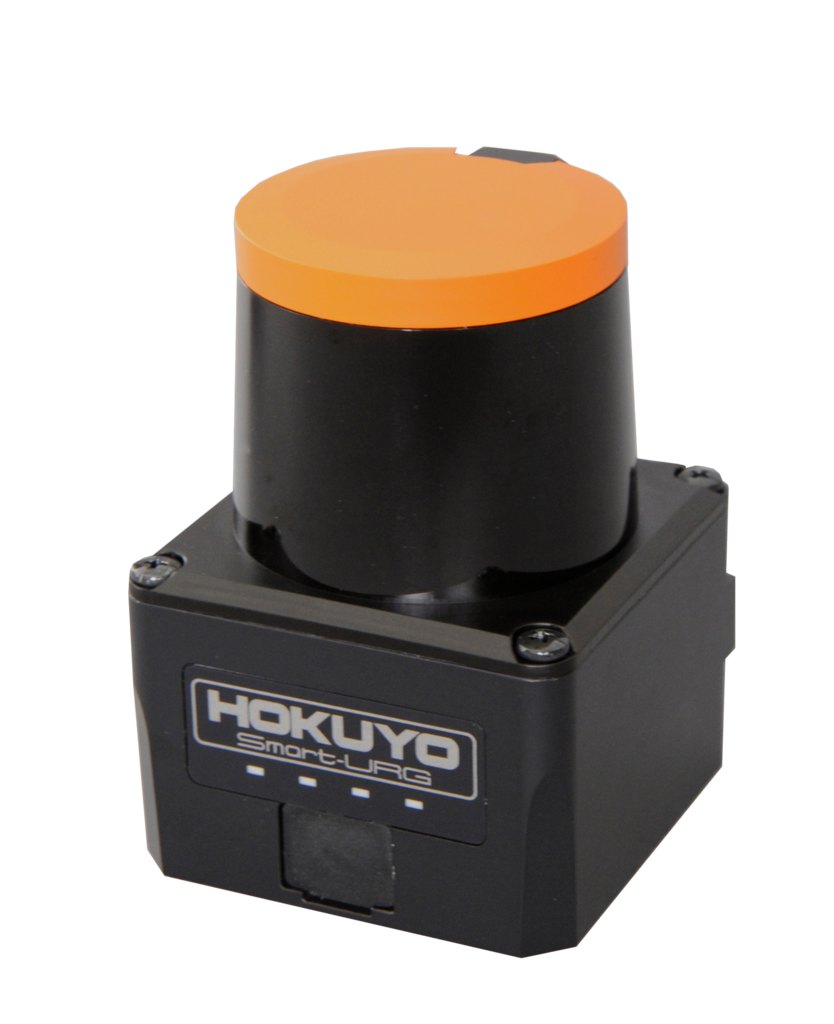
\includegraphics[width=\textwidth]{hokuyo_pic}
    \end{subfigure}
    \caption{The Hokuyo UST-10LX LIDAR}\label{fig:ur10}
\end{figure*}
This sensor uses a laser source to scan 270$^\circ$ field of view. Positions of objects in the range are calculated with step angle and distance. Sensor outputs these data through communication channel.

\section{FT300}
\begin{figure*}[h!]
    \centering
        \begin{subfigure}[h!,t]{0.34\textwidth}
        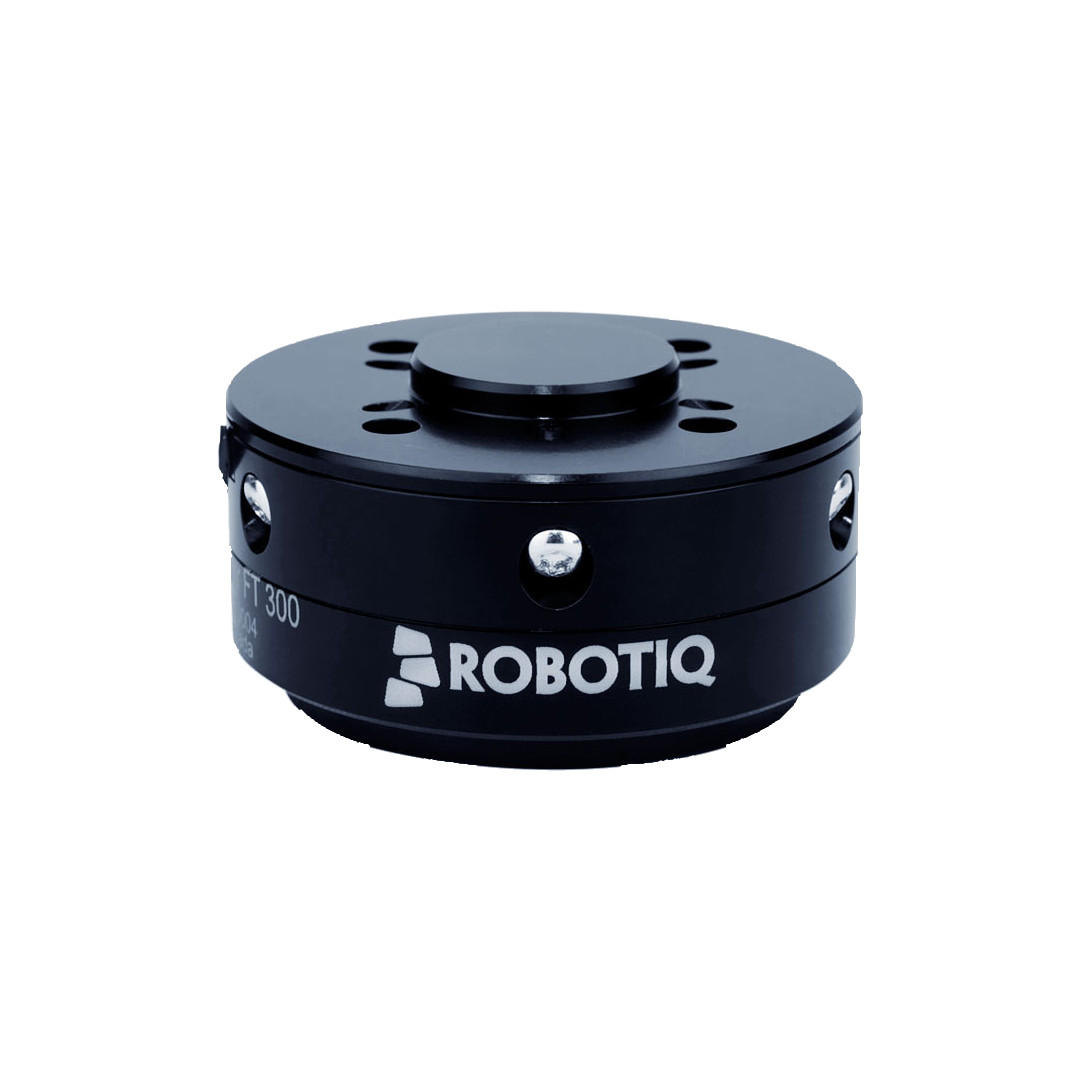
\includegraphics[clip, trim=0cm 5cm 0cm 5cm, width=\textwidth]{FT300_pic}
        \caption{Front}
        %\label{fig:gull}
    \end{subfigure}
    ~
    \begin{subfigure}[h!,t]{0.34\textwidth}
        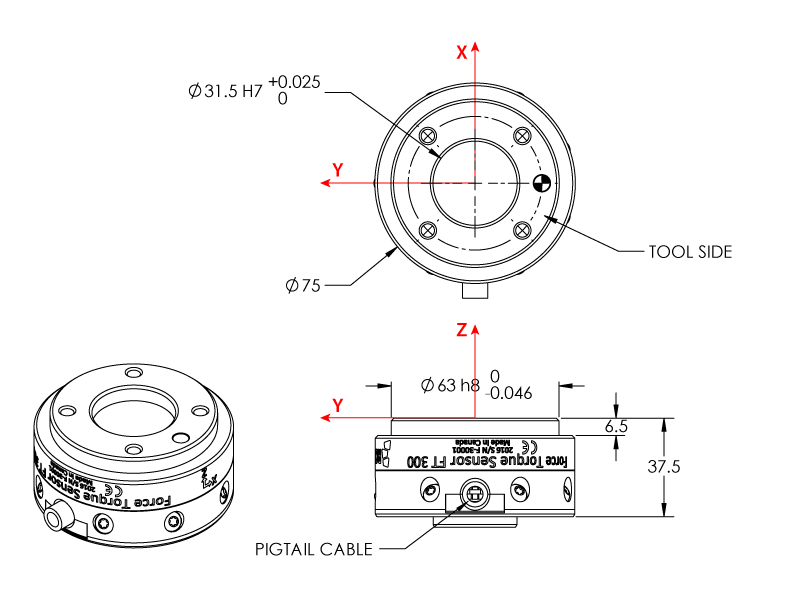
\includegraphics[width=\textwidth]{FT300}
        \caption{Side}
        %\label{fig:gull}
    \end{subfigure}
    \caption{The FT300 force-torque sensor}\label{fig:FT300}
\end{figure*}
The UR10 on the Thing mobile manipulator has a variety of sensors built-in for use in various tasks.
One such sensor is the FT300 force-torque sensor by Robotiq.
In terms of mechanical fit, the Sensor has an embedded coupling to fit directly on the UR wrist. The tool side of the Sensor matches the UR bolt pattern. 
It's application range from impedance control to perception and contact calibration of the manipulator.


\section{Robotiq Gripper}
\begin{figure}[h]
\centering
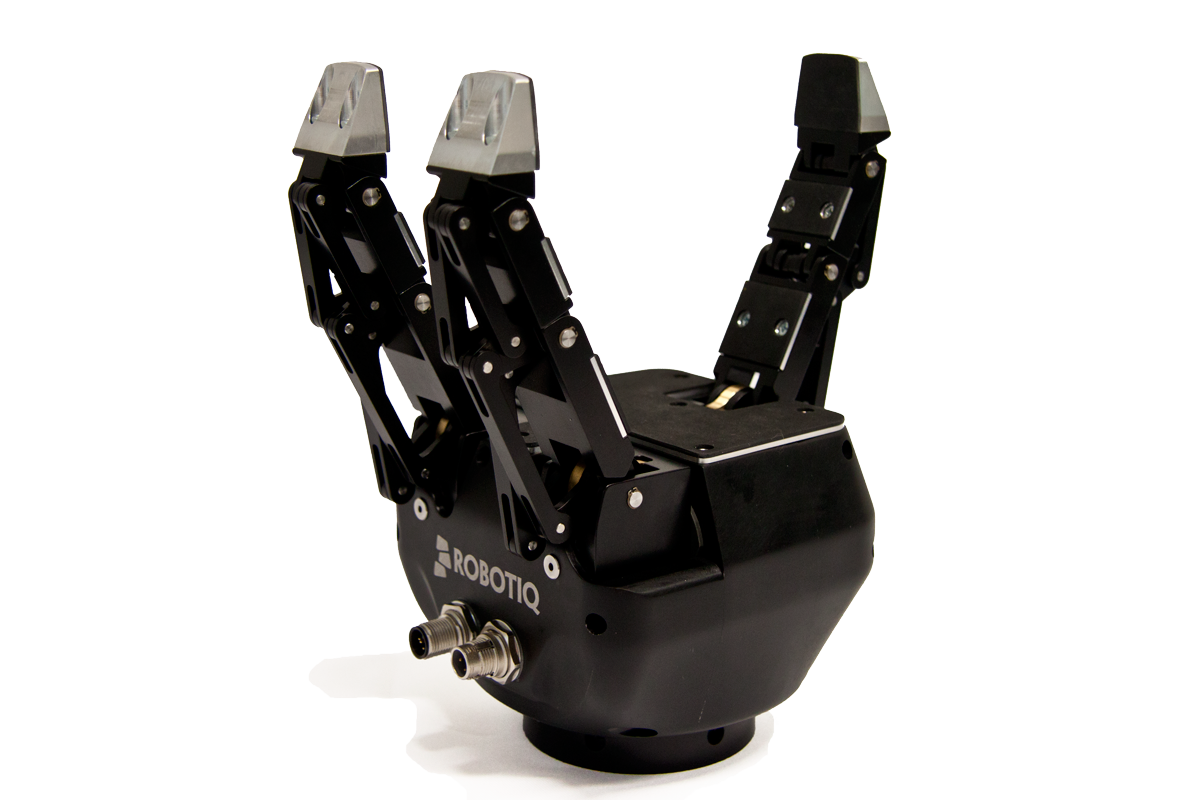
\includegraphics[width=0.3\textwidth]{robotiq}
\caption{The Robotiq gripper}
\end{figure}
The Robotiq gripper is a three-fingered adaptive gripper used as the end effector on the UR10 manipulator.
It is created for applications in advanced manufacturing and robotics research. 
All the fingers can be independently position,velocity and force controlled and can exert forces from 50 to 60 $N$ at the finger tips.

\chapter{Robot operating system}\label{sec:def_ROS}
ROS is an open source software development tool for implementing robotics software. It provides the opportunity of hardware abstraction, low level device control, implementation of commonly used functionalities, messages between different processes and package management. It provide tools and libraries which utilize the the opportunity of communicating between disturbed computers, obtaining, writing and running code.


ROS has three different levels of concepts

\begin{itemize}
\item \textbf{The file system level}

Handles the main unit for a ROS system which is packages. A package may include data sets, ROS dependent libraries, configure files etc. to define a ROS process. In ROS a process is denoted as a node. 
\item \textbf{The computation graph level}

Handles the communication of the peer to peer network of the system in which data is processed. Through the computation graph level, the different nodes can communicate with each other by messages. When a node is sending data it is said to be publishing a topic. The different nodes can then subscribe to this topic to get the information that is published.
\item \textbf{The Community level}

ROS has a huge community which contain distribution of software installations, repositories and documentation of ROS. It also has a question and answer section with ROS related topics.\\
This community makes the process of learning the system considerably easier.
\end{itemize}
\begin{abstract}
Abstract.

\keywords{Keywords.}
\end{abstract}

% TODO: Navedite naslov na hrvatskom jeziku.
\hrtitle{Naslov}
\begin{sazetak}
Sažetak na hrvatskom jeziku.

\kljucnerijeci{Ključne riječi, odvojene zarezima.}
\end{sazetak}

\end{document}
